%-----------------------------------------
% Note: Use pdflatex to process this file.
%
% IMPORTANT: This file uses .aux files from the Bmad manual so pdflatex the Bmad manual beforehand.
%            Note: It is assumed that the bmad and tao directories have the same parent directory.
%-----------------------------------------

\documentclass{book}
\usepackage{xr}       % Defines \externaldocument
\usepackage{graphicx}
\usepackage{moreverb}
\usepackage{amsmath}
\usepackage{alltt}
\usepackage{rotating}
\usepackage{subcaption}
\usepackage{xspace}
\usepackage{makeidx}
\usepackage{multirow}
\usepackage{booktabs}   % For table layouts
\usepackage{longtable}
\usepackage{enumitem} % enumeration lists

\usepackage[T1]{fontenc}   % so _, <, and > print correctly in text.
\usepackage[strings]{underscore}    % to use "_" in text
\usepackage{textcomp}
\usepackage[pdftex,colorlinks=true,bookmarksnumbered=true]{hyperref}  % This must be the last package

\newcommand{\hlabel}{\phantomsection\label}  % Used so hyper links will point to the spot where \hlabel is used.
\newcommand{\extref}[1]{$\S$\ref*{#1}}       % No hyperlink. For external refs. \extref
\newcommand{\pref}[1]{[\pageref{#1}]}

\newcommand{\comma}{\> ,}
\newcommand{\period}{\> .}
\newcommand{\wt}{\widetilde}
\newcommand{\grv}{\textasciigrave}
\newcommand{\hyperbf}[1]{\textbf{\hyperpage{#1}}}
\newcommand{\Ss}{\(^*\)}
\newcommand{\Dd}{\(^\dagger\)}

\newcommand{\fig}[1]{Fig.~\ref{#1}}
\newcommand{\figs}[1]{Figs.~\ref{#1}}

\newcommand{\AND}{&& \hskip -17pt\relax}
\newcommand{\CR}{\\}
\newcommand{\CRNO}{\nonumber \\}
\newcommand{\dstyle}{\displaystyle}
\newcommand{\NoPrint}[1]{}

\newcommand{\pow}[1]{\cdot 10^{#1}}
\newcommand{\Bf}[1]{{\bf #1}}
\newcommand{\bfr}{\Bf r}
\newcommand{\bfl}{\Bf l}
\newcommand{\bfm}{\Bf m}
\newcommand{\bfn}{\Bf n}
\newcommand{\bfq}{\Bf q}
\newcommand{\bfG}{\Bf G}
\newcommand{\bfD}{\Bf D}
\newcommand{\bfM}{\Bf M}
\newcommand{\bfsig}{{\boldsymbol{\sigma}}}
\newcommand{\arrowbfq}{\overrightarrow{\Bf q}}

\newcommand{\bmad}{{\sl Bmad}\xspace}
\newcommand{\tao}{{\sl Tao}\xspace}
\newcommand{\mad}{{\sl MAD}\xspace}
\newcommand{\cesr}{{\sl CESR}\xspace}

\newcommand{\sref}[1]{\S\ref{#1}}
\newcommand{\Sref}[1]{Sec.~\sref{#1}}
\newcommand{\cref}[1]{Chapter~\ref{#1}}

\newcommand{\Newline}{\hfil \\ \relax}

\newcommand{\eq}[1]{{(\protect\ref{#1})}}
\newcommand{\Eq}[1]{{Eq.~(\protect\ref{#1})}}
\newcommand{\Eqs}[1]{{Eqs.~(\protect\ref{#1})}}

\newcommand{\vn}{\ttcmd}           % For variable names
\newcommand{\vni}{\ttcmdindx}
\newcommand{\cs}{\ttcmd}           % For code source
\newcommand{\cmd}{\ttcmd}          % For Unix commands
\newcommand{\rn}{\ttcmd}           % For Routine names
\newcommand{\tn}{\ttcmd}           % For Type (structure) names
\newcommand{\bn}[1]{{\bf #1}}       
\newcommand{\toffset}{\vskip 0.01in}
\newcommand{\rot}[1]{\begin{rotate}{-45}#1\end{rotate}}
\newcommand{\tv}[1]{\text{\vn{#1}}}

\newcommand\ttcmd{\begingroup\catcode`\_=11 \catcode`\%=11 \dottcmd}
\newcommand\dottcmd[1]{\texttt{#1}\endgroup}

\newcommand\ttcmdindx{\begingroup\catcode`\_=11 \catcode`\%=11 \dottcmdindx}
\newcommand\dottcmdindx[1]{\texttt{#1}\endgroup\index{#1}}

\newcommand{\St}{$^{st}$\xspace}
\newcommand{\Nd}{$^{nd}$\xspace}
\newcommand{\Th}{$^{th}$\xspace}
\newcommand{\B}{$\backslash$}
\newcommand{\W}{$^\wedge$}

\newcommand{\cbar}[1]{\overline C_{#1}}

\newlength{\dPar}
\setlength{\dPar}{1.5ex}

\newenvironment{example}
  {\vspace{-3.0ex} \begin{alltt}}
  {\end{alltt} \vspace{-2.5ex}}

\newcommand\Strut{\rule[-2ex]{0mm}{6ex}}

\newenvironment{Itemize}
  {\begin{list}{$\bullet$}
    {\addtolength{\topsep}{-1.5ex}
     \addtolength{\itemsep}{-1ex}
     \addtolength{\partopsep}{-1ex}
    }
  }
  {\end{list} \vspace*{1ex}}

\newcommand{\Section}[1]{\section{#1}\indent\vspace{-3ex}}

\newcommand{\SECTION}[1]{\section*{#1}\indent\vspace{-3ex}}

% From pg 64 of The LaTex Companion.

\newenvironment{ventry}[1]
  {\begin{list}{}
    {\renewcommand{\makelabel}[1]{\textsf{##1}\hfil}
     \settowidth{\labelwidth}{\textsf{#1}}
     \addtolength{\itemsep}{-1.5ex}
     \addtolength{\topsep}{-1.0ex} 
     \setlength{\leftmargin}{5em}
    }
  }
  {\end{list}}


\externaldocument[B-]{../../bmad/doc/lattice-file}

\setlength{\textwidth}{6.25in}
\setlength{\oddsidemargin}{0.0in}
\setlength{\evensidemargin}{0.0in}
\setlength{\textheight}{8.5in}
\setlength{\topmargin}{0in}
\setlength{\skip\footins}{6pt}
\setlength{\footnotesep}{3ex}

\setlist[description]{itemsep = 0pt}

\renewcommand{\textfraction}{0.1}
\renewcommand{\topfraction}{1.0}
\renewcommand{\bottomfraction}{1.0}

%%% Table of Contents spacing.
\makeatletter
\renewcommand{\l@section}{\@dottedtocline{1}{1.5em}{3.3em}}
\renewcommand{\l@subsection}{\@dottedtocline{2}{3.8em}{4.2em}}
\renewcommand{\l@figure}{\@dottedtocline{1}{1.5em}{3.3em}}
\renewcommand{\l@table}{\@dottedtocline{1}{1.5em}{3.3em}}
\makeatother

%----------------------------------------------------------------
\makeindex

\begin{document}

\index{lattice!model|see{model lattice}}
\index{lattice!design|see{design lattice}}
\index{lattice!base|see{base lattice}}

\thispagestyle{empty}

\begin{flushright}
\large
Revision: September 15, 2025 \\
\end{flushright}

\vfill

{
\begin{center}
\resizebox{1.8cm}{!}{\Huge \sf\bf The} \\
\vskip 0.2in

\includegraphics[width=10cm]{tao-logo.pdf} \\
\vskip 0.3in
\resizebox{4.4cm}{!}{\Huge \sf\bf Manual} \\
\vskip 0.4in
{\huge \sf\bf David Sagan} \\
\end{center}
}

\vfill
\break


%----------------------------------------------------------------
{
\setlength{\parskip}{\dPar}
\setlength{\parindent}{0ex}
}

%----------------------------------------------------------------

\cleardoublepage
\phantomsection 
\pdfbookmark[0]{Contents}{Contents}
\pdfbookmark[1]{Table of Contents}{toc} 
\tableofcontents


\cleardoublepage
\phantomsection 
\pdfbookmark[1]{List of Figures}{LoF} 
\listoffigures


\cleardoublepage
\phantomsection 
\pdfbookmark[1]{List of Tables}{LoT} 
\listoftables

%----------------------------------------------------------------
\setlength{\parskip}{\dPar}
\setlength{\parindent}{0ex}

%----------------------------------------------------------------
\part{Reference Guide}
\label{ref-guide}

\chapter{Overview}
\label{c:overview}

%------------------------------------------------------------------------
\section{In the beginning...}
\label{s:overview}


\tao stands for ``Tool for Accelerator Optics''. \tao is a general purpose program for simulating
high energy particle beams in accelerators and storage rings. This manual assumes you are already
familiar with the basics of particle beam dynamics and its formalism. There are several books that
introduce the topics very well. A good place to start is, for example, \textit{The Physics of
Particle Accelerators} by Klaus Wille\cite{b:wille}.

\index{bmad}
The simulation engine that \tao uses for doing such things as particle tracking is the \bmad
software library\cite{b:bmad}. \bmad was developed as an object-oriented library so that common
tasks, such as reading in a lattice file and particle tracking, did not have to be coded from
scratch every time someone wanted to develop a program to calculate this, that or whatever.  An
understanding of the nitty-gritty details of the routines that comprise \bmad is not necessary,
however, one should be familiar with the conventions that \bmad uses and this is covered in the
\bmad manual.

\bmad was developed before \tao. As \bmad was being developed, it became apparent that many
simulation programs had common needs: For example, plotting data, viewing machine parameters,
etc. Because of this commonality, the \tao program was developed to reduce the time needed to
develop a working programs without sacrificing flexibility. That is, while the ``vanilla'' version
of the \tao program is quite a powerful simulation tool, \tao has been designed to be easily
customizable so that extending \tao to solve new and different problems is relatively straight
forward.

So, what is \tao good for? A large variety of applications: Single and multiparticle tracking,
lattice simulation and analysis, lattice design, machine commissioning and correction,
etc. Furthermore, it is designed to be extensible using interface ``hooks'' built into the program.
This versatility has been used, for example, to enable \tao to directly read in measurement data
from Cornell's Cesr storage ring and Jefferson Lab's FEL. Think of \tao as an accelerator design and
analysis environment. But even without any customizations, \tao will do much analysis.

More information, including the most up--to--date version of this manual, can be found at the \bmad
web site at:
\begin{example}
  classe.cornell.edu/bmad
\end{example}

Errors and omissions are a fact of life for any reference work and comments from you, dear reader,
are therefore most welcome. Please send any missives (or chocolates, or any other kind of
sustenance) to:
\begin{example}
  David Sagan <dcs16@cornell.edu>
\end{example}

It is my pleasure to express appreciation to people who have contributed to this effort. To Scott
Berg, Michael Ehrlichman, Chris Mayes, and Jeff Smith for bug reports, suggestions, code
improvements, Etc. To John Mastroberti and Kevin Kowalski for their work on a graphics user
interface and associated plotting, And last but not least thanks also must go to Dave Rubin and
Georg Hoffstaetter for their help, support, and patience.

%------------------------------------------------------------------------
\section{Bmad and Tao Tutorial}
\label{s:tutorial}

\vspace{0.1in} The \tao manual is organized as reference guide and so does not do a good job of
instructing the beginner as to how to use \tao. For this there is an introduction and tutorial on
\bmad and \tao concepts that can be downloaded from the \bmad web page. Go to either the \bmad
manual or the \tao manual page and there will be a link for the tutorial.

%------------------------------------------------------------------------
\section{Tao Examples}
\label{s:examples}

Example input files for running a number of different simulations can be found with the \bmad and \tao
Tutorial (\sref{s:tutorial}). Additionally, there are a number of examples in the directory
\begin{example}
  \$ACC_ROOT_DIR/bmad-doc/tao_examples/
\end{example}
where \vn{\$ACC_ROOT_DIR} is the base directory of your local \bmad Distribution or Release (a full
description of \bmad Distributions and Releases is given in the \bmad and \tao Tutorial).

%------------------------------------------------------------------------
\section{Manual Organization}

This manual is divided into two parts. Part I is the reference section which defines the terms used
by \tao, discusses \tao commands, etc. Part II is a programmer's guide which shows how to extend
\tao's capabilities including interfacing to Python and how to incorporate custom calculations into
\tao.

%------------------------------------------------------------------------
\section{Other Bmad based programs}
\label{s:other}

\tao is not the only program based upon \bmad. There are other programs which are specialized for
certain computations such as long-term tracking, beam break-up instability, multi-objective
optimization, etc. The discussion of these programs is beyond the scope of this manual. More
information along with instructions for obtaining the programs can be obtained from the \bmad web site (\sref{s:overview}).


\chapter{Introduction}
\label{c:introduction}

%----------------------------------------------------------------
\section{Obtaining Tao}
\index{tao!Obtaining}
\label{s:obtaining}

A \vn{Distribution} is a set of files, including \bmad and \tao source files, which are used to
build the \bmad, the \tao program, and various other simulation programs. A \vn{Release} is like a
\vn{Distribution} except that it is created on the Linux computer system at CLASSE (Cornell's
Laboratory for Accelerator-based Sciences and Education). More information can be obtained from the
\bmad web site. 

If there is no local \bmad Guru to guide you, download and setup instructions for downloading a
Distribution, environment variable setup, and building \tao is contained on the \bmad web
site and will not be covered here.

%----------------------------------------------------------------
\section{Starting and Initializing Tao}
\index{initializing!files}
\label{s:initializing}

The syntax for starting \tao is given in \Sref{s:command.line}.

Initialization occurs when \tao is started. Initialization information is stored in one or more
files as discussed in Chapter \sref{c:init}.

%%----------------------------------------------------------------
\section{Running Tao with OpenMP}
\index{openMP}
\label{s:openmp}

\vn{OpenMP} is a standard that enables programs to run calculations with multiple threads which will
reduce computation time. Certain calculations done by \tao, including beam tracking and dynamic
aperture calculations, can be run multithreaded via OpenMP if the \tao executable file has been
properly compiled.  Interested users should consult their local \bmad Guru for guidance. Note:
\vn{OpenMP} multithreading involves using multiple cores of a single machine (unlike \vn{Open MPI}
which involves multiple machines). Therefore, it is not necessary to have a cluster of machines to
use \vn{OpenMP}.

To set the number of threads when running a program compiled with \vn{OpenMP}, set the environment variable
\vn{OMP_NUM_THREADS}. Example:
\begin{example}
  export OMP_NUM_THREADS=8
\end{example}

This may also be set during Tao runtime as the global parameter \vn{n_threads}. For example:
\begin{example}
  set global n_threads = 1  ! Use only a single thread
  set global n_threads = 4  ! Use four threads
\end{example}

See \sref{s:set.global} for more information.

To the local \bmad Guru: Compiling and linking of \tao with \vn{OpenMP} is documented on the \bmad
web site. By default, \vn{OpenMP} is not enabled. Essentially, OpenMP is enabled by modifying
the \vn{dist_prefs} file before compiling and linking.

%----------------------------------------------------------------
\section{Command Line Mode and Single Mode}
\label{s:modes}

After \tao is initialized, \tao interacts with the user though the command line. \tao has two modes
for this. In \vn{command line} mode, which is the default mode, \tao waits until the the \vn{return}
key is depressed to execute a command. Command line mode is described in Chapter~\sref{c:command}. 

In \vn{single} mode, single keystrokes are interpreted as commands. \tao can be set up so that in
\vn{single mode} the pressing of certain keys increase or decrease variables. While the same effect
can be achieved in the standard \vn{line mode}, \vn{single mode} allows for quick adjustments of
variables. See Chapter~\sref{c:single} for more details.

%-----------------------------------------------------------------
\section{Lattice Calculations}
\index{lattice calculaitons}
\label{s:lat.calc.overview} 

By default \tao recalculates lattice parameters and does tracking of particles after each command.
The exception is for commands that do not change any parameter that would affect such calculations
such as the \vn{show} command. See \sref{s:lat.calc} for more details. If the recalculation takes a
significant amount of time, the recalculation may be suppressed using the \vn{set global
lattice_calc_on} command (\sref{s:set.global}) or the \vn{set universe} command
(\sref{s:set.universe}).

%-----------------------------------------------------------------
\section{Command Files and Aliases}
\index{command files}
\label{s:command.files} 

Typing repetitive commands in command line mode can become tedious. \tao has two constructs to
mitigate this: Aliases and Command Files. 

Aliases are just like aliases in Unix. See Section~\sref{s:alias} for more details.

Command files are like Unix shell scripts. A series of commands are
put in a file and then that file can be called using the \vn{call}
command (\sref{s:call}).

\tao will call a command file at startup. The default name of this startup file is \vn{tao.startup}
but this name can be changed (\sref{s:format}).

Do loops (\sref{s:do}) are allowed with the following syntax:
\begin{example}
  do <var> = <begin>, <end> \{, <step>\} 
    ...
    tao command [[<var>]]
    ...
  enddo
\end{example}
The \vn{<var>} can be used as a variable in the loop body but must be
bracketed ``[[<var>]]''.  The step size can be any integer positive or
negative but not zero.  Nested loops are allowed and command files can
be called within do loops.

\begin{example}
  do i = 1, 100
    call set_quad_misalignment [[i]] ! command file to misalign quadrupoles
    zero_quad 1e-5*2^([[i]]-1) ! Some user supplied command to zero quad number [[i]]
  enddo
\end{example}

To reduce unnecessary calculations, the logicals \vn{global%lattice_calc_on}
and \vn{global%plot_on} can be toggled from within the command file. Also 
setting \vn{global%quiet} can turn off verbose output to the terminal. 
Note: Setting \vn{global%lattice_calc_on} to False will also disable any plotting
calculations. 
Example
\begin{example}
  set global quiet = all          ! Turn off verbose output to the terminal.
  set global lattice_calc_on = F  ! Turn off lattice  and plotting calculations
  ... do some stuff ...
  set global lattice_calc_on = T  ! Turn back on
  set global quiet = off         
\end{example}
See \sref{s:globals} for more details.

A \vn{end_file} command (\sref{s:end.file}) can be used to signal the
end of the command file.

The \vn{pause} command (\sref{s:pause}) can be used to temporarily
pause the command file.


\chapter{Organization and Structure}
\label{c:organization}

This chapter discusses how \tao is organized. After you are familiar with the basics of \tao, you
might be interested to exploit its versatility by extending \tao to do custom calculations. For
this, see Chapter~\ref{c:custom.tao}.

%----------------------------------------------------------------
\section{The Organization of Tao: The Super\_Universe}
\label{s:organization}
\index{super_universe}

Many simulation problems fall into one of three categories: 
\begin{itemize}
\item 
Design a lattice subject to various constraints.
\item
Simulate errors and changes in machine parameters. For example, you want to simulate what happens to
the orbit, beta function, etc., when you change something in the machine.
\item 
Simulate machine commissioning including simulating data measurement and correction. For example,
you want to know what steering strength changes will make an orbit flat.
\end{itemize}
Programs that are written to solve these types of problems have common elements: You have variables
you want to vary in your model of your machine, you have "data" that you want to view, and, in the
first two categories above, you want to match the machine model to the data (in designing a lattice
the constraints correspond to the data).

With this in mind, \tao was structured to implement the essential ingredients needed to solve these
simulation problems.  The information that \tao knows about can be divided into five (overlapping)
categories:
\begin{description}
  \index{lattice}
  \item[Lattice] \Newline   
Machine layout and component strengths, and the beam orbit (\sref{s:lattice}).
  \index{data}
  \item[Data] \Newline
Anything that can be measured.
For example: The orbit of a particle or the lattice beta 
functions, etc. (\sref{c:data})
  \index{variable}
  \item[Variables] \Newline
Essentially, any lattice parameter or initial condition that can be varied. For example: quadrupole
strengths, etc. (\sref{c:var}).
  \index{plotting}
  \item[Plotting]  \Newline
Information used to draw graphs, display the lattice 
floor plan, etc. (\sref{c:plotting}).
  \index{global parameters}
  \item[Global Parameters] \Newline
 \tao has a set of parameters to control every aspect of how it behaves from
the random number seed \tao uses to what optimizer is used for fitting data.
\end{description}

%------------------------------------------------------------------------
\section{The Super\_universe}
\label{s:super.uni}
\index{super_universe|hyperbf}

\index{structure|hyperbf}
The information in \tao deals is organized in a hierarchy of \vn{``structures''}. At the top level,
everything known to \tao is placed in a single structure called the \vn{super_universe}.

\index{universe}
\index{variable}
Within the \vn{super_universe}, lies one or more \vn{universes} (\sref{s:universe}), each
\vn{universe} containing a particular machine lattice and its associated data. This allows for the
user to do analysis on multiple machines or multiple configurations of a single machine at the same
time. The \vn{super_universe} also contains the \vn{variable}, \vn{plotting}, and \vn{global
parameter} information.

%------------------------------------------------------------------------
\section{The Universe}
\label{s:universe}
\index{universe|hyperbf}

\index{lattice}\index{design lattice}\index{model lattice}
\index{base lattice}\index{data}\index{super_universe}
The \tao \vn{super_universe} (\sref{s:super.uni}) contains one or more \vn{universes}.  A
\vn{universe} contains a \vn{lattice} (\sref{s:lattice}) plus whatever data (\sref{c:data}) one
wishes to study within this lattice (i.e. twiss parameters, orbit, phase, etc.). Actually, there are
three lattices within each universe: the \textbf{design} lattice, \textbf{model} lattice and
\textbf{base} lattice. Initially, when \tao is started, all three lattices are identical and
correspond to the lattice read in from the lattice description file (\sref{s:init.lat}).

There are several situations in which multiple universes are useful. One case where multiple
universes are useful is where data has been taken under different machine conditions. For example,
suppose that a set of beam orbits have been measured in a storage ring with each orbit corresponding
to a different steering element being set to some non-zero value. To determine what quadrupole
settings will best reproduce the data, multiple universes can be setup, one universe for each of the
orbit measurements. Variables can be defined to simultaneously vary the corresponding quadrupoles in
each universe and \tao's built in optimizer can vary the variables until the data as determined from
the \vn{model} lattice (\sref{s:lattice}) matches the measured data. This \vn{orbit response matrix}
(ORM) analysis is, in fact, a widely used procedure at many laboratories.

If multiple universes are present, it is important to be able to specify, when issuing commands to
tao and when constructing \tao initialization files, what universe is being referred to when
referencing parameters such as data, lattice elements or other stuff that is universe
specific. [Note: \tao variables are {\em not} universe specific.] If no universe is specified with a
command, the \vn{default} universe will be used. This default universe is set set by the \vn{set
default universe} command (\sref{s:set}). When \tao starts up, the default universe is initially set
to universe 1. Use the \vn{show global} (\sref{s:show}) command to see the current default universe.

the syntax used to specify a particular universe or range of universes is attach a prefix of the
form:
\begin{example}
  [<universe_range>]@<parameter>
\end{example}
Commas and colons can be used in the syntax for \vn{<universe_range>}, similar to the \vn{element
list} format used to specify lattice elements (\sref{s:ele.list.format}).  When there is only a
single Universe specified, the brackets \vn{[...]} are optional. When the universe prefix is not
present, the current default universe is used. The current default universe can also be specified
using the number \vn{-1}. Additionally, a ``\vn{*}'' can be used as a wild card to denote all of the
universes. Examples:
\begin{example}
  [2:4,7]@orbit.x ! The \vn{orbit.x} data in universes 2, 3, 4 and 7.
  [2]@orbit.x     ! The \vn{orbit.x} data in universe 2. 
  2@orbit.x       ! Same as "2@orbit.x".
  orbit.x         ! The \vn{orbit.x} data in the current default universe.
  -1@orbit.x      ! Same as "orbit.x".
  *@orbit.x       ! orbit.x data in all the universes.
  *@*             ! All the data in all the universes. 
\end{example}

%------------------------------------------------------------------------
\section{Lattices}
\index{lattice|hyperbf}
\label{s:lattice}

\index{design lattice}\index{model lattice}
\index{base lattice}
A \vn{lattice} consists of a machine description (the strength and placement of elements such as
quadrupoles and bends, etc.), along with the beam orbit through them. There are actually three types
of lattices:
  \vspace*{-3ex}
  \begin{description}
  \index{design lattice|hyperbf}
  \item[Design Lattice] \Newline 
The \vn{design} lattice corresponds to the lattice read in from the lattice description file(s)
(\sref{s:init.lat}). In many instances, this is the particular lattice that one wants the actual
physical machine to conform to. The \vn{design} lattice is fixed. Nothing is allowed to vary in this
lattice.
  \index{model lattice|hyperbf}
  \item[Model Lattice] \Newline
Initially the \vn{model} lattice is the same as the \vn{design} lattice. Except for some commands
that explicitly set the \vn{base} lattice, all \tao commands to vary lattice variables vary
quantities in the \vn{model} lattice. In particular, things like orbit correction involve varying
\vn{model} lattice variables until the \vn{data}, as calculated from the \vn{model}, matches the
\vn{data} as actually measured.
  \index{base lattice|hyperbf}
  \index{base lattice!using set command}
  \item[Base Lattice] \Newline
It is sometimes convenient to designate a reference lattice so that changes in the \vn{model} from
the reference point can be examined.  This reference lattice is called the \vn{base} lattice. The
\vn{set} command (\sref{s:set}) is used to transfer information from the \vn{design} or \vn{model}
lattices to the base lattice. Initially, the \vn{base} lattice is set equal to the \vn{design}
lattice by \tao.
  \end{description}

Lattices can have multiple \vn{branches}. For example, two intersecting rings can be represented as
a lattice with two branches, one for each ring. See the \bmad manual for more details. Many \tao
commands operate on a particular lattice branch. For example, the \vn{show lat} command prints the
lattice elements of a particular branch. If no branch is specified with a command, the default
branch is used. The default branch is set with the \vn{set default branch} command
(\sref{s:set}). Initially, when \tao is started, the default branch is set to branch 0. Use the
\vn{show global} (\sref{s:show}) command to see the current default branch.

%------------------------------------------------------------------------
\section{Tracking Types}
\index{tracking!types}

\index{track_type}
\index{tao_global_struct}
\index{global%track_type}
The are two types of tracking implemented in \tao: single particle tracking and many particle
multi-bunch tracking.  Single particle tracking is just that, the tracking of a single particle
through the lattice. Many particle multi-bunch tracking creates a Gaussian distribution of particles
at the beginning of the lattice and tracks each particle through the lattice, including any
wakefields.  Single particle tracking is used by default. The \vn{global%track_type} parameter
(\sref{s:globals}), which is set in the initialization file, is used to set the tracking.

Particle spin tracking has also been set up for single particle and many particle tracking. See
Sections~\sref{s:globals} and \sref{s:beam.init} for details on setting up spin tracking.

%------------------------------------------------------------------------
\section{Lattice Calculation}\index{lattice!calculation of}
\label{s:lat.calc}

After each \tao command is processed, the lattice and ``merit'' function are recalculated and the
plot window is regenerated. The merit function determines how well the \vn{model} fits the measured
data. See Chapter~\ref{c:opti} for more information on the merit function and its use by the
optimizer.

Below are the steps taken after each \tao command execution:
\begin{enumerate}
  \item 
The data and variables used by the optimizer are re-determined. This is affected by commands such as
\vn{use, veto,} and \vn{restore} and any changes in the status of elements in the ring (e.g. if any
elements have been turned off).
  \item 
If changes have been made to the lattice (e.g. variables changed) then the model lattice for all
universes will be recalculated. The \vn{model} orbit, linear transfer matrices and Twiss parameters
are recalculated for every element. All data types will also be calculated at each element specified
in the initialization file.  For single particle tracking the linear transfer matrices and Twiss
parameters are found about the tracked orbit. Tracking is performed using the tracking method
defined for each element (i.e. Bmad Standard, Symplectic Lie, etc...). See the \bmad Reference
manual for details on tracking and finding the linear transfer matrices and Twiss parameters.
  \item 
The \vn{model} data is recalculated from the \vn{model} orbit, linear transfer matrices, Twiss
parameters, particle beam information and global lattice parameters.  Any custom data type
calculations are performed \textit{before} the standard \tao data types are calculated.
  \item 
Any user specified data post-processing is performed in
\vn{tao_hook_post_process_data}.
  \item 
The contributions to the merit function from the variables and data are computed.
  \item 
Data and variable values are transferred to the plotting structures.
  \item 
The plotting window is regenerated.
\end{enumerate}

If a closed orbit is to be calculated, \tao uses an iterative method to converge on a solution where
\tao starts with some initial orbit at the beginning of the lattice, tracks from this initial orbit
through to the end of the lattice, and then adjusts the beginning orbit until the end orbit matches
the beginning orbit. A problem arises if the tracked particle is lost before it reaches the end of
the lattice since \tao has no good way to calculate how to adjust the beginning orbit to prevent the
particle from getting lost. In this case, \tao, in desperation, will try the orbit specified by
\vn{particle_start} in the \bmad lattice file (see the \bmad manual for more details on setting
\vn{particle_start}). Note: \vn{particle_start} can be varied while running \tao using the \vn{set
particle_start} (\sref{s:set}) or \vn{change particle_start} (\sref{s:change}) commands.

If the recalculation takes a significant amount of time, the recalculation may be suppressed using
the \vn{set global lattice_calc_on} command (\sref{s:set.global}) or the \vn{set universe} command
(\sref{s:set.universe}).

\chapter{Syntax}
\label{c:syntax}

%------------------------------------------------------------------------
\section{Command Line Syntax}
\label{s:com.syntax}

In ``\vn{line mode}'' (\sref{c:command}), commands are case sensitive. Multiple commands may be
entered on one line using the semicolon ``;'' character as a separator.  [However, a semicolon used
as as part of an \vn{alias} (\sref{s:alias}) definition is part of that definition.]  An exclamation
mark ``\vn{!}''  denotes the beginning of a comment and the exclamation mark and everything after it
to the end of the line is ignored.  Example:
\begin{example}
  set default uni = 2; show global  ! Two commands and a comment
\end{example}

The length of a command on a single line is currently limited to 1000 characters. Multiple lines may
be used for a single command by putting a ``\&'' character at the end of a line to be
continued. Example:
\begin{example}
  set default &    ! Continue command to next line
  uni = 2
\end{example}

Note that, for historical reasons, Bmad itself is case insensitive. Thus things like lattice element 
names within \tao commands will similarly be case insensitive.

%------------------------------------------------------------------------
\section{Specifying a Single Lattice Element}
\label{s:ele.name}

A full description of how to specify a lattice element is given in section \extref{B-s:ele.match}
``\vn{Matching to Lattice Element Names}'' in the \bmad manual. Generally, elements are specified
using either their names or by their index number. Additionally, in \tao, the universe in which
the element exists may be specified by prepending the element name by the universe number followed by
the ``\vn{@}'' sign.
Examples:
\begin{example}
  Q3##2      ! 2nd instance of element named Q3 in branch 0 of the default universe.
  134        ! Element with index 134 in branch 0 of the default universe.
  1>>13      ! Element with index 13 in branch 1 of the default universe.
  2@1>>TZ    ! Element named TZ in branch 1 of universe 2.
  B37        ! Element named B37 of the default universe.
  0@B37      ! Same as the previous example.
\end{example}
Note: element names are {\em not} case sensitive.

%------------------------------------------------------------------------
\section{Lattice Element List Format}
\label{s:ele.list.format}

The syntax for specifying a set of lattice elements is called \vn{element list} format. 
A element list is a list of items separated by a comma.\footnote
  {
 A blank space may be acceptable in some circumstances but a comma is always safe.
  }
Each item of the list is one of:
\begin{center}
\begin{tabular}{ll}
  {\it Item Type} & {\it Example} \\ \hline     
  A single element (\sref{s:ele.name})                & "1>>Q10W"            \\
  A name with wild card characters                    & "5@q*"               \\
  A range of elements in the form <ele1>:<ele2>       & "b23w:67"            \\
  A class::name specification                         & "sbend::b*"          \\
\end{tabular}
\break
\end{center}

Example element list:
\begin{example}
  23, 45:74, quad::q*
\end{example}

The wild card characters ``*'' and/or ``\%'' can be used. The ``*'' wildcard matches any number of
characters, The ``\%'' wildcard matches a single character. For example, ``q\%1*'' matches any
element whose name begins with ``q'' and whose third character is ``1''.  If there are multiple
elements in the lattice that match a given name, all such elements are included. Thus ``d12'' will
match to all elements of that name. Examples
\begin{example}
  "134"        ! Element with index 134 in branch 0 of the default universe.
  "1>>13"      ! Element with index 13 in branch 1 of the default universe.
  "5@q*"       ! All elements whose name begins with "q" of universe 5.
  "2@3>>q1##4" ! The fourth element named "q1" in branch 3 of universe 2.
  "*@sex10w"   ! Element "sex10w" of all universes.
  "b37"        ! Element "b37" of the default universe.
  "0@b37"      ! Same as the previous example.
\end{example}
Note: element names are {\em not} case sensitive.

An element index item is simply the index of the number in the lattice list of elements. A prefix
followed by the string ">>" can be used to specify a branch. As with element names, a universe
prefix can be given. Example
\begin{example}
  2@3>>183   ! Element number 183 of branch \# 3 of universe 2.
\end{example}

A range of elements is specified using the format:
\begin{example}
  \{<class>::\}<ele1>:<ele2>
\end{example}
\vn{<ele1>} is the element at the beginning of the range and \vn{<ele2>} is the element at the end
of the range. Either an element name or index can be used to specify \vn{<ele1>} and
\vn{<ele2>}. Both \vn{<ele1>} and \vn{<ele2>} are part of the range. The optional \vn{<class>}
prefix can be used to select only those elements in the range that match the class.  Example:
\begin{example}
  quad::sex10w:sex20w
\end{example}
This will select all quadrupoles between elements \vn{sex10w} and \vn{sex20w}.

\index{class::name}
A \vn{class::name} item
selects elements based upon their class (Eg: \vn{quadrupole},
\vn{marker}, etc.), and their name. The syntax is:
\begin{example}
  <element class>::<element name>
\end{example}
where \vn{<element class>} is an element class and \vn{<element name>} is the element name that can
(and generally does) contain the wild card characters ``\%'' and ``*''. Essentially this is an
extension of the \vn{element name} format. As with element names, a universe prefix can be
given. Example:
\begin{example}
  "4@quad::q*"   ! All quadrupole whose name starts with "q" of universe 4.
\end{example}

%------------------------------------------------------------------------
\section{Arithmetic Expressions}
\index{arithmetic Expressions}
\label{s:arithmetic.exp}

\tao is able to handle arithmetic expressions within commands (\sref{c:command}) and in strings in a
\tao initialization file.  Arithmetic expressions can be used in a place where a real value or an
array of real values are required.  The standard binary operators are defined: \hfil\break \hspace*{0.15in}
\begin{tabular}{ll}
  $a + b$           & Addition        \\
  $a - b$           & Subtraction     \\
  $a \, \ast \, b$  & Multiplication  \\
  $a \; / \; b$     & Division        \\
  $a \, \land \, b$ & Exponentiation  \\
\end{tabular} \newline
The following intrinsic functions are also recognized (this is the same list as the \bmad parser):
\hfil\break
\index{intrinsic functions}
\hspace*{0.15in}
\begin{tabular}{ll}
  \vn{sqrt}(x)                & Square Root                      \\
  \vn{log}(x)                 & Logarithm                        \\
  \vn{exp}(x)                 & Exponential                      \\
  \vn{sin}(x), \vn{cos}(x)    & Sine and Cosine                  \\
  \vn{tan}(x), \vn{cot}(x)    & Tangent and Cotangent            \\
  \vn{asin}(x), \vn{acos}(x)  & Arc sine and Arc Cosine          \\
  \vn{atan}(y)                & Arc Tangent                      \\
  \vn{atan2}(y, x)            & Arc Tangent                      \\
  \vn{abs}(x)                 & Absolute Value                   \\
  \vn{factorial(x)}           & Factorial                        \\
  \vn{ran}()                  & Random number between 0 and 1    \\
  \vn{ran_gauss}()            & Gaussian distributed random number with unit RMS \\
  \vn{ran_gauss}(sig_cut)     & Gaussian distributed random number truncated at sig_cut. \\
  \vn{int(x)}                 & Nearest integer with magnitude less then x \\
  \vn{nint(x)}                & Nearest integer to x             \\
  \vn{floor(x)}               & Nearest integer less than x      \\
  \vn{ceiling(x)}             & Nearest integer greater than x   \\
  \vn{modulo(a, p)}           & a - floor(a/p) * p. Will be in range [0, p]. \\
  \vn{average(arr)}           & Average value of an array        \\
  \vn{rms(arr)}               & RMS value of an array            \\
  \vn{sum(arr)}               & Sum of array values.             \\
  \vn{min(arr)}               & Minimum of array values.         \\
  \vn{max(arr)}               & Maximum of array values.         \\
  \vn{mass_of}(A)               & Mass of particle A             \\
  \vn{charge_of}(A)             & Charge, in units of the elementary charge, of particle A \\
  \vn{anomalous_moment_of}(A)   & Anomalous magnetic moment of particle A        \\
  \vn{species}(A)               & Integer ID associated with species A
\end{tabular} \newline
Both \vn{ran} and \vn{ran_gauss} use a seeded random number generator.  Setting the seed is
described in Section~\sref{s:globals}.

Expressions may involve arrays of values. For example:
\begin{example}
  lat::orbit.x[5:8]     ! X-orbit at lattice elements 5 through 8.
  [1, 2, 3]             ! A vector of size three.
\end{example}
When using vectors with binary operators or intrinsic functions, the standard rules apply. For example:
\begin{example}
  s * [a, b, c]         = [s*a, s*b, s*c]
  [a, b, c] - [x, y, z] = [a-x, b-y, c-z]
  tan([a, b, c])        = [tan(a), tan(b), tan(c)]
  sum([a, b, c])        = a+b+c
  min(a, b, c)          ! Error: Correct is min([a, b, c])
\end{example}
Note that \tao does not make a distinction between a scalar and a vector of length one.

See the following sections for the syntax for using data, variable, and lattice parameters in an
expression. Use the \vn{show value} command (\sref{s:show.value}) to show the results of expressions.

%------------------------------------------------------------------------
\section{Specifying Data Parameters in Expressions}
\label{s:data.token}

A data (\sref{s:data.org}) parameter ``\vn{token}'' is a string that specifies a scalar or an array
of data parameters.  The general form for data tokens in expressions (\sref{s:arithmetic.exp}) is:
\begin{example}
  \{[<universe(s)>]@\}data::<d2.d1_name>[<index_list>]|<component>
\end{example}
where:
\begin{example}
  <universe(s)>       Optional universe specification (\sref{s:universe})
  <d2.d1_name>        D2.D1 data name
  <index_list>        List of indexes.
  <component>         Component. 
\end{example}
examples:
\begin{example}
  [2:4,7]@data::orbit.x      ! The \vn{orbit.x} data in universes 2, 3, 4 and 7.
  [2]@data::orbit.x          ! The \vn{orbit.x} data in universe 2. 
  2@data::orbit.x[4]         ! Fourth \vn{orbit.x} datum in universe 2.
  data::orbit.x[4,7:9]|meas  ! Default uni measured values of datums 4, 7, 8, and 9.
  *@data::orbit.x            ! orbit.x data in all the universes.
  *@data::*                  ! All the data in all the universes.
\end{example}

It is important to keep in mind that data must be defined at startup in the appropriate
initialization file as discussed in \Sref{s:init.data} before reference is made to data in an
expression. The \vn{<d2.d1_name>} data names that have been defined at initialization time may be
viewed using the \vn{show data} command. Note that these names are user defined and do not have to
correspond to the data types given in \Sref{s:data.types}. See \Sref{s:lat.token} for how to use
``lattice parameters'' that correspond to the data types given in \Sref{s:data.types} and that do
not need to be defined at initialization.

See \Sref{s:data.anatomy} for a list of datum \vn{<component>}s (when running \tao, view a
particular datum with the \vn{show data} command to see the list).

\vn{<index_list>} is a list of indexes. \vn{<index_list>} will determine how many elements are in
the array. For example, \vn{orbit.x[10:21,44]} represents an array of 13 elements.

Depending upon the context, some parts of a token may be omitted. For example, with the \vn{set
data} command the ``\vn{data::}'' part of the token may be omitted.  Example:
\begin{example}
  set data 2@orbit.x|meas = var::quad_k1[5]|model - orbit.y[3]|ref
\end{example}
Here \tao will default to evaluating a token as data. In general, what may be omitted
should be clear in context.

Data components that are computed by \tao may be used on the right hand side of an equal sign but
may not be set. For example, the \vn{model} value of a datum is computed by \tao but the \vn{ref}
value is not.

If multiple tokens are used in an expression, all tokens must evaluate to arrays of the same size.

%------------------------------------------------------------------------
\section{Specifying Variable Parameters in Expressions}
\label{s:var.token}

A variable (\sref{c:var}) parameter ``\vn{token}'' is a string that specifies a scalar or an array
of variable parameters. The general form for variable tokens in expressions
(\sref{s:arithmetic.exp}) is:
\begin{example}
  var::<v1_name>[<index_list>]<component>
\end{example}
where:
\begin{example}
  <universe(s)>       Optional universe specification (\sref{s:universe})
  <v1_name>           V1 variable name.
  <index_list>        List of indexes.
  <component>         component. 
\end{example}
Examples:
\begin{example}
  var::*                     ! All the variables
  var::quad_k1[*]|design     ! All design values of quad_k1.
  var::quad_k1[]|model       ! No values. That is, the empty set.
  var::quad_k1|model         ! Same as quad_k1[*]|model
\end{example}

It is important to keep in mind that variables must be defined at startup in the appropriate
initialization file as discussed in \Sref{s:init.var} before reference is made to them in an
expression.  The defined \vn{<v1_name>} variable names can be viewed using the \vn{show variable}
command. Since these names are user defined they will change if different initialization files are
used.

See \Sref{c:var} for a list of \vn{<components>} of a variable.

\vn{<index_list>} is a list of indexes. \vn{<index_list>} will determine how many elements are in
the array. For example, \vn{k_quad[10:21,44]} represents an array of 13 elements.

Depending upon the context, some parts of a token may be omitted. For example, with the \vn{set
variable} command the ``\vn{var::}'' part of the token may be omitted.  Example:
\begin{example}
  set var quad_k1[5]|meas = data::2@orbit.x|meas
\end{example}
Here \tao will default to evaluating a token as a variable component. In general, what may be
omitted should be clear in context.

Variable components that are computed by \tao may be used on the right hand side of an equal sign
but may not be set. For example, the \vn{design} value of a variable is computed by \tao but the
\vn{meas} value is not.

If multiple tokens are used in an expression, all tokens must evaluate to arrays of the same size.

%------------------------------------------------------------------------
\section{Specifying Lattice Parameters in Expressions}
\label{s:lat.token}

``Lattice parameters'' are like \vn{data} parameters (\sref{s:data.token}) except lattice parameters
are calculated from the lattice and do not have to be defined at initialization time.  A lattice
parameter ``\vn{token}'' is a string that specifies a scalar or an array of lattice parameters. The
general form for data tokens in expressions (\sref{s:arithmetic.exp}) is:
\begin{example}
  \{[<universe(s)>]@\}lat::<eval_param>[\{<ref_ele>&\}<element_list>\{-><s_offset>\}]\{|<component>\}
\end{example}
where:
\begin{example}
  <universe(s)>       Optional universe specification (\sref{s:universe})
  <eval_param>        Name of the parameter to evaluate. 
                        Possible data types listed in \Sref{s:data.types}. 
  <ref_ele>           Optional reference element.
  <element_list>      Evaluation point or points.
  <s_offset>          Longitudinal offset to evaluate at.
  <component>         Optional component. 
\end{example}
The \vn{<s_offset>} string can be an expression. Any parameter in this expression, if not qualified,
will be interpreted as a parameter of the element containing the evaluation point. For example
\begin{example}
  3@lat::orbit.x[q10w->-L/2]|model
\end{example}
Here ``\vn{L}'' in the \vn{<s_offset>} string ``\vn{-L/2}'' is interpreted as the length of the element
\vn{q10w}. Other examples:
\begin{example}
  3@lat::orbit.x[34:37]            ! Array of orbits at element 34 through 37 in universe 3.
  3@lat::orbit.x[q10w]|model       ! Orbit.x model value at exit end of element q10w
  3@lat::orbit.x[q10w->0.1]|model  ! Same as above except eval point is shifted 0.1 meters.
  lat::sigma.12[q10w]              ! Beam sigma matrix component at element q10w computed 
                                   !  from lattice parameters.
\end{example}

The list of possible lattice \vn{<eval_param>} names is given in \Sref{s:data.types}. The table
\ref{t:data.types} shows which data names are associated with the lattice. Lattice parameters are
independent of \vn{data} parameters. For example, \vn{lat::orbit.x} refers to the horizontal orbit
while \vn{data::orbit.x} refers to user defined data whose name corresponds to \vn{orbit.x} and in
fact there is nothing to prevent a user from assigning the name \vn{orbit.x} to data that is derived
from, say, the Twiss beta function.

Also notice the difference between, say, ``\vn{lat::orbit.x[10]}'' and ``\vn{data::orbit.x[10]}''.
With the ``\vn{lat::}'' source, the element index, in this case \vn{10}, refers to the 10th lattice
element. With the ``\vn{data::}'' source, ``\vn{10}'' refers to the 10\Th element in the
\vn{orbit.x} data array which may or may not correspond to the 10\Th lattice element.

The optional \vn{<ref_ele>} specifies a reference element for the evaluation. For example
\begin{example}
  lat::r.56[q0\&qa:qb]
\end{example}  
is an array of the $r(5,6)$ matrix element of the transport map between element \vn{q0} and each
element in the range from element \vn{qa} and \vn{qb}.

The optional \vn{<s_offset>} specifies a longitudinal offset for the evaluation point. This may be
an expression.

%------------------------------------------------------------------------
\section{Specifying Beam Parameters in Expressions}
\label{s:beam.token}

Beam parameters are like lattice parameters (\sref{s:lat.token}) except beam parameters are derived
from tracking a beam of particles and may only be used in an expression if beam tracking is turned
on.  A beam parameter ``\vn{token}'' is a string that specifies a scalar or an array of beam
parameters. The general form for data tokens in expressions (\sref{s:arithmetic.exp}) is:
\begin{example}
  \{[<universe(s)>]@\}beam::<eval_param>[\{<ref_ele>&\}<element_list>]\{|<component>\}
\end{example}
where:
\begin{example}
  <universe(s)>       Optional universe specification (\sref{s:universe})
  <eval_param>        Name of the parameter
  <ref_ele>           Optional reference element.
  <element_list>      Evaluation point or points.
  <component>         Component. 
\end{example}
Examples:
\begin{example}
  2@beam::sigma.x[q10w]           Beam sigma at element q10w.
  beam::n_particle_loss[2&56]     Particle loss between elements 2 and 56.
\end{example}

The list of possible beam \vn{<eval_param>} names is given in \Sref{s:data.types}. The table
\ref{t:data.types} shows which data names are associated with beam tracking.

%------------------------------------------------------------------------
\section{Specifying Element Parameters in Expressions}
\label{s:ele.token}

``Element parameters'' are parameters associated with lattice elements like the quadrupole strength
associated with an element. Element parameters also include derived quantities like the computed
Twiss parameters and the beam orbit. An element parameter ``\vn{token}'' is a string that specifies
a scalar or an array of element parameters. The general form for element tokens in expressions is:
\begin{example}
  \{<universe(s)>@\}ele::<element_list>[<parameter>]\{|<component>\}
  \{<universe(s)>@\}ele_mid::<element_list>[<parameter>]\{|<component>\}
\end{example}
where:
\begin{example}
  <universe(s)>       Optional universe specification (\sref{s:universe})
  <element_list>      List of element names or indexes.
  <parameter>         Name of the element parameter
  <component>         Component. 
\end{example}
Examples:
\begin{example}
  3@ele_mid::34[orbit_x]     Orbit at middle of element with index 34 in universe 3.
  ele::sex01w[k2]            Sextupole component of element \vn{sex01w}
  ele::Q01W[is_on]|model     The on/off status of element \vn{Q01W}.
\end{example}

There is some overlap between element parameters and lattice parameters (\sref{s:lat.token}).  For
historical reasons, the \vn{element} parameter syntax roughly follows a convention developed for
\bmad lattice files which is somewhat different from the convention developed for \tao data. For
example, the $a$-mode beta is named \vn{beta.a} in \tao while \bmad uses the name \vn{beta_a}. See
the \bmad manual for more information on the \bmad lattice file syntax. The following table lists
the parameters that have both \tao datum and \bmad element parameter names
\begin{table}[ht] 
\centering 
{\tt
\begin{tabular}{lll} \toprule
  \vn{\tao Datum}                   & \vn{\bmad Element Parameter}        \\ \midrule
  alpha.a, alpha.b                  & alpha_a, alpha_b                    \\
  beta.a, beta.b                    & beta_a, beta_b                      \\
  cmat.11, etc.                     & cmat_11, etc.                       \\
  e_tot                             & e_tot                               \\
  eta.a, eta.b                      & eta_a, eta_b                        \\
  eta.x, eta.y                      & eta_x, eta_y                        \\
  etap.a, etap.b                    & etap_a, etap_b                      \\
  etap.x, etap.y                    & etap_x, etap_y                      \\
  floor.x, floor.y, floor.z         & x_position, y_position, z_position  \\
  floor.theta, floor.phi, floor.psi & theta_position, phi_position, psi_position \\
  gamma.a, gamma.b                  & gamma_a, gamma_b                    \\
  phase.a, phase.b                  & phi_a, phi_b                        \\
\bottomrule
\end{tabular}
} 
\caption{\tao datums that have equivalent \bmad element parameters.}  
\label{t:bmad.equiv1}
\end{table}

The following table lists the parameters that have both \tao datum and \bmad particle orbit names
\begin{table}[ht] 
\centering 
{\tt
\begin{tabular}{lll} \toprule
  \vn{\tao Datum}               & \vn{\bmad Orbit Parameter}         \\ \midrule
  orbit.x, orbit.y, orbit.z     & x, y, z                            \\
  orbit.px, orbit.py, orbit.pz  & px, py, pz                         \\
  spin.x, spin.y, spin.z        & spin_x, spin_y, spin_z             \\
  spin.amp spin.theta, spin.phi & spinor_polarization, spinor_theta, spinor_phi \\
\bottomrule
\end{tabular}
} 
\caption{\tao datums that have equivalent \bmad orbital parameters.}  
\label{t:bmad.equiv2}
\end{table}

For parameters that are varying throughout the element, like the Twiss parameters, \vn{ele::} will
evaluate the parameter at the exit end of the element and \vn{ele_mid::} will evaluate the parameter
at the middle of the element. For parameters that do not vary, like the quadrupole strength, use the
\vn{ele::} syntax.

Element list format (\sref{s:ele.list.format}) is used for the \vn{<element_list>} so an array of
elements can be defined.

For element parameter that evaluate to a logical, if they are used on the right hand side of an
expression where the result is a real number, a \vn{True} value will be converted to a value of
\vn{1} and a \vn{False} value is converted to a value of \vn{0}.

%------------------------------------------------------------------------
\section{Format Descriptors}
\label{s:edit.descrip}

Some \tao commands like \vn{show lattice} (\sref{s:show.lattice}) have optional arguments where the
format output of various quantities can be specified. \tao follows Fortran format descriptor
notation.  Since complete information is available on the Web (do a search for ``fortran edit
descriptor''), only a brief introduction will be given here.

Format descriptors are case insensitive. The commonly used descriptors with \tao are:
\begin{example}
  Form     Output
  ----     ----------------------------
  Aw       String
  Fw.d     Real numbers. Fixed point (no exponent).
  nPFw.d   Real numbers. Fixed point with the decimal point shifted \vn{n} places.
  ESw.d    Real numbers. Floating point (with exponent).
  Lw       Logicals.
  Iw       Integers.
  Iw.r     Integers padded with zeros to width \vn{r}.
  wX       White space.
  Tc       Tab to column \vn{c}.
\end{example}
In the above, ``\vn{w}'' is the width of the field (number of charactgers in the printed string) and 
``\vn{d}'' is the number of digits to the right of the decimal place, 

Examples:
\begin{example}
           Internal
  Format   Quantity   Output String   Comment
  ----     --------   -------------   -----------
  F7.2     76.1234    "  76.12"       Right justified.
  1PF7.2   76.1234    " 761.23"       Shifted decimal place 1 digit.
  F0.2     76.1234    "76.12"         0 Field width => Output width exactly fits.
  F3.2     76.1234    "***"           Number overflows field width.
  ES9.2    76.1234    " 7.61E+01"     Right justified.
  L3       True       "  T"           Right justified.
  I0       34         "34"            0 Field width => Actual width = number of digits.
  I4       34         "  34"          Right justified.
  I4.3     34         " 034"          Number padded with a zero to three digits.
  A3       "abcdef"   "abc"           String truncated.
  A3       "ab    "   "ab "           String truncated but looks left justified.
  A        "abcdef"   "abcdef"        Output width exactly fits string.
  A8       "abcdef"   "  abcdef"      Right justified.
  4x                  "   "           Four spaces.
  T45                                 Next output string starts at column 45
\end{example}

Note: When a format descriptor is being used to construct a table (EG \vn{show lattice} command),
using a ``\vn{0}'' for the field width is ill-advised since columns will not be properly aligned.

A comma delimited list is used for outputting multiple quantities. For example, the format ``\vn{I4,
A}'' is used to output an integer followed by a string.

If multiple quantities with the same format are to be outputted a \vn{multiplier} prefix number can
be used. For example, ``\vn{3A}'' is equivalent to ``\vn{A, A, A}''. If the format has a \vn{P}
prefix then parentheses can be used to separate the multiplier from the \vn{P} prefix. Example:
``\vn{2(3PF7.2)}'' is equivalent to ``\vn{3PF7.2, 3PF7.2}''.

Note to programmers: In a code file, a format string must always be enclosed in parentheses.

\chapter{Variables}
\label{c:var}
\index{variables}

%-------------------------------------------------------------------------------
\section{Overview}
\label{s:var.overview}

\tao defines objects called \vn{variables} whose main purpose is to enable optimizations
(\sref{c:opti}). Essentially, a variable acts as as a controller for a lattice parameter. For
example, a variable may control the \vn{k1} quadrupole strength of a particular lattice element.
Another use for variables is that a block of variables can be plotted for visual inspection.
\vn{Variables} can be defined in the \tao initialization files (\sref{s:init.var}).

%-------------------------------------------------------------------------------
\begin{figure}
  \centering
  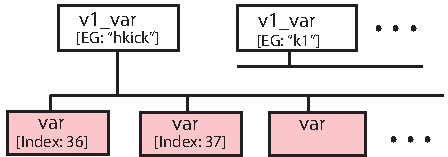
\includegraphics[width=4in]{var-tree.pdf}
  \caption[VAriable tree structure]
{A \vn{v1_var} structure holds an array of variables. Illustrated is a \vn{var_var} structure
holding an array of variables with each variable controlling the \vn{hkick} attribute of a
particular lattice element.}
  \label{f:var.tree}
\end{figure}

%-------------------------------------------------------------------------------

\index{variables!v1_var}
Blocks of variables are associated with what is called a \vn{v1_var} structure as illustrated in
Figure~\ref{f:var.tree}. Each \vn{v1_var} structure defined has a \vn{name} with which to refer to
in \tao commands. For example, if ``\vn{quad_k1}'' is the name of a \vn{v1_var}, then
\vn{quad_k1[5]} references the variable with index 5 in the array associated with the \vn{quad_k1}
\vn{v1_var} structure.

A set of variables within a \vn{v1_var} block can be referred to by using using a comma \vn{,} to
separate their indexes. Additionally, a Colon ``\vn{:}'' can be use to specify a range of
variables. For example
\begin{example}
  quad_k1[3:6,23]
\end{example}
refers to variables 3, 4, 5, 6, and 23. Instead of a number, the associated lattice element name can
be used so if, in the above example, the lattice element named \vn{q01} is associated with
\vn{quad_k1[1]}, etc., then the following is equivalent:
\begin{example}
  quad_k1[q03:q06,q23]
\end{example}
Using lattice names instead of numbers is not valid if the same lattice element is associated with
more than one variable in a \vn{v1_var} array. This can happen, for example, if one variable
controls an element's \vn{x_offset} and another variable controls the same element's \vn{y_offset}.

In referring to variables, a ``\vn{*}'' can be used as a wild card to 
denote ``all''. Thus:
\begin{example}
  *                 ! All the variables
  quad_k1[*]|design ! All design values of quad_k1.
  quad_k1[]|model   ! No values. That is, the empty set.
  quad_k1|model     ! Same as quad_k1[*]|model
\end{example}

%-------------------------------------------------------------------------------
\section{Anatomy of a Variable}
\label{s:var.anatomy}

A given variable may control a single parameter of one element (or \vn{particle_start}) in a
\vn{model} lattice of a single universe or it can be configured to simultaneously control an element
attribute across multiple universes. Any one variable cannot control more than one attribute of one
element. However, a variable may control an overlay or group element which, in turn, can control
numerous elements.

Each individual variable has a number of values associated with it: The list of components that can
be set or refereed to are:
\begin{example}
  ele_name     ! Associated lattice element name.
  attrib_name  ! Name of the attribute to vary.
  ix_attrib    ! Index in ele%value(:) array if appropriate.
  s            ! longitudinal position of ele.

  meas         ! Value of variable at time of a data measurement.
  ref          ! Value at time of the reference data measurement.
  model        ! Value in the model lattice.
  base         ! Value in the base lattice.
  design       ! Value in  the design lattice.
  correction   ! Value determined by a fit to correct the lattice.
  old          ! Scratch value.

  weight       ! Weight used in the merit function.
  delta_merit  ! Diff used to calculate the merit function term.
  merit        ! merit_term = weight * delta^2.
  merit_type   ! "target" or "limit"
  dMerit_dVar  ! Merit derivative.

  high_lim     ! High limit for the model_value.
  low_lim      ! Low limit for the model_value.
  step         ! For fitting/optimization: What is considered a small change.

  key_bound    ! Variable bound to keyboard key?
  ix_key_table ! Has a key binding?

  ix_v1        ! Index of this var in the s%v1_var(i)%v(:) array.
  ix_var       ! Index number of this var in the s%var(:) array.
  ix_dvar      ! Column in the dData_dVar derivative matrix.

  exists       ! Does the variable exist?
  good_var     ! The variable can be varied (set by \tao).
  good_user    ! The variable can be varied (set by the user).
  good_opt     ! For use by extension code.
  good_plot    ! Is variable within the horizontal extent of the plot? 
  useit_opt    ! Variable is to be used for optimizing.
  useit_plot   ! Variable is to be used for plotting.
\end{example}

  \index{variable!measured}\index{variable!reference}
  \index{variable!model}\index{variable!design}\index{variable!base}
  \begin{description}
  \item[attrib_name] \Newline
Name of the attribute to vary. Consult the \bmad manual for appropriate attribute names. If the
attribute is associated with a lattice element, the \vn{show element -all} command will list most
attributes of interest.  It is important to keep in mind that it is not possible to use attributes
that are computed (that is, dependent attributes).
  \item[base] \Newline
The value of the variable as derived from the \vn{base} lattice (\sref{s:universe}).
  \item[delta_merit] \Newline
Difference value used to calculate the contribution of the variable to the merit function (\Eq{m1}).
  \item[design] \Newline
The value of the variable as given in the \vn{design} lattice.
  \item[dMerit_dVar] \Newline
Derivative of the merit function with respect to the variable.
  \item[ele_name] \Newline
Associated lattice element name. For controlling the starting position in a lattice with open
geometry the element name is \vn{particle_start} (which is the name used if the starting position is
set in the lattice file). 
  \item[exists] \Newline
The variable exists. Non-existent variables can serve as place holders in a variable
array.
  \item[good_opt] \Newline
Logical not modified by Tao proper and reserved for use by extension code. See below.
  \item[good_plot] \Newline
Set by Tao. Is variable point within the horizontal extent of the plot? 
  \item[good_var] \Newline
Logical controlled by \tao and used to veto variables that should not be varied during
optimization. For example, variables that do not affect the merit function. See below.
  \item[good_user] \Newline
Logical set by the user using \vn{veto}, \vn{use}, and \vn{restore} commands to indicate
whether the variable should be used when optimizing. See below.
  \item[high_lim] \Newline
High limit for the model value during optimization (\sref{s:del.v}) beyond which
the contribution of the variable to the merit function is nonzero.
  \item[ix_attrib] \Newline
Index assigned by \bmad to the attribute being controlled. Used for diagnosis and not
of general interest.
  \item[ix_dvar] \Newline
Column index of the variable in the dData_dVar derivative matrix constructed by \tao.
Used for diagnostics and not of general interest.
  \item[ix_key_table] \Newline
Index of the variable in the key table (\sref{s:key.bind}).
  \item[ix_v1] \Newline
Index of this variable in the variable array of the associated \vn{v1_var} variable.
For example, a variable named \vn{q1_quad[10]} would have \vn{ix_v1} equal to 10.
  \item[ix_var] \Newline
For ease of computation, \tao establishes an array that holds all the variables.
\vn{ix_var} is the index number for this variable in this array. 
Used for diagnostics and not of general interest.
  \item[key_bound] \Newline
Variable bound to keyboard key (\sref{s:key.bind})?
  \item[measured] \Newline
The value of the variable as obtained at the time of a \vn{data} measurement.
  \item[merit] \Newline
The contribution to the merit function \Eq{m1} from the variable. Use the \vn{show merit}
command to set the variables and data which contribute most to the merit function.
  \item[merit_type] \Newline
"target" or "limit".
  \item[low_lim] \Newline
Lower limit for the model value during optimization (\sref{s:del.v}) beyond which
the contribution of the variable to the merit function is nonzero.
  \item[model] \Newline
The value of the variable as given in the \vn{model} lattice.
  \item[reference] \Newline
The Value of the variable as obtained at the time of a \vn{reference} data measurement
(\sref{s:lat.correction}).
  \item[s] \Newline
longitudinal position of element whose attribute the variable is controlling.  Since a
variable may control multipole attributes in multiple elements at different s-positions,
The value of \vn{s} may not be relevant.
  \item[step] \Newline
What is considered a small change in the variable but large enough to be able to compute
derivatives by changing the variable by \vn{step}. Used for fitting/optimization.  
  \item[useit_opt] \Newline
Variable is to be used for optimization. See below.
  \item[useit_plot] \Newline
If True, variable is used when plotting variable values. See below.
  \item[weight] \Newline
Weight used in the merit function. $w_j$ in \Eq{m1}
  \end{description}

These components and others can be refereed to in expressions using the notation documented
in \Sref{s:var.token}.

%-------------------------------------------------------------------------------
\section{Use in Optimization and Graphing}
\label{s:var.use}

Use the \vn{show var} (\sref{s:show}) command to see variable information

When using optimization for lattice correction or lattice design (\sref{c:opti}), Individual
variables can be excluded from the process using the \vn{veto} (\sref{s:veto}), \vn{restore}
(\sref{s:restore}), and \vn{use} (\sref{s:use}) commands. These set the \vn{good_user} component of
a variable. This, combined with the setting \vn{exists}, \vn{good_var}, and \vn{good_opt} determine
the setting of \vn{useit_opt} which is the component that determines if the datum is used in the
computation of the merit function.
\begin{example}
  useit_opt = exists \& good_user \& good_opt \& good_var
\end{example}
The settings of everything but \vn{good_user} and \vn{good_opt} is determined by \tao

For a given \vn{graph} that potentially will use a given variable for plotting, 
the \vn{useit_plot} component is set to True if the variable is actually used for plotting.
\vn{useit_plot} is set by \tao using the prescription:
\begin{example}
  useit_plot = exists \& good_plot \& good_var \& 
                            (good_user | graph:draw_only_good_user_data_or_vars)
\end{example}
Since \vn{useit_plot} is set on a graph by graph basis, If multipole graphs that use a particular
variable are to be plotted, The setting of \vn{useit_plot} at the end of plotting will just be
the setting for the last graph that was plotted.

%-------------------------------------------------------------------------------
\section{Slave Value Mismatch}
\label{s:var.mismatch}

A ``slave value mismatch'' happens when a variable is controlling multiple parameters and something
happens so that some subset of the controlled parameters have a change in value. For example, if a
lattice has multiple elements named \vn{``Q''}, and a variable controls the \vn{k1} attribute of all
of these elements, then, say, if only the value of \vn{k1} of element \vn{Q\#\#2} (the 2nd instance
of \vn{Q} in the lattice) is changed, there will be a slave value mismatch. This can happen with the
\vn{change element} or \vn{set element} command, and can also happen with the \vn{read lattice}
command.  Additionally, slave value mismatches can happen if there are multiple universes with
variables controlling parameters in more than one universe. In this case, modifying parameters in
only one universe can cause slave value mismatches.

\tao can fix slave value mismatches when the \vn{set element} or \vn{change element} commands by using
the changed parameter to set all the slave parameters. In other cases, \tao will not know what is changed
and will simply set all the slave values to the value of the first slave.

\chapter{Data}
\label{c:data}
\index{data|hyperbf}

A \tao \vn{``datum''} is a parameter associated with a lattice that is used in lattice correction or
design (\sref{c:opti}). Example data includes the vertical orbit at a particular position or the
horizontal emittance of a storage ring. This chapter explains how data is organized in \tao while
Section~\sref{s:init.data} explains how, in an initialization file, to define the structures that
hold the data.  When running \tao, the \vn{show data} (\sref{s:show}) command can be used to view
information about the data.

%------------------------------------------------------------------------
\section{Data Organization}
\label{s:data.org}

\begin{figure}
  \centering
  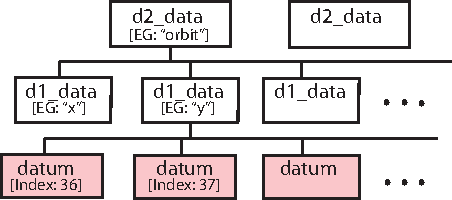
\includegraphics[width=4in]{data-tree.pdf}
  \caption[Data tree structure]
{A \vn{d2_data} structure holds a set of \vn{d1_data} structures. 
A \vn{d1_data} structure holds an array of datums.}
  \label{f:data.tree}
\end{figure}

\index{d2_data}\index{d1_data}
The horizontal orbit at a particular BPM is an example of an individual \vn{datum}. For ease of
manipulation, arrays of datums are grouped into what is called a \vn{d1_data}
structure. Furthermore, sets of \vn{d1_data} structures are grouped into what is called a
\vn{d2_data} structure.  This is illustrated in Figure~\ref{f:data.tree}.  For example, a
\vn{d2_data} structure for orbit data could contain two \vn{d1_data} structures --- one \vn{d1_data}
structure for the horizontal orbit data and another \vn{d1_data} structure for the vertical orbit
data. Each datum of, say, the horizontal orbit \vn{d1_data} structure would then correspond to the
horizontal orbit at some point in the machine. 

When issuing \tao commands, all the data associated with a \vn{d2_data} structure is specified using
the \vn{d2_data} structure's \vn{name}.  The data associated with a \vn{d1_data} structure is
specified using the format
\begin{example}
  d2_name.d1_name
\end{example}
For example, if a \vn{d2_data} structure has the name ``\vn{orbit}'', and one of its \vn{d1_data}
structures has the name ``\vn{x}'', then \tao commands that refer to the data in this \vn{d1_data}
structure use the name ``\vn{orbit.x}''. Sometimes there is only one \vn{d1_data} structure for a
given \vn{d2_data} structure. In this case the data can be referred to simply by using the
\vn{d2_data} structure's name. The individual datums can be referred to using the notation
\begin{example}
  <d2_name>.<d1_name>[<list_of_datum_indexes>]
\end{example}
For example, \vn{orbit.x[10]} refers to the horizontal orbit datum with index 10. Notice that the
beginning (lowest) datum index is user selectable and is therefore not necessarily 1.

Period characters are not allowed in both the \vn{d2_data} and \vn{d1_data} names.

It is important to note that the name given to \vn{d2_data} and \vn{d1_data} structures is arbitrary
and does not have to correspond to the type of data contained in the structures. In fact, a
\vn{d1_data} array can contain heterogeneous data types.  Thus, for example, it is perfectly
permissible (but definitely not recommended) to set up the data structures so that, say,
\vn{orbit.x[10]} is the $a$-mode emittance at a certain element and \vn{orbit.x[11]} is the $b$-mode
beta function at the same element.

Ranges of data can be referred to using using a comma \vn{,} to separate the indexes combined with
the notation \vn{n1:n2} to specify all the datums between \vn{n1} and \vn{n2} inclusive. For example
\begin{example}
  orbit.x[3:6,23]
\end{example}
refers to datums 3, 4, 5, 6, and 23. 

If multiple universes are present, each universe will have its own set of \vn{d2_data}
structures. The name of a particular \vn{d2_data} structure may be the same as a \vn{d2_data}
structure in a separate universe. So, for example, an \vn{orbit} \vn{d2_data} structure may
be present in multiple universes.

As explained in \sref{s:universe}, the prefix \vn{"@"} may
be used to specify which universe the data applies to. The general notation is
\begin{example}
  [<universe_range>]@<d2_name>.<d1_name>[<datum_index>]
\end{example}
Examples:
\begin{example}
  [2:4,7]@orbit.x ! The \vn{orbit.x} data in universes 2, 3, 4 and 7.
  [2]@orbit.x     ! The \vn{orbit.x} data in universe 2. 
  2@orbit.x       ! Same as "2@orbit.x".
  orbit.x         ! The \vn{orbit.x} data in the current default universe.
  -1@orbit.x      ! Same as "orbit.x".
\end{example}

As explained in Section~\sref{s:data.anatomy}, each individual datum has a number of components. The
syntax to refer to a component is:
\begin{example}
  d2_name.d1_name[datum_index]|component
\end{example}
For example:
\begin{example}
  orbit.x[3:10]|meas     ! The measured data values
\end{example}

In referring to datums, a ``\vn{*}'' can be used as a wild card to 
denote ``all''. Thus:
\begin{example}
  *@orbit.x       ! The \vn{orbit.x} data in all universes.
  *               ! All the data in the current default universe.
  *.*             ! Same as "*"
  *@*             ! All the data in all the universes. 
  *@*.*           ! Same as "*@*"
  orbit.x[*]|meas ! All measured values of orbit.x
  orbit.x[]|meas  ! No values. That is, the empty set.
  orbit.x|meas    ! Same as orbit.x[*]|meas.
\end{example}
The last example shows that when referring to an entire block of data
encompassed by a \vn{d1_data} structure, the \vn{[*]} can be omitted.

%------------------------------------------------------------------------
\section{Anatomy of a Datum}
\label{s:data.anatomy}

Each datum has a number of components associated with it:
\begin{example}
  data_type       ! Character: Type of data: "orbit.x", etc.
  ele_name        ! Character: Name of lattice element where datum is evaluated at.
  ele_start_name  ! Character: Name of starting lattice element in a range.
  ele_ref_name    ! Character: Name of reference lattice element.
  merit_type      ! Character: Type of constraint: "target", "max", etc.
  data_source     ! Character: How the datum is calculated. "lat", "beam", etc.
  ix_ele\Ss         ! Integer: Index of "ele" in the lattice element list.
  ix_branch\Ss      ! Integer: Lattice branch index.
  ix_ele_start\Ss   ! Integer: Index of "ele_start" in the lattice element list.
  ix_ele_ref\Ss     ! Integer: Index of "ele_ref" in the lattice element list.
  ix_ele_merit\Ss   ! Integer: Lattice index where merit is evaluated.
  ix_d1\Ss          ! Integer: Index number in d1_data structure
  ix_data\Ss        ! Integer: Index in the global data array
  ix_dModel\Ss      ! Integer: Row number in the dModel_dVar derivative matrix.
  ix_bunch        ! Integer: Bunch number to get the data from.
  eval_point      ! Character/integer: Evaluation point relative to the lattice element.
  meas            ! Real: User set measured datum value.
  ref             ! Real: User set measured datum value from the reference data set.
  model\Ss          ! Real: Datum value as calculated from the model.
  design\Ss         ! Real: What the datum value is in the design lattice.
  old\Ss            ! Real: Used by \tao to save the model at some previous time.
  base\Ss           ! Real: The value as calculated from the base model.
  fit\Dd            ! Real: This value is not used by \tao.
  invalid         ! Real: The value used for delta_merit if good_model = False.
  error_rms       ! Real: Measurement error. Used for plotting.
  delta_merit\Ss    ! Real: Diff used to calculate the merit function term.
  weight          ! Real: Weight for the merit function term
  merit\Ss          ! Real: Merit function term value: weight * delta^2
  s\Ss              ! Real: longitudinal position of ele.
  s_offset        ! Real: Offset of the evaluation point.
  spin_axis       ! Structure: Used for Spin G-matrix calculations.
  exists\Ss         ! Logical: Does the datum exist?
  good_model\Ss     ! Logical: Does the model  component contain a valid value?
  good_design\Ss    ! Logical: Does the design component contain a valid value?
  good_base\Ss      ! Logical: Does the base   component contain a valid value?
  good_meas       ! Logical: Does the meas   component contain a valid value?
  good_ref        ! Logical: Does the ref    component contain a valid value?
  good_user       ! Logical: Does the user want this datum used in optimization?
  good_opt\Dd       ! Logical: Similar to good_user. Can be used in Tao extensions.
  good_plot\Dd      ! Logical: Is datum within the horizontal extent of the plot?
  useit_plot\Ss     ! Logical: Is this datum to be used in plotting?
  useit_opt\Ss      ! Logical: Is this datum to be used for optimization?
\end{example}
\Ss Set by \tao. \Dd Used by \tao extensions. Not user settable.

When running \tao, the \vn{show data} (\sref{s:show}) command can be used to view the components of a datum. 
The \vn{set} command (\sref{s:set}) can be used to set some of these components.
Note: Some of these components are set by the user and some of these components will be calculated by
\tao. A description of what components can be set is given in \Sref{s:init.data}.

\begin{description}
  \item[base] \Newline
The value of the datum as calculated from the base lattice (\sref{s:datum.values}).
%
  \item[data_source] \Newline
The \vn{data_source} component specifies where the data is coming from
(\sref{s:data.source}).
%
  \item[data_type] \Newline
The type of data (\sref{s:data.types}). For example, \vn{beta.a}. At startup, if the
\vn{data_type} is not specified, it is set to \vn{<d2_name>.<d1_name>} where
\vn{<d2_name>} is the name of the associated \vn{d2} data structure and \vn{<d1_name>} is 
the name of the associated \vn{d1} data structure (\sref{s:init.data}).
%
  \item[delta_merit] \Newline
Difference used to calculate the contribution of the datum to the merit function (\sref{s:lat.correction}).
%
  \item[design] \Newline
The value of the datum as calculated from the design lattice (\sref{s:datum.values}).
%
  \item[ele_name] \Newline
Name of the associated lattice element where the datum is evaluated at (\sref{s:data.lat.ele}) or,
if \vn{ele_start_name} is set, the last element in the evaluation range. Not used for datums that
are \vn{global}, like the emittance. Also see \vn{eval_point} and \vn{s_offset} components.
%
  \item[ele_start_name] \Newline
Starting element of a range of lattice elements (\sref{s:data.lat.ele}).
%
  \item[ele_ref_name] \Newline
Reference lattice element (\sref{s:data.lat.ele}). Not to be confused with the \vn{ref} component
which is a user settable value.
%
  \item[error_rms] \Newline
The error associated with the measured or reference data values. Used for drawing error bars. See the 
documentation on \vn{curve(N)%draw_error_bars} in \Sref{s:template}.
for more details.
%
  \item[eval_point] \Newline
Set to "\vn{beginning}", "\vn{center}", or "\vn{end}". Used with \vn{s_offset} to determine where
the datum is evaluated at (\sref{s:dat.eval}). The evaluation point will be ignored if using an
evaluation range (\vn{ele_start_name} is set) is used.
%
  \item[exists] \Newline
Set by \tao to True if the datum exists (\sref{s:datum.opt}). 
%
  \item[fit] \Newline
Not used by \tao. Can be used with custom code.
%
  \item[good_base] \Newline
Set by \tao. Is the \vn{base} value valid?
%
  \item[good_design] \Newline
Set by \tao. Is the value as calculated from the \vn{design} lattice valid? For example, if the
datum is the particle orbit at some BPM in a ring and if it is not possible to compute the orbit at
the BPM due to the lattice being unstable then \vn{good_design} will be False.
%
  \item[good_meas] \Newline
Set by \tao. Is the \vn{meas} value valid?
%
  \item[good_model] \Newline
Set by the user. Is the value as calculated from the \vn{model} lattice valid? For example, if the
datum is the particle orbit at some BPM in a lattice with open geometry and if it is not possible to
compute the orbit at the BPM due to the particle being lost upstream of the element then
\vn{good_model} will be False.
%
  \item[good_opt] \Newline
Set by the user. This component is similar \vn{good_user} except that it is unaffected by the
\vn{veto}, \vn{restore} and \vn{use} commands.
%
  \item[good_plot] \Newline
Set by Tao. Is datum within the horizontal extent of the plot? 
%
  \item[good_ref] \Newline
Set by the user. Is the \vn{ref} value valid?
%
  \item[good_user] \Newline
Set by the user. Is the datum valid for optimization or plotting? Use the commands \vn{veto}, \vn{restore},
\vn{use} and \vn{set data} to set while running \tao.
%
  \item[invalid] \Newline
The value used in the computation of \vn{delta_merit} one of the following three conditions is
True: 1) if \vn{good_model} = False, or 2) if \vn{good_base} is False when the global \vn{opt_with_base}
is True, or 3) if \vn{good_design} is False when the global \vn{opt_with_ref} is True.
%
  \item[ix_branch] \Newline
The index of the lattice branch that contains \vn{ele}, \vn{ref_ele}, and \vn{start_ele}.
%
  \item[ix_ele] \Newline
Index of the lattice element where the datum is evaluated at. 
%
  \item[ix_ele_start] \Newline
Index of the start element.
%
  \item[ix_ele_ref] \Newline
Index of the reference element.
%
  \item[ix_ele_merit] \Newline
Set by \tao. When the \vn{merit_type} is set to \vn{max} or \vn{min} and there is a range
of elements that over which the there is an evaluation, ix_ele_merit is set to the element
where the value is the \vn{max} or \vn{min}.
%
  \item[ix_d1] \Newline
Index of the associated \vn{d1_data} array.
%
  \item[ix_data] \Newline
For convenience, all the datums of a given universe are put into one large array. \vn{ix_data} is the index
of the datum in this array. This is useful for debugging purposes.
%
  \item[ix_dModel] \Newline
For optimization, \tao creates a derivative matrix dMerit_i/dVar_j. \vn{ix_dmodel} is set
to the i\Th column of this matrix. This is useful for debugging purposes
%
  \item[ix_bunch] \Newline
For datums that have \vn{data_source} set to \vn{beam}, \vn{ix_bunch} selects which bunch
of the beam the datum is evaluated at.
%
  \item[meas] \Newline
The value of the datum as obtained from some measurement (\sref{s:datum.values}).
%
  \item[merit] \Newline
The contribution to the merit function due to this datum (\sref{s:lat.correction}).
%
  \item[merit_type] \Newline
The type of merit (\sref{s:del.d}). Possible values are:
\begin{example}
  "target"
  "min",     "max"
  "abs_min", "abs_max"
  "max-min"                     ! Only used when datum specifies a range of elements.
  "average", "integral", "rms"  ! Only used when datum specifies a range of elements.
\end{example}
%
  \item[model] \Newline
The value of the datum as calculated from the \vn{model} lattice (\sref{s:datum.values}).
%
  \item[old] \Newline
A datum value that was saved at some point in \tao's calculations. This value
can be ignored (\sref{s:datum.values}).
%
  \item[ref] \Newline
The reference datum value as obtained from some reference measurement (\sref{s:datum.values}).
Set by the User. Not to be confused with the reference element.
%
  \item[s] \Newline
Longitudinal $s$-position of the lattice element.
%
  \item[s_offset] \Newline
Offset of the evaluation point when there is an associated lattice element (\sref{s:dat.eval}).
The offset will be ignored if using an evaluation range (\vn{ele_start_name} is set) is used.
%
  \item[spin_axis]
The \vn{spin_axis} component is a structure used for Spin G-matrix calculations
(\vn{spin_g_matrix.$ij$} data type). \vn{Spin_axis} gives the $(l, n_0, m)$ coordinate axes at the
reference element. See \sref{s:init.data} for documentation on how to set this structure.
%
  \item[useit_opt] \Newline
Datum is used for optimization. \vn{useit_opt} is set by \tao using the other
\vn{logicals} components using the prescription:
\begin{example}
  useit_opt = exists \& useit_opt \& good_user \& good_meas \& 
              good_ref (if reference data is used in optimization)
Notice that if, for example, \vn{good_model} is False then the datum will still be used for optimization but
in this case the \vn{invalid} value set by the user will be used in the computation for \vn{delta_merit} in
place of a value computed from lattice.
\end{example}
%
%
  \item[useit_plot] \Newline
Set \vn{True} if the datum is valid for plotting for a particular graph. This component gets
reevaluated for each \vn{graph} that potentially uses the datum so the value observed after plotting is
refreshed is simply the value as calculated for the last \vn{graph} considered. The value for \vn{useit_plot}
is evaluated using other logical components using the prescription:
\begin{example}
  useit_plot = exists \& good_plot \& 
                  (good_user | graph:draw_only_good_user_data_or_vars) \&
                  good_meas (if measured data is being plotted) \& 
                  good_ref (if reference data is being plotted) \&
                  good_model (if model data is being plotted)
\end{example}
%
  \item[weight] \Newline
Weight used in evaluating the contribution of the datum to the merit function (\sref{s:lat.correction}).
\end{description}

%------------------------------------------------------------------------
\section{Datum values}
\label{s:datum.values}

\index{data!measured}\index{data!reference}\index{data!model}
\index{data!base}\index{data!design}
A given datum has six values associated it:
\vspace{-2ex}
\begin{description}
  \vspace{-1ex}
  \item[meas] \Newline 
When fitting data, the \vn{meas} value is the value of the datum as obtained from some
measurement. When designing lattices, the \vn{meas} value is the desired value of the datum. For
example, when designing a lattice for a colliding ring machine, a datum may be constructed for 
the beta function at the interaction point with the \vn{meas} value set to the desired value. See
Chapter~\ref{c:opti} for more details.
  \vspace{-1ex}
  \item[base] \Newline
The datum value as calculated from the \vn{base} lattice (\sref{s:lattice}).
  \vspace{-0.5ex}
  \item[design] \Newline
The value of the datum as calculated from the \vn{design} lattice (\sref{s:lattice}).
  \vspace{-0.5ex}
  \item[fit] \Newline
The \vn{fit} value is not used by \tao directly and is available for use by custom code.
  \vspace{-0.5ex}
  \item[model] \Newline
The value of the datum as calculated from the \vn{model} lattice (\sref{s:lattice}).
  \vspace{-0.5ex}
  \item[old] \Newline
A datum value that was saved at some point in \tao's calculations. This value
can be ignored.
  \vspace{-0.5ex}
  \item[ref] \Newline
When fitting data, \vn{ref} is the datum value as obtained from some reference measurement. For
example, a measurement before some variable is varied could be designated as the \vn{reference}, and
the datum taken after the variation could be designated the \vn{measured} datum. When designing
lattices, the \vn{ref} value is the value of the datum associated with the \vn{design} or \vn{base}
lattice (determined by the setting of the global \vn{opt_with_base} parameter
(\sref{s:del.d}). Note: The \vn{meas} value of a datum is always associated with the
\vn{model} lattice.
\end{description}

%------------------------------------------------------------------------
\section{Evaluation Point of a Datum}.
\label{s:dat.eval}

When the datum is to be evaluated at a specific point in the lattice, that is, when there
is an associated lattice element, the default position for evaluating the datum is at the
downstream end of the element. This evaluation point can be shifted using the
\vn{eval_point} and/or \vn{s_offset} components. 

The \vn{eval_point} component can be set to one of:
\begin{example}
  beginning   ! entrance end of lattice element.
  center      ! Center of lattice element
  end         ! Exit end of lattice element. Default.
\end{example}
The evaluation point is shifted by \vn{s_offset} from the \vn{eval_point}.

If there is a reference point, the setting of \vn{eval_point} is used to determine where
the reference point. The setting of \vn{s_offset} is ignored for the reference point.

Due to internal logic considerations, Not all \vn{data_type}s are compatible with a finite
\vn{s_offset} or a setting of \vn{eval_point} to \vn{center}. The table of \vn{data_type}s
(\sref{t:data.types}) shows which \vn{data_type}s are compatible and which are not.

Another restriction is that specifying a range of elements for evaluation (that is,
specifying \vn{ele_start_name} \sref{s:init.data}) is not compatible with a finite
\vn{s_offset} or a setting of \vn{eval_point} to \vn{center}.

%------------------------------------------------------------------------
\section{Datums in Optimization}
\label{s:datum.opt}

When using optimization for lattice correction or lattice design (\sref{c:opti}), Individual datums
can be excluded from the process using the \vn{veto} (\sref{s:veto}), \vn{restore}
(\sref{s:restore}), and \vn{use} (\sref{s:use}) commands. These set the \vn{good_user} component of
a datum. This, combined with the setting \vn{exists}, \vn{good_meas}, \vn{good_ref}, and
\vn{good_opt} determine the setting of \vn{useit_opt} which is the component that determines if the
datum is used in the computation of the merit function. The settings of everything but
\vn{good_user} is determined by \tao. The value of \vn{good_user} for a datum can be set in an
initialization file (\sref{s:init.data}) or on the command line using the \vn{use}, (\sref{s:use})
\vn{veto} (\sref{s:veto}), or \vn{restore} (\sref{s:restore}) commands.

The \vn{exists} component is set by \tao to True if the datum exists and False otherwise. A datum
may not exist if the type of datum requires the designation of an associated element but the
\vn{ele_name} component is blank. For example, a \vn{d1_data} array set up to hold orbit data may
use a numbering scheme that fits the lattice so that , say, datum number 34 in the array does not
correspond to an existing BPM.

The \vn{good_model} component is set according to whether a datum value can be computed from the
\vn{model} lattice. For example, If a circular lattice is unstable, the beta function and the closed
orbit cannot be computed. Similarly, the \vn{good_design} and \vn{good_base} components mark whether
the \vn{design} and \vn{base} values respectively are valid.

The \vn{delta_merit} component of a datum is set to the \vn{delta} value used in computing the
contribution to the merit function (\sref{s:del.d}). If it is not possible to compute
the datum value, then the \vn{invalid} component is used for the computation of \vn{delta_merit}.
It is not possible to compute the datum value if one of the following three conditions is True: 1)
\vn{good_model} is False, 2) \vn{good_design} is False and the global \vn{opt_with_ref} is True, or
3) \vn{good_base} is False and the global \vn{opt_with_base} is True.

\vn{good_meas} is set True if the \vn{meas} component value is set in the data initialization file
(\sref{s:init.data}) or is set using the \vn{set} command (\sref{s:set}). Similarly, \vn{good_ref}
is set True if the \vn{ref} component has been set. \vn{good_ref} only affects the setting of
\vn{useit_opt} if the optimization is using reference data as set by the global variable
\vn{opt_with_ref} (\sref{s:globals}).

Finally \vn{good_opt} is meant for use in custom versions of \tao (\sref{c:custom.tao}) and is
always left True by the standard \tao code.

Example of using a \vn{show data} (\sref{s:show}) to check the logicals
in a datum:
\begin{example}
  Tao> show data 3@beta[1]

  Universe:   3
  %ele_name          = IP_L0
  %ele_ref_name      =
  %ele_start_name    =
  %data_type         = beta.a
      ... etc ...
  %exists            =  T
  %good_model        =  T
  %good_meas         =  F
  %good_ref          =  F
  %good_user         =  T
  %good_opt          =  T
  %good_plot         =  F
  %useit_plot        =  F
  %useit_opt         =  F
\end{example}
Here \vn{useit_opt} is False since \vn{good_meas} is False and \vn{good_meas} is False since the
\vn{meas} value of the datum (not shown) was not set in the \tao initialization file or set using
the \vn{set} command.

%------------------------------------------------------------------------
\section{Data_source}
\index{data!data_source}
\label{s:data.source}

The \vn{data_source} component specifies where the data is 
coming from. Possible values are:
\begin{example}
  "beam"        ! Data from from multiparticle beam distribution
  "data"        ! Data from from a \tao datum in a data array.
  "lat"         ! Data from from the lattice.
\end{example}
If \vn{data_source} is set to \vn{"beam"}, the data is calculated
using multiparticle tracking.  If \vn{data_source} is set to
\vn{"lat"}, the data is calculated using the ``lattice'' which here
means everything {\em but} multiparticle tracking In particular, the "\vn{lat}" \vn{data_source}
includes data derived from single particle tracking. For example, the
\vn{"beam"} based calculation of the emittance uses the bunch sigma
matrix obtained through multiparticle tracking. The \vn{"lat"} based
calculation of the emittance uses radiation integrals.

Some data types may be restricted as to which \vn{data_source} is
possible. For example, a datum with \vn{data_type} set to
\vn{n_particle_loss} must use \vn{"beam"} for the \vn{data_source}. 
Table~\ref{t:data.types} lists which \vn{data_source} values are valid
for what data types.

%------------------------------------------------------------------------
\section{Datum Evaluation and Associated Lattice Elements}
\index{data!associated lattice elements}
\label{s:data.lat.ele}

Datums can be divided up into two classes. In one class are the datums
that are \vn{``local''}, like the beam orbit, which need to be evaluated at
either a particular point are evaluated over some finite region of the
machine. Other datums, like the emittance, are \vn{``global''} and do not
have associated evaluation points.

As mentioned, \vn{local} datums may be evaluated at a specific point
or over some evaluation region, an evaluation region is used when, for
example, the maximum or minimum value over a region is wanted. To
specify an evaluation point, an \vn{evaluation element} must be
associated with a datum. The evaluation point will be at the exit end
of this element. To specify an evaluation region, a \vn{start element}
must also be associated with a datum along with the \vn{evaluation
element}. The evaluation region is from the exit end of the \vn{start
element} to the exit end of the \vn{evaluation element}.

In addition to the \vn{evaluation element} and the \vn{start element}, a \vn{local} datum may have
an associated \vn{reference element}.  A \vn{reference element} is used as a fiducial point and the
datum value is calculated relative to that point. For example, a datum value may be the position of
the \vn{evaluation element} relative to the position of the \vn{reference element}. The evaluation
point of a \vn{reference element} is the exit end of that element.

The components in a datum corresponding to the \vn{evaluation element}, the \vn{reference element},
and the \vn{start element}.  are shown in Table~\ref{t:datum.elements}.  These three elements may be
specified for a datum by either setting the name component or the index component of the
datum. Using the element index over the element name is necessary when more than one element in the
lattice has the same name.

\begin{table}[htb]
\centering
\begin{tabular}{lll}
  \toprule
  &\multicolumn{2}{c}{\it Data Component} \\ \cmidrule{2-3}
  {\it Element} & {\it name} & {\it index} \\ \midrule
  Reference Element  & \vn{ele_ref_name}   & \vn{ix_ele_ref}   \\
  Start Element      & \vn{ele_start_name} & \vn{ix_ele_start} \\
  Evaluation Element & \vn{ele_name}       & \vn{ix_ele}       \\ \bottomrule
\end{tabular}
\caption[The three lattice elements associated with a datum.]  {The three lattice elements
associated with a datum may be specified in the datum by setting the appropriate name component or
by setting the appropriate index component.}  \label{t:datum.elements}
\end{table}

If a datum has an associated \vn{evaluation} element, but no associated \vn{start} or \vn{reference}
elements, the \vn{model} value of that datum is the value of the \vn{data_type} at the
\vn{evaluation} element. For example, if a datum has:
\begin{example}
  data_type      = "orbit.x"
  ele_name       = "q12"
\end{example}
here the \vn{model} value of this datum will be the horizontal orbit at the element with name
\vn{q12}.

If a datum has an associated \vn{start} element, specified by either setting the \vn{ele_start_name}
or \vn{ix_ele_start} datum components, the datum is evaluated over a region from the exit end of the
\vn{start} element to the exit end of \vn{evaluation} element. For example, if a datum has:
\begin{example}
  data_type      = "beta.a"
  ele_name       = "q12"
  ele_start_name = "q45"
  merit_type     = "max"
\end{example}
then the \vn{model} value of this datum will be the maximum value of the a-mode beta function in the
\vn{model} lattice in the region from the exit end of the element with name \vn{q12} to the exit end
of the element with name \vn{q45}. The \vn{base} and \vn{design} values are computed similarly using
the \vn{base} and \vn{design} lattices. 

If the lattice branch associated with the datum has a closed geometry, and if the lattice element
associated with \vn{ele_start_name} is after the element specified by \vn{ele_name}, the evaluation
region will be the region from \vn{ele_start_name} to the end of the branch along with the region
from the beginning of the branch to the element specified by \vn{ele_name}. That is, the evaluation
region ``wraps'' around the end of the lattice.  

It does not make sense to specify an evaluation range when the datum's \vn{merit_type} is set to
\vn{"target"}. In this case, the \vn{model}, \vn{base}, and \vn{design} values are the value of the
datum at the evaluation element. Also notice that for datums that do not have an evaluation element,
for example, if \vn{data_type} is set to \vn{"emit.a"}, specifying an evaluation range does not make
sense.

Typically, in evaluating a datum over some region to find the maximum or minimum, \tao will only
evaluate the datum at the ends of the elements with the assumption that this is good enough. If this
is not good enough, marker elements can be inserted into the lattice at locations that matter. For
example, the maximum or minimum of the beta function typically occurs near the middle of a
quadrupole so inserting marker elements in the middle of quadrupoles will improve the accuracy of
finding the extremum beta.

If a datum has an associated \vn{reference} element, specified by either setting the
\vn{ele_ref_name} or \vn{ix_ele_ref} datum components, the \vn{model} value of the datum is the
value at the \vn{evaluation} element (or the value over the range \vn{ele_start} to the
\vn{evaluation} element if \vn{ele_start} is specified), minus the \vn{model} value at
\vn{ele_ref}. For example, if a datum has:
\begin{example}
  data_type      = "beta.a"
  ele_name       = "q12"
  ele_start_name = "q45"
  ele_ref_name   = "q1"
  merit_type     = "max"
\end{example}
then the \vn{model} value of the datum will be the same as the previous example minus the value of
the a-mode beta function at the exit end of element \vn{q1}. There are a number of exceptions to the
above rule and datum types treat the \vn{reference} element in a different manner. For example, the
\vn{r.} data type uses the \vn{reference} element as the starting point in constructing a transfer
matrix.

Do not confuse the \vn{ele_ref_name} component (see preceding paragraph) with the \vn{ref}
component. The \vn{ref} component is set by the User and typically represents the measured value of
the datum. For example, if two orbit measurements are made, the \vn{meas} component of a datum can
be set to the measured orbit for one of the measurements while the \vn{ref} component can be set to
the measured orbit for the other measurement. This way orbit differences can be analyzed.

%------------------------------------------------------------------------
\section{Data Types Table}
\label{s:data.table}

This section lists in table form all the data types defined by \tao and section~\sref{s:data.types}
describes in detail these data types.

\index{data!calculation method}
\index{unstable.orbit}\index{beta}\index{alpha}\index{eta}\index{eta}
\index{etap}\index{phase}\index{orbit}\index{wire}\index{building wall}\index{spin}
\index{cbar}\index{coupling}\index{floor}\index{r}\index{t}\index{tt}
\index{rad_int.i5a_e6}\index{rad_int.i5b_e6}\index{s_position}\index{e_tot}
\index{emittance}\index{chrom}\index{norm_emittance}
\index{sigma}\index{dpx_dx}\index{dpy_dy}\index{dpz_dz}\index{dpa_da}
\index{dpb_db}\index{rad_int.i1}\index{rad_int.i2}\index{rad_int.i2_e4}
\index{rad_int.i3}\index{rad_int.i3_e7}

%----------------------------------------------------------------------------------------------

{\tt\small
\begin{longtable}{lllll} 
  \caption{Predefined Data Types in Tao}
  \label{t:data.types}
  \\ \hline

  {\it Pg}{\texttt \#}    & {\it Data_Type}                      & {\it Description}   & {\it data_source} & 
                                            \begin{sideways} \parbox{0.6in}{\begin{tabular}{@{}l}
                                            {\it Can use} \\ {\it s_offset?} \end{tabular}} \end{sideways} \\ \hline\hline
  \endfirsthead

  \caption[]{(continued)} \\ \hline
  {\it Pg}{\texttt \#}    & {\it Data_Type}                      & {\it Description}   & {\it data_source} & 
                                            \begin{sideways} \parbox{0.6in}{\begin{tabular}{@{}l}
                                            {\it Can use} \\ {\it s_offset?} \end{tabular}} \end{sideways} \\ \hline\hline
  \endhead

  \pref{alpha}            & alpha.a, .b                         & Normal-Mode alpha function                & lat         & Yes \\ \hline 
  \pref{apparent.emit}    & apparent_emit.x, .y                 & Apparent emittance                        & lat, beam   & No  \\ \hline
  \pref{beta.a}           & beta.a, .b, .c                      & Normal-mode beta function                 & lat, beam   & Yes \\ \hline 
  \pref{beta.x}           & beta.x, .y, .z                      & Projected beta function                   & beam        & No  \\ \hline 
  \pref{bpm.cbar}         & \begin{tabular}{@{}l}   
                              bpm_cbar.22a, .12a, \\
                              \hspace{4em} .11b, .12b
                            \end{tabular}                       & Measured coupling                         & lat         & Yes \\ \hline
  \pref{bpm.eta}          & bpm_eta.x, .y                       & Measured dispersion                       & lat         & Yes \\ \hline
  \pref{bpm.orbit}        & bpm_orbit.x, .y                     & Measured orbit                            & lat, beam   & Yes \\ \hline
  \pref{bpm.phase}        & bpm_phase.a, .b                     & Measured betatron phase                   & lat         & Yes \\ \hline
  \pref{bpm.k}            & \begin{tabular}{@{}l}   
                              bpm_k.22a, .12a, \\
                              \hspace{4em} .11b, .12b   
                             \end{tabular}                      & Measured coupling                         & lat         & Yes \\ \hline
  \pref{bunch.charge}     & \begin{tabular}{@{}l}   
                              bunch_charge.live, \\
                              \hspace{4em} .live_relative
                            \end{tabular}                       & Charge of live particles                  & beam        & No  \\ \hline
  \pref{bunch.max}        & \begin{tabular}{@{}l}   
                              bunch_max.x, .y, .z, \\ 
                              \hspace{4em} .px, .py, .pz  
                            \end{tabular}                       & Max relative to centroid                  & beam        & No  \\ \hline
  \pref{bunch.min}        & \begin{tabular}{@{}l}
                              bunch_min.x, .y, .z, \\ 
                              \hspace{4em} .px, .py, .pz
                            \end{tabular}                       & Min relative to centroid                  & beam        & No  \\ \hline
  \pref{cmat}             & cmat.11, .12, .21, .22              & Coupling matrix elements                  & lat         & Yes \\ \hline 
  \pref{cmat}             & cbar.11, .12, .21, .22              & Normalized coupling matrix                & lat         & Yes \\ \hline 
  \pref{chrom.a}          & chrom.a, .b                         & Chromaticities for a ring                 & lat         & No  \\ \hline
  \pref{chrom.dbeta}      & chrom.dbeta.a, .dbeta.b             & Normalized Chromatic beta                 & lat         & No  \\ \hline
  \pref{chrom.deta}       & chrom.deta.x, .deta.y               & Chromatic dispersions                     & lat         & No  \\ \hline
  \pref{chrom.detap}      & chrom.detap.x, .detap.y             & Chromatic dispersion slopes               & lat         & No  \\ \hline
  \pref{chrom.dphi}       & chrom.dphi.a, .dphi.b               & Chromatic betatron phase                  & lat         & No  \\ \hline
  \pref{chrom.w}          & chrom.w.a, .w.b                     & Chromatic W-functions                     & lat         & No  \\ \hline
  \pref{chrom.ptc}        & \begin{tabular}{@{}l}
                              chrom_ptc.a.$N$, \\
                              chrom_ptc.b.$N$, \\
                              \hspace{4em} $N = 0, 1, \ldots$
                            \end{tabular}                       & Chromaticity Taylor terms                 & lat         & no  \\ \hline
  \pref{curly.h}          & curly_h.a, .b                       & \begin{tabular}{@{}l}
                                                                    Radiation integrals \\
                                                                    curly H function 
                                                                  \end{tabular}                             & lat         & Yes \\ \hline
  \pref{damp}             & damp.j_a, .j_b, .j_z                & Damping partition number                  & lat         & No  \\ \hline
  \pref{deta.ds.a}        & deta_ds.a, .b                       & Dispersion derivatives                    & lat         & Yes \\ \hline
  \pref{deta.ds.x}        & deta_ds.x, .y                       & Dispersion derivatives                    & lat         & Yes \\ \hline
  \pref{dpx.dx}           & dpx_dx, dpx_dy, etc.                & Bunch <x px> / <$x^2$> \& Etc...          & beam        & No  \\ \hline 
  \pref{da}               & \begin{tabular}{@{}l}
                              dynamic_aperture.$N$, \\
                              \hspace{4em} $N = 1, 2, 3 \ldots$
                            \end{tabular}                       & Dynamic aperture                          & lat         & No  \\ \hline
  \pref{e.tot.ref}        & e_tot_ref                           & Lattice reference energy (eV)             & lat         & No  \\ \hline
  \pref{element.attrib}   & element_attrib.<attr_name>          & lattice element attribute                 & lat         & No  \\ \hline
  \pref{emit.a}           & emit.a, .b, .c                      & Emittance                                 & lat, beam   & No  \\ \hline
  \pref{emit.x}           & emit.x, .y, .z                      & Projected emittance                       & lat, beam   & No  \\ \hline
  \pref{eta.x}            & eta.x, .y, .z                       & Dispersions                               & lat, beam   & Yes \\ \hline 
  \pref{eta.a}            & eta.a, .b                           & Normal-mode dispersions                   & lat, beam   & Yes \\ \hline 
  \pref{etap.x}           & etap.x, .y                          & Momentum dispersions                      & lat, beam   & Yes \\ \hline 
  \pref{etap.a}           & etap.a, .b                          & Momentum dispersions                      & lat, beam   & Yes \\ \hline 
  \pref{expression}       & expression:<expression>             & See text above                            & lat         & No  \\ \hline 
  \pref{floor}            & \begin{tabular}{@{}l}   
                              floor.x, .y, .z, \\             
                              \hspace{2em} theta, .phi, .psi
                            \end{tabular}                       & \begin{tabular}{@{}l}   
                                                                    Lattice element \\
                                                                    global position
                                                                   \end{tabular}                            & lat         & Yes \\ \hline
  \pref{floor.actual}     & \begin{tabular}{@{}l}
                              floor_actual.x, .y, .z, \\
                              \hspace{3em} .theta, .phi, .psi 
                            \end{tabular}                       & \begin{tabular}{@{}l}   
                                                                    Lattice element \\ 
                                                                    misaligned global position
                                                                  \end{tabular}                             & lat         & Yes \\ \hline 
  \pref{floor.orbit.x}    & floor_orbit.x, .y, .z               & global position of orbit                  & lat, beam   & Yes \\ \hline 
  \pref{floor.orbit.t}    & \begin{tabular}{@{}l}   
                              floor_orbit.theta, \\
                              \hspace{3em} .phi, .psi 
                            \end{tabular}                       & global position of orbit                  & lat, beam   & Yes \\ \hline 
  \pref{gamma}            & gamma.a, .b                         & Normal-mode gamma function                & lat         & Yes \\ \hline 
  \pref{k.11b}            & k.11b, .12a, .12b, .22a             & Coupling                                  & lat         & Yes \\ \hline   
  \pref{momentum}         & momentum                            & Momentum: P*C_light (eV)                  & lat         & Yes \\ \hline
  \pref{mom.comp}         & momentum_compaction                 & Momentum compaction factor                & lat         & No  \\ \hline
  \pref{mom.comp.ptc}     & \begin{tabular}{@{}l}
                              momentum_compaction_ptc.$N$ \\
                              \hspace{3em} $N = 0, 1, 2, \ldots$
                            \end{tabular}                       & \begin{tabular}{@{}l}
                                                                    Momentum compaction \\
                                                                    Taylor terms
                                                                  \end{tabular}                             & lat         & No  \\ \hline
  \pref{n.part.loss}      & n_particle_loss                     & Number of particles lost                  & beam        & No  \\ \hline 
  \pref{norm.app.emit}    & norm_apparent_emit.x, .y            & Normalized apparent emittance             & lat, beam   & No  \\ \hline
  \pref{norm.emit.a}      & norm_emit.a, .b, .c                 & Normalized beam emittance                 & lat, beam   & No  \\ \hline 
  \pref{norm.emit.x}      & norm_emit.x, .y, .z                 & Normalized projected emittance            & lat, beam   & No  \\ \hline 
  \pref{normal.type}      & normal.<type>.$i$.<monomial>        & Normal form map component                 & lat         & No  \\ \hline
  \pref{normal.h}         & normal.h.<monomial>                 & Normal form driving term                  & lat         & No  \\ \hline
  \pref{null}             & null                                & Data without model evaluation             & lat, beam   & No  \\ \hline
  \pref{orbit.amp}        & orbit.amp_a, .amp_b                 & Orbit amplitude                           & lat         & Yes \\ \hline 
  \pref{orbit.norm.amp}   & \begin{tabular}{@{}l}
                              orbit.norm_amp_a, \\
                              \hspace{2em} .norm_amp_b       
                            \end{tabular}                       & Energy normalized amplitude               & lat         & Yes \\ \hline 
  \pref{orbit.energy}     & orbit.energy                        & Total energy (eV)                         & lat, beam   & Yes \\ \hline
  \pref{orbit.kinetic}    & orbit.kinetic                       & Kinetic energy (eV)                       & lat, beam   & Yes \\ \hline
  \pref{orbit.x}          & \begin{tabular}{@{}l}
                              orbit.x, .y, .z \\
                              \hspace{3em} .px, .py, .pz
                            \end{tabular}                       & Phase space orbit                         & lat, beam   & Yes \\ \hline 
  \pref{periodic.tt}      & \begin{tabular}{@{}l}
                              periodic.tt.$ijklm\ldots$ \\
                              \hspace{4em} $1 \le i,j,k,\ldots \le 6$   
                            \end{tabular}                       & Periodic map Taylor terms                 & lat         & No  \\ \hline 
  \pref{phase}            & phase.a, .b                         & Betatron phase                            & lat         & Yes \\ \hline 
  \pref{phase.frac}       & phase_frac.a, .b                    & \begin{tabular}{@{}l}
                                                                    Fractional betatron phase \\       
                                                                  \end{tabular}                             & lat         & No  \\ \hline 
  \pref{phase.frac.diff}  & phase_frac_diff                     & \begin{tabular}{@{}l}
                                                                    $a$ - $b$ mode phase difference \\
                                                                    $-\pi < \phi_{\mbox{frac}} < \pi$ 
                                                                  \end{tabular}                             & lat         & No  \\ \hline 
  \pref{photon.intens}    & photon.intensity                    & Photon total intensity                    & lat, beam   & No  \\ \hline 
  \pref{photon.intens.x}  & \begin{tabular}{@{}l}
                              photon.intensity_x, \\
                              \hspace{2em} .intensity_y
                            \end{tabular}                       & Photon intensity components               & lat, beam   & No  \\ \hline
  \pref{photon.phase}     & photon.phase_x, .phase_y            & Photon phase                              & lat, beam   & No  \\ \hline  
  \pref{ping.a}           & \begin{tabular}{@{}l}
                              ping_a.amp_x, .phase_x,                  \\
                              \hspace{1.5em} .amp_y, .phase_y,         \\
                              \hspace{1.5em} .amp_sin_y, .amp_cos_y,   \\
                              \hspace{1.5em} .amp_sin_rel_y,           \\
                              \hspace{1.5em} .amp_cos_rel_y 
                            \end{tabular}                       & Pinged beam $a$-mode response             & lat        & No  \\ \hline
  \pref{ping.b}           & \begin{tabular}{@{}l}
                              ping_b.amp_x, .phase_x,                 \\
                              \hspace{1.5em} .amp_y, .phase_y,        \\
                              \hspace{1.5em} .amp_sin_x, .amp_cos_x,  \\
                              \hspace{1.5em} .amp_sin_rel_x,          \\
                              \hspace{1.5em} .amp_cos_rel_x 
                            \end{tabular}                       & Pinged beam $b$-mode response             & lat        & No  \\ \hline
  \pref{r.ij}             & r.$ij$ \hspace{10pt} $1 \le i,j \le 6$ & Term in linear transfer map            & lat        & Yes \\ \hline 
  \pref{r56.comp}         & r56_compaction                        & R56 like compaction factor.             & lat        & No  \\ \hline
  \pref{rad.int}          & rad_int.i1, .i2, etc.               & Lattice Radiation integrals               & lat        & No  \\ \hline
  \pref{rad.int1}         & rad_int1.i1, .i2, etc.              & Element radiation integrals               & lat        & No  \\ \hline
  \pref{ref.time}         & ref_time                            & Reference time                            & lat, beam  & Yes \\ \hline
  \pref{rel.floor}        & \begin{tabular}{@{}l}
                              rel_floor.x, .y, \\
                              \hspace{4em} .z, .theta
                            \end{tabular}                       & Relative global floor position            & lat        & No  \\ \hline 
  \pref{s.position}       & s_position                          & longitudinal length constraint            & lat        & Yes \\ \hline 
  \pref{sigma}            & \begin{tabular}{@{}l}   
                              sigma.x, .y, .z, \\
                              \hspace{2em} .px, px, .pz, \\
                              \hspace{2em} .$ij$ \hspace{10pt} $1 \le i,j \le 6$, \\
                              \hspace{2em} .Lxy
                            \end{tabular}                       & Bunch size                                & lat, beam  & No  \\ \hline 
  \pref{slip.ptc}         & \begin{tabular}{@{}l}
                              slip_factor_ptc.$N$ \\
                              \hspace{3em} $N = 0, 1, 2, \ldots$
                            \end{tabular}                       & Slip factor Taylor terms                  & lat        & No  \\ \hline
  \pref{spin.pol}         & spin.depolarization_rate            & Spin depolarization rate                  & lat        & No  \\ \hline
  \pref{spin.pol}         & spin.polarization_rate              & Spin polarization rate                    & lat        & No  \\ \hline
  \pref{spin.pol}         & spin.polarization_limit             & Spin polarization limit                   & lat        & No  \\ \hline
  \pref{spin}             & spin.x, .y, .z .amp                 & Particle spin                             & lat, beam  & No  \\ \hline 
  \pref{spin.dn.dpz}      & spin_dn_dpz.x, .y, .z               & Spin dn/dpz components                    & lat        & No  \\ \hline
  \pref{spin.g.matrix}    & \begin{tabular}{@{}l}
                              spin_g_matrix.$ij$ \\
                              \hspace{10pt} $1 \le i \le 2$, $1 \le j \le 6$ 
                            \end{tabular}                       & Spin G-matrix components                  & lat        & No  \\ \hline
  \pref{spin.res}         & \begin{tabular}{@{}l}
                              spin_res.a.sum, .a.diff, \\
                              \hspace{10pt} .b.sum, .b.diff, \\
                              \hspace{10pt} .c.sum, .c.diff
                            \end{tabular}                       & Spin resonance strengths                  & lat        & No  \\ \hline
  \pref{spin.map.ptc}     & \begin{tabular}{@{}l}
                              spin_map_ptc.$ijklmn$, \\
                              \hspace{4em} $i,j,k,l,m,n$ are digits
                            \end{tabular}                       & Spin Map Taylor terms                     & lat        & no  \\ \hline
  \pref{spin.tune}        & spin_tune                           & Spin tune                                 & lat        & no  \\ \hline
  \pref{spin.tune.ptc}    & \begin{tabular}{@{}l}
                              spin_tune_ptc.$N$, \\
                              \hspace{10pt} $N = 0, 1, \ldots$
                            \end{tabular}                       & Spin Tune Taylor terms                    & lat        & no  \\ \hline
  \pref{srdt.h}           & srdt.h<monomial>.\{r,i,a\}          & \begin{tabular}{@{}l}
                                                                    Normal form driving terms \\
                                                                    calculated by summation 
                                                                  \end{tabular}                             & lat        & No \\ \hline
  \pref{time}             & time                                & Particle time (sec)                       & lat, beam  & Yes \\ \hline
  \pref{t.ijk}            & \begin{tabular}{@{}l}   
                              t.$ijklm\ldots$, \\
                              tt.$ijklm\ldots$, \\
                            \hspace{4em} $1 \le i,j,k,\ldots \le 6$  
                            \end{tabular}                       & \begin{tabular}{@{}l}
                                                                    Term in n\Th \\
                                                                    order transfer map
                                                                  \end{tabular}                             & lat        & No  \\ \hline 
  \pref{tune}             & tune.a, .b, .z                      & Tune                                      & lat        & No  \\ \hline 
  \pref{unstable.eigen}   & \begin{tabular}{@{}l}
                              unstable.eigen, .eigen.a,  \\
                              \hspace{3em} .eigen.b, .eigen.c
                            \end{tabular}                       & Maximum eigenvalue amplitude              & lat        & No  \\ \hline
  \pref{unstable.lat}     & unstable.lattice                    & \begin{tabular}{@{}l}
                                                                    Positive if \\
                                                                    lattice is unstable
                                                                  \end{tabular}                             & lat        & No  \\ \hline
  \pref{unstable.orbit}   & unstable.orbit                      & \begin{tabular}{@{}l}   
                                                                    Nonzero if particles are \\
                                                                    lost in tracking
                                                                  \end{tabular}                             & lat        & No  \\ \hline
  \pref{velocity}         & velocity                            & Normalized velocity $v/c$                 & lat, beam  & Yes \\ \hline
  \pref{velocity}         & velocity.x, .y, .z                  & Normalized velocity component             & lat, beam  & Yes \\ \hline
  \pref{wall}             & \begin{tabular}{@{}l}   
                              wall.left_side, \\
                              \hspace{4em} .right_side
                            \end{tabular}                       & Building wall constraint                  & lat        & No  \\ \hline
  \pref{wire}             & wire.<angle>                        & Wire scanner at <angle>                   & beam       & No  \\ \hline
\end{longtable}
}

%------------------------------------------------------------------------
\section{Tao Data Types}\index{data!data Types}
\label{s:data.types}

The \vn{data_type} component of datum specifies what type of data the datum represents. For example,
a datum with a \vn{data_type} of \vn{orbit.x} represents the horizontal
orbit. Table~\ref{t:data.types} lists what data types \tao knows about.

It is important to note the difference between the \vn{d2.d1} name that is used to refer to a datum
and the actual type of data, given by \vn{data_type}, of the datum. The \vn{d2.d1} name is arbitrary
and is specified in the \tao initialization file (\sref{s:init.data}). Often, these names do reflect
the actual type of data. However, there is no mandated relationship between the two. For example, it
is perfectly possible to set create a data set with a \vn{d2.d1} name of \vn{orbit.x} to hold, say,
global floor position data. In fact, the datums in a given \vn{d1} array do not all have to be of
the same type. Thus the user is free to group data as wanted.

Description of the data types:

  \begin{description}
  %----------------------
  \item[alpha.a, .b] \Newline \hlabel{alpha}
Twiss function \vn{alpha}.
  %----------------------
  \item[apparent_emit.x, .y] \Newline \hlabel{apparent.emit}
The apparent emittance is the emittance that one would calculate based
upon a measurement of the beam size\cite{b:emit}. It can be useful to
compare this to the true normal mode emittance. Also See the
\vn{norm_apparent_emit}, \vn{emit.} and \vn{norm_emit.} data types.
With \vn{data_source} set to \vn{"beam"}, \vn{apparent_emit.x} is
\begin{equation}
  \text{emit}_x = \frac{\sigma_{xx} - \eta_x^2 \, \sigma_{p_zp_z}}{\beta_a}
\end{equation}
with a similar equation for \vn{apparent_emit.y}. Here $\sigma$ is the beam size matrix
\begin{equation}
  \sigma_{r_1r_2} \equiv \left< r_1 \, r_2 \right>
\end{equation}
With \vn{data_source} set to \vn{"lat"}, The apparent emittance is
calculated from the true normal mode emittance and the Twiss
parameters (Cf.~ Eqs (4) and (5) of \cite{b:emit}).

  %----------------------
  \item[beta.a, .b, .c] \Newline \hlabel{beta.a}
Lattice normal mode betas.

  %----------------------
  \item[beta.x, .y, .z] \Newline \hlabel{beta.x}
Beam projected beta functions. \vn{beta.x} is defined by
\begin{equation}
  \beta.x = \frac{<x^{2}>}{\sqrt{<x^{2}> <x'^{2}> - <x x'>^{2}}}.
\end{equation}
with similar equations for the other planes.
The average \vn{<>} is over all the particles in the beam.

Note: If the beta function is calculated from the beam distribution,
the initial beam emittance must be set to something non-zero.

  %----------------------
  \item[bpm_cbar.22a, .12a, .11b, .12b] \Newline \hlabel{bpm.cbar}
The normalized Cbar coupling parameters. The computed \vn{model} values include detector
misalignments, rotations, gain errors, etc. This type of datum is useful for simulating how well
actual coupling corrections are. See the \bmad manual on ``Instrumental Measurement Attributes'' for
more details.  Note: This type of datum can only be used with \vn{detector}, \vn{instrument},
\vn{monitor} or \vn{marker} elements

  %----------------------
  \item[bpm_eta.x, y] \Newline \hlabel{bpm.eta}
The horizontal and vertical dispersion components. The computed \vn{model} values include detector
misalignments, rotations, gain errors, etc. This type of datum is useful for simulating how well
actual dispersion corrections are. See the \bmad manual on ``Instrumental Measurement Attributes''
for more details.  Note: This type of datum can only be used with \vn{detector}, \vn{instrument},
\vn{monitor} or \vn{marker} elements

  %----------------------
  \item[bpm_orbit.x, y] \Newline \hlabel{bpm.orbit}
Beam Orbit. The computed \vn{model} values include detector misalignments, rotations, gain errors,
etc. This type of datum is useful for simulating how well actual orbit corrections are. See the
\bmad manual on ``Instrumental Measurement Attributes'' for more details.  Note: This type of datum
can only be used with \vn{detector}, \vn{instrument}, \vn{monitor} or \vn{marker} elements

  %----------------------
  \item[bpm_phase.a, b] \Newline \hlabel{bpm.phase}
Betatron phase. The computed \vn{model} values include detector misalignments, rotations, gain
errors, etc. This type of datum is useful for simulating how well actual orbit corrections are. See
the \bmad manual on ``Instrumental Measurement Attributes'' for more details.  Note: This type of
datum can only be used with \vn{detector}, \vn{instrument}, \vn{monitor} or \vn{marker} elements

  %----------------------
  \item[bpm_k.22a, .12a, .11b, .12b] \Newline \hlabel{bpm.k}
Measured beam coupling components. The computed \vn{model} values include detector misalignments,
rotations, gain errors, etc. This type of datum is useful for simulating how well actual coupling
corrections are. See the \bmad manual on ``Instrumental Measurement Attributes'' for more details.
Note: This type of datum can only be used with \vn{detector}, \vn{instrument}, \vn{monitor} or
\vn{marker} elements

  %----------------------
  \item[bunch_charge.live, .live_relative] \Newline \hlabel{bunch.charge}
The charge of the live particles in a bunch as expressed unnormalized or normalized by the total charge.

  %----------------------
  \item[bunch_max.x, .px, .y, .py, .z, .pz] \Newline \hlabel{bunch.max}
Maximum phase space coordinate in a bunch, relative to its centroid.

  %----------------------
  \item[bunch_min.x, .px, .y, .py, .z, .pz] \Newline \hlabel{bunch.min}
Minimum phase space coordinate in a bunch, relative to its centroid.

  %----------------------
  \item[cmat.11, .12, .21, .22] \Newline \hlabel{cmat}
Coupling matrix components. The 2x2 C matrix describe the $x$-$y$ coupling of the beam.
See the \bmad manual for more details.

  %----------------------
  \item[cbar.11, .12, .21, .22] \Newline \hlabel{cbar}
Normalized coupling matrix components. The 2x2 C matrix describe the $x$-$y$ coupling of the beam.
The normalized matrix is normalized by factors of $\beta$. See the \bmad manual for more details.

  %----------------------
  \item[chrom.a, .b] \Newline \hlabel{chrom.a}
Chromaticities. Also see \vn{chrom_ptc}. The calculation uses finite differences with the variation
of $pz$ being set by \vn{global%delta_e_chrom}.

Chromaticities will be calculated even if the geometry of the lattice branch has an open geometry.
In this case, dbeta/dpz and dalpha/dpz at the beginning of the branch can be set in the lattice file
by setting \vn{beginning[dbeta_dpz_a]}, \vn{beginning[dbeta_dpz_b]}, \vn{beginning[dalpha_dpz_a]}
and \vn{beginning[dalpha_dpz_b]}.

  %----------------------
  \item[chrom.dbeta.a, .dbeta.b] \Newline \hlabel{chrom.dbeta}
The normalized change of the beta function with energy
$(1/\beta_{a,b})\partial\beta_{a,b}/\partial p_z$. Unlike the standard chromaticities,\vn{chrom.a}
and \vn{chrom.b}, the these chromaticities are evaluated at individual elements. The calculation uses
finite differences with the variation of $pz$ being set by \vn{global%delta_e_chrom}.

Chromaticities and the W-function will be calculated even if the geometry of the lattice branch has
an open geometry.  In this case, dbeta/dpz and dalpha/dpz at the beginning of the branch can be set
in the lattice file by setting \vn{beginning[dbeta_dpz_a]}, \vn{beginning[dbeta_dpz_b]},
\vn{beginning[dalpha_dpz_a]} and \vn{beginning[dalpha_dpz_b]}.

  %----------------------
  \item[chrom.deta.x, .deta.y] \Newline \hlabel{chrom.deta}
The chromatic dispersion $\partial\eta_{x,y}/\partial p_z$. 
This is the same as \bmad \vn{deta_dpz_x} and \vn{deta_dpz_y}.
If the geometry of the lattice branch has an open geometry, the values of these parameter
at the start of the branch by setting \vn{beginning[deta_dpz_x]} and \vn{beginning[deta_dpz_y]}.
The calculation uses finite differences with the variation of $pz$ being set by
\vn{global%delta_e_chrom}.

Chromaticities will be calculated even if the geometry of the lattice branch has an open geometry.

  %----------------------
  \item[chrom.detap.x, .detap.y] \Newline \hlabel{chrom.detap}
The chromatic momentum dispersion derivatives $\partial\eta'_{x,y}/\partial p_z$. 
This is the same as \bmad \vn{detap_dpz_x} and \vn{detap_dpz_y}.
If the geometry of the lattice branch has an open geometry, the values of these parameter
at the start of the branch by setting \vn{beginning[detap_dpz_x]} and \vn{beginning[detap_dpz_y]}.
The calculation uses finite differences with the variation of $pz$ being set by
\vn{global%delta_e_chrom}.

Chromaticities will be calculated even if the geometry of the lattice branch has an open geometry.

  %----------------------
  \item[chrom.dphi.a, .dphi.b] \Newline \hlabel{chrom.dphi}
The chromatic betatron phase $\partial\phi_{a,b}/\partial p_z$. Unlike the standard
chromaticities,\vn{chrom.a} and \vn{chrom.b}, these chromaticities are evaluated at individual
elements. The calculation uses finite differences with the variation of $pz$ being set by
\vn{global%delta_e_chrom}.

Chromaticities and the W-function will be calculated even if the geometry of the lattice branch has
an open geometry.  In this case, dbeta/dpz and dalpha/dpz at the beginning of the branch can be set
in the lattice file by setting \vn{beginning[dbeta_dpz_a]}, \vn{beginning[dbeta_dpz_b]},
\vn{beginning[dalpha_dpz_a]} and \vn{beginning[dalpha_dpz_b]}.

  %----------------------
  \item[chrom.w.a, chrom.w.b] \Newline \hlabel{chrom.w}
The \vn{chrom.w.a} and \vn{chrom.w.b} data types are the so called chromatic amplitude
\vn{W}-functions introduced by Montague\cite{b:w}. \vn{chrom.w.a} is the W-function amplitude for
the $a$-mode and \vn{chrom.w.b} is the W-function for the $b$-mode. Dropping the mode subscript,
the W-function amplitude is defined by 
\begin{equation}
  W = \sqrt{A^2 + B^2}
\end{equation}
where
\begin{equation}
  A = \frac{\partial\alpha}{\partial p_z} - \frac{\alpha}{\beta} \, \frac{\partial\beta}{\partial p_z},
  \qquad
  B = \frac{1}{\beta} \, \frac{\partial\beta}{\partial p_z}
\end{equation}

Chromaticities and the W-function will be calculated even if the geometry of the lattice branch has
an open geometry.  In this case, dbeta/dpz and dalpha/dpz at the beginning of the branch can be set
in the lattice file by setting \vn{beginning[dbeta_dpz_a]}, \vn{beginning[dbeta_dpz_b]},
\vn{beginning[dalpha_dpz_a]} and \vn{beginning[dalpha_dpz_b]}.

Note: $p_z$ is the local $p_z$ at the evaluation point (as opposed to the $p_z$ at the start of the lattice).

  %----------------------
  \item[chrom_ptc.a.$N$, chrom_ptc.b.$N$, $N = 0, 1, 2, \ldots$] \Newline \hlabel{chrom.ptc}
Terms in the Taylor expansion of the chromaticity which is a function of phase space $p_z$ as
calculated from Etienne Forest's PTC code. [See the \bmad manual for documentation on PTC.] $.a$
denotes the $a$ normal mode of oscillation and $.b$ denotes the $b$-mode. $N$ is an integer which
gives the order of the Taylor term
\begin{equation}
  Q(p_z) = Q_0 + Q_1 \, p_z + Q_2 \, p_z^2 + Q_3 \, p_z^3 + \ldots
\end{equation}
where $Q(p_z)$ is the tune in units of $2\pi$.  $N = 0$, that is \vn{chrom_ptc.a.0} and
\vn{chrom_ptc.b.0} are the fractional tunes themselves in the range $[-0.5, 0.5]$, and $N = 1$ gives
the zeroth order chromaticity.

Since there are differences in the tracking between PTC and \bmad, The chromaticities \vn{chrom.a} and
\vn{chrom.b} which are calculated using \bmad will not exactly agree with the PTC values.

The chromatic Taylor series coefficients $Q_N$ are calculated up to order $N_T-1$ where $N_T$ is the
Taylor map order set in the lattice file by \vn{parameter[taylor_order]} (the default is $N_T=3$). 

To save time when the calculation of chromatic terms is not needed, the \vn{one_turn_map_calc} parameter
(\sref{s:init.lat}) for a universe can be toggled True or False as desired. The default is False.

Note: The \vn{show chromaticity} (\sref{s:show.chrom}) command can be used to see the series coefficients.

  %----------------------
  \item[curly_h.a, .b] \Newline \hlabel{curly.h}
The \vn{curly_h} datum is the standard ``curly H'' function seen in the formulas for the $I_{5a}$
and $I_{5b}$ radiation integrals. See the \bmad manual section on ``Synchrotron Radiation Integrals''
for more details.

  %----------------------
  \item[damp.j_a, .j_b, .j_z] \Newline \hlabel{damp}
Damping partition numbers.

  %----------------------
  \item[deta_ds.a, deta_ds.b] \Newline \hlabel{deta.ds.a}
Normal mode dispersion derivative with respect to $s$ -- $d\eta_a/ds$ and $d\eta_b/ds$.
Also see \vn{etap.a} and \vn{etap.b}. These datums are useful when optimizing to minimize
the dispersion in a region.

  %----------------------
  \item[deta_ds.x, deta_ds.y] \Newline \hlabel{deta.ds.x}
Horizontal and vertical dispersion derivative with respect to $s$ -- $d\eta_x/ds$ and $d\eta_y/ds$.
Also see \vn{etap.x} and \vn{etap.y}. These datums are useful when optimizing to minimize
the dispersion in a region.

  %----------------------
  \item[dpx_dx, dpy_dy, etc.] \Newline \hlabel{dpx.dx}
Bunch sigma matrix ratios, <x px> / <$x^2$> \& Etc.

  %----------------------
  \item[dynamic_aperture.$N$, $N = 1, 2, 3 \ldots$] \Newline \hlabel{da}
The value of \vn{dynamic_aperture.$N$} is the ``size'' $S_e$ of the maximal ellipse that will fit
within the $N$\Th dynamical aperture curve. The scan index starts at "1" for the first value in the
\vn{pz} array set in the \vn{tao_dynamic_aperture} namelist (\sref{s:da.calc}). The maximal
ellipse size is determined by the minimum of the size calculated for each point of the $N$\Th scan
$S_e = \min(S_e(i))$ where the ellipse size $S_e(i)$ for the $i$\Th point is
\begin{equation}
  S_e(i) = \sqrt{ \frac{x^2(i)}{\beta_a \, \epsilon_a} + \frac{y^2(i)}{\beta_b \, \epsilon_b} }
\end{equation} 
where $x(i), y(i)$ is the $i$\Th scan point, $\beta_a$ and $\beta_b$ are the beta functions at the
starting point, and $\epsilon_a$ and $\epsilon_b$ are the emittances set for the dynamic aperture
calculation (\sref{s:da.calc}). The above equation is valid when there is no horizontal-vertical
coupling at the starting point. If there is coupling, the above equation is modified and $x(i)$ and
$y(i)$ are replaced by the corresponding $a$ and $b$ normal mode phase space coordinates (See the section
on ``Coupling and Normal Modes'' in the \bmad manual).

  %----------------------
  \item[e_tot_ref] \Newline \hlabel{e.tot.ref}
The reference energy of the lattice. This is the same as the \vn{E_tot} attribute of a lattice element.
For the actual particle energy, use \vn{orbit.energy}.

  %----------------------
  \item[element_attrib.<attrib_name>] \Newline \hlabel{element.attrib}
The \vn{element_attrib.<attrib_name>} data type is associated with the
lattice element attribute named \vn{<attrib_name>}. See the \bmad
(\cite{b:bmad}) manual for information on attribute names. For
example, to plot the dipole bend strength \vn{g}, the following
plot template (\sref{s:init.plot}) can be used:
\begin{example}
  &tao_template_plot
    plot%name = 'bend_g'
    plot%n_graph = 1
    plot%x_axis_type = 'index'
  /

  &tao_template_graph
    graph%name = 'g'
    graph%type = 'data'
    graph_index = 1
    graph%y%label = 'g'
    curve(1)%name = 'g'
    curve(1)%data_type = 'element_attrib.g'
    curve(1)%draw_line = F
  /
\end{example}

  %----------------------
  \item[emit.a, .b, .c] \Newline \hlabel{emit.a}
True normal mode (eigen) emittances.  With \vn{data_source} set to \vn{"beam"}, the
emittance is calculated from the beam sigma matrix. With \vn{data_source} set to
\vn{"lat"}, the normal mode emittance is calculated using the standard radiation
integrals.

  %----------------------
  \item[emit.x, .y, .z] \Newline \hlabel{emit.x}
``Projected'' emittances\cite{b:emit}. 
For a linear lattice, the emittance varies along the length
of the line while for a circular lattice there is a single emittance
number. 

With \vn{data_source} set to \vn{"beam"}, the emittance is calculated from the beam sigma
matrix. The formula for $\epsilon_x$ is
\begin{equation}
  \epsilon_x = \sqrt{ \wt\sigma_{xx} \, \wt\sigma_{p_xp_x} - \wt\sigma_{xp_x}^2}
\end{equation}
With a similar equation for $\epsilon_y$. Here $\wt\sigma$ is the energy normalized
beam size:
\begin{equation}
  \wt\sigma_{xx} = \langle x \, x \rangle - 
  \frac{\langle x \, p_z \rangle \, \langle x \, p_z \rangle}{\langle p_z \, p_z \rangle}
\end{equation}
with similar definitions for the other $\wt\sigma$ components. 
Note that the projected emittance is sometimes defined using
$x'$ and $y'$ in place of $p_x$ and $p_y$. However, in the vast
majority of cases, this does not appreciably affect the numeric
results.

See also the \vn{norm_emit.}, \vn{apparent_emit.}, and
\vn{norm_apparent_emit.} data types.

  %----------------------
  \item[eta.a, .b] \Newline \hlabel{eta.a}
Normal mode dispersion.

  %----------------------
  \item[eta.x, .y, .z] \Newline \hlabel{eta.x}
Horizontal, vertical, and longitudinal dispersion.

  %----------------------
  \item[etap.a, .b] \Newline \hlabel{etap.a}
Normal mode momentum derivative $dp_a/dp_z$ and $dp_b/dp_z$.
Also see \vn{deta_ds.a} and \vn{deta_ds.b}.

  %----------------------
  \item[etap.x, .y] \Newline \hlabel{etap.x}
Horizontal and vertical momentum derivative $dp_x/dp_z$ and $dp_y/dp_z$.
Also see \vn{deta_ds.x} and \vn{deta_ds.y}.

  %----------------------
  \item[expression: <arithmetic_expression>] \Newline \hlabel{expression}
\vn{<arithmetic_expression>} is an arithmetic expression (\sref{s:arithmetic.exp}) which
is evaluated to get the value of the datum. For example:
\begin{example}
  datum(i)%data_type = "expression: 1@ele::q10w[beta_a] - 2@ele::q10w[beta_a]"
\end{example}
With this, the value of the datum will be the difference between the a-mode beta at
element \vn{q10w} for universe 1 and universe 2. In this example, the source of both terms
in the expression is explicitly given as \vn{ele}.  This is not necessary if the
\vn{datum%data_source} is set to \vn{ele}
\begin{example}
  datum(i)%data_type = "expression: 1@q10w[beta_a] - 2@q10w[beta_a]"
  datum(i)%data_source = "ele"
\end{example}
An expression can also be used as the \vn{default_data_type}. In this case, the evaluation
point is implicit. For example:
\begin{example}
  default_data_source = "data"
  default_data_type = "expression: 1@beta.a - 2@beta.a"
\end{example}
which is equivalent to:
\begin{example}
  default_data_type = "expression: 1@data::beta.a - 2@data::beta.a"
\end{example}

\tao evaluates datums that contain expressions last after all lattice parameters and all
non-expression datums have been evaluated. The evaluation for datums that contain expressions start
with universe 1 and evaluates the expression containing datums of universe 1 in the order that can
be seen with the \vn{show data} command (which is the same order as the datums are defined in the
data init file). After this, expression containing datums in universe 2 are evaluated, etc.  It is
important to keep this in mind since, if an expression containing datum references another datum that
itself contains an expression, and if the referenced datum is evaluated after the the first datum,
the evaluation of the first datum can be invalid.

In the above examples, the lattice elements involved were explicitly specified.
To apply an expression to the lattice element associated with a datum use
the syntax ``\vn{ele::\#}'' to represent the associated lattice element. Example:
\begin{example}
  default_data_type = "expression: ele::#[k1] * ele::#[l]"
  datum(1:4)%ele_name = "Q01", "Q02", "Q03", "Q04"
\end{example}
In this example the values of the four datums will the integrated quadrupole strength K1*L
of the associated lattice elements \vn{Q01} for the first datum, etc.

  %----------------------
  \item[floor.x, .y, .z, .theta, .phi, .psi] \Newline \hlabel{floor}
Position and orientation of the element in the global ``floor'' coordinate system. This is the
nominal position ignoring any misalignments. That is, this is the ``laboratory'' coordinates that
define the curvilinear reference orbit. See the \bmad manual for details on the global coordinate
system. Also see the documentation on \vn{floor_actual.} \vn{rel_floor.}, and \vn{floor_orbit.} datum types.

  %----------------------
  \item[floor_actual.x, .y, .z, .theta, .phi, .psi] \Newline \hlabel{floor.actual}
Position and orientation of the element with misalignments in the global ``floor'' coordinate
system.  That is, this is the ``element body'' coordinates''. See the \bmad manual for details on
the global coordinate system. See also the documentation on \vn{floor.} \vn{rel_floor.}, and
\vn{floor_orbit.} datum types.

  %----------------------
  \item[floor_orbit.x, .y, .z] \Newline \hlabel{floor.orbit.x}
Position of the orbit in the global ``floor'' coordinate system. See the \bmad manual for details
on the global coordinate system. See also \vn{floor.}.

  %----------------------
  \item[floor_orbit.theta, .phi, .psi] \Newline \hlabel{floor.orbit.t}
Orientation of the orbit in the global ``floor'' coordinate system. See the \bmad manual for details
on the global coordinate system. See also \vn{floor.}.

  %----------------------
  \item[gamma.a, .b] \Newline \hlabel{gamma}
Normal mode Twiss gamma function.

  %----------------------
  \item[k.11b, .12a, .12b, .22a] \Newline \hlabel{k.11b}
Measured beam coupling parameters. See also \vn{bpm_k.11b, ...}.

  %----------------------
  \item[momentum] \Newline \hlabel{momentum}
Particle momentum amplitude.

  %----------------------
  \item[momentum_compaction] \Newline \hlabel{mom.comp}
Momentum compaction factor. Also see \vn{r56_compaction} and \vn{slip_factor_ptc}.

  %----------------------
  \item[momentum_compaction_ptc.$N$, $N = 1, 2, 3, \ldots$] \Newline \hlabel{mom.comp.ptc}
Momentum compaction factor. Also see \vn{r56_compaction} and \vn{slip_factor_ptc}.

The momentum compaction Taylor series is a function of phase space $p_z$. This Taylor series
is calculated from Etienne Forest's PTC code. [See the \bmad manual for documentation on PTC.] $N$ is
an integer which gives the order of the Taylor term
\begin{equation}
  \frac{\Delta L(p_z)}{L_0} = \alpha_1 \, p_z + \alpha_2 \, p_z^2 + \alpha_3 \, p_z^3 + \ldots
\end{equation}
Where $L$ is the transit distance over one turn and $L_0$ is reference transit distance.  $N = 1$,
that is \vn{momentum_compaction_ptc.1} ($\alpha_1$) is the momentum compaction at $p_z = 0$, etc.

Since there are differences in the tracking between PTC and \bmad, the momentum compaction as calculated
with \bmad will not exactly agree with the PTC values.

The momentum compaction Taylor series coefficients $\alpha_N$ are calculated up to order $N_T$ where
$N_T$ is the Taylor map order set in the lattice file by \vn{parameter[taylor_order]} (the default
is $N_T=3$).

To save time when the calculation of momentum compaction terms is not needed, the \vn{one_turn_map_calc} parameter
(\sref{s:init.lat}) for a universe can be toggled True or False as desired. The default is False.

Note: The \vn{show chromaticity} (\sref{s:show.chrom}) command can be used to see the series coefficients.

  %----------------------
  \item[n_particle_loss] \Newline \hlabel{n.part.loss}
If the reference element is not specified, \vn{n_particle_loss} gives the number of particles lost
at the evaluation element. If the reference element is specified, \vn{n_particle_loss} gives the
cumulative loss between the exit end of the reference element and the exit end of the evaluation
element. That is, this sum does not count any losses at the reference element itself. If neither
reference nor evaluation element is given then the total number of lost particles is given.

  %----------------------
  \item[norm_apparent_emit.x, .y] \Newline \hlabel{norm.app.emit}
Apparent emittance normalized with the standard gamma factor:
\begin{equation}
  \text{emit}_{\text{norm}} = \beta \, \gamma \cdot \text{emit}
\end{equation}
See the \vn{apparent_emit.x, .y} data type for more details.

  %----------------------
  \item[norm_emit.a, .b, .c] \Newline \hlabel{norm.emit.a}
Normal mode emittance normalized with the standard gamma factor:
\begin{equation}
  \epsilon_{norm} = \beta \, \gamma \cdot \epsilon
\end{equation}

  %----------------------
  \item[norm_emit.x, .y, .z] \Newline \hlabel{norm.emit.x}
Projected emittance normalized with the standard gamma factor:
\begin{equation}
  \epsilon_{norm} = \beta \, \gamma \cdot \epsilon
\end{equation}

  %----------------------
  \item[normal.h.<monomial>.\{r,i,a\}] \Newline \hlabel{normal.h}
Resonance driving terms \`a la \cite{b:bengtsson}.  For example: \vn{h210000}.  These are the
coefficients of the complex polynomial $h$ in \Eq{normalform1}.  The suffix \vn{.r}, \rn{.i}, and
\rn{.a} specifies the real part, imaginary part, or absolute value.

The order of the term is the sum of the digits in its monomial.  For example, \vn{h210000} is 3rd
order and \vn{h201100} is 4th order.  If the term order exceeds the map order, then the term will be
set to zero. The map order is set in the lattice file using \vn{parameter[taylor_order] = <order>}
or in \vn{tao.init} using \vn{bmad_com{\%}taylor_order = <order>}.  The order set in \vn{tao.init}
overrides that in the lattice file.

To save time when the calculation of RDTs is not needed, the \vn{one_turn_map_calc} parameter
(\sref{s:init.lat}) for a universe can be toggled True or False as desired.

Commonly optimized terms and their effect on the map are located in Tab.~\ref{t:dts}.  These terms are typically
minimized for dynamic aperture optimization.

\begin{table}[htb]
\centering
\begin{tabular}{lll}
  \toprule
  Term  & Effect \\
  \midrule
  $h_{110001}$  &  horizontal chromaticity \\
  $h_{001101}$  &  vertical chromaticity   \\
  $h_{200001}$  &  vertical sychrobetatron resonance    \\
  $h_{002001}$  &  horizontal synchrobetatron resonance \\
  $h_{100002}$  &  second order dispersion \\
  $h_{210000}$  &  drives $Q_x$            \\
  $h_{300000}$  &  drives $3Q_x$           \\
  $h_{101100}$  &  drives $Q_x$            \\
  $h_{100200}$  &  drives $Q_x-2Q_y$       \\
  $h_{102000}$  &  drives $Q_x+2Q_y$       \\
  $h_{220000}$  &  $\partial Q_x/\partial J_x$ \\
  $h_{111100}$  &  $\partial Q_{x,y}/\partial J_{y,x}$ \\
  $h_{002200}$  &  $\partial Q_y/\partial J_y$ \\
  $h_{310000}$  &  drives $2Q_x$  \\
  $h_{112000}$  &  drives $2Q_y$  \\
  $h_{400000}$  &  drives $4Q_x$  \\
  $h_{200200}$  &  drives $2Q_x-2Q_y$ \\
  $h_{201100}$  &  drives $2Q_x$ \\
  $h_{202000}$  &  drives $2Q_x+2Q_y$ \\
  $h_{003100}$  &  drives $2Q_y$ \\
  $h_{004000}$  &  drives $4Q_y$ \\
  \bottomrule
\end{tabular}
\caption[Common Driving Terms.]
{Driving terms and their effect on the map.}
\label{t:dts}
\end{table}

  %----------------------
  \item[normal.<type>.$i$.<monomial>] \Newline \hlabel{normal.type}
Components of the normal form decomposition of the one-turn-map $M$ for a ring. 
Possible settings for \vn{type} is
\begin{example}
  M, A, A_inv, dhdj, ReF, or ImF
\end{example}      
$i$ is an integer between 1 and 6, and \vn{monomial} is a six digit number that specifies
a monomial. For example: \vn{100001}. 

In the symplectic case:
\begin{equation} \label{normalform1}
  M = A\circ \exp\left(:h:\right)\circ A^{-1},
\end{equation}
where $A$ is the nonlinear normalizing map, and $h$ is a function of the amplitudes $J_i =
(1/2)(x_i^2 + p_i^2)$ only. The amplitude dependent tune shifts are given by $\mu_i =
-dh/dJ_i$, and can be accessed through \vn{normal.dhdj}. Terms of $A$ and $A^{-1}$ can be
accessed through \vn{normal.A} and \vn{normal.A_inv}.  In the general case,
\begin{equation} \label{normalform2}
M = A_1\circ C \circ L \circ \exp\left(F\cdot\nabla\right)I\circ C^{-1} \circ A_1^{-1}.
\end{equation}
Here $C$ is the linear map to the resonance basis: $h_\pm = x \pm i p$, $L$ is a complex
linear map, $A_1$ is the (real) first order normalizing map, and $I$ is the identity
map. All of the nonlinearities are therefore in the complex vector field $F$. The real and
imaginary parts of $L$ and $F$ can be accessed through \vn{normal.ReF}, \vn{normal.ImF},
\vn{normal.ReL}, and \vn{normal.ImL}.

  %----------------------
  \item[null] \Newline \hlabel{null}
A \vn{null} data type is used for data where \tao is not able to calculate a model value. Such data
cannot be used in an optimization. For example, in a linac where the beam intensity is measured at
the BPMs, \tao is not able to calculate current variations down the Linac. Nevertheless, it
could be useful to read in the measured values and plot them.

  %----------------------
  \item[orbit.amp_a, .amp_b] \Newline \hlabel{orbit.amp}
``Invariant'' amplitude of the orbital motion.

  %----------------------
  \item[orbit.norm_amp_a, .norm_amp_b] \Newline \hlabel{orbit.norm.amp}
Energy normalized ``invariant'' amplitude of the orbital motion.

  %----------------------
  \item[orbit.energy] \Newline \hlabel{orbit.energy}
The \vn{orbit.energy} data type gives the total energy of a tracked particle (with
\vn{data_source} = \vn{lat}) or the average energy of a beam (with \vn{data_source} =
\vn{beam}).

Notice that this is different from the \vn{E_tot} attribute of a lattice element which
is the reference energy at that element.

  %----------------------
  \item[orbit.kinetic] \Newline \hlabel{orbit.kinetic}
The \vn{orbit.kinetic} data type gives the kinetic energy of a tracked particle (with
\vn{data_source} = \vn{lat}) or the average energy of a beam (with \vn{data_source} =
\vn{beam}).

  %----------------------
  \item[orbit.x, .y, .z, .px, .py, .pz] \Newline \hlabel{orbit.x}
Orbit position and momenta.

  %----------------------
  \item[periodic.tt.$ijklm\ldots$ \hspace{0.2in} $1 \le i,j,k,\ldots \le 6$] \Newline \hlabel{periodic.tt}
This is like the \vn{tt.} datum except here the terms are from the
periodic Taylor map defined by
\begin{equation}
  T_p \equiv (T_0 - I_4)^{-1}
\end{equation}
Here $T_p$ is the
periodic map, $T_0$ is the one-turn map from some point back to that
point, and $I_4$ is a linear map defined by the matrix
\begin{equation}
  I_4 \equiv 
    \begin{pmatrix}
      1 &   &   &   &   &   \\
        & 1 &   &   &   &   \\
        &   & 1 &   &   &   \\
        &   &   & 1 &   &   \\
        &   &   &   & 0 &   \\
        &   &   &   &   & 0
    \end{pmatrix}
\end{equation}
The periodic map give information about the closed orbit, dispersion,
etc. For example, the zeroth order terms are the closed orbit, the r16
term gives the horizontal dispersion, etc.

If a reference lattice element is specified, the map $T_0$ will be
the transfer map from the reference element to the evaluation element.

Note: If the reference element is not specified, or if the reference
element is the same as the evaluation element, this data type cannot
be used with a linear lattice.

  %----------------------
  \item[phase.a, .b] \Newline \hlabel{phase}
Betatron phase.  If a \vn{d1_data} array has a set of
\vn{phase} datums, and if the reference element is {\em not}
specified, the average phase used for optimizations ($D$ in
\Eq{m1}) and plotting for all the datums within a \vn{d1_data}
array are set to zero by adding a fixed constant to all the datums.
This is done since, without a reference point that defines a zero
phase, the overall average phase is arbitrary and so the average phase
is taken in \tao to be zero. This can be helpful in optimizations
since one does not have to worry about arbitrary offsets between the
\vn{model} and \vn{measured} values. If the reference element is
specified then there is no arbitrary constant in the evaluation.

  %----------------------
  \item[phase_frac.a, .b] \Newline \hlabel{phase.frac}
Fractional betatron phase. Also see the discussion under \vn{phase.a, .b}.

  %----------------------
  \item[phase_frac_diff] \Newline \hlabel{phase.frac.diff}
Fractional betatron phase difference $a$-mode minus $b$-mode with the difference in the region 
$-\pi < d\phi_{\mbox{frac}} < \pi$.

  %----------------------
  \item[photon.intensity] \Newline \hlabel{photon.intens}
Photon total intensity.

  %----------------------
  \item[photon.intensity_x, .intensity_y] \Newline \hlabel{photon.intens.x}
Photon intensity components in the horizontal and vertical planes.

  %----------------------
  \item[photon.phase_x, .phase_y] \Newline \hlabel{photon.phase}
Photon phases in the horizontal and vertical planes.

  %----------------------
  \item[\begin{tabular}{@{}l}
  ping_a.amp_x, .phase_x, .amp_y, .phase_y, .amp_sin_y, \\
  \hspace*{1.5in} .amp_cos_y, .amp_sin_rel_y, .amp_cos_rel_y
  \end{tabular} ] \Newline \hlabel{ping.a}

Phase and amplitude response at a BPM from turn-by-turn data acquired after the beam is
pinged. Ignoring damping, the beam response will be the sum of three components, one for
each beam oscillation eigenmode. \vn{ping_a} data is for the response at the \vn{a}-mode
frequency. 

At each BPM, the response will have a component in the \vn{x} (horizontal) and \vn{y} (vertical)
planes. If there is no coupling, vertical response for the \vn{a}-mode component is zero. The
horizontal $x_a(s, n)$ and vertical $y_a(s, n)$ \vn{a}-mode response at position $s$ and turn $n$
is
\begin{align}
  x_a(s, n) &= A_{ax}(s) \, \cos(n \, \omega_a + \phi_{ax}(s) + \phi_{a0}) \CRNO
  y_a(s, n) &= A_{ay}(s) \, \cos(n \, \omega_a + \phi_{ay}(s) + \phi_{a0})
  \label{xanop1}
\end{align}
where $\omega_a$ is the $a$-mode tune, $A_{ax}$ and $A_{ay}$ are the response amplitudes, $\phi_{ax}$
and $\phi_{ay}$ are the horizontal and vertical phases, and $\phi_{a0}$ is an overall phase
dependent upon how turn $n = 0$ is defined. In terms of \tao's data parameters, the correspondence
is
\begin{example}
    ping_a.amp_x         \(\longrightarrow A_{ax}\)
    ping_a.phase_x       \(\longrightarrow \phi_{ax}\)
    ping_a.amp_y         \(\longrightarrow A_{ay}\)
    ping_a.phase_y       \(\longrightarrow \phi_{ay}\)
    ping_a.amp_sin_y     \(\longrightarrow A_{ay}\cdot\sin(\phi_{ay})\)
    ping_a.amp_cos_y     \(\longrightarrow A_{ay}\cdot\cos(\phi_{ay})\)
    ping_a.amp_sin_rel_y \(\longrightarrow A_{ay}\cdot\sin(\phi_{ay}-\phi_{ax})\)
    ping_a.amp_cos_rel_y \(\longrightarrow A_{ay}\cdot\cos(\phi_{ay}-\phi_{ax})\)
\end{example}
In terms of how \tao analyses ping data, only differences in phases are important so $\phi_{a0}$ is
ignorable. 

The response can be related to the lattice Twiss parameters as given by Eq.~(54) of reference
\cite{b:linear.coupled}
\begin{align}
  x_a(s, n) &=  A_a(s) \, \sqrt{\beta_a(s)} \, \cos(\theta_{ax}(s,n)) , \CRNO
  y_a(s, n) &= -A_a(s) \, \sqrt{\beta_b(s)} \Bigl( \cbar{22} \, \cos(\theta_{ax}(s,n)) +
     \cbar{12} \, \sin(\theta_{ax}(s,n)) \Bigr)
  \label{xabno}
\end{align}
where
\begin{equation}
  \theta_{ax}(s,n) = n \, \omega_a + \phi_{ax}(s) + \phi_{a0}
\end{equation}

Roughly, if the coupling is not large, the ``in-plane'' \vn{x} oscillation is insensitive to any
coupling so that \vn{ping_a.amp_x} and \vn{ping_a.phase_x} can be directly related to the
Twiss parameters computed without coupling. On the other hand, the ``out-of-plane'' \vn{y}
oscillation is a direct measure of the coupling. This can be used to measure and correct
skew-quadrupole errors. For coupling data, whether to use \vn{ping_a.amp_sin_y} and
\vn{ping_a.amp_cos_y} or \vn{ping_a.amp_sin_rel_y} and \vn{ping_a.amp_cos_rel_y} depends upon how
the data is obtained. If the BPMs in the machine can only measure the orbit in one plane then
\vn{ping_a.amp_sin_y} and \vn{ping_a.amp_cos_y} is probably the better choice. One the other hand,
if the BPMs can measure in both planes, \vn{ping_a.amp_sin_rel_y} may give cleaner data due to the
fact that, since the \vn{ping_a.amp_sin_rel_y} signal is out-of-phase with the main horizontal
signal, the \vn{ping_a.amp_sin_rel_y} data is insensitive to BPM tilts and cross-talk between the
horizontal and vertical signals. In fact, for the CESR ring at Cornell University, with BPMs that
can measure in both planes, best coupling correction results are obtained by using the
\vn{ping_a.amp_sin_rel_y} data and ignoring the \vn{ping_a.amp_cos_rel_y} data.

The \vn{ping_a.amp_y} and \vn{ping_a.phase_y} data types are not useful for data analysis when the
coupling is small since, in the limit of no coupling, \vn{ping_a.phase_y} meaningless.

For the \vn{design} and \vn{model} values of a datum, \Eq{xabno} is used with $A_a$ taken
to be unity. To be able to compare the \vn{design} and/or \vn{model} values with the
actual data stored in \vn{meas} and/or \vn{ref}, the \vn{meas} values will be multiplied by a
constant $C_m$ computed so that the average \vn{meas} value is equal to the average
\vn{model} value:
\begin{equation}
  C_m \, \sum \text{ping_a.amp_x}_\text{meas} = \sum \text{ping_a.amp_x}_\text{model}
\end{equation}
where the sums are over all \vn{ping_a.amp_x} data points where the \vn{exists},
\vn{good_model}, \vn{good_user}, and \vn{good_meas} components (\sref{s:data.anatomy}) are
all true. The \vn{ping_a.amp_y} data points are not used for the computation of $C_m$
since, with a decoupled lattice, the \vn{model} values are zero.

There is a similar multiplier defined for the reference data. The values of these two
multipliers are shown with the \vn{show data} command.
  %----------------------
  \item[\begin{tabular}{@{}l}
  ping_b.amp_y, .phase_y, .amp_x, .phase_x, .amp_sin_x, \\
  \hspace*{1.5in} .amp_cos_x, .amp_sin_rel_x, .amp_cos_rel_x
  \end{tabular} ] \Newline \hlabel{ping.b}
Similar to \vn{ping_a} except this is for the \vn{b}-mode component of the response which.
The response is (see \Eq{xanop1})
\begin{align}
  x_b(s, n) &= A_{bx}(s) \, \cos(n \, \omega_b + \phi_{bx}(s) + \phi_{b0}) \CRNO
  y_b(s, n) &= A_{by}(s) \, \cos(n \, \omega_b + \phi_{by}(s) + \phi_{b0})
\end{align}
where $\omega_b$ is the $a$-mode tune, $A_{bx}$ and $A_{by}$ are the response amplitudes, $\phi_{bx}$
and $\phi_{by}$ are the horizontal and vertical phases, and $\phi_{b0}$ is an overall phase
dependent upon how turn $n = 0$ is defined. In terms of \tao's data parameters, the correspondence
is
\begin{example}
    ping_b.amp_x         \(\longrightarrow A_{bx}\)
    ping_b.phase_x       \(\longrightarrow \phi_{bx}\)
    ping_b.amp_y         \(\longrightarrow A_{by}\)
    ping_b.phase_y       \(\longrightarrow \phi_{by}\)
    ping_b.amp_sin_x     \(\longrightarrow A_{bx}\cdot\sin(\phi_{bx})\)
    ping_b.amp_cos_x     \(\longrightarrow A_{bx}\cdot\cos(\phi_{bx})\)
    ping_b.amp_sin_rel_x \(\longrightarrow A_{bx}\cdot\sin(\phi_{bx}-\phi_{by})\)
    ping_b.amp_cos_rel_x \(\longrightarrow A_{bx}\cdot\cos(\phi_{bx}-\phi_{by})\)
\end{example}
Here
the \vn{design} and \vn{model} values are calculated from Eq.~(8) of reference
\cite{b:beta.meas}:
\begin{align}
  x_b(n) &= A_b \, \sqrt{\beta_a} \Bigl( \cbar{11} \, \cos(n \omega_b) -
     \cbar{12} \, \sin(n \omega_b) \Bigr) , \CRNO
  y_b(n) &= A_b \, \sqrt{\beta_b} \, \cos(n \omega_b) .
  \label{yabno}
\end{align}
with \vn{A_b} taken to be unity for the evaluation.

The corresponding multiplicative values are derived from \vn{ping_b.amp_y} in an analogous
fashion to the multiplicative values for the $a$-mode ping data.

  %----------------------
  \item[r.$ij$ \hspace{0.2in} $1 \le i,j \le 6$] \Newline \hlabel{r.ij}
Terms of the linear transfer matrix from the reference point to the evaluation point.
If the reference element is not specified, the reference point is the beginning of the lattice.
When the reference point is the evaluation point, the transfer matrix is the unit matrix.

  %----------------------
  \item[r56_compaction] \Newline \hlabel{r56.comp}
This datum is defined to be
\begin{equation}
  M_{5,6} + \sum_{i=1}^4 M_{5,i} \, \eta_i
\end{equation}
where $\Bf M$ is the transfer matrix between the reference element and the element where the datum
is evaluated and $\eta$ is the dispersion vector evaluated at the reference element.

This datum is closely related to the momentum compaction. When \vn{r56_compaction} is evaluated
from the start of the lattice to the end, the value of \vn{r56_compaction} will be related to the
momentum compaction via:
\begin{example}
  r56_compaction = -momentum_compaction * L
\end{example}
where \vn{L} is the length of the lattice. 

  %----------------------
  \item[rad_int.i0, .i1, .i2, .i2_e4, .i3, .i3_e7, .i4a, .i4b, .i4z, .i5a, .i5b, .i5a_e6, .i5b_e6] \Newline \hlabel{rad.int}
Synchrotron radiation integrals over all elements in a lattice branch from \vn{ele_ref} to
\vn{ele}. If \vn{ele} is not specified, the radiation integral is over the entire associated lattice
branch. See the \bmad manual for more details.  Also see the \vn{rad_int1} datum type.
\begin{example}
  .i0         ! I0 radiation integral
  .i1         ! I1 radiation integral
  .i2         ! I2 radiation integral
  .i2_e4      ! Energy normalized I2 radiation integral
  .i3         ! I3 radiation integral
  .i3_e7      ! I3 radiation integral
  .i4a        ! a-mode I4 radiation integral
  .i4b        ! b-mode I4 radiation integral
  .i4z        ! Sum of I4a, and I4b radiation integrals
  .i5a        ! a-mode I5 radiation integral
  .i5b        ! b-mode I5 radiation integral
  .i5a_e6     ! Energy normalized I5a
  .i5b_e6     ! Energy normalized I5b
\end{example}

  %----------------------
  \item[rad_int1.i0, .i1, .i2, .i2_e4, .i3, .i3_e7, .i4a, .i4b, .i4z, .i5a, .i5b, .i5a_e6, .i5b_e6] \Newline \hlabel{rad.int1}
Similar to the \vn{rad_int} datum type but here the radiation integrals are just over a single
element given by \vn{ele}.  If \vn{ele_ref} is given, the value of the datum is the difference
between the integral over \vn{ele} and over \vn{ele_ref}.

  %----------------------
  \item[ref_time] \Newline \hlabel{ref.time}
This is the time the reference particle passes the exit end of the element.  If the particle is
ultra-relativistic then this is just $c * s$ where $s$ is the longitudinal distance from the start
of the lattice.

  %----------------------
  \item[rel_floor.x, .y, .z, .theta] \Newline \hlabel{rel.floor}
This is the global floor position at the exit end of the evaluation element relative to the exit end
of the reference element in a global coordinate system where the exit end of the reference element
is taken to be at \vn{x = y = z = theta = phi = 0}. See the \bmad manual for details on the global
coordinate system. See also \vn{floor.} and \vn{wall.}.

  %----------------------
  \item[s_position] \Newline \hlabel{s.position}
The longitudinal position of \vn{ele}. This type of datum is potentially useful when lattice elements are shifting in space.
Also see \vn{wall.left_side} and \vn{wall.right_side}.

  %----------------------
  \item[sigma.x, .y, .z, .px, .py, .pz, .Lxy, .$ij$ \hspace{0.02in} $1 \le i,j \le 6$] \Newline \hlabel{sigma}
The 6$\times$6 sigma matrix \vn{sigma.$ij$} with $1 \le i,j \le 6$ describes the beam size in phase
space. That is
\begin{equation}
  \text{sigma.}ij = \big< (r_i - \overline r_i) \, (r_j - \overline r_j) \big>
\end{equation}
where $< \ldots >$ is an average of the particle's phase space vector $\bfr = (x, p_x, y, p_y, z, p_z)$ 
with $\overline{\mbox\bfr\raisebox{1.9mm}{}}$ being the average position. 

The datums \vn{sigma.x}, \vn{sigma.px}, etc., are just a shorthand notation for \vn{sigma.11},
\vn{sigma.22}, etc., and the angular momentum \vn{sigma.Lxy} is shorthand for $<x \, p_y - y \, p_x>$ 

The sigma matrix is calculated from beam tracking if the \vn{data_source} is set to \vn{beam} and
calculated from the Twiss parameters if the \vn{data_source} is set to \vn{lat} (\sref{s:lat.sig.init}). 

Irregardless of the setting of \vn{data_source}, the beam emittance and longitudinal sigma
values will be taken from the \vn{beam_init} structure (\sref{s:beam.init}) and {\em not}
any emittances or longitudinal sigma values specified in the lattice file.

  %----------------------
  \item[slip_factor_ptc.$N$, $N = 1, 2, 3, \ldots$] \Newline \hlabel{slip.ptc}
Phase slip factor. Also see \vn{r56_compaction} and \vn{momentum_compaction}.

Phase slip factor Taylor series is a function of phase space $p_z$. The Taylor series is calculated
from Etienne Forest's PTC code. [See the \bmad manual for documentation on PTC.] $N$ is an integer
which gives the order of the Taylor term
\begin{equation}
  \frac{\Delta T(p_z)}{T_0} = \alpha_1 \, p_z + \alpha_2 \, p_z^2 + \alpha_3 \, p_z^3 + \ldots
\end{equation}
Where $T$ is the transit time over one turn and $T_0$ is reference transit time.
$N = 1$, that is \vn{slip_factor_ptc.1} ($\alpha_1$) is the slip factor at $p_z = 0$, etc.

Since there are differences in the tracking between PTC and \bmad, The slip factor as calculated
with \bmad will not exactly agree with the PTC values.

The slip factor Taylor series coefficients $\alpha_N$ are calculated up to order $N_T$ where $N_T$ is the
Taylor map order set in the lattice file by \vn{parameter[taylor_order]} (the default is $N_T=3$). 

To save time when the calculation of momentum compaction terms is not needed, the \vn{one_turn_map_calc} parameter
(\sref{s:init.lat}) for a universe can be toggled True or False as desired. The default is False.

Note: The \vn{show chromaticity} (\sref{s:show.chrom}) command can be used to see the series coefficients.

  %----------------------
  \item[spin.polarization_limit, .polarization_rate, .depolarization_rate] \Newline \hlabel{spin.pol}
The spin depolarization limit, $P_{dk}$, is calculated from the Derbenev-Kondratenko-Mane formula as
discussed in the \vn{Spin Dynamics} chapter of the \bmad manual.  The \vn{Baier-Katkov-Strakhovenko}
polarization rate, $\tau_{bks}^{-1}$, and the depolarization rate, $\tau_{dep}^{-1}$, are also
discussed in the this chapter. Note: $\tau_{bks}^{-1}$ is generally a good approximation to the
\vn{Sokolov-Ternov} polarization rate $\tau_{st}^{-1}$.

  %----------------------
  \item[spin.x, .y, .z, .amp] \Newline \hlabel{spin}
The \vn{spin.x}, \vn{spin.y} and \vn{spin.z} datums are the spin polarization $(x, y, z)$ components
and the \vn{spin.amp} datum is the amplitude of the spin. For a beam, this is the spin averaged over
the beam.  For particles with a lattice with an open geometry, the spin is calculated by propagating
the spin from the beginning of the lattice. The beginning spin is set in the lattice file by setting
\vn{beginning[spin_x]}, \vn{beginning[spin_y]} and \vn{beginning[spin_z]} as explained in the \bmad
manual. For a lattice with a closed geometry, the calculated spin is the closed orbit invariant spin
with the amplitude of the spin set at unity.

  %----------------------
  \item[spin_dn_dpz.x, .y, .z] \Newline \hlabel{spin.dn.dpz}
This datum gives the $x$, $y$, and $z$ components of the $d\bfn/dp_z$ vector where $\bfn$ if the invarient
spin field and $p_z$ is the sixth component of the particle's phase space coordinates.

  %----------------------
  \item[spin_g_matrix.$ij$ \hspace{0.2in} $1 \le i \le 2, \quad 1 \le j \le 6$] \Newline \hlabel{spin.g.matrix}
The $\bfG$-matrix is the $2\times6$ sub-matrix of the $8\times8$ spin-orbital transfer matrix $\wt\bfM$
that describes the coupling between orbital motion and spin precession as discussed in the section
on the SLIM Formalism in the chapter on spin in the \bmad manual. Lattice design generally involves
minimizing components of this matrix.  The transfer matrix of which the $G$-matrix is a component of
is computed from the datum's \vn{ref_ele} reference element to the \vn{ele} evaluation element. If
the associated lattice branch has a closed geometry, and if the reference element is not specified,
the reference element will be taken to be evaluation element and the 1-turn spin/orbital transfer
matrix will be computed.

When using this data type, if the \vn{spin_axis} component is not set, \tao will try to set
appropriate values. If \vn{spin_axis%n0} is not set, and if the lattice branch has a closed
geometry, the value of this parameter will be set to the value of the closed orbit $n_0$ at the
reference element. If \vn{spin_axis%n0} is not set, and if the lattice branch has an open geometry,
the value of this parameter will be set to be the same as the direction of the tracked particle's
spin.\footnote
  {
The initial spin for particle tracking in an open geometry can be set either by setting in the
lattice file parameters like \vn{particle_start[spin_x]} or, when \tao is running, by using the
\vn{set particle_start} command.
  }
If neither \vn{spin_axis%l} nor \vn{spin_axis%m} is set, these axes are chosen such that $(\bfl, \bfn_0, \bfm)$
form a right handed coordinate system.

Once the $(\bfl, \bfn_0, \bfm)$ coordinate system has been set at the reference element, the $(\bfl,
\bfn_0, \bfm)$ coordinates at the evaluation element are determined such that a particle on the
reference orbit with spin pointing along any of the three axes at the reference element will, after
propagation to the evaluation element, maintain its spin along the axis. With this, the $2\times2$
submatrix $\bfD$ of the spin-orbital transfer matrix $\wt\bfM$ will be the unit matrix.  An
exception is made if the reference element is the same as the evaluation element. That is, if the
1-turn $\bfG$-matrix is being computed. In this case, the final $(\bfl, \bfn_0, \bfm)$ will be taken
to be the same as the initial coordinates and, in this case, $\bfD$, will be a rotation matrix with
a rotation angle equal to the spin tune.

  %----------------------
  \item[spin_res.a.sum, .a.diff, .b.sum, .b.diff, .c.sum, .c.diff] \Newline \hlabel{spin.res}
Spin resonance values. \vn{.a.sum}, \vn{.a.diff} are the sum and difference resonance values for the
$a$-mode, etc. The \vn{show spin -ele ...} command will print the values. If not present, the
evaluation element for the datum is the beginning element of the lattice branch.

  %----------------------
  \item[spin_tune] \Newline \hlabel{spin.tune}
Spin tune as calculated by Bmad and not using PTC code. Also see \vn{spin_tune_ptc}.

  %----------------------
  \item[spin_map_ptc.$ijklmn$, where $i,j,k,l,m, n$ are 6 digits] \Newline \hlabel{spin.map.ptc}
Terms in the taylor map of the spin tune. See also \vn{spin_tune_ptc.$N$}.

  %----------------------
  \item[spin_tune_ptc.$N$, $N = 0, 1, 2, \ldots$] \Newline \hlabel{spin.tune.ptc}
Terms in the taylor series of the spin tune expanded as a function of $p_z$ as calculated from
Etienne Forest's PTC code. [See the \bmad manual for documentation on PTC.] $N$ is an integer which
gives the order of the Taylor term
\begin{equation}
  Q_s(p_z) = Q_{s0} + Q_{s1} \, p_z + Q_{s2} \, p_z^2 + Q_{s3} \, p_z^3 + \ldots
\end{equation}
where $Q_s(p_z)$ is the spin tune in units of $2\pi$.

The spin tune Taylor series coefficients $Q_N$ are calculated up to order $N_T$ where $N_T$ is the
Taylor map order set in the lattice file by \vn{parameter[taylor_order]} (the default is $N_T=3$). 

To save time when the calculation of chromatic terms is not needed, the \vn{one_turn_map_calc} parameter
(\sref{s:init.lat}) for a universe can be toggled True or False as desired. The default is False.

Note: \vn{spin_tune_ptc.$N$} is the same as \vn{spin_map_ptc.00000$N$}.

Note: The \vn{show chromaticity} (\sref{s:show.chrom}) command can be used to see the series coefficients.

  %----------------------
  \item[srdt.h<monomial>.\{r,i,a\}] \Newline \hlabel{srdt.h}
Resonance driving term summations based on summation formulas by Bengtsson\cite{b:bengtsson} for 3rd
order terms and Wang\cite{b:wang} for 4th order terms. This is independent from the PTC derived
\vn{nomial.} data types. 

The 3rd order monomials for which summations have been implemented are
\begin{example}
  h21000, h30000, h10110, h10020, h10200,
  h11001, h20001, h00111, h00201, 
  h10002
\end{example}

The 4th order monomials are 
\begin{example}
  h31000, h40000, h22000,
  h00220, h00310, h00400, 
  h11110, h20110, h11200, h20020, h20200
\end{example}

Suffixes \vn{.r}, \vn{.i}, and \vn{.a} signify the real part, imaginary part, or absolute value.

For higher orders and monomials for which summations are not available, see the \Newline
\vn{normal.h.<monomial>.\{r,i,a\}} data type.  Additional details on driving terms are listed there
and in Tab.~\ref{t:dts}

Three \vn{tao.init} \vn{tao_params} are important for \vn{srdt} data.  They are,
\begin{example}
  global{\%}srdt_use_cache = \{.true. (default), .false.\}
  global{\%}srdt_sxt_n_slices= <integer, default 20>
  global{\%}srdt_gen_n_slices= <integer, default 10>
\end{example}

\vn{srdt_sxt_n_slices} and \vn{srdt_gen_n_slices} set the number of steps to take through sextupole
and non-sextupole elements, respectively.  More steps improve accuracy, but are slower and increase
the size of the srdt cache.

\vn{srdt_use_cache} generates a cache of the cross-products of the linear optics quantities used for
the srdt summations.  Provided the linear optics are not changing, using the cache can greatly speed
up subsequent srdt calculations (i.e. during optimization of sextupole moments).  Note that whenever
the linear optics change, e.g. a quadrupole is adjusted, the cache must be regenerated.  Also note
that the cache can be rather large and grows as with the squares of \vn{srdt_sxt_n_slices} and
\vn{srdt_gen_n_slices}.  If there is insufficient RAM available, \vn{tao} will generate a warning
message and revert to a \vn{srdt_use_cache=.false.} state.

  %----------------------
  \item[t.$ijklm\ldots$,  tt.$ijklm\ldots$ \hspace{0.2in} $1 \le i,j,k,\ldots \le 6$] \Newline \hlabel{t.ijk}
Taylor map components between two points. \vn{tt.$ijk\ldots$} is analogous to the \vn{tt} syntax for
\vn{taylor} elements (see the \bmad manual description of \vn{taylor} elements). For example,
\vn{tt.34} corresponds to the linear $M_{34}$ matrix element. The \vn{t.$ijklm\ldots$} notation,
which is superfluous but is keep for backwards compatibility, is equivalent to \vn{tt.$ijklm\ldots$}
Also see \vn{r.$ij$}.

Calculation of \vn{t.$ijklm\ldots$} and \vn{tt.$ijklm\ldots$} datums involve symplectic integration
through lattice elements. One point to be kept in mind is that results will be dependent upon the
integration step size through an element set by the \vn{ds_save} attribute of that element (see the
\bmad manual for more details). When a smooth curve (\sref{s:template}) is plotted for \vn{t.$ijk$}
and \vn{tt.$ijklm\ldots$} data types, and the longitudinal (\vn{"s"}) position is used for the
x-axis, the integration step used in generating the points that define this curve will be decreased
if the s-distance between points is smaller than the \vn{ds_save}.  In this case, discrepancies
between the plot and datum values may be observed.

  %----------------------
  \item[time] \Newline \hlabel{time}
Time (in seconds) a particle or the bunch centroid is at the evaluation element.

  %----------------------
  \item[tune.a, .b, .z] \Newline \hlabel{tune}
Tune in radians.

  %----------------------
  \item[unstable.eigen, unstable.eigen.a, .eigen.b, .eigen.c] \Newline \hlabel{unstable.eigen}
The \vn{unstable.eigen} data type give the maximum eigenvalue amplitude of the three normal modes
of oscillation. This calculation uses the transfer matrix calculated from the beginning of the
specified lattice branch to the end of the branch. The geometry of the lattice branch does not have
to be set to closed. If the transfer matrix represents stable motion, the value of
\vn{unstable.eigen} will be one. Also see \vn{unstable.orbit} and \vn{unstable.lattice}.

The \vn{unstable.eigen.a}, \vn{unstable.eigen.b}, and \vn{unstable.eigen.c} are like
\vn{unstable.eigen} except that these data types are the maximum of the two eigenvalue amplitudes
for the \vn{a}, \vn{b}, and \vn{c} modes respectively.

  %----------------------
  \item[unstable.lattice] \Newline \hlabel{unstable.lat}

\vn{unstable.lattice} is used in an optimization to avoid unstable solutions (\sref{s:opt.main}).
Also see \vn{unstable.orbit} and \vn{unstable.eigen}.  The value of \vn{unstable.lattice} will
always be zero or positive.

For lattices with a \vn{closed} geometry such as a storage ring: The value \vn{unstable.lattice} is
zero if the ring is stable. If the closed orbit cannot be found, the value of \vn{unstable.lattice}
is set 1. And if the ring is unstable, the value is set to the largest growth rate of the transverse
(but not longitudinal) normal modes of oscillation.

At the borderline between stability and instability the growth rate is zero. This means that an
optimizer may find an optimum that is close to the borderline and unstable. To prevent this, the
value of \vn{global%unstable_penalty}, which has a default value of 0.001, is added to the computed
growth rate when the lattice is unstable.

For lattices with an \vn{open} geometry: The value of \vn{unstable.lattice} will be non-zero if there is
a problem computing the reference energy. This can happen, for example, if the accelerating voltage
of an \vn{lcavity} is set large and negative such that the reference particle is cannot make it to
the exit end.

  %----------------------
  \item[unstable.orbit] \Newline \hlabel{unstable.orbit}
The \vn{unstable.orbit} datum is used in an optimization to avoid losing particles during tracking.
The idea is that \vn{unstable.orbit} will be zero if there is no loss and be positive if there is.
Including \vn{unstable.orbit} in the merit function will thus tend to stabilize the lattice.
Also see \vn{unstable.eigen} and \vn{unstable.lattice}.

For a lattice branch with an open geometry, and with single particle tracking (datum's
\vn{data_source} set to "lat"), if the tracked particle survives (has not been lost) up to the
evaluation element, the value of \vn{unstable.orbit} is zero. If it has been lost, the value is set
to
\begin{equation}
 1 + i_{\mbox{ele}} - i_{\mbox{lost}} + \frac{1}{2}
 \left[ \tanh\left( \frac{r_{orbit}}{r_{lim}} - 1 \right) - E \right]
\end{equation}
where $i_{\mbox{ele}}$ is the index of the evaluation element in the lattice and $i_{\mbox{lost}}$
is the index of the element where the particle was lost. In the above equation, $E$ is the function
\begin{equation}
  E = 
  \begin{cases}
    1 & \text{if the particle is lost at the exit end of the element.} \\
    0 & \text{if the particle is lost at the entrance end of the element.}
  \end{cases}
\end{equation}
In the above equation, $r_{orbit}$ is the particle amplitude at the point of loss and $r_{lim}$ is
the aperture limit. The form of the above equation has been chosen so that the datum value will be
monotonic with increasing stability.

If \vn{ele_name} is not specified, the default for the evaluation element is to use
the last element in the lattice branch. {\em This is the recommended way to use this datum.}

With a closed geometry lattice and with single particle tracking, \vn{unstable.orbit} is set to zero
if the orbit is stable and set to one if the orbit is unstable.

When tracking beams (datum's \vn{data_source} set to "beam"), a beam is tracked a maximum of one
turn in a branch. This being the case, the geometry of the branch is not pertinent and the value of
\vn{unstable.orbit} is value as shown above for a single particle in an open branch but here averaged
over all particles in the bunch. In this case, if \vn{ele_name} is not specified, it is taken to be
the bunch tracking end point (which may not be the end of the branch).

One potential hindrance to optimization occurs if no apertures are set and the default aperture set by
\vn{bmad_com%max_aperture_limit} of 100~meters is used. In this case, the orbit can become so convoluted
with the orbit oscillating with large amplitude, that it is hard for the optimizer to find a stable
solution. The fix is either to set individual apertures or \vn{bmad_com%max_aperture_limit} to 
prevent the large orbit oscillations. Apertures of 0.1~meter or less are generally advised.


  %-----------------------

\begin{figure}
  \centering
  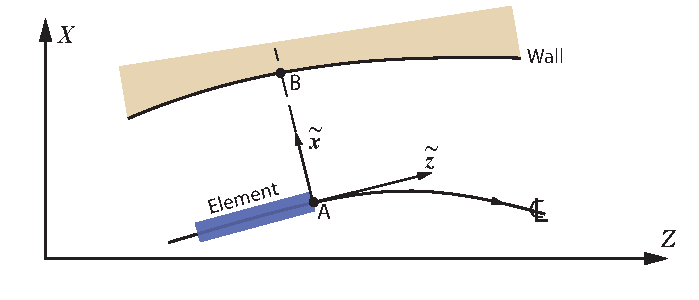
\includegraphics[width=5in]{building-wall-constraint.pdf}
  \caption[Building wall datum]
{A \vn{wall.} datum is a measure of the distance between the
centerline of a machine and the walls of the containment building.}
  \label{f:wall.constraint}
\end{figure}

  %----------------------
  \item[velocity, velocity.x, .y, .z] \Newline \hlabel{velocity}
The velocity normalized by the speed of light $c$.

  %----------------------
  \item[wall.left_side, .right_side] \Newline \hlabel{wall}
The \vn{wall} data data type is used to constrain the shape of a machine to fit inside a building's
walls (\sref{s:building.wall}). The general layout is shown in Figure~\ref{f:wall.constraint}. The
machine centerline is projected onto the horizontal $(Z, X)$ plane in the Global (floor) coordinate
system. Point \vn{A} is an evaluation point at the exit end of some element. $\wt z$ is the
projection of the local $z$-axis onto the $(Z, X)$ plane and $\wt x$ is the coordinate in the $(Z,
X)$ plane perpendicular to $\wt z$. In the typical situation, where a machine is planer (no
out-of-plane bends), the $\wt z$-axis corresponds to the local laboratory $z$-axis and the $\wt
x$-axis corresponds to the local laboratory $x$-axis (see the \bmad manual for an explanation of
local and global coordinate systems).

The distance from the machine at point \vn{A} to the wall is defined to be the distance from \vn{A}
to a point \vn{B} on the wall where point \vn{B} is along the $\wt x$ axis (has $\wt z = 0$) as
shown in Figure~\ref{f:wall.constraint}.

By definition, the \vn{``left side''} of the machine corresponds to be the $+\wt x$ side and the
\vn{``right side''} corresponds to be the $-\wt x$ side. That is, left and right are relative to
someone looking in the same direction as the beam is propagating. Correspondingly, there are two
wall data types: \vn{wall.left_side} and \vn{wall.right_side}. With the \vn{wall.left_side} data
type, the datum value is positive if point \vn{B} is on the left side and negative if on the
right. Vice versa for a \vn{wall.right_side} datum.  That is, there is interference with with wall
when the datum value is negative. If there are multiple wall points \vn{B}, that is, if there are
multiple points on the wall with $\wt z = 0$, the datum value will be the minimum value. Notice that
only wall sections that have a \vn{constraint} matching the datum will be used when searching for
possible points \vn{B}. If there are no wall points with $\wt z = 0$, the datum will be marked
invalid.

For \vn{wall} data there can be no reference element since this does not make sense.

Note: To constrain the machine vertically, use the \vn{floor.y} datum type. To constrain the length of
the machine, use the \vn{s_position} datum type.

  %----------------------
  \item[wire.<angle>] \Newline \hlabel{wire}
\vn{wire} data simulates the measurement of a wire scanner. The angle
specified is the angle of the wire with respect to the horizontal
axis. The measurement then measures the second moment $<uu>$ along an
axis which is 90 degrees off of the wire axis. For example,
\vn{wire.90} is a wire scanner oriented in the vertical direction and
measures the second moment of the beam along the horizontal axis,
$<xx>$. The resultant data is not the beam size, but the beam size
squared.

  \end{description}


\chapter{Plotting}
\index{plotting}
\label{c:plotting}

\begin{figure}[b]
  \centering
  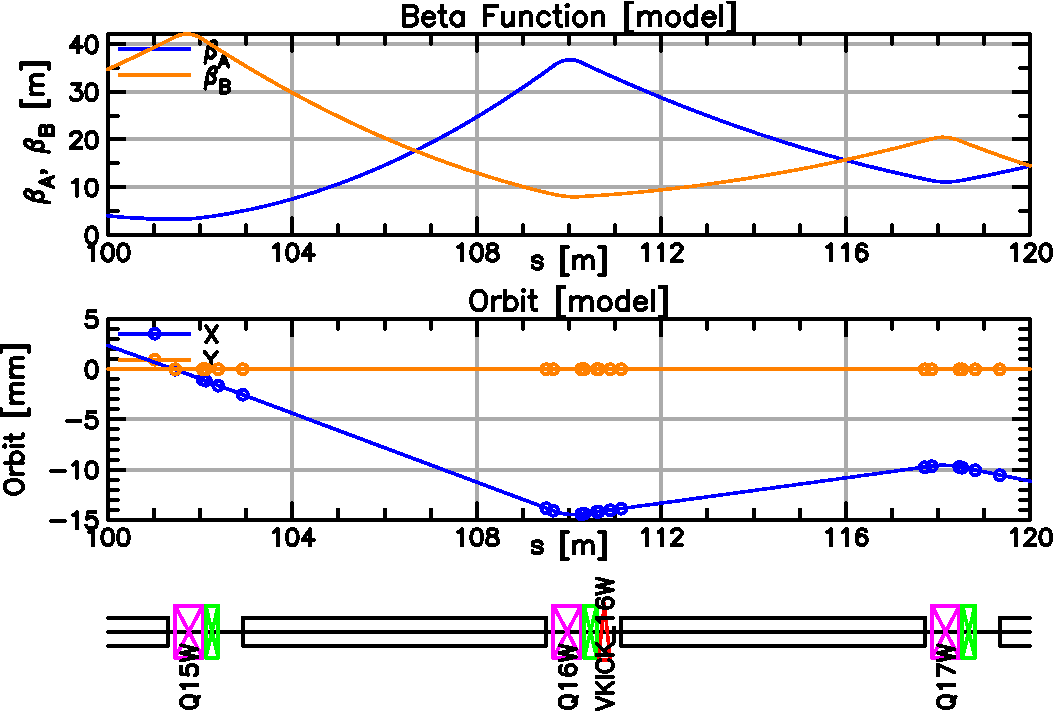
\includegraphics[width=4.5in]{plot-typical.pdf}
  \caption[An example of a plot display.]
{An example of a plot display. In this example there are three graphs: A graph displaying the beta
function, a graph displaying the orbit, and a graph displaying the ``lattice layout'' which shows
the longitudinal positions of lattice elements.}
  \label{f:plot.typ}
\end{figure}

\tao has a graphical display window within which such things as lattice functions, machine layout,
beam positions, etc., can be plotted. An example is shown in \fig{f:plot.typ} where there are plots
of the beta function and orbit along with a ``lattice layout which shows the longitudinal positions
of lattice elements. 

\tao organizes the display window using a number of concepts which are explained in the 
sections below
\begin{example}
  plot_page     ! The display window containing the graphics (\sref{s:plot.page.def}).
  regions       ! A set of rectangles on the plot_page that plots can be put in (\sref{s:region.def}).
  plot          ! A collection of graphs (\sref{s:plot.def}).
  box           ! Rectangular area within a plot that a graph is placed in (\sref{s:box.def}).
  graph         ! A diagram of some sort (\sref{s:graph.def}).
  curve         ! Data displayed within a \vn{graph} (\sref{s:curve.def}).
\end{example}

Underlying all this is the \vn{quick_plot} software toolkit (\sref{s:quick.plot}) which was developed
for \bmad and \tao for graphics plotting.

%-----------------------

\begin{figure}[bt]
  \centering
  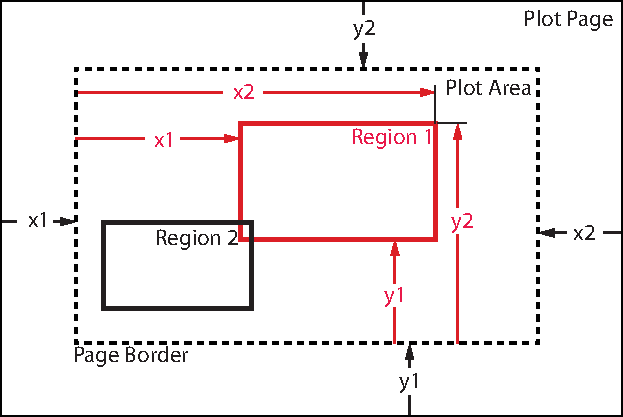
\includegraphics{plot-page.pdf}
  \caption[The plot window.]{The \vn{plot page} is the entire display window area. The \vn{plot area} 
is the region within the boarders of the \vn{plot page} within which ``\vn{regions}'' are
placed. The location of a \vn{region} is defined by four offsets with respect to the \vn{plot
area}. Regions may overlap.}
  \label{f:plot.page}
\end{figure}

%-----------------------------------------------------------------
\section{Plot Page}
\label{s:plot.page.def}

The \vn{plot page}, sometimes called the \vn{plot window}, refers to the window or the corresponding
printed graphics page where graphics are displayed. A \vn{plot page} is shown schematically in
\fig{f:plot.page}. Parameters associated with the \vn{plot page} are discussed in
\sref{s:plot.page}.  These parameters may be set in an initialization file or may be set on the \tao
command line using the \vn{set plot_page} (\sref{s:set.plot.page}) command. Examples:
\begin{example}
  set plot_page text_height = 11  ! 11 point font size
  set plot_page border%x1 = 0.2   ! Set left page border to 20% of width.
\end{example}

The size of the \vn{plot page} is set by the \vn{plot_page%size} parameter which is an array of two
numbers which set the width and height. The \vn{plot page} size can also be set when invoking \tao
using the \vn{-geometry} option (\sref{s:command.line})
\begin{example}
  > tao -lattice lat.bmad -geometry 300x500
\end{example}
This starts \tao with the \vn{plot page} size set to 300 points wide by 500 points high. It is also
sometimes convenient to start \tao without the plotting window. In this case, the \vn{-noplot} option
can be used on the startup command line. In a \tao initialization file, display of the plot window can be set
using the \vn{global%plot_on} parameter set in the \vn{tao_params} namelist (\sref{s:globals}).

In some cases, the screen resolution reported to \tao can be off. This has happened with some high
resolution displays where the reported resolution is 96 dpi when in fact the actual resolution is
much larger. In such a case, the size of the plot window created by \tao will be off. This can be
corrected by setting \vn{plot_page%size} appropriately but this in turn can create font size
problems. To avoid this problem, the environmental variable \vn{ACC_DPI_RESOLUTION} can be set to
the correct resolution before running \tao. The shell command line would be something like
\begin{example}
  > export ACC_DPI_RESOLUTION=168
\end{example}

The \vn{plot page} has a border within which \vn{regions} (\sref{s:region.def}) are defined. The area withing
the plot page border is called the \vn{plot area}

The \vn{show plot -page} (\sref{s:show.plot}) command may be used to view the page parameters.

%-----------------------------------------------------------------
\section{Region}
\label{s:region.def}

The \vn{plot area} is the area within the border of the \vn{plot page} as shown in
\fig{f:plot.page}.  In this \vn{plot area}, ``\vn{regions}'' can be defined which are invisible
rectangles where a \vn{plot} (\sref{s:plot.def}) can be placed. This is shown schematically in
\fig{f:plot.page}. Each region has a name and four numbers which specifies the location of the
region within the plot area. Regions may be defined by the user. In addition, for convenience, \tao
will define a number of regions. \tao defined regions will either begin with the letter ``\vn{r}''
or begin with the string ``\vn{layout}'' or the string ``\vn{scratch}''. Regions may overlap. How to
define regions is explained in \sref{s:plot.page}. The \vn{show plot} command will show the region
list. Example:
\begin{example}
  Tao> show plot

Plot Region         <-->  Plot                 x1    x2    y1    y2     Visible
-----------               -----------------------------------------------------
layout              <-->  lat_layout          0.00  1.00  0.00  0.15         T
r11                 <-->                      0.00  1.00  0.15  1.00
r12                 <-->                      0.00  1.00  0.58  1.00
r22                 <-->                      0.00  1.00  0.15  0.58
r13                 <-->  beta                0.00  1.00  0.72  1.00         T
r23                 <-->  dispersion          0.00  1.00  0.43  0.72         T
r33                 <-->  orbit               0.00  1.00  0.15  0.43         T
r14                 <-->                      0.00  1.00  0.79  1.00
\end{example}
The \vn{Plot} column shows what \vn{plot} (if any) is associated with the region
(\sref{s:plot.def}). The next four columns show the values of \vn{x1}, \vn{x2}, \vn{y1}, and \vn{y2}
set for the region. As shown in \Sref{s:plot.page}, \vn{x1} and \vn{x2} are the offsets from the
left \vn{plot area} edge to the left and right edges of the region. Similarly, \vn{y1} and \vn{y2}
are the offsets from the bottom edge of the \vn{plot area} to the bottom and top edges of the
region. \vn{x1} and \vn{x2} are normalized by the \vn{plot area} width and \vn{y1} and \vn{y2} are
normalized by the \vn{plot area} height so all four numbers should be in the range $[0, 1]$.  Using
the above example, the \vn{r23} region spans the full width of the \vn{plot area} (since \vn{x1} = 0
and \vn{x2} = 1), and occupies approximately the middle third vertically of the \vn{plot area}
(since \vn{y1} = 0.43 and \vn{y2} = 0.72).

The last column in the above shows if the \vn{plot} associated with the \vn{region} is
visible. Normally everything is visible. Invisibility is used in some special cases. For example,
when using a Graphical User Interface (GUI).

The \vn{set region} command can be used to set region parameters. Example:
\begin{example}
  set region r13 y1 = 0.8  ! Sets lower edge vertical position
\end{example}

%-----------------------------------------------------------------
\section{Plot}
\label{s:plot.def}

A \vn{plot} is essentially a collection of \vn{graphs}. This is shown schematically in
\fig{f:plot.plot} which shows a plot with two graph side by side.

Plots are divided into two groups. A \vn{template} plot defines how a \vn{displayed} plot is to be
constructed. That is, a \vn{template} plot defines what the associated \vn{graphs} are, defines
graph placement within the plot, etc. When a \vn{template} plot is \vn{placed} in a \vn{region},
either by using the \vn{place} command (\sref{s:place}) or by placement defined in an initialization
file (\sref{s:plot.page}), the information of the \vn{template} is copied in order to construct a
\vn{displayed} plot. A given \vn{template} plot may be placed in multiple \vn{regions} to give
multiple \vn{displayed} plots and then, using \vn{set} commands, the data displayed in each of these
plots may be manipulated separately. For example, one displayed orbit plot could show the orbit of
the \vn{model} lattice while another orbit plot could show the orbit difference between the
\vn{model} and \vn{design} lattices. When a \vn{plot} is displayed in a given \vn{region},
everything drawn is scaled to the region size.

Use the \vn{show plot} to see what displayed plots are associated with what regions. Use the
\vn{show plot -templates} command to see a list of \vn{template} plots. \tao defines a number of
default \vn{template} plots. Section~\sref{s:template} discusses how to define custom template
plots in an initialization file. Use the \vn{set plot} command (\sref{s:set.plot}) to modify either
\vn{template} or \vn{displayed} plots.

All plots have a name. A \vn{displayed} plot will inherit the same name of the \vn{template} plot it
came from. If a given \vn{template} plot is used to create multiple \vn{displayed} plots. All of
these plots will have the same name. A \vn{displayed} plot can also be referred to by using the
associated \vn{region} name. This can be used to remove ambiguity if there are multiple
\vn{displayed} plots of the same name. Additionally, a \vn{template} plot can unambiguously be
referred to by adding the prefix ``\vn{T::}'' to the plot name. Examples:
\begin{example}
  show plot           ! Show plots associated with regions
  show plot -template ! Show template plots
  place r13 orbit     ! Put orbit template into r13 region
\end{example}

Some commands, for example, the \vn{scale} command by default will ignore \vn{template} plots unless
the plot name has the \vn{T::} prefix. Other commands, for example the \vn{show plot} command, will
preferentially show displayed plot info but will show template plot info if there are no matching
displayed plots. Examples:
\begin{example}
  scale orbit -10 10    ! Scale all displayed orbit plots. Ignore template.
  scale r33 -10 10      ! Scale only plot in r33 region.
  scale T::orbit -10 10 ! Scale template orbit plot.
  show plot e_field     ! Will show displayed e_field plot info. If no
                        ! displayed plot exists, will show template info.
\end{example}

%-----------------------

\begin{figure}[bt]
  \centering
  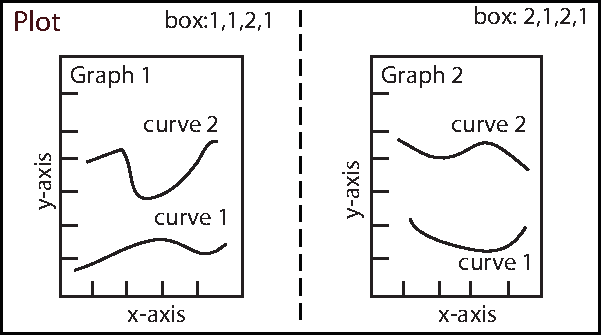
\includegraphics[width=5.0in]{plot-plot.pdf}
  \caption[Plotting nomenclature.]
  {
A plot has a collection of graphs and a graph has a collection of curves. A graph is located within
a plot by defining the ``\vn{box}'' associated with the \vn{graph}. Illustrated here is a plot with
two graphs placed side by side.
  }
  \label{f:plot.plot}
\end{figure}

%-----------------------------------------------------------------
\section{Box}
\label{s:box.def}

To determine where a \vn{graph} is drawn with respect to the boundaries of its associated \vn{plot},
each \vn{graph} is associated with a given ``\vn{box}''. A \vn{box} is a rectangular sub-region of
the \vn{plot}. Boxes are defined by dividing the \vn{plot} into a rectangular grid and then choosing
one of the grid rectangles to be the \vn{box} associated with the \vn{graph}. The is illustrated in
\fig{f:plot.plot} where \vn{Graph 1} is associated with the \vn{box} labeled ``\vn{1,1,2,1}'' and
\vn{Graph 2} is associated with the \vn{box} labeled \vn{2,1,2,1}.  The last two digits of a
\vn{box} label (\vn{2,1} for both graphs) specify the number of rectangles the grid has horizontally
and vertically (2 horizontally, 1 vertically here). The first two digits (\vn{1,1} for \vn{graph 1}
and \vn{2,1} for \vn{graph 2}) specify the particular rectangle associated with the \vn{box} with
\vn{1,1} designating the lower left rectangle. Different \vn{graphs} do not have to use the same
grid division to select a box from.

Setting the \vn{box} for a given \vn{graph} in a \tao initialization file is covered in \sref{s:template}.
The \vn{set graph} and \vn{show graph} commands can be used to set and show the box parameters. 
Examples:
\begin{example}
  set graph myplot.g1 box = 2 1 2 2  ! Set box of graph myplot.g1
  set graph myplot.g2 box = 1 1 1 2  ! Different graphs can use different grids
                                     !  for box selection
\end{example}

%-----------------------------------------------------------------
\section{Graph}
\label{s:graph.def}

%-----------------------------------------------------------------
\subsection{Overview}
\label{s:graph.overview}

A \vn{graph} is a diagram of some sort. Most \vn{graph}s consists of horizontal and vertical axes
along with one or more \vn{curve}s. \vn{Floor_plan} (\sref{s:floor.plan}) and \vn{lat_layout}
(\sref{s:lat.layout}) \vn{graphs}, on the other hand, shows the placement in space of the lattice
elements and do not have any associated \vn{curves}.

Every \vn{plot} has at least one \vn{graph}. How many \vn{graphs} are associated with a \vn{plot}
is a matter of convenience and different \vn{graphs} of a \vn{plot} may display different types of
information. For example, it would be possible to have a single \vn{plot} contain three \vn{graphs}
and look like what is shown in \fig{f:plot.typ}. In actuality, the figure was constructed using
three \vn{plots} each one containing one \vn{graph}.

How to define \vn{graphs} when defining \vn{template} plots is given in \sref{s:template}. The
\vn{show graph} command can be used to show graph parameters. The \vn{set graph} command can
be used to modify \vn{graph} parameters.

%-----------------------------------------------------------------
\subsection{Graph Name}
\label{s:graph.name}

All graphs have a name. For example, the graph of the standard \vn{orbit} plot is simply ``\vn{g}''.
\vn{Graphs} may be referred to using the syntax:
\begin{example}
  <plot>.<graph>
\end{example}
where \vn{<plot>} is the plot name (or the \vn{region} name associated with the \vn{plot}) and
\vn{<graph>} is the graph name. If the \vn{.<graph>} ending is omitted, all graphs of the named
\vn{plot}(s) are selected. Examples:
\begin{example}
  show graph beta   ! Show info of all graphs in all the displayed beta plots.
  show graph r13.g1 ! Show info on ``g1'' graph of region r13.
\end{example}

%-----------------------------------------------------------------
\subsection{Curve Legend of a Graph}
\label{s:curve.legend}

The \vn{curve legend} is the legend identifying what curves are associated with what perimeters. In
\fig{f:plot.typ} the top two graphs have a curve legend in the upper left hand corner of the graph.
By default, the \vn{data_type} of each curve will be used as the text for that
curve's line in the legend.  This default can be changed by setting a curve's \vn{curve%legend_tex}.
Parameters that affect the curve legend are:
\begin{example}
  plot_page%legend_text_scale        ! Also affects lat_layout and floor_plan text size.      
  curve(N)%legend_text               ! 
  graph%curve_legend_origin          
  graph%draw_curve_legend            
  graph%curve_legend%line_len    ! curve_legend is a qp_legend_struct (\sref{s:qp.legend.str}).
  graph%curve_legend%text_offset ! 
\end{example}
The curve legend is distinct from the \vn{text legend} (\sref{s:text.legend}).

%-----------------------------------------------------------------
\subsection{Text Legend}
\label{s:text.legend}

The \vn{text legend} is a legend that can be setup by either the user or by \tao itself.
\tao uses the text legend in conjunction with phase space plotting or histogram displays.
The \vn{text legend} is distinct from the \vn{curve legend}. Parameters that affect the text
legend are:
\begin{example}
  graph%text_legend(:)      ! Array of strings to print
  graph%text_legend_origin  ! Position of legend.
\end{example}

%-----------------------------------------------------------------
\subsection{Graph Types}
\label{s:graph.types}

\tao defines several kinds of graphs. The \vn{graph%type} in the \vn{tao_template_graph}
(\sref{s:template}) sets the type.
\begin{description}
%
\item["data"] \Newline
``Data'' plotting is the plotting of a dependent variable on the $y$-axis vs an independent variable
on the $x$-axis. Typically the independent variable will be the longitudinal position $s$-position
as in the upper two graphs in \fig{f:plot.typ}. Also see \Sref{s:draw.ap} for an example where beam
apertures are added to the graph.

A ``\vn{data slice}'' graph is plotting one data array on the $y$-axis versus another data array on
the $x$-axis (\sref{s:graph.data.slice}). Also see \vn{parametric plotting} (\sref{s:param.plot}).

With a \vn{parametric} plot both the $x$ and $y$ values of the points on a curve are dependent
upon an independent parameter (\sref{s:param.plot}). This is similar to a \vn{data slice} plot
(\sref{s:graph.data.slice}).
%
\item["dynamic_aperture"] \Newline
A \vn{dynamic aperture} graph (\sref{s:da.plot}) draws the results from a dynamic aperture
calculation (\sref{s:da.calc}).
%
\item["floor_plan"] \Newline
A \vn{floor plan} graph shows the physical layout of the machine (\sref{s:floor.plan}). A table maps
lattice elements to a shape that is drawn (\sref{s:shapes}). The user may override the default
mapping. Besides the lattice elements. the outline of the building or tunnel that the machine is in
can be drawn (\sref{s:building.wall}).
%
\item["histogram"] \Newline
Currently \vn{histograms} (\sref{s:histogram}) are limited to displaying phase space data.
%
\item["key_table"] \Newline
The \vn{key table} displays information about variables bound to keyboard keys \sref{s:key.bind}.
Key bindings are used in \vn{single mode}.
%
\item["lat_layout"] \Newline
A \vn{lattice layout} graph displays the lattice elements as a series of shapes as a function of the
longitudinal position $s$ (\sref{s:lat.layout}). The lowest graph in \fig{f:plot.typ} is an example
of a \vn{lattice layout}.  A table maps lattice elements to a shape that is drawn (\sref{s:shapes}).
The user may override the default mapping.
%
\item["phase_space"] \Newline
A \vn{phase space graph} (\sref{s:phase.space}) displays particle positions in phase space after
a beam of particles has been tracked (\sref{s:beam.init}).
%
\item["wave.0", "wave.a", "wave.b"] \Newline
Wave analysis plotting (\sref{c:wave}).
%
\end{description}

\begin{figure}[b]
  \centering
  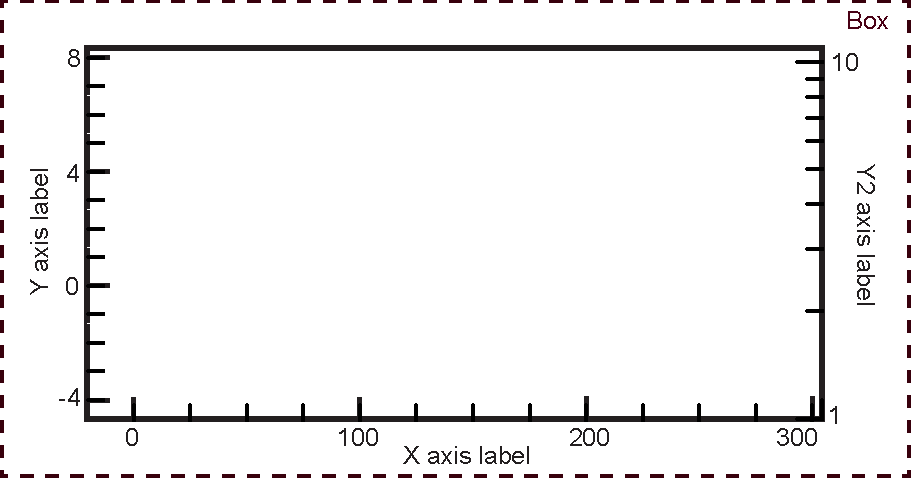
\includegraphics[width=5.0in]{plot-axes.pdf}
  \caption[Plot axes.]
{A data graph has three axes called \vn{x} (bottom edge), \vn{y} (left edge), and \vn{y2} (right edge).}
  \label{f:plot.axes}
\end{figure}

%-----------------------------------------------------------------
\subsection{Graph Axes}
\label{s:axes}

Data graphs (\sref{s:graph.types}) have three axes as shown in \fig{f:plot.axes}. The bottom axis is
called \vn{x}, and the left and right axes are called \vn{y} and \vn{y2} respectively. The
\vn{qp_axis_struct} structure (\sref{s:qp.axis}) is used to store axis parameters which can be
accessed via the \vn{graph%x}, \vn{graph%y}, and \vn{graph%y2} components in the
\vn{tao_template_graph} namelist (\sref{s:template}) or by using the \vn{set graph} command
(\sref{s:set.graph}.

The \vn{scale} command (\sref{s:scale}) can be used to set the vertical axes. The \vn{x_scale}
(\sref{s:x.scale}) command can be used to set the horizontal axis.

Normally there is only one vertical scale for a graph and this is associated with the \vn{y}
axis. However, if any curve of a given graph has \vn{curve%use_y2} set to \vn{True} then the \vn{y2}
axis will have an independent second scale. In this case, the \vn{y2} axis numbers will be
drawn. Notice that simply giving the \vn{y2} axis a label does {\em not} make the \vn{y2} axis scale
independent of the \vn{y} axis scale.

The following \vn{tao_plot_page} namelist (\sref{s:plot.page}) parameters affect the drawing of the axes:
\begin{example}
  text_height = 12              ! In points. Scales the height of all text
  axis_number_text_scale = 0.9  ! Relative to text_height
  axis_label_text_scale = 1.0   ! Relative to text_height
\end{example}

%-----------------------------------------------------------------
\section{Curve}
\label{s:curve.def}

%-----------------------------------------------------------------
\subsection{Overview}
\label{s:curve.overview}

A \vn{curve} is a data set to be displayed within a \vn{graph}. For example, a \vn{curve} may be the
beta function of the \vn{model} lattice. \vn{Curves} have an associated set of points at which a
symbol can be drawn. A curve also can have an associated curved line that can be drawn. For example,
in \fig{f:plot.typ} only the line is drawn with the two curves of the beta plot while both symbols
and line are drawn for the two curves of the orbit plot (here the data points where symbols are
drawn are the orbit at the edges of the lattice elements).

Some \vn{graphs} do not have any associated curves. For example, a \vn{lat_layout} graph does not
have associated curves.

How to define \vn{curves} when defining \vn{template} plots is given in \sref{s:template}. The
\vn{show curve} command can be used to show curve parameters. The \vn{set curve} command can
be used to modify \vn{curve} parameters.

%-----------------------------------------------------------------
\subsection{Curve Name}
\label{s:curve.name}

All curves have a name. \vn{Curves} may be referred to using the syntax:
\begin{example}
  <plot>.<graph>.<curve>
\end{example}
where \vn{<plot>} is the plot (or \vn{region}) name, \vn{<graph>} is the graph name and \vn{<curve>}
is the curve name. If the \vn{.<curve>} ending is omitted, all curves of the named \vn{graph}(s) are
selected. If the \vn{.<graph>.<curve>} ending is omitted, all curves of the named \vn{plot}(s) are
selected. Examples:
\begin{example}
  show curve beta   ! Show info of all curves in all the displayed beta plots.
  show curve r13.g1 ! Show info on curves in ``g1'' graph of region r13.
  set graph orbit.g curve_legend_origin = 0.1 -0.2 "%BOX/LT"  ! Set curve legend origin
\end{example}
The last example sets the \vn{curve legend} (\sref{s:template}) of the graph so that the curve
legend of the graph is drawn with respect to the left top corner of the box.

%-----------------------------------------------------------------
\subsection{Curve Line}
\label{s:curve.line}

Each curve may have an associated line that is drawn. The line may be a set of line segments
connecting curve symbol points (\sref{s:curve.sym}) or may be a ``smooth'' curve calculated by
evaluating the curve at a number of points. 

\vn{curve%draw_line} determines whether a curve is drawn through the data point symbols. The
thickness, style (solid, dashed, etc.), and color of the line can be controlled by setting
\vn{curve%line}. If \vn{plot%x_axis_type} is \vn{"s"}, and \vn{curve%component} does not contain
\vn{"meas"} or \vn{"ref"}, \tao will attempt to calculate intermediate values in order to draw a
smooth, accurate curve is drawn. Occasionally, this process is too slow or not desired for other
reasons so setting \vn{curve%smooth_line_calc} to False will prevent this calculation and the curve
will be drawn as a series of lines connecting the symbol points. The default of
\vn{curve%smooth_line_calc} is True. Use the \vn{set curve} command (\sref{s:set}) to toggle the
drawing of lines. Alternatively, the \vn{-disable_smooth_line_calc} switch can be used on the
command line (\sref{s:command.line}) or the global variable \vn{global%disable_smooth_line_calc} can
be set in the \tao initialization file (\sref{s:globals}).

The number of points to evaluate at when constructing a smoothed line is set by
\vn{plot_page%n_curve_pts} in the \vn{tao_plot_page} namelist (\sref{s:plot.page}) or by using the
\vn{set plot_page} command (\sref{s:set.plot.page}). To override this value for a particular plot
the \vn{plot%n_curve_pts} parameter can be set in the \vn{tao_template_plot} namelist or using the
\vn{set plot} command (\sref{s:set.plot}). More evaluation points may give a more accurate curve at
the expense of computation time.

%-----------------------------------------------------------------
\subsection{Curve Symbol}
\label{s:curve.sym}

\vn{curve%draw_symbols} determines whether a symbol is drawn at the data points. The size, shape and
color of the symbols is determined by \vn{curve%symbol}. A given symbol point that is drawn has
three numbers attached to it: The $(x, y)$ position on the graph and an index number to help
identify it. The index number of a particular symbol is the index of the datum or variable
corresponding the symbol in the \vn{d1_data} or \vn{v1_var} array. These three numbers can be
printed using the \vn{show curve -symbol} command (\sref{s:show}).  \vn{curve%draw_symbol_index}
determines whether the index number is printed besides the symbol. Use the \vn{set curve} command
(\sref{s:set}) to toggle the drawing of symbols. The default value for \vn{curve%draw_symbol} is
False if \vn{plot%x_axis_type} is \vn{"s"}, \vn{"curve"}, \vn{"lat"}, or \vn{"var"} and True
otherwise. The default \vn{curve%draw_symbol_index} is always False.

The \vn{graph%draw_only_good_user_data_or_vars} logical determines whether datums
(\sref{s:init.data}) or variables (\sref{s:init.var}) with a \vn{good_user} component set to
\vn{False} are drawn. The default is to not draw them which means that data or variables not used in
an optimization are not drawn.

%-----------------------------------------------------------------
\subsection{Curve Component}
\label{s:curve.comp}

A ``\vn{data}'' graph (\sref{s:graph.types}) is used to draw lattice parameters such as orbits, or
\tao data (\sref{c:data}), or variable values such as quadrupole strengths. The data values will
depend upon where the data comes from. This is determined, in part, by the setting of the
\vn{component} parameter in the \vn{tao_template_graph} namelist (\sref{s:template}).  The
\vn{component} may be one of:
\index{model}\index{design}\index{base}\index{meas}\index{ref}
\begin{example}
  "model"             ! model values. Default.
  "design"            ! design values.
  "base"              ! Base values
  "meas"              ! data values.
  "ref"               ! reference data values.
  "beam_chamber_wall" ! Beam chamber wall
\end{example}
Additionally, \vn{component} may be set to plot a linear combination of the above. For
example:
\begin{example}
  &tao_template_graph
    curve(2)%component = "model - design"
    ...
\end{example}
This will plot the difference between the \vn{model} and \vn{design} values. 
The default value of \vn{%component} is \vn{"model"}.

%-----------------------------------------------------------------
\subsection{Curve Data Source}
\label{s:curve.source}

\index{data}\index{var}\index{calculation}
\index{curve!data_source}
The \vn{data_source} parameter of a curve is the type of information for the source of the data points.
\vn{data_source} must be one of:
\begin{example}
  "data"              ! A d1_data array is the source of the curve points.
  "var"               ! A v1_var array is the source of the curve points.
  "lat" (Default)     ! The curve points are computed directly from the lattice.
  "beam"              ! The curve points are computed from tracking a beam of particles.
  "multi_turn_orbit"  ! Computation is from multi-turn tracking. 
\end{example}
The default for \vn{data_source} is \vn{"lat"}. With \vn{data_source} set to "\vn{data}",
the values of the curve points come from the \vn{d1_data} array structure named by
the curve's \vn{data_type} parameter (\sref{s:curve.type}).

If \vn{data_source} is set to \vn{var}, the values of the curve points come from a \vn{v1_var}
array structure. If it is set to \vn{lat} the curve data points are calculated from the lattice
without regard to any data structures. \vn{data_source} can be set to \vn{beam} when tracking
beams of particles. In this case, the curve points are calculated from the tracking. With \vn{beam},
the particular bunch that the data is extracted from can be specified via \vn{ix_bunch}. The
default is \vn{0} which combines all the bunches of the beam for the calculation.

Used in conjunction with \vn{data_type} and \vn{component} (\sref{s:curve.comp}). For
example (\sref{s:curve.source}), a curve of the orbit with \vn{data_source} set to \vn{"beam"}
would use the beam centroid computations. If the \vn{data_source} was set to \vn{"lat"} the
computed orbit using single particle tracking is used.

Example: With \vn{data_type} set to \vn{beta.x}, the setting of \vn{data_source} to
\vn{lat} gives the beta as calculated from the lattice and \vn{beam} gives the beta as calculated
from the shape of the beam.

%-----------------------------------------------------------------
\subsection{Curve Data Type}
\label{s:curve.type}

The \vn{data_type} of a curve specifies what is being plotted. What the valid settings for \vn{data_type}
are depends upon the type of graph (\sref{s:graph.types}). 
\begin{description}
%
\item[graph\%type = "data", or "histogram"] \Newline
Valid settings for \vn{data_type} are any \tao datum type (\sref{s:data.table}), \tao variable
(\sref{c:var}), and the following electric and magnetic field components:
\begin{example}
  b0_field.x,  b0_field.y,  b0_field.z,  b0_curl.x,  b0_curl.y,  b0_curl.z,  b0_div
  e0_field.x,  e0_field.y,  e0_field.z,  e0_curl.x,  e0_curl.y,  e0_curl.z,  e0_div
\end{example}
The field data types with names starting with ``b_'' and ``e_'' evaluate the field along the single
particle trajectory while the field data types with names starting with ``b0_'' and ``e0_'' are evaluated
along a constant transverse position specified by the curve's \vn{orbit} parameter.
%
\item[graph\%type = "dynamic_aperture"] \Newline
Valid settings for \vn{data_type} are:
\begin{example}
  "beam_ellipse"
  "dynamic_aperture"
\end{example}
%
\item[graph\%type = floor_plan", "lat_layout", or "key_table"] \Newline
There are not curves associated with these graph types.
%
\item[graph\%type = "phase_space"] \Newline
Valid settings for \vn{data_type} are:
\begin{example}
  "x",  "px",  "y",  "py",  "z",  "pz",
  "intensity",  "intensity_x",  "intensity_y"     ! Photon intensity
  "phase_x", "phase_y"                            ! Photon coherent phase
\end{example}
%
\end{description}

 For example, with \vn{graph%type} set to
\vn{dynamic_aperture} the 




Thus in the above example the curve point values are obtained from
\vn{orbit.x} data. To be valid the data structure named by \vn{data_type} must be set up in an
initialization file. If not given, the default \vn{data_type} is
\begin{example}
  <plot%name>.<graph%name>
\end{example}

%-----------------------------------------------------------------
\section{Quick_Plot Plotting}
\label{s:quick.plot}

\vn{Quick_plot} is a software library developed for \bmad and \tao for graphics plotting.

%-----------------------------------------------------------------
\subsection{Length and Position Units}
\label{s:qp.units}

Positions and lengths with \vn{quick_plot} generally have an associated ``\vn{units}'' string which determines how
$(x, y)$ positions or $(dx, dy)$ lengths are to be interpreted. 
The syntax of the \vn{units} parameter is:
\begin{example}
  "unit_type/ref_object/corner"
\end{example}
A \vn{units} string has a \vn{unit_type}, \vn{ref_object} and \vn{corner} components separated by slashes ``/''.

The \vn{unit_type} component is the type of units which can be one of:
\begin{example}
   "%"       - Percent.
   "DATA"    - Data units associated with a graph.
   "MM"      - millimeters.
   "INCH"    - Inches.
   "POINTS"  - Printers points (72 points = 1 inch, 1 pt ~ 1 pixel).
\end{example}
Note: If \vn{unit_type} is set to \vn{"DATA"}, \vn{ref_object}, if present, must be \vn{"GRAPH"} and
\vn{corner}, if present, must be \vn{"LB"}.

The \vn{ref_object} component is a reference object which can be one of:
\begin{example}
   "PAGE"  -- Relative to the plot display window.
   "BOX"   -- Relative to the box the graph is associated with.
   "GRAPH" -- Relative to the graph rectangle.
\end{example}
The \vn{ref_object} component is optional if a relative length is being specified and the
\vn{unit_type} is anything other than \vn, the slash between
the \vn{unit_type} and the \vn{ref_object} may be omitted.

Note: The \vn{"PAGE"} reference is the entire \vn{plot page} and not the \vn{plot area}. The
\vn{plot area} is only used for defining the placement of \vn{regions}.

The \vn{corner} component is the origin location of the reference object.
\vn{corner} can be one of:
\begin{example}
   "LB" -- Left Bottom of reference object. Default.
   "LT" -- Left Top.
   "RB" -- Right Bottom.
   "RT" -- Right Top.
\end{example}
The \vn{ref_object} component is optional if a relative length is being specified.

Examples:
\begin{example}
  "DATA"          -- Equivalent to "DATA/GRAPH/LB"
  "DATA/GRAPH/LB" -- Same as above.
  "DATA/BOX/RT"   -- ILLEGAL: DATA must always go with GRAPH/LB.
  "%/PAGE/LT"     -- Equivalent to "%PAGE/LT"
  "%PAGE/LT"      -- Percentage of page so (0.0, 1.0) = RT of page.
  "%BOX"          -- Percentage of box so (1.0, 1.0) = RT of box.
  "INCH/PAGE"     -- Inches from LB of page. Equivalent to "INCH/PAGE/LB"
\end{example}

Units can be set in an initialization file or with the \vn{set} command. Example:
\begin{example}
  set plot_page title%units = '%PAGE'
\end{example}

%-----------------------------------------------------------------
\subsection{Text Justification Units}
\label{s:qp.str.just}

Text justification units is a two character string that sets where a line of text is to be printed
with respect to the text $(x, y)$ position.
The first character of the justification string gives the horizontal alignment:
\begin{example}
   "L" -- Left justify
   "C" -- Center justify
   "R" -- Right justify
\end{example}
The second character of the justification string gives the vertical alignment:
\begin{example}
   "B" -- Bottom justify
   "C" -- Center justify
   "T" -- Top justify
\end{example}

Example:
\begin{example}
  plot_page%title%justify = 'CC'
\end{example}

%-----------------------------------------------------------------
\subsection{qp_point_struct}
\label{s:qp.point}

\vn{QuickPlot} defines a number of structures to parameterize such things like line and symbol
properties.

The \vn{qp_point_struct} defines where a point is:
\begin{example}
  type qp_point_struct:
    x     = <real>     ! Horizontal offset of point from fiducial point
    y     = <real>     ! Vertical offset of point from fiducial point
    units = "<units>"  ! Units of x \& y (\sref{s:qp.units}).
\end{example}
Example:
\begin{example}
  graph%curve_legend_origin = 5.0, -2.0, "POINTS/GRAPH/LT"
\end{example}
In this example the fiducial point the left-top point on the graph rectangle. The
\vn{curve_legend_origin} is positioned 5.0 points horizontally to the left and 2.0 points vertically
downward from this fiducial point.

%-----------------------------------------------------------------
\subsection{qp_line_struct}
\label{s:qp.line}

The parameters associated with data lines drawn in a graph are contained in the \vn{qp_line_struct}:
\begin{example}
  type qp_line_struct:
    width    = <integer>  ! Default = 1
    color    = <string>   ! Default = "black" (\sref{s:qp.color}).
    pattern  = <string>   ! Default = "solid" (\sref{s:qp.line.pat}).
\end{example}

%-----------------------------------------------------------------
\subsection{Symbols}
\label{s:qp.sym}

The parameters associated with symbols that are drawn are contained in the \vn{qp_symbol_struct}:
\begin{example}
  type qp_symbol_struct:
    type          = <string>  ! Default = "dot"
    height        = <real>    ! Size in points. Default = 10
    color         = <string>  ! Default = "black" (\sref{s:qp.color})
    fill_pattern  = <string>  ! Default = "solid_fill"
    line_width    = <integer> ! Default = 1.
\end{example}

\begin{table}
  \centering
  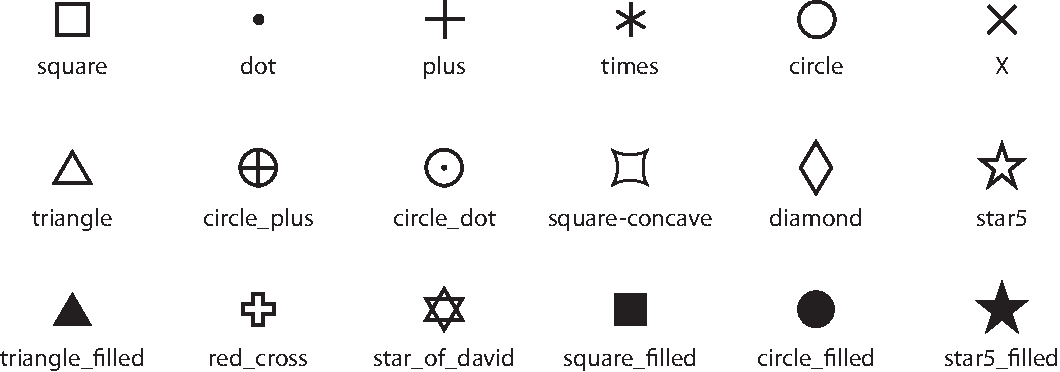
\includegraphics[width=5in]{plot-syms.pdf}
  \caption{Plotting Symbols.}
  \label{t:plot.syms}
\end{table}

The symbol types are:
\begin{example}
  square                 triangle                    square_concave              
  dot                    circle_plus                 diamond                     
  plus                   circle_dot                  star5                       
  times                  square_filled               triangle_filled           
  circle                 circle_filled               red_cross                 
  x                      star5_filled                star_of_david             
\end{example}
These symbols are illustrated in Table~\ref{t:plot.syms}. Symbol type names are case insensitive.

%-----------------------------------------------------------------
\subsection{qp_axis_struct}
\label{s:qp.axis}

The \vn{qp_axis_struct} structure defines the properties of a graph axis
\begin{example}
  type qp_axis_struct::
    label             = "<string>" ! Axis label string.
    min               = <real>     ! Min is the left or bottom axis number.
    max               = <real>     ! Max is the right or top axis number.
    number_offset     = <real>     ! Offset from axis line in inches.
    label_offset      = <real>     ! Offset from numbers in inches.
    major_tick_len    = <real>     ! Major tick length in inches.
    minor_tick_len    = <real>     ! Minor tick length in inches.
    label_color       = <string>   ! Color of the label string (\sref{s:qp.color})
    major_div         = <integer>  ! Number of major divisions
    major_div_nominal = <integer>  ! Major divisions nominal value.
    minor_div         = <integer>  ! Minor divisions. 0 = Tao will choose.
    minor_div_max     = <integer>  ! Max minor div number if Tao chooses.
    places            = <integer>  ! Number of digits to print
    type              = <string>   ! Axis type: "LINEAR" or "LOG".
    bounds            = <string>   ! Axis bounds: "GENERAL", "ZERO_AT_END", etc.
    tick_side         = <integer>  ! 1 = draw to the inside, 0 = both, -1 = outside.
    number_side       = <integer>  ! 1 = draw to the inside, -1 = outside.
    draw_label        = <logical>  ! Draw the label string
    draw_numbers      = <logical>  ! Draw the numbers.
\end{example}

The \vn{%bounds} parameter sets how the axes min and max values are calculated when plots are initially
instantiated and when \vn{scale}, \vn{x_scale}, and \vn{xy_scale} commands are used. Possible settings
are:
\begin{example}
  "ZERO_AT_END"      ! Min or max value is set to zero.
  "ZERO_SYMMETRIC"   ! Min and max chosen so that max = -min.
  "GENERAL"          ! No restrictions (default).
  "EXACT"            ! The User min/max is used.
\end{example}
If input min and max values are specified by the User, \tao will take the specified values as the starting
point to find ``nice'' min and max values to use. For example, with the command
\begin{example}
  scale all 0 19
\end{example}
and with \vn{bounds} set to \vn{"GENERAL"}, the min and max values will be set to 0 and 20. The exception is when
\vn{bounds} is set to \vn{"EXACT"}. In this case the User supplied min and max values will be used as is.

Examples:
\begin{example}
Tao> set graph r13 y%bounds = "zero_at_end"
Tao> scale r13 200 280   ! Graph bounds set to [0, 300]

Tao> set graph r13 y%bounds = "zero_symmetric"
Tao> scale r13 200 280   ! Graph bounds set to [-300, 300]

Tao> set graph r13 y%bounds = "general"
Tao> scale r13 20 190    ! Graph bounds set to [0, 200]

Tao> set graph r13 y2%bounds = "exact"
Tao> scale r13 -y2 20 190    ! Y2 graph bounds set to [20, 190]
\end{example}

Both \vn{major_div} and \vn{major_div_nominal} set the number of major divisions in the plot. The
difference between the two is that with \vn{major_div} set positive and \vn{major_div_nominal} set
zero or negative, the number of major divisions is fixed at the value of \vn{major_div}. With
\vn{major_div_nominal} positive, the value of \vn{major_div} is ignored, and the number of major
divisions will be chosen to be a ``nice'' value near the value of \vn{major_div_nominal}. If neither
\vn{major_div} nor \vn{major_div_nominal} is set positive, a value will be chosen for
\vn{major_div_nominal} by \tao. If you are unsure which to set, it is recommended that
\vn{major_div_nominal} be used.

The \vn{places} parameter set the number of places to display a number. \tao will automatically
calculate this number and it is not user settable.

The \vn{label} parameter may include Greek letters, subscripts, superscripts, and special characters.
Encoding for these are given in Table~\ref{t:plot.escape}. 

%-----------------------------------------------------------------
\subsection{qp_legend_struct}
\label{s:qp.legend.str}

The parameters associated with drawing a curve legend (\sref{s:plot.def}) are contained in the parameter
\vn{plot_page%curve_legend} (\sref{s:plot.page}). This parameter is an instance of a \vn{qp_legend_struct}
which has the structure:
\begin{example}
  type qp_legend_struct
    row_spacing = <real>           ! Spacing between rows. Default = 1.0.
    line_length = <real>           ! Length of the line in points.
    text_offset = <real>           ! Horizontal offset in points between the line and the text.
    logical draw_line = <logic>    ! Draw lines?
    logical draw_symbol = <logic>  ! Draw symbols?
    logical draw_text = <logic>    ! Draw text?
  end type
\end{example}

%-----------------------------------------------------------------
\subsection{String Escape Sequences}
\label{s:qp.str}

\begin{table}[tb]
\begin{tabular}{ll} \toprule
{\B}u       & Start a superscript or end a subscript \\[0.3ex]
{\B}d       & Start a subscript or end a superscript.
              {\B}u and {\B}d must always be used in pairs \\[0.3ex]
{\B}b       & Backspace (i.e., do not advance text pointer  
               after plotting the previous character) \\[0.3ex]
{\B}fn      & Switch to Normal font (1)       \\[0.3ex]
{\B}fr      & Switch to Roman font (2)        \\[0.3ex]
{\B}fi      & Switch to Italic font (3)       \\[0.3ex]
{\B}fs      & Switch to Script font (4)       \\[0.3ex]
{\B}{\B}    & Backslash character (\B)        \\[0.3ex]
{\B}x       & Multiplication sign ($\times$)  \\[0.3ex]
{\B}.       & Centered dot ($\cdot$)          \\[0.3ex]
{\B}A       & Angstrom symbol (\AA)         \\[0.3ex]
{\B}gx      & Greek letter corresponding to roman letter x. See Table~\ref{t:greek}. \\[0.3ex]
{\B}mN {\B}mNN & Graph marker number \vn{N} or \vn{NN} (1-31) \\[1ex]
{\B}(NNNN)  & 
\parbox{5.2in} {Character number NNNN (1 to 4 decimal digits) from the Hershey character set which
includes a number of special characters including mathematical, musical, astronomical, and
cartographical symbols.} \\ \bottomrule
\end{tabular}
\caption{Escape Sequences for Labels.}
\label{t:plot.escape}
\end{table}

Table~\ref{t:greek} shows how the character string \vn{"{\B}g<r>"}, where \vn{"<r>"} 
is a Roman letter, map onto the Greek character set.
\begin{table}[tb]
  \centering
  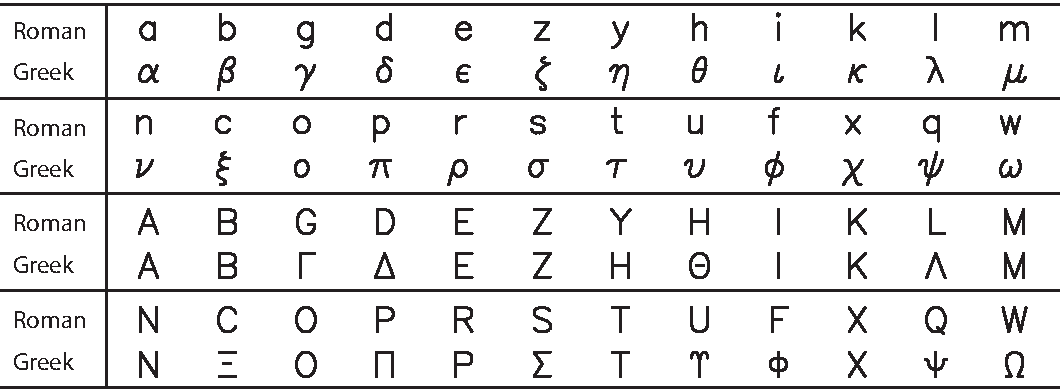
\includegraphics[width=5.0in]{greek.pdf}
  \caption[Roman to Greek Character Conversion]{Conversion for the string 
\vn{"{\B}g<r>"} where \vn{"<r>"} is a Roman character to the corresponding 
Greek character.}
\label{t:greek}
\end{table}

%-----------------------------------------------------------------
\subsection{Color Names}
\label{s:qp.color}

Possible settings for color parameters are:
\begin{example}
  White   (actually the background color)       Orange          
  Black   (actually the foreground color)       Yellow_Green    
  Red                                           Light_Green         
  Green                                         Navy_Blue       
  Blue                                          Purple          
  Cyan                                          Reddish_Purple  
  Magenta                                       Dark_Grey        
  Yellow                                        Light_Grey       
\end{example}
Color names are case insensitive.

%-----------------------------------------------------------------
\subsection{Line Pattern Names}
\label{s:qp.line.pat}

Possible settings for line patterns are:
\begin{example}
  solid      ! Solid line                 dotted     ! Dotted line             
  dashed     ! Dashed line                dash_dot3  ! Dash--dot--dot--dot line
  dash_dot   ! Dash--dot line
\end{example}
Pattern names are case insensitive.

%-----------------------------------------------------------------
\subsection{Fill Pattern Names}
\label{s:qp.fill.pat}

Possible fill pattern settings for symbols are:
\begin{example}
  solid_fill                    hatched           
  no_fill                       cross_hatched     
\end{example}
Fill pattern names are case insensitive.


\chapter{Optimization: Lattice Correction and Design}
\label{c:opti}

\index{optimization|hyperbf}

``\vn{Optimization}'' is the process of varying \vn{model} (\sref{s:lattice}) lattice parameters so
that a given set of properties are as close to a given set of ``desired'' values as
possible. Optimization problems generally fall into one of two categories. One category involves
``\vn{lattice correction}'' (\sref{s:lat.correction}). Problems in this category involve matching
the \vn{model} lattice to actual measured data. For example, orbit flattening involves varying
steerings in the \vn{model} lattice so that the orbit calculated from the \vn{model} lattice matches
the measured orbit. The steering strengths in the \vn{model} lattice can then be used to calculate
what changes are needed to correct the orbit in the actual machine.

The other category of optimization problems involves ``\vn{lattice design}'' (\sref{s:lat.design})
where lattice parameters are varied to achieve some set of ideal properties. For example, varying
sextupole magnet strengths in order to give maximum dynamic aperture.

Note: The \bmad and \tao tutorial (\sref{s:tutorial}) has examples of how to construct both lattice
correction and lattice design optimizations.

%------------------------------------------------------------------------
\section{Optimization Overview}
\label{s:opt.main}

Optimization involves ``\vn{data}'' and ``\vn{variables}''. \vn{Data} are the parameters to be
optimized. For example, orbit positions when flattening an orbit or the value of the beta function
at a certain point when designing a lattice. \vn{Variables} are what is to be varied which can be
steering strengths, magnet positions, etc. Any lattice parameters can be used with optimization as
long as varying the variables will affect the data. For example, orbit flattening is not restricted
to varying steerings and can be done by, say, varying magnet misalignments.

How data is organized in \tao is discussed in Chapter~\sref{c:data}. How to define datums in a \tao
initialization file is discussed in Section~\sref{s:init.data}. In brief, each datum has a set of
associated parameters. For example, each datum has ``\vn{model}'' and ``\vn{design}'' values which
are the values of the datum as calculated from the \vn{model} and \vn{design} lattices. Each datum
also has a ``\vn{measured}'' value which is set by the User. This value can be from an actual
measurement which is typical when doing lattice correction or may be the desired value of the datum
which is typical when doing lattice design. Which of the defined datums are varied during optimization
is controlled by setting the \vn{good_user} component of a datum (\sref{s:datum.opt}).

How variables are organized in \tao is discussed in Chapter~\sref{c:var}. How to define variables in
a \tao initialization file is discussed in Section~\sref{s:init.var}. In brief, like datums, each
variable has a number of associated parameters. For example, each variable has a ``\vn{model}''
value which controls the corresponding value or values (a variable can control multiple parameters
simultaneously) in the \vn{model} lattice. There are also ``\vn{low_lim}'' and ``\vn{high_lim}''
parameters that can be set by the User that are used to keep the variable \vn{model} value within a
given range.

Typically, optimization involves minimizing one or more ``objectives'' or ``merit functions''. \tao
itself implements ``single objective'' optimization where there is only one merit
function\footnote{For ``multiple objective'' optimization, there is a separate program called
\vn{moga} that can be used (\sref{s:other}).}. The general form of the merit function $\cal M$ in \tao
is
\begin{equation}
  {\cal M} \equiv 
    \sum_{i} w_i \, \bigl[ \delta D_i \bigr]^2 + 
    \sum_{j} w_j \, \bigl[ \delta V_j \bigr]^2
  \label{m1}
\end{equation}
The first term on the RHS is a sum over the \vn{data} and the second term is a sum over the
\vn{variables}.  The $w_i$ and $w_j$ are weights, specified by the User and stored in the
\vn{weight} component of a datum or variable. The value of $\delta D$ (\sref{s:del.d}) for a datum or
the value of $\delta V$ (\sref{s:del.v}) for a variable is put in the \vn{delta_merit} component of
the datum or variable. The contribution to the merit function, which is $[\delta D]^2$ for a datum
and $[\delta V]^2$ for a variable, is put in the \vn{merit} component of the datum or variable.

In some cases it might be desired a datum or variable's value. For example, maximizing the dynamic
aperture. In this case, the datum or variable weight $w$ needs to be set negative and the
contribution to the merit function will be negative. Note: The \vn{lmdif} optimizer
(\sref{s:tao.opti}) will not function correctly if there are negative weights.

In the case where it is not possible to calculate \vn{delta_merit} for a datum, for example, in the
case where a datum is associated with a Twiss parameter but the lattice is unstable, the value of
\vn{delta_merit} is set equal to the value of the datum's \vn{invalid} component. This is
useful for ensuring that the optimization does not get stuck in an unstable state. Additionally, the
following \vn{data_type} (\sref{s:data.types}) can be used to drive the optimization away from an
instability:
\begin{example}
  unstable.eigen
  unstable.eigen.a, .b, .c
  unstable.lattice
  unstable.orbit
\end{example}

There are a number of \vn{show} commands (\sref{s:show}) that can be used to show optimization
parameters:
\begin{example}
  show constraints    ! \sref{s:show.constraints} List of constraints 
  show data           ! \sref{s:show.data} Show data info
  show derivative     ! \sref{s:show.derivative} Show derivative info
  show merit          ! \sref{s:show.merit} Top contributors to the merit function
  show optimizer      ! \sref{s:show.optimizer} Optimizer parameters
  show variable       ! \sref{s:show.variables} Show variable info
\end{example}

%------------------------------------------------------------------------
\section{Calculation of $\delta D$ for a Datum}
\label{s:del.d}

The $\delta D$ terms in the merit function (\Eq{m1}) (the value of which is put in the datum's
\vn{delta_merit} component) are used to drive the \vn{model} lattice parameters towards a certain
set of desirable properties. How $\delta D$ is calculated for a given datum is determined, in part,
by the setting of the datum's \vn{merit_type} component. The possible settings of this component
are:
\begin{example}
  "target"                       ! Default
  "average"                      ! Uses evaluation range
  "integral"                     ! Uses evaluation range
  "rms"                          ! Uses evaluation range
  "min", "max"
  "abs_min", "abs_max"
  "max-min"                      ! Uses evaluation range
\end{example}
As noted, some of these settings need an \vn{evaluation range} (\sref{s:dat.eval}). An evaluation
range occurs when a datum's \vn{ele_start_name} is set and the evaluation range covers the region
from the lattice element identified by \vn{ele_start_name} and ending at the \vn{ele_name} element.
Note: It does not make sense for a datum with a \vn{data_type} that does not have an associated
evaluation element (for example, a datum with an emittance related \vn{data_type}), to have an
evaluation range. Therefore, for such datums, it is not possible to use any one of the four
\vn{merit_type} settings that use an evaluation range.

The calculation of $\delta D$ is a three step process. The first step is calculating the
\vn{model}, \vn{base} and \vn{design} values for a datum which are calculated from the \vn{model},
\vn{base}, and \vn{design} lattices. The first step calculation depends upon the setting of
\vn{merit_type} as well as whether there is an associated evaluation range.

For datums that do not have an evaluation range, the value of the datum's \vn{model}, \vn{base}, or
\vn{design} component is the appropriate value of the \vn{data_type}. For example, the $b$-mode
emittance for a \vn{data_type} setting of \vn{"emit.b"} or the horizontal dispersion (for
\vn{data_type} set to \vn{"eta.x"}) at the evaluation element (named by \vn{ele_name}). If there is
an associated reference element, the value will be modified by subtracting off the \vn{data_type}
value at the reference element. The exception is that for \vn{merit_type} set to \vn{"abs_min"} or
\vn{"abs_max"}, the absolute value is taken (this is done after any reference value is subtracted).

For datums that do have an an evaluation region, the \vn{model}, \vn{base}, or \vn{design} datum values
are computed as described below. In all cases, if there is an associated reference element, the value
will be modified by subtracting off the \vn{data_type} value at the reference element.
\begin{description}[itemsep=0pt,topsep=0pt]
%
\item["target"] \Newline
With \vn{merit_type} set to\vn{"target"}, an evaluation range is not permitted since it does not
make sense to have one.
%
\item["average"] \Newline
With \vn{"average"} as the \vn{merit_type}, the value is the mean of the
\vn{data_type} over the evaluation region. This is just the integral normalized by the length of the
region. To save time, the data is only evaluated at the ends of elements
and the average is evaluated assuming linear variation between points.
%
\item["integral"] \Newline
With \vn{"integral"} as the \vn{merit_type}, the value is the integral of the \vn{data_type} over
the evaluation region. To save time, the data is only evaluated at the ends of elements and the
integral is evaluated assuming linear variation between points.
%
\item["min" or "max"] \Newline
With \vn{"min"} or \vn{"max"} as the \vn{merit_type}, the value
is the minimum or maximum value of the \vn{data_type} over the evaluation region.
%
\item["abs_min" or "abs_max"] \Newline
With \vn{"abs_min"} or \vn{"abs_max"} as the \vn{merit_type}, the value for a lattice is the minimum
or maximum value of the absolute value of the \vn{data_type} over the evaluation region.
%
\item["max-min"] \Newline
With \vn{"max-min"} as the \vn{merit_type}, the value for a lattice is the maximum value of the
\vn{data_type} over the evaluation region minus the minimum value over the evaluation region.
%
\item["rms"] \Newline
With \vn{"rms"} as the \vn{merit_type}, the value is the RMS of the
\vn{data_type} over the evaluation region. To save time, the data is only evaluated at the ends of elements
and the RMS is evaluated assuming linear variation between points.
\end{description}

  %
\begin{table}[tb] 
\centering 
{\tt
\begin{tabular}{lll} \toprule
  \vn{Opt_with_ref} & \vn{Opt_with_base} & Composite Value Expression \\ \midrule
  F & F & model - meas                    \\
  F & T & model - meas - base             \\
  T & F & (model - meas) - (design - ref) \\
  T & T & (model - meas) - (base - ref)   \\
\bottomrule
\end{tabular}
}
  \caption[Expression used to combine the values of \vn{model}, \vn{base}, \vn{design}, \vn{meas}, and
\vn{ref} into one ``composite'' value.]{
The expression used to combine the values of \vn{model}, \vn{base}, \vn{design}, \vn{meas}, and
\vn{ref} into one ``composite'' value is determined by the settings of \vn{opt_with_ref} and
\vn{opt_with_base} global parameters. These expressions are the same as Table~\ref{t:delta.v}.
  }
\label{t:delta.d}
\end{table}
  % 

After a datum's \vn{model}, \vn{base} and \vn{design} values are calculated, these values are
combined together along with the \vn{meas} and \vn{ref} values set by the User\footnote
  {
keep in mind that the \vn{ref} component is different from the \vn{ele_ref_name}
component (\sref{s:data.anatomy}). \vn{ele_ref_name} is used to set a reference element which is used
when evaluating \vn{model}, \vn{base}, and \vn{design} values (\sref{s:lat.correction}). The value of
the \vn{ref} component is set by the user.
  }. 
The formula used to combine these values into one ``\vn{composite}'' value is determined by the
setting of two global logicals \vn{opt_with_ref} and \vn{opt_with_base}. These parameters are in the
\vn{tao_global_struct} structure (\sref{s:tao.global.struct}). Table~\ref{t:delta.d} shows the
expressions.

After the \vn{composite} value is calculated, $\delta D$ will be set equal to the \vn{composite} value
except if the \vn{merit_type} is \vn{"min"}, \vn{"max"}, \vn{"abs_min"}, or \vn{"abs_max"}.  For 
\vn{"min"} and \vn{"abs_min"}, $\delta D$ will be
\begin{equation}
  \delta D = 
  \begin{cases}
    0 & \tv{composite} > 0 \\
    \tv{composite} & \tv{otherwise}
  \end{cases}
\end{equation}
That is, the datum only contributes to the merit function if the \vn{composite} is value is negative.
For \vn{"max"} and \vn{"abs_max"}, $\delta D$ will be
\begin{equation}
  \delta D = 
  \begin{cases}
    0 & \tv{composite} < 0 \\
    \tv{composite} & \tv{otherwise}
  \end{cases}
\end{equation}
That is, the datum only contributes to the merit function if the \vn{composite} is value is positive.

%------------------------------------------------------------------------
\section{Calculation of $\delta V$ for a Variable}
\label{s:del.v}

The $\delta V$ terms in the merit function (\Eq{m1}) serve one of two purposes. Such terms can be
used to keep variables within certain limits or can be used to guide the optimization towards a
solution where a variable has a certain value. How $\delta V$ is calculated for a given variable is
determined by the setting of the variable's \vn{merit_type} component. This component can
have one of two values:
\begin{example}
  "limit"     ! Default
  "target"
\end{example}

For \vn{merit_type} set to \vn{"limit"}, the value of $\delta V$ is determined by the setting of the
variable's \vn{high_lim} and \vn{low_lim} components. If not explicitly set, \vn{high_lim} defaults
to $10^{30}$ and \vn{low_lim} defaults to $-10^{30}$. The value of $\delta V$ in this case is
\begin{equation}
  \delta V = 
  \begin{cases}
    \tv{model} - \tv{high_lim} & \tv{model} > \tv{high_lim} \\
    \tv{model} - \tv{low_lim} & \tv{model} > \tv{low_lim} \\
    0 & \tv{otherwise}
  \end{cases}
\end{equation}

Note: When running the optimizer, if the parameter \vn{global%var_limits_on} (\sref{s:globals}) is
\vn{True}, and if the \vn{model} value of a variable is outside of the range set by the limits, \tao
will do two things: First, the \vn{model} value of the variable will be set to the value of the
nearest limit and, second, the variable's \vn{good_user} parameter (\sref{c:var}) is set to
False so that no further variation by the optimizer is done. This is done independent of the setting
of \vn{merit_type} for the variable and independent of whether the variable is being used in the
optimization. Sometimes it is convenient to not set the \vn{model} value to the nearest limit for
variables that are not being used in the optimization. In this case, the global parameter
\vn{global%only_limit_opt_vars} may be set to \vn{True}.  If this is done, only variables that the
optimizer is allowed to vary are restricted.

Note: The \vn{global%optimizer_var_limit_warn} parameter controls whether a warning is printed when a
variable value goes past a limit.  The default is \vn{True}.

  %
\begin{table}[ht] 
\centering 
{\tt
\begin{tabular}{lll} \toprule
  \vn{Opt_with_ref} & \vn{Opt_with_base} & \vn{Delta_Merit} ($\delta V$) Formula \\ \midrule
  F & F & model - meas                    \\
  F & T & model - meas - base             \\
  T & F & (model - meas) - (design - ref) \\
  T & T & (model - meas) - (base - ref)   \\
\bottomrule
\end{tabular}
}
  \caption[The formulas for evaluating $\delta V$ used in the Merit function.]{
When \vn{merit_type} is set to \vn{"target"}, the formula for evaluating $\delta V$ is determined by
the settings of \vn{opt_with_ref} and \vn{opt_with_base} global parameters as shown in the
table. These expressions are the same as Table~\ref{t:delta.d}.
  }
\label{t:delta.v}
\end{table}
  % 
For \vn{merit_type} set to \vn{"target"}, the formula used to compute $\delta V$ is determined by
the setting of two global logicals \vn{opt_with_ref} and \vn{opt_with_base}. These parameters are in
the \vn{tao_global_struct} structure (\sref{s:tao.global.struct}). Table~\ref{t:delta.v} shows the
expressions used to evaluate $\delta V$
In the table, \vn{model}, \vn{base} and \vn{design} are the values for the variable as set in the
\vn{model}, \vn{base}, and \vn{design} lattices, and the variable's \vn{meas} and \vn{ref} values
are set by the User. 

%------------------------------------------------------------------------
\section{Lattice Corrections}
\label{s:lat.correction}
\index{modeling data}
\index{lattice corrections}
\index{optimization!merit function}

Lattice correction is the process of varying a set of parameters in a machine achieve some desirable
state.  Typically, there are three stages. First there is a measurement. After this, corrections can
be calculated (the optimization stage). Finally, the calculated corrections are loaded into the
machine.

There are several variations of how optimization is done. To make the discussion concrete, the
case where a beta function measurement is used to calculate quadrupole \vn{K1} strength changes to
correct the machine optics is considered.\footnote
  { 
The beta function can be measured, for example, by pinging the
beam and observing the oscillations at the beam position monitors.
  }.
In this case, both data and variables will have their \vn{merit_type} set to \vn{"target"}, the
global \vn{opt_with_ref} and \vn{opt_with_base} will be False. With this, $\delta D$ and $\delta V$
in \Eq{m1} will be
\begin{align}
  \delta &\tv{D} = \tv{model_beta} - \tv{meas_beta} \CRNO
  \delta &\tv{V} = \tv{model_K1} - \tv{meas_K1}
  \label{dd1}
\end{align}
The \vn{meas_beta} data values will is the measured beta function and the variable \vn{meas_K1}
values will be the measured quadrupole \vn{K1} at the time the data was taken. The quadrupole
\vn{K1} could be measured from, for example, from the currents through the quadrupoles combined with
known current to field calibrations. The $\delta V_j$ terms in the merit function prevents
degeneracies (or near degeneracies) in the problem which would allow \tao to find solutions where
\vn{model_beta} matches \vn{meas_beta} with the \vn{model_k1} strengths having ``unphysical'' values
far from the measured strengths. The weights $w_i$ and $w_j$ in \Eq{m1} need to be set depending
upon how accurate the measured data is relative to the measured magnet strengths.

If the fit is good, the beta function is corrected by changing the
quadrupole strengths in the machine by an amount \vn{dK1} given by
\begin{example}
  dK1 = design_K1 - model_K1
\end{example}
where \vn{design_K1} is the \vn{design} value for the quadrupole strengths. The equation for
\vn{dK1} is derived using the following logic: Once a fit to the measured data has been made, the
\vn{model} lattice corresponds, more or less, to the actual state of the machine. On the other hand,
the desired state is given by the \vn{design} lattice . Thus the difference, \vn{design - model},
represents the desired state minus the actual state. The final state after the
correction will be
\begin{example}
  Final_State = Initial_State + Change
              = Actual_State + (Desired_State - Actual_State)
              = Desired_State
\end{example}
which is what is wanted.

Notice that the fitting process is independent of the strengths of the parameters in the
\vn{design} lattice. That is, the fit involves the actual machine state independent of what the
desired state is. It is not until the values needed for the correction are computed that the
parameter strengths in the \vn{design} lattice come into play.

To the extent that the measured beta function can be well fit determines the extent to which the
beta function can be corrected. For example, if an unwanted quadrupole error is generated by some
element at a spot that is far from any correctors (quadrupoles that can vary), it will not be possible to
fit the measured beta function well and it will not be possible to make a good correction. If, on
the other hand, an unwanted error is generated next to one corrector, the measured beta function can
be well fit and the \vn{model} lattice will have a strength change from the \vn{design} for that one
corrector. Varying that one corrector can then cancel out the unwanted kick.

Another point is that the correction algorithm will work with varying any set of parameters as long
as the variation in the parameters affect the \vn{model} data. Thus an analysis can be made of the
beam orbit using dipole rolls and/or quadrupole offsets as variables or any combination thereof. If
the fit is good, rolling the dipoles and moving the quadrupoles will correct the orbit. With \tao,
the User has complete freedom to vary any parameters in the fitting process.

Typically, at the start of the fit, the \vn{model} lattice is, by default, equal to the \vn{design}
lattice but this is not necessary. Generally, the actual machine state is near enough to the
\vn{design} machine state so that the machine will behave roughly linearly with the variation in the
parameters (if the machine parameters are far from the design values, it may not be possible to
store beam to take a measurement in the first place). This means that there will be only one minimum
merit function state so that the parameter values (quadrupole strengths in this case) at the end of
the fit are independent of the starting state. To put this in other terms, the User generally does
not have to worry about the initial state of the \vn{model} at the start of a fit. This is in
contrast to lattice design (\sref{s:lat.design}) where there are typically many local minima and it
can take days of work to find a good operating point. With lattice correction, on the other hand,
the near linear nature of the problem means that finding a solution in a machine with hundreds of
correctors and hundreds of BPM readings can be done in seconds with the \vn{lm} or \vn{lmdif}
optimizers (\sref{s:tao.opti}).

%------------------------------------------------------------------------
\section{Lattice Design}
\label{s:lat.design}
\index{optimization!lattice design}
\index{optimization!constraints}

Lattice design is the process of calculating \vn{variable} strengths to meet a number of criteria
called constraints. For example, one constraint could be that the beta function in some part of the
lattice not exceed a certain value or a constraint is used to keep the \vn{model} at a certain desired
value. To keep the nomenclature consistent, the desired value is labeled \vn{meas} even though it is not
a ``measured'' value.

Lattice design is an art in that there is no known algorithm that will guarantee that a global
minimum has been found. And indeed, there is no known general procedure for checking that a given
minimum is the global minimum. \tao has one optimizer for global minimum searching and that is the
\vn{de} optimizer (\sref{s:tao.opti}). Typical strategies involve using the \vn{de} optimizer to
find a minimum, then using the \vn{lm} or \vn{lmdif} optimizer to refine the answer, and then
switching back to the \vn{de} optimizer to see if a better minimum can be found. This is repeated
while varying the \vn{de} parameters and/or weights in the merit function (\Eq{m1}).

As an alternative, there is a \bmad based program separate from \tao called \vn{moga} that can be
used (\sref{s:other}). This program implements multi objective optimization.

%------------------------------------------------------------------------
\section{Optimizers in Tao}
\label{s:tao.opti}
\index{optimization!optimizer}

The algorithm used to vary the \vn{model} variables to minimize \vn{M} is called an \vn{optimizer}.
In \vn{command line mode} the \vn{run} command is used to invoke an \vn{optimizer}. In \vn{single
mode} the \vn{g} key starts an optimizer. In both modes the period key (\vn{``.''}) stops the
optimization (however, the \vn{global%optimizer_allow_user_abort} parameter (\sref{s:globals}) can
be set to False to prevent this). Running an optimizer is also called ``fitting'' since one is
trying to get the \vn{model} data to be equal to the \vn{measured} data. With orbits this is also
called ``flattening'' since one generally wants to end up with an orbit that is on--axis.

The optimizer that is used can be defined when using the \vn{run} command but the default optimizer
can be set in the \tao input file by setting the \vn{global%optimizer} component (\sref{s:globals}).

When the optimizer is run in \tao, the optimizer, after it initializes itself, takes a number of
\vn{cycles}. Each cycle consists of changing the values of the variables the optimizer is allowed to
change. The number of steps that the optimizer will take is determined by the parameter
\vn{global%n_opti_cycles} (\sref{s:globals}). When the optimizer initializes itself and goes through
\vn{global%n_opti_cycles}, it is said to have gone through one \vn{loop}. After going through
through \vn{global%n_opti_loops} loops, the optimizer will automatically stop.  To immediately stop
the optimizer the period key \vn{``.''} may be pressed. Note: In \vn{single_mode} (\sref{c:single}),
\vn{n_opti_loops} is ignored and the optimizer will loop forever.

There are currently three optimizers that can be used: 
  \begin{description}
  \index{lm optimizer}
  \item{\vn{lm}} \Newline
\vn{lm} is an optimizer based upon the Levenburg-Marquardt algorithm
\cite{b:nr}. This algorithm looks at the local derivative matrix of \vn{dData/dVariable} and
takes steps in variable space accordingly. The derivative matrix is calculated beforehand by varying
all the variables by an amount set by the variable's \vn{step} component (\sref{s:init.var}). The
\vn{step} size should be chosen large enough so that round-off errors will not make computation of
the derivatives inaccurate but the step size should not be so large that the derivatives are
effected by nonlinearities. By default, the derivative matrix will be recalculated each \vn{loop}
but this can be changed by setting the \vn{global%derivative_recalc} global parameter
(\sref{s:globals}). The reason to not recalculate the derivative matrix is one of time.  However, if
the calculated derivative matrix is not accurate (that is, if the variables have changed enough from
the last time the matrix was calculated and the nonlinearities in the lattice are large enough), the
\vn{lm} optimizer will not work very well.  In any case, this method will only find local minimum.
When running with \vn{lm}, the value of a parameter called \vn{a_lambda} will be printed. This
``damping factor'', which is always positive definite, is a measure of how well the variation of the
$\delta D_i$ terms with respect to the variables in \Eq{m1} matches the computed derivative matrix.
A small \vn{a_lambda}, much less than one, indicates good agreement while a larger \vn{a_lambda},
much greater than one, means that there is a mismatch. If \vn{a_lambda} is large, the optimizer will
not be able to make much progress. There are several reasons for a large \vn{a_lambda}. First, the
working point may have shifted enough so that the derivative matrix needs to be recalculated. If
recalculating the derivative matrix does not fix the problem, it may be that one or more variable
\vn{step} sizes are either too small or two large. If the value of \vn{step} is too small for a
variable, round-off error can cause the calculation of the variable's derivatives to be off. If the
value of the \vn{step} is too large, nonlinearities can throw off the derivative calculation. To
test if the step size is set correctly first use the \vn{show merit -derivative} command to see what
variables have the largest \vn{dMerit/dVariable} values as computed from the derivative
matrix. [Note: Generally the best thing is to concentrate on the variables with the largest
derivatives since these give the ``most bang for the buck''.] These values should be small when at
the true merit function minimum. The \vn{change variable} command can now be used with varying step
sizes to see if the actual \vn{dMerit/dVariable} change matches this. The output from the
\vn{change} command will show the \vn{dMerit/dVariable} value computed from varying the variable by
the amount given in the change command. If the two do not agree, there may be a problem. Warning! At
the $\cal M$ minimum the value of \vn{dMerit/dVariable} is very sensitive to the value of the
variables. To not get fooled, move away the minimum. For more information on \vn{a_lambda}, see the
Wikipedia article on the ``\vn{Levenberg–Marquardt algorithm}''. In this article the variable is
denoted $\lambda$.
  \index{lmdif optimizer}
  \item{\vn{lmdif}} \Newline
The \vn{lmdif} optimizer is like the \vn{lm} optimizer except that it builds up the information it
needs on the derivative matrix by initially taking small steps over the first \vn{n} cycles where
\vn{n} is the number of variables. The advantage of this is that you do not have to set a \vn{step}
size for the variables. The disadvantage is that for \vn{lmdif} to be useful, the number of
\vn{cycles} (set by \vn{set global n_cycles =<XXX>}) must be greater than the number of
variables. Again, like \vn{lm}, this method will only find local minimum.
  \index{de optimizer}
  \item{\vn{de}} \Newline
The \vn{de} optimizer stands for \vn{differential evolution}\cite{b:de}. The advantage of this
optimizer is that it looks for global minimum. The disadvantage is that it is slow to find the
bottom of a local minimum. A good strategy sometimes when trying to find a global minimum is to use
\vn{de} in combination with \vn{lm} or \vn{lmdif} one after the other. One important parameter with
the \vn{de} optimizer is the \vn{step} size. A larger step size means that the optimizer will tend
to explore larger areas of variable space but the trade off is that this will make it harder to find
minimum in the locally. One good strategy is to vary the \vn{step} size to see what is
effective. Remember, the optimal step size will be different for different problems and for
different starting points. The \vn{step} size that is appropriate of the \vn{de} optimizer will, in
general, be different from the \vn{step} size for the \vn{lm} optimizer. For this reason, and to
facilitate changing the step size, the actual step size used by the \vn{de} optimizer is the step
size given by a variable's \vn{step} component multiplied by the global variable
\vn{global%de_lm_step_ratio}. This global variable can be varied using the \vn{set} command
(\sref{s:set}). The number of trial solutions used in the optimization is
\begin{example}
  population = number_of_variables * global%de_var_to_population_factor
\end{example}
There are also a number of parameters that can be set that will affect how the optimizer works. See
Section~\sref{s:globals} for more details.
  \index{svd optimizer}
  \item{\vn{svd}} \Newline
The \vn{svd} optimizer uses a singular value decomposition calculation. With the \vn{svd}
optimizer, the setting of the \vn{global%n_opti_cycles} parameter is ignored. One optimization loop
consists of applying svd to the derivative matrix to locate a new set of variable values.  If the
merit function decreases with the new set, the new values are retained and the optimization loop is
finished. If the merit function increases, and if the global variable
\vn{global%svd_retreat_on_merit_increase} is True (the default), the variables are set to the
original variable settings. In either case, an increasing merit function will stop the execution of
additional loops.

The \vn{global%svd_cutoff} variable can be used to vary the cutoff that SVD uses to decide what
eigenvalues are singular.
  \end{description}

%------------------------------------------------------------------------
\section{Optimization Troubleshooting Tips}
\label{s:opt.trouble}
\index{optimization troubleshooting}

Optimization can be tricky. There are many parameters that affect the optimization and often it
comes down to trial and error to find an acceptable an acceptable solution. And even in expert
hands, optimizations can take days. The following are some tips if there are problems with an
optimization.

\begin{description}
%
\item[Show commands] \Newline
Commands that can be used to view optimizer parameters are:
\begin{example}
  show constraints
  show data
  show derivative
  show merit
  show optimizer
  show variable
\end{example}
%
\item[Set the optimizer to run longer] \Newline
One quick thing to do is to increase the number of optimization loops and/or optimization cycles:
\begin{example}
	set global n_opti_loops = 30
	set global n_opti_cycles = 50
\end{example}
The \vn{show optimizer} (\sref{s:show.optimizer}) command will show global parameters
associated with optimizations.
%
\item[Check merit function and weights] \Newline
One of the first things to check is the merit function, the top contributors can be seen with the
command \vn{show merit} (\sref{s:show.merit}). And individual contributions can be viewed using the
\vn{show variable} and \vn{show data} commands. If the weight of an individual datum is too small,
the optimizer will tend to ignore it. So one trick is to raise the weights for datums that are not
being well optimized. When running \tao this is done with the \vn{data data} command. For example:
\begin{example}
  set data twiss.a[1:2]|weight = 100*twiss.a[1:2]|weight
\end{example}
This example will increase the weight of datums \vn{twiss.a[1]} and \vn{twiss.a[2]} by a factor of
100.
%
\item[Check step size] \Newline
If using an optimizer that uses the derivative matrix (\vn{lm}, \vn{geodesic_lm} and \vn{svd}
optimizers), The variable \vn{step} sizes that are used to calculate the derivative should be
checked to make sure that the \vn{step} is not too small so that round-off is a problem but yet not
too large so that nonlinearities make the calculation inaccurate. One way to check that the step
size is adequate for a given variable is to vary the variable using the command \vn{change var}
(\sref{s:change}). This command will print out the the change in the merit function per change in
variable which can be compared to the derivatives as shown with the \vn{show merit -derivative}
(\sref{s:show.merit}) or the \vn{show derivative} (\sref{s:show.derivative}) command.
%
\item[Rotate optimizer usage] \Newline
Problems generally occur when there are many local minima. In this case, the \vn{de} optimizer
(\sref{s:tao.opti}) should be tried. This optimizer has several parameters which will need to be
varied by trial and error to find values that are suitable for the problem at hand. Optimization
strategies here include doing multiple optimizations one after another using the \vn{de} optimizer
every other optimization interlaced with one of the other optimizers. Also varying the merit
function weights between optimizations can help guide the optimization process towards an acceptable
solution.
\item[Use a non-\tao optimizer]
Using, for example, a Python based optimizer interfaced to \tao is possible. There is also the \vn{moga}
program which implements multi-objective optimization.
\end{description}


%------------------------------------------------------------------------
%++++++++++++++++++++++++++++++++++++++++++++++++++++++++++++++++++++++++
%------------------------------------------------------------------------

\endinput

\etcetc...

%------------------------------------------------------------------------
\section{Common Root Lattice (CRL) Analysis}
\label{s:crl}
\index{common root lattice}

Some data analysis problems involve varying variables in a both the \vn{model} and \vn{base}
lattices simultaneously. Such is the case with Orbit Response Matrix (\vn{ORM})
analysis\cite{b:orm}. With \vn{ORM}, the analysis starts with a set of difference orbits. A given
difference orbit is generated by varying a given steering by a known amount and the steering varied
is different for different difference orbits. Typically, The number $N$ of difference orbits is
equal to the number of steering elements in the machine. In \tao, this will result in the creation
of $N$ universes, one for each difference measurement. The \vn{model} lattice in a universe will
correspond to the machine with the corresponding steering set to what it was when the data was
taken. Conversely, the \vn{base} lattices in all the universes all correspond to the common
condition without any steering variation.

In \tao, this arrangement is called \vn{Common Root Lattice} (\vn{CRL}) analysis. To do a CRL
analysis, the \vn{common_lattice} switch must be set at initialization time (\sref{s:init.lat}).
With \vn{CRL}, \tao will set up a \vn{``common''} universe with index 0.  The \vn{model} lattice of
this common universe will be used as the \vn{base} lattice for all universes.

The variables (fit parameters) in a \vn{CRL} analysis can be divided into two classes. One class
consists of the parameters that were varied to get the data of the different universes. With
\vn{ORM}, these are the steering strengths. At initialization (\sref{s:init.var}), variables must be
set up that control these parameters. A single variable will control that particular parameter in a
particular universe, that was varied to create the data for that universe.

The second class of variables consists of everything that is to be varied in the common root
lattice. With \vn{ORM}, this generally will include such things as quadrupole and BPM error tilts,
etc. That is, parameters that did {\em not} change during data taking. The \tao variables that are
created for these parameters will control parameters of the \vn{model} lattice in the common
universe.

To cut down on memory usage when using \vn{CRL} (the number of data sets, hence the number of
universes, can be very large), \tao does not, except for the common \vn{model} lattice, reserve
separate memory for each \vn{model} lattice. Rather, it reserves memory for a single
\vn{``working''} lattice and the \vn{model} lattice for a particular universe is created by first
copying the common \vn{base} lattice to the \vn{working} lattice and then applying the variable(s)
(a steering in the case of \vn{ORM}) appropriate for that universe.  As a result, except for the
common \vn{model} lattice, it is not possible to vary a parameter of a \vn{model} lattice unless
that parameter has a \tao variable that associated with it. The \vn{change} command
(\sref{s:change}) is thus restricted to always vary parameters in the common \vn{model} lattice.

With \vn{CRL}, the \vn{opt_with_base} and \vn{opt_with_ref} (\sref{s:del.d}) global
logicals are generally set to True. Since \vn{opt_with_base}, and \vn{opt_with_ref} do not make
sense when applied to the data in the common universe, The contribution to the merit function from
data in this universe is always calculated as if \vn{opt_with_base} and \vn{opt_with_ref} were set
to False.

With \vn{opt_with_base} set to True, the \vn{base} value for a datum is evaluated by looking for a
corresponding datum in the common universe and using its \vn{model} value. To simplify the
bookkeeping, it is assumed that the structure of the data arrays is identical from universe to
universe. That is, the \vn{show data} command gives identical results independent of the default
universe.


Re: opt_with_ref and opt_with_base global parameters: An exception occurs when using a \vn{common
root lattice} (\sref{s:crl}). In this case, the common universe does not have base or reference
values associated with it. Thus all data and variables that are associated with the common universe
calculate their \vn{delta} as if both \vn{opt_with_ref} and \vn{opt_with_base} were set to
\vn{False}.


\chapter{Wave Analysis}
\label{c:wave}

%----------------------------------------------------------------
\section{General Description}
\label{s:wave.general}

A ``wave analysis'' is method for finding isolated ``kick errors'' in a machine by analyzing the
appropriate data. Types of data that can be analyzed and the associated error type is shown in
Table~\ref{t:wave0}.

The analysis works on difference quantities. For example, the difference between measurement and
theory or the difference between two measurements, etc. Orbit and vertical dispersion measurements
are the exception here since an analysis of, say, just an orbit measurement can be considered to be
the difference between the measurement and a perfectly flat (zero) orbit.

\begin{table}[h]
\centering{\tt
\begin{tabular}{ll} \toprule
  {\it Measurement Type}     & {\it Error Type}           \\ \midrule
  Orbit                      & Steering errors            \\
  Betatron phase differences & Quadrupolar errors         \\
  Beta function differences  & Quadrupolar errors         \\
  Coupling                   & Skew quadrupolar errors    \\
  Dispersion differences     & Sextupole errors           \\ \bottomrule
\end{tabular}}
\caption[Wave measurement types.]  {Types of measurements that can be used in a wave analysis and
the types of errors that can be diagnosed.}  
\label{t:wave0}
\end{table}

\begin{figure}[t]
  \centering
  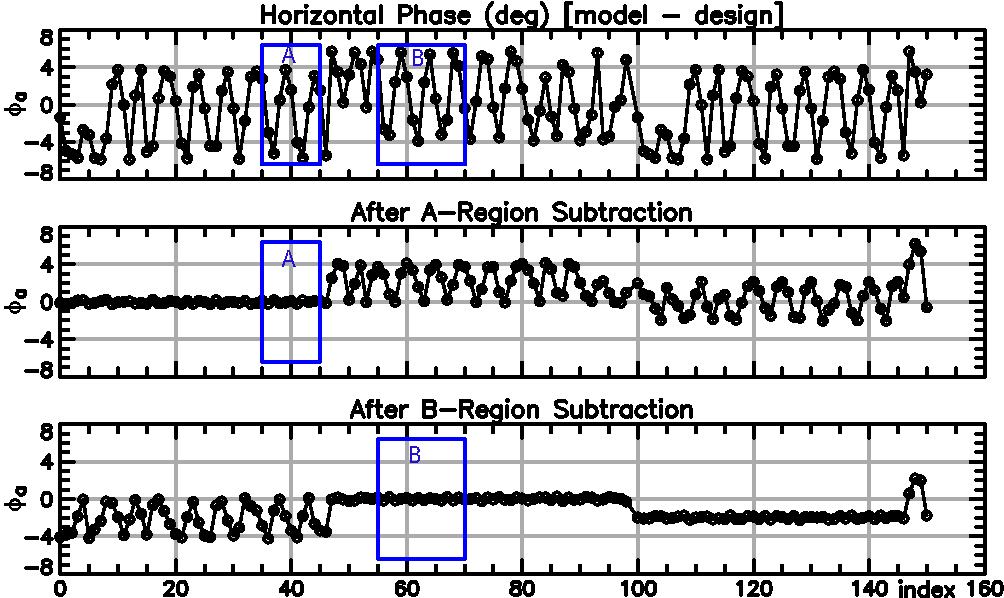
\includegraphics[width=6in]{wave.pdf}
  \caption[Example wave analysis.]
{Example wave analysis for betatron phase data.}
  \label{f:wave}
\end{figure}

The formulation of the wave analysis for quadrupolar and skew quadrupolar errors is presented by
Sagan\cite{b:wave}. Although not discussed in the paper, the wave analysis for orbit and dispersion
measurements is similar to analysis in the paper.

The wave analysis is similar for all the measurement types. How the wave analysis works is
illustrated in Figure~\ref{f:wave}.  Figure~\ref{f:wave}a shows the difference between \vn{model}
and \vn{design} values for the $a$-mode betatron phase for the Cornell's Cesr storage ring. In this
example, one quadrupole in the model has been varied from it's design value. The horizontal axis is
the detector index.

For the wave analysis, two regions of the machine, labeled $A$ and $B$ in the figure, are chosen
(more on this later). For each region in turn, the data in that region is fit using a functional
form that assumes that there are no kick errors in the regions.  For phase differences, this
functional form is
\begin{equation}
  \delta \phi(s) = D \, \sin(2 \, \phi(s) + \phi_0) + C
  \label{xabps}
\end{equation}
where $\phi$ is the phase advance and the quantities $C$, $D$ and $\phi_0$ are varied to give the
best fit.  Once $C$, $D$, and $\phi_0$ are fixed, \Eq{xabps} can be evaluated at any
point. Figure~\ref{f:wave}b shows the orbit of \ref{f:wave}a with the fit to the $A$ region
subtracted off. Similarly, Figure~\ref{f:wave}c shows the orbit of Figure~\ref{f:wave}a with the fit
to the $B$ region subtracted off. Concentrating on Figure~\ref{f:wave}b, since there are no kick
errors in the $A$ region, the fit is very good and hence the difference between the data and the fit
is nearly zero. Moving to the right from the $A$ region in Figure~\ref{f:wave}b, this difference is
nearly zero up to where the assumption of no kick errors is violated. That is, at the location of
the quadrupole error near detector 47. Similarly, since there are no kick errors in region $B$, the
difference between the data and the $B$ region fit is nearly zero in Figure~\ref{f:wave}c and this
remains true moving leftward from region $B$ up to the quadrupole near detector 47.

By taking the fitted values for $C$, $D$, and $\phi_0$ for the regions $A$ and $B$, the point
between the regions where the kick is generated and the amplitude of the kick can be
calculated. This calculation is similar to that used to find quadrupolar errors from beta data
instead of phase data. The one difference is a factor of 2 that appears in the beta calculation due
to the fact that a freely propagating beta wave oscillates at $2\phi(s)$.

The success of the wave analysis in finding a kick error depends upon whether there are regions of
sufficient size on both sides of the kick that are kick error free. That is, whether the kick error
is ``isolated''. The locations of the $A$ and $B$ regions are set by the user and the general
strategy is to try to find, by varying the location of the regions, locations where the data is well
fit within the regions. The data is well fit if the difference between data and fit is small
compared to the data itself. If there are multiple isolated kick errors, then each error in turn can
be bracketed and analyzed. If there are multiple errors so close together that they cannot be
resolved, this will throw off the analysis, but it may still be possible to give bounds for the
location where the kicks are at and an ``effective'' kick amplitude can be calculated.

For circular machines, to be able to analyze kicks near the beginning or end of the lattice, the
wave analysis can be done by ``wrapping'' the data past the end of the lattice for another 1/2
turn. This is illustrated in Figure~\ref{f:wave}. In the Cesr machine, there are approximately 100
detectors labeled from 0 to 99.  The detectors from 100 to 150 are just the detectors from 0 to 50
shifted by 100. Thus, for example, the detector labeled 132 in the figure is actually detector 32.

%----------------------------------------------------------------
\section{Wave Analysis in Tao}
\label{s:wave.tao}

Performing a wave analysis in \tao is a three step process:
\begin{example}
  1) Plot the data to be analyzed.
  2) Use the \vn{wave} command to select the data.
  3) Use the \vn{set wave} command to vary the fit regions.
\end{example}

In general, the accuracy of the wave analysis depends upon the accuracy with which the beta function
and phase advances are known in the baseline lattice used. \tao uses the \vn{model} lattice for the
baseline. If possible, One strategy to improve the accuracy of the wave analysis is first use a
measurement to calculate what the quadrupole strengths in the \vn{model} lattice should be. Possible
measurements that can give this information include an orbit response matrix (ORM) analysis, fits to
beta or betatron phase measurements, etc.

%----------------------------------------------------------------
\section{Preparing the Data} 
\label{s:wave.data}

At present (due to limited manpower to do the coding), the wave analysis is restricted to data that
is stored in a \vn{d1_data} array (\sref{c:data}). That is, the plotted curve to be analyzed must
have its \vn{data_type} parameter set to \vn{``data''} (\sref{s:init.data}). The possible data types
that can be analyzed are:
\begin{example}
  orbit.x, orbit.y
  beta.a,  beta.b
  phase.a, phase.b
  eta.x, eta.y
  cbar.11, cbar.12, cbar.21      ! Analysis not possible for cbar.21
  ping_a.amp_x, ping_a.phase_x
  ping_a.sin_y, ping_a.cos_y
  ping_b.amp_y, ping_b.phase_y
  ping_b.sin_x, ping_b.cos_x
\end{example}
The curve to be analyzed must be visible. Any combination of data components may be used:. "meas",
"meas-ref", "model", etc.

If data from a circular machine is being analyzed, the data is wrapped past the end of the lattice
for another 1/2 turn. The translation from the data index in the wrapped section to the first 1/2
section of the lattice is determined by the values of \vn{ix_min_data} and \vn{ix_max_data} of the
\vn{d1_data} array under consideration (\sref{s:init.data}):
\begin{example}
  index_wrap \(\longrightarrow\) index_wrap - (ix_max_data - ix_min_data + 1)
\end{example}
For example, for the Cesr example in the previous section, \vn{ix_min_data} was 0 and
\vn{ix_max_data} was 99 to the translation was
\begin{example}
  index_wrap \(\longrightarrow\) index_wrap - 100
\end{example}

%----------------------------------------------------------------
\section{Wave Analysis Commands and Output}
\label{s:wave.cmd.out}

The \vn{wave} command (\sref{s:wave}) sets which plotted data curve is used for the wave
analysis. The \vn{set wave} command (\sref{s:set}) is used for setting the $A$ and $B$ region
locations. Finally the \vn{show wave} command (\sref{s:show}) prints analysis results.

Example wave analysis output with \vn{show wave}:
\begin{example}
  ix_a:  35  45
  ix_b:  55  70
  A Region Sigma_Fit/Amp_Fit:     0.018
  B Region Sigma_Fit/Amp_Fit:     0.015
  Sigma_Kick/Kick:    0.013
  Sigma_phi:          0.019
  Chi_C:              0.037 [Figure of Merit]

  Normalized Kick = k * l * beta [dimensionless]
     where k = quadrupole gradient [rad/m^2].
  After Dat#     Norm_K       phi
         46      0.0705    30.431
         49      0.0705    33.573
         53      0.0705    36.715
\end{example}
This output is for analysis of betatron phase data but the output for other types of data is
similar.  The first two lines of the output show where the $A$ and $B$ regions are. The next two
lines show $\sigma_{a}/A_a$ and $\sigma_{b}/A_b$ where $\sigma_a$ and $\sigma_b$ are given by
Eq.~(42) of Sagan\cite{b:wave} and
\begin{equation}
  A_a \equiv \sqrt{\xi_a^2 + \eta_a^2}
\end{equation}
with a similar equation for $A_b$. $\sigma_{a}/A_a$ and $\sigma_{b}/A_b$ are thus a measure of how
well the data is fit in the $A$ and $B$ regions with a value of zero being a perfect fit and a value
of one indicating a poor fit. Notice that a poor fit of one of the regions may simply be a
reflection that the wave amplitude being there. The next three lines of the output are
$\sigma_{\delta k}/\delta k$, $\sigma_\phi$, and $\xi_C$, and are given by Eq.~(39), (43), and (44)
respectively of \cite{b:wave}. The last three lines of the analysis tell where the wave analysis
predicts the kicks are and what the normalized kick amplitudes are. Thus the first of these three
lines indicates that the kick may be somewhere after the location of datum \#46 (but before the
location of datum \#47), The normalized quadrupole kick amplitude is 0.0705, and the betatron phase
at the putative kick is 30.431 radians.

\chapter{Initialization}
\index{Initialization}
\label{c:init}

\tao is customized for specific machines and specific calculations using input files and custom
software routines. Writing custom software is covered in the programmer's guide section. This
chapter covers the input files.

In general, the input files tell \tao:
\begin{example}
  * What \bmad lattice or lattices to use (\sref{s:init.lat}).
  * What the variables and data should be when running optimizations (\sref{c:opti}).
  * What to plot and how plots should be laid out in the plotting window (\sref{s:init.plot}).
  * What kind of calculations are to be done. EG: a dynamic aperture calculation, etc.
  * Etc.
\end{example}

Example initialization files can be found in the \tao distribution in sub-directories of the
directory:
\begin{example}
  bmad-doc/tao_examples
\end{example}

%-----------------------------------------------------------------
\section{Tao Initialization Command Line Arguments}
\index{command line}
\label{s:command.line} 

\vn{OpenMP} is a standard that enables programs to run calculations with multiple threads which will
reduce computation time. Certain calculations done by \tao, including beam tracking and dynamic
aperture calculations, can be run multithreaded via OpenMP if the \tao executable file has been
properly compiled. See \sref{s:openmp} for more details.

The syntax of the command line for starting \tao is:
\begin{example}
  EXE-DIRECTORY/tao \{OPTIONS\}
\end{example}
where \vn{EXE-DIRECTORY} is the directory where the tao executable lives. If this directory is
listed in your \vn{PATH} environment variable then the directory specification may be omitted.

The optional arguments, which will always supersede equivalent parameters set in an initialization
file are:
\begin{description}
%
\item[-beam_file <file_name>] \Newline
Sets the name of the file containing the \vn{tao_beam_init} namelist (\sref{s:beam.init}).
Overrides the setting of \vn{beam_file} (\sref{s:init.begin}) specified in the \tao initialization
file.
%
\item[-beam_init_position_file <file_name>] \Newline
Specifies the file containing initial particle positions.  Overrides the setting of
\vn{beam_init%position_file} (\sref{s:beam.init}) specified in the \vn{tao_beam_init} namelist.
%
\item[-building_wall_file <file_name>] \Newline
Overrides the \vn{building_wall_file} (\sref{s:init.begin}) specified in the \tao initialization
file.
%
\item[-command <command_list>] \Newline
List of commands to run at startup. This will be in addition to the commands run by the startup file
(\sref{s:init.begin}). The startup file commands will be run before the commands specified by
\vn{-command}. Put the \vn{<command_list>} in quotes in order to embed blanks or if semicolons are
used to separate multiple commands. The \vn{-command} option is useful when running \tao from a
script. Example:
\begin{example}
  tao -command "show lat 12:14; quit"
\end{example}
In this example \tao will print some information on lattice elements 12 through 14 and then quit. The
output of the \vn{show} command can be captured by a script and processed.
%
\item[-data_file <file_name>] \Newline
Overrides the \vn{data_file} (\sref{s:init.begin}) specified in the \tao initialization file.
%
\item[-disable_smooth_line_calc] \Newline
Disable computation of the ``smooth curves'' used in plotting.  This can be used to speed up \tao as
discussed in \sref{s:curve.line}.
%
\item[-external_plotting] \Newline
This tells \tao that plotting is done externally to \tao. This is done, for example, when using a
Graphics User Interface (GUI) (\sref{s:gui.plot}).
%
\item[-geometry <width>x<height>] \Newline
Overrides the plot window geometry. \vn{<width>} and \vn{<height>} are in Points. This is equivalent
to setting \vn{plot_page%size} in the \vn{tao_plot_page} namelist \sref{s:init.plot}. Also then
environmental variable \vn{ACC_DPI_RESOLUTION} (\sref{s:plot.page.def}) can be used to vary the
window size.
%
\item[-hook_init_file] \Newline
Specifies an input file for customized versions of Tao. Default file
name is \vn{tao_hook.init}.
%
\item[-init_file <file_name>] \Newline
Replaces the default \tao initialization file name (\vn{tao.init}). Note: A \tao initialization file
is actually not needed. If no \tao initialization file is used, the use of the \vn{-lattice_file}
switch is mandatory and \tao will use a set of default plot templates for plotting.
%
\item[-lattice_file <file_name>] \Newline
Overrides the \vn{design_lattice} (\sref{s:init.lat}) lattice file specified in the \tao initialization file
(\sref{s:init.lat}). Example:
\begin{example}
  tao -init my.init -lat slac.bmad
\end{example}
If there is more than one universe with different lattices, separate the different
lattice file names using a "|" character. The general form is
\begin{example}
  tao -lat <file_name_uni1><file_name_uni2>...<file_name_uniN>
\end{example}
 Do not put any spaces in between. Example:
\begin{example}
  tao -lat slac.bmad|cesr.bmad
\end{example}
In this example, \vn{slac.bmad} would be used as the lattice file for universe 1 and \vn{cesr.bmad}
would be used as the lattice file for universe 2

If secondary lattice files (\sref{s:init.lat}) are to be specified, separate the primary lattice file from
the secondary ones using commas (and no spaces). Example:
\begin{example}
  tao -lat primary.bmad,secondary.bmad,another_secondary.bmad
\end{example}

The \vn{file_name} can encode what line to use (instead of the using the line specified in
the last \vn{use} statement in the lattice file) and whether to read the digested (binary) lattice file
or the normal ASCII lattice file. The syntax for \vn{<file_name>} is
\begin{example}
  \{<parser>::\}<lattice_file>\{@<use_line1>@<use_line2>...@<use_lineN>\}
\end{example}
See section \sref{s:init.lat} for details.

%
\item[-log_startup] \Newline
If there is a problem with starting \tao, \vn{-log_startup} can be used to create a log file of the
initialization process.
%
\item[-no_stopping] \Newline
For debugging purposes. Prevents \tao from stopping where there is a fatal error.
%
\item[-noinit] \Newline
Suppresses use of a \tao initialization file. In this case the use of the \vn{-lattice_file} switch
is mandatory and \tao will use a set of default plot templates for plotting.
%
\item[-noplot] \Newline
Suppresses the opening of the plot window.
%
\item[-nostartup] \Newline
Suppresses the use of a startup file.
%
\item[-no_rad_int] \Newline
Suppresses the radiation integrals calculation. Radiation integrals are used to calculate such
things as emittances, etc. Generally the calculation is not a problem but in some special
circumstances the calculation can take appreciable time.
%
\item[-plot_file <file_name>] \Newline
Overrides the \vn{plot_file} (\sref{s:init.begin}) specified in the \tao initialization file.
%
\item[-prompt_color] \Newline
Sets the prompt string color to Blue. For different colors, use the \vn{set global prompt_color}
command (\sref{s:set}).
%
\item[-quiet <level>] \Newline
Suppress warning messages. For details, see the documentation for the \vn{call} command (\sref{s:call}).
%
\item[-reverse] \Newline
Reverses the order of the lattice elements. Equivalent to setting
\vn{design_lattice(N)%reverse_lattice} to True (\sref{s:init.lat}). If both \vn{-reverse} and 
\vn{design_lattice(N)%reverse_lattice} are set, they negate each other and the lattice will not
be reversed.
%
\item[-rf_on] \Newline
Leaves \vn{rfcavity} elements on. RF on is currently the default so using \vn{-rf_on} will not do
anything.  To turn the cavities off, use the negation (see below) \vn{-{}-rf_on}. Note: If you want
to see orbit changes with RF frequency changes then you will need to set
\vn{parameter[absolute_time_tracking]} to True. See the ``Relative Versus Absolute Time Tracking''
section in the\bmad manual for more details.
%
\item[-slice_lattice <element_list>] \Newline
If present, discard from the lattice all lattice elements that are not in the \vn{<element_list>}.
Overrides the setting of \vn{design_lattice(N)%slice_lattice} (\sref{s:init.lat}). 
Note: A \vn{slice_lattice} command
may also be put directly in the lattice file. See the \bmad manual for more documentation.
%
\item[-start_branch_at <element>] \Newline
Overrides the setting of \vn{design_lattice(N)%start_branch_at} (\sref{s:init.lat}).
If present, shift the starting point of a lattice branch while keeping the relative order of the
elements the same. Elements that are, before the shift, before the starting element are shifted
to the end of the branch. See the \bmad manual for more documentation.
This is useful, for example, in storage rings. Note A \vn{start_branch_at}
command may also be put directly in the lattice file.
%
\item[-startup_file <file_name>] \Newline
Overrides the \vn{startup_file} (\sref{s:init.begin}) specified in the
\tao initialization file.
%
\item[-symbol_import] \Newline
Import symbolic constants defined in any lattice files? (the default is not to). Symbols are
imported lower cased. Also see \vn{global%symbol_import} (\sref{s:tao.global.struct}) for more
details.
%
\item[-var_file <file_name>] \Newline
Overrides the \vn{var_file} (\sref{s:init.begin}) specified in the
\tao initialization file.

\end{description}

To negate an argument, use a two dash prefix instead of a single dash prefix. For example:
\begin{example}
  tao -noplot --noplot
\end{example}
The \vn{-noplot} argument turns off plotting and the following \vn{-{}-noplot} argument negates the
effect of \vn{-noplot} and turns plotting back on. This is useful with the \vn{reinit tao} command
(\sref{s:reinit}) to negate saved command line argument settings. Also \vn{-{}-rf_on} is used to
turn off the RF.

%-----------------------------------------------------------------
\section{Namelist Syntax}
\label{s:format}

Parameters are read in from an initialization file using Fortran namelist input. Fortran namelist
breaks up the input file into blocks. The first line of a namelist block starts with an ampersand
``\&'' followed by the block identifying name. Variables are assigned using an equal sign ``='' and
the end of the block is denoted by a slash ``/'' For example:
\begin{example}
  &namelist_block_name
    var1 = 0.123   ! exclamation marks are used for comments
    var2 = 0.456
  /
\end{example}
Variables that have default values can be omitted from the block.  The order of the variables inside
a block is irrelevant except if the same variable appears twice in which case the last occurrence is
determinative.  In between namelist blocks all text is ignored. Inside a block comments may be
included by using an exclamation mark ``!''.

Care must be taken when setting arrays in a namelist as the following example shows:
\begin{example}
  &some_namelist_name
    var_array(8:11) = 34             ! Only sets var_array(8)
    var_array(8:11) = 34 34 81 81    ! OK. Sets all 4 values
    var_array(8:11) = 34, 34, 81, 81 ! OK. Same as above
    var_array(8:11) = 34, 34,        ! Lines may be continued ...
                      81, 81         !   ... like this.
    var_array(8:11) = 2*34 2*81      ! Equivalent to the preceding examples
    var_array(8:)   = 2*34 2*81      ! Also equivalent
    var_array(1:2) = 1 2 3           ! Error: Too many RHS values.
    string_arr = '1st' "2nd" '3rd'   ! Setting a string array.
    string_arr(1:3) = 1st 2nd 3rd    ! Same as above. [Not accepted by all compilers.]
    string_arr(1:3) = 1st,2nd,3rd    ! Same as above. [Not accepted by all compilers.]
    string_arr = 'A B' "2/" "&"      ! Quotes needed here.
  /
\end{example}
The first line to set the \vn{var_array} may look like it is setting the four values
\vn{var_array(8:11)} but the general rule is that with \vn{n} values on the RHS, only \vn{n} values
in the array are set.

{\em IMPORTANT:} The notation \vn{n*number} does not denote multiplication but instead can be used to
denote multiple values. There should be no blank spaces here. Some compilers may accept something
like ``2 * 34'' but you cannot count on it. Using ``2*34'' is safe. Also the GFortran compiler has a known
repeat count bug.

For string input it is always best to use quotes. Some compilers will accept strings without
quotes. Even those that do will generally not accept strings with special characters.  Thus the
following characters should not be used in unquoted strings:
\begin{example}
  Blank or Tab character.
  Period if it is the first character in the string.
  &   ,   /    !   %   *   (   )   =   ?   '   "
\end{example}
Note: While there are exceptions, in general \tao string variables are
case sensitive.

{\em WARNING:} Namelists cannot do expression evaluation. Thus the following will not work
\begin{example}
  &some_namelist_name
    a = 3.7/148
    b = 5
  /
\end{example}
The slash in the intended expression ``3.7/148'' will be taken as the namelist terminator. This
will result in variable \vn{a} having the value 3.7 and the value of variable \vn{b} will not
be set!

{\em WARNING:} Currently there is a bug in the GCC/GFortran compiler up to version 9 (GCC Bugzilla
\#82086) where repeat counts used with structure components cause \tao to halt with an error
message. For example:
\begin{example}
  &tao_template_graph
    curve(1:3)%y_axis_scale_factor = 3*1e3  ! Will not work with gfortran!!!
  /
\end{example}
Here \vn{curve} is a structure and \vn{y_axis_scale_factor} is a component of that structure. The
work around here is to eliminate the repeat count:
\begin{example}
  &tao_template_graph
    curve(1:3)%y_axis_scale_factor = 1e3, 1e3, 1e3
  /
\end{example}

Logical variables should be set to \vn{T} or \vn{TRUE} when true and \vn{F} or \vn{FALSE} when
false. This is case insensitive. It is possible to use the words \vn{.true.} and \vn{.false.} for
logicals, however this may not always work. The reason for this is that a variable that is
documented to be a logical may actually be a string variable! In this case a beginning period will
cause problems. Why use string variables? String variables are used in place of logical variables
when \tao needs to know if the variable has been explicitly set.

When setting an array in a namelist where the array components are a structure, the set can be
structured in several ways. To make this clear, consider the \vn{ele_shape(:)} array that can be set
in the \vn{lat_layout_drawing} namelist as explained in \sref{s:shapes}. Each component
of the \vn{ele_shape(:)} array is a structure and the elements of this structure are:
\begin{example}
  ele_shape(N) = "<ele_id>" "<shape>" "<color>" "<size>" "<label>" <draw> <multi> <line_width>
\end{example}
Setting a given \vn{ele_shape(:)} array component looks like:
\begin{example}
  &lat_layout_drawing
    !               ele_id                  Shape      Color     Size  Label  ..etc..
    ele_shape(2) = "quadrupole::*"          "xbox"     "red"     0.75  "none" 
  /
\end{example}
This sets the \vn{ele_id} component of \vn{ele_shape(2)} to \vn{"quadrupole::*"}, etc.

Alternatively, a given structure component can be set for multipole array components. Example:
\begin{example}
  &lat_layout_drawing
    ele_shape(5:6)%line_width = 5, 6
    ele_shape(3)%multi = T
  /
\end{example}
Here the \vn{line_width} structure component for \vn{ele_shape(5)} and \vn{ele_shape(6)} is set along
with the \vn{multi} structure component for \vn{ele_shape(3)}.

%-----------------------------------------------------------------
\section{Beginning Initialization}
\index{Initialization!beginning}
\label{s:init.begin} 

\index{tao_start}\index{tao.init}\index{lattice_file}
\index{data_file}\index{var_file}\index{plot_file}
\index{single_mode_file}\index{startup_file}\index{startup_single_mode}
\index{beam_file}\index{hook_init_file}
The initialization starts with the \vn{root} \tao initialization file. The default name for this
file is \vn{tao.init} but this default may be overridden when \tao is started using the \vn{-init_file}
switch (\sref{s:command.line}). The first namelist block read in from the root initialization file is a
\vn{tao_start} namelist. This block is optional (in which case the defaults are used).  This
namelist contains the variables:
\begin{example}
  &tao_start
    beam_file          = "<file_name>"  ! Default = Tao root init file.
    building_wall_file = "<file_name>"  ! No Default.
    data_file          = "<file_name>"  ! Default = Tao root init file.
    var_file           = "<file_name>"  ! Default = Tao root init file.
    plot_file          = "<file_name1> \{<file_name2>\} ..."  
                                        ! Default = Tao root init file.
    single_mode_file   = "<file_name>"  ! Default = Tao root init file.
    startup_file       = "<file_name>"  ! Default = "tao.startup"
    hook_init_file     = "<file_name>"  ! Default = "tao_hook.init"
    init_name          = "<init_name>"  ! Default = "Tao"
  /
\end{example}
Rule: A file name obtained from the \tao root initialization file (as opposed to being present on
the command line) is always relative to the directory that the \tao root initialization file lives
in. Example: If \tao is started from the system command line like:
\begin{example}
    tao -data data.cl -init ../tao.init
\end{example}
And if the \vn{tao_start} namelist in \vn{../tao.init} looks like:
\begin{example}
  &tao_start
    data_file = "dat.in"
    plot_file = "plot.in"
    var_file  = "/nfs/var.in"
  /
\end{example}
Then, relative to the current working directory, the files used will be
\begin{example}
  data_file: "data.cl"      ! Command line arguments have preference
  plot_file: "../plot.in"   ! Relative to ../tao.init.
  var_file:  "/nfs/var.in"  ! Absolute paths are never modified.
\end{example}

\vn{init_name} is for naming the initialization. This is useful to distinguish between multiple
initialization files with custom versions of \tao. The other parameters specify which files to find
the other initialization namelists. The \vn{plot_file} variable can be an array of plot files.

\tao will open an execute a command file (\sref{s:command.files}) at startup if it exists.  The
default name is \vn{tao.startup} but this name can be changed by setting the \vn{startup_file}
component in the \vn{tao_start} namelist.

The following sections describe each of these initialization namelists and their locations are
listed in table~\ref{t:init.files}. Note: If \vn{plot_file} specifies multiple files, the
\vn{tao_plot_page}, \vn{lat_layout_drawing} and \vn{floor_plan_drawing} namelists are taken from the
first file on the list. All files, however, can contain \vn{tao_template_plot} and
\vn{tao_template_graph} namelists.

\index{tao_design_lattice}\index{tao_params}
\index{tao_beam_init}\index{tao_var}\index{tao_d2_data}
\index{tao_d1_data}\index{tao_plot_page}\index{tao_template_plot}
\index{tao_template_graph}\index{lat_layout_drawing}
\index{floor_plan_drawing}
\begin{table}[ht]
\centering {\tt
\begin{tabular}{llll} \toprule
  {\it Namelist}                     & {\it Type of Parameters Initialized}  & {\it Section} \\ \midrule
  \vn{lat_layout_drawing}            & Plotting           & \sref{s:shapes}            \\ 
  \vn{floor_plan_drawing}            & Plotting           & \sref{s:shapes}            \\ 
  \vn{tao_beam_init}                 & Particle beams     & \sref{s:beam.init}         \\ 
  \vn{building_wall_section}         & Building Walls     & \sref{s:building.wall}     \\ 
  \vn{symbolic_number}               & Symbolic Number    & \sref{s:init.sym}          \\
  \vn{tao_design_lattice}            & Lattice Files      & \sref{s:init.lat}          \\ 
  \vn{tao_d1_data}                   & Data               & \sref{s:init.data}         \\ 
  \vn{tao_d2_data}                   & Data               & \sref{s:init.data}         \\ 
  \vn{tao_dynamic_aperture}          & Dynamic Aperture   & \sref{s:da.calc}           \\
  \vn{tao_params}                    & Global Parameters  & \sref{s:globals}           \\ 
  \vn{tao_plot_page}                 & Plotting           & \sref{s:init.plot}         \\ 
  \vn{tao_template_graph}            & Plotting           & \sref{s:init.plot}         \\ 
  \vn{tao_template_plot}             & Plotting           & \sref{s:init.plot}         \\ 
  \vn{tao_var}                       & Variables          & \sref{s:init.var}          \\ \bottomrule
\end{tabular}}
\break
\caption{Table of \vn{tao} Initialization Namelists.}
\label{t:init.files}
\end{table}

%-----------------------------------------------------------------
\section{Lattice Initialization}\index{initialization!lattice}
\label{s:init.lat} 

In the \vn{tao_start} namelist (\sref{s:init.begin}), the \vn{lattice_file} variable gives the name
of the file that contains the \vn{tao_design_lattice} namelist. The default, if \vn{lattice_file} is
not present is to look in the \tao root initialization file. The \vn{tao_design_lattice} namelist
defines where the lattice input files are. The variables that are set in the \vn{tao_design_lattice}
namelist are:
\index{tao_design_lattice}\index{design_lattice}\index{design_lattice!file}
\index{design_lattice!parser}\index{n_universes}
\begin{example}
  &tao_design_lattice
    n_universes        = <integer>      ! Number of universes. Default = 1.
    unique_name_suffix = "<string>"
    combine_consecutive_elements_of_like_name = <logical>
    design_lattice(N) = "<lattice_file>", \{"<lattice2_files>"\}
    design_lattice(N)%one_turn_map_calc     = <logical>      ! Default = False
    design_lattice(N)%dynamic_aperture_calc = <logical>      ! Default = False
    design_lattice(N)%reverse_lattice       = <logical>      ! Default = False
    design_lattice(N)%slice_lattice         = "<element_list>"
    design_lattice(N)%start_branch_at =     = "<element>"
  /
\end{example}
\vn{n_universes} is the number of universes to be created. The default is 1.  \vn{design_lattice(N)}
gives the lattice file name for universe \vn{i}. 

The syntax for \vn{<lattice_file>} is:
\begin{example}
  \{<parser>::\}<lattice_file>\{@<use_line1>@<use_line2>...@<use_lineN>\}
\end{example}
Possible choices for the <parser> are:
\index{bmad}\index{digested}
\begin{example}
  bmad      ! For a standard ASCII Bmad lattice file. This is the default.
  digested  ! For a digested Bmad file.
\end{example}
The \vn{@<use_line1>@<use_line2>...@<use_lineN>} optional suffix is used to specify what \vn{line}
or lines in the lattice file to use as a basis for constructing the lattice. This overrides the
\vn{use} statement in the lattice file. Example:
\begin{example}
  design_lattice(1) = "cesr.bmad@ln1@ln2"
\end{example}
is equivalent to putting \vn{use ln1,ln2} as the use statement in the \vn{cesr.bmad} lattice file.

Note: If the \vn{lattice_file} parameter is not set for the N\Th universe, the parameters for the
previous universe are used.

The optional \vn{<lattice2_file>} specifies ``secondary'' lattice files that are parsed after
the ``primary'' lattice file specified by \vn{lattice_file}. The secondary lattice
files must only have statements that are valid post lattice expansion.  See the \bmad manual manual
for a discussion of lattice expansion. If there is more than one secondary file, separate them
using commas. Note: If a \vn{%slice_lattice} parameter is used with a
secondary lattice file then the paring specified by \vn{%slice_lattice} is applied before the
secondary lattice file is parsed.

If the \vn{%reverse_lattice} logical is present, the lattice will be reversed. That is, the elements
will be in reversed order. The sign of the tracked particle will be set to the anti-particle for
proper tracking. This is useful for simulating beams that go in the backward direction. Note: If
there are any electric fields, the orbit in the reversed lattice will not be the reverse of the
trajectory in the unreversed lattice. Currently, lattice reversal only works if the lattice has a
single branch. Lattice reversal can also be done using the \vn{-reverse} option at startup
(\sref{s:command.line}).

The \vn{%slice_lattice} parameter, if set, specifies a list of elements to be used to pare down the lattice
so that the only elements that appear in the list are kept in the lattice.  In addition, any lord
elements that control elements in the list are also retained. This is identical to putting a
\vn{slice_lattice} command directly in the lattice file. For example:
\begin{example}
  design_lattice(1)%slice_lattice = "Q1:35"
\end{example}
In this example, everything outside of the range from element \vn{Q1} to the element with index 35
will be discarded.  See the \bmad manual for more details about the \vn{slice_lattice} command.
Note: There is also a \vn{-slice_lattice} initialization argument (\sref{s:command.line}) that can be
used.

The \vn{%start_branch_at} parameter, if set, shifts the starting point of a lattice branch while
keeping the relative order of the elements the same.

Example:
\begin{example}
  &tao_design_lattice
    n_universe = 4
    design_lattice(1) = "this.lat"              ! Default: Bmad format lattice file.
    design_lattice(1)%slice_lattice = "Q1:Q2"   ! Discard element outside range [Q1:Q2]
    design_lattice(2) = "that.lat", "floor_coords.bmad"  ! For universe \#2 
    design_lattice(3) = "third.lat@my_line"     ! Specify a different line.
    design_lattice(3)%one_turn_map_calc = True  ! Calculate higher order maps.
  /
\end{example}
In this example, the lattice of universe 1 is given by the file \vn{this.lat} and the lattice of
universe 2 is given by the file \vn{that.lat}. \vn{design_lattice(2)} in the example also specifies
a ``secondary lattice file'' called \vn{floor_coords.bmad} which will be parsed after the
``primary'' \vn{that.lat} file is read.

If there is no \vn{design_lattice} specified for a given universe then the last \vn{design_lattice}
is used. Thus, in the above example, universes 4 use the same lattice as universe 3.

The \vn{design_lattice(N)%one_turn_map_calc} sets whether a one-turn-map calculation for a ring
using PTC will be done. If the calculation is made, the \vn{normal.} and \vn{chrom_ptc.} data types
are populated.  See Eq.~\ref{normalform1} and Eq.~\ref{normalform2}. After startup, the map
calculation can be toggled on/off by using the \vn{set universe one_turn_map_calc} command
(\sref{s:set}).

The \vn{design_lattice(N)%dynamic_aperture} component sets whether the dynamic aperture calculation
(\sref{s:da.calc}) will be done. After startup, this calculation can be toggled on/off by using the
\vn{set universe dynamic_aperture_calc} command (\sref{s:set}).

Normally, a lattice file will specify which ``line'' will be used to specify the
lattice. Occasionally, it is convenient to override this specification and to use a different
line. To do this in \tao, the name of the line to be used to specify the lattice can be appended to
the lattice file name. Thus, in the example above, universe 3 will have the lattice specified by the
line ``my\_line'' from the lattice ``third.lat''.

\vn{global%combine_consecutive_elements_of_like_name} takes a lattice and combines all pairs of
consecutive elements that have the same name and attributes. Why is this useful? Some programs, not
based on \bmad, cannot generate the Twiss parameters inside the element. If the Twiss parameters at
the center of an element are desired, a lattice where the element has been split into two identical
pieces is needed. This, however, makes tasks like setting up lattice optimization cumbersome. Note:
The recombination of like elements happens when the lattice is read in during initialization.

\vn{unique_name_suffix} is used to append a unique character string to element names that are not
unique. \vn{unique_name_suffix} uses element list format (\sref{s:ele.list.format}). The class is
used to restrict which elements can have their names changed. The \vn{name} part is used as a
suffix. This suffix must have a single \vn{``?''}  character.  When this suffix is applied to an
element's name, a unique integer is inserted in place of the \vn{``?''}. For example, if
\vn{unique_name_suffix} is \vn{"quad::_?"}, and if the following quadrupoles are in the lattice:
\begin{example}
        QA    QB    QX    QA    QB     QB
\end{example}
then after initialization, the names will be:
\begin{example}
        QA_1  QB_1  QX    QA_2  QB_2   QB_3
\end{example}

Setting \vn{aperture_limit_on} to \vn{False} will turn off the aperture limits set in all
lattices. This overrides the setting of \vn{parameter[aperture_limit_on]} in a lattice file.

%-----------------------------------------------------------------
\section{Symbolic Numbers}
\index{initialization!symbolic numbers}
\label{s:init.sym} 

Symbolic numbers may be defined in the root initialization file using the \vn{symbolic_number}
namelist. Example:
\begin{example}
  &symbolic_number aaa = 37 /
  &symbolic_number my_const = 17 * pi /
\end{example}
There may be multiple \vn{symbolic_number} namelists and each namelist defines one and only one
symbolic number. In this example, there are two namelists defining two numbers \vn{aaa} and
\vn{my_const}. 

The parsing of the \vn{symbolic_number} namelist is handled differently from other namelists and
here the value of a symbolic number may be an expression. This is unlike any other namelist in \tao
where expressions will generate an error. Expressions for symbolic numbers are immediately
evaluated. Note: Division can be used in expressions except that a division slash ``\vn{/}'' may
not be at the end of a line when an expression encompasses more than one line.

Once defined, symbolic constants may be used in expressions embedded in strings. For example:
\begin{example}
  &tao_d1_data
    ...
    datum(1)%data_type = "expression: my_const * data::beta.a"
    ...
  /
\end{example}
Notice that here the ``value'' of \vn{datum(1)%data_type} is a string which will be evaluated after
the namelist is parsed.

Besides setting symbolic numbers in the main initialization file, symbolic numbers can be defined
using the \vn{set symbolic_number} command (\sref{s:set.symbolic}) and a list of symbolic numbers
can be printed using the \vn{show symbolic_number} command (\sref{s:show.symbolic}).

%-----------------------------------------------------------------
\section{Global Parameter Initialization}
\index{initialization!globals}
\label{s:globals} 

\index{tao_params}\index{global}\index{bmad_com}\index{space_charge_com}\index{opti_de_param}
Global parameters are grouped into a number of structures. Four global structures are of interest here:
\begin{center}
\tt
\begin{tabular}{llll} \toprule
  {\it Instance Name}  & {\it Structure}            & {\it Notes}              &                               \\ \midrule
  global               & tao_global_struct          & Tao global parameters    & \sref{s:tao.global.struct}    \\
  bmad_com             & bmad_common_struct         & Bmad global parameters   & \sref{s:bmad.com.struct}      \\
  space_charge_com     & space_charge_common_struct & CSR global parameters    & \sref{s:csr.param.struct}     \\
  opti_de_param        & opti_de_param_struct       & DE optimizer parameters  & \sref{s:opti.de.param.struct} \\ \bottomrule
\end{tabular}
\end{center}
These instances are initialized in the root initialization file using a namelist named
\vn{tao_params}. Example:
\begin{example}
  &tao_params
    global%optimizer = "lm"               ! Set the default optimizer.
    bmad_com%radiation_damping_on = True  ! Include radiation damping when tracking.
  /
\end{example}
The \vn{show global} command (\sref{s:show.global}) can be used to show global parameter values. The
\vn{set} command (\sref{s:set}) can be used to set global parameter values. The \vn{show global} and
\vn{show optimizer} (\sref{s:show}) commands.

The \vn{tao_params} namelist is read after reading of the lattice file so settings of \vn{bmad_com}
and \vn{space_charge_com} structures in the lattice file will be overwritten by settings in the
\vn{tao_params} namelist. And settings in any startup command file (\sref{s:init.begin}) will
supersede everything else.

%-----------------------------------------------------------------
\subsection{Tao\_global\_struct Structure}
\label{s:tao.global.struct} 

\index{n_opti_cycles}\index{ix_key_bank}
\index{n_lat_layout_label_rows}\index{phase_units}
\index{bunch_to_plot}\index{random_seed}\index{concatenate_maps}
\index{beam_random_engine}\index{beam_random_gauss_converter}
\index{track_type}\index{prompt_string}\index{Optimization!setting the optimizer}
\index{write_file}\index{var_limits_on}\index{only_limit_opt_vars}
\index{plot_on}\index{opt_with_ref}\index{opt_with_base}
\index{single_mode}\index{lm_opt_deriv_reinit}
\index{label_lattice_elements}\index{label_keys}\index{derivative_recalc}
\index{lattice_calc_on}\index{print_command}\index{default_init_file}\index{derivative_uses_design}
\index{current_init_file}\index{var_out_file}\index{draw_curve_off_scale_warn}\index{opti_write_var_file}
The \vn{tao_global_struct} structure contains \tao global parameters. The components of this structure are:
\begin{example}
type tao_global_struct:
  beam_dead_cutoff = 0.99           ! Dead particle cutoff for stopping beam tracking.
  de_lm_step_ratio = 1              ! Step sizes between DE and LM optimizers.
  de_var_to_population_factor = 5 
  lm_opt_deriv_reinit = -1          ! Derivative matrix cutoff. -1 => ignore this.
  lmdif_eps = 1e-12                 ! Tolerance for lmdif optimizer.
  lmdif_negligible_merit = 1d-30    ! lmdif stops if merit is smaller.
  svd_cutoff = 1e-5                 ! SVD singular value cutoff limit.
  unstable_penalty = 1e-3           ! Used in unstable.lattice datum merit calculation.
  merit_stop_value = 0              ! Value below which an optimizer will stop.
  dmerit_stop_value = 0             ! Fractional change below which an optimizer will stop.
  random_sigma_cutoff = -1          ! Cut-off in sigmas.
  delta_e_chrom = 0                 ! Delta E used from chromaticity calc.
  n_opti_cycles = 20                ! number of optimization cycles
  n_opti_loops = 1                  ! number of optimization loops
  n_lat_layout_label_rows = 1       ! How many rows with a lat_layout
  datum_err_messages_max = 10       ! Max number of error messages per cycle.
  phase_units = radians\$           ! Phase units on output.
  bunch_to_plot = 1                 ! Which bunch to plot
  random_seed = -1                  ! Use system clock by default
  n_top10_merit = 10                ! Number of top constraints to print.
  random_engine = "pseudo"          ! Random number engine to use
  random_gauss_converter = "exact"  ! Uniform to gauss conversion method
  track_type = "single"             ! "single" or "beam" 
  prompt_string = "Tao"
  prompt_color = "DEFAULT"          ! See read_a_line routine for possible settings.
  optimizer     = "de"              ! optimizer to use.
  print_command = "lpr"
  var_out_file  = "var#.out"
  history_file = "\(\sim\)/.history_tao"  ! Command history file.
  beam_timer_on = F                 ! For timing the beam tracking calculation.
  cmd_file_abort_on_error = T       ! Close all open command files when there is an error?
  concatenate_maps = F              ! False => tracking using DA.
  derivative_recalc = T             ! Recalc derivatives before each optimizer loop?
  derivative_uses_design = F        ! Derivative matrix uses the design lattice?
  disable_smooth_line_calc = F      ! Disable the plotting smooth line calc?
  draw_curve_off_scale_warn = T     ! Display warning on graphs when any part of the 
                                    !   curve is out-of-bounds
  lat_sigma_calc_uses_emit_from = "lat_or_beam_init 
                                    ! Init sigma mat set equal to beam distribution? 
  label_lattice_elements = T        ! For lat_layout plots
  label_keys = T                    ! For lat_layout plots
  lattice_calc_on = T               ! Turn on/off beam and single particle calculations.
  only_limit_opt_vars = F           ! Apply limits only if variable is used in optimization?
  opt_with_ref = F                  ! use reference data in optimization?
  opt_with_base = F                 ! use base data in optimization?
  opti_var_write_file = T           ! ``run'' command writes var_out_file
  optimizer_allow_user_abort = T    ! See below.
  optimizer_var_limit_warn = T      ! Warn when vars reach a limit when optimizing?
  plot_on = T                       ! Do plotting?
  quiet = "off"                     ! Suppress informational output to terminal.
  rf_on = F                         ! RF cavities on?
  svd_retreat_on_merit_increase = T    
  single_step = F                   ! Single step through a command file?
  stop_on_error = T                 ! For debugging: True -> Tao will not exiting on an error.
  symbol_import = F                 ! Import symbols defined in any lattice files?
  var_limits_on = T                 ! Respect the variable limits?
\end{example}

In an initialization file, this structure is set in the \vn{tao_params} namelist (\sref{s:globals})
using ``\vn{global}'' as the instance name. All global parameters can be changed from their initial
value using the \vn{set} command (\sref{s:set}).

  \begin{description}
  \item{\vn{global%beam_dead_cutoff}} \Newline
Percentage of dead particles at which beam tracking is stopped.
%
  \item{\vn{global%cmd_file_abort_on_error}} \Newline
The default is \vn{True}. With this setting, if there is an error, any open command files (and there
can be multiple ones since command files can call other files), are closed if a command in a command
file generates an error. If this parameter is set \vn{False}, most errors will not result in any
open command files being closed. The exception is if infinite command file recursion is detected.
%
  \item{\vn{global%concatenate_maps}} \Newline
When constructing transfer Taylor maps the default method, used with \vn{global%concatenate_maps}
set to False, is to use Differential Algebra (DA) to integrate the map from the starting point to
the ending point.  Alternatively, with \vn{global%concatenate_maps} = True, if an element within the
integration region has an associated map, that map is concatenated with the map under construction.
This saves time but the potential drawback is a loss of accuracy. Note that a lattice element will
only have an associate map if the \vn{tracking_method} or \vn{make_mat6_method} components of the
lattice element are such that a map is needed for tracking (see the \bmad manual for more details).
%
  \item{\vn{global%datum_err_messages_max}} \Newline
Sets the maximum number of error messages per cycle generated when evaluating all datums. A
``cycle'', which generally happens after most commands or every optimization cycle, consists of the
reevaluation of lattice parameters and subsequent datum evaluations. Limiting the number of error
messages is useful when many essentially similar error messages are being generated.
%
  \item{\vn{global%derivative_recalc}} \Newline
The \vn{global%derivative_recalc} logical determines whether the derivative matrix is
recalculated every optimization loop. The \vn{global%derivative_uses_design} logical
determines if the design lattice is used in the derivative matrix calculation instead of
the model lattice.
%
  \item{\vn{global%disable_smooth_line_calc}} \Newline
The \vn{global%disable_smooth_line_calc} is used to disable computation of the ``smooth
curves'' used in plotting.  This can be used to speed up \tao as discussed in
\sref{s:curve.line}.
%
  \item{\vn{global%dmerit_stop_value}} \Newline
When optimizing, if the fractional change in the merit function over one \vn{loop} (set by
\vn{global%n_opti_loops}) is below the value of \vn{global%dmerit_stop_value}, optimization 
will stop. The default value is zero. Also see \vn{global%merit_stop_value}.
%
  \item{\vn{global%lattice_calc_on}} \Newline
\vn{global%lattice_calc_on} controls whether lattice calculations are done when there are changes in
the lattice. Lattice calculations include the calculation of orbits, Twiss parameters, beam
tracking, etc. This also includes plotting calculations so while \vn{%lattice_calc_on} is set to
False, the plot window will not update. This switch is useful in controlling unnecessary
calculational overhead.  A typical scenario where this switch is used involves first setting
\vn{%lattice_calc_on} to \vn{False} (using the \vn{set} command (\sref{s:set})), then executing a
set of commands, and finally setting \vn{%lattice_calc_on} back to \vn{True}. This saves some of the
calculational overhead that each command generates. Similarly, \vn{global%plot_on} can be toggled to
save even more time. Also see the \vn{set universe} command (\sref{s:set.universe}) for ways to
suppress certain types of calculations (for example, calculating the Twiss parameters) that are not
needed.
%
  \item{\vn{global%force_plot_data_calc}} \Newline
Sometimes it is convenient to have \tao calculate plotting curve points even when \tao is not doing
any plotting (that is, \vn{global%plot_on} = F). For example, when \tao is run as a server by a client
(such as a graphic user interface) program where the client program is taking care of the plotting but
the data to be plotted is calculated by \tao. In this case by setting \vn{global%force_plot_data_calc} to
True will force \tao to always calculate curve data points even when \vn{global%plot_on} = F.
%
  \item{\vn{global%history_file}} \Newline
The commands typed in by a user are saved in a ``history file'' so that they can be recalled using
the up-arrow key and eve recalled between run sessions. The default is to save the command history
to the file \vn{\~/.history_tao}. Sometimes is is convenient to have multiple history files and
in this case the setting of \vn{global%history_file} can varied from init file to init file.
%
  \item{\vn{global%lat_sigma_calc_uses_emit_from}} \Newline
In parallel to calculating the beam sigma matrix from the beam distribution, \tao can calculate the
sigma matrix using lattice twiss parameters and transport matrices (\sref{s:lat.sig.init}). 
This calculation also needs the following parameters:
\begin{example}
  a-mode and b-mode emittances
  size (sigma) of z and pz phase-space coordinates.
  dpz/dz dependence of pz centroid as a function of z.
\end{example}
The \vn{%lat_sigma_calc_uses_emit_from} switch determines how these parameters are computed. Possible
values are:
\begin{example}
  "lat_or_beam_init"  ! Default. Calculated from the lattice For closed geometry branches and
                      !   from the beam_init structure of open geometry branches. 
  "beam"              ! Calculated from the beam.
  "beam_init"         ! Calculated from the beam_init structure.
\end{example}
See \sref{s:lat.sig.init} for more details.
%
  \item{\vn{global%merit_stop_value}} \Newline
The value of \vn{global%merit_stop_value} establishes a point such that, during optimization, if the
merit function falls below that value, the optimization stops. If the value is negative (the
default), \vn{global%merit_stop_value} is ignored. Also see \vn{global%dmerit_stop_value}.
%
  \item{\vn{global%opt_with_ref}} \Newline
Use the \vn{reference} data and variable values in the calculation of the merit function
(\sref{s:opt.main})? Default is False.
%
  \item{\vn{global%opt_with_base}} \Newline
Use the \vn{base} lattice data and variable values in the calculation of the merit function
(\sref{s:opt.main})? Default is False.
%
  \item{\vn{global%optimizer_allow_user_abort}} \Newline
Normally \vn{optimizer_allow_user_abort} defaults to True which allows the optimizer, when
it is run, to look for user input from the terminal (\sref{s:tao.opti}). If the user types
a period ``.'', the optimization is aborted cleanly. However, if \tao is started with
standard input redirected from a file (using the ``<'' character) \tao will not be able to
distinguish between input meant as a \tao command and input meant for aborting the
optimization. In this case, \vn{optimizer_allow_user_abort} will default to False so that
the optimizer will not do any checking.
%
  \item{\vn{global%quiet}} \Newline
For use with command files. May be set to one of:
\begin{example}
  off       ! Normal verbose output
  all       ! Suppress output except errors.
  warnings  ! Suppress warnings only.
\end{example}
If set to \vn{all}, output to the terminal will be suppressed except
for error messages. If set in a command file, the setting will revert to what it was
at the end of the command file.
%
  \item{\vn{global%random_engine}} \Newline
\vn{global%random_engine} selects the algorithm used for generating the random
numbers. \vn{"pseudo"} causes \tao to use a pseudo-random number generator. \vn{"quasi"}
uses Sobel quasi-random number generator which generates a distribution that is smoother
then the pseudo-random number generator. \vn{"pseudo"} is the default.
%
  \item{\vn{global%random_gauss_converter}} \Newline
\vn{global%random_gauss_converter} selects the algorithm used in the conversion from a
uniform distribution to a Gaussian distribution.  \vn{"exact"} is an exact conversion and
\vn{"limited"} has a cut-off so that no particles are generated beyond. This cutoff is set
by \vn{global%random_sigma_cutoff}.
%
  \item{\vn{global%random_sigma_cutoff}} \Newline
See \vn{global%random_gauss_converter}.
%
  \item{\vn{global%random_seed}} \Newline
\vn{global%random_seed} sets the seed number for the pseudo-random number generator. A value of
\vn{-1} (the default) means the seed number used is the number set in the lattice file. Any other
number overrides the number set in the lattice file.  If the lattice file does not set the random
number seed, a value of zero is used. A value of zero means that the the ``true'' random number seed
used in generating random numbers is picked by \bmad based upon the system clock. Use the \vn{show
global} command to see what the input and true random number seeds are.
%
  \item{\vn{global%rf_on}} \Newline
The rf cavities in circular lattices can be be toggled on or off using the \vn{global%rf_on}
switch. The default is False. Notice that with the RF off, the beam energy will be independent of
the closed orbit which is not the case when the RF is on.  Note: If you want to see orbit changes
with RF frequency changes then you will need to set \vn{parameter[absolute_time_tracking]} to
True. See the ``Relative Versus Absolute Time Tracking'' section in the\bmad manual for more
details.
%
  \item{\vn{global%single_step}} \Newline
For use with command files. If set True, this is equivalent to putting a "pause -1" after
each line in a command file. Useful for debugging or for talk demonstrations. 
%
  \item{\vn{global%symbol_import}} \Newline
Symbolic constants can be defined in lattice files. These symbols can be imported by setting
\vn{%symbol_import} to True (default is False). Alternatively, the \vn{-symbol_import} switch may be
used at startup (\sref{s:command.line}). In \tao, unlike \bmad, symbolic names are case
sensitive. Imported symbolic names are lower cased.

If the value of these symbols is subsequently modified in \tao, this will {\em not} affect the
lattice. For example, control functions used in lattice control elements (\vn{group} and
\vn{overlay} elements), will not be affected even if a control function expression used a symbolic
constant.
%
  \item{\vn{global%track_type}} \Newline
The setting of the \vn{global%track_type} parameter can be
\begin{example}
  "single"
  "beam"
\end{example}
The \vn{"single"} setting is used when single particle tracking is desired and \vn{"beam"}
is used when tracking with a beam of particles. Note that with \vn{"single"} tracking,
synchrotron radiation fluctuations (but not damping) is always turned off.
%
  \item{\vn{global%var_limits_on}} \Newline
The \vn{global%var_limits_on} switch controls whether a variable's model value is limited
by the variable's \vn{high_lim} and \vn{low_lim} settings (\sref{s:init.var}). This is
particularly important during optimization. If a variable's model value moves outside of
the limits, the value is set at the limit and the variable's \vn{good_user} parameter is
set to \vn{False} so it will not be further varied in the optimization.
%
  \item{\vn{global%only_limit_opt_vars}} \Newline
The \vn{global%only_limit_opt_vars} switch controls whether only the variables being
optimized are limited or whether all variables are limited. The
\vn{global%optimizer_var_limit_warn} switch controls whether a warning is printed when a
variable value goes past a limit.
%
  \item{\vn{global%var_out_file}} \Newline
The \vn{global%var_out_file} sets the name of the file that is written when running an optimizer
that stores variable values. The format of the file is such that the file can be used to construct a
lattice with the optimized variables. For example, if ``\vn{lat.bmad}'' is the name of the unoptimized
lattice and the name of the variable file is ``\vn{v.out}'', the following file will can be
used for the optimized lattice
\begin{example}
  call, file = lat.bmad  ! Read in original lattice.
  call, file = v.out     ! Set optimized values.
\end{example}
The default file name is ``\vn{var\#.out}''. If the file contains a hash (``\#'') symbol, a separate
file will be generated for each universe with the universe index substituted for the hash symbol.
For example, with the default file name, the name of the file for universe 1 will be ``\vn{var1.out}''.
If the file name is blank, the results will be printed on the screen and no file will be generated.
%
  \item{\vn{global%opt_match_auto_recalc}} \Newline
There are some circumstances where having all \vn{match} elements recalc their transfer map in each
optimization cycle is desirable. Setting \vn{global%opt_match_auto_recalc} to True will do this.
The default is False.
%
  \item{\vn{global%opti_write_var_file}} \Newline
Normally the optimizer writes to \vn{global%var_out_file}. Setting \vn{global%opti_write_var_file}
to \texttt{F} prevents this.
\end{description}

Random number generation in \tao is divided into two categories: Random numbers used for
generating the initial coordinates of the particles in a beam and random numbers used for
everything else.  As explained below, there are four parameters that govern how random
numbers are generated. For beam particle generation, three of the four (everything except
the random number seed) are accessed through the \vn{beam_init} structure
(\sref{s:beam.init}). For everything else, these parameters are accessed through the
\vn{tao_global_struct}.

%-----------------------------------------------------------------
\subsection{bmad\_com\_struct Structure}
\label{s:bmad.com.struct} 

The \vn{bmad_com_struct} holds bmad global variables. 
\index{radiation_damping_on}\index{taylor_order}
\index{radiation_fluctuations_on}\index{sr_wakes_on}\index{lr_wakes_on}
\begin{example}
  type bmad_com_struct:
    real(rp) max_aperture_limit = 1e3    
    real(rp) d_orb(6) = 1e-5  ! for the make_mat6_tracking routine
    real(rp) default_ds_save    = 0.2_rp    ! Integration step size.
    real(rp) significant_length = 1e-10     ! meter
    real(rp) rel_tol_tracking = 1e-8
    real(rp) abs_tol_tracking = 1e-10
    real(rp) rel_tol_adaptive_tracking = 1e-8   ! Adaptive tracking relative tolerance.
    real(rp) abs_tol_adaptive_tracking = 1e-10  ! Adaptive tracking absolute tolerance.
    real(rp) init_ds_adaptive_tracking = 1e-3   ! Initial step size
    real(rp) min_ds_adaptive_tracking = 0       ! Min step size to take.
    real(rp) fatal_ds_adaptive_tracking = 1e-8  ! particle lost if step size is below this.
    real(rp) autoscale_amp_abs_tol = 0.1_rp     ! Autoscale absolute amplitude tolerance (eV).
    real(rp) autoscale_amp_rel_tol = 1d-6       ! Autoscale relative amplitude tolerance
    real(rp) autoscale_phase_tol = 1d-5         ! Autoscale phase tolerance.
    real(rp) electric_dipole_moment = 0         ! Particle's EDM.
    real(rp) ptc_cut_factor = 0.006             ! Cut factor for PTC tracking
    real(rp) sad_eps_scale = 5.0d-3             ! Used in sad_mult step length calc.
    real(rp) sad_amp_max = 5.0d-2               ! Used in sad_mult step length calc.

    integer space_charge_mesh_size(3) = [32, 32, 64]  ! Gird size for fft_3d space charge calc.
    integer sad_n_div_max = 1000                ! Used in sad_mult step length calc.
    integer taylor_order = 3                    ! 3rd order is default
    integer runge_kutta_order = 4               ! Runge Kutta order.
    integer default_integ_order = 2             ! PTC integration order.
    integer ptc_max_fringe_order = 2            ! PTC max fringe order (2  = > Quadrupole !).
    integer max_num_runge_kutta_step = 10000    ! Maximum number of RK steps before particle is considered lost.

    logical rf_phase_below_transition_ref = F   ! Autoscale uses below transition stable point for rfcavities?
    logical sr_wakes_on = T                     ! Short range wakefields?
    logical lr_wakes_on = T                     ! Long range wakefields
    logical mat6_track_symmetric = T            ! symmetric offsets
    logical auto_bookkeeper = T                 ! Automatic bookkeeping?
    logical csr_and_space_charge_on = F         ! Space charge switch
    logical spin_tracking_on = F                ! spin tracking?
    logical backwards_time_tracking_on = F      ! Track backwards in time?
    logical spin_sokolov_ternov_flipping_on = F ! Spin flipping during synchrotron radiation emission?
    logical radiation_damping_on = F            ! Damping toggle.
    logical radiation_fluctuations_on = F       ! Fluctuations toggle.
    logical conserve_taylor_maps = T            ! Enable bookkeeper to set ele%taylor_map_includes_offsets = F?
    logical absolute_time_tracking_default = F  ! Default for lat%absolute_time_tracking
    logical convert_to_kinetic_momentum = F     ! Cancel finite vector potential edge kicks with symplectic tracking?
    logical aperture_limit_on = T               ! use apertures in tracking?
    logical ptc_print_info_messages = F         ! Allow PTC to print informational messages?
    logical debug = F                           ! Used for code debugging.
\end{example}
See the \bmad manual for more details.

%-----------------------------------------------------------------
\subsection{space\_charge\_common\_struct Structure}
\label{s:csr.param.struct} 

The \vn{space_charge_common_struct} holds global variables for space charge, including coherent
synchrotron radiation (CSR), calculations. 
\begin{example}
  type space_charge_common_struct 
    ds_track_step = 0                   ! Tracking step size
    dt_track_step = 0                   ! Time based space charge step
    beam_chamber_height = 0             ! Used in shielding calculation.
    cathode_strength_cutoff = 0.01      ! Cutoff for the cathode field calc.
    rel_tol_tracking = 1d-8
    abs_tol_tracking = 1d-10            
    lsc_sigma_cutoff = 0.1              ! Cutoff for the lsc calc. If a bin sigma
                                        !  is < cutoff * sigma_ave then ignore.
    particle_sigma_cutoff = -1          ! Veto particles that are far from the bench with 3D SC.
    n_bin = 0                           ! Number of bins used
    particle_bin_span = 2               ! Longitudinal particle length / dz_bin
    n_shield_images = 0                 ! Chamber wall shielding. 0 = no shielding.
    sc_min_in_bin = 10                  ! Min number of particle needed to compute sigmas.
    space_charge_mesh_size = [32,32,64] ! Mesh size with fft_3d space charge calc.
    csr_3d_mesh_size = [32,32,64]       ! Mesh size for 3D CSR calc.
    print_taylor_warning = T            ! Print Taylor element warning?
    diagnostic_output_file = ""         ! Wake file name
  end type
\end{example}
It is important to note that space charge / CSR calculations also depend upon settings in the
\vn{bmad_common_struct} structure as well as individual lattice element parameters.  See the \bmad
manual for more details.

%-----------------------------------------------------------------
\subsection{opti\_de\_param\_struct Structure}
\label{s:opti.de.param.struct}

The \vn{opti_de_param_struct} holds parameters that influence the behavior
of the \vn{de} optimizer (\sref{s:tao.opti})
\begin{example}
                         Default
  real(rp) CR               0.8    ! Crossover Probability.
  real(rp) F                0.8    !
  real(rp) l_best           0.0    ! Percentage of best solution used.
  logical  binomial_cross   False  ! IE: Default = Exponential.
  logical  use_2nd_diff     False  ! use F * (x_4 - x_5) term
  logical  randomize_F      False  !
  logical  minimize_merit   True   ! F => maximize the Merit func.
\end{example}
See the \bmad manual for more details.

If \vn{ix1_ele_csr} and \vn{ix2_ele_csr} are set, The effect of coherent synchrotron radiation is
only included in tracking in the region from the exit end of the lattice element with index
\vn{ix1_ele_csr} through the exit end of the lattice element with index \vn{ix2_ele_csr}. By
restricting the CSR calculation, the calculational time to track through a lattice is reduced.

See \sref{s:lat.correction} for more details on \vn{global%n_opti_cycles} and
\vn{global%n_opti_loops}.

%-----------------------------------------------------------------
\section{Particle Beam Initialization}
\index{initialization!beams}
\label{s:beam.init}

Beam tracking involves tracking some number of particles through the lattice to gather statistics
about the expected distribution of particles in an actual machine.

Beam tracking is started in \vn{root} lattice branches (a root branch is a branch where no other
branch forks to that branch). Beams will be propagated to through \vn{fork} elements to all
downstream branches provided that the downstream branch has the same reference particle as the
upstream branch (this prevents, for example, an electron bunch being injected into an X-ray beam
line). 

The default is single particle tracking. To turn on particle tracking the \vn{global%track_type}
parameter must be set to \vn{"beam"}. This can be placed in the \vn{tao_params} namelist above, for
example,
\begin{example}
  &tao_params
    global%optimizer = "lm"  ! Set the default optimizer.
    global%track_type = "beam"
  /
\end{example}

Particle beam initialization parameters are set in the \vn{tao_beam_init} namelist block. The file that \tao looks
in to find this namelist is set by the \vn{beam_file} component of the \vn{tao_start} namelist
(\sref{s:init.begin}). The default, if \vn{beam_file} is not set, is the root initialization file.
If the beam initial distribution is {\em not} being read in from a file, \tao calculates the beam initial distribution
based upon the settings of the \vn{beam_init} structure (see below) and the local Twiss and orbit values at the position
the beam is initialized at. To avoid jitter due to random number fluctuations, recalculation of the beam initial distribution
is not automatically done if the beam is tracked multiple times. Rather, recalculation is only done after a \vn{reinit beam}
command (\sref{s:reinit}) or after changes to the \vn{beam_init} parameters.

The syntax of the \vn{tao_beam_init} namelist is:
\index{tao_beam_init}\index{ix_universe}
\index{beam_init}\index{beam_init!a_norm_emit}
\index{beam_init!b_norm_emit}
\index{beam_init!dPz_dZ}\index{beam_init!center}\index{beam_init!sig_pz}
\index{beam_init!sig_z}\index{beam_init!n_bunch}\index{beam_init!dt_bunch}
\index{beam_init!n_particle}\index{beam_init!bunch_charge}
\index{beam_init!renorm_center}\index{beam_init!renorm_sigma}
\index{beam_init!center_jitter}\index{beam_init!emit_jitter}
\index{beam_init!sig_z_jitter}\index{beam_init!sig_pz_jitter}
\index{beam_init!polarization}\index{beam_track_start}\index{beam_track_end}
\begin{example}
  &tao_beam_init
    ix_universe               = <integer>     ! Universe to apply to.
    always_reinit             = <logical>     ! Always reinit the particle distribution?
    saved_at                  = "<ele_list>"  ! At what elements to save beam info.
    dump_file                 = "<file_name>" ! File for saving beam info.
    dump_at                   = "<ele_list>"  ! Save beam info at these elements.
    track_start               = "<ele_id>"    ! Beam tracking start element.
    track_end                 = "<ele_id>"    ! Beam tracking end element.
    comb_ds_save              = <real>        ! Step size for beam parameter evaluation.
    beam_init%position_file   = <string>      ! Beam position init file.
    beam_init%distribution_type(3) = "<type>" ! "ELLIPSE", "KV", "GRID", or 
                                              !   "RAN_GAUSS" (default).
    beam_init%ellipse(3)%...  = ...           ! Parameters for an ellipse type distribution.
    beam_init%KV%...          = ...           ! Parameters for a KV distribution
    beam_init%grid(N)%...     = ...           ! Parameters for a grid distribution.
    beam_init%a_norm_emit     = <real>        ! A-mode energy normalized emittance
    beam_init%b_norm_emit     = <real>        ! B-mode energy normalized emittance
    beam_init%a_emit          = <real>        ! A-mode emittance
    beam_init%b_emit          = <real>        ! B-mode emittance
    beam_init%dPz_dZ          = <real>        ! Energy-Z correlation
    beam_init%center          = <real>*6      ! Bunch center offset relative to
                                              !   reference particle (BMAD coords)
    beam_init%sig_pz          = <real>        ! e_sigma in dE/E0
    beam_init%sig_z           = <real>        ! Z sigma in m
    beam_init%n_bunch         = <integer>     ! Number of bunches
    beam_init%dt_bunch        = <real>        ! Time between bunches (meters)
    beam_init%n_particle      = <real>        ! Number of particles per bunch
    beam_init%bunch_charge    = <real>        ! charge per bunch (Coulombs)
    beam_init%renorm_center   = <logical>     ! Default is T
    beam_init%renorm_sigma    = <logical>     ! Default is F
    beam_init%center_jitter   = <real>*6      ! Bunch center rms jitter (meters)
    beam_init%emit_jitter     = <real>*2      ! Emittance rms jitter (\(d\epsilon/\epsilon\)) 
    beam_init%sig_z_jitter    = <real>        ! bunch length rms jitter (dz/z)
    beam_init%sig_pz_jitter   = <real>        ! bunch energy spread rms jitter (dE/E)
    beam_init%spin(3)         = <real>*3      ! (x, y, z) spin components.
    beam_init%init_spin       = <logical>     ! Initialize the spin (default: False)
    beam_init%random_engine   = ""            ! random number engine to use
    beam_init%random_gauss_converter = "exact" ! Uniform to gauss conversion method
    beam_init%random_sigma_cutoff = 4.0        ! Cut-off in sigmas.
    beam_init%use_t_coords    = <logical>     ! Use time coords (for e_guns)?
    beam_init%use_z_as_t      = <logical>     ! Use time instead of z (for e_guns)?
  /
\end{example}

\begin{description}
%
\item[always_reinit] \Newline
\tao tracks the beam through the lattice every time a lattice parameter is changed. For example,
during optimizations or when the \vn{set} command (\sref{s:set}) is used. For the retracking, the
default is that the particle distribution at the beginning of the lattice is not recalculated. The
exception here is that if the \vn{set beam} (\sref{s:set.beam}) or \vn{set beam init}
(\sref{s:set.beam.init}) is used (with the exception of the \vn{set beam beginning} command), the
initial beam distribution is automatically reinitialized. To force a new initial beam particle
distribution, use the \vn{reinitialize beam} command (\sref{s:reinit}). Also, if the
\vn{always_reinit} parameter of the \vn{tao_beam_init} namelist is set to True, the initial
distribution is always recalculated.

Not recalculating the initial distribution can be important since, if the initial distribution is
constructed with the help of a random number generator,\footnote
  {
Note that if the initial distribution is read in from a file, no random number generator is used.
  }
variations of the initial distribution will cause values calculated from the beam to ``jitter''. This
can be especially problematical when doing an optimization as it may hinder finding the merit function minimum.
%
  \item[comb_ds_save] \Newline
When tracking a beam, the beam parameters (like centroid, beam size matrix, etc) can be saved at 
equally spaced points by setting \vn{comb_ds_save} to a positive number representing the
spacing between points. Default is -1 which generates a comb spacing of
\begin{example}
  ds_save used = (lattice branch length) / plot_page%n_curve_pts
\end{example}
Using a comb can give better detail when plotting beam parameters as a function of $s$. The comb
points are index starting at zero and the actual spacing between points will be adjusted to give
an integer number of points over the region of travel.
%
\item[beam_init] \Newline
The \vn{beam_init} parameter is an instance of a \vn{beam_init_struct} structure which holds
parameters (for example, the beam emittances) from which a distribution of particles can be
constructed. Documentation on this can be found in the \bmad manual in the \vn{Beam Initialization}
chapter. In particular, \vn{beam_init%position_file} if it is non-blank, specifies a file (which can
be created with the \vn{write beam -at <ele_name>} command) which contains a beam's particle
coordinates which are to be used at the start of the lattice.  Note: The file name can be overridden
by using the \vn{-beam_init_position_file} argument on the command line (\sref{s:command.line}). The
file can either be in binary format (binary files can be created by the \vn{write beam} command), or
written in ASCII.  Note: When the particle coordinates are read in from the
\vn{beam_init%position_file} file, the centroid will be shifted by the setting of
\vn{beam_init%center}.  To vary the centroid of the beam on the \tao command line, the \vn{set
beam_init center} command (\sref{s:set}) can be used.

The emittances used construct to the beam's particle distribution can be set using the energy
normalized emittances \vn{%a_norm_emit} and \vn{%b_norm_emit} or the unnormalized (``geometric'')
\vn{%a_emit} and \vn{%b_emit}. If not set, the emittances set in the lattice file are used. These
emittances are also used as the initial emittance in a linear lattice for the emittance calculation
using the radiation integrals.

When \vn{beam_init%position_file} is blank, the Twiss parameters at the beginning of the lattice are used in
initializing the beam distribution.  For circular lattices the Twiss parameters will be found from
the closed orbit, and the emittance will be calculated using the \bmad routine
\vn{radiation_integrals}.

If spin tracking is desired then \vn{beam_init%init_spin} must be set to true.  

The three random number generator parameters (\vn{%random_engine}, \vn{%random_gauss_converter}, and
\vn{%random_sigma_cutoff}) used for initializing the beam are set in the \vn{tao_global_struct}
(\sref{s:globals}). They may, however, be overridden for beam particle generation by setting the
corresponding parameters in the \vn{beam_init} structure. That is, separate parameters may be setup
for beam particle generation verses everything else.  These parameters are explained in
Section~\sref{s:globals}.
%
\item[dump_at] \Newline
See documentation on the \vn{dump_file} parameter below.
%
\item[dump_file] \Newline
If the beam size is large or the number of elements at which the beam is to be saved at is large, it
may be problematic to store all the beam particle position information in memory until the end of
tracking. If this is the case, the beam particle position information can be written directly to a
file during tracking (and not saved in memory) by setting \vn{dump_at} to a list of elements at
which the position information is to be saved and setting \vn{dump_file} to the name of the data
file. The data file should have an ".h5" or ".hdf5" suffix to save the data in HDF5
format. Otherwise, an ASCII file will be produced. The syntax for \vn{dump_at} is the same at
\vn{saved_at}. Saving directly to a file using \vn{dump_at} is separate from saving to memory using
\vn{saved_at}. Example
\begin{example}
  &tao_beam_init
    dump_at = "marker::m* *34w*" ! Save beam at all markers starting with "m"
                                 !  and all elements with "34w" in their name. 
    dump_file = "beam_dump.h5"
  /
\end{example}
%
\item[ix_universe] \Newline
Beam initialization parameters can be set on a universe-by-universe basis by having multiple
\vn{tao_beam_init} namelists. The universe that the namelist is applied to is set by the
\vn{ix_universe} component. If \vn{ix_universe} is not present, or if set to -1, the beam
initialization parameters will be applied to all universes. Universes where beam initialization
parameters are not set will not have beams tracked through them.
%
\item[saved_at] \Newline
\vn{saved_at} is used to specify at what elements the beam particle positions are saved at. Note
that, independent of the setting of \vn{saved_at}, beam statistics (like the beam sigma matrix) are
always saved at each lattice element. Element list format, as explained in \sref{s:ele.list.format},
is used to specify a list of elements for \vn{saved_at}. The beam is automatically saved at the
beginning position and end position of beam tracking and at \vn{fork} and \vn{photon_fork} elements.
\begin{example}
  &tao_beam_init
    saved_at = "marker::m* *34w*" ! Save beam at all markers starting with "m"
                                  !   and all elements with "34w" in their name. 
  /
\end{example}
The elements where the beam is saved may be modified while \tao is running by using the \vn{set beam
saved_at}, \vn{set beam add_saved_at}, and \vn{set beam subtract_saved_at} commands
(\sref{s:set.beam}). To write the beam particle positions use the \vn{write beam} command
(\sref{s:write.beam}).
%
\item[track_start, track_end] \Newline
\vn{track_start} and \vn{track_end} are used when it is desired to only track the beam
through part of the root lattice branch. \vn{track_start} gives the starting element name or
index. Tracking will start at the exit end of this element so the beam {\em will not} be tracked
through this element. The tracking will end at the exit end of the lattice element with name or
index \vn{track_end}. The default, if \vn{track_start} is not given, is to start at
the beginning of the branch The default for \vn{track_end} is the end of the root branch if the 
branch has an open geometry or beam tracking is beginning at the start of the branch. For a root
branch with a closed geometry and with the beam starting in the middle, the tracking will wrap 
around from the branch end to the beginning of the branch and will end up just before the starting point.

After initialization, the \vn{set beam_init} (\sref{s:set.beam.init}) command can be used to set
\vn{track_start} and \vn{track_end}. Note: Deprecated names for \vn{track_start} and
\vn{track_end} are \vn{track_start} and \vn{track_end} respectively.
\end{description}

%-----------------------------------------------------------------
\section{Lattice Sigma Matrix Initialization}
\index{initialization!lattice sigma matrix}
\label{s:lat.sig.init}

\tao will calculate a $6\times6$ ``beam sigma matrix'' from the lattice Twiss parameters and element
transfer matrices. This can be useful for comparisons with the sigma matrix calculated from the
distribution of a tracked beam (\sref{s:beam.init}) or for fast optimizations (the sigma matrix as
calculated from the lattice can be done faster than tracking a beam). The ``\vn{show beam
-lattice}'' command (\sref{s:show.beam}) will display the lattice derived sigma matrix. For
optimizations, the \vn{sigma} data type (pg.~\pref{sigma}) with \vn{data_source} is set to \vn{lat}
can be used.

The calculation of the lattice sigma matrix starts at some beginning element where, as detailed
below, the sigma matrix is calculated. Once the initial sigma matrix has been calculated, the sigma
matrix $\bfsig(s)$ at a point downstream is calculated using the standard formula
\begin{equation}
  \bfsig(s) = \bfM \, \bfsig_0 \, \bfM^t
\end{equation}
where $\bfM$ is the transfer matrix from the beginning to $s$ and the $t$ exponent means
transpose. Note: the calculation ignores radiation effects. 

The initial sigma matrix is calculated as follows: If the lattice branch where the sigma matrix is
being calculated is being forked to from a ``base'' branch, the sigma matrix as calculated at the
fork element will be used. That is, the sigma matrix is propagated from the base branch to the
forked-to branch.

If there is no base branch that is forked from, the initial sigma matrix is determined in one of
three ways depending upon the setting of the parameter \vn{global%lat_sigma_calc_uses_emit_from}
(\sref{s:tao.global.struct}). Possible settings of this parameter are:
\begin{example}
  "lat_or_beam_init"  ! Default. Calculated from the lattice For closed geometry branches and
                      !   from the beam_init structure of open geometry branches. 
  "beam"          ! Calculated from the beam.
  "beam_init"     ! Calculated from the beam_init structure.
\end{example}
If \vn{global%lat_sigma_calc_uses_emit_from} is set to \vn{"beam"}, the initial sigma matrix is calculated
by the initial beam distribution used with beam tracking (\sref{s:beam.init}). 

For the other two settings of \vn{global%lat_sigma_calc_uses_emit_from}, the calculation of the
initial sigma matrix needs the following parameters:
\begin{example}
  a-mode and b-mode emittances
  size (sigma) of z and pz phase-space coordinates.
  dpz/dz dependence of pz centroid as a function of z.
\end{example}
With the \vn{"beam_init"} setting, the above parameters are taken from the \vn{beam_init} structure
(\sref{s:beam.init}):
\begin{example}
  beam_init%a_emit or beam_init%a_norm_emit
  beam_init%b_emit or beam_init%b_norm_emit
  beam_init%sig_z
  beam_init%sig_pz
  beam_init%dpz_dz
\end{example}
Notice that the sigma matrix formed using the \vn{beam_init} parameters may be quite different from the
sigma matrix formed using the initial beam distribution. For example, if the initial beam distribution
is read from a file (done if \vn{beam_init%position_file} is set), there is generally no relationship
between the \vn{beam_init} parameters and the initial beam distribution.

The \vn{"lat_or_beam_init"} setting of \vn{global%lat_sigma_calc_uses_emit_from} (which is the default) 
calculates the emittances and other parameters from radiation integrals for lattice branches 
that have a closed geometry. For branches that are open, the
\vn{beam_init} structure (\sref{s:opti.de.param.struct}) will be used.

For everything besides closed branches with the \vn{"lat_or_beam_init"} setting for
\vn{global%lat_sigma_calc_uses_emit_from}, the calculation of the sigma matrix starts at the lattice
element defined by the \vn{track_start} parameter in the \vn{tao_beam_init} namelist
(\sref{s:beam.init}). With the \vn{"lat"} setting, the initial sigma matrix is taken to be at the
beginning of the lattice branch.

%-----------------------------------------------------------------
\section{Variable Initialization}
\index{initialization!variables}
\label{s:init.var} 

\tao \vn{variable}s (\sref{c:var} are used in lattice correction or design (\sref{c:opti}). 

The file that \tao looks in to find information on \tao variables is set by the \vn{var_file} component of
the \vn{tao_start} namelist (\sref{s:init.begin}). The default, if \vn{data_file} is not set, is
the root initialization file.

Variables are initialized using the \vn{tao_var} namelist. The format for this is
\index{tao_var}\index{v1_var!name}\index{default_universe}
\index{default_attribute}\index{default_weight}\index{default_step}
\index{default_merit_type}\index{default_low_lim}\index{default_high_lim}
\index{ix_min_var}\index{ix_max_var}\index{var!name}
\index{var!ele_name}\index{var!attribute}\index{var!universe}
\index{var!weight}\index{var!step}\index{var!low_lim}
\index{var!high_lim}\index{var!merit_type}\index{var!good_user}
\index{use_same_lat_eles_as}\index{search_for_lat_eles}
\begin{example}
  &tao_var
    v1_var%name          = "<array_name>"  ! Variable array name.
    use_same_lat_eles_as = "<d1_name>"     ! Reuse a previous element list.
    search_for_lat_eles  = "<ele_list>"    ! Find elements by name.
    default_universe     = "<integer>"     ! Universe variables belong in.
    default_attribute    = "<attrib_name>" ! Attribute to control.
    default_weight       = <real>          ! Merit_function weight. Default: 0.
    default_meas         = <real>          ! Default ``measured'' value (\sref{s:del.v}).
    default_step         = <real>          ! Small step value. Default: 0.
    default_merit_type   = "<merit_type>"  ! Sets how the merit is calculated.
                                           !   Default = "limit"
    default_low_lim      = <real>          ! Lower var value limit. Default: -1e30
    default_high_lim     = <real>          ! Upper var value limit. Default 1e30
    default_key_delta    = <real>          ! Change when key is pressed.
    default_key_bound    = <logical>       ! Variable  to be bound?
    default_good_user    = <logical>       ! Vary for optimization?
    ix_min_var           = <integer>       ! Minimum array index.
    ix_max_var           = <integer>       ! Maximum array index.
    var(N)%ele_name      = "<ele_name>"    ! Name or index of element to be controlled.
    var(N)%attribute     = "<attrib_name>" ! Attribute to be controlled.
    var(N)%universe      = "<uni_list>"    ! Universe containing parameter to 
                                           !    be controlled. "*" => All.
    var(N)%weight        = <real>          ! Merit function weight.
    var(N)%step          = <real>          ! Small step size.
    var(N)%low_lim       = <real>          ! Lower variable value limit
    var(N)%high_lim      = <real>          ! Upper variable value limit
    var(N)%merit_type    = "<merit_type>"  ! Sets how the merit is calculated.
    var(N)%good_user     = <logical>       ! Good optimization variable?
    var(N)%key_bound     = <logical>       ! Variable bound to a key
    var(N)%key_delta     = <real>          ! Change when key is pressed.
    var(N)%meas          = <real>          ! ``Measured'' value (\sref{s:del.v}).
  /
\end{example}
Example:
\begin{example}
  &tao_var
    v1_var%name        = "v_steer"   ! vertical steerings
    default_universe   = "clone 2,3"
    default_attribute  = "vkick"     ! vertical kick attribute
    default_weight     = 1e3
    default_step       = 1e-5
    var(0:99)%ele_name = "v00w", "v01w", "v02w", "    ", "v04w", ...
    var(2)%attribute   = "hkick"     ! Override default
  /
\end{example}

A \vn{tao_var} block is needed for each variable array to be defined.  \vn{v1_var%name} is the name
of the array to be used with \tao commands. The \vn{var(N)} array of variables has an index \vn{i}
that runs from \vn{ix_min_var} to \vn{ix_max_var}. If \vn{ix_min_var} and/or \vn{ix_max_var} is not present,
\tao will choose the range based upon which elements in the array define a valid variable.
A lattice element name \vn{var(N)%ele_name} and
the element's attribute to vary \vn{var(N)%attribute} needs to specified. Not all elements need to
\vn{exist} and the element names of non--existent elements should be undefined or set to a name with
only spaces in it. For those variables where \vn{var(N)%attribute} is not specified in the namelist
the \vn{default_attribute} will be used.

\vn{var(N)%key_bound} and \vn{var(N)%key_delta} are used to bind variables to keys on the keyboard
for use in single mode(\sref{c:single}). The default values for these parameters are set by
\vn{default_key_bound} and \vn{default_key_delta}. If not set, \vn{default_key_bound} is set to
\vn{False} and \vn{default_key_delta} is set to \vn{0}. See~\sref{s:key.bind} for more details.

\vn{var(N)%step} establishes what a ``small'' variation of the variable is. This is used, for
example, by some optimizers when varying variables. If \vn{var%step(N)} is not given for a
particular variable then the default \vn{default_step} is used.

\vn{var(N)%good_user} is a logical that the user can toggle when running \tao (\sref{c:var}). The
initial default value of \vn{%good_user} is set by \vn{default_good_user}. If \vn{default_good_user}
is not present, the default is True.

\vn{var(N)%universe} gives the universe that the lattice element lives in. Multiple universes can be
specified using a comma delimited list.  For example:
\begin{example}
  var(10)%universe = "2, 3"
\end{example}
If \vn{var(N)%universe} is not present, or is blank, the value of
\vn{default_universe} is used instead. If both \vn{var(N)%universe} and
\vn{default_universe} are not present or blank then all universes are assumed.
In addition to a number (or numbers), 
\vn{default_universe} can have values:
\index{gang}\index{clone}
\begin{example}
  "gang"     -- Multiple universe control (default).
  "clone"    -- Make a var array block for each universe.
\end{example}
\vn{"gang"} means that each variable will control the given attribute in each universe
simultaneously. \vn{"clone"} means that the array of variables will be duplicated, one for each
universe.  To differentiate variables from different universes, \vn{_u<n>} will be appended to each
\vn{v1_var%name} where \vn{<n>} is the universe number.  For example, if \vn{v1_var%name} is
\vn{quad_k1} then the variable block name for the first universe will be \vn{quad_k1_u1}, second
universe will be \vn{quad_k1_u2}, etc. With \vn{"clone"}, individual \vn{var(N)%universe} may not be
set in the namelist. The default if both \vn{default_universe} and all \vn{var(N)%universe} are not
given is for \vn{default_universe} to be \vn{"gang"}. Examples:
\begin{example}
  default_universe = "gang"        ! Gang all universes together.
  default_universe = "gang 2, 3"   ! Gang universes 2 and 3 together.
  default_universe = "2, 3"        ! Same as "gang 2, 3".
  default_universe = "clone 2, 3"  ! Make two var arrays. 
                                   !   One for universe 2 and one for universe 3. 
\end{example}

\vn{var(N)%weight} gives the weight coefficient for the contribution of a variable to the merit
function.  If not present then the default weight of \vn{default_weight} is used.
\vn{var(N)%low_lim} and \vn{var(N)%high_lim} give the lower and upper bounds outside of which the
value of a variable should not go. If not present \vn{default_low_lim} and \vn{default_high_lim} are
used. If these are not present as well then by default
\begin{example}
  low_lim  = -1e30
  high_lim =  1e30
\end{example}
\vn{var(N)%merit_type} determines how the merit contribution is calculated.
Possible values are:
\index{limit}\index{target}
\begin{example}
  "limit"       ! Default
  "target"      
\end{example}
For details on \vn{limit} and \vn{target} constraints see Chapter~\ref{c:opti}
on Optimization.

If elements in the \vn{var} array do not exist the corresponding \vn{var%ele_name} should be left
blank. Lists of names can be reused using the syntax:
\index{use_same_lat_eles_as}
\begin{example}
  use_same_lat_eles_as = "<d1_name>"     ! Reuse a previous element list.
\end{example}
For example:
\begin{example}
  &tao_var
    v1_var%name     = "quad_tilt"  
    default_attribute = "tilt"
    ...
    use_same_lat_eles_as = "quad_k1"
  /
\end{example}

\index{search_for_lat_eles}
Instead of specifying a list of lattice element names for \vn{var(:)%ele_name}, \tao can be told to
search for the elements by name using the syntax:
\begin{example}
   search_for_lat_eles = "{-no_grouping} <element_list>"  
\end{example}
Where \vn{<element_list>} is a list of elements using the element list format
(\sref{s:ele.list.format}). The searching will automatically exclude any superposition and multipass
slaves elements.  If the \vn{-no_grouping} flag is not present, the default behavior is that all
matched elements with the same name are grouped under a single variable. That is, a single variable
can control multiple elements.  On the other hand, if the \vn{-no_grouping} flag is present, each
element will be assigned an individual variable.  For example:
\begin{example}
  search_for_lat_eles = "sbend::b*"
\end{example}
will search for all non-lord bend lattice elements whose names begins with \vn{"B"} followed by any
set of characters. In this example, if, for example, two bends have the name, say "bend0", then a
single variable will be set up to control these two bends.

\vn{Warning}: Generally \vn{-no_grouping} should be used with \vn{unique_name_suffix}
(\sref{s:init.lat}) to avoid the problem that if different lattice elements have the same name but
differing parameter values, the \vn{write bmad} command (\sref{s:write}) will not produce a
valid lattice.

Note: \vn{search_for_lat_eles} and \vn{use_same_lat_eles_as} cannot be
used together.

%-----------------------------------------------------------------
\section{Data and Constraint Initialization}
\index{initialization!data}\index{initialization!constants}
\label{s:init.data} 

Tao \vn{data} (\sref{c:data}) is used with lattice correction or design (\sref{c:opti}). A set of
data is initialized using a \vn{tao_d2_data} namelist block and one or more \vn{tao_d1_data}
namelist blocks.

The file that \tao looks in to find these two namelists is set by the \vn{data_file} component of
the \vn{tao_start} namelist (\sref{s:init.begin}). The default, if \vn{data_file} is not set, is
the root initialization file.

The format of the \vn{tao_d2_data} namelist is
\index{tao_d2_data}
\index{d2_data!name}
\index{Universe}
\index{default_merit_type}
\index{n_d1_data}
\begin{example}
  &tao_d2_data
    d2_data%name = "<d2_name>"          ! d2_data name.
    universe     = "<list>"             ! Universes data belong in.
                                        !   "*" => all universes (default).
    default_merit_type = "<merit_type>" ! Sets how the merit is calculated.
    n_d1_data          = <integer>      ! Number associated d1_data arrays.
  /
\end{example}
For example:
For example:
\begin{example}
  &tao_d2_data
    d2_data%name = "orbit"
    universe     = "1,3:5"  ! Apply to universes 1, 3, 4, and 5
    n_d1_data    = 2
  /
\end{example}
A \vn{tao_d2_data} block is needed for each \vn{d2_data} structure defined. The \vn{d2_data%name}
component gives the name of the structure. The \vn{universe} component gives a list of the universes
that the data is associated with. A value of \vn{"*"} means that a \vn{d2_data} structure is set up
in each universe. Ranges of universes can be specified in the list using a \vn{:}.

The \vn{default_merit_type} component determines how the merit function terms are calculated for the
individual datum points. Possibilities are:
\index{target}\index{max}\index{min}
\index{abs_max}\index{abs_min}
\begin{example}
  "target"
  "max",     "min"
  "abs_max", "abs_min"
  "max-min"                  ! Only used when datum specifies a range of elements.
  "average", "integral"      ! Only used when datum specifies a range of elements.
\end{example}
The \vn{average} and \vn{max-min} merit types are used when there is a range of elements associated
the the datum. That is, \vn{ele_start} is specified (see below). For the \vn{average} data type, the
datum value is the average of the values computed for all lattice elements in the specified
range. With \vn{max-min}, the value of the datum is the difference between the maximum value in the
range minus the minimum in the range. See Chapter~\ref{c:opti} on optimization for more details.

The associated \vn{tao_d1_data} namelists must come directly after their associated \vn{tao_d2_data}
namelist.  The \vn{n_d1_data} parameter in the \vn{tao_d2_data} namelist defines how many
\vn{d1_data} structures are associated with the \vn{d2_data} structure. For each \vn{n_d1_data}
structure there must be a \vn{tao_d1_data} namelist which has the form:
\index{tao_d1_data}\index{ix_d1_data}\index{d1_data!name}
\index{default_data_type}\index{default_weight}\index{ix_min_data}
\index{ix_max_data}\index{data!name}\index{data!data_type}\index{default_meas}
\index{data!ele_name}\index{data!ele_ref_name}\index{data!ele_start_name}\index{data!merit_type}
\index{data!meas}\index{data!weight}\index{data!good_user}
\index{data!ix_bunch}\index{use_same_lat_eles_as}\index{search_for_lat_eles}
\begin{example}
  &tao_d1_data
    ix_d1_data             = <integer>           ! d1_data index
    use_same_lat_eles_as   = "<d1_name>"         ! Reuse previous element list.
    search_for_lat_eles    = "<element_list>"    ! Find elements by name.
    d1_data%name           = "<d1_name>"         ! d1_data name.
    default_data_type      = <type_name>         ! EG: orbit.x, e_tot, etc...
    default_weight         = <real>              ! Merit function weight. Dflt: 0.0
    default_meas           = <real>              ! Default datum "measured" value (\sref{s:opt.main}).
    default_data_source    = "<source>"          ! "lat" (dflt), "data", "var", or "beam". 
    default_merit_type     = "<merit_type>"      ! Set default for datums.
    ix_min_data            = <integer>           ! Minimum array index.
    ix_max_data            = <integer>           ! Maximum array index.
    datum(N)%data_source    = "<source>"         ! "lat" (dflt), "data", "var", or "beam". 
    datum(N)%data_type      = "<type_name>"      ! Eg: "orbit.x", etc.
    datum(N)%ele_name       = "<ele_name>"       ! Evaluation lattice element name.
    datum(N)%ele_start_name = "<ele_start_name>" ! Start lattice element name.
    datum(N)%ele_ref_name   = "<ele_ref_name>"   ! Reference lattice element name.
    datum(N)%merit_type     = "<merit_type>"     ! Sets how the merit is calculated.
    datum(N)%meas           = <real>             ! Datum "measured" value (\sref{s:opt.main}).
    datum(N)%weight         = <weight>           ! Merit function weight.
    datum(N)%good_user      = <logical>          ! Use for optimization and plotting?
    datum(N)%ix_bunch       = <integer>          ! Bunch index. Dflt: 0 = all bunches.
    datum(N)%eval_point     = "<where>"          ! "beginning", "center", or "end" (dflt).
    datum(N)%s_offset       = <real>             ! Default: 0.
    datum(N)%spin_axis      = <struct>           ! For spin G-matix calculations.
  /
\end{example}
For example:
\begin{example}
  &tao_d1_data
    ix_d1_data        = 1 
    d1_data%name      = "x"  
    default_weight    = 1e6
    ix_min_data       = 0
    ix_max_data       = 99
    datum(0:)%ele_name = "DET_00W", " ", "DET_02W", ...
    datum(0:)%weight   = 0.23,      0,   0.45, ...
    ... etc ...
  /
\end{example}
This format is called ``component-by-component'' since different datum components (\vn{ele_name},
\vn{weight}, etc.) are specified together on one line.  See \sref{s:data.anatomy} for a list of
components that are user settable. Alternatively, one can use ``datum-by-datum'' format to specify
individual datums in a single line. For example
\begin{example}
  &tao_d1_data
    ix_d1_data        = 1 
    d1_data%name      = "t"  
    !           data_      ele_ref  ele_start ele     merit    meas   weight good
    !           type       name     name      name    type     value         user ..
    datum( 1) = "beta.a"   "S:2.3"  ""       "Q16_1"  "max"     30    0.1     T  ...
    datum( 2) = "eta.x"    ""       "B22"    "Q16##2" "max"     30    0.1     T  ...
    datum( 3) = "floor.x"  ""       ""       "end"    "target"   3    0.01    T  ...     
    datum( 4) = "floor.x"  "B1"     ""       "1>>32"  "target"   3    0.01    T  ...     
    ... etc. ...
  /
\end{example}
When using the datum-by-datum format, the columns are:
\begin{example}
  data_type
  ele_ref_name
  ele_start_name
  ele_name
  merit_type
  meas_value
  weight
  good_user
  data_source
  eval_point
  s_offset
  ix_bunch
\end{example}
Default values will be used if an individual line does not include all columns.

A given \vn{tao_d1_data} namelist may mix both component-by-component and datum-by-datum formats. In
particular, component-by-component format must be used for components that cannot be set by the
datum-by-datum format.

\begin{description}
%
\item[d1_data\%name] \Newline
The name of the \vn{d1_data} array. If \vn{datum(N)%data_type} is not set, the \vn{d1_data%name} is used
to construct a default data type. See the \vn{datum(N)%data_type} documentation.
%
\item[datum(N)\%data_source] \Newline
The \vn{datum(N)%data_source} component specifies where the data is 
coming from. Possible values are:
\begin{example}
  "beam"        ! Value is from multiparticle beam tracking.
  "data"        ! Used with expressions.
  "lat"         ! Value is from the lattice.
  "var"         ! Used with expressions.
\end{example}
With \vn{%data_source} set to \vn{"beam"}, the particular bunch that the data is extracted from can
be specified via \vn{datum(:)%ix_bunch}.  The default is \vn{0} which combines all the bunches for
the datum calculation. If the \vn{%data_source} is not set, the value of the
\vn{default_data_source} is used. If both \vn{%data_source} and \vn{default_data_source} are not
specified, \vn{"lat"} is the default. A \vn{%data_source} of \vn{"data"} or \vn{"var"} establishes
the default data source for evaluating expressions (see \vn{"expression:"} in \sref{s:data.types}).
%
\index{data!data_type}
\item[datum(N)\%data_type] \Newline
If \vn{datum(N)%data_type} is not given, and \vni{default_data_type} is not specified, then the
\vni{d2_data} name and the \vni{d1_data} name are combined for each datum to form the datum's
\vn{type}. For example, if the \vn{d2_data%name} is \vn{orbit}, and the \vn{d1_data%name} is \vn{x},
then the \vn{data_type} is \vn{orbit.x}. The \vn{data_type}s recognized by \tao. are given by
Table~\ref{t:delta.d}. Custom data types not specified in this table must have a corresponding
definition in \vn{tao_hook_load_data_array.f90}. See Chapter~\ref{c:custom.tao} for details.
%
\item[datum(N)\%ele_name] \Newline
The \vn{datum(N)%ele_name} name may be set to the appropriate element name or may be specified using element
branch/element index notation (EG: "456", "1>>22", etc.). On input, the datum's \vn{ele_name}
component (\sref{s:data.anatomy}) will be set to the element name irregardless of the setting in the
\vn{tao_d1_data} namelist and the \vn{ix_ele} datum component will be set to the element index.

If elements in the \vn{data} array do not exist the corresponding \vn{data%ele_name} should be left
blank. 
%
\item[datum(N)\%ele_ref_name, datum(N)\%ele_start_name] \Newline
Like \vn{datum(N)%ele_name}, the \vn{%ele_start_name}, and \vn{%ele_ref_name} names may be specifed
using branch/element index notation and on input the datum's \vn{ele_start_name} and
\vn{ele_ref_name} will be set to the actual element names with the datum's \vn{ix_ele_start} and
\vn{ix_ele_ref} set to the appropriate element indexes.

A range of elements can be specified by giving an \vn{ele_start_name} that is not a blank string.
Thus, in the above example, the value of \vn{datum(2)} is the maximum horizontal dispersion in the range
between the end of element \vn{B22} to the end of element \vn{Q16\#\#2}. Elements can be specified by
name (EG: \vn{Q16_1}) or by longitudinal position using the notation \vn{"S:<s_distance>"}. This
will match to the element whose longitudinal position at the exit end is closest to
\vn{<s_distance>}.
%
\item[datum(N)\%eval_point] \Newline
See \sref{s:data.anatomy} for details.
%
\item[datum(N)\%good_user] \Newline
\vn{datum(N)%good_user} is a logical that the user can toggle when running \tao
(\sref{s:data.anatomy}). The initial default value of \vn{%good_user} is True.
%
\item[datum(N)\%ix_bunch] \Newline
Index of the particle bunch used for evaluating the datum. Only needed if the datum is indeed
associated with a bunch.
%
\item[datum(N)\%meas] \Newline
``\vn{Measured}'' datum value used to calculate the datum's contribution to the merit function.
See \sref{s:del.d} for details.
%
\item[datum(N)\%merit_type] \Newline
Merit type for the datum. See \sref{s:del.d} for details.
%
\item[datum(N)\%s_offset] \Newline
See \sref{s:data.anatomy} for details.
%
\index{datum(N)%spin_axis}
\item[datum(N)\%spin_axis] \Newline
The \vn{datum(N)%spin_axis} structure defines the coordinate axes at the reference element about
which the spin $G$-matrix is computed (when the \vn{datum(N)%data_type} is set to
\vn{spin_g_matrix.$ij$} (\sref{s:data.types})). The \vn{%spin_axis} structure has three components
\begin{example}
  spin_axis%l(3)
  spin_axis%n0(3)
  spin_axis%m(3) 
\end{example}
The chapter on spin in the \bmad manual has information on how these axes are defined. With one
exception (\sref{s:data.types}) The \vn{n0} axis must be specified. If \vn{l} is also specified,
\vn{m} will be appropriately calculated such that the axes form a right handed coordinate system. If
\vn{m} is also specified, \vn{l} will be appropriately calculated. If neither \vn{l} nor \vn{m} is
specified, \vn{l} and \vn{m} will be calculated somewhat arbitrarily to form a right handed
coordinate system. Note: the axis vectors will be normalized to unity. Example:
\begin{example}
  &tao_d1_data
    ...
    datum(2)%n0 = 0, 1, 0
    datum(2)%l = 1, 0, 0
    ...
\end{example}
%
\index{datum%weight}
\item[datum(N)\%weight] \Newline
\vn{datum(N)%weight} gives the weight coefficient for a datum in the merit function. If not present
then the default weight of \vni{default_weight} is used.
%
\item[default_data_source] \Newline
Set the default for \vn{datum(N)%data_source}.
%
\item[default_data_type] \Newline
Set the default for \vn{datum(N)%data_type}.
%
\item[default_data_weight] \Newline
Set the default for \vn{datum(N)%weight}
%
\item[default_meas] \Newline
Set the default for \vn{datum(N)%meas}
%
\item[default_merit_type] \Newline
Set the default for \vn{datum(N)%merit_type}
%
\item[ix_d1_data] \Newline
The \vn{ix_d1_data} number gives the index in the array of \vn{d1_data} structures within
a \vn{d2_data} structure the first \vn{\&tao_d1_data} namelist after a \vn{\&tao_d2_data} namelist
should have \vn{ix_d1_data} set to 1, etc.
%
\item[ix_min_data, ix_max_data] \Newline
\vn{ix_min_data} and \vn{ix_max_data} give the bounds for the \vn{datum(N)} structure array that is
associated with the \vn{d1_data} structure. 
%
\index{search_for_lat_eles}
\item[search_for_lat_eles] \Newline
\tao can search for the elements in the lattice to be associated with each data type by using the
syntax:
\begin{example}
   search_for_lat_eles = "\{-no_lords\} \{-no_slaves\} <element_list>"
\end{example}
\vn{<element_list>} specifies elements using the standard element list format
(\sref{s:ele.list.format}). The \vn{-no_lords} and \vn{-no_slaves} switches, if present, are used to
restrict the counting of lord or slave elements. The \vn{-no_lords} switch excludes all group,
overlay, and girder elements. The \vn{-no_slaves} switch vetoes superposition or multipass slave
elements. For example:
\begin{example}
  search_for_lat_eles = "-no_lords sbend::b*
\end{example}
This will search for all non-lord bend lattice elements whose names begins with \vn{"B"} followed by
any set of characters.  \vn{search_for_lat_eles} and \vn{use_same_lat_eles_as} cannot be used
together.
%
\index{use_same_lat_eles_as}
\item[use_same_lat_eles_as] \Newline
Lists of names can be reused using the syntax:
\begin{example}
  use_same_lat_eles_as = "<d1_name>"     ! Reuse previous element list.
\end{example}
For example:
\begin{example}
  &tao_d1_data
    ix_d1_data       = 2
    d1_data%name     = "y"  
    ...
    use_same_lat_eles_as = "orbit.x"
  /
\end{example}
%
\end{description}

%-----------------------------------------------------------------
\subsection{Old Data Format}

In the present data format there are three elements that are associated with a given datum:
\vn{ele_ref}, \vn{ele_start}, and \vn{ele}. There exists an old, deprecated, data format where only
two elements are given for a given datum. These elements are called \vn{ele0} and \vn{ele}. In this
old format, \vn{data} is used in place of \vn{datum}. For example:
\begin{example}
  &tao_d1_data
    ! OLD SYNTAX. DO NOT USE!
    !          data_      ele0_     ele_     merit_   meas_    weight good_
    !            type       name      name     type     value           user
    data( 1) = "beta.a"   "S:12.3"  "Q16_1"  "max"      30      0.1     T
    data( 2) = "phase.b"  "Q09_1"   "Q16_1"  "max"      30      0.1     T
    data( 3) = "floor.x"  " "       "end"    "target"    3      0.01    T       
    data( 4) = "floor.x"  "B1"      "B2"     "target"    3      0.01    T       
    ... etc. ...
  /
\end{example}
The interpretation of \vn{ele0} was dependent upon the data type. With
data types denoted as ``\vn{relative}'', \vn{ele0} was interpreted as
\vn{ele_ref}. For non-relative data types, \vn{ele0} was interpreted
as being equivalent to \vn{ele_start}. The relative data types where:
\begin{example}
  floor.x, floor.y, floor.z, floor.theta
  momentum_compaction         
  periodic.tt.\(ijklm\ldots\)    
  phase.a, phase.b             
  phase_frac.a, phase_frac.b            
  phase_frac_diff            
  r.\(ij\)                       
  rel_floor.x, rel_floor.y,
  rel_floor.z, rel_floor.theta
  s_position                  
  t.\(ijk\)                      
  tt.\(ijklm\ldots\)
\end{example}

%-----------------------------------------------------------------
\section{Building Wall Initialization}
\index{building walls}
\label{s:building.wall}

\begin{figure}
  \centering
  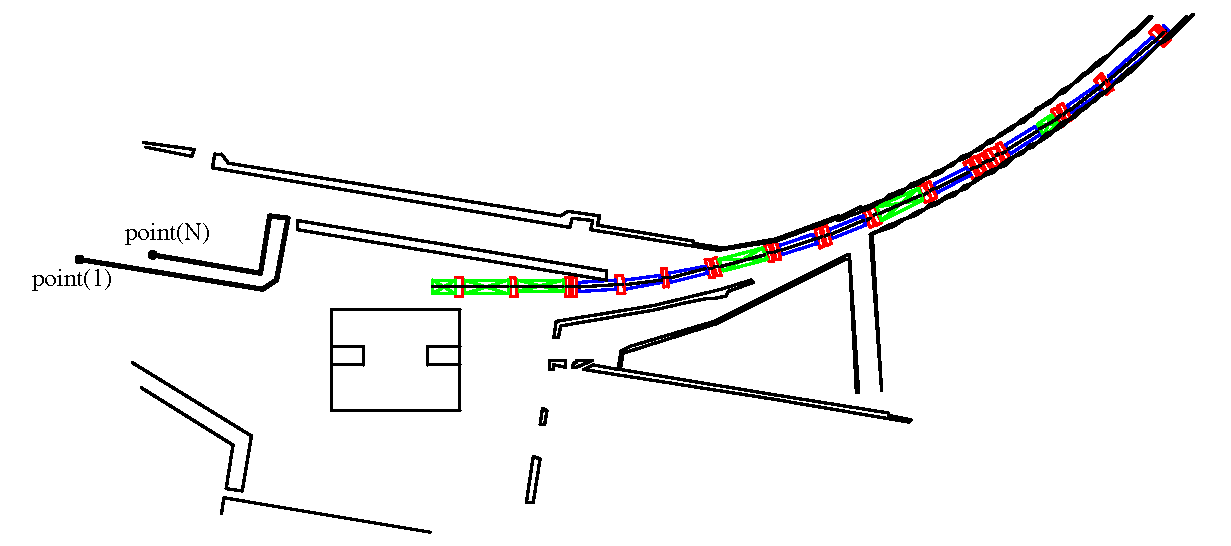
\includegraphics[width=5in]{building-wall.pdf}
  \caption[Floor_plan drawing showing the walls of the building]
{Floor_plan drawing showing the walls of the building (along with a section of a recirculation
arc). Defining building walls can be useful for such things as floor plots and designing a machine
to fit in an existing building.}
  \label{f:building.wall}
\end{figure}

A two dimensional cross-section of the building containing the machine under simulation may be defined in
\tao. This can be useful when drawing \vn{floor_plan} plots of the machine (\sref{s:floor.plan}) or
to design a machine to fit within an existing building by using optimization (\sref{c:opti}).

The wall cross-sections are defined by a set of ``\vn{sections}''. A section is a curve in the
horizontal $Z$-$X$ plane that defines where the face of a wall is. One such section is highlighted in
Figure~\ref{f:building.wall} starting at the point marked ``point(1)'' and ending at the point
marked ``point(N)''. Each section is defined by a set of points which are connected together using
straight lines or circular arcs.

The name of the file containing the building wall definition is given by the \vn{building_wall_file}
variable in the \vn{tao_start} namelist (\sref{s:init.begin}). In general, this file will contain a
number of \vn{building_wall_section} namelists. Each \vn{building_wall_section} namelist defines a
single wall section. The syntax of this namelist is
\begin{example}
  &building_wall_section
    \{name = <string>\}
    \{constraint = <type>\}
    point(1) = <z1>, <x1>
    point(2) = <z2>, <x2>, \{<r2>\}
    point(3) = <z3>, <x3>, \{<r3>\}
    ... etc ...
    point(N) = <zN>, <xN>, \{<rN>\}
  /
\end{example}
The optional \vn{name} component allows for matching wall sections to \vn{floor_plan} shapes
(\sref{s:shapes}) when drawing a \vn{floor_plan} so that different portions of the wall can be drawn
in different colors.

The global coordinate system in \bmad (see the \bmad manual) defines the $(Z, X)$ plane as being
horizontal.  [Note: $(Z, X)$ is used instead of $(X, Z)$ since $(Z, X, Y)$ forms a right handed
coordinate system.] The points that define a wall section are specified in this coordinate system.
In the \vn{building_wall_section} namelist, the $(Z, X)$ position of each point defining a wall
section is given along with an optional radius $r$. If a non-zero radius is given for point $j$,
then the segment between point $j-1$ and $j$ is a circular arc of the given radius. If no radius is
given, or if it is zero, the segment is a straight line. A radius for the first point, number 1,
cannot be specified since this does not make sense. Additionally, a radius must be at least half the
distance between the two points that define the end points of the arc.

In general, given two end points and a radius, there are four possible arcs that can be drawn. The
arc chosen follows the following convention:
\begin{enumerate}
\item
The angle subtended by the arc is 180 degrees or less.
\item
If the radius for the arc from $j-1$ to $j$ is positive, the arc curves in a clockwise manner. If
the radius is negative, the arc curves counterclockwise. This convention mimics the convention used
for \vn{rbend} and \vn{sbend} elements.
\end{enumerate}
To define a wall that is circular, use three points with two 180
degree arcs in between.

When designing a machine to fit within the walls of a building, the \vn{constraint} variable of the
namelist is used to designate whether the given wall section is on the $+x$ (left) side of the
machine or the $-x$ (right) side. Here $x$ is the local reference frame transverse coordinate. See
the write up of the \vn{wall.right_side} and \vn{wall.left_side} constraints in \sref{s:data.types}
for more details. Possible values for \vn{constraint} are:
\begin{example}
  "right_side"  ! Section is to be used with wall.right_side constraints
  "left_side"   ! Section is to be used with wall.left_side constraints
  "none"        ! Default. Section is ignored in any constraint calculation.
\end{example}
Using \vn{"none"} for \vn{constraint} is convenient for drawing building components on a
\vn{floor_plan} that are not used as an optimization constraint.

Example:
\begin{example}
  &building_wall_section
    constraint = "left_side"   
    point(1) =  23.2837,    8.2842
    point(2) = -10.9703,   13.8712,   107.345
    point(3) = -10.8229,   14.7737
  /
\end{example}
In this example, point 1 is at $(Z, X) = (23.2837, 8.2842)$, the segment between points 1 and 2 is
an arc with a radius of 107.345 meters, and the segment between points 2 and 3 is a straight
line. Also this wall section is to be used when evaluating any \vn{wall.x+} constraint.

If the machine varies vertically ($y$-direction), vertical constraints may be imposed using the
\vn{floor.y} data type (\sref{s:data.types}).

To see a list of the building wall points when running \tao, use the \vn{show building_wall}
(\sref{s:show.building}) command .

Note: To position a machine in the global coordinate system, the starting point and starting
orientation can be adjusted using \vn{beginning[...]} statements as explained in the \bmad manual.

%-----------------------------------------------------------------
\subsection{Building Orientation}
\label{s:building.orient}

It may be convenient to use a different two-dimensional coordinate system for the horizontal plane
than the global coordinate system used by \bmad and \tao. For example, if the building wall coordinates are
obtained from a blueprint. To help with this, an overall position and angle
shift may be specified by a \vn{building_wall_orientation} namelist in the same file with the
\vn{building_wall_section} namelists. The syntax of the \vn{building_wall_orientation} namelist is:
\begin{example}
  theta = <Real>      ! Angle rotation in radians. Default is 0.
  z_offset = <Real>   ! Z-offset. Default is 0.
  x_offset = <Real>   ! X-offset. Default is 0.
\end{example}
The transformation from the input coordinates of a wall point specified in a \vn{build_wall_section} namelist
to the global coordinate system is
\begin{equation}
  \begin{pmatrix} z \\ x \end{pmatrix}_{global} = 
  \begin{pmatrix} \text{z_offset} \\ \text{x_offset} \end{pmatrix} +
  \begin{pmatrix} \cos(\text{theta}) & -\sin(\text{theta}) \\
                   \sin(\text{theta}) & \cos(\text{theta}) \end{pmatrix} \,
  \begin{pmatrix} z \\ x \end{pmatrix}_{input} 
\end{equation}

%-----------------------------------------------------------------
\section{Dynamic Aperture Calculation Initialization}
\index{dynamic aperture}
\label{s:da.calc}

\begin{figure}
  \centering
  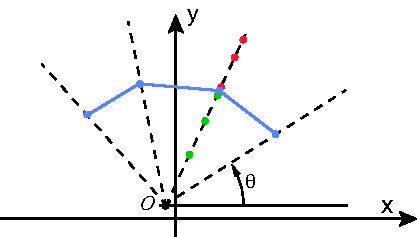
\includegraphics[width=5in]{dynamic-aperture-rays.pdf}
  \caption[Dynamic aperture plot.]{
The calculation of a dynamic aperture curve in the $x$-$y$ plane at a given initial $p_z$ value
involves calculating aperture curve points (blue dots) along a set of ``rays'' (dashed lines) having
a common origin point ($\cal O$) which is taken to be the reference orbit. The line segments between
points is simply for visualization purposes. The calculation of an aperture curve point along a
given ray involves iteratively tracking particles with different starting $(x, y)$ position values
to find the boundary between stable (green dots) and unstable (red dots) motion.
  }
  \label{f:da-rays}
\end{figure}

For historical reasons, the \vn{dynamic_aperture} program (another Bmad based program included in
Bmad Distributions) is also capable of calculating the dynamic aperture.  In fact both programs use
the same underlying code for the aperture analysis. The basic difference is that the
\vn{dynamic_aperture} program is more flexible in terms of tracking. For example, the
\vn{dynamic_aperture} program can handle \vn{ramper} elements and track with maps.

In a storage ring, the ``\vn{dynamic aperture}'' is the region in phase space within which a
particle will stably oscillate. That is, the region within which the motion is bounded. This is in
contrast to the ``\vn{physical aperture}'' which is defined by the vacuum chamber walls. Since it
may take many turns for particle motion to become unstable, calculating the stability region for the
full six-dimensional phase space is a time intensive process.  In light of this, \tao uses a
simplified calculation as discussed below.

In \tao, the motion of a particle is taken to be ``stable'' if the particle survives (does not hit
the physical aperture or does not diverge to large amplitude) in tracking over some set number of
turns.\footnote
  {
If the dynamic aperture is larger than the physical aperture the calculated boundary curve will
reflect the physical aperture and not the dynamic aperture. In practice, this possible confusion is
not a concern since if the dynamic aperture is outside the physical aperture there is no worry that
the dynamic aperture will limit machine performance.
  }
 A typical number is 1000 turns. A dynamic aperture ``scan'' is the calculation of the dynamic
aperture in $(x, y)$ space at some given initial phase space $p_z$ as illustrated in
\fig{f:da-plot}. An $(x, y)$ point represents the initial $x$ and $y$ phase space position of
the particle with the initial $p_x$, $p_y$, and $z$ values being set equal to the closed orbit
values. To calculate an aperture curve for a given initial $p_z$, a set of ``rays" (dashed lines in
the figure) are constructed. The rays have a common origin point ($\cal O$) which is the closed
orbit $(x, y)$ point. On each ray, the boundary point between stable and unstable motion (blue
points in the figure) is found by iteratively tracking particles with initial $(x, y)$ points on the
ray (red and green dots) until the boundary point is determined with the specified accuracy.

The origin point of the rays is taken to be the closed orbit at the given $p_z$ and RF off. This is
true even if the RF is on for the tracking. The reason for this is that with the RF on, there is no
well defined closed orbit at constant $p_z$ (since $p_z$ is not a constant of the motion with the RF
on).

Having the RF off when tracking suppresses synchrotron oscillation effects which may be
important. It is therefore recommended to have the RF on unless there is a good reason for ignoring
synchrotron oscillations. It is also recommended that the lattice element at which the tracking
begins be in a zero dispersion region.

To calculate the dynamic aperture for the $i$\Th universe, the \vn{design(N)%dynamic_aperture_calc}
parameter must be set True in the \vn{tao_design_lattice} namelist (\sref{s:init.lat}). Example:
\begin{example}
  &tao_design_lattice
    design_lattice(1)%file = "lat.bmad"
    design_lattice(1)%dynamic_aperture_calc = T
  /
\end{example}
Alternatively, the aperture calculation can be turned on during running using the \vn{set} command
(\sref{s:set.universe}):
\begin{example}
  set universe 1 dynamic_aperture_calc on
\end{example}
Since aperture calculations take time, once an aperture calculation is done, the calculation is
turned off so to perform multiple scans within a given session, the \vn{set universe} command must
be repeatedly done.

The \vn{show dynamic_aperture} command (\sref{s:show.da}) shows parameter values and the
\vn{set dynamic_aperture} command (\sref{s:set.da}) can be used to change parameter values.

If Tao is compiled with \vn{OpenMP} enabled (\sref{s:openmp}), the dynamic aperture calculation will
be done in parallel.

Parameters for the dynamic aperture simulation are set in the \vn{tao_dynamic_aperture} namelist
(\sref{s:init.begin}) in the \tao root initialization file. Multiple \vn{tao_dynamic_aperture}
namelists may be present if different universes need different parameter values. Example:
\begin{example}
  &tao_dynamic_aperture
    ix_universe = -1             ! Universe to apply to. -1 = all universes.
    pz = 0, 0.01, 0.15           ! List of phase space pz to start scans at.
    a_emit = 1e-11               ! A-mode emittance. Used for data calc.
    b_emit = 1e-13               ! B-mode emittance. Used for data calc.
    ellipse_scale = 10           ! Scale for drawing the ellipse in beam sigmas.
    da_param%start_ele = ''      ! Lattice element to start tracking at.
    da_param%n_angle = 21        ! Number of angles in scan of each energy
    da_param%min_angle = 0       ! Starting scan angle (rad).
    da_param%max_angle = 3.1416  ! Ending scan angle (rad).
    da_param%n_turn = 2000       ! Number of turns a particle must survive
    da_param%rel_accuracy = 1e-2 ! Relative accuracy of boundary point.
    da_param%abs_accuracy = 1e-5 ! Absolute accuracy of boundary point (meters).
    da_param%x_init = 1e-3       ! Initial horizontal aperture estimate. Default: 1e-3 meters.
    da_param%y_init = 1e-3       ! Initial vertical aperture estimate. Default: 1e-3 meters.
  /
\end{example}
Parameters:
\begin{description}
\item[ellipse_scale] \Newline
Scale for drawing the beam ellipse. The default value is 1 which will result in an ellipse drawn
at 1 sigma.
%
\item[ix_universe] \Newline
The \vn{ix_universe} parameter set which universe the parameters are applied to. Any universe index
below a value of one results in the parameter values being applied to all universes.
%
\item[pz] \Newline
The \vn{pz} parameter array is a list of $p_z$ values to use. The number of scans (dynamic aperture curves)
that are produced is equal to the number of \vn{pz} values.
%
\item[a_emit, b_emit] \Newline
Emittance values for the $a$ (``horizontal like'') and $b$ (``vertical like'') normal modes. The
emittance values do not affect particle tracking but are used to draw the beam sigma ellipse in
dynamic aperture plots (\sref{s:da.plot}) and to calculate the \vn{dynamic_aperture.$N$} datum values
(\sref{s:data.types}). 
%
\item[da_param\%start_ele] \Newline
This parameter sets the starting element for tracking. If not set, the beginning element of the
root branch is used. \vn{da_param%start_ele} may be set to either the element name or element index.
%
\item[da_param\%n_angle] \Newline
The number of boundary points calculated for a scan is set by the \vn{da_param%n_angle} parameter. 
%
\item[da_param\%min_angle, da_param\%max_angle] \Newline
These parameters set the ray minimum and maximum angles, labeled $\theta$ in \fig{f:da-plot}, in a
scan. In the example above the angle ranges from 0 to $pi$.  That is, the upper half-plane. These
are typical settings since typically storage rings are vertically symmetric so the aperture curves
should vertically symmetric as well.

The angles between adjacent rays is not uniform but are rather calculated to give a roughly
equal spacing between boundary points. This is done by looking at the aperture
points on a horizontal and a vertical ray and then scaling the ray angles appropriately).
%
\item[da_param\%rel_accuracy, da_param\%abs_accuracy] \Newline
These parameters set the relative and absolute accuracies that determine when the search for a
boundary point is considered accurate enough.

If $r = \sqrt{(x-x_0)^2 + (y-y_0)^2}$ is the distance
along any ray of the computed boundary point, where $(x_0, y_0)$ are the coordinates of the origin
point, the search for the boundary point will stop then the accuracy of the boundary point is below
the desired accuracy $\sigma_{cut}$ which is computed from
\begin{equation}
  \sigma_{cut} = \sigma_a + r \, \sigma_r
\end{equation}
with $\sigma_a$ begin the absolute accuracy and $\sigma_r$ being the relative accuracy.
%
\item[da_param\%x_init, da_param\%y_init] \Newline
These parameters set the initial $x$ and $y$ values used in the first two boundary point searches.
The values of these parameters will not affect significantly affect the computed curve but will
affect the computation time. If not set, these parameters will default to 0.001 meter.
\end{description}

To plot the results, an appropriate plot must be defined (\sref{s:da.plot}) and \vn{placed} in the
plotting window (\sref{s:init.plot}). An example dynamic aperture plot is shown in
Fig.~\ref{f:da-plot}.

Example input files for calculating and plotting the dynamic aperture are at (\sref{s:examples}):
\begin{example}
  \$ACC_ROOT_DIR/bmad-doc/tao_examples/dynamic_aperture
\end{example}

%-----------------------------------------------------------------
\section{Plotting Initialization}
\index{plotting initializing}
\label{s:init.plot} 

\tao has a graphical display window, called the \vn{plot page} (\sref{s:plot.page.def}) within which
such things as lattice functions, machine layout, beam positions, etc., can be plotted. An example
display is shown in \fig{f:plot.typ}.

Plotting is defined by an initialization file whose name is defined by the \vn{plot_file} component
of the \vn{tao_start} namelist (\sref{s:init.begin}).

%-----------------------------------------------------------------
\subsection{Plot Page and Plot Regions}
\label{s:plot.page}
\index{initialization!plotting!plot window}

The \vn{tao_plot_page} namelist (\sref{s:format}) in the plot initialization file
(\sref{s:init.begin}) sets \vn{plot page} (\sref{s:plot.page.def}) parameters including \vn{region}
definitions and the initial placement of plots. The syntax of this namelist is:
\index{tao_plot_page}\index{plot_page!n_curve_pts}
\index{plot_page!size}\index{plot_page!border}
\index{plot_page!text_height}\index{plot_page!title}
\index{region!name}\index{region!location}\index{place}
\begin{example}
  &tao_plot_page
    plot_page%title                    = "<string>", <x>, <y>, "<units>", "<justify>"
    plot_page%subtitle                 = "<string>", <x>, <y>, "<units>", "<justify>"
    plot_page%plot_display_type        = "<string>"  ! Display type: "X" or "TK"
    plot_page%size                     = <x_size>, <y_size>  ! Window size (POINTS) 
    plot_page%border                   = <qp_rect_struct>    ! Border around edge
    plot_page%text_height              = <real>   ! height in POINTS. Def = 12
    plot_page%main_title_text_scale    = <real>   ! Rel to text_height. Def = 1.3
    plot_page%graph_title_text_scale   = <real>   ! Rel to text_height. Def = 1.1
    plot_page%axis_number_text_scale   = <real>   ! Rel to text_height. Def = 0.9
    plot_page%axis_label_text_scale    = <real>   ! Rel to text_height. Def = 1.0
    plot_page%legend_text_scale        = <real>   ! Rel to text_height. Def = 0.8
    plot_page%key_table_text_scale     = <real>   ! Rel to text_height. Def = 0.9
    plot_page%floor_plan_shape_scale   = <real>   ! Floor_plan shape size scaling.
    plot_page%floor_plan_text_scale    = <real>   ! Floor_plan shape text scaling.
    plot_page%lat_layout_shape_scale   = <real>   ! Lat_layout shape size scaling.
    plot_page%lat_layout_text_scale    = <real>   ! Lat_layout shape text scaling.
    plot_page%n_curve_pts              = <int>    ! Num points used to construct a 
                                                  !   smooth curve. Default = 401
    plot_page%box_plots                = <T/F>    ! For debugging. Default = F.
    plot_page%delete_overlapping_plots = <T/F>    ! Default = T.
    plot_page%draw_graph_title_suffix  = <T/F>    ! Default = T.
    include_default_plots              = <T/F>    ! Include default templates? Def = T.
    region(N) = "<region_name>" <x1>, <x2>, <y1>, <y2>  
    place(N)  = "<region_name>", "<template_name>"
    default_plot%...                            ! See below.
    default_graph%...                           ! See below. 
  /
\end{example}

For example:
\begin{example}
  &tao_plot_page
    plot_page%title = "CESR Lattice", 0.5, 0.996, "%PAGE", "CC"
    plot_page%plot_display_type = "X"        ! X11 window.  "TK" is alternative.
    plot_page%size        = 700, 800         ! Points
    plot_page%border      = 0, 0, 0, 50, "POINTS"  
    plot_page%text_height = 12.0
    region(1) = "top"    0.0, 1.0, 0.5, 1.0
    region(2) = "bottom" 0.0, 1.0, 0.0, 0.5
    place(1)  = "top",    "orbit"
    place(2)  = "bottom", "phase"
    default_graph%x%min = 100
    default_graph%x%max = 200
  /
\end{example}

The \vn{tao_plot_page} namelist has the following parameters:
\begin{description}
%
\item[default_graph] \Newline
The \vn{default_graph} parameter is used to set defaults for any \vn{graph} component
defined in any \vn{tao_template_graph} namelist (\sref{s:template}). Example
\begin{example}
  &tao_plot_page
    default_graph%x%min = 0
    default_graph%x%max = 100
    ...
\end{example}
This sets the default \vn{x}-axis bounds. Also see \vn{default_plot} below.
%
\item[default_plot] \Newline
The \vn{default_plot} parameter is used to set defaults for any \vn{plot} component
defined in any \vn{tao_template_plot} namelist (\sref{s:template}). Example:
\begin{example}
  &tao_plot_page
    default_plot%x_axis_type = "index"
    ...
\end{example}
This sets the default \vn{%x_axis_type}. Also see \vn{default_graph} above.
%
\item[include_default_plots] \Newline
If \vn{include_default_plots} is set to \vn{False}, the collection of template plots
(\sref{s:template}) that \tao constructs by default are not constructed. The default is True.  Note:
If \vn{include_default_plots} is True, and if a user defines a template plot that has the same name
as a default plot, the default plot will not be instantiated.
%
\item[place(N)] \Newline
The \vn{place(N)} parameter, with \vn{N} being an integer, determines the initial placement of
plots (\sref{s:plot.def}).  If no \vn{place} parameters are set, the default \vn{orbit}, \vn{beta},
\vn{dispersion}, and \vn{lat_layout} plots will be displayed. Each \vn{place(N)} has the syntax:
\begin{example}
  &tao_plot_page
    place(N) = "<region_name>" "<plot_template_name>"
    ...
\end{example}
\vn{"<region_name>"} is the region name and \vn{"<plot_template_name>"} is the name of the template
plot to put in the region. Examples:
\begin{example}
  &tao_plot_page
    place(1)  = "top",    "orbit"   ! Orbit plot placed in "top" region
    place(2)  = "bottom", "phase"   ! Phase plot placed in "bottom" region
    ...
\end{example}
%
\item[plot_page\%axis_number_text_scale] \Newline
This along with \vn{plot_page%text_height} sets the font size for the plot page title. See
\vn{plot_page%text_height} for more details.
%
\item[plot_page\%axis_label_text_scale] \Newline
This along with \vn{plot_page%text_height} sets the font size for the plot page title. See
\vn{plot_page%text_height} for more details.
%
\item[plot_page\%border] \Newline
\vn{plot_page%border} sets a border around the edges of the window. As shown in
Figure~\ref{f:plot.page}, the offsets \vn{x1}, \vn{x2} in black (corresponding to \vn{%border%x1}
and \vn{%border%x2}) are the right and left border widths and the offsets \vn{y1} and \vn{y2} in
black (corresponding to \vn{%border%y1} and \vn{%border%y2}) are the bottom and top border widths
respectively. The rectangle within this border is called the \vn{plot area}.
%
\item[plot_page\%curve_legend] \Newline
Sets parameters for the curve legend (\sref{s:plot.def}). \vn{%curve_legend} is an instance of a
\vn{qp_legend_struct} (\sref{s:qp.legend.str}). Note: When drawing a curve legend for a particular
graph, the placement of the legend is given by \vn{graph%curve_legend_origin}.
%
\item[plot_page\%delete_overlapping_plots] \Newline
When \vn{plot_page%delete_overlapping_plots} is True (the default), Placing a plot (using
the \vn{place} command \sref{s:place}) causes any existing plots that overlap the
placed plot to become invisible. 
%
\item[plot_page\%draw_graph_title_suffix] \Newline
The \vn{plot_page%draw_graph_title_suffix} is used to suppress the drawing of the string that
is printed to the right of a graph title (set by \vn{graph%title}). This string is set by \tao
and has information on what is being plotted (typically the \vn{curve%component}). To suppress
the suffix, set \vn{plot_page%draw_graph_title_suffix} to False.
%
\item[plot_page\%floor_plan_shape_scale] \Newline
This parameter sets the overall scale for drawing shapes for a \vn{floor_plan} drawing
(\sref{s:shapes}). The default value is 1.
%
\item[plot_page\%floor_plan_text_scale] \Newline
Sets the font size of \vn{floor_plan} shape labels. The font size is the product
\begin{example}
  size = plot_page%text_scale * plot_page%legend_text_scale * plot_page%floor_plan_text_scale
\end{example}
%
\item[plot_page\%graph_title_text_scale] \Newline
This along with \vn{plot_page%text_height} sets the font size for the plot page title. See
\vn{plot_page%text_height} for more details.
%
\item[plot_page\%key_table_text_scale] \Newline
This along with \vn{plot_page%text_height} sets the font size for the plot page title. See
\vn{plot_page%text_height} for more details.
%
\item[plot_page\%lat_layout_shape_scale] \Newline
This parameter sets the overall scale for drawing shapes for a \vn{lat_layout} drawing
(\sref{s:shapes}). The default value is 1.
%
\item[plot_page\%lat_layout_text_scale] \Newline
Sets the font size of \vn{lat_layout} shape labels. The font size is the product
\begin{example}
  size = plot_page%text_scale * plot_page%legend_text_scale * plot_page%lat_layout_text_scale
\end{example}
%
\item[plot_page\%legend_text_scale] \Newline
Sets the font size of the graph curve legend (\sref{s:curve.legend} relative to
\vn{plot_page%text_height}. See \vn{plot_page%text_height} for more details.
The setting of \vn{plot_page%legend_text_scale} also affects the size of \vn{lat_layout}
and \vn{floor_plan} plots.
%
\item[plot_page\%main_title_text_scale] \Newline
Sets the font size of the the plot page title relative to the \vn{plot_page%text_height}. See
\vn{plot_page%text_height} for more details.
%
\item[plot_page\%n_curve_pts] \Newline
The \vn{plot_page%n_curve_pts} parameter sets the default number of points to use for drawing
``smooth'' curves. The default is 401. This default may be overridden for individual plots by
setting the \vn{plot%n_curve_pts} component of a plot (\sref{s:template}). If \vn{plot%n_curve_pts}
is set for an individual plot, that value overrides the value of
\vn{plot_page%n_curve_pts}. Warning: \tao will cache intermediate calculations used to compute a
smooth curve to use in the computation of other smooth curves. \tao will only do this for curves
that have \vn{plot_page%n_curve_pts} number of points. Depending upon the circumstances, setting
\vn{plot%n_curve_pts} for individual plots may slow down plotting calculations significantly.
%
\item[plot_page\%plot_display_type] \Newline
The \vn{plot_page%plot_display_type} component sets the type of plot display
window used. possibilities are:
\begin{example}
  "X"      X11 window
  "TK"     tk window
  "QT"     Available only when using PLPLOT (and not PGPLOT)
\end{example}
Note: The environment variable \vn{ACC_PLOT_DISPLAY_TYPE} sets the default display type. You can
set this variable in your login file to avoid having to setup a \tao init file to set this.
%
\item[plot_page\%size] \Newline
The \vn{plot_page%size} parameter sets the horizontal and vertical size of the plot window in
\vn{points} (\sref{s:qp.units}). Also then environmental variable \vn{ACC_DPI_RESOLUTION}
(\sref{s:plot.page.def}) can be used to vary the window size.
%
\item[plot_page\%subtitle] \Newline
Subtitle text of the plot. See the description for \vn{plot_page%title}. The defaults here are the
same as \vn{plot_page%title} except that \vn{y} defaults to 0.97.
%
\item[plot_page\%text_height] \Newline
The \vn{plot_page%text_height} parameter sets the overall height of the text that is
drawn. Relative to this, various parameters can be used to scale
individual types of text:
\begin{example}
  &tao_plot_page
    plot_page%main_title_text_scale  = 1.3 ! Main title height. 
    plot_page%graph_title_text_scale = 1.1 ! Graph title height.
    plot_page%axis_number_text_scale = 0.9 ! Axis number height
    plot_page%axis_label_text_scale  = 1.0 ! Axis label height.
    plot_page%key_table_text_scale   = 0.8 ! Key Table text (\sref{s:key.table}).
    plot_page%legend_text_scale      = 0.9 ! Lat Layout or floor plan text.
    ...
\end{example}
The default values for these scales are given above.
%
\item[plot_page\%title] \Newline
The \vn{plot_page%title} sets the page title which is text that is generally printed at the top of
the page.  This parameter is a structure which has components:
\begin{example}
  string = ""         ! Text to print
  x = 0.50            ! Horizontal position
  y = 0.99            ! Vertical position
  units = "%PAGE"     ! Units of x and y (\sref{s:qp.units})
  justify = "CC"      ! Justification (\sref{s:qp.str.just})
\end{example}
The values shown are the defaults.
Also see \vn{page%subtitle}.
%
\item[region(N)] \Newline
The \vn{region(N)} parameter, with \vn{N} being an integer, is used to create custom regions
(\sref{s:region.def}) in addition to the default regions defined by \tao. 
Each \vn{region(N)} has the syntax:
\begin{example}
    region(N) = "<region_name>" <x1>, <x2>, <y1>, <y2>  
\end{example}
\vn{"<region_name>"} is the region name which may not contain a dot ``.'' or a space.  The other
four elements \vn{<x1>}, \vn{<x2>}, \vn{<y1>}, and \vn{<y2>} define the region position on the plot
page as discussed in \Sref{s:region.def}. There is no upper limit to the number of regions that can
be defined.
\begin{example}
  &tao_plot_page
    region(1) = "top"    0.0, 1.0, 0.5, 1.0
    region(2) = "bottom" 0.0, 1.0, 0.0, 0.5
    ...
\end{example}
%
\end{description}

%-----------------------------------------------------------------
\subsection{Plot Templates}
\label{s:template}
\index{plot templates}

A plot \vn{template} (\sref{s:plot.def}) defines a set of parameters used for constructing a
\vn{displayed} plot. \tao, by default, defines a number of template plots. User defined template
plots are constructed with a \vn{tao_template_plot} namelist in the plot initialization file
(\sref{s:init.begin}) along with zero or more \vn{tao_template_graph} namelists, one for each
\vn{graph} associated with the template plot. The syntax for the \vn{tao_template_plot} is:
\index{tao_template_plot}
\index{plot!name}
\index{plot!x}
\index{plot!x_axis_type}
\index{plot!n_graph}
\index{plot!autoscale_gang_x}
\index{plot!autoscale_gang_y}
\index{plot!autoscale_x}
\index{plot!autoscale_y}
\begin{example}
  &tao_template_plot
    plot%name        = "<plot_name>"
    plot%x_axis_type = "<x_axis_type>"   ! "index", "ele_index" "s", "lat", "var", etc. 
    plot%autoscale_gang_x = <logical>    ! Default: True.
    plot%autoscale_gang_y = <logical>    ! Default: True.
    plot%autoscale_x = <logical>         ! Default: False.
    plot%autoscale_y = <logical>         ! Default: False.
    plot%n_curve_pts = <integer>         ! Used to override plot_page%n_curve_pts.
    plot%n_graph     = <n_graphs>
    default_graph%...                    ! See below
    default_curve%...                    ! See below
  /
\end{example}
For example:
\begin{example}
  &tao_template_plot
    plot%name                         = "orbit"
    default_graph%x%major_div_nominal = 10
    default_graph%x%label             = "Index"
    default_graph%y%max               = 10
    plot%n_graph                      = 2
  /
\end{example}

The \vn{tao_plot_page} namelist has the following parameters:
\begin{description}
%
\item[default_curve] \Newline
The \vn{default_curve} sets defaults for \vn{curves} associated with the plot. 
The \vn{default_curve} is a structure with the same components
as the \vn{curve} parameter of the \vn{tao_template_graph} structure discussed below.
%
\item[default_graph] \Newline
The \vn{default_graph} sets defaults for \vn{graphs} associated with the plot. This is useful if
there are multiple associated graphs. The \vn{default_graph} is a structure with the same components
as the \vn{graph} parameter of the \vn{tao_template_graph} structure discussed below.

Settings of \vn{default_graph} in the \vn{tao_template_plot} namelist overrides, for the graphs
associated with the plot, any \vn{default_graph} settings made in the \vn{tao_template_plot}
namelist (\sref{s:init.plot}).
%
\item[plot\%autoscale_gang_x] \Newline
The \vn{plot%autoscale_gang_x} parameter is relavent if the plot has more than one associated
graph. In this case, if set to True (the default), and if the \vn{x_scale} command
(\sref{s:x.scale}) is applied to the plot (as opposed to being applied to an individual graph),
the data of all the graphs is combined to compute a horizontal scale which is used for all the graphs.
If \vn{%autoscale_gang_x} is set to False, graphs are scaled individually.
%
\item[plot\%autoscale_gang_y] \Newline
The \vn{plot%autoscale_gang_y} parameter is relavent if the plot has more than one associated
graph. In this case, if set to True (the default), and if the \vn{scale} command
(\sref{s:scale}) is applied to the plot (as opposed to being applied to an individual graph),
the data of all the graphs is combined to compute a vertical scale which is used for all the graphs.
If \vn{%autoscale_gang_y} is set to False, graphs are scaled individually.
%
\item[plot\%autoscale_x] \Newline
Plots with \vn{plot%autoscale_x} set to True will
automatically rescale the horizontal axis after any calculation. Default is False.
%
\item[plot\%autoscale_y] \Newline
Plots with \vn{plot%autoscale_y} set to True will
automatically rescale the vertical axes after any calculation. Default is False.
%
\item[plot\%n_curve_pts] \Newline
The \vn{plot%n_curve_pts} parameter sets the number of evaluation points to use for drawing
``smooth'' curves (\sref{s:curve.def}). This overrides the setting of \vn{plot_page%n_curve_pts}
(\sref{s:init.plot}). Warning: \tao will cache intermediate calculations used to compute a smooth
curve to use in the computation of other smooth curves. \tao will only do this for curves that have
\vn{plot_page%n_curve_pts} number of points. Depending upon the circumstances, setting
\vn{plot%n_curve_pts} for individual plots may slow down plotting calculations significantly.
%
\item[plot\%n_graph] \Newline
The \vn{plot%n_graph} parameter sets the number of graphs associated with the plot and each one
needs a \vn{tao_template_graph} namelist to define it. These namelists should be placed directly
after their respective \vn{tao_template_graph} namelist.
%
\item[plot\%name] \Newline
The \vn{plot%name} parameter is the name that is used with \tao commands to identify the plot
(\sref{s:plot.def}). It is important that this name not contain any blank spaces since \tao uses
this fact in parsing the command line.
%
\item[plot\%x_axis_type] \Newline
The \vn{plot%x_axis_type} parameter sets what is plotted along the \vn{x_axis}. Possibilities are:
\index{index}\index{ele_index}\index{s}
\begin{example}
    "index"         ! Data Index.
    "ele_index"     ! Element lattice number index.
    "s"             ! Longitudinal position in the lattice.
    "s_expression"  ! s-dependent expression involving lattice parameters.
    "data"          ! From a data array.
    "lat"           ! Lattice variable. See \sref{s:plot.var}.
    "var"           ! Tao variable value. See \sref{s:plot.var}.
    "phase_space"   ! Set by \tao if graph%type = "phase_space".
    "none"          ! Set by \tao if graph%type = "key_table".
    "floor"         ! Set by \tao if graph%type = "floor_plan".
\end{example}

The \vn{ele_index} switch is used when plotting data arrays. In this
case the \vn{index} switch refers to the index of the data array and
\vn{ele_index} refers to the index of the lattice element that the
datum was evaluated at.
%
\end{description}

The number of graphs associated with a template plot is specified by the setting of
\vn{plot%n_graph} in the \vn{tao_template_plot} namelist.  For each associated graph there needs to
be a \vn{tao_template_graph} namelist. These namelists need to be placed directly below the
\vn{tao_template_plot} namelist. Each \vn{tao_template_graph} namelist must have a \vn{graph_index}
parameter with the first \vn{tao_template_graph} namelist below the \vn{tao_template_plot} namelist
having \vn{graph_index} set to \vn{1}, the next \vn{tao_template_graph} having \vn{graph_index} set
to \vn{2}, etc.

The general format of the \vn{tao_template_graph} namelist is:
\index{tao_template_graph}\index{graph!y}\index{curve!name}
\index{graph_index}\index{graph}\index{graph!name}\index{curve}
\index{graph!type}\index{graph!box}\index{graph!title}\index{graph!margin}
\index{graph!y2}\index{graph!n_curve}\index{graph!clip}\index{graph!component}
\index{graph!symbol_size_scale}
\index{curve!data_type}\index{curve!data_source}
\index{curve!x_axis_units_factor}\index{curve!y_axis_units_factor}
\index{curve!use_y2}\index{curve!line}\index{curve!ele_ref_name}
\index{curve!draw_line}\index{curve!draw_symbols}\index{curve!ix_universe}
\index{curve!symbol}\index{curve!symbol_every}\index{curve!convert}
\index{curve!ix_bunch}\index{curve!data_type_x}
\begin{example}
  &tao_template_graph
    graph_index              = <integer>          ! Graph index. 1 = first graph, etc.
    graph%name               = "<string>"         ! Default is  "g<n>" <n> = graph_index. 
    graph%type               = "<string>"         ! "data", "floor_plan", etc.
    graph%box                = <ix>, <iy>, <ix_tot>, <iy_tot>
    graph%title              = "<string>"         ! Title above the graph.
    graph%text_legend(n)     = "<string>"         ! Set legend text
    graph%text_legend_origin  = <qp_point_struct> ! Placement of the text legend
    graph%curve_legend_origin = <qp_point_struct> ! Placement of the curve legend
    graph%margin             =  <ix1>, <ix2>, <iy1>, <iy2>, "<Units>"
    graph%scale_margin       =  <ix1>, <ix2>, <iy1>, <iy2>, "<Units>"
    graph%x                  = <qp_axis_struct>   ! Horizontal axis.
    graph%y                  = <qp_axis_struct>   ! Left axis.
    graph%y2                 = <qp_axis_struct>   ! Right axis.
    graph%y2_mirrors_y       = <logical>          ! y2 min/max the same as y-axis? Default = T
    graph%clip               = <logical>          ! Clip curves at boundary? Default = T
    graph%draw_axes          = <logical>          ! Default = T
    graph%draw_grid          = <logical>          ! Default = T
    graph%draw_curve_legend  = <logical>          ! Default = T
    graph%draw_title         = <logical>          ! Default = T
    graph%allow_wrap_around  = <logical>          ! Wrap curves around lattice ends?
    graph%symbol_size_scale  = <real>             ! Phase_space plots symbol scale factor
    graph%ix_universe        = <integer>          ! Default = -1 => Use default universe
    graph%ix_branch          = <integer>          ! Lattice branch index. -1 => Use default branch
    graph%floor_plan         = <floor_plan_struct> ! Floor_plan parameters (\sref{s:floor.plan}).
    graph%draw_only_good_user_data_or_vars        ! Veto data or variables with good_user = F?
                                 = <logical>      !   Default = T.
    graph%x_axis_scale_factor    = <factor>       ! Scale the x-axis by this.
    graph%n_curve                = <integer>      ! Limit number of curves.
    curve(N)%name                = "<string>"     ! Default is "c<i>", <i> = curve num.
    curve(N)%data_type           = "<string>"     ! EG: "orbit.x"
    curve(N)%data_source         = "<string>"     ! Source for the data curve points
    curve(N)%data_type_x         = "<string>"     ! Used with plot%x_axis_type = "data" or "var".
    curve(N)%component           = "<string>"     ! Eg: "model - design". 
    curve(N)%data_index          = "<string>"     ! Index number for data points.
    curve(N)%legend_text         = "<string>"     ! Text for curve legend. 
    curve(N)%y_axis_scale_factor = <factor>       ! Scale the y-axis by this.
    curve(N)%use_y2              = <logical>      ! Use left-axis scale?
    curve(N)%draw_line           = <logical>      ! Connect data with lines?
    curve(N)%draw_symbols        = <logical>      ! Draw data symbols?
    curve(N)%draw_symbol_index   = <logical>      ! Print index number next to the data symbol?
    curve(N)%draw_error_bars     = <logical>      ! Draw error bars with data?
    curve(N)%ix_universe         = <integer>      ! Default = -1 => Use default uni.
    curve(N)%ix_branch           = <integer>      ! Default = -1  => Use default lat branch.
    curve(N)%ix_bunch            = <integer>      ! Bunch index. Default = 0 (all bunches).
    curve(N)%n_turn              = <integer>      ! For phase space multi_turn_orbit.
    curve(N)%line     = <qp_line_struct>          ! Line spec (color, width, etc.)
    curve(N)%symbol   = <qp_symbol_struct>        ! Symbol spec (color size, etc.)
    curve(N)%symbol_every      = <integer>        ! Plot symbol every # datums
    curve(N)%ele_ref_name      = "<string>"       ! Name of reference element.
    curve(N)%smooth_line_calc  = <Logical>        ! Calc data between symbol points? 
    curve(N)%orbit   = <tao_graph_orbit_struct>   ! For E & B field plots
    curve(N)%hist    = <tao_histogram_struct>     ! For histograms
    curve(N)%z_color = <tao_curve_color_struct>   ! For phase space plotting
  /
\end{example}
For example:
\begin{example}
  &tao_template_graph
    graph_index               = 1
    graph%name                = "x"
    graph%type                = "data"
    graph%box                 = 1, 1, 1, 2
    graph%title               = "Horizontal Orbit (mm)"
    graph%margin              =  60, 200, 30, 30, "POINTS"
    graph%y%label             = "X"
    graph%y%major_div_nominal = 4
    curve(1)%component        = "model - design"
    curve(1)%data_source      = "data"
    curve(1)%data_type        = "orbit.x"
    curve(1)%units_factor     = 1000
    curve(1)%use_y2           = F
  /
\end{example}

The \vn{tao_template_graph} namelist has the following parameters:
\begin{description}
%
\item[curve(N)\%component] \Newline
The \vn{%component} sets from where data is derived from (\sref{s:curve.comp}).
%
\item[curve(N)\%data_index] \Newline
When used with graphing a data slice (\sref{s:graph.data.slice}), the \vn{%data_index}
parameter sets the index number for the symbol points. The symbol index number can then be displayed
next to the symbol.

When used with graphing the dynamic aperture (\sref{s:da.plot}), the \vn{%data_index} parameter
is used to associate a curve with a given dynamic aperture scan.
%
\item[curve(N)\%data_source] \Newline
The \vn{%data_source} parameter sets where information is drawn in computing curve points
(\sref{s:curve.source}). Used in conjunction with \vn{%data_type} and \vn{%component}. 
%
\item[curve(N)\%data_type] \Newline
The \vn{%data_type} parameter sets what is being computed (\sref{s:curve.type}). Used in
conjunction with \vn{%data_type} and \vn{%component}.
%
\item[curve(N)\%data_type_x] \Newline
Used with data slices (\sref{s:graph.data.slice}).
%
\item[curve(N)\%draw_error_bars] \Newline
The \vn{%draw_error_bars} logical determines whether error bars are drawn when plotting data
(\vn{%data_source} set to \vn{data}). The half height of the error bars is determined by the
\vn{error_rms} values of the data associated with the curve (\sref{s:data.anatomy}).  To keep things
simple, \tao ignores the setting of \vn{%component} when drawing error bars. This must be kept
in mind since for example, the measurement error associated with a difference plot of measured data
minus reference data (when \vn{%component} is set to \vn{meas-ref}) is different from just plotting
measured data, which in turn is different from a plot of the data as calculated from the \vn{model}
(the measurement error associated with this is zero).
%
\item[curve(N)\%draw_line] \Newline
Used to toggle drawing of the curved line associated with a curve (\sref{s:curve.line}). Default is True.
%
\item[curve(N)\%draw_symbol_index] \Newline
Used to toggle drawing of the symbol index. Default is False.
%
\item[curve(N)\%draw_symbols] \Newline
Used to toggle drawing of symbols. Default is True.
%
\item[curve(N)\%ele_ref_name] \Newline
The \vn{%ele_ref_name} component is only used if \vn{%data_source} is set to \vn{"lat"}.
If \vn{%ele_ref_name} is set, the curve will be shifted by subtracting the value of the
parameter being plotted evaluated at the reference element. For example, if \vn{orbit.x} is being
plotted, and \vn{%ele_ref_name} is set to "\vn{Q10W}", the plotted curve will be shifted by
subtracting the value of the horizontal orbit at Q10W. Notice that the shifting is done for each
curve component. For example, if \vn{%component} is set to "\vn{model - design}", the curve
will be shifted by subtracting the difference between the \vn{model} and \vn{design} values
evaluated at the reference element.
%
\item[curve(N)\%hist] \Newline
The \vn{%hist} parameter is a structure used for setting histogram parameters (\sref{s:histogram}).
%
\item[curve(N)\%ix_branch] \Newline
The \vn{%ix_branch} sets which lattice branch data (beta function, orbit, etc.) is taken.
from. Default is -1 which translates to the default branch \vn{global%default_branch}.
%
\item[curve(N)\%ix_bunch] \Newline
The \vn{%ix_bunch} parameter sets which particle bunch data is taken from if \vn{%data_source}
(\sref{s:curve.source}) is set to \vn{"beam"}. Default is 1.
%
\item[curve(N)\%ix_universe] \Newline
The \vn{%ix_universe} parameter sets which universe (\sref{s:universe}) data is taken from. Default
is -1 which means that the data will be drawn from the current default universe \vn{global%default_uni}.
%
\item[curve(N)\%legend_text] \Newline
The \vn{%legend_text} parameter sets the text that is displayed in the curve legend
(\sref{s:curve.legend}) for the curve.
%
\item[curve(N)\%line] \Newline
The \vn{%line} parameter sets parameters associated with curved line associated with the curve
(\sref{s:curve.line}).  This parameter is a structure of type \vn{qp_line_struct}
(\sref{s:qp.line}).
%
\item[curve(N)\%name] \Newline
The identifying name of the curve (\sref{s:curve.name}). Used in \tao commands that manipulate curves.
%
\item[curve(N)\%orbit] \Newline
The \vn{%orbit} parameter, used when plotting electric and magnetic fields, defines the orbit with
constant transverse offset along which the fields are evaluated. This parameter is used when the
\vn{%data_type} is one of the following:
\begin{example}
  b0_field.x,  b0_field.y,  b0_field.z,  b0_curl.x,  b0_curl.y,  b0_curl.z,  b0_div
  e0_field.x,  e0_field.y,  e0_field.z,  e0_curl.x,  e0_curl.y,  e0_curl.z,  e0_div
\end{example}
Note: The data types with names starting with ``b_'' and ``e_'' evaluate the field along the single
particle trajectory.

The \vn{%orbit} is a structure with the following subcomponents:
\begin{example}
  x         ! horizontal $x$-position of orbit.
  y         ! vertical $y$-position of orbit.
  t         ! time to evaluate fields at.
\end{example}
%
\item[curve(N)\%smooth_line_calc] \Newline
Sets if additional points are used to evaluate the curve at so that the drawn line has a ``smooth''
appearance (\sref{s:curve.line}). Default is True.
%
\item[curve(N)\%symbol] \Newline
The \vn{%symbol} parameter sets parameters associated with the symbols to be drawn
(\sref{s:curve.sym}). This parameter is a structure of type \vn{qp_symbol_struct} (\sref{s:qp.sym}).
%
\item[curve(N)\%symbol_every] \Newline
When drawing a set of symbols of a curve, if the density of symbols is too large so that the drawing
is too crowded, The number can be reduced by a factor equal to the value of \vn{%symbol_every}. For
example, a setting of \vn{3} will result in every third symbol being drawn. This is especially
helpful in phase space plots. The default is \vn{1}.
%
\item[curve(N)\%use_y2] \Newline
Use the \vn{y2} axis (\sref{s:axes}) for the curve? Default is False.
%
\item[curve(N)\%y_axis_scale_factor] \Newline
Curve vertical \vn{y} and \vn{y2} axes scale factor. For a given ``datum'' value, the plotted value will be:
\begin{example}
  y(plotted) = scale_factor * y(datum)
\end{example}
The default value is \vn{1}. For example, a \vn{%y_axis_scale_factor} of 1000 will draw a 1.0~mm orbit at the
1.0 mark on the vertical scale. That is, the vertical scale will be in millimeters.
\vn{graph%x_axis_scale_factor}.
%
\item[curve(N)\%z_color] \Newline
The \vn{%z_color} parameter is a structure used for setting false color parameters for phase space
plotting. See \Sref{s:phase.space} for more details.
%
\item[graph\%allow_wrap_around] \Newline
If \vn{plot%x_axis_type} is set to \vn{"s"}, and if the plotted data is from a lattice branch with a
closed geometry, and if \vn{graph%x%min} is negative, then the \vn{graph%allow_wrap_around}
parameter sets if the curves contained in the graph are ``wrapped around'' the beginning of the
lattice so that the curves are not cut off at $s = 0$. The default is \vn{True}.
%
\item[graph\%box] \Newline
The \vn{graph%box} parameter sets the layout of the box which the \vn{graph} is placed in
\sref{s:box.def}. In the above example, the graph divides the \vn{region} the plot is placed in into
two vertically stacked rectangles and the graph will be placed into the bottom one. The default
is \vn{1,1,1,1} which scales a graph to cover the entire \vn{region} the plot is placed in.
%
\item[graph\%clip] \Newline
Clip the graph curves at the graph top and bottom boundaries? Default is \vn{True}.
%
\item[graph\%curve_legend_origin]\Newline
The curve legend displays which curves are associated with which of the plotted lines and symbols. Two
examples are given \fig{f:plot.typ}. The \vn{%curve_legend_origin} defines where the upper left hand
corner of the legend is. The default is:
\begin{example}
  graph%curve_legend_origin%x =  5.0
  graph%curve_legend_origin%y = -2.0
  graph%curve_legend_origin%units = "POINTS/GRAPH/LT"
\end{example}
The \vn{%curve_legend_origin} is of type \vn{qp_point_struct}. See \sref{s:qp.point} for details on this
structure. Also see \vn{graph%draw_curve_legend} and \vn{plot_page%curve_legend}.
%
\item[graph\%draw_axes] \Newline
Draw the graph axes? Default is \vn{True}. 
%
\item[graph\%draw_curve_legend] \Newline
Draw the curve legend? Default is \vn{True}. The curve legend displays which curves are associated
with which of the plotted lines and symbols. Two examples are given \fig{f:plot.typ}. Also see
\vn{graph%curve_legend_origin}.
%
\item[graph\%draw_grid] \Newline
Draw the graph grid? Default is \vn{True}.
%
\item[graph\%draw_only_good_user_data_or_vars] \Newline
When plotting \tao data (\sref{c:data}) or variables (\sref{c:var}): If
\vn{%draw_only_good_user_data_or_vars} is set to True (the default), symbol points of curves in the
graph associated with data or variables whose \vn{good_user} parameter is set to \vn{False} will be
ignored. That is, data and variables that will not be used in an optimization will be ignored. If
\vn{%draw_only_good_user_data_or_vars} is set to False, data or variables that have a valid value
will be plotted.
%
\item[graph\%draw_title] \Newline
Draw the graph title? Default is True.
%
\item[graph\%floor_plan] \Newline
This parameter is a structure whose components are used when drawing a \vn{floor_plan}. See
\Sref{s:floor.plan} for more details.
%
\item[graph\%ix_branch] \Newline
The \vn{graph%ix_branch} parameter sets the default branch for curves of the graph. The default will
be overridden by \vn{curve(N)%ix_branch}. 
%
\item[graph\%ix_universe] \Newline
The \vn{graph%ix_universe} parameter sets the default universe for curves of the graph.
%
\item[graph\%margin] \Newline
\vn{graph%margin} sets the margin between the \vn{graph} and the \vn{box}
it is drawn in.
%
\item[graph\%n_curve] \Newline
If not present, \tao will count the number of curves associated with a graph based on if
\vn{curve(N)%data_type} is set. In the case where \vn{default_curve%data_type} in the
\vn{tao_template_plot} namelist is set, the \vn{graph%n_curve} parameter can be set to
limit the number of curves created.
%
\item[graph\%name] \Newline
\vn{graph%name} and \vn{curve%name} define names to be used with commands. The default names are
just the letter \vn{g} or \vn{c} with the index of the graph or curve. Thus, in the example above,
the name of the curve defaults to \vn{c1} and it would be referred to as \vn{orbit.x.c1}.  It is
important that these names do not contain any blank spaces since \tao uses this fact in parsing the
command line.
%
\item[graph\%scale_margin] \Newline
\vn{graph%scale_margin} is used to set the minimum space between what is being drawn and the edges
of the \vn{graph} when a \vn{scale}, \vn{x_scale}, or a \vn{xy_scale} command is issued. Normally
this is zero but is useful for \vn{floor plan} drawings.
%
\item[graph\%symbol_size_scale] \Newline
%
\item[graph\%text_legend]\Newline
%
\item[graph\%text_legend_origin]\Newline
%
\item[graph\%title] \Newline
The \vn{graph%title} component is the string printed just above the graph box. The full string will also
include information about what is being plotted and the horizontal axis type. To fully suppress the
title leave it blank. Note: A graph also has a \vn{graph%title_suffix} which \tao uses to hold the
string which is printed to the right of the \vn{graph%title}. This string contains information like
what \vn{curve%component} is being plotted. The \vn{graph%title_suffix} cannot be set by the user.
%
\item[graph\%type] \Newline
\vn{graph%type} is the type of graph. \tao knows about the
following types:
\index{data}\index{lat_layout}\index{key_table}\index{phase_space}
\index{floor_plan}\index{beam_chamber_wall}
\begin{example}
  "data"               ! Lattice parameters, data and/or variable plots (default).
  "dynamic_aperture"   ! Dynamic aperture plot (\sref{s:da.plot}).
  "floor_plan"         ! A 2-dimensional birds-eye view of the machine (\sref{s:floor.plan}).
  "histogram"          ! Histogram of plot (\sref{s:histogram}).
  "key_table"          ! Key binding table for single mode (\sref{s:key.table}).
  "lat_layout"         ! Schematic showing placement of the lattice elements (\sref{s:lat.layout}).
  "phase_space"        ! Phase space plots (\sref{s:phase.space}).
\end{example}

With \vn{graph%type} set to \vn{"data"} (\sref{s:graph.types}), data such as orbits and/or variable
values such as quadrupole strengths are plotted. Here ``data'' can be data from a defined data
structure (\sref{c:data}) or computed directly from the lattice, beam tracking, etc. A \vn{"data"}
graph type will contain a number of \vn{curves} and multiple data and variable curves can be drawn
in one graph.

With \vn{graph%type} set to \vn{floor_plan} (\sref{s:floor.plan}), the two dimensional layout of the
machine is drawn.

With \vn{graph%type} set to \vn{histogram} (\sref{s:histogram}), such things such as beam densities
can be histogrammed.

With \vn{graph%type} set to \vn{"key_table"} (\sref{s:key.table}), the key bindings for use in
single mode (\sref{s:key.bind}) are displayed.  Note: The \vn{"key_table"} graph type does not have
any associated \vn{curve}s.

With \vn{graph%type} set to \vn{lat_layout} (\sref{s:lat.layout}), the elements of the lattice are
symbolical drawn in a one dimensional line as a function of the longitudinal distance along the
machine centerline.

With \vn{graph%type} set to \vn{phase_space} (\sref{s:phase.space}), phase space plots are produced.
%
\item[graph\%x] \Newline
The \vn{%x} parameter sets parameters for the \vn{x}-axis (\sref{s:axes}). This parameter is a
structure of type \vn{qp_axis_struct}. See \Sref{s:qp.axis} for more details.
%
\item[graph\%x_axis_scale_factor] \Newline
Sets the horizontal \vn{x}-axis scale factor. For a given ``datum'' value, the plotted value will
be:
\begin{example}
  x(plotted) = scale_factor * x(datum)
\end{example}
The default value is \vn{1}. For example, a \vn{%x_axis_scale_factor} of 1000 will draw a 1.0~mm
phase space $z$ value at the 1.0 mark on the horizontal scale. That is, the horizontal scale will be
in millimeters. Also see \vn{curve(N)%y_axis_scale_factor}.
%
\item[graph\%y] \Newline
The \vn{%y} parameter sets parameters for the \vn{y}-axis (\sref{s:axes}). This parameter is a
structure of type \vn{qp_axis_struct}. See \Sref{s:qp.axis} for more details.
%
\item[graph\%y2] \Newline
The \vn{%y2} parameter sets parameters for the \vn{y2}-axis (\sref{s:axes}). This parameter is a
structure of type \vn{qp_axis_struct}. See \Sref{s:qp.axis} for more details.
%
\item[graph_index] \Newline
The first \vn{tao_template_graph} namelist after the associated \vn{tao_template_plot} namelist must
have the \vn{graph_index} component set to \vn{1}. The next must have \vn{graph_index} set to
\vn{2}, etc. \tao uses the \vn{graph_index} component to check for errors.
%
\end{description}

%-----------------------------------------------------------------
\subsection{Lattice Parameter Graphing}\index{plot!lattice functions}
\label{s:graph.lat.fun}

Templates for plotting lattice parameters such as Twiss parameters or the orbit can be defined by setting
the \vn{data_type} of a curve appropriately. Example:
\begin{example}
  &tao_template_plot
    plot%name = "my_orbit"
    plot%x_axis_type = "s"
    plot%n_graph = 1
    default_curve%y_axis_scale_factor = 1000  ! mm
  /

  &tao_template_graph
    graph_index = 1
    graph%name = "g"
    curve(1:2)%data_type = "orbit.x", "orbit.y"
  /
\end{example}
lattice parameter names correspond to data type name  as listed in \Sref{s:data.table}.

If the \vn{plot%x_axis_type} is set to \vn{"index"}, the horizontal axis will be the lattice element
index.

If the \vn{curve(N)%source} parameter is set to \vn{"beam"} (The default is \vn{"lat"}), beam
tracking must be done (\sref{s:beam.init}) to have a visible plot. Additionally, due to the way \tao
does beam tracking, \tao is only able to evaluate the plotted parameter at the boundaries between
lattice elements. This means that \tao is not able to do the ``smooth'' line calculation.

%-----------------------------------------------------------------
\subsection{Data Slice Graphing}\index{plot!data slice}
\label{s:graph.data.slice}

Note: Data slicing is a type of parametric plotting. For parametric plotting using curve data see
section~\sref{s:param.plot}.

The standard data graph, as presented in the previous subsection, plots data from a given
\vn{d1_data} array. It is also possible to graph data that has been ``sliced'' in other ways. For
example, suppose a number of universes have been established, with each universe representing the
same machine but with different steerings powered. If in each universe an \vn{orbit} \vn{d2_data}
structure has been defined, an example of a data slice is the collection of points (x, y) where:
\begin{example}
  (x, y) = (<n>@orbit.x[23], <n>@orbit.y[23]),  <n> = 1, ..., n_universe
\end{example}
When defining a template for graphing a data slice, the \vn{plot%x_axis_type} is set to \vn{"data"}, and
the \vn{graph%type} must be set to \vn{"data"}, the \vn{curve(:)%data_source} must be set to
\vn{"data"} and the \vn{curve(:)%data_type_x} and \vn{curve%data_type} are used to define the $x$ and
$y$ axes respectively.  In the strings given by \vn{<curve%data_type_x} or \vn{<curve%data_type}, all
substrings that look like \vn{\#ref} are eliminated and the string given by \vn{curve%ele_ref_name}
is substituted in its place.  Similarly, a \vn{\#comp} string is used as a place holder for the
\vn{curve%component} Example:
\begin{example}
  &tao_template_plot
    plot%name = "at_bpm"
    plot%x_axis_type = "data"
    plot%n_graph = 1
  /

  &tao_template_graph
    graph_index = 1
    graph%title = "Orbit at BPM"
    graph%y%label = "y"
    graph%type = "data"
    graph%x_axis_scale_factor = 1000
    graph%x%label = "x"
    curve(1)%component   = "meas - ref"
    curve(1)%data_source = "data"
    curve(1)%data_type_x = "[2:57]@orbit.x[#ref]|#comp"
    curve(1)%data_type   = "[2:57]@orbit.y[#ref]|#comp"
    curve(1)%data_index  = "[2:57]@orbit.y[#ref]|ix_uni"
    curve(1)%y_axis_scale_factor = 1000
    curve(1)%ele_ref_name = "23"
    curve(1)%draw_line = F
  /
\end{example}
In this example, \vn{curve(1)%data_type_x} expands to \vn{"[2:57]@orbit.x[23]|meas-ref"}. That is,
the \vn{meas - ref} values of \vn{orbit.x[23]} from universes 2 through 57 is used for the x-axis.
Similarly, \vn{orbit.y[23]} is used for the y-axis. The \vn{set} command (\sref{s:set}) can be used
to change \vn{curve%ele_ref_name} and \vn{curve(1)%component} strings.

\vn{curve%data_index} sets the index number for the symbol points (\sref{s:template}). In the above
example, \vn{curve%data_index} is set to \vn{"[2:57]@orbit.y[\#ref]|ix_uni"}. The \vn{|ix_uni}
component will result in the symbol index number being the universe number.  Additionally, the
component \vn{|ix_d1} can be used to specify the index in the \vn{d1_data} array, and the component
\vn{|ix_ele} can be used to specify the lattice element index. Setting the symbol index number is
important when \vn{curve%draw_symbol_index} is set to True so that the symbol index is drawn with
the curve. Additionally, the command \vn{show curve -symbol} (\sref{s:show}) will print the symbol
index number along with the $(x, y)$ coordinates of the symbols.

Arithmetic expressions (\sref{s:arithmetic.exp}) may be mixed with explicit datum components in the
specification of \vn{curve(:)%data_type_x} and \vn{curve(:)%data_type}. Example:
\begin{example}
  curve(1)%data_type_x = "[#ref]@orbit.x|model"
  curve(1)%data_type   = "[#ref]@orbit.x|meas-ref"
  curve(1)%ele_ref_name = "3"
\end{example}
The plots the \vn{model} values of \vn{orbit.x} verses \vn{meas - ref} of \vn{orbit.x} for the data
in universe 3. Note: Whenever explicit components are specified, the \vn{curve%component} settings
are ignored for that expression.

%-----------------------------------------------------------------
\subsection{Parametric Plotting}
\label{s:param.plot}

With parametric plotting, both the $x$ and the $y$ values of the points on a curve are dependent
upon an independent parameter. An example could be plotting $\alpha_a(s)$ versus $\sqrt{\beta_b(s)}$ over
some range of the independent parameter $s$. One way to do parametric plotting is to use data slices
as discussed in section~\sref{s:graph.data.slice}. Another way to do parametric plotting, which is
discussed in this section, is to setup two plot curves whose $y$ values are the desired dependent
parameters ($\alpha_x(s)$ and $\beta_y(s)$ say) and then define a parametric curve which uses the
data from these curves.

The two curves from which the data is to be taken must be in the same graph. The $y$ values from the
first curve will be taken to define the $x$ coordinate of the parametric curve and the $y$ values
from the second curve will be taken to define the $y$ coordinate of the parametric curve. The plot
that holds these curves will be called the ``\vn{source}'' plot. Example:
\begin{example}
  &tao_template_plot
   plot%name = "src"
   plot%x_axis_type = "s"
   plot%n_graph = 1
  /

  &tao_template_graph
   graph_index = 1
   graph%name = "g"
   curve(1)%data_source = "lat"
   curve(1)%data_type = "alpha.a"
   curve(2)%data_source = "lat"
   curve(2)%data_type = "expression: sqrt(beta.b)"
  /
\end{example}
This defines a source plot called \vn{src} with two curves which will be used in the parametric plot. 

The parametric plot curve references the source curves by setting the parametric curve's
\vn{data_source} parameter equal to \vn{"curve"} and the parametric curve's \vn{data_type} to the
graph in the source plot which contains the source curves. For example:
\begin{example}
  &tao_template_plot
    plot%name = "parametric"
    plot%n_graph = 1
    plot%x_axis_type = "curve"
  /

  &tao_template_graph
    graph_index = 1
    graph%name = "g1"
    curve(1)%data_source = "curve"
    curve(1)%data_type = "src.g"
  /
\end{example}
The parametric plot's \vn{x_axis_type} needs to be set to \vn{"curve"} along with the parametric
curve's \vn{data_source}.

When the parametric plot is \vn{placed} in the plot window, \tao will look for a suitable source
plot to connect with. If \tao does not find a suitable source plot, \tao will place a source plot in
an unused plot \vn{region} and set the plot to be invisible. The region name will be set to
\begin{example}
  <source-plot-name>_<parametric-plot-region>
\end{example}
where \vn{<source-plot-name>} is the name of the source plot and \vn{<parametric-plot-region>} is
the name of the region where the parametric plot has been placed. For example, if the above
parametric plot is placed in a region called ``\vn{r12}'', the name of the region where the source
plot is placed will be named ``\vn{src_r12}''. Note: The \vn{show plot} command will show if a plot
in a given region is visible. The \vn{set plot} (\sref{s:set.plot}) command can be used to toggle 
plot visibility.

%-----------------------------------------------------------------
\subsection{X-Axis Variable Parameter Plotting}
\index{plot!plotting as a function of a variable}
\label{s:plot.var}

Data can be plotted as a function of a lattice parameter by setting \vn{plot%x_axis_type} to
\vn{"lat"} (for lattice parameters including lattice element parameters) or \vn{"var"} (for \tao
variables) and setting \vn{curve(:)%data_type_x} to the name of the variable. In this case, the
\vn{curve(:)%data_type} must evaluate to a single number (not a vector).

Example:
\begin{example}
  &tao_template_plot
    plot%x_axis_type = "lat"
    plot%n_curve_pts = 50
    ...
  /

  &tao_template_graph
    ...
    curve(1)%data_type_x = "particle_start[x]"  ! X-axis values.
    curve(1)%data_type   = "orbit.x[10]"        ! Y-axis values.
    ...
  /
\end{example}
Here the number of curve points has been set to 50 to reduce the evaluation overhead.

Note: \tao treats the \vn{design} and \vn{base} lattices as static so that varying a variable will
not affect these lattices. Thus, constructing a plot with \vn{curve%component} set to, for example,
\vn{"model - design"} will {\em not} produce a plot that is the difference between varying a
variable in both \vn{model} and \vn{design} lattices. In the case where such a plot is desired, a
second universe needs to be established. In this case, one would set \vn{curve(:)%data_type} to
something like
\begin{example}
    curve(1)%data_type   = "1@orbit.x[10] - 2@orbit.x[10]"    
\end{example}
where the universe \#2 \vn{model} lattice would be setup to be equal to the universe \#1 \vn{design}
lattice.

%-----------------------------------------------------------------
\subsection{Lattice Layout Drawing}
\index{lattice layout}
\label{s:lat.layout}

\begin{figure}
  \centering
  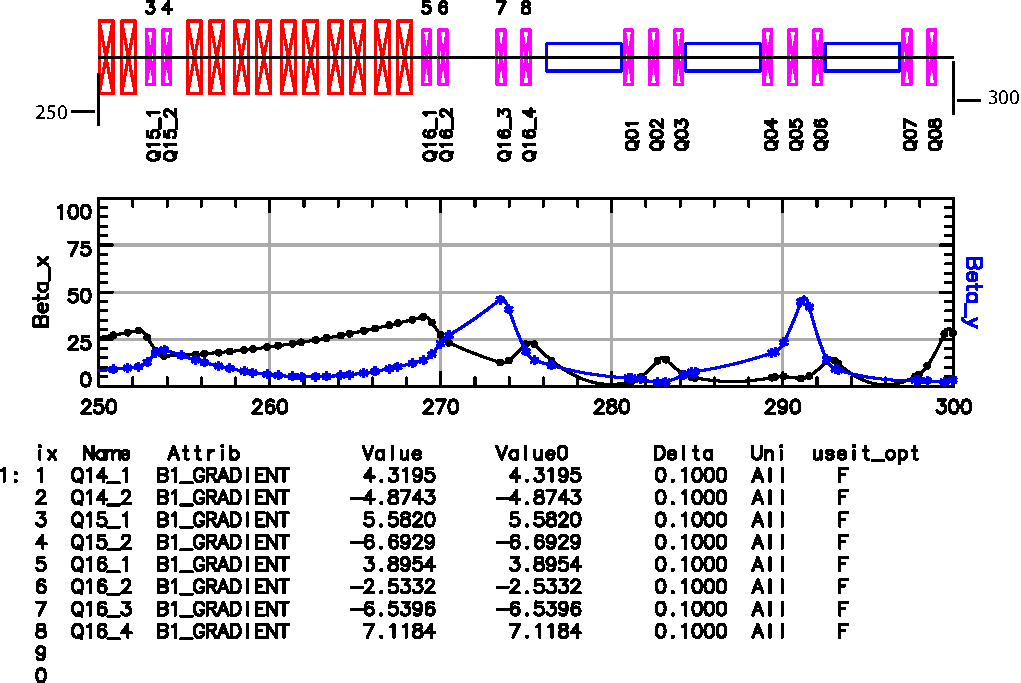
\includegraphics[width=5in]{layout-graph-table.pdf}
  \caption[Example lattice layout and data plots]
{A lattice layout plot (top) above a data plot (middle) which in turn is above a key table plot
(bottom). The points on the curves in the data plot mark the edges of the elements displayed in the
lattice layout. Elements that have attributes that are varied as shown in the key table have the
corresponding key table number printed above the element's glyph in the lattice layout.}
  \label{f:layout.table}
\end{figure}

A lattice layout plot draws the lattice along a straight line with colored rectangles representing
the various elements.  An example is shown in Figure~\ref{f:layout.table}.  The
\vn{tao_template_plot} needed to define a lattice layout looks like:
\index{tao_template_plot}\index{plot!name}
\index{plot!x!min}\index{plot!x!max}\index{plot!n_graph}
\index{tao_template_graph}\index{graph_index}\index{graph!name}
\index{graph!type}\index{graph!title}\index{graph!box}
\index{graph!ix_universe}\index{graph!margin}\index{graph!n_curve}
\begin{example}
  &tao_template_plot
    plot%name        = "<plot_name>"
    plot%n_graph     = <integer>
    plot%x_axis_type = "s"
  /
  &tao_template_graph
    graph_index       = <integer>
    graph%name        = <name>
    graph%type        = "lat_layout"
    graph%title       = "Layout Title"
    plot%box          = <ix>, <iy>, <ix_tot>, <iy_tot>
    graph%ix_universe = <integer> ! -1 => use current default universe
    graph%ix_branch   = <integer> !  0 => use main lattice.
    graph%margin      = <ix1>, <ix2>, <iy1>, <iy2>, "<Units>"
    graph%x%min       = <real>  
    graph%x%max       = <real>  
    graph%y%min       = <real>    ! Default: -100
    graph%y%max       = <real>    ! Default:  100
  /
\end{example}
Example:
\begin{example}
  &tao_template_plot
    plot%name        = "layout"
    plot%n_graph     = 1
    plot%x_axis_type = "s"
  /

  &tao_template_graph
    graph_index       = 1
    graph%name        = "u1"
    graph%type        = "lat_layout"
    graph%box         = 1, 1, 1, 1
    graph%ix_universe = -1  ! Use default universe
    graph%margin      = 0.12, 0.12, 0.30, 0.06, "%BOX"
  /
\end{example}

Which elements are drawn is under user control and is defined using an \vn{lat_layout_drawing}
namelist. See Section~\sref{s:shapes} for more details.

Setting \vn{graph%ix_universe} to -1 means the current default universe will be drawn. Normally, if
there are element shapes that are associated with data or variable shapes (\sref{s:shapes}), these
shapes will be drawn if there are lattice elements associated with the data or variables that live
in the universe with index \vn{graph%ix_universe} and if the associated elements fall within the
range of elements plotted. The exception is that if \vn{graph%ix_universe} is set to -2, the universe
of the associated lattice elements is ignored. Using a value of -2 here only makes sense if the design
lattices of all the universes is the same.

The longitudinal distance markers at either end of the lattice layout can be suppressed by setting
\begin{example}
  graph%x%draw_numbers = F
\end{example}

%-----------------------------------------------------------------
\subsection{Floor Plan Drawing}
\index{floor plan drawing}
\label{s:floor.plan}

\begin{figure}[b]
  \centering
  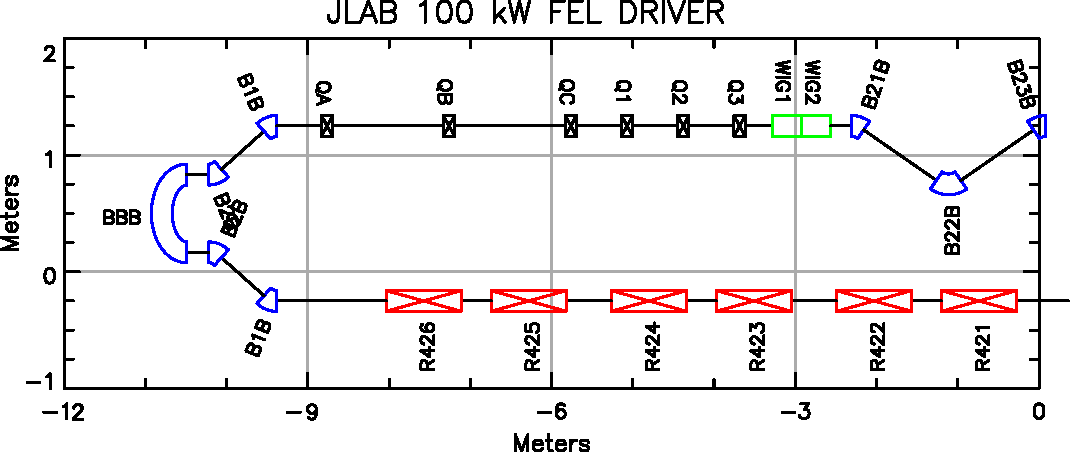
\includegraphics[width=5in]{floor-plan.pdf}
  \caption{Example Floor Plan drawing.}
  \label{f:floor.plan}
\end{figure}

A \vn{floor plan} drawing gives a display of the machine projected onto the horizontal plane.  An
example is shown in Figure~\ref{f:floor.plan}. Like a \vn{Lattice Layout} (\sref{s:lat.layout}),
Elements are represented by colored rectangles and which elements are drawn is determined by a
\vn{floor_plan_drawing} namelist (see~\sref{s:shapes}). Additionally, a cross-section of the walls
of the building containing the machine (\sref{s:building.wall}) can be drawn along with the
reference orbit (which is the closed orbit for machines with a closed geometry). This is illustrated
in Figure~\ref{f:floor.orbit}.

The placement of a lattice element in the drawing is determined by the element's coordinates in the
\vn{global reference system}.  See the Bmad manual for more information on the \vn{global reference
system}.  In the \vn{global reference system}, the $(Z, X)$ plane is the horizontal plane. 

A floor plan orbit is associated with a \vn{graph} of a \vn{plot} (\sref{s:template}). A \vn{graph}
has a \vn{floor_plan} parameter which is a structure of type \vn{tao_floor_plan_struct}. Components
of this structure can be set to control how a floor plan is drawn. The components of a
\vn{tao_floor_plan_struct} are:
\begin{example}
  type tao_floor_plan_struct:
    rotation             = <real>      ! Rotation of floor plan plot: 1.0 -> 360 deg. 
    view                 = "<string>"  ! View plane for floor plan plot. default = "zx"
    correct_distortion   = <logical>   ! Scale plot to use an equal aspect ratio so squares
                                       !   in real space are drawn as squares? Default = T
    flip_label_side      = <logical>   ! Draw element label on other side of element?
    size_is_absolute     = <logical>   ! Shape sizes scaled to absolute dimensions?
    draw_only_first_pass = <logical>   ! Draw only first pass with multipass elements?
    orbit_scale          = <real>      ! Scale for the orbit. Default = 0 => No orbit drawn.
    orbit_color          = "<color>"   ! Line color. Default = "red".
    orbit_pattern        = "<pattern>" ! Line pattern. Default = "solid_line".
    orbit_width          = <integer>   ! Line width. Default = 1.
    orbit_lattice        = "<string>"  ! May be "model" (default), "design", or "base".
\end{example}
A graph is initialized with a \vn{tao_template_graph} namelist (\sref{s:template}). Example:
\begin{example}
  &tao_template_graph
    ...
    graph%floor_plan%rotation = 0.5  ! Rotate 180 degrees
    graph%floor_plan%orbit_scale = 100
    graph%floor_plan%orbit_color = "red"
    graph%floor_plan%orbit_width = 3
    graph%floor_plan%view = "zx"
  /
\end{example}

The \vn{orbit_scale} component scales the displacement of the orbit from the lattice reference
coordinate system (which is the centerline of the lattice elements if there are no
misalignments). So a value of 100.0, a 1~cm orbit is drawn 1~meter from the centerline. A setting of
zero (the default) means that the orbit is now drawn. Note: If \vn{orbit_scale} is not unity, the
plotted orbit when going through a \vn{patch} element with a finite transverse offset will show a
discontinuity due to the discontinuity of the reference orbit.

What plane a floor plan is projected onto is determined by the setting of the
\vn{graph%floor_plan%view} switch. This switch is a two character string.  Each character is either
"x", "y", or "z" and the characters must not be both the same. Default is "zx". The first character
determines which global coordinate is mapped to the horizontal axis of the graph and the second
character determines which global coordinate is mapped to the vertical axis of the graph. There are
six possible two character combinations. The default "zx" setting represents looking at the
horizontal plane from above. A setting of "xz" represents looking at the horizontal plane from
below. The other combinations involving "y" are only potentially useful if the machine has a significant
vertical extent.

To draw multiple orbits representing orbits from \vn{model}, \vn{design}, and/or \vn{base} lattices,
define multiple \vn{graphs} within a \vn{plot}, one for each type of orbit to be displayed and set
the \vn{floor_plan%orbit_lattice} appropriately for each graph.

%----------------
\begin{figure}[b]
  \centering
  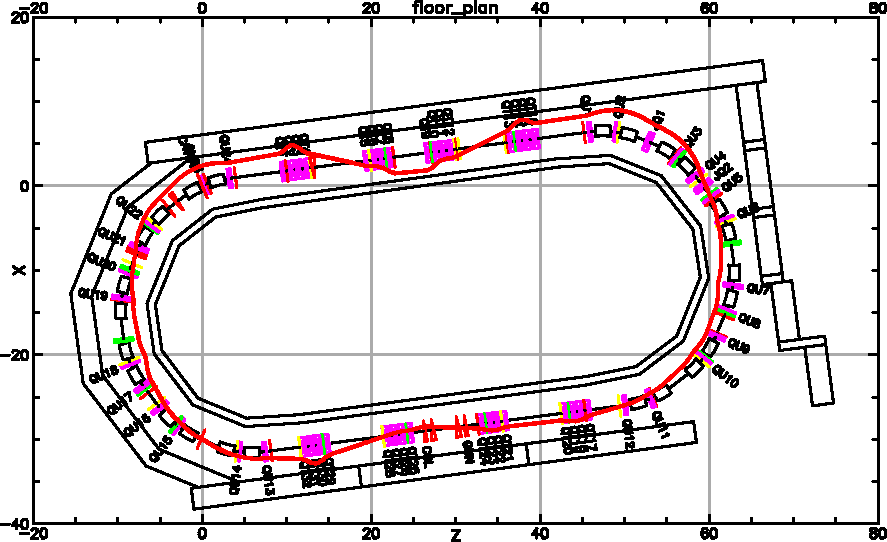
\includegraphics[width=5in]{floor-plan-orbit.pdf}
  \caption[Floor plan with orbit and building walls.]{Example Floor plan drawing with the closed orbit 
(red line) and building walls included.}
  \label{f:floor.orbit}
\end{figure}
%----------------

If element labels are to be drawn, on which side the labels are drawn can be flipped by setting 
\vn{graph%floor_plan%flip_label_side} to True.

The \vn{size_is_absolute} logical is combined with the \vn{<size>} setting for a shape to determine the
size transverse to the center line curve of the drawn shape (\sref{s:shapes}).
If \vn{size_is_absolute} is False (the default), \vn{<size>} is taken to be the size of
the shape in points (72 points is approximately 1 inch). If \vn{size_is_absolute} is True,
\vn{<size>} is taken to be the size in meters. That is, if \vn{size_is_absolute} is
False, zooming in or out will not affect the size of an element shape while if
\vn{size_is_absolute} is True, the size of an element will scale when zooming.

An overall rotation of the floor plan can be controlled by setting \vn{rotation} parameter. A
setting of 1.0 corresponds to 360$^\circ$. Positive values correspond to counter-clockwise
rotations.  Alternatively, the global coordinates at the start of the lattice can be defined in the
lattice file and this can rotate the floor plan.  Unless there is an offset specified in the lattice
file, a lattice will start at $(x, y) = (0, 0)$. Assuming that the machine lies in the horizontal
plane with no negative bends, the reference orbit will start out pointing in the negative $x$
direction and will circle clockwise in the $(x, y)$ plane.

The \vn{draw_only_first_pass} logical, if set True, suppresses drawing of \vn{multipass_slave}
lattice elements that are associated with the second and higher passes. This logical defaults to
False. Setting to True is only useful in some extreme circumstances where the plotting of additional
passes leads to large pdf/ps file sizes.

Note: If \vn{graph%ix_universe} is set to -1 the current viewed universe is used. If
\vn{graph%ix_universe} is set to -2, all universes are plotted.

Example Floor Plan template:
\begin{example}
  &tao_template_plot
    plot%name = "floor"
    plot%n_graph = 1
  /

  &tao_template_graph
    graph_index = 1
    graph%name = "1"
    graph%type = "floor_plan"
    graph%box = 1, 1, 1, 1
    graph%margin = 0.10, 0.10, 0.10, 0.10, "%BOX"
    graph%ix_universe = -2   ! Draw all universes.
    graph%x%min = -12  
    graph%x%max = 0    
    graph%x%major_div_nominal = 4
    graph%x%minor_div = 3
    graph%x%label = "SMART LABEL"
    graph%y%label = "SMART LABEL"
    graph%y%max = 2  
    graph%y%min = -1 
    graph%floor_plan%correct_distortion = T
    graph%floor_plan%size_is_absolute = T
    graph%floor_plan%view = "xz"  ! Looking from beneath
    graph%floor_plan%orbit_scale = 100
  /
\end{example}

Having \vn{graph%x%label} and \vn{graph%y%label} set to ``\vn{SMART LABEL}'' means that the actual axis labels will be 
picked appropriately based upon the setting of \vn{graph%floor_plan%view}.

To prevent the drawing of the axes set \vn{graph%draw_axes} to False.  To prevent the drawing of a
grid at the major division points set \vn{graph%draw_grid} to False.

By default, the horizontal or vertical margins of the graph will be increased so that the horizontal
scale (meters per plotting inch) is equal to the vertical scale. That is, both axes will have an
equal aspect ratio and squares in real space will be drawn as squares in the plot. If
\vn{graph%floor_plan%correct_distortion} is set to \vn{False}, this scaling will not be done.

Note: The \vn{show ele -floor} command (\sref{s:show}) can be used to view an element's global
coordinates.

%-----------------------------------------------------------------
\subsection{Lat_layout and Floor_plan Drawings Shape Definition}
\label{s:shapes}
\index{lat_layout drawings}
\index{floor_plan drawings}

\vn{Floor plan} (\sref{s:floor.plan}) and \vn{lattice layout} drawings use various shapes, sizes,
and colors to represent lattice elements. The association of a particular element with a given shape
is determined via two namelists: \vn{lat_layout_drawing} for the lattice layout and
\vn{floor_plan_drawing} for floor plan drawings.  Two different namelists are used since, for
example, a size that is good for a layout will not necessarily be good for a floor plan.

The file that \tao looks in to find these two namelists is set by the first file specified in the
\vn{plot_file} array set in the \vn{tao_start} namelist (\sref{s:init.begin}). The default, if
\vn{plot_file} is not set, is the root initialization file.

The namelist syntax is the same for both:
\begin{example}
  &lat_layout_drawing
    include_default_shapes = <logical>
    ele_shape(N) = "<ele_id>" "<shape>" "<color>" "<size>" "<label>" <draw> 
                                                          <multi> <line_width> <offset>
  /

  &floor_plan_drawing
    ... same as lat_layout_drawing ...
  /
\end{example}
For Example:
\begin{example}
  &floor_plan_drawing
    include_default_shapes = T
    !               ele_id                  Shape        Color     Size  Label  ..etc..
    ele_shape(1) = "quadrupole::q*"         "box"        "red"     0.75  "name"  
    ele_shape(2) = "quadrupole::*"          "xbox"       "red"     0.75  "none" 
    ele_shape(3) = "sbend::sb*"             "box"        "blue"    0.37  "none"
    ele_shape(4) = "sbend::*"               "box"        "blue"    0.37  "none"  
    ele_shape(5) = "wiggler::*"             "xbox"       "green"   0.50  "name"
    ele_shape(6) = "var::quad_k1"           "circle"     "purple"  0.25  "name"
    ele_shape(7) = "data::orbit.x|design"   "vvar:box"   "orange"  0.25  "name"
    ele_shape(8) = "building_wall::*"       "solid_line" "black"    0    "none"
    ele_shape(3)%multi = T
    ele_shape(5:6)%line_width = 5, 6
  /
\end{example}
A figure is drawn for each lattice element in the lattice that matches the \vn{<ele_id>} field
(\sref{s:ele.list.format}). Thus, in the example above, \vn{ele_shape(1)} will match to all
quadrupoles whose name begins with ``q'' and \vn{ele_shape(2)} will match all quadrupoles.

Besides the usual element class prefixes (\vn{quadrupole::}, \vn{sbend::}, etc.), other prefixes
that can be used with an \vn{<ele_id>} are
\begin{example}
  data::            ! Match to \tao datum name.
  var::             ! Match to \tao variable name.
  alias::           ! Match to lattice element alias parameter.
  type::            ! Match to lattice element type parameter.
  building_wall::   ! Used in floor_plan plots.
\end{example}
The \vn{data::} prefix is used to match to data that will be used in an optimization. Thus, in the
above example, \vn{ele_shape(7)} specifies that an ``x'' will be drawn at points where there is
valid \vn{orbit.x} data. For this to work, an \vn{orbit.x} data array must be defined
(\sref{s:init.data}).

The \vn{var::} prefix is used for drawing variable locations for variables used in an
optimization. In the above example, it is assumed that a \vn{quad_k1} variable array has been
setup. A circle will be drawn at each element under control of a \vn{quad_k1} variable.

For \vn{floor_plan} drawings, the building wall (\sref{s:building.wall}) can be drawn by specifying
an \vn{ele_shape} whose name is \vn{"building_wall::<name>"} where \vn{<name>} is used to match to
the building wall section name. Use ``\vn{*}'' for \vn{<name>} to match to all names. For the
building wall, the only attribute that is relevant is the \vn{<color>} attribute.

The \vn{alias::} and \vn{type::} prefixes for \vn{<ele_id>} are used to match to the \vn{alias} and
\vn{type} string parameters of that can be set in the lattice file for each individual element.

If an element matches more than one shape,
what is drawn depends upon the setting of \vn{<multi>}. If \vn{<multi>} is False (the default) for
the first shape matched in the list of shapes, only this shape will be used.  If \vn{<multi>} is
True, \tao will draw this shape and then look for additional matches. Each time an additional match
is found, the shape is drawn and the setting of \vn{<multi>} for that shape will be used to
determine whether additional shapes are searched for. Thus \vn{<multi>} can be use to draw, for
example, a \vn{circle} shape superimposed upon a \vn{bow_tie} shape.

\tao defines a set of default shapes in case no shapes are defined in the plot file. If the
optional \vn{include_default_shapes} logical, which can be set for either \vn{floor_plan} and/or
\vn{lat_layout} shape namelists, is set to False (the default), the default shapes are not used.
If \vn{include_default_shapes} is set to True, the default shapes are appended to the list of 
shapes.

Use the \vn{show plot -floor_plan} and \vn{show plot -lat_layout} commands to see the defined
shapes. Use the \vn{set floor_plan} and \vn{set lat_layout} commands (\sref{s:set})) to set shape
parameters on the command line.

The width of a drawn shape is the width of the associated element. The exception is the \vn{"x"}
shape whose width is always the same as the height determined by the \vn{<size>} setting.

\vn{<size>} is the half height of the shape. That is, the size transverse to the longitudinal
dimension. For \vn{lat_layout} drawings, \vn{<size>} = 1.0 corresponds to full scale if the default
\vn{graph%y%min} = -1 and \vn{graph%y%max} = 1 are used. For {floor_plan} drawings, the drawn size
is also affected by the setting of \vn{graph%floor_plan%size_is_absolute} See \sref{s:floor.plan}
for more details.

The overall size of all the shapes can be scaled using the \vn{plot_page} (\sref{s:init.plot})
parameters
\begin{example}
  floor_plan_shape_scale     ! For floor_plan drawings. Default = 1
  lat_layout_shape_scale     ! For lat_layout drawings. Default = 1
\end{example}

The text size in both \vn{floor_plan} and \vn{lat_layout}
plots can be scaled by using the \vn{plot_page} parameter
\begin{example}
  legend_text_scale          ! Default = 1
\end{example}
Use the \vn{show plot} command to view these parameters. Use the
\vn{set plot_page} command to set these parameters.

\vn{<color>} is the color of the shape. Good colors to use are:
\index{element shape!color}
\begin{example}
  "black"
  "blue"
  "cyan"
  "green"
  "magenta"
  "orange"
  "purple"
  "red"
  "yellow"
\end{example}

The \vn{<line_width>} parameter is an integer that specifies the width of the lines drawn. The
default is 1.

The \vn{<offset>} parameter offsets the shape transverse to the reference orbit.

The \vn{<label>} indicates what type of label to print next to the corresponding
element glyph. Possibilities are:
\begin{example}
  name            -- The element name (default).
  none            -- No label is drawn.
  s               -- Draw longitudinal s position.
\end{example}
The default is \vn{"name"}

The \vn{<draw>} field determines if a shape is drawn or not. The default is \vn{T}. This can be
useful for toggling on and off the drawing of shapes using the \vn{set shape} command
(\sref{s:set}).

Note: There is an old, deprecated syntax where both the lattice layout and floor plan drawings are
specified via one \vn{element_shapes} namelist.

The \vn{<shape>} parameter is the shape of the figure drawn. The \vn{<shape>} string will have the
form:
\begin{example}
  <shape-name>  or
  <prefix>:<shape-name>  
\end{example}
Valid \vn{shape-name}s are: 
\index{box}\index{xbox}
\begin{example}
  "box"            -- Rectangular box
  "bow_tie"        -- Bow-tie shape.
  "circle"         -- Circle centered at center of element.
  "diamond"        -- Diamond shape.
  <pattern_name>   -- Custom shape specified by <name>. Used with "pattern" prefix.
  "rbow_tie"       -- Bow-tie shape rotated 90 degrees.
  "d_triangle"     -- Triangle pointing ``down''.
  "l_triangle"     -- Triangle pointing ``left'' (upstream).
  "r_triangle"     -- Triangle pointing ``right'' (downstream).
  "u_triangle"     -- Triangle pointing ``up''. 
  "x"              -- "X" centered at center of element
  "xbox"           -- Rectangular box with an x through it.
  "dashed_line"    -- Only used with ele_id set to "building_wall".
  "dash_dot_line"  -- Only used with ele_id set to "building_wall".
  "dotted_line"    -- Only used with ele_id set to "building_wall".
  "solid_line"     -- Only used with ele_id set to "building_wall".
\end{example}
Valid prefixes are:
\begin{example}
  "asym_var"   -- Like "var" prefix but is not symmetric about the center line.
  "asym_vvar"  -- Like asym_var except scaled to associated variable or datum.
  "pattern"    -- Custom shape. <shape-name> here is a pattern name.
  "var"        -- Shape with variable height. 
                       The shape size is symmetric about the center line.
  "vvar"       -- Like "var" prefix except scaled to associated variable or datum.
\end{example}

For example, if an element's shape is set to \vn{var:box} or \vn{asym_var:box}, the drawn size of the
element is proportional to the element's magnetic or electric strength. The associated
\vn{<size>} setting is the multiplier used to scale from element strength to height. For
example, for a quadrupole the height is proportional to the \vn{K1} focusing strength. The
difference between \vn{var:box} or \vn{asym_var:box} is that with \vn{var:box} the drawn
box is symmetric with respect to the centerline with a size independent of the sign of the
element strength. On the other hand, with \vn{asym_var:box}, the drawn box will terminate
with one side on the centerline and the side on which it is drawn will depend upon the the
sign of the element strength. Note: Not all lattice elements can be used with a
\vn{var:box} or \vn{asym_var:box}.

A \vn{vvar:box} shape is like a \vn{var:box} and a \vn{asym_vvar:box} is like a
\vn{asym_var:box}. The difference is that \vn{vvar:box} and \vn{asym_vvar:box} shapes may only be
used when the \vn{<ele_id>} is associated with data or variables. That is, when the \vn{<ele_id>}
string starts with ``\vn{data::}'' or ``\vn{var::}''. In this case, the height of the box, instead
of being proportional to the strength of the element, is proportional to the value of the associated
datum or variable. If no datum or variable component is specified in the \vn{ele_id}, the model
value will be used. Thus, in the above example, where \vn{<ele_id>} was set to
\vn{"data::orbit.x|design"}, the design value is used.

The \vn{solid_line}, \vn{dashed_line}, \vn{dash_dot_line}, and \vn{solid_line} settings for
\vn{<shape>} is used when \vn{<ele_id>} is set to \vn{building_wall} to indicate what type of line
is to be drawn.

The \vn{pattern:<pattern_name>} shape allows for a custom pattern to be specified. Custom
patterns are specified by a \vn{shape_pattern} namelist:
\begin{example}
  &shape_pattern
    name = "<curve_name>"
    line%width = <line_width>
    pt(1) = <s>, <y>
    pt(2) = <s>, <y>
    pt(3) = ...
  /
\end{example}
with \vn{<s>} being the longitudinal coordinate and \vn{<y>} begin the coordinate perpendicular to the
longitudinal coordinate.
Example:
\begin{example}
  &floor_plan_drawing
    ...
    ele_shape(2) = "quadrupole::*"     "pattern:q_pat"     "red"     0.75     "none" 
    ...
  /

  &shape_pattern
    name = "q_pat"
    pt(1) = 0, -1
    pt(2) = 1, -1
    pt(3) = 0.9, 1
    pt(4) = 0.1, 1
    pt(5) = 0, -1
  /
\end{example}
The \vn{name} of the \vn{shape_pattern} namelist (in this example it is "q_pat") must match the name
given by \vn{"pattern:<pattern_name>"}. The pattern is specified by a number of points. Between the
points, a line segment is drawn. In the above example, the pattern is an isosceles trapezoid.  When
drawn, the \vn{s} coordinate is scaled so that $s = 0$ corresponds to the entrance end of the
element and $s = 1$ corresponds to the exit end. The \vn{y} coordinate is scaled by the \vn{size}
attribute of the \vn{ele_shape}. The color of the line segments is set by the definition and the width
of the line segments is set by the pattern definition. Multiple \vn{shape_pattern}s with the same name
can be defined. In such a case, all patterns of a given name will be drawn. This allows the construction
of more complex patterns. For example, a rectangle and a triangle drawn together.

%-----------------------------------------------------------------
\subsection{Aperture Drawing}
\index{aperture drawing}
\label{s:draw.ap}

\begin{figure}
  \centering
  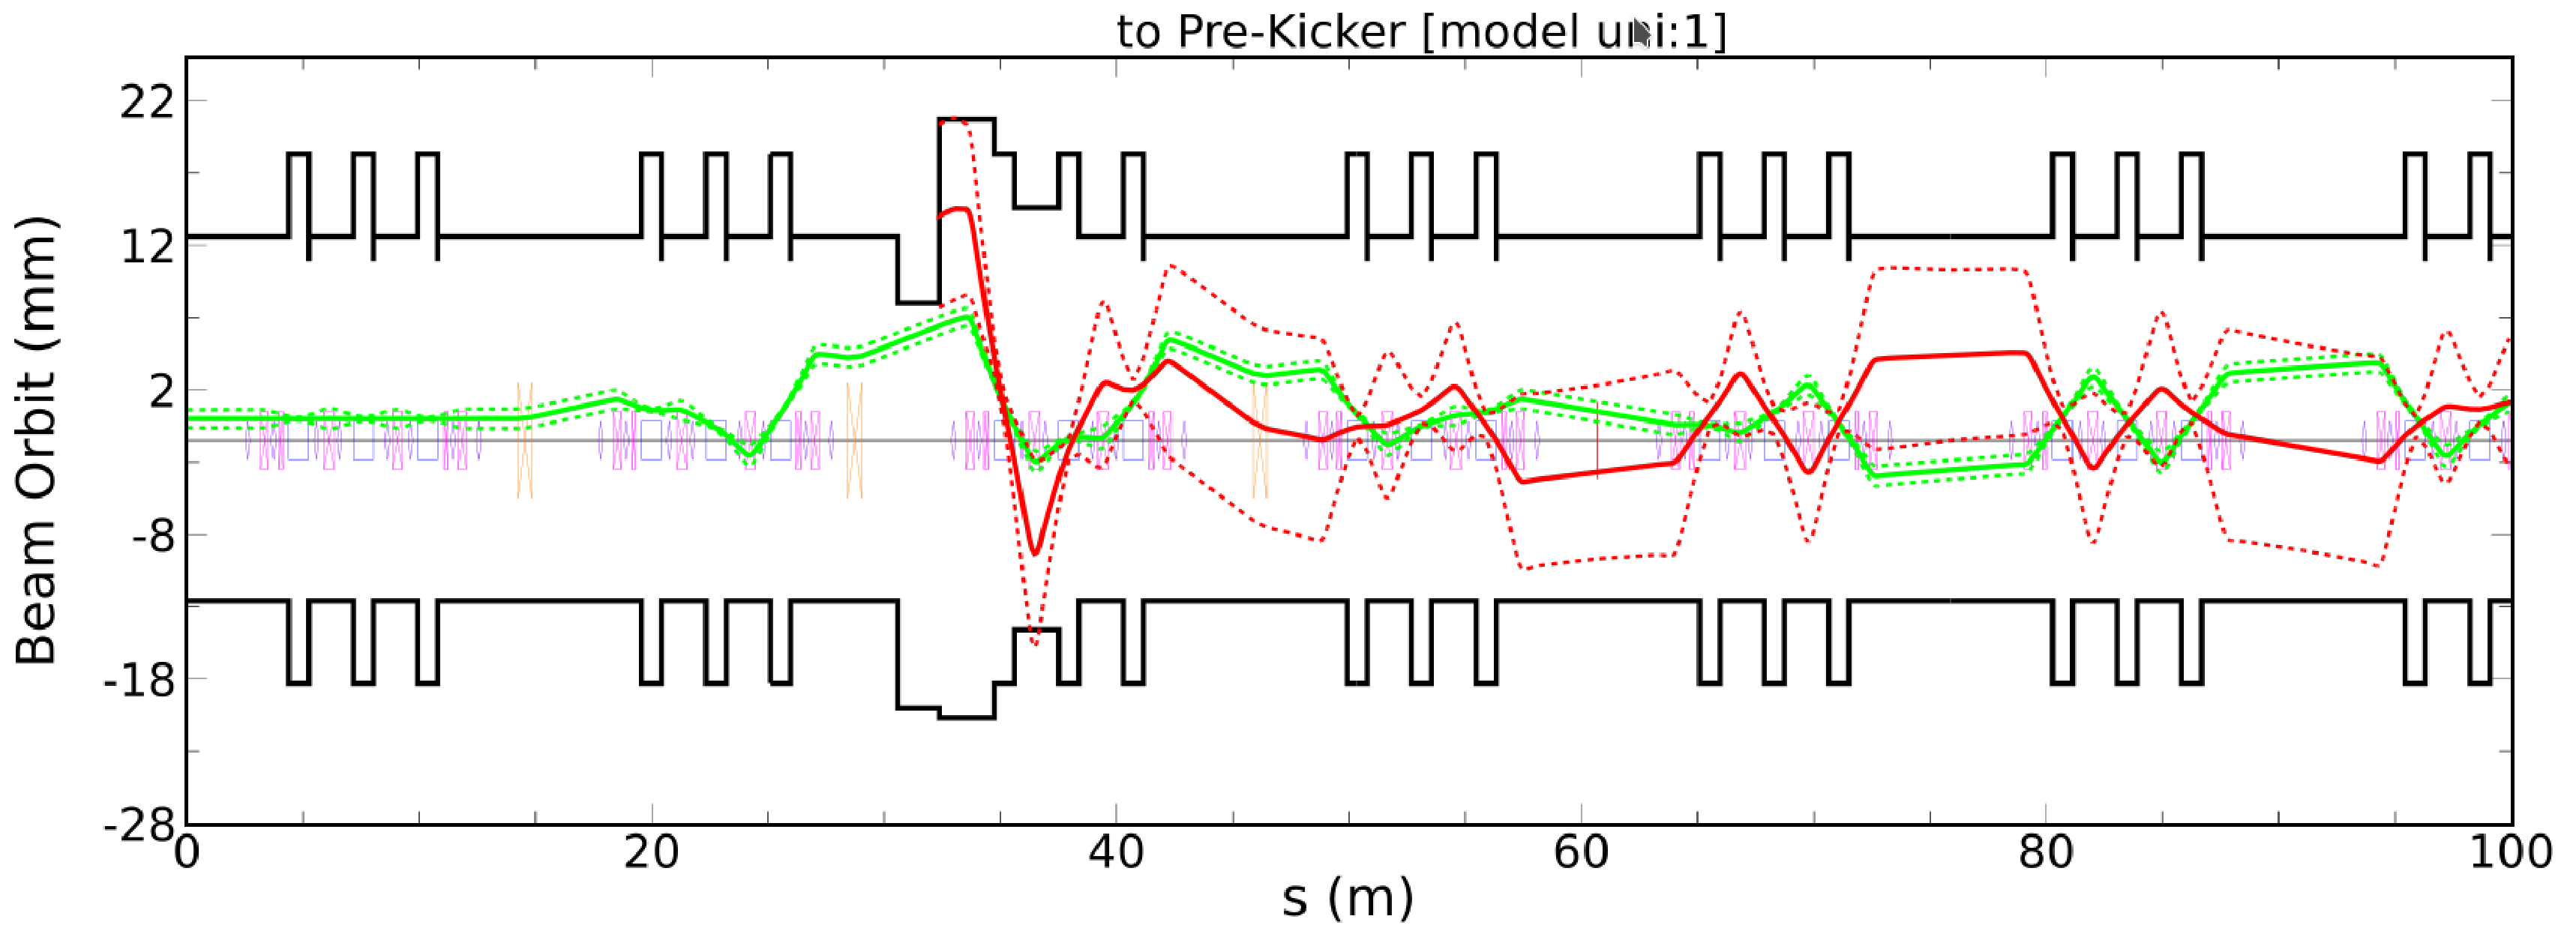
\includegraphics[width=6in]{aperture-plot.pdf}
  \caption[Example beam aperture plot.]
{Example plot of the beam aperture. In this drawing, two turns of three injected particles are drawn. The
particles start at different positions and illustrate what the size of an injected beam would be. Also drawn
(a bit faint) is a \vn{lat_layout} showing lattice element positions.}
  \label{f:aperture}
\end{figure}

Beam apertures can be defined in the \bmad lattice file. Apertures can be defined in one of three
ways. The most common is to set limit or aperture parameters for an element. Another possibility 
is to use a \vn{mask} element (which can be used to define an aperture of arbitrary shape). The
third possibility involves defining a continuous three-dimensional wall. This third possibility 
is only used with Runge-Kutta type tracking. 

To simplify things, the drawing of the beam aperture ignores any \vn{mask} elements (since the
geometry can be very complicated here) and ignores any three-dimensional walls (which are only
used for Runge-Kutta type tracking). \fig{f:aperture} shows an example of a aperture drawing.

To draw an aperture, a curve's \vn{data_source} parameter must be set to \vn{"aperture"} and the \vn{data_type} parameter is set to one of
\begin{example}
  "+x"     ! Aperture in +X direction
  "-x"     ! Aperture in -X direction
  "+y"     ! Aperture in +Y direction
  "-y"     ! Aperture in -Y direction
\end{example}
The apertures in the $+x$ and $+y$ directions will have positive values and the apertures in the
$-x$ and $-y$ directions will have negative values. Set the curve's \vn{y_axis_scale_factor} to scale
the aperture curve if needed.

The following example will graphs the horizontal orbit along with the horizontal apertures.
\begin{example}
  &tao_template_plot
    plot%name        = "x_orbit"
    plot%x_axis_type = "s"
    plot%n_graph     = 1
  /

  &tao_template_graph
    graph%name    = "x"
    graph_index   = 1

    curve(1)%data_source  = "aperture"
    curve(1)%data_type    = "+x"
    curve(1)%draw_symbols = T
    curve(1)%draw_line    = F
    curve(1)%data_source  = "aperture"
    curve(2)%data_type    = "-x"
    curve(2)%draw_symbols = T
    curve(2)%draw_line    = F
    curve(3)%data_type = "orbit.x"
  /
\end{example}
Note: Aperture curves will ignore the \vn{curve%component} parameter.

\begin{figure}
  \centering
  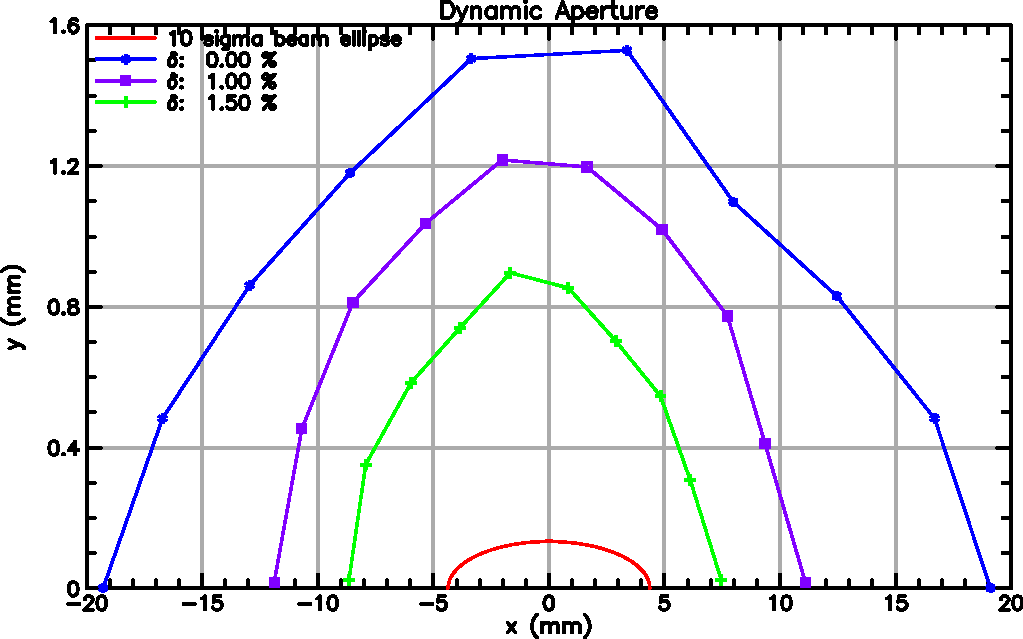
\includegraphics[width=5in]{dynamic-aperture.pdf}
  \caption{Example dynamic aperture plot.}
  \label{f:da-plot}
\end{figure}

%-----------------------------------------------------------------
\subsection{Dynamic Aperture Curve Drawing}
\index{dynamic aperture drawing}
\label{s:da.plot}

A \vn{dynamic_aperture} drawing displays the results of the dynamic aperture calculation (\sref{s:da.calc}).
Example plot setup:
\begin{example}
&tao_template_plot
  plot%name = "da"
  plot%x_axis_type = "phase_space"
  plot%n_graph = 1
/

&tao_template_graph
  graph%name = "g1"
  graph%type = "dynamic_aperture"
  graph_index = 1
  graph%x%label = "x (mm)"
  graph%x_axis_scale_factor = 1000  ! Plot in mm.
  graph%y%label = "y (mm)"
  curve(1)%line%color = "red"
  curve(1)%data_type = 'beam_ellipse'
  curve(1)%line%width = 5
  curve(1)%legend_text = '10 sigma beam ellipse'
  curve(1)%draw_symbols = F
  curve(1:10)%y_axis_scale_factor = 10*1000  ! Plot in mm.
  curve(2:10)%draw_symbols = 9*T
  curve(2:10)%data_type = 9*"dynamic_aperture"
  curve(2:10)%data_index = 1, 2, 3, 4, 5, 6, 7, 8, 9
  curve(3)%symbol%color = "purple"
  curve(3)%line%color = "purple"
/
\end{example}
This will produce a plot similar to Fig.~\ref{f:da-plot}.  Each curve represents a dynamic aperture
scan at fixed initial momentum $p_z$.

Dynamic aperture curves can have the following \vn{%data_type} parameters:
\begin{example}
  "dynamic_aperture"        ! Curve points are with respect to the closed orbit (x,y).
  "dynamic_aperture_ref0"   ! Curve points are with respect to x = y = 0.
  "beam_ellipse"            ! Draws the beam ellipse within the [min_angle, max_angle] range.
  "beam_ellipse_full"       ! Draws the entire beam ellipse.
\end{example}

In the above example, the first curve has \vn{%data_type} set to \vn{"beam_ellipse"}. This results
in the half ellipse in red since the [min_angle, max_angle] set in the \vn{tao_dynamic_aperture}
namelist for this example was [0, pi]. If the entire ellipse is desired to be drawn, the
\vn{%data_type} can be set to \vn{"beam_ellipse_full"}. The scale of the ellipse drawn is set by the
\vn{ellipse_scale} parameter of the \vn{tao_dynamic_aperture} namelist (\sref{s:da.calc}). The default value is
10 so that a $10 \, \sigma$ ellipse will be drawn by default. Also used in calculating the ellipse
curve are the settings of \vn{a_emit} and \vn{b_emit} emittances also set in the same namelist.

There are 10 curves defined in the example. Curves 2 through 10 have \vn{%data_type} set to
\vn{"dynamic_aperture"}. Each curve here represents one dynamic aperture scan. The scan index is set
by a curve's \vn{%data_index} parameter. An index of "1" denotes the first scan with the initial
momentum set by the first value in the \vn{pz} array set in the \vn{tao_dynamic_aperture} namelist
(\sref{s:da.calc}). If a curve has an index that is greater than the number of scans, that curve is ignored.

%-----------------------------------------------------------------
\subsection{Histogram Drawing}
\index{histogram drawing}
\label{s:histogram}

A \vn{histogram} drawing displays a histogram of phase space beam density. Histogram plotting is
associated with a \vn{graph} by setting \vn{graph%type} equal to \vn{"histogram"}. The concepts here
are similar to \vn{phase space} plotting (\sref{s:phase.space}). An example is shown in
Fig.~\ref{f:histogram}, using the example histogram template:
\begin{example}
&tao_template_plot
  plot%name = "zhist"
  plot%n_graph = 1
/

&tao_template_graph
  graph_index = 1
  graph%name = "z"
  graph%type = "histogram"
  graph%box = 1, 1, 1, 1
  graph%title = "Bunch Histogram: Z"
  graph%margin =  0.15, 0.06, 0.12, 0.12, "%BOX"
  graph%x%min = -6
  graph%x%max =  6
  graph%x%label = "z (mm)"
  graph%y%label = "Current (A)"
  graph%y%label_offset = .1
  graph%x_axis_scale_factor = 1000.00 !m->mm

  curve(1)%hist%density_normalized = T
  curve(1)%hist%weight_by_charge = T
  curve(1)%hist%number = 100
  curve(1)%line%color = "blue"
  curve(1)%line%pattern = "dashed"
  curve(1)%y_axis_scale_factor = 299792458  !Q/m * c_light
  curve(1)%data_type = "z" 
  curve(1)%data_source = "beam_tracking"
  curve(1)%ele_ref_name = "BEGINNING"
  curve(1)%symbol%type = "dot"
/
\end{example}

\begin{figure}
  \centering
  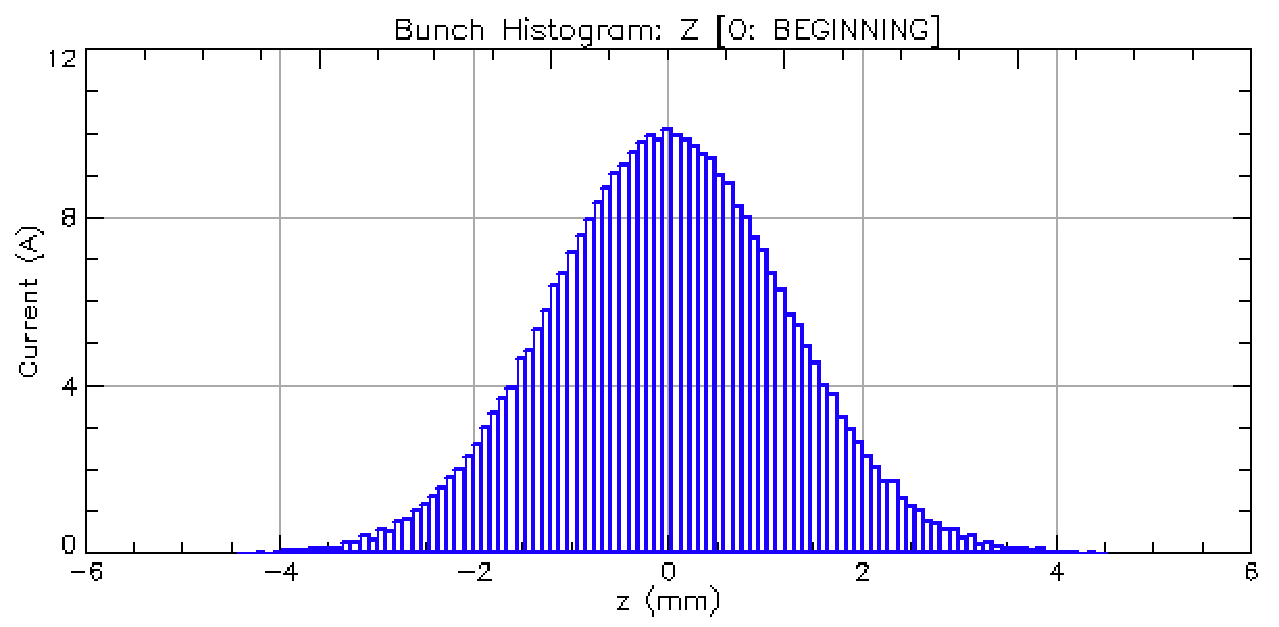
\includegraphics[width=5in]{histogram.pdf}
  \caption{Example histogram plot.}
  \label{f:histogram}
\end{figure}

For a \vn{"histogram"} type graph, \vn{curve%data_type} determines what coordinate is plotted along
the x-axis.  Valid \vn{curve%data_type} values are:
\index{x}\index{px}\index{y}\index{py}\index{z}\index{pz}
\begin{example}
  "x", "px", "y", "py","z", "pz"   -- Phase space coordinates
  "intensity"                      -- Photon total intensity 
  "intensity_x"                    -- Photon intensity along x-axis 
  "intensity_y"                    -- Photon intensity along y-axis
  "phase_x"                        -- Photon phase along x-axis
  "phase_y"                        -- Photon phase along y-axis
\end{example}
In this example above, the $x$-axis of the plot will correspond to the $z$ phase space coordinate.

The maximum and minimum of the bins is set automatically to fit the data.  The
\vn{curve%hist%number} establishes the number of bins. Alternatively, if \vn{curve%hist%number = 0},
then \vn{curve%hist%width} establishes the width of the histogram bins and sets the number
automatically.

If \vn{curve%hist%density_normalized = T}, then the height of a bin will be divided by its width. If
\vn{curve%hist%weight_by_charge = T}, then the particle charge will be used to bin, otherwise the
particle count will be used to bin.

The \vn{curve%hist%center} will insure that a bin will be centered at this location.

\index{curve!ele_ref_name}
To change the place in the lattice where the data for the \vn{histogram} is evaluated, use the
\vn{set curve ele_ref_name} command.

If \vn{graph%type} is \vn{"histogram"} then \vn{curve%data_source} 
must be either:
\begin{example}
  "beam"
  "multi_turn_orbit"
  "rel_multi_turn_orbit"
\end{example} 
\vn{"beam"} indicates that the points of the histogram plot will be obtained correspond to the
positions of the particles within a tracked beam. 

Setting \vn{curve%data_source} to \vn{"multi_turn_orbit"} or \vn{"rel_multi_turn_orbit"} is used for
rings where a single particle is tracked multiple turns and the position of this particle is
recorded each turn. The number of turns is determined by the setting of \vn{curve%n_turn}. The
starting position for the tracking is set by setting the \vn{particle_start[x]},
\vn{particle_start[px]}, etc.  parameters in the lattice file (see the \bmad manual for
details). The difference between \vn{"multi_turn_orbit"} and \vn{"rel_multi_turn_orbit"} is that
\vn{"rel_multi_turn_orbit"} is drawn relative to the phase space point
\begin{equation}
  p_{z0} \cdot (\eta_x, \eta'_x, \eta_y, eta'_y, 0, 0)
\end{equation}
where $p_{z0}$ is the value of the particle's initial $p_z$ and $\eta$ is the dispersion at the
reference element where the orbit is being evaluated for the plot.

%%-----------------------------------------------------------------
%\subsection{Beam Chamber Wall Drawing}
%\index{beam chamber wall}
%\label{s:beam.wall.draw}
%
%If a beam chamber wall has been defined in the lattice file, This wall can be drawn in a \vn{curve}
%by setting \vn{curve%type} to \vn{"beam_chamber_wall"}.
%
%Beam chamber walls are drawn, like a \vn{lat_layout}, on a one dimensional line as a function of
%longitudinal position along the machine centerline.
%
%Note: Use the command \vn{show ele -wall} to print information about the beam chamber wall for a
%particular element.

%%-----------------------------------------------------------------
%\subsection{ Controller Element Curve Drawing}
%\index{drawing controller element curves}
%\label{s:draw.control}
%
%A controller element is a \bmad lattice element that controls the parameters of other elements.
%There are three types of controller elements: \vn{groups}, \vn{overlays}, and \vn{rampers}. See 
%the Bmad manual for more details. A controller has one or more independent variables that control
%parameters of other elements. The response of a controlled parameter as a function of any one of 
%controller variables may be plotted.

%% Put under graph%type:
%%  "control_curve"      ! Plot slave response for a controller lattice element (\sref{s:draw.control})


%-----------------------------------------------------------------
\subsection{Key Table Drawing}
\index{key table}
\label{s:key.table}

A \vn{key table} displays information about variables bound to keyboard keys \sref{s:key.bind}. Key
bindings are used in \vn{single mode}. An example is shown in Figure~\ref{f:layout.table}. A
template to create a key table looks like:
\begin{example}
  &tao_template_plot
    plot%name = "table" 
    plot%n_graph = 1
  /

  &tao_template_graph
    graph%type = "key_table" 
    graph_index = 1
  /
\end{example}

The number in the upper left corner, to the left of the first column, (\vn{1} in
Fig.~\ref{f:layout.table}) shows the active \vn{key bank}. The columns in the Key Table are:
\begin{example}
  Ix         ! Key index.
  Name       ! Element name whose attribute is bound.
  Attrib     ! Name of the element attribute that is bound.
  Value      ! Current value of bound attribute.
  Value0     ! Initial value of bound attribute.
  Delta      ! Change in value when the appropriate key is pressed.
  Uni        ! Universe that contains the element.
  Opt        ! Shows if bound attribute is used in an optimization.
\end{example}

Note that in a \vn{Lattice Layout}, if a displayed element has a bound attribute, then the key index
number will be displayed just above the element's glyph.

The \vn{key_table} is drawn with respect to the upper left hand corner of the region in which it is
placed.

%-----------------------------------------------------------------
\subsection{Phase Space Plotting}
\index{phase space plotting}
\label{s:phase.space}

\begin{figure}
  \centering
  \begin{subfigure}[b]{0.45\textwidth}
    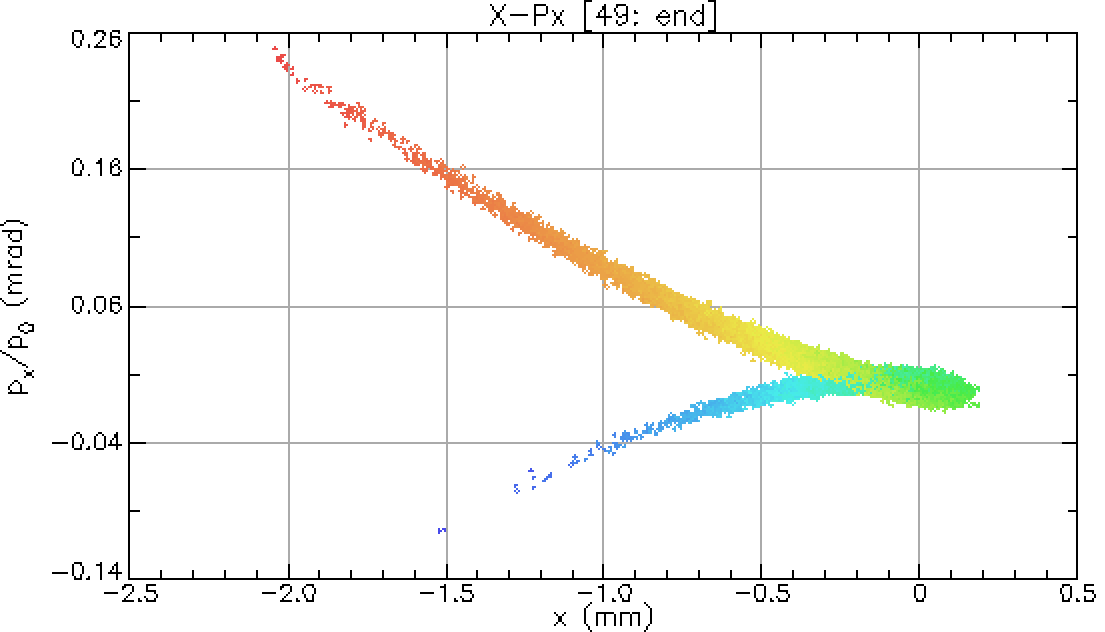
\includegraphics[width=\textwidth]{plot-color-xpx}
    \caption{Horizontal phase space}
  \end{subfigure}
  \begin{subfigure}[b]{0.45\textwidth}
    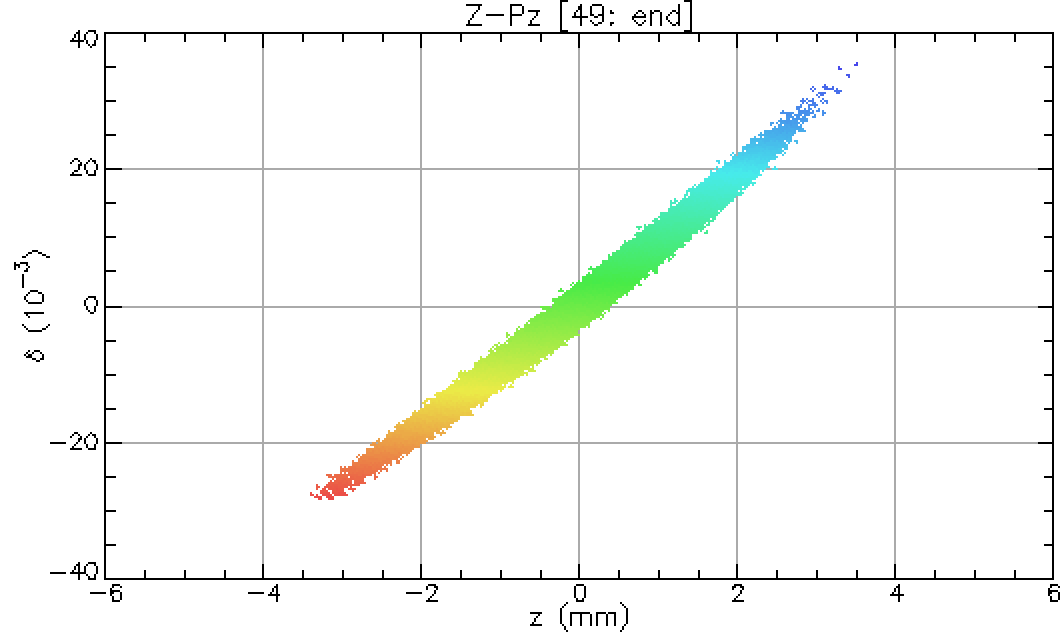
\includegraphics[width=\textwidth]{plot-color-zpz}
    \caption{Longitudinal phase space}
  \end{subfigure}  
  \caption{Example Phase Space plot, with points colored by the \vn{pz} coordinate.}
  \label{f:phase.space}
\end{figure}

A \vn{phase space} plot displays a particle or particles phase space coordinates at a given
location. Phase space plotting is associated with a \vn{graph} by setting \vn{graph%type} equal to
\vn{"phase_space"}. The concepts here are similar to \vn{data} plotting (\sref{s:graph.types}). An
example is show in Figure~\ref{f:phase.space}.  Example Phase Space template:
\begin{example}
&tao_template_plot
  plot%name = "xphase"
  plot%n_graph = 1
/

&tao_template_graph
  graph_index = 1
  graph%name = "x"
  graph%type = "phase_space"
  graph%box = 1, 1, 1, 1
  graph%title = "X-Px"
  graph%margin =  0.15, 0.06, 0.12, 0.12, "%BOX"
  graph%x%min =   -2.5
  graph%x%max = 0.5
  graph%x%label = "x (mm)"
  graph%x_axis_scale_factor = 1000.00 !m->mm
  graph%y%label =  "p\textbackslash{}dx\textbackslash{}u/p\textbackslash{}d0\textbackslash{}u (mrad)"
  graph%y%major_div = 4
  graph%y%label_offset=.4
  curve(1)%data_type_x = "x" 
  curve(1)%data_type   = "px" 
  curve(1)%y_axis_scale_factor = 1000 !rad->mrad
  curve(1)%data_source = "beam_tracking"
  curve(1)%ele_ref_name = "END"
  curve(1)%symbol_every = 10
  curve(1)%symbol%type = 1
  curve(1)%z_color%data_type = "pz"
  curve(1)%z_color%is_on = T
  /
\end{example}
By setting \vn{%symbol_every} to something greater than 1, only a subset of the particles are used
for plotting.

For a \vn{"phase_space"} type graph, \vn{curve%data_type_x} determines what phase space coordinate
is plotted along the x-axis and \vn{curve%data_type} determines what phase space coordinate is
plotted along the y-axis. Phase space coordinates are one of:
\index{x}\index{px}\index{y}\index{py}\index{z}\index{pz}
\begin{example}
  "x",  "px",  "y",  "py",  "z",  "pz",           ! Phase space coordinates
  "time",                                         ! Particle time
  "bunch_index",                                  ! Index of bunch particle is in.
  "energy",                                       ! Total particle energy
  "Ja", "Jb"                                      ! Action coordinate in action-angle coords.
  "intensity",  "intensity_x",  "intensity_y"     ! Photon intensity
  "phase_x", "phase_y"                            ! Photon coherent phase
\end{example}
In this example above, the $x$-axis of the plot will correspond to the $z$ phase space coordinate
and the $pz$-axis will correspond to the $px$ coordinate.

\index{curve!ele_ref_name}
To change the place in the lattice where the data for the \vn{phase_space} curve is evaluated, use
the \vn{set curve ele_ref_name} command.

Points can be colored by another phase space coordinate by activating \vn{z_color%is_on = T}.  The
available curve options and defaults for \vn{curve(N)%z_color} components are:
\begin{example}
  %is_on = F
  %data_type = "" 
  %min = 0
  %max = 0
  %autoscale = T
\end{example}
These can be the init file, or in Tao using the \vn{set curve} command.  The \vn{%data_type} can be
set to any of the available phase space coordinates.  \vn{%min} and \vn{%max} specify the
minimum and maximum of this coordinate to be used in the color range. Values above or below this
range will be colored Black or Grey, respectively.  If \vn{%autoscale} = True, then these will be
set automatically based on the limits of the \vn{%data_type} coordinate.

If \vn{graph%type} is \vn{"phase_space"} then \vn{curve%data_source} 
must be either:
\begin{example}
  "beam"
  "multi_turn_orbit"
  "twiss"
\end{example} 
\vn{"beam"} indicates that the points of the phase space plot will be obtained correspond to the
positions of the particles within a tracked beam. \vn{multi_turn_orbit"} is used for rings where a
single particle is tracked multiple turns and the position of this particle is recorded each
turn. In this case, a \vn{d2_data} structure must have been set up to hold the turn--by--turn
orbit. This \vn{d2_data} structure must be called \vn{multi_turn_orbit} and must have \vn{d1_data}
data arrays for the phase space planes to be plotted. For example, if the phase space plot is \vn{x}
versus \vn{px}, then there must be \vn{d1_data} arrays named \vn{"x"} and \vn{"px"}. The number of
turns is determined by the setting of \vn{ix_max_data} in the \vn{tao_d1_data} namelist
(\sref{s:init.data}). Using \vn{"twiss"} as the \vn{curve%data_source} indicates that the phase
space plot will be an ellipse whose shape is based upon the Twiss and coupling parameters, and the
normal mode emittances. If the normal mode emittances have not been computed then a nominal value of
1~$\mu$m-rad is used.

%---------------------------------------------------------------------------------------------------------------
%---------------------------------------------------------------------------------------------------------------
% WARNING! If you are modifying this file, be aware that the online help system depends upon the lines starting 
% with "%%" to match blocks of text in this file with a given command. 
%
% The online help system also makes some further assumptions about how this file is formatted.
% Please test any modifications by running Tao and using the appropriate help command to see how
% your modifications translate. 
% Note: The translation code is at: 
%     tao/code/tao_help.f90
%---------------------------------------------------------------------------------------------------------------
%---------------------------------------------------------------------------------------------------------------

\chapter{Commands}
\label{c:command}
\index{commands!Command list} 

\tao has two \vn{modes} for entering commands. In \vn{line mode}'', described in this chapter, \tao
waits until the \vn{return} key is depressed to execute a command. That is, a command consists of a
single line of input. Conversely, \vn{Single Mode}, which is described in \vn{Single Mode} chapter
(\sref{c:single}), interprets each keystroke as a command. Single Mode is useful for quickly varying
parameters to see how they affect a lattice but the number of commands in Single Mode is limited. To
put \tao into \vn{single mode} use the \vn{single_mode} command (\sref{s:sing}).

The syntax for \vn{line mode} commands is discussed in Section~\sref{s:com.syntax}. The list of
commands is shown in Table~\ref{t:commands}.

This chapter uses the following special characters to define the command line syntax:
\begin{example}
  \{\}        ! Identifies an optional argument.
            !   Arguments now enclosed in brackets are required
  <>        ! Indicates a non-literal argument.
\end{example}

Example:
\begin{example}
  change \{-silent\} variable <name>[<locations>] <number>
\end{example}
Here the \vn{-silent} argument is optional while the \vn{variable} argument is mandatory.
Appropriate values for \vn{<name>}, \vn{<locations>}, and \vn{<number>} must be substituted. A
possible

\begin{example}
  change var steering[34:36] @1e-3  ! set the steering strength #34-36 to 0.001
\end{example}

%% command_table -----------------------------------------------------

\begin{table}[h]
\centering {\tt
\begin{tabular}{ll|ll} \toprule
  {\it Command} & {\it Section}     & {\it Command} & {\it Section}     \\ \midrule
  alias         & \sref{s:alias}    &   quit          & \sref{s:quit}   \\
  call          & \sref{s:call}     & re_execute    & \sref{s:re.exe}   \\
  change        & \sref{s:change}   & read          & \sref{s:read}     \\
  clear         & \sref{s:clear}    & reinitialize  & \sref{s:reinit}   \\ 
  clip          & \sref{s:clip}     & restore       & \sref{s:restore}  \\ 
  continue      & \sref{s:continue} & run_optimizer & \sref{s:run}      \\ 
  create        & \sref{s:create}   & scale         & \sref{s:scale}    \\ 
  cut_ring      & \sref{s:cut.ring} & set           & \sref{s:set}      \\  
  derivative    & \sref{s:deriv}    & show          & \sref{s:show}     \\ 
  do, enddo     & \sref{s:do}       & single_mode   & \sref{s:sing}     \\ 
  end_file      & \sref{s:end.file} & spawn         & \sref{s:spawn}    \\ 
  exit          & \sref{s:exit}     & taper         & \sref{s:taper}    \\
  fixer         & \sref{s:fixer}    & timer         & \sref{s:timer}    \\
  flatten       & \sref{s:flatten}  & use           & \sref{s:use}      \\ 
  help          & \sref{s:help}     & veto          & \sref{s:veto}     \\ 
  ls            & \sref{s:ls}       & view          & \sref{s:view}     \\
  pause         & \sref{s:pause}    & wave          & \sref{s:wave}     \\
  pipe          & \sref{s:pipe}     & write         & \sref{s:write}    \\
  place         & \sref{s:place}    & x_axis        & \sref{s:x.axis}   \\ 
  ptc           & \sref{s:ptc}      & x_scale       & \sref{s:x.scale}  \\ 
  python        & \sref{s:python}   & xy_scale      & \sref{s:xy.scale} \\ 
\bottomrule 
\end{tabular}}
\caption{Table of \tao commands.}
\label{t:commands}
\end{table}

When running \tao, use the \vn{help} (\sref{s:help}) command to show documentation on any command.
For example, \vn{help plot} will show documentation on the \vn{plot} command.

%% Marker: "help" (with no arguments) will not display anything after this line -----------

\vfil
\break

%% alias --------------------------------------------------------------
\section{alias}\index{commands!alias}
\label{s:alias}

The \vn{alias} command defines command shortcuts. Format:
\begin{example}
  alias \{<alias_name> <string>\}
\end{example}

\vskip 7pt 

\vn{Alias} is like Unix aliases. Using the \vn{alias} command without any arguments
results in a printout of the aliases that have been defined. When using an alias up to 9 arguments
may be substituted in the \vn{<string>}. The i\Th argument is substituted in place of the sub-string
``[[i]]'' or ``[<i>]''.  Arguments that do not have a corresponding ``[[i]]'' or ``[<i>]'' are
placed at the end of \vn{<string>}. The difference between ``[[i]]'' and ``[<i>]'' is that ``[[i]]''
is a required argument while ``[<i>]'' defines an optional argument. For example
\begin{example}
  alias aaa show element [[1]] [[2]]
  alias zzz show element [[1]] [<2>]
\end{example}
This defines ``\vn{aaa}'' as an alias for the \vn{show element} command with two required arguments
while ``\vn{zzz}'' has only one requred argument.

Aliases can be set up for multiple commands using semicolons.

Examples:
\begin{example}
  alias xyzzy plot [[1]] model  ! Define xyzzy
  alias                         ! Show all aliases
  xyzzy top                     ! Use an alias
  plot top model                ! Equivalent to "xyzzy top"
  xyzzy top abc                 ! Equivalent to "plot top model abc"
  alias foo  show uni; show top ! "foo" equivalent to "show uni; show top"
\end{example}
In the above example ``xyzzy'' is the alias for the string ``plot [[1]] model''.  When the
command xyzzy is used ``top'' is substituted for ``[[1]]'' in the string.

%% call --------------------------------------------------------------
\section{call}\index{commands!call}
\label{s:call}

The \vn{call} command opens a command file (\sref{s:command.files}) and executes the commands in
it. Format: 
\vskip 1pt
\begin{example}
  call <filename> \{<arg_list>\}
  call -no_calc \{<arg_list>\}
  call -ptc <filename>
\end{example}

\vskip 1pt 
The \vn{call} command without \vn{-ptc} is for running a set of \tao commands.  Up to 9
arguments may be passed to the command file. The i\Th argument is substituted in place of the string
``[[i]]'' in the file. Nesting of command files (command files calling other command files) is
allowed. There is no limit to the number of nested files.  See the \vn{Command Files and Aliases}
section (\sref{s:command.files}) for more details.

The \vn{call -ptc} command passes the command file to PTC for processing. Previous to such a call,
the command \vn{ptc init} must be issued. This is for PTC wizards only.

If a command file calls another command file, and the name of the second command file has a relative
(as opposed to absolute) path name, \tao will look for the second command file relative to the
directory of the first command file. To have \tao look relative to your current working directory
(where you started \tao), use the prefix \vn{\$PWD/}. For example, to call a command file that is
one level up from your current working directory use
\begin{example}
  call \$PWD/../second.cmd
\end{example}

Command loops can be implemented in a command file. See the documentation on \vn{do/enddo}
(\sref{s:do}) for more details.

The \vn{-no_calc} option, can be use to speed up execution time by halting all lattice and plotting
calculations. This is equivalent to setting the \vn{global} parameter \vn{lattice_calc_on} to False.
at the beginning of the command file and then setting this parameter to its initial state 
after the file has been run.

To suppress all the output when running a command file use the command:
\begin{example}
  set global quiet = all       ! Suppress everything except errors
  set global quiet = warnings  ! Suppress just warnings.
  set global quiet = off       ! No suppression
\end{example}
Note: if \vn{quiet} is set in a command file, the setting will persist to the end of the file and then
revert to what it was before the command file was run.

Examples:
\begin{example}
    call -no my_cmd_file abc def 
\end{example}
In the above example the argument ``abc'' is substituted for any ``[[1]]'' appearing the
file and ``def'' is substituted for any ``[[2]]''.  \Newline

%% change * --------------------------------------------------------------
\section{change}\index{commands!change}
\label{s:change}

The \vn{change} command changes element attribute values or variable values in the \vn{model}
lattice. Format:
\begin{example}
  change \{-update\} element <element_list> <attribute> \{prefix>\} <number>
  change \{-silent\} variable <name>[<locations>] \{<prefix>\} <number>
  change \{n@\}particle_start <coordinate> \{prefix>\} <number>
  change \{-branch <branch_list>\} \{-listing\} \{-mask <veto_list>\} tune \{dQa\} \{dQb\}
  change \{-branch <branch_list>\} z_tune dQz
\end{example}

\vskip 10pt 
The \vn{change} is used for changing real (as opposed to integer or logical) parameters. Also
consider using the \vn{set} command (\sref{s:set}) which is more general.

If \vn{<prefix>} is not present, \vn{<number>} is added to the existing value
of the attribute or variable. That is:
\begin{example}
  final_model_value = initial_model_value + <number>
\end{example}
If \vn{<prefix>} is present, it may be one of
\begin{example}
  @       final_model_value = <number>
  d       final_model_value = design_value + <number>
  \%       final_model_value = initial_model_value * (1 + <number> / 100)
\end{example}

Element list format (\sref{s:ele.list.format}), without any embedded blanks, is used for
the \vn{<element_list>} argument.

For \vn{change particle_start}, The optional \vn{n@} universe specification (\sref{s:universe}) may
be used to specify the universe or universes to apply the change command to.

For lattices with an open geometry, \vn{change particle_start <coordinate> <number>} can be used to
vary the starting coordinates for single particle tracking. If the \vn{use_particle_start} of the
\vn{beam_init} structure (\sref{s:beam.init}) is set to True, \vn{particle_start} will also vary the
beam centroid and the beam particle spin for tracking. Here \vn{<coordinate>} is one of:
\begin{example}
  x, px, y, py, z, pz, t
\end{example}
For photons, \vn{<coordinate>} may also be:
\begin{example}
  e_photon, field_x, field_y, phase_x, phase_y
\end{example}
For closed lattices only the \vn{pz} component is applicable. For lattices that have an \vn{e_gun}
(which necessarily implies that the lattice has an open geometry), the time \vn{t} coordinate must
be varied instead of \vn{pz}.

For open lattices, \vn{change element beginning <twiss>} can be used to vary the starting Twiss
parameters where \vn{<twiss>} is one of:
\begin{example}
  beta_a, beta_b, alpha_a, alpha_b 
  eta_a, eta_b,etap_a, etap_b    
\end{example}

The \vn{change z_tune} command will vary the longitudinal tune by \vn{<dQz>}. The \vn{<branch_list>}
is used to select which lattice branches the tune is varied in. Each branch listed can have an
optional universe prefix. The default is to vary branch 0 of the current default universe.

The \vn{change tune} command will vary the transverse tunes by \vn{<dQa>} and \vn{<dQb>} and 
the \vn{change z_tune} command will vary the longitudinal tune by \vn{<dQz>}. Units are in radians/2pi
With the \vn{change tune} command, if \vn{<dQa>} or \vn{<dQb>} is not given, the value will
be taken to be zero (that is, no change). The \vn{<branch_list>} is a list of lattice
branches with optional universe prefix, to vary the tunes. The \vn{<veto_list>} of the \vn{-mask}
option gives a list of quadrupoles {\em not} to use for varying the tune. See the \vn{set tune}
(\sref{s:set.tune}) command for more details. The \vn{-listing} option, if present, will, in
addition to the tune change, generate a list of quadrupoles varied along with variation
coefficients.

The \vn{-silent} switch, if present, suppresses the printing of what variables are changed.

The \vn{-update} switch, if present, suppresses \tao from printing error messages if a ``variable
slave value mismatch'' is detected (\sref{s:var.mismatch}). Independent of whether \vn{-update} is
present or not, \tao will fix the mismatch using the changed value to set all of the slave values.

Note: The \vn{change element} command can be used with \vn{ramper} type elements.

Examples:
\begin{example}
  change ele 3@124 x_offset 0.1        ! Offset element #124 in universe 3 by 0.1
  change ele 1,3:5 x_offset 0.1        ! Offset elements 1, 3, 4, and 5 by 0.1
  change ele q* k1 d 1.2e-2            ! Set the k1 strength of all elements starting with
                                       !   the letter "q" relative to the design
  change ele quadrupole::* k1 d 1.2e-2 ! Set the k1 strength of all quadrupole elements.
  change var steering[34:36] @1e-3     ! set the steering strength #34-36 to 0.001
  change var steering[*] \%10           ! vary all steering strengths by 10\%
  change 2@particle_start x @0.001     ! set beginning x position in universe 2 to 1 mm.
  change -mask Q1* tune 0 0.01         ! Change transverse tunes without using quadrupoles
                                       !   whose names start with "Q1".
  change -branch 2@1 z_tune 0.02       ! Change z-tune of branch #1 of universe #2.
\end{example}


%% clear --------------------------------------------------------------
\section{clear}\index{commands!clear}
\label{s:clear}

The \vn{clear} command clears stored spin and orbital Taylor maps from all elements in a lattice
with the exception of \vn{Taylor} elements (which are specified in the lattice file as opposed to
being calculated by \bmad). Format:
\begin{example}
  clear maps
\end{example}

Clearing the Taylor maps may be needed if the maps are in use (for example, with a spin polarization
calculation) and orbit excursions place the calculated orbit outside of the range of validity of the
maps.

%% clip --------------------------------------------------------------
\section{clip}\index{commands!clip}
\label{s:clip}

The \vn{clip} command vetoes data points for plotting and optimizing. That is, the \vn{good_user}
logical of the data associated with the out-of-bound plotted points are set to False.  Format:
\begin{example}
  clip \{-gang\} \{<where> \{<limit1> \{<limit2>\}\}\}
\end{example}

\vskip 10pt Which graphs are clipped is determined by the \vn{<where>} switch. If \vn{<where>} is
not present, all graphs are clipped. If \vn{where} is a plot name, then all the graphs of that plot
are clipped. If \vn{where} is the name of a \vn{d2_data} (for example, \vn{orbit}) or a \vn{d1_data}
(for example, \vn{orbit.x}) structure, then those graphs that display this data are clipped.

The points that are clipped those points whose $y$ values are outside a certain range defined by
\vn{<limit1>} and \vn{<limit2>}. If neither \vn{<limit1>} nor \vn{<limit2>} are present, the clip
range is taken to be outside the graph minimum and maximum $y$--axis values. If only \vn{<limit1>}
is present then the clip range is outside the region from -\vn{<limit1>} to +\vn{<limit1>}. If both
are present than the range is from \vn{<limit1>} to \vn{<limit2>}.

The \vn{-gang} switch is apply a clip to corresponding data in a \vn{d2_data} structure. For example
\begin{example}
  clip -g orbit.x   ! Clips both orbit.x and orbit.y 
\end{example}
Here the \vn{orbit.x} data is clipped and the corresponding data in \vn{orbit.y} is also vetoed. For
example, if datum number 23 in \vn{orbit.x} is clipped, datum number 23 in \vn{orbit.y} will be
vetoed.

Examples:
\begin{example}
  clip top.x -3  7  ! Clip the curves in the x graph in the region named "top".
  clip bottom       ! Clip the graphs in the "bottom" region
  clip -g orbit.x   ! Clip the orbit.x graph and also veto corresponding points
                    ! in other graphs of the orbit plot.
\end{example}

%% create --------------------------------------------------------------
\section{create}\index{commands!create}
\label{s:create}

Format:
\begin{example}
  create data ... ! \sref{s:create.data}
\end{example}

The \vn{create} command constructs various tao objects that would have
otherwise been created in tao initialization. 

% Use the command:
%   help create <subcommand>
% to obtain more information on a particular write subcommand. Example:
%   help create data

%% create data --------------------------------------------------------------

\subsection{create data}
\label{s:create.data}

The \vn{create data} constructs a new \vn{d2_data} and one or more \vn{d1_data} for it.
The primary purpose of this command is to make more data available for design
and optimization in an interactive session; for repeated use, create data using
data initialization namelists (\sref{s:init.data}). The resulting data must be
initialized with the \vn{set data} command (\sref{s:set.data}).

Syntax:
\begin{example}
  create data d2_name d1_name[ix_min:ix_max] ...
\end{example}

You may have as many \vn{d1_name}s as needed.
\vn{ix_min} and \vn{ix_max} must be literal integers, not expressions.

%% cut_ring --------------------------------------------------------------
\section{cut_ring}\index{commands!cut_ring}
\label{s:cut.ring}

Format:
\begin{example}
  cut_ring \{-particle_start\} \{-static\} \{-zero\} 
\end{example}

The \vn{cut_ring} command is used to toggle the geometry of the viewed \vn{model} lattice between
\vn{closed} to \vn{open}.

When the lattice is toggled to an open geometry, the \vn{-particle_start}, \vn{-static} or
\vn{-zero} options can be used to set the starting orbit. In all cases, the starting orbit is set
equal to the setting of \vn{particle_start} where \vn{particle_start} can be set in the lattice file
and/or using \tao's \vn{set particle_start} or \vn{change particle_start} commands. 

With the \vn{-static} option (the default), \vn{particle_start} is set to the same orbit as
currently exists for the closed orbit. The exception is if no closed orbit is found. In this case,
\vn{particle_start} is not modified (same as with the \vn{particle_start} option).

With the \vn{-zero} option, the \vn{particle_start} orbit is set to zero. 

With the \vn{-particle_start} option, the \vn{particle_start} orbit is not modified.

\begin{example}
  cut -zero   ! When lattice geometry is toggled open: zero initial orbit.
\end{example}

%% continue --------------------------------------------------------------
\section{continue}\index{commands!continue}
\label{s:continue}

The \vn{continue} command is used to continue reading of a suspended command file
(\sref{s:command.files}) after a \vn{pause} command (\vn{s:pause}). Format:
\begin{example}
  continue
\end{example}

%% do --------------------------------------------------------------
\section{do/enddo command file looping}\index{commands!do}
\label{s:do}

Command loops can be implemented in a command file files. Format:
\begin{example}
  do <var> = <l_bound>, <u_bound> \{, <incr>\}
    ...   ! use the syntax ``[[<var>]]'' to refer to a variable.
  enddo
\end{example}
Note: ``\vn{enddo}'' is one word and my not be split into two words. Loops can be nested and the
number of levels is not unlimited.

A loop will execute the code in between the \vn{do} and \vn{enddo} lines a certain number of
times. Each time trough the the the integer variable \vn{<var>} will be incremented by \vn{<incr>},
starting at \vn{<l_bound>} and stopping before \vn{<var>} is greater than \vn{<u_bound>}. If
\vn{<incr>} is not present, the increment will be 1. Note: \vn{<l_bound>}, \vn{<u_bound>}, and
\vn{<incr>} must all be integers.

Example:
\begin{example}
  do j = 0, 10, 2
    set particle_start pz = 1e-3 * [[j]]
    ...
  enddo
\end{example}
As shown in the above example, to refer to a loop variable in a command, use the syntax ``[[<var>]]''.

%% end_file --------------------------------------------------------------
\section{end_file} \label{s:end.file}
\index{commands!end_file}

The \vn{end_file} command is used in command files (\sref{s:command.files}) to signal the end of the
file. Everything after an \vn{end_file} command is ignored. An \vn{end_file} command entered at the
command line will simply generate an error message.  Format:
\begin{example}
  end_file
\end{example}

%% exit --------------------------------------------------------------
\section{exit}\index{commands!exit}
\label{s:exit}

The \vn{exit} command exits the program. Same as \vn{Quit}.  Format:
\begin{example}
  exit
\end{example}

%% derivative --------------------------------------------------------------
\section{derivative}\index{commands!derivative}
\label{s:deriv}

The \vn{derivative} command calculates the \vn{dModel_Data/dVar} derivative matrix needed for the
\vn{lm} optimizer.  Format:
\begin{example}
  derivative
\end{example}

%% fixer --------------------------------------------------------------
\section{fixer}\index{commands!fixer}
\label{s:fixer}

NOTE: The fixer element is in construction and is not yet usable.

The \vn{Fixer} command can be used to set the active fixer and can be used to transfer fixer
parameters from the from the actual to the stored.  Format:
\begin{example}
  fixer activate <fixer>
  fixer save <fixer> <parameters> 
  fixer write <fixer>
\end{example}
here \vn{<fixer>} is the name of a fixer

The basic stored parameters are:
\begin{example}
  spin_x_stored, spin_y_stored, spin_z_stored     ! Spin group

  x_stored, px_stored
  y_stored, py_stored                             ! phase space group
  z_stored, pz_stored

  beta_a_stored, alpha_a_stored, phi_a_stored     ! a-mode Twiss group
  dbeta_dpz_a_stored, dalpha_dpz_a_stored

  beta_b_stored, alpha_b_stored, phi_b_stored     ! b-mode Twiss group
  dbeta_dpz_b_stored, dalpha_dpz_b_stored

  eta_x_stored, etap_x_stored                     ! Horizontal dispersion group
  deta_dpz_x_stored, detap_dpz_x_stored

  eta_y_stored, etap_y_stored                     ! Vertical dispersion group
  deta_dpz_y_stored, detap_dpz_y_stored

  mode_flip_stored                                ! Logical: Normal modes flipped? 
  cmat_11_stored, cmat_12_stored                  ! Coupling group (includes mode flip)
  cmat_21_stored, cmat_22_stored
\end{example}

In addition, the following sets groups of stored values
\begin{example}
  all (or blank string)   ! All parameters
  twiss                   ! All Twiss (non-orbit) parameters
  a_twiss                 ! a-mode Twiss group
  b_twiss                 ! b-mode Twiss group
  dispersion              ! Both horizontal and vertical dispersion groups
  x_dispersion            ! Horizontal dispersion group
  y_dispersion            ! Vertical dispersion group
  cmat                    ! Coupling group
  chromatic               ! dbeta, dalpha, deta, and detap parameters
  spin                    ! Spin group
  phase_space             ! Phase space group
  orbit                   ! Phase space and spin groups
  x_plane                 ! x and px
  y_plane                 ! y and py
  z_plane                 ! z and pz
\end{example}

The \vn{activate} subcommand activates (turns on) a given fixer element.

The \vn{save} subcommand takes actual parameter values and saves them in the corresponding
stored parameters.

The \vn{write} subcommand write a file of fixer stored values. This file is in Bmad lattice
format.

For example:
\begin{example}
  fixer save f1 orbit    ! Save orbit parameters in the fixer named f1.
  fixer activate f1      ! Set fixer f1 to be active.
  fixer write f1         ! Write out fixer stored values in Bmad lattice format.
\end{example}

%% flatten --------------------------------------------------------------
\section{flatten}\index{commands!flatten}
\label{s:flatten}

The \vn{Flatten} command runs the optimizer to minimize the merit function. This is the same as the
\vn{run_optimizer} command.  See the \vn{run_optimizer} command for more details. Format:
\begin{example}
  flatten \{<optimizer>\}
\end{example}

\vskip 10pt

%% help --------------------------------------------------------------
\section{help}\index{commands!help}
\label{s:help}

The \vn{help} command gives help on \tao commands. Format:
\begin{example}
  help \{<command> \{<subcommand>\}\}
\end{example}

\vskip 10pt
The \vn{help} command without any arguments gives a list of all commands.  Some commands, like
\vn{show}, are so large that help on these commands is divided up by their subcommand.

Examples:
\begin{example}
  help            ! Gives list of commands.
  help run        ! Gives help on the run_optimizer command.
  help show       ! Help on the show command.
  help show alias ! Help on the show alias command.
\end{example}

The \vn{help} command works by parsing the file \vn{\$TAO_DIR/doc/command-list.tex} which is the
LaTeX file for the \vn{Tao Commands} chapter of the \tao manual. For the \vn{help} command to work
properly, the environment variable \vn{TAO_DIR} must be appropriately defined. Generally,
\vn{TAO_DIR} will be defined if the appropriate \bmad setup script has been run. For
``Distributions'', this is the same setup script used to setup a distribution. See your local \bmad
guru for details.

When the \vn{help} command parses the \vn{\$TAO_DIR/doc/command-list.tex} file, LaTeX syntax will be
modified to produce a reasonable looking output on the terminal. This translation is not perfect so
reference should be made to the \tao manual if there is a problem in the translation.

%% ls --------------------------------------------------------------
\section{ls}\index{command!ls}
\label{s:ls}

The \vn{ls} command is the same as the standard UNIX \vn{ls} command to display a list of files and
directories. The standard ls switches are accepted. This is equivalent to the \vn{spawn ls} command.
Format:
\begin{example}
  ls \{switches\}
\end{example}

Example:
\begin{example}
  ls -lrt
\end{example}

%% pause --------------------------------------------------------------
\section{pause}\index{commands!pause}
\label{s:pause}

The \vn{pause} command is used to pause \tao when executing a command file
(\sref{s:command.files}). Format:
\begin{example}
  pause \{<time>\} ! Pause time in seconds.
\end{example}

\vskip 10pt
If \vn{<time>} is not present or zero, \tao will pause until the \vn{CR} key is pressed. Once the
\vn{CR} key is pressed, the command file will be resumed. If \vn{<time>} is negative, \tao will
suspend the command file. Commands can now be issued from the keyboard and the command file will be
resumed when a \vn{continue} command (\sref{s:continue}) is issued. Multiple command files can be
simultaneously suspended.  Thus, while one command file is suspended, a second command file can be
run and this command file too can be suspended. A \vn{continue} command will resume the second
command file and when that command file ends, another \vn{continue} command will be needed to
complete the first suspended command file. Use the \vn{show global} command to see the number of
suspended command files.

Example:
\begin{example}
  pause 1.5    ! Pause for 1.5 seconds.
  pause -1     ! Suspend the command file until a \vn{continue} 
               !   command is issued.
\end{example}

%% pipe -----------------------------------------------------------
\section{pipe}\index{commands!pipe}
\label{s:pipe}

The \vn{pipe} command is like the \vn{show} command in that the \vn{pipe} command prints
information to the terminal. The difference is that the output from the \vn{show} command is meant
for viewing by the user while the output of the \vn{pipe} command is meant for easy
parsing. Format:
\begin{example}
  pipe \{-append <file_name>\} \{-noprint\} <subcommand> <arguments>
  pipe \{-write <file_name>\} \{-noprint\} <subcommand> <arguments>
\end{example}

The \vn{pipe} command has \vn{-append} and \vn{-write} optional arguments which can be used to
write the results to a file. The \vn{pipe -append} command will appended to the output file. The
\vn{pipe -write} command will first erase the contents of the output file. Example:
\begin{example}
  pipe -write d2.dat data_d2    ! Write to file "d2.dat"
\end{example}

The \vn{-noprint} option suppresses printing and is useful when writing large amounts of data to a
file.  The \vn{pipe} command can be used to pass information to a parent process when \tao is run
as a subprocess.  The parent process may be any scripting program like Pipe, Perl, Tcl, etc.  In
particular, see the \vn{Python Interface} chapter (\sref{c:python}) for details on how to run
\tao as a Python subprocess.

In terms of long term maintainability, the advantage of using the \vn{pipe} command in the scripts
over the \vn{show} command comes from the fact that the output syntax of \vn{show} commands can (and
does) change.

Note to programmers: For debugging, the \vn{show internal -pipe} command will show the \vn{c_real}
and \vn{c_integer} arrays.

Possible \vn{<subcommand>} choices are:
\begin{example}
  beam, beam_init, branch1, bunch_comb, bunch_params, bunch1, bmad_com, 
  building_wall_list, building_wall_graph, building_wall_point, 
  building_wall_section, constraints, da_params, da_aperture, 
  data, data_d2_create, data_d2_destroy, data_d_array, data_d1_array,
  data_d2, data_d2_array, data_set_design_value, data_parameter,
  datum_create, datum_has_ele, derivative, ele:ac_kicker, ele:cartesian_map,
  ele:chamber_wall, ele:control_var, ele:cylindrical_map, ele:elec_multipoles,
  ele:floor, ele:gen_grad_map, ele:grid_field, ele:gen_attribs, ele:head, ele:lord_slave, 
  ele:mat6, ele:methods, ele:multipoles, ele:orbit, ele:param, ele:photon, 
  ele:spin_taylor, ele:taylor, ele:twiss, ele:wake, ele:wall3d, em_field, enum,
  evaluate, floor_plan, floor_orbit, global, help, inum, lat_branch_list,
  lat_calc_done, lat_ele_list, lat_list, lat_param_units, matrix, merit, orbit_at_s,
  place_buffer, plot_curve, plot_graph, plot_histogram, plot_lat_layout, plot_line,
  plot_plot_manage, plot_graph_manage, plot_curve_manage, plot_list, plot_symbol,
  plot_transfer, plot1, ptc_com, ring_general, shape_list, shape_manage,
  shape_pattern_list, shape_pattern_manage, shape_pattern_point_manage, shape_set,
  show, species_to_int, species_to_str, spin_invariant, spin_polarization, 
  spin_resonance, super_universe, twiss_at_s, universe, var_v1_create, var_v1_destroy, 
  var_create, var_general, var_v1_array, var_v_array, var, wave
\end{example}

%% place --------------------------------------------------------------
\section{place}\index{commands!place}
\label{s:place}

The \vn{place} command is used to associate a \vn{<template>} plot with a \vn{<region>} and thus
create a visible plot in that region. Format:
\begin{example}
  place \{-no_buffer\} <region> <template>
  place <region> none
  place * none
\end{example}

\vskip 10pt 
If \vn{<region>} is set to ``\vn{*}'' then all regions are selected.

If \vn{<template>} is set to ``\vn{none}'' all selected regions are cleared of plots.

The \vn{-no_buffer} optional switch is used when external plotting is being done (EG with a GUI) and
is not of interest otherwise.

Notice that by using multiple \vn{place} commands a \vn{template} can be associated with more than
one region. For example, if multiple orbit plots are desired.

Examples:
\begin{example}
  place * none     ! Erase all plots.
  place top orbit  ! Place the orbit template in the top region
  place top none   ! Erase any plots in the top region
\end{example}

%% ptc -----------------------------------------------------------
\section{ptc}\index{commands!ptc}
\label{s:ptc}

The \vn{ptc} command is used manipulating PTC layouts associated with Bmad
lattices. Format:
\begin{example}
  ptc init            ! Init associated PTC layout.
  ptc reslice         !
\end{example}

\vskip 10pt 

The \vn{ptc init} command initializes a PTC layout.

The \vn{ptc reslice} command calculates good values for lattice element \vn{num_steps} and \vn{integrator_order}. This
command does not adjust the following elements since the algorithm for the calculation can be problematical when the field
is varying longitudinally within an element:
\begin{example}
  rfcavity, lcavity, crab_cavity
  wiggler, undulator
\end{example}

Also see:
\begin{example}
  call -ptc <file>         ! Run a PTC script
  read ptc                 ! Read a PTC lattice
  write ptc                ! Write a PTC lattice
\end{example}

Examples:
\begin{example}
  ptc init
\end{example}


%% python -----------------------------------------------------------
\section{python}\index{commands!python}
\label{s:python}

\vn{Python} is the old name for the \vn{pipe} command. For backwards compatibility,
the old name is still accepted.

%% quit --------------------------------------------------------------
\section{quit}\index{commands!quit}
\label{s:quit}

\vn{Quit} exits the program. Same as \vn{exit}.
Format:
\begin{example}
  quit
\end{example}

%% re_execute --------------------------------------------------------------
\section{re_execute}
\index{commands!re_execute}
\label{s:re.exe}

The \vn{re_execute} command reruns prior commands.  Format:
\begin{example}
  re_execute <index>   ! Re-execute a command with the given index number.
  re_execute <string>  ! Re-execute last command that begins with <string>.
\end{example}

\vskip 10pt 

Every \tao command entered is recorded in a ``history stack''. These commands can be viewed using
the \vn{show history} command. The \vn{show history} command will also display the index number
associated with each command.

Note: The up and down arrow keys on the keyboard can be used to scroll through the command history
stack.

Examples
\begin{example}
  re_exe 34   ! Re-execute command number 34.
  re_exe set  ! Re-execute last ``set'' command.  
\end{example}

%% read --------------------------------------------------------------
\section{read}\index{commands!read}
\label{s:read}

The \vn{read} command is used to modify the (\bmad) \vn{model} lattice or the associated \vn{PTC}
lattice. Format:
\begin{example}
  read lattice \{-silent\} \{-universes <universe-list>\} <file_name>
  read ptc <file_name>
\end{example}

\vskip 10pt 

With the \vn{read lattice} command, the \vn{model} lattices contained in the universes specified by
\vn{<universe-list>} are modified using a ``secondary lattice'' file.  [See the \bmad manual for the
definition of ``secondary lattice''.] For example, with the appropriate file, the \vn{read} command
can be used to misalign the lattice elements. For the \vn{read lattice} command, the input file must
be in Bmad standard lattice format.

If \vn{-universes} is not present, only the \vn{model} lattice
in the default universe is modified.

If, after the lattice file has been read in, a given \tao variable has slave parameters that have
different values there is a problem. For example, if a \tao variable controls the \vn{k2} value of
sextupoles elements \vn{S1} and \vn{S2}, and if \vn{S1} is set to a different value than \vn{S2},
there is an inconsistency which needs to be corrected. This can be done in a number of ways. For
example, by using the \vn{set ele -update} command or using a further \vn{read lattice} command with
a lattice that corrects the problem.

If desired, the \vn{-silent} switch can be used to suppress error messages about differing \tao
variable slave parameter values.

Note: Due to bookkeeping complications, the number of lattice elements may not be modified. If it is
desired to initiate \tao using both ``primary'' and secondary lattice files, this can be done as
illustrated in \sref{s:init.lat}.

The \vn{read ptc} command reads in a PTC lattice. WARNING: This command is untested. Please contact
David Sagan if you want to use it.

Examples:
\begin{example}
  read lat -uni * lat.bmad   ! Modify model lattice of all universes.
  read lat -uni 2,3 lat.bmad ! Modify model lattice universes 2 and 3.
\end{example}

%% reinitialize -------------------------------------------------------
\section{reinitialize}\index{commands!reinitialize}
\label{s:reinit}

The \vn{reinitialize} command reinitializes various things. Format:
\begin{example}
  reinitialize beam
  reinitialize data
  reinitialize tao \{-clear\} \{command line optional arguments\}
\end{example}

\vskip 10pt 

The \vn{reinitialize beam} command reinitializes the beam at the start of the lattice. That is, a
new random distribution is generated.  Note: This also reinitializes the model data.

\vn{reinitialize data} forces a recalculation of the model data.  Normally, a recalculation is done
automatically when any lattice parameter is changed so this command is generally only useful for
debugging purposes.

\vn{reinitializes tao} reinitializes \tao. This can be useful to reset everything to initial
conditions or to perform analysis with more than one initialization file. See the Command Line
Initialization section (\sref{s:command.line}) for a list of the optional arguments. If an argument
is not set, the \vn{reinitialize} command uses the same argument value that were used in the last
\vn{reinitialize} command, or, if this is the first reinitialization, what was used to start \tao.
Exception: If the \vn{-clear} switch is present, all initialization parameters are set to their
default state before the command line arguments specified in the \vn{reinitialize} command are
parsed. The \vn{-clear} switch, if used, should come before any command line arguments since if
there are command line arguments before the \vn{-clear} switch, these arguments will be cleared.

Examples:
\begin{example}
  reinit tao                         ! Reinit using previous arguments
  reinit tao -init special.init      ! Reinitializes \tao with the initialization file 
                                     !   special.init.
  reinit -clear -start my_start      ! Use default init values except for the start file.                    
\end{example}

%% restore --------------------------------------------------------------
\section{restore}\index{commands!restore}
\label{s:restore}

The \vn{restore} command cancels data or variable vetoes. Format:
\begin{example}
  restore data  <data_name> <locations>
  restore var <var_name> <locations>
\end{example}

\vskip 10pt 

See also the \vn{use} and \vn{veto} commands.

Examples:
\begin{example}
  restore data orbit.x[23,34:56]   ! un-veto orbit.x 23 and 34 through 56.
  restore data orbit.x[23,34:56:2] ! un-veto orbit.x 23 and even data between 34 
                                   !                                          and 56
  restore data *@orbit[34]         ! un-veto orbit data in all universes.
  restore var quad_k1[67]          ! un-veto variable
\end{example}

%% run --------------------------------------------------------------
\section{run_optimizer}\index{commands!run}
\label{s:run}

The \vn{run_optimizer} command runs an optimizer. Format:
\begin{example}
  run_optimizer \{<optimizer>\}
\end{example}

\vskip 10pt 

\index{de!optimizer}\index{lm!optimizer}
If \vn{<optimizer>} is not given then the default optimizer is used.  Use the \vn{show optimizer}
(\sref{s:show.optimizer}) command to see optimizer parameters.  To stop the optimizer before it is
finished press the period ``.''  key. If you want the optimizer to run forever run the optimizer in
\vn{single mode}. Valid optimizers are:
\begin{example}
  custom        ! Used when a custom optimizer has been implemented (\sref{c:custom.tao}).
  de            ! Differential Evolution (good for global optimizations).
  geodesic_lm   ! ``Geodesic'' Levenburg-Marquardt (good for local optimizations).
  lm            ! Levenburg-Marquardt (good for local optimizations).
  lmdif         ! Levenburg-Marquardt (alternative version) (good for local optimizations).
  svd           ! svd optimizer (good for local optimizations).
\end{example}

See the optimization chapter (\sref{c:opti}) for details on how \tao structures optimization and for
more details on the different optimizers.

Examples:
\begin{example}
  run         ! Run the default optimizer
  run de      ! Run the de optimizer
\end{example}

%% scale --------------------------------------------------------------
\section{scale}\index{commands!scale}
\label{s:scale}

The \vn{scale} command scales the vertical axis of a graph or set of graphs.  Format:
\begin{example}
  scale \{-exact\} \{-gang\} \{-include_wall\} \{-nogang\} 
             \{-y\} \{-y2\} \{<where> \{<value1> \{<value2>\}\}\}
\end{example}

Which graphs are scaled is determined by the \vn{<where>} switch. If \vn{<where>} is not present or
\vn{<where>} is \vn{all} then all graphs are scaled. \vn{<where>} can be a plot name or the name of
an individual graph withing a plot.

\vn{scale} adjusts the vertical scale of graphs. If neither \vn{<value1>} nor \vn{<value2>} is
present then an \vn{autoscale} is performed and the scale is adjusted so that all the data points
are within the graph region. If an autoscale is performed upon an entire plot, and if
\vn{plot%autoscale_gang_y} (\sref{s:template}) is True, then the chosen scales will be the same for
all graphs. That is, a single scale is calculated so that all the data of all the graphs is within
the plot region. The affect of \vn{plot%autoscale_gang_y} can be overridden by using the \vn{-gang}
or \vn{-nogang} switches.

If only \vn{<value1>} is present then the scale is taken to be from -\vn{<value1>} to +\vn{<value1>}.
If both are present than the scale is from \vn{<value1>} to \vn{<value2>}.

A graph can have a \vn{y2} (left) axis scale that is separate from the \vn{y} (right) axis.
Normally, the \vn{scale} command will scale both axes.  Scaling of just one of these axes can be
achieved by using the \vn{-y} or \vn{-y2} switches.

How a graph is scaled is determined in part by the setting of the \vn{bounds} parameter in the
\vn{y} and \vn{y2} components of the graph. See \vn{s:quick.plot} for more details. The \vn{-exact}
switch, if present, will set \vn{bounds} to \vn{"EXACT"} which means that \tao will use the min and
max bounds as given by \vn{<value1>} and \vn{<value2>} and not try to find ``nice'' values near the
given ones. If \vn{<value1>} and \vn{<value2>} are not given, and if \vn{bounds} is set to
\vn{"EXACT"}, \tao will set \vn{bounds} to \vn{"GENERAL"}. Note: To set the axis \vn{bounds}
directly, use the \vn{set graph} command.

For scaling \vn{floor_plan} plots where there is a building wall to be drawn, if \vn{-include_wall}
is present and autoscaling is being done, then the plot bounds are extended to include the extent of
the building wall.

Examples:
\begin{example}
  scale top.x -3  7  ! Scale the x graph in the top region
  scale -y2 top.x    ! Scale only the y2 axis of the top.x graph.
  scale bottom       ! Autoscale the graphs of the plot in the bottom region
  scale -include     ! Scale everything and include the extent of any 
                     !   building walls in the calculation of the plot bounds.
\end{example}


%% set --------------------------------------------------------------
\section{set}\index{commands!set}
\label{s:set}

The \vn{set} command is used to set values for data, variables, etc. Subcommands are:
\begin{example}
  set beam \{n@\}<parameter> = <value>                        ! \sref{s:set.beam}
  set beam_init \{n@\}<parameter> = <value>                   ! \sref{s:set.beam.init}
  set bmad_com <parameter> = <value>                        ! \sref{s:set.bmad.com}
  set branch <branch> <parameter> = <value>                 ! \sref{s:set.branch}
  set calculate <on/off>                                    ! \sref{s:set.calc}
  set curve <curve> <parameter> = <value>                   ! \sref{s:set.curve}
  set data <data_name>|<parameter> = <value>                ! \sref{s:set.data}
  set default <parameter> = <value>                         ! \sref{s:set.default}
  set dynamic_aperture \{n@\}<parameter = <value>             ! \sref{s:set.da}
  set element <element_list> <attribute> = <value>          ! \sref{s:set.element}
  set floor_plan <parameter> = <value>                      ! \sref{s:set.floor.plan}
  set geodesic_lm <parameter> = <value>                     ! \sref{s:set.geodesic.lm}
  set global <parameter> = <value>                          ! \sref{s:set.global}
  set graph <graph> <parameter> = <value>                   ! \sref{s:set.graph}
  set key <key> = <command>                                 ! \sref{s:set.key}
  set lat_layout <parameter> = <value>                      ! \sref{s:set.lat.layout}
  set lattice \{n@\}<destination_lat> = <source_lat>          ! \sref{s:set.lattice}
  set opti_de_param <parameter> = <value>                   ! \sref{s:set.opti.de.param}
  set particle_start \{n@\}<coordinate> = <value>             ! \sref{s:set.particle.start}
  set plot <plot> <parameter> = <value>                     ! \sref{s:set.plot}
  set plot_page <parameter> = <value1> \{<value2>\}           ! \sref{s:set.plot.page}
  set ptc_com <parameter> = <value>                         ! \sref{s:set.ptc.com}
  set ran_state = <random_number_generator_state>           ! \sref{s:set.ran.state}
  set region <region> <parameter> = <value>                 ! \sref{s:set.region}
  set space_charge_com <parameter> = <value>                ! \sref{s:set.sc.com}
  set symbolic_number <name> = <value>                      ! \sref{s:set.symbolic}
  set tune <Qa> <Qb>                                        ! \sref{s:set.tune}
  set universe <what_universe> <on/off>                     ! \sref{s:set.universe}
  set universe <what_universe> <calc_name> <on/off>         ! \sref{s:set.universe}
  set variable <var_name>|<parameter> = <value>             ! \sref{s:set.variable}
  set wave <parameter> = <value>                            ! \sref{s:set.wave}
  set z_tune <Qz>                                           ! \sref{s:set.z.tune}
\end{example}

\vskip 10pt 

When running \tao, to see documentation on any of the subcommands, use the \vn{help set
<subcommand>} command. For example, \vn{help set element} will show information on the \vn{set
element} subcommand.

Also see the \vn{change} command (\sref{s:change}). The \vn{change} command is specialized for
varying real parameters while the \vn{set} command is more general.

Note: The \vn{show} command (\sref{s:show}) is able to display the settings of many variables that
can be set by the \vn{set} command.

To apply a set to all data or variable classes use ``*'' in place of \vn{<data_name>} or \vn{var_name}.

To set the prompt color, use the command
\begin{example}
  set global prompt_color = <value>
\end{example}
Where \vn{<value>} may be one of:
\begin{example}
  "BLACK"
  "RED"
  "GREEN"
  "YELLOW"
  "BLUE"
  "MAGENTA"
  "CYAN"
  "GRAY"
  "DEFAULT"       ! Default foreground color
\end{example}

% Use the command:
%   help set <subcommand>
% to obtain more information on a particular set subcommand. Example:
%   help set plot

%% set beam --------------------------------------------------------------

\subsection{set beam}
\label{s:set.beam}

Format:
\begin{example}
  set beam \{n@\}<parameter> = <value>
  set beam \{n@\}beginning = <ele-name>
  set beam \{n@\}add_saved_at = <ele-list>
  set beam \{n@\}subtract_saved_at = <ele-list>
\end{example}

The \vn{set beam} command sets beam parameters such as the initial and final tracking positions.
Use the \vn{show beam} command (\sref{s:show}) to see the current values.

For the \vn{set beam beginning <ele-name>} command, the element specified by \vn{<ele-name>} must be
an element where particle positions of the tracked beam have been stored. With this command, the
initial distribution of the beam at the beginning of the lattice will be set to the distribution at
the indicated element. This is useful to track the beam over many turns.

The \vn{set beam \{n@\}add_saved_at} command adds to the list of elements where the beam
distribution is saved at.

The \vn{set beam \{n@\}subtract_saved_at} command subtracts from the list of elements where the beam
distribution is saved at.

The optional \vn{n@} allows the specification of the universe or universes the set is applied to.
The current default universe (\sref{s:universe}) will be used if no universe is given.

Also see the commands: \vn{set beam_init} and \vn{set particle_start}.

Examples:
\begin{example}
  set beam 2@track_start = q10w  ! Set the tracking start at element Q10W in universe 2.
  set beam saved_at = "Q*, B*"   ! Save beam parameters (sigma matrix, etc.) at elements
                                 !  whose names begin with "Q" or "B".
  set beam add_saved_at = S10    ! Save beam parameters at element "S10" as well.
  set beam beginning = end       ! Set the initial beam distribution equal to the distribution at
                                 !  the lattice element named "end".
\end{example}

%% set beam_init --------------------------------------------------------------

\subsection{set beam_init}
\label{s:set.beam.init}

Format:
\begin{example}
  set beam_init \{n@\}<parameter> = <value>
\end{example}

The \vn{set beam_init} command sets parameters of the \vn{beam_init} structure (\sref{s:beam.init}).
Additionally, the \vn{set beam_init} command can set the parameters (\sref{s:beam.init})
\begin{example}
  track_start  and
  track_end
\end{example}

The optional \vn{n@} allows the specification of the universe or universes the set is applied to.
The current default universe (\sref{s:universe}) will be used if no universe is given.

Use the \vn{show beam} command (\sref{s:show}) to see the current values.

Also see the commands: \vn{set beam} and \vn{set particle_start}.

Examples:
\begin{example}
  set beam_init 3@center(2) = 0.004   ! Set px center of beam for universe 3.
  set beam_init [1,2]@sig_pz = 0.02   ! Set sig_pz for universes 1 and 2.
  set beam_init track_end = q10w      ! Set track_end parameter.
\end{example}

%% set bmad_com --------------------------------------------------------------

\subsection{set bmad_com}
\label{s:set.bmad.com}

Format:
\begin{example}
  set bmad_com <parameter> = <value>
\end{example}

Sets global \bmad parameters. Use the \vn{show global -bmad_com} command to see a list of
\vn{<parameter>}s. See the \bmad manual for information on this structure.

Example:
\begin{example}
  set bmad_com radiation_fluctuations_on = T ! Turn on synchrotron radiation fluctuations.
\end{example}

%% set branch --------------------------------------------------------------

\subsection{set branch}
\label{s:set.branch}

Format:
\begin{example}
  set branch <branch-id> <parameter> = <value>
\end{example}

Sets parameters associated with a lattice branch. The parameters that can be set are:
\begin{example}
  particle                  = <species>   ! Reference particle
  default_tracking_species  = <species>   ! Particle that is tracked.
  geometry                  = open or closed
  live_branch               = T or F
\end{example}
Use the \vn{show branch} command to see lattice branch information. \vn{<branch-id>} may be the
branch index or branch name. \vn{<branch-id>} may also contain an optional \vn{n@} prefix to
specify a particular universe to apply the set to. The default is to only set the current viewed
universe.

Note: When toggling a branch from closed to open the beginning orbit and Twiss parameters will not
change. On the other hand, when toggling a branch from open to closed, the orbit and Twiss
parameters will, in general, shift.

Examples:
\begin{example}
  set branch 2@0 live_branch = F     ! Suppress calculations for branch \# 0 of universe 2.
  set branch a_line geometry = open  ! Open geometry for branch named a_line.
  set branch default_tracking_species = positron
                                     ! Set the tracking species to positron.
\end{example}

%% set calculate --------------------------------------------------------------

\subsection{set calculate}
\label{s:set.calc}

Format:
\begin{example}
  set calculate \{<on/off>\}
\end{example}

Toggles the following on (True) or off (False) the parameter \vn{global%lattice_calc_on}

Examples:
\begin{example}
  set calc on    ! Sets lattice_calc_on to True
  set calc off   ! Sets lattice_calc_on to False
  set calc       ! Toggles lattice_calc_on
\end{example}

%% set curve --------------------------------------------------------------

\subsection{set curve}
\label{s:set.curve}

Format:
\begin{example}
  set curve <curve> <parameter> = <value>
\end{example}

For \vn{set curve}, the \vn{<parameter>}s that can be set are:
\begin{example}
  ele_ref_name        = <string>  ! Name or index of the reference element. Blank => No ref ele.
  ix_ele_ref          = <integer> ! Same as setting ele_ref_name. -1 => No ref ele.
  component           = <string>  ! \sref{s:curve.comp}
  ix_branch           = <integer> ! Branch index.
  ix_bunch            = <integer> ! Bunch index.
  ix_universe         = <integer> ! Universe index.
  symbol_every        = <integer> ! Symbol skip number.
  y_axis_scale_factor = <integer> ! Scaling of y axis
  draw_line           = <logical> 
  draw_symbols        = <logical> 
  draw_symbol_index   = <logical> 
\end{example}
See the \vn{Plot Templates} section (\sref{s:template}) for a description of these attributes.  Use
the \vn{show curve} (\sref{s:show}) to see the settings of the attributes.

If there are visible plots with the same name as the plot parameter of \vn{<curve>}, a template plot
of the same name is ignored. To set template plot curve(s) in this case, add a ``\vn{T::}'' prefix.

Examples:
\begin{example}
  set curve top.x.c1 ix_universe = 2       ! Set universe number for curve.
  set curve T::orbit.x.c1 ix_universe = 2  ! Set curve in template plot.
\end{example}

%% set data --------------------------------------------------------------

\subsection{set data}
\label{s:set.data}

Format:
\begin{example}
  set data \{-silent\} <data_name>|<component> = <value>
\end{example}
Set datum parameters.

parameters that are computed like the \vn{model} value cannot be set. The list of parameter
that \vn{cannot} be set is:
\begin{example}
  model, base, design, old
  good_model, good_base, good_design
  merit, delta_merit
  invalid, exists
  useit_opt, useit_plot
  ix_d1
\end{example}

The \vn{-silent} switch, if present, prevents \tao from issuing an error message if \tao detects a
malformed datum. This is useful when creating datums from scratch (via \vn{pipe data_d2_create})
or when modifying multiple datum parameters, like a datum's \vn{data_type} and \vn{data_source},
where it is known that the datum will be in a malformed state before the final set.

Examples:
\begin{example}
  set data *|ref = *|meas              ! Set ref data = measured in current universe.
  set data 2@orbit.x|ref = 2@orbit.x|model 
                                       ! Set the ref orbit.x in universe 2 to model.
  set data beta.x[10]|weight = 1e-5    ! Set weight of datum.
  set -silent d[1]|data_type = beta.a  ! Set type_type.
\end{example}

%% set default --------------------------------------------------------------

\subsection{set default}
\label{s:set.default}

Format:
\begin{example}
  set default <parameter> = <value>
\end{example}

The parameters that can be set are:
\begin{example}
  branch            ! See: Lattices section (\sref{s:lattice})
  universe          ! See: Universe section (\sref{s:universe})
\end{example}

Use the \vn{show global} (\sref{s:show}) command to see the current
default values.

Example:
\begin{example}
  set default universe = 3
\end{example}

%% set dynamic_aperture --------------------------------------------------------------

\subsection{set dynamic_aperture}
\label{s:set.da}

Format:
\begin{example}
  set dynamic_aperture \{n@\}<parameter> = <value>
\end{example}

The \vn{set dynamic_aperture} command sets parameters for dynamic aperture simulations
(\sref{s:da.calc}) Also see the \vn{set universe dynamic_aperture} (\sref{s:set.universe}) and
\vn{show dynamic_aperture} (\sref{s:show.da}).

To set the particle energy for the <n>\Th scan use \vn{pz(<n>)}. Use a value less than -1 to remove
the scan.

The optional \vn{n@} prefix allows the specification of the universe or universes the set is applied
to. The current default universe (\sref{s:universe}) will be used if no universe is given.

Examples:
\begin{example}
  set dy 2@n_angle = 20   ! Set number of scan points for universe 2.
  set dy accuracy = 1e-5  ! Set scan scan accuracy
  set dy pz(3) = -0.05    ! Set particle energy for the 3rd scan.
\end{example}

%% set element --------------------------------------------------------------

\subsection{set element}
\label{s:set.element}

Format:
\begin{example}
  set \{-update\} element <element_list> <attribute> = <value>
\end{example}

The \vn{set element} command sets the attributes of an element. Use the \vn{show element}
command to view the attributes of an element.

The \vn{-update} switch, if present, suppresses \tao from printing error messages if a ``variable
slave value mismatch'' is detected (\sref{s:var.mismatch}). Independent of whether \vn{-update} is
present or not, \tao will fix the mismatch using the changed value to set all of the slave values.

Note: \vn{set element} can be used to set \vn{ramper} type elements.

Note: If an element in the \vn{<element_list>} does not specify a universe (or universes),
only the element in the viewed universe is used. See the examples below.

Note: It is also possible to use the \vn{change element} command to change real (as opposed to
logical or integer) attributes.

Examples:
\begin{example}
  set ele rfcav::* is_on = F         ! Turn off all rfcavity elements the viewed universe.
  set ele *@rfcav::* is_on = F       ! Turn off all rfcavity elements in all universes.
  set ele A:B track_method = linear  ! Set tracking_method for all elements between 
                                     !   elements A and B
  set ele q10w k1 = 0.7              ! Set element q10w k1 of the viewed universe.
  set ele Q* k1 = ele::Q*[k1]|design ! Set model to design values.
\end{example}

%% set floor_plan --------------------------------------------------------------

\subsection{set floor_plan}
\label{s:set.floor.plan}

Format:
\begin{example}
  set floor_plan <parameter> = <value>
\end{example}


Sets parameters for \vn{floor_plan} plots (\sref{s:shapes}).  Possible \vn{<parameters>} are:
\begin{example}
  <shape_name>%<shape_parameter>
  draw_beam_chamber_wall
  beam_chamber_wall_scale
\end{example}
Where \vn{<ele_shape_name>} is of the form ``\vn{ele_shape(<n>)}'' where \vn{<n>} is the index of
the \vn{ele_shape} in the \vn{floor_plan_drawing} namelist.  Use ``\vn{show plot -floor_plan}'' to
see the current state of the \vn{floor_plan} parameters

Example:
\begin{example}
  set floor_plan ele_shape(2)%draw = F  ! Veto drawing of ele_shape(2)
  set floor_plan beam_chamber_scale = 0.5
\end{example}

%% set geodesic_lm --------------------------------------------------------------

\subsection{set geodesic_lm}
\label{s:set.geodesic.lm}

Format:
\begin{example}
  set geodesic_lm <parameter> = <value>
\end{example}

For \vn{set geodesic_lm}: The \vn{show optimizer geodesic_lm} command will give a list of
\vn{<parameter>}s.

Example:
\begin{example}
  set geodesic_lm method = 10
\end{example}

%% set global --------------------------------------------------------------

\subsection{set global}
\label{s:set.global}

Format:
\begin{example}
  set global <parameter> = <value>
\end{example}

The \vn{set global} command sets global parameters of \tao. The \vn{show global} command will give
a list of global parameters.

Example:
\begin{example}
  set global n_opti_loops = 30  ! Set number of optimization cycles
  set global rf_on = T          ! Turn on the RF cavities.
\end{example}

For users who have OpenMP support enabled for parallel calculations, the global
parameter \vn{n_threads} may be set at runtime to configure the
\vn{OMP_NUM_THREADS} on the fly.

Example:
\begin{example}
  set global n_threads = 1  ! Use only a single thread
  set global n_threads = 4  ! Use four threads
\end{example}

%% set graph --------------------------------------------------------------

\subsection{set graph}
\label{s:set.graph}

Format:
\begin{example}
  set graph <graph> <parameter> = <value>
\end{example}

The \vn{set graph} command is used to set parameters of a graph structure (\sref{s:template}).

If the \vn{<graph>} name corresponds to a plot, the set is applied to all the graphs associated with
the plot. If there are visible plots with the same name as the plot parameter of \vn{<graph>}, a
template plot of the same name is ignored. To set template plot graphs(s) in this case, add a
``\vn{T::}'' prefix.

For setting the \vn{parameter} attribute see also the commands:
\begin{example}
  set plot parameter      ! \sref{s:set.plot}
  set curve parameter     ! \sref{s:set.curve}
\end{example}

Example:
\begin{example}
  set graph orbit.x component = model - design  ! Plot orbit (model - design).
  set graph orbit component = model - design    ! Applies to all graphs of orbit plot.
  set graph T::orbit.x component = design       ! Set template plot
  set graph r11 floor_plan%orbit_scale = 100    ! To display an orbit.
  set graph beta y%bounds = "zero_at_end"       ! \sref{s:quick.plot}.
\end{example}

%% set key --------------------------------------------------------------

\subsection{set key}
\label{s:set.key}

Format:
\begin{example}
  set key <key> = <command>
\end{example}

Binds a custom command to a key for use in single mode (\sref{c:single}).  This will override the
default behavior (if there is one) of the key.  The command \vn{default} will reset the key to its
default usage.

Example:
\begin{example}
  set key h = veto var *
  set key j = default
\end{example}


%% set lat_layout --------------------------------------------------------------

\subsection{set lat_layout}
\label{s:set.lat.layout}

Format:
\begin{example}
  set lat_layout <parameter> = <value>
\end{example}

Sets parameters for \vn{lat_layout} plots (\sref{s:shapes}).  Syntax for ``\vn{set lat_layout}'' is
identical to syntax of ``\vn{set floor_plan}''.  See ``\vn{set floor_plan}'' for more details.

Use ``\vn{show plot -lat_layout}'' to see a listing of all shapes. 

Example:
\begin{example}
  set lat_layout ele_shape(2)%draw = F  ! Veto drawing of shape \#2
\end{example}

%% set lattice --------------------------------------------------------------

\subsection{set lattice}
\label{s:set.lattice}

Format:
\begin{example}
  set lattice \{n@\}<destination_lat> = <source_lat>
\end{example}

The \vn{set lattice} command transfers lattice parameters (element strengths, etc., etc.)  from one
lattice (the \vn{source} lattice) to another (the \vn{destination} lattice). Both lattices are
restricted to be from the same universe. The optional \vn{n@} prefix (\sref{s:universe}) of the
destination lattice can be used to specify which universe the lattices are in. If multiple universes
are specified, the corresponding destination lattice will be set to the corresponding source lattice
in each universe. Note: At this time, it is not permitted to transfer parameters between lattices in
different universes.

The destination lattices that can be set are:
\begin{example}
  model      ! Model lattice.
  base       ! Base lattice
\end{example}
The source lattice can be:
\begin{example}
  model       ! model lattice.
  base        ! base lattice.
  design      ! design lattice
\end{example}

Note: \tao variables that control parameters in multiple universes can complicate things. If, for
example, there are two universes, and a \tao variable controls, say, the quadrupole strength of
quadrupoles in both universes, then a ``set lat 2@model = design'' will result in the quadrupole
strengths of those quadrupoles controlled by the variable in universe 1 being changed.

Example:
\begin{example}
  set lattice *@model = design  ! Set the model lattice to the design in 
                                !   all universes.
  set lattice base = model      ! Set the base lattice to the model lattice in 
                                !   the default universe.
\end{example}

%% set opti_de_param --------------------------------------------------------------

\subsection{set opti_de_param}
\label{s:set.opti.de.param}

Format:
\begin{example}
  set opti_de_param <parameter> = <value>
\end{example}

For \vn{set opti_de_param}: The \vn{show global} command will give a list of \vn{<parameter>}s.

Example:
\begin{example}
  set opti_de_param binomial_cross = T  ! Use binomial crossovers 
\end{example}

%% set particle_start --------------------------------------------------------------

\subsection{set particle_start}
\label{s:set.particle.start}

Format:
\begin{example}
  set particle_start \{n@\}<coordinate> = <value>
\end{example}
The \vn{set particle_start} command sets the starting coordinates for single particle tracking for
lattices with an open geometry. If the \vn{use_particle_start} of the \vn{beam_init}
structure (\sref{s:beam.init}) is set to True, \vn{particle_start} will also vary the beam centroid
and beam particle spin for beam tracking.

The optional \vn{n@} universe specification (\sref{s:universe}) may be used to specify the universe
or universes to apply the set command to.

\vn{<coordinate>} is one of:
\begin{example}
  x, px, y, py, z, pz, t
  spin_x, spin_y, spin_z
\end{example}
For photons, \vn{<coordinate>} may also be:
\begin{example}
  field_x, field_y, phase_x, phase_y
  e_photon
\end{example}
The \vn{*} coordinate denotes the phase space vector $(x, p_x, y, p_y, z, p_z)$.  For closed
lattices only the \vn{pz} parameter is applicable. For lattices that have an \vn{e_gun} (which
necessarily implies that the lattice has an open geometry), the time \vn{t} coordinate must be
varied instead of \vn{pz}.

For photons, the photon energy can be set by setting \vn{e_photon} which sets the photon energy in
eV or by setting \vn{pz} which sets the relative difference between the photon energy and the
reference energy:
\begin{example}
  photon_energy = reference_energy * (1 + pz)
\end{example}

To see the values for \vn{particle_start} use the command \vn{show element 0}.

Also see the commands: \vn{set beam} (\sref{s:set.beam}), \vn{set beam_init} (\sref{s:set.beam.init}), 
and \vn{change particle_start} (\sref{s:change}).

Examples:
\begin{example}
  set particle_start 2@x = 0.001         ! Set beginning x position in universe 2 to 1 mm.
  set particle_start field_x = 1         ! Set photon field
  set particle_start spin_y = 0.37       ! Set spin parameter.
\end{example}

%% set plot --------------------------------------------------------------

\subsection{set plot}
\label{s:set.plot}

The \vn{set plot} command set various parameters of a plot. Format:
\begin{example}
  set plot <plot_or_region> <parameter> = <value>
\end{example}

The \vn{<parameters>}s that can be set are:
\begin{example}
  autoscale_x        = <logical>
  autoscale_y        = <logical>
  visible            = <logical>
  component          = <string>    ! Sets curve component \sref{s:curve.comp}
  x%<axis_parameter> = <value>
  n_curve_pts        = <integer>
\end{example}
Use the \vn{show plot <plot_name>} to see the settings of various parameters. See the \vn{Plot
Templates} section (\sref{s:template}) for information on the plotting parameters.

The \vn{visible} parameter hides a plot but keeps the plot associated with the associate region. If
the plot window is not enabled (\vn{-noplot} option used at startup), the \vn{visible} parameter is
used by \tao to decide whether to calculate the points needed for plotting curves (saves time if the
computation is not needed). This is relevant when \tao is interfaced to a \vn{GUI}
(\sref{s:gui.plot}).

The \vn{n_curve_pts} parameters sets the number of points to use for drawing ``smooth'' curves. This
overrides the setting of \vn{plot_page%n_plot_pts} (\sref{s:init.plot}). Warning: \tao will cache
intermediate calculations used to compute a smooth curve to use in the computation of other smooth
curves. \tao will only do this for curves that have \vn{plot_page%n_curve_pts} number of
points. Depending upon the circumstances, setting \vn{plot%n_curve_pts} for individual plots may
slow down plotting calculations significantly.

Note: If the \vn{component} parameter is set, the \vn{<value>} is stored in each of the curves of
the plot since the \vn{component} attribute is associated with individual curves and not the plot as
a whole.

If \vn{<plot_or_region>} is a plot name, and there are visible plots of that name, any template plot
of the same name is ignored. To set a template plot in this case, add a ``\vn{T::}'' prefix.

Example:
\begin{example}
  set plot orbit visible = F           ! Hide orbit plot
  set plot beta component = design     ! Plot the design value.
  set plot T::beta component = design  ! Set the template plot instead of any displayed plots.
  set plot x%draw_label = False        ! Do not draw x-axis label.
\end{example}

%% set plot_page --------------------------------------------------------------

\subsection{set plot\_page}
\label{s:set.plot.page}

Format:
\begin{example}
  set plot_page <parameter> = <value1> \{<value2>\}
\end{example}

The \vn{set plot_page} command sets \vn{plot page} parameters (\sref{s:plot.page.def}).
use the \vn{show plot -page} command to see a list of plot page parameters.

The \vn{<value2>} value is needed for the plot window \vn{size}.

Examples:
\begin{example}
  set plot_page title = 'XYZ'  ! Set plot page title string
  set plot_page size = 500 600 ! Set plot window size in pixels.
\end{example}

%% set ptc_com --------------------------------------------------------------

\subsection{set ptc_com}
\label{s:set.ptc.com}

Format:
\begin{example}
  set ptc_com <parameter> = <value>
\end{example}

Sets global PTC parameters. Use the \vn{show global -ptc_com} command to see a list of
\vn{<parameter>}s. See the \bmad manual for information on this structure.

Note: to set the Taylor map order, use the command:
\begin{example}
  set bmad_com taylor_order = ...
\end{example}

Example:
\begin{example}
  set ptc_com exact_model = F ! Non-exact is not as accurate but faster.
\end{example}

%% set ran_state --------------------------------------------------------------

\subsection{set ran\_state}
\label{s:set.ran.state}

Format:
\begin{example}
  set ran_state = <random_number_generator_state>
\end{example}

Sets the state of the random number generator to a specific state. Use \vn{show global -ran_state}
to show the random number generator state. Manipulating the state for generating random numbers is
generally only used for debugging purposes and is not of interest to the typical user.

%% set region --------------------------------------------------------------

\subsection{set region}
\label{s:set.region}

Format:
\begin{example}
  set region <parameter> = <value>
\end{example}

Sets a plot region parameter. Parameters are:
\begin{example}
  x1, x2, y1, y2    ! Region rectangle placement
  visible           ! Is plot in region visible?
\end{example}

Use the \vn{show plot} command to see a listing of region parameters.

Example:
\begin{example}
  set region r13 y2 = 0.3  ! Set y2 parameter of region r13
\end{example}

%% set space_charge_com --------------------------------------------------------------

\subsection{set space_charge_com}
\label{s:set.sc.com}

Format:
\begin{example}
  set space_charge_com <parameter> = <value>
\end{example}

Sets global space charge (including CSR) parameters. Use the \vn{show global -space_charge_com}
command to see a list of \vn{<parameter>}s. See the \bmad manual for information on this structure.

Example:
\begin{example}
  set space_charge_com n_bin = 30  ! Set number of bins used in the csr calc.
\end{example}

%% set symbolic_number --------------------------------------------------------------

\subsection{set symbolic_number}
\label{s:set.symbolic}

Format:
\begin{example}
  set symbolic_number <name> = <value>
\end{example}

Create a symbolic number that can be used in expressions. Use the \vn{show symbolic_number} command
to show a list of symbols that have been defined. Repeated \vn{set} commands may be used to modify
the value of a symbol if desired.

Example:
\begin{example}
  set sym aa = 23.4 * pi  ! Define the symbol "aa"
\end{example}

%% set tune --------------------------------------------------------------

\subsection{set tune}
\label{s:set.tune}

Format:
\begin{example}
  set tune \{-branch <branch_list>\} \{-listing\} \{-mask <veto_list>\} \{<Qa>\} \{<Qb>\}
\end{example}

Set the two transverse tunes. Units for \vn{<Qa>} and \vn{<Qb>} are radians/2pi. If only the
fractional part of \vn{<Qa>} and \vn{<Qb>} is given, the integer part will be taken to be the
integer part of the tunes in the model lattice. If not given, \vn{<Qa>} and \vn{<Qb>} will
default to the model lattice tunes.

The \vn{<branch_list>} is a list of lattice branches with optional universe prefix.

The algorithm used to vary the tunes starts by selecting all quadrupole elements or overlay elements
whose slave parameters are all quadrupole \vn{k1}. From this list all quadrupoles that have a
non-zero tilt are thrown out. The list is divided up into two groups: One group where $\beta_a >
\beta_b$ at the quadrupole and the other group is where $\beta_a > \beta_b$. The elements in each
group are assigned a weight. Currently the weights assigned is +1 for all the elements in one group
and -1 for all elements in the other group. To get the desired tune, the \vn{k1} strengths of the
elements of each group are are varied such that the fractional change of \vn{k1} for all
quadrupoles in a group is proportional to the weights. 

The \vn{-listing} option, if present, will, in addition to the tune change, generate a list of
quadrupoles varied along with variation coefficients.

It is sometimes desirable to veto from changing certain quadrupoles (or overlays). The
\vn{<veto_list>} of the \vn{-mask} option gives a list of quadrupoles {\em not} to use.
A tilde \vn{~} in front of an element name means that the element will not be vetoed. This
can be used to specify what quadrupoles to use (not veto). For example:
\begin{example}
  set tune -mask *,~qf_\%\%,~qd_\% 0.23 0.45
\end{example}
In this example, the mask string has three ``words'' separated by commas. The first word is
``\vn{*}'' which will veto everything. The second word \vn{~qf_\%} reinstates all elements whose
name starts with \vn{qf_} and has exactly two characters after the beginning \vn{qf_}. The third
word reinstates all elements that match the wild card pattern \vn{qd_\%}. The upshot is that only
elements whose names match \vn{qf_\%\%} or \vn{qd_\%} will be varied.

The tunes can also be varied using the \vn{change tune} command. For the longitudinal tune there is
the \vn{set z_tune} and \vn{change z_tune} commands. Note that with the present algorithms used for
varying the transverse and longitudinal tunes, varying the transverse tunes will vary the
longitudinal tune somewhat and vice versa.

Examples:
\begin{example}
  set tune -mask qd* 0.45 0.67  ! Use all quads except with name starting with "qd".
\end{example}

%% set universe --------------------------------------------------------------

\subsection{set universe}
\label{s:set.universe}

Format:
\begin{example}
  set universe <what_universe> <on/off>
  set universe <what_universe> recalculate
  set universe <what_universe> twiss_calc <on/off>
  set universe <what_universe> dynamic_aperture_calc <on/off>
  set universe <what_universe> one_turn_map_calc <on/off>
  set universe <what_universe> track_calc <on/off>
\end{example}

The \vn{set universe <what_universe> ...} command will turn on or off specified lattice/tracking
calculations for the specified universe(s). Turning specified calculations off for a universe is
useful to speed up lattice calculations when the calculation is not necessary. 

To specify the currently default universe (\sref{s:universe}), you can use \vn{-1} as the
\vn{<what_universe>} index. To specify all universes, use \vn{*}. Use the \vn{show universe} command
to see the state of these switches are. The \vn{<what_universe>} argument may be a list of universes
enclosed in brackets ``[...]''. See below for an example.

Note: The global logical \vn{lattice_calc_on} (\sref{s:globals}) is separate from the logicals set
by \vn{set universe}. That is, toggling the state of \vn{lattice_calc_on} will not affect the
settings of the logicals set by \vn{set universe}. If \vn{lattice_calc_on} is set to \vn{False} then
no calculations are done in any universe independent of the settings of the \vn{set universe}
logicals. That is, \vn{lattice_calc_on} acts as a master toggle that can be used to turn off all
lattice/tracking calculations.

If optimizing while one or more universes are turned off, the variables associated with that
universe will still be included in the merit function but not the data for that universe. The
variables will still vary in the turned off universe.

The \vn{set universe <what_universe> recalculate} command will recalculate the lattice parameters
for that universe.

The \vn{set universe <what_universe> dynamic_aperture_calc} command will enable the dynamic aperture
calculation for a ring. See the \vn{Initializing Dynamic Aperture} section (\sref{s:da.calc}) for
more details. To enable the dynamic aperture calculation at startup, set the
\vn{design_lattice(i)%dynamic_aperture} parameter (\sref{s:init.lat}).

The \vn{set universe <what_universe> one_turn_map_calc} command will enable a one-turn-map
calculation for a ring using PTC, and populate the normal form taylor maps. See
Eq.~\ref{normalform1} and Eq.~\ref{normalform2} in the \vn{normal.} data type. To enable the map
calculation at startup, set the \vn{design_lattice(i)%one_turn_map_calc} parameter
(\sref{s:init.lat}).

The commands
\begin{example}
  set universe <what_universe> twiss_calc  and
  set universe <what_universe> track_calc
\end{example}
will set whether the 6x6 transfer matrices and the central orbit (closed orbit for circular rings)
is calculated for a given universe. Turning this off is useful in speeding up calculations in the
case where the transfer matrices and/or orbit is not being used.

Example:
\begin{example}
  set universe [1,3] off ! Set universes 1 and 3 off.
  set universe -1 on     ! Set on currently default universe.
  set universe * recalc  ! Recalculate in all universes.
\end{example}

%% set variable --------------------------------------------------------------

\subsection{set variable}
\label{s:set.variable}

Format:
\begin{example}
  set variable <var_name>|<parameter> = <value>
\end{example}

For \vn{set var}, the \vn{<parameter>}s that can be set are:
\begin{example}
  model       ! Model lattice value.
  base        ! Base model value
  design      ! Design model value
  meas        ! Value at the time of a measurement.
  ref         ! Value at the time of a reference measurement.
  weight      ! Weight for the merit function.
  exists      ! Does this variable actually correspond to something?
  good_var    ! The optimizer can be allowed to vary it
  good_opt    ! Good for using in the merit function for optimization?
  good_plot   ! Good for using in a plot?
  good_user   ! This is what is set by the use, veto, and restore commands.
  step        ! Sets what a "small" variation of the variable is.
  merit_type  ! How merit contribution is calculated.
  key_bound   ! Model value can be modified using keyboard?
  key_delta   ! Change in model value when key is pressed.
\end{example}

Example:
\begin{example}
  set var quad_k1|weight = 0.1         ! Set quad_k1 weights. 
\end{example}

%% set wave --------------------------------------------------------------

\subsection{set wave}
\label{s:set.wave}

Format:
\begin{example}
  set wave <parameter> = <value>
\end{example}

The \vn{set wave} command sets the boundaries of the $A$ and $B$ regions for the wave analysis
(\sref{c:wave}). The parameters are
\begin{example}
  ix_a = <ix_a1> <ix_a2>  ! A-region left and right boundaries.
  ix_b = <ix_b1> <ix_b2>  ! B-region left and right boundaries.
\end{example}

Example:
\begin{example}
  set wave ix_a = 15 27    ! Set A-region to span from datum #15 to #27
\end{example}

Note: Use the \vn{wave} command (\sref{s:wave}) first to setup the display of the wave analysis.

%% set z_tune --------------------------------------------------------------

\subsection{set z_tune}
\label{s:set.z.tune}

Format:
\begin{example}
  set z_tune <Qz>
\end{example}

Set the longitudinal tune by varying RF cavity voltages. 

Also see the \vn{change z_tune} command as well as the \vn{set tune} and \vn{change_tune} commands.
Note that with the present algorithms used for varying the transverse and longitudinal tunes,
varying the transverse tunes will vary the longitudinal tune somewhat and vice versa.

Example:
\begin{example}
  set z_tune 0.023
\end{example}

%% show --------------------------------------------------------------

\section{show}\index{commands!show}
\label{s:show}

The \vn{show} command is used to display information.
Format:
\begin{example}
  show \{-append <file_name>\} \{-noprint\} \{-no_err_out\} <subcommand>
  show \{-write <file_name>\} \{-noprint\} \{-no_err_out\} <subcommand>
\end{example}

\vn{<subcommand>} subcommands may be one of:
\begin{example}
  show alias                   ! Show aliases \sref{s:show.alias}.
  show beam ...                ! Show beam info \sref{s:show.beam}.
  show bmad_com                ! Old syntax for \vn{show global -bmad_com} \sref{s:show.global}.
  show branch ...              ! Show lattice branch info \sref{s:show.branch}.
  show building_wall           ! Show building wall info \sref{s:show.building}.
  show chromaticity ...        ! Show chromaticity, momentum compaction, phase slip \sref{s:show.chrom}.
  show constraints             ! Show optimization constraints \sref{s:show.constraints}.
  show control ...             ! Show lords and slaves of a given element \sref{s:show.control}.
  show csr_param               ! Old syntax for \vn{show global -csr_param} \sref{s:show.global}.
  show curve ...               ! Show plot curve info \sref{s:show.curve}.
  show data ...                ! Show optimization data info \sref{s:show.data}.
  show derivative ...          ! Show d_data/d_var optimization info \sref{s:show.derivative}.
  show dynamic_aperture        ! Show DA info \sref{s:show.da}.
  show element ...             ! Show lattice element info \sref{s:show.element}.
  show emittance               ! Show normal mode emittances \sref{s:show.emit}.
  show floor_plan              ! Old syntax for \vn{show plot -floor_plan} \sref{s:show.plot}.
  show field ...               ! Show EM field \sref{s:show.field}.
  show global ...              ! Show Tao global parameters \sref{s:show.global}.
  show graph ...               ! Show plot graph info \sref{s:show.graph}.
  show history ...             ! Show command history \sref{s:show.history}.
  show hom                     ! Show Higher Order Mode info \sref{s:show.hom}.
  show internal ...            ! Used for code debugging \sref{s:show.internal}.
  show key_bindings            ! Show single mode key bindings \sref{s:show.key}.
  show lattice ...             ! Lattice element-by-element table \sref{s:show.lattice}.
  show matrix ...              ! Show transport matrix \sref{s:show.matrix}.
  show merit ...               ! Show optimization merit function \sref{s:show.merit}.
  show optimizer ...           ! Show optimizer info \sref{s:show.optimizer}.
  show particle ...            ! Show tracked particle beam info \sref{s:show.particle}.
  show plot ...                ! Show plot info \sref{s:show.plot}.
  show plot_page               ! Old syntax for \vn{show plot -page} \sref{s:show.plot}.
  show ptc ...                 ! Show PTC calculated parameters \sref{s:show.ptc}.
  show ptc_com                 ! Old syntax for \vn{show global -ptc_com}. \sref{s:show.global}.
  show radiation_integrals ... ! Show synchrotron radiation integrals \sref{s:show.rad.int}.
  show rampers                 ! Show ramper lord and slave information \sref{s:show.ramp}.
  show space_charge_com        ! Old syntax for \vn{show global -space_charge_com} \sref{s:show.global}.
  show spin ...                ! Show information on spin simulations \sref{s:show.spin}.
  show string ...              ! Print a string \sref{s:show.string}.
  show symbolic_numbers ...    ! Show symbolic constants \sref{s:show.symbolic}.
  show taylor_map ...          ! Show transport Taylor map\sref{s:show.taylor}.
  show track ...               ! Show phase space coords, Twiss, EM field, 
                               !   and other info along the tracked orbit \sref{s:show.track}.
  show twiss_and_orbit ...     ! Show Twiss and orbit info at given position including
                               !   synchrotron radiation related parameters \sref{s:show.twiss}.
  show universe ...            ! Show universe info \sref{s:show.universe}.
  show use                     ! Show data and vars used in optimization \sref{s:show.use}.
  show value ...               ! Show value of an expression \sref{s:show.value}.
  show variables ...           ! Show optimization variable info \sref{s:show.variables}.
  show version                 ! Show Tao version.
  show wake_elements           ! Show wake info \sref{s:show.wake}.
  show wall ...                ! Show vacuum chamber wall info \sref{s:show.wall}.
  show wave                    ! Show wave analysis info \sref{s:show.wave}.
\end{example}

\vskip 10pt 

When running \tao, to see documentation on any of the subcommands, use the \vn{help show
<subcommand>} command. For example, \vn{help show element} will show information on the \vn{show
element} subcommand.

The \vn{show} command has \vn{-append} and \vn{-write} optional arguments which can be used to write
the results to a file.  The \vn{show -append} command will appended to the output file. The \vn{show
-write} command will first erase the contents of the output file. If \vn{global%write_file} has a
\vn{*} character in it, a three digit number is substituted for the \vn{*}. The value of the number
starts at \vn{001} and increases by 1 each time \vn{show -write} is used.  Example:
\begin{example}
  show -write floor.dat lat -floor  ! Write floor positions to the file "floor.dat".
\end{example}

The \vn{-noprint} option suppresses printing and is useful when writing large amounts of data to a
file.

When writing to a file, if there are any error messages (for example, that something could not be
computed), the error messages are reproduced in the file. If this behavior is not wanted, the
\vn{-no_err_out} switch may be used to block the error messages being written.

The \vn{-append}, \vn{-write}, \vn{-noprint}, and \vn{-no_err_out} switches must be placed before
\vn{<subcommand>}.

Note: When running \tao as a subprocess, use the \vn{pipe} command (\sref{s:pipe.cmd})
instead of the \vn{show} command for communicating with the parent process.

% Use the command:
%   help show <subcommand>
% to obtain more information on a particular show subcommand. Example:
%   help show plot

%% show alias --------------------------------------------------------------

\subsection{show alias}
\label{s:show.alias}

Syntax:
\begin{example}
  show alias
\end{example}

Shows a list of defined aliases. See the \vn{alias} command for more details.

%% show beam --------------------------------------------------------------

\subsection{show beam}
\label{s:show.beam}

Command to show beam parameters. Syntax:
\begin{example}
  show beam \{-comb\} \{-universe <uni_index>\} \{-lattice\} \{-z <z1> <z2>\} \{<element_id>\}
\end{example}

If both \vn{<element_id>} and \vn{-lattice} are absent, \vn{show beam} shows parameters
used with beam tracking including the number of particles in a bunch, etc.

If no universe is given, the current default universe (\sref{s:universe}) is used.

If \vn{<element_id>} is present, and \vn{-lattice} is not, \vn{show beam} will show beam
parameters at the selected element. 

If \vn{-lattice} is present, \vn{show beam} will show the beam sigma matrix as calculated from the
lattice at the position given by \vn{<element_id>} (\sref{s:lat.sig.init}). If an
element is not specified, the beginning element (with index 0) will be used.

If the \vn{-comb} is present, \vn{<element_id>} should be an integer which is the index of the comb
of longitudinally equally spaced points where the beam parameters are evaluated at.  Note:
\vn{comb_ds_save} (\sref{s:tao.global.struct}) is used to set the spacing between points.  If
\vn{<element_id>} is not present, information about all the comb points is output. Also see the
\vn{write bunch_comb} (\sref{s:write.bunch.comb}) and \vn{pipe bunch_comb} (\sref{p:bunch.comb})
commands.

The \vn{-z <z1> <z2>} option shows bunch parameters for a slice of the beam. The slice boundaries
are specified by \vn{<z1>} and \vn{<z2>}. Both values must be in the range [0.0, 1.0] with 0.0
indicating the back of the bunch and 1.0 indicating the front of the bunch. For example, "-z 0.0,
0.5" would give bunch parameters for the back half of the bunch. If the \vn{-z} option is used,
the \vn{<element_id>} must be specified and the beam must have been saved at the corresponding
element (\sref{s:beam.init}).

Note: To show individual particle positions, see the \vn{show particle} command
(\sref{s:show.particle}).

Note: Use the \vn{set beam_init} command to set values of the \vn{beam_init} structure.

Examples:
\begin{example}
  show beam          ! Show beam initialization parameters.
  show beam -lat 37  ! Show sigma matrix, etc. calculated at element #37.
  show beam -comb 3  ! Show sigma matrix, etc. calculated at comb index #3.
  show beam -z 0.1 0.4 q3w  ! Show parameters of a slice of the bunch.
\end{example}

%% show branch --------------------------------------------------------------

\subsection{show branch}
\label{s:show.branch}

Syntax:
\begin{example}
  show branch \{-universe <uni_index>\}
\end{example}

Lists the lattice branches of the lattice associated with the given universe along with information
on the fork elements connecting the branches.  If no universe is given, the current default universe
(\sref{s:universe}) is used.

Example:
\begin{example}
  show branch -u 2     ! Show info on lattice branches associated with universe 2
\end{example}

%% show building_wall --------------------------------------------------------------

\subsection{show building_wall}
\label{s:show.building}

Syntax:
\begin{example}
  show building_wall
\end{example}

List all building wall (\sref{s:building.wall}) sections along with the points that define
the sections.

For vacuum_chamber, capillary, and diffraction_plate walls use the ``show wall'' command.

%% show chromaticity --------------------------------------------------------------

\subsection{show chromaticity}
\label{s:show.chrom}

Syntax:
\begin{example}
  show chromaticity \{-taylor\} \{-universe <uni_index>\} 
\end{example}

Shows chromaticity and derivatives as calculated from PTC normal form analysis. Also shown
is momentum compaction and phase slip and derivatives.

If no universe is given, the current default universe (\sref{s:universe}) is used.

The \vn{-taylor} switch will show the Taylor series for the three normal mode tunes as functions 
of the phase space coordinates. The computation uses complex series. The imaginary part should 
be zero (or very small).


%% show constraints --------------------------------------------------------------

\subsection{show constraints}
\label{s:show.constraints}

Syntax:
\begin{example}
  show constraints
\end{example}

Lists data and variable constraints. Also see \vn{show merit}.

%% show constraints --------------------------------------------------------------

\subsection{show control}
\label{s:show.control}

Syntax:
\begin{example}
  show control {element-name-or-index}
\end{example}

This command compiles a list of all lords (and lords of lords, etc.) of the given element as well as
a list of all slaves (and slaves of slaves, etc.) of the given element. Then for each element in the
lists, the lords and slaves of that element are displayed. Example:
\begin{example}
  show control q1#2   ! Show lords/slaves of second instance of element named q1.
\end{example}

%% show curve --------------------------------------------------------------

\subsection{show curve}
\label{s:show.curve}

Syntax:
\begin{example}
  show curve \{-line\} \{-no_header\} \{-symbol\} <curve_name>
\end{example}

Show information on a particular curve of a particular plot. See \sref{c:plotting} for the syntax on
plot, graph, and curve names.  Use \vn{show plot} to get a list of plot names. The \vn{-symbol}
switch will additionally print the (x,y) points for the symbol placement and the \vn{-line} switch
will print the (x,y) points used to draw the ``smooth'' curve in between the symbols. The line or
symbol points from multiple curves can be printed by specifying multiple curves. Example:
\begin{example}
  show curve -sym orbit
\end{example}
This will produce a three column table assuming that the orbit plot has curves \vn{orbit.x.c1} and
\vn{orbit.y.c1}. When specifying multiple curves, each curve must have the same number of data
points and it will be assumed that the horizontal data values are the same for all curves so the
horizontal data values will be put in column 1.

The \vn{-no_header} switch is used with \vn{-line} and \vn{-symbol} to suppress the printing of
header lines. This is useful when the generated table is to be read in by another program.

If there are visible plots with the same name as the plot parameter of \vn{<curve>}, a template plot
of the same name is ignored. To show template plot curve(s) in this case, add a ``\vn{T::}'' prefix.

Also see: \vn{show plot} and \vn{show graph} commands.

Example:
\begin{example}
  show curve r2.g1.c3     ! Show the attributes of a curve named "c3" which is 
                          !   in the graph "g1" which is plotted in region "r2".
\end{example}

%% show data --------------------------------------------------------------

\subsection{show data}
\label{s:show.data}

Syntax:
\begin{example}
  show data \{<data_name>\}
\end{example}

Shows data information. If \vn{<data_name>} is not present then a list of all \vn{d2_data} names is
printed.

Examples:
\begin{example}
  show data                   ! Lists d2_data for all universes
  show data *@*               ! Same as above
  show data -1@*              ! Lists d2_data for the currently default universe.
  show data *                 ! Same as above.
  show data 2@*               ! Shows d2_data in universe 2.
  show data orbit             ! Show orbit data.
  show data orbit.x           ! list all orbit.x data elements.
  show data orbit.x[35]       ! Show details for orbit.x element 35
  show data orbit.x[35,86:95] ! list orbit.x elements 35 and 86 through 95
  show data orbit.x[1:99:5]   ! list every fifth orbit.x between 1 and 99  
\end{example}

%% show derivative --------------------------------------------------------------

\subsection{show derivative}
\label{s:show.derivative}

Syntax:
\begin{example}
  show derivative \{-derivative_recalc\} \{<data_name(s)>\} \{<var_name(s)>\}
\end{example}

\index{lm}\index{svd}
Shows the derivative dData_Model_Value/dVariable. This derivative is used by the optimizers \vn{lm}
and \vn{svd}. Note: Wild card characters can be used to show multiple derivatives.  Default values
for \vn{<data_name(s)>} and \vn{<var_name(s)>} is "*" (all data or variables).

The \vn{-derivative_recalc} forces a recalculation of the derivative matrix. This is exactly the
same as using \vn{derivative} command (\sref{s:deriv}) before the \vn{show derivative} command.

Note: Derivatives are only calculated for data and variables that are used in an optimization. That
is, derivatives are only calculated for data and variables whose \vn{useit_opt} parameter (see
\sref{s:data.anatomy} and \sref{c:var}) is True.

The output of this command is a number of lines that look like:
\begin{example}
  Data                Variable               Derivative   ix_dat  ix_var
  k.22a[98]           v_steer[92]           -7.63151E+01    1584     214
  k.22a[98]           v_steer[93]           -1.81810E+00    1584     215
\end{example}
The first and second columns are the datum and variable names, the third column is the derivative,
and the last two columns are the indexes of where the derivative is stored in \tao's internal
derivative matrix. These last two columns are for debugging purposes and can be ignored.

Example:
\begin{example}
  show deriv orbit.x[2] k1[3] ! Show dModel_Value/dVariable Derivative.
  show deriv                  ! Show all derivatives. Warning! The output may be large.

\end{example}

%% show dynamic_aperture --------------------------------------------------------------

\subsection{show dynamic_aperture}
\label{s:show.da}
\index{dynamic_aperture}

Syntax:
\begin{example}
  show dynamic_aperture
\end{example}

Shows parameters and results of the dynamic aperture calculation (\sref{s:da.calc}).
See also the commands \vn{set dynamic_aperture}, and \vn{set universe dynamic_aperture}.

%% show element --------------------------------------------------------------

\subsection{show element}
\label{s:show.element}

Syntax:
\begin{example}
  show element \{-attributes\} \{-base\} \{-data\} \{-design\} \{-all\} \{-field\}
      \{-floor_coords\} \{-no_slaves\} \{-no_super_slaves\} \{-ptc\} \{-taylor\} \{-wall\} 
      \{-xfer_mat\} <ele_name>
\end{example}

This shows information on lattice elements. The syntax for \vn{<ele_name>} is explained in section
\sref{s:ele.list.format}. If \vn{<ele_name>} contains a wild card or a class name then a list of
elements that match the name are shown. If no wild--card or class name is present then information
about the element whose name matches \vn{<ele_name>} is shown.

If the \vn{-ptc} switch is used, then the associated PTC fibre information will be displayed. If
there is not associated PTC fibre (which will be true if PTC has not been used for tracking with
this element), an associated PTC fibre will be created. In this case, only the PTC information will
be displayed and the other switches will be ignored.

If the \vn{-attributes} switch is present, then all of the element ``attributes'' will be
displayed. The default is is to display only those attributes with non-zero values. ``Attributes''
here does not include such things as the cross-section, Taylor map and wiggler element parameters.

By default, the appropriate element(s) within the \vn{model} lattice (\sref{s:universe}) are
used. This can be overridden by using the \vn{-base} or the \vn{-design} switches which switch the
lattice to the \vn{base} or \vn{design} lattices respectively.

If the \vn{-wall} switch is present, the wall information for the element, if it has been defined in
the lattice file, is displayed. For an x-ray \vn{capillary} element, the wall is the inner surface
of the capillary. For all other elements, the wall is the beam chamber wall.

If the \vn{-data} switch is present, information about the all the datums associated with the
element will be listed.

If the \vn{-floor_coords} switch is present, the global floor coordinates at the exit end of the
element will be printed. See the \bmad manual for an explanation of the floor coordinates.

When using wild cards in the element name, if the \vn{-no_super_slaves} switch is present then
\vn{super_slave} elements will not be included in the output. If the \vn{-no_slaves} switch is
present, both \vn{super_slave} and \vn{multipass_slave} elements will be ignored.

If the \vn{-taylor} switch is present, the Taylor map associated with an element, if there is one,
is also displayed. An element will have an associated Taylor map if tracking or transfer matrix
calculations for the element call for one. For example, if an elements \vn{tracking_method} is set
to \vn{Taylor}, it will have an associated Taylor map. To see the Taylor map for an element that
does not have an associated map, use the \vn{show taylor_map} command.

If the \vn{-field} switch is present, any associated Electro-magnetic field maps or grid data is
printed. For example, wiggler terms for a \vn{map_type} \vn{wiggler} element are printed.

If the \vn{-xfer_mat} switch is present, the 6x6 transfer matrix (the first order part of the
transfer map) along with the zeroth order part of the transfer map are printed.

The \vn{-all} switch is equivalent to using:
\begin{example}
  -attributes
  -floor_coords
  -taylor
  -wall
  -xfer_mat
\end{example}
If the element has a field map, the \vn{-all} switch will print map parameters (such as the spacing between points) but
not the entire field table itself. To print the field table as well, use the \vn{-field} switch.

Example:
\begin{example}
  show ele quad::z* -no_slaves  ! list all non-slave quadrupole elements with 
                                !   names beginning with "z".
  show ele q10w                 ! Show a particular lattice element.
  show ele -att 105             ! Show element #105 in the lattice.
\end{example}

%% show emittance --------------------------------------------------------------

\subsection{emittance}
\label{s:show.emit}

Syntax:
\begin{example}
  show emittance \{-element <ele_id>\} \{-sigma_matrix\} \{-universe <uni_index>\} \{-xmatrix\} 
\end{example}

The \vn{show emittance} command shows, for a given lattice branch, the three normal mode emittances
as calculated by PTC, a full non-PTC based 6D calculation, and via radiation integrals evaluation
(also non-PTC).

The \vn{-element} switch is used to select what lattice element is used as the end points of the
one-turn integrals that are used in the calculation. If the \vn{-element} switch is not present, the
beginning element of the default branch (set by \vn{set default branch}) is used. With radiation
damping, the emittance is not an exact invariant of the motion. Thus the calculated emittance will
vary depending upon what lattice element is used.

If the \vn{-sigma_matrix} switch is present, the sigma matrix at the given element will be displayed
along with the emittances.

If the \vn{-xmatrix} switch is present, instead of showing emittances, the damping and stochastic
kick transfer matrices used for particle tracking are displayed for the element given by the
\vn{-element} switch.

Examples:
\begin{example}
  show emit -ele 1>>q7  ! Use element q7 in branch \#1
\end{example}

%% show field --------------------------------------------------------------

\subsection{show field}
\label{s:show.field}

Syntax:
\begin{example}
  show field <ele> \{-derivatives\} \{-absolute_s\} \{-percent_len\} <x> <y> <s> \{<t-or-z>\}
\end{example}

The \vn{show field} command shows the electric and magnetic field at a point in space-time and, if
the \vn{-derivatives} switch is present, the field derivatives as well as curl and divergence are
also printed.

\vn{<ele>} is the lattice element whose fields are to be displayed. The syntax for \vn{<ele>} is
explained in section \sref{s:ele.list.format}. Wild card characters are permitted. If multiple
elements are matched, the field for each will be printed.

\vn{<x>}, and \vn{<y>} are the transverse coordinates and \vn{<s>} coordinate is the longitudinal
position with respect to the beginning of the element. 

The \vn{<t-or-z>} argument is optional and specifies the time if absolute time tracking is being
used or the phase space $z$ value if relative time tracking is being used (use the \vn{show
universe} command to see if absolute time tracking is used or not). The \vn{<t-or-z>} argument is
only useful for elements with RF fields. If not set, \vn{<t-or-z>} will default to zero.

Expressions can be used for all real quantities. An expression must be quoted if it contains any
blank spaces or, simpler, any blank spaces can be removed.

If the \vn{-absolute_s} switch is present, the \vn{<s>} value will be relative to the start
of the element's lattice branch instead of relative to the start of the element.

If the \vn{-percent_len} switch is present, the \vn{<s>} value will be taken as a percentage
of the element length with 0.0 representing the upstream end of the element and 1.0 representing
the downstream end.

\begin{example}
  show field q1 0.1  0.2, 0.5*ele::q1[L]  ! Show field at (x, y) = (0.1, 0.2) and 
                                          !    at s-center of q1 element.
  show field q1 -percent 0.1  0.2 0.5     ! Same as above.
  show field 2>>3 0 0 0 -deriv            ! Show field at start of 3rd element in branch 2.
\end{example}

%% show global --------------------------------------------------------------

\subsection{show global}
\label{s:show.global}

Syntax:
\begin{example}
  show global \{-bmad_com\} \{-space_charge_com\} \{-optimization\} \{-ptc_com\} \{-ran_state\} 
\end{example}

The \vn{show global} command prints lists of global parameters. 

Note: The state of the random number generator is only used for debugging purposes and is not of
interest to the typical user.

Specifically:
\begin{example}
  show global                   ! Displays \tao's global parameters.
  show global -bmad_com         ! Displays \vn{bmad_com} parameters (\sref{s:globals}).
  show global -space_charge_com ! Displays \vn{space_charge_com} parameters (\sref{s:globals}).
  show global -optimization     ! Displays optimization parameters.
  show global -ran_state        ! Displays the state of the random number generator.
\end{example}

Use the \vn{set} command to set global parameters 

%% show graph --------------------------------------------------------------

\subsection{show graph}
\label{s:show.graph}

Syntax:
\begin{example}
  show graph <graph_name>
\end{example}

Show information on a particular graph of a particular plot. See \sref{c:plotting} for the syntax on
plot, graph, and curve names.  Use \vn{show plot} to get a list of plot names.

If there are visible plots with the same name as the plot parameter of \vn{<graph>}, a template plot
of the same name is ignored. To show template plot graphs(s) in this case, add a ``\vn{T::}''
prefix.

Also see: \vn{show plot} and \vn{show curve} commands.

Example:
\begin{example}
  show graph r2.g1         ! Show the attributes of graph "g1" which is 
                           !   plotted in region "r2".
\end{example}

%% show history --------------------------------------------------------------

\subsection{show history}
\label{s:show.history}

Syntax:
\begin{example}
  show history \{-filed\} \{-no_num\} \{<num_to_display>\}
\end{example}

Shows the command history. Each command is given an index number starting from 1 for the first
command. This index is printed with the command unless the \vn{-no_num} switch is present. If the
\vn{-filed} switch is present, the numbering is shifted so that the current \vn{show history} command
has index zero.

The number of commands printed is, by default, the last 50. Setting the \vn{<num_to_display>} will
change this. Setting \vn{<num_to_display>} to \vn{all}  will cause all the commands to be printed.

Use the command \vn{re_execute} (\sref{s:re.exe}) to re-execute a command. Also the up and down
arrow keys on the keyboard can be used to scroll through the command history stack.

If a command file has been called, the commands within the command file will be displayed but will
be proceeded by an exclamation mark ``!'' to show that the command was not ``directly'' executed.

Commands from previous sessions of \tao are saved in the file \vn{~/.history_tao}. By default they
are not displayed. Use the \vn{-filed} switch to include commands from previous sessions.

Examples
\begin{example}
  show -write cmd_file hist all -no   ! Create a command history file
  show hist 30                        ! Show the last 30 commands.
\end{example}

%% show hom --------------------------------------------------------------

\subsection{show hom}
\label{s:show.hom}

Syntax:
\begin{example}
  show hom
\end{example}

Shows long--range higher order mode information for linac accelerating
cavities.

%% show hom --------------------------------------------------------------

\subsection{show internal}
\label{s:show.internal}

The \vn{show internal} command is for printing parameter values that are internal to \tao. This
command is used for code debugging and not useful (nor understandable) to non-programmers. Note to
programmers: Further information is contained in the code that executes the \vn{show internal}
command.

%% show key_bindings  --------------------------------------------------------------

\subsection{show key_bindings}
\label{s:show.key}

Syntax:
\begin{example}
  show key_bindings
\end{example}

Shows all key bindings (\sref{s:key.bind}).

%% show lattice --------------------------------------------------------------

\subsection{show lattice}
\label{s:show.lattice}

Syntax:
\begin{example}
  show lattice \{-0undef\} \{-all\} \{-attribute <attrib>\} \{-base\} \{-beginning\}
      \{-blank_replacement <string>\}  \{-branch <name_or_index>\} \{-center\}
      \{-custom <file_name>\} \{-design\} \{-floor_coords\} \{-lords\} \{-middle\}
      \{-no_label_lines\} \{-no_slaves\} \{-no_super_slaves\} \{-no_tail_lines\} \{-orbit\} 
      \{-pipe\} \{-radiation_integrals\} \{-remove_line_if_zero <column \#>\} 
      \{-rms\} \{-s <s1>:<s2>\} \{-spin\} \{-sum_radiation_integrals\} \{-tracking_elements\} 
      \{-undef0\} \{-universe <uni_index>\} \{<element_list>\} 
\end{example}

Show a table of Twiss and orbit data, etc. at the specified element locations. The default is to
show the parameters at the exit end of the elements. To show the parameters in the middle use the
\vn{-middle} switch.

By default, the appropriate element(s) within the \vn{model} lattice (\sref{s:universe}) are
used. This can be overridden by using the \vn{-base} or the \vn{-design} switches which switch the
lattice to the \vn{base} or \vn{design} lattices respectively.

\begin{description}
\item[-0undef] \Newline
See the \vn{-undef0} attribute for a description. Also see the \vn{blank_replacement} switch.
%
\item[-all] \Newline
For lattices with a large number of elements, the \vn{show lattice} command defaults to only showing
the first 200 elements or so to prevent the accidental generation of possibly tens of thousands of
lines. The \vn{-all} switch overrides this default and shows all tracking and lord elements. Also
see the \vn{-lords}, \vn{-no_slaves}, \vn{no_super_slaves}, \vn{-tracking_elements} switches.
%
\item[-attribute <attrib>] \Newline
Instead of defining a custom file, the \vn{-attribute <attrib>} switch can be used as a shortcut way
for customizing the output columns.  When using the \vn{-attribute} switch, the first five columns
are the the same default columns of \vn{index}, \vn{name}, \vn{element key}, \vn{s} and
\vn{length}. All additional columns are determined by the \vn{-attribute} switch. Multiple
\vn{-attribute} switches can be present and the number of additional columns will be equal to the
number of times \vn{-attribute} is used.  The \vn{<attrib>} parameter for each \vn{-attribute}
switch specifies what attribute will be printed.  The general form of \vn{<attrib>} is:
\begin{example}
  attribute-name         or
  attribute-name@format
\end{example}
where \vn{attribute-name} is the name of an attribute and \vn{format} specifies the Fortran style
edit descriptors to be used (\sref{s:edit.descrip}). The default format is \vn{es12.4}.  Example:
\begin{example}
  show lat -attrib is_on@l4 -attrib voltage rfcavity::*
\end{example}
In the above example, \vn{-attribute} appears twice and the total number of columns of output will
thus be 7 (= 5 + 2). The sixth column will have the \vn{is_on} element attribute and will be printed
using the \vn{l4} format (logical with a field width of 4 characters). The seventh column will show
the voltage attribute.

Note: Data can be used in custom output but data is evaluated independent of whether the
\vn{-middle} switch is used.

Also see the \vn{-0undef}, \vn{-undef0}, and \vn{-blank_replacement} switches.
%
\item[-base] \Newline
  Show values from the \vn{base} lattice instead of the \vn{model} lattice. Also see the \vn{-design} switch.
%
\item[-beginning] \Newline
Show value evaluated at the beginning of the lattice elements instead of the default exit end.  The
\vn{-beginning} switch is ignored when displaying ``Intrinsic'' element parameters such as the
element's length or an element's field strength (which can be displayed using the \vn{-attribute}
switch as discussed below). Also the \vn{-beginning} switch is ignored when displaying beam based
parameters. Also see \vn{-middle}.
%
\item[-blank_replacement <string>] \Newline
The \vn{-blank_replacement} switch specifies that whenever a blank string is encountered (for
example, the \vn{type} attribute for an element can be blank), \vn{<string>} should be substituted
in its place. \vn{<string>} may not contain any blank characters. Example:
\begin{example}
  show lat -cust custom.file -blank zz 1:100
\end{example}
This will replace any blank fields with ``zz''.
%
\item[-branch] \Newline
The \vn{-branch <name_or_index>} option can be used to specify the branch of the lattice.
\vn{<name_or_index>} can be the name or index of the branch.  The default is the main branch (\# 0).
%
\item[-center] \Newline
Same as \vn{-middle}. See \vn{-middle} documentation for more details.
%
\item[-custom <file_name>] \Newline
A table with customized columns may be constructed either by using the \vn{-custom} switch which
specifies a file containing a description of the custom columns or by using one or more
\vn{-attribute} switches. Example customization file:
\begin{example}
  &custom_show_list
    col(1)  = "#",                      "i6"  
    col(2)  = "x",                      "2x"    ! two blank spaces
    col(3)  = "ele::#[name]",           "a0"  
    col(4)  = "ele::#[key]",            "a16"
    col(5)  = "ele::#[s]",              "f10.3"
    col(6)  = "ele::#[l]",              "f10.3"
    col(7)  = "ele::#[beta_a]",         "f7.2"
    col(8)  = "1e3 * ele::#[orbit_x]",  "f8.3", "Orbit_x| (mm)" 
    col(9)  = "lat::unstable.orbit[#]", "f9.3"
    col(10) = "beam::n_particle_loss[#]", "i8"
  /
\end{example}
each \vn{col(n)} line has three parameters. The first parameter is what is to be displayed in that
column. Algebraic expressions are permitted (\sref{s:arithmetic.exp}). The second parameter is the
Fortran edit descriptor. Notice that strings (like the element name) are left justified and numbers
are right justified. In the case of a number followed by a string, there will be no white space in
between. The use of an "x" column can solve this problem. A field width of 0, which can only be used
for an \vn{ele::\#[name]} column, indicates that the field width will be taken to be one greater
then the maximum characters of any element name.

The last parameter is column title name. This parameter is optional and if not present then \tao
will choose something appropriate. The column title can be split into two lines using \vn{"|"} as a
separator.  In the example above, The column title corresponding to \vn{"Orbit_x| (mm)"} will have
``Orbit_x'' printed in one row of the title and ``(mm)'' in the next row.

To encode the element index, use a \vn{\#} or \vn{\#index}. To encode the branch index, use
\vn{\#branch}. Any element attribute is permitted ("show ele" will show element attributes or see
the Bmad manual). Additionally, the following are recognized:
\begin{example}
  x                           ! Add spaces
  #                           ! Index number of element.
  ele::#[name]                ! Name of element.
  ele::#[key]                 ! Type of element (``quadrupole'', etc.)
  ele::#[slave_status]        ! Slave type (``super_slave'', etc.)
  ele::#[lord_status]         ! Slave type (``multipass_lord'', etc.)
  ele::#[type]                ! Element type string (see \bmad manual).
\end{example}

Note: Data can be used in custom output but data is evaluated independent of whether the
\vn{-middle} switch is used.

Also see the \vn{-0undef}, \vn{-undef0}, and \vn{-blank_replacement} switches.
%
\item[-design] \Newline
Show values from the \vn{design} lattice instead of the \vn{model} lattice. Also see the \vn{-base}
switch.
%
\item[<element_list>] \Newline
The locations to show are specified either by specifying an element list or by specifying a
longitudinal position range using the \vn{-s} switch The syntax used for specifying the element list
is given in the \vn{Lattice Element List Format} section (\sref{s:ele.list.format}). In this case
there should be no blank characters in the list.
%
\item[-floor_coords] \Newline
If present, the \vn{-floor_coords} switch will print the global floor (laboratory) coordinates for
each element. If used with the \vn{-orbit} option, the orbit in floor coordinates will be shown.
%
\item[-lords] \Newline
If present, the \vn{-lords} switch will print a list of lord elements only. Also see the
\vn{-all}, \vn{-no_slaves}, \vn{no_super_slaves}, \vn{-tracking_elements} switches.
%
\item[-middle] \Newline
Show value evaluated at the middle of the lattice elements instead of the default exit end.
The \vn{-middle} switch is ignored when displaying ``Intrinsic'' element
parameters such as the element's length or an element's field strength (which can be displayed using
the \vn{-attribute} switch as discussed below). Also the \vn{-middle} switch is ignored when
displaying beam based parameters. Also see \vn{-beginning}.
%
\item[-no_label_lines] \Newline
If present, the \vn{-no_label_lines} switch will prevent the printing of the header (containing the
column labels) lines at the top and bottom of the table.  This is useful when the output needs to be
read in by another program. Also see the \vn{-no_tail_lines} switch.
%
\item[-no_slaves] \Newline
If the \vn{-no_slaves} switch is present, all \vn{super slave} and \vn{multipass slave} elements
will be ignored. Also see the \vn{-all}, \vn{-lords}, \vn{no_super_slaves}, \vn{-tracking_elements}
switches.
%
\item[-no_super_slaves] \Newline
If present, the \vn{-no_super_slaves} switch will veto from the list of elements to print all
\vn{super slave} elements. Also see the \vn{-all}, \vn{-lords}, \vn{-no_slaves}, \vn{no_super_slaves},
\vn{-tracking_elements} switches.
%
\item[-no_tail_lines] \Newline
The \vn{-no_tail_lines} just suppress the header lines at the bottom of the table. Also see the
\vn{-no_label_lines} switch.
%
\item[-orbit] \Newline
The \vn{-orbit} switch will show the particle's phase space orbit which is the closed orbit if the
lattice has a closed geometry and is the orbit beginning from the specified starting position for
lattices with an open geometry. Use \vn{set particle_start} to vary the starting position in this
case. If the \vn{-spin} switch is also present, the particle's spin will also be displayed. If used
with the \vn{-floor_coords} option, the orbit in floor coordinates will be shown.
%
\item[-pipe] \Newline
The \vn{-pipe} switch gives a comma delimited table as output. This switch is used with the
\vn{pipe} command (\sref{s:pipe}).
%
\item[-radiation_integrals] \Newline
The \vn{-radiation_integrals} switch, if present, will display the radiation integrals for each
lattice element instead of the standard Twiss and orbit data. See the \bmad manual for the
definitions of the radiation integrals. Also see \vn{-sum_radiation_integrals}.
%
\item[-remove_line_if_zero <column \#>] \Newline
If present, the \vn{-remove_line_if_zero} switch will suppress any lines where the value
in the column given by \vn{<column \#>} is zero or not defined. Notice that when specifying custom
columns using the \vn{-custom} switch, columns that only insert blank space are not counted. For
example:
\begin{example}
  show lat -custom cust.table -remove 5
\end{example}
Assuming that the file \vn{cust.table} contains the example customization given above, the fifth
visible column corresponds to \vn{column(6)} which prints the element length. The \vn{-remove 5}
will then remove all lines associated with elements whose length is zero. Multiple
\vn{-remove_line_if_zero} may be present. In this case the row will be suppressed if all designated
columns have a zero entry.
%
\item[-rms] \Newline
When the \vn{-rms} switch is present, five additional lines will be added to the output showing the
mean and RMS values for columns that had floating point numbers along with mean and RMS values
integrated over the longitudinal s-position. A simple trapezoid integration is used for the
integrated values. The fifth row shows the number of data points. Only valid values will be included
in the calculation.
%
\item[-s <s1>:<s2>] \Newline
The locations to show are specified either by specifying a longitudinal position range with \vn{-s},
or by specifying a list \vn{<element_list>} of elements. 
%
\item[-spin] \Newline
The \vn{-spin} switch will show the particle's spin which is the invariant spin if the lattice has a
closed geometry and is the spin beginning from the specified starting spin for lattices with an open
geometry. Use \vn{set particle_start} to vary the starting spin in this case. If the \vn{-orbit} switch
is also present, the particle's phase space orbit will also be displayed.
%
\item[-sum_radiation_integrals] \Newline
The \vn{-sum_radiation_integrals} switch, if present, will display the radiation integrals
integrated from the start of the lattice to each lattice element. See the \bmad manual for the
definitions of the radiation integrals. Also see the \vn{-radiation_integrals} switch.
%
\item[-tracking_elements] \Newline
The \vn{-tracking_elements} switch can be used to show all the elements in the tracking part of the
lattice. Also see the \vn{-all}, \vn{-lords}, \vn{-no_slaves}, \vn{no_super_slaves} switches.
%
\item[-undef0] \Newline
If an attribute does not exist for a given element (for example, \vn{quadrupole}s do not have a
\vn{voltage}), a series of dashes, ``-{}-{}-{}-'', will be placed in the appropriate spot in the
table.  Additionally, an arithmetic expression that results in a divide by zero will result in
dashes being printed. This behavior is changed if the \vn{-0undef} or \vn{-undef0} switch is
present. In this case, a zero, ``0'', will be printed. The difference between \vn{-0undef} and
\vn{-undef0} is that with \vn{-undef0} the zero will be printed using the same format as the other
numbers in the column. With the \vn{-0undef} switch the zero will be printed as a right justified
``0'' which gives a visual clue to differentiate between a true zero value and a zero that
represents an undefined parameter.
%
\item[-universe <index>] \Newline
The \vn{-universe} switch specifies which universe is used. If not present, the current viewed universe is
used.
\end{description}

Examples:
\begin{example}
  show lattice 50:100         ! Show lattice elements with index 50 through 100
  show lat 45:76, 101, 106    ! Show element #45 through #76 and 101 and 106.
  show lat q34w:q45e          ! Show from element q34w through q45e.
  show lat q*                 ! Show elements whose name begins with "q"
  show lat marker::bpm*       ! Show marker elements whose name begins with "bpm"
  show lat -s 23.9:55.3       ! Show elements whose position is between 
                              !   23.9 meters and 55.3 meters.
  show lat -att x_offset -rms ! Table will have a column of lattice element x_offset
                              !   values. Additionally, mean and RMS will be shown.
\end{example}

%% show matrix --------------------------------------------------------------

\subsection{show matrix}
\label{s:show.matrix}

The \vn{show matrix} command is shorthand for \vn{show taylor_map -order 1}. See the \vn{show
taylor_map} documentation for more details on optional arguments, etc.

Also see \vn{write matrix}.

Examples:
\begin{example}
  show matrix q10w q12e           ! 0th and 1st order maps from q10w to q12e
  show taylor -order 1 q10w q12e  ! Same as above.
  show matrix -ele *              ! Show matrices for all lattice elements.
\end{example} 

%% show merit --------------------------------------------------------------

\subsection{show merit}
\label{s:show.merit}

Syntax:
\begin{example}
  show merit \{-derivative\} \{-merit_only\}
\end{example}

If the \vn{-derivative} switch is present, this command shows top dMerit/dVariable derivatives, and
Largest changes in variable value. If not present, this command shows top contributors to the merit
function.

Also see: \vn{show constraints}.

If the \vn{-merit_only} switch is present, only the value of the merit function is printed and
nothing else. That is, it makes the output compact if only the value of the merit function is
desired.

Note: To set the number of top contributors shown, use the command 
\begin{example}
  set global n_top10_merit = <number>
\end{example}
where \vn{<number>} is the desired number of top contributors to the merit function to be shown.

Note: The \vn{show merit} command was once called the \vn{show top10} command.

Example:
\begin{example}
  show merit -der     ! Show merit derivative info
\end{example}

%% show optimizer --------------------------------------------------------------

\subsection{show optimizer}
\label{s:show.optimizer}

Syntax:
\begin{example}
  show optimizer \{-geodesic_lm\}
\end{example}


Shows parameters pertinent to optimization: Data and variables used,
etc. 

If \vn{-geodesic_lm} option is present, parameters for the \vn{geodesic_lm} optimizer will
be shown. These parameters are shown in any case if the optimizer has been set to use
\vn{geodesic_lm}.

Also see:
\begin{example}
  show constraints
  show data
  show derivative
  show merit
  show variables
\end{example}

%% show particle --------------------------------------------------------------

\subsection{show particle}
\label{s:show.particle}

Syntax:
\begin{example}
    show particle \{-bunch <bunch_index>\} \{-particle <particle_index>
                  \{-element <element_id>\} \{-lost\} \{-all\}
\end{example}


Shows individual beam particle information except if the the \vn{-lost} or \vn{-all} options are used. 

The default for the optional \vn{-bunch} index is set by the global variable \vn{global%bunch_to_plot}.
The default \vn{-element} is \vn{init} which is the initial beam distribution.
The default \vn{-particle} to show is the particle with index 1.

The \vn{-lost} option shows which particles are lost during beam tracking. Note: Using the
\vn{-lost} option results in one line printed for each lost particle. It is thus meant for use with
bunches with a small number of particles.

The \vn{-all} option shows all particles at the given element.

The \vn{dtime} column shows the time relative to the reference time ($t - t_{ref}$). The conversion
between phase space $z$ and \vn{dtime} is $z = -\beta \, c \, (t - t_{ref})$ where $\beta = v/c$ is
the normalized velocity. Since \vn{dtime} is undefined if $\beta = 0$, zero will be displayed in
this case.

Also see \vn{show beam}.

Examples:
\begin{example}
  show part -bun 3 -part 47 -ele 8 ! Shows information on particle #47 of 
                                   !   bunch #3 at lattice element #8.
  show part -part 47 -ele 8        ! Same as above except the default bunch is used.
  show part -lost -bun 3           ! Show lost particle positions for bunch #3
\end{example}

%% show plot --------------------------------------------------------------

\subsection{show plot}
\label{s:show.plot}

Syntax:
\begin{example}
  show plot \{-floor_plan\} \{-page\} \{-lat_layout\} \{-regions\} 
            \{-templates\} \{<plot_or_template_name>\}
\end{example}

The \vn{show plot -floor_plan} and \vn{show plot -lat_layout} commands show the parameters
associated with the \vn{floor_plan} or \vn{lat_layout} plots (\sref{s:shapes}). Use the \vn{set
floor_plan} or \vn{set lat_layout} commands to set these parameters.

The \vn{show plot -page} command shows some plot page plotting parameters like the size of the plot
window.

The \vn{show plot -regions} command shows what plots are placed in which regions. Use the \vn{place}
command to change where plots are placed.

The \vn{show plot -templates} command displays what plot templates have been defined for plotting.
See \sref{s:init.plot} for information on setting up template plots.

The \vn{show plot <plot_or_region_name>} command will display information on a particular plot. If
there are visible plots with the same name, a template plot of the same name is ignored. To show a
template plot in this case, add a ``\vn{T::}'' prefix.

The various \vn{show plot} options are mutually exclusive and only the last option is used. That is,
a command like
\begin{example}
  show plot -lat_layout -regions
\end{example}
is equivalent to \vn{show plot -regions}.

Also see \vn{show graph} and \vn{show_curve}.

Examples:
\begin{example}
  show plot         ! Show plot region information by default.
  show plot r13     ! Show information on plot in region r13.
  show plot T::beta ! Show template beta plot.
\end{example}

%% show ptc --------------------------------------------------------------

\subsection{show ptc}
\label{s:show.ptc}

Syntax:
\begin{example}
  show ptc 
\end{example}

Show quantities as calculated by PTC. This command is under development. Currently emittances and
tunes are shown.

%% show radiation_integrals --------------------------------------------------------------

\subsection{show radiation_integrals}
\label{s:show.rad.int}

Syntax:
\begin{example}
  show radiation \{-branch <branch_name>\} \{universe_number\}
\end{example}

Show radiation integrals along with associated parameters computed from the integrals like the
emittance, damping decrement, etc. Values for the associated parameters like the emittance will vary
from the values shown by the \vn{show universe} command since the \vn{show universe} command uses a
computation that derives from the transport matrices with included radiation effects. Differences
between the two are due to differing approximations as explained in the \bmad manual (See the
chapter on \vn{Synchrotron Radiation}).

%% show rampers --------------------------------------------------------------

\subsection{show rampers}
\label{s:show.ramp}

Syntax:
\begin{example}
  show rampers \{-universe <ix_uni>\} \{-energy_show\}
\end{example}

Shows information on ramper lords and slaves.

The \vn{-universe} switch can be used to choose which universe to use.

By default, slave listings will omit references to energy ramp control (control of \vn{p0c} or \vn{E_tot}.
The reason for this is that typically all elements will be involved in energy ramping and this would make
the listing very long. To explicitly display the energy ramp control, use the \vn{-energy_show} switch.

Examples:
\begin{example}
  show ramp -energy_show  ! Show includes energy ramp info.
\end{example}

%% show spin --------------------------------------------------------------

\subsection{show spin}
\label{s:show.spin}

Syntax:
\begin{example}
  show spin \{-element \{<ref_ele_name>\} <ele_name>\} \{-flip_n_axis\} \{-g_map\}
                  \{-ignore_kinetic <ele_list>\} \{-isf\} \{-spin_tune\}
                  \{-l_axis <lx>, <ly>, <lz>\} \{-n_axis <nx>, <ny>, <nz>\} 
                  \{-x_zero <ele_list>\} \{-y_zero <ele_list>\} \{-z_zero <ele_list>\}
\end{example}

Show spin related information.  Note: To see the closed orbit invariant spin at any element, make
sure spin tracking is on (if not, use: \vn{set bmad_com spin_tracking_on = T}), and then the
\vn{show element} command will display $n_0$.

If \vn{-element} is not present, \vn{show spin} will show various quantities including polarization
limits and polarization rates. See the \vn{Spin Dynamics} chapter of the \bmad manual for a
discussion of how these quantities are calculated.

If \vn{-element} is present, the output will be the first order spin transfer map from the
downstream end of the element given by \vn{<ref_ele_name>} to the downstream end of the element
given by \vn{<ele_name>}.  If \vn{<ref_ele_name>} is not given, the default is the element
given by \vn{<ele_name>}. This gives the 1-turn spin transport from the downstream end of
\vn{<ele_name>}. The spin map can be displayed in two different forms. If the \vn{-l_axis}
or \vn{-n_axis} is given, or if \vn{-g_map} is present, the G-matrix form of the spin map will be
printed.  The G-matrix is dependent upon the $(\Bf l, \Bf n, \Bf m)$ axes used to define the spin
vector (see the \vn{SLIM Formalism} section of the Spin chapter in the Bmad manual). The $\Bf n$ and
$\Bf l$ axes can be specified using the \vn{-n_axis} and \vn{-l_axis} switches. The $\Bf m$-axis is
calculated from knowledge of the other two axes. If not given, the $\Bf n$-axes will be set to the
reference orbit $\bfn_0$ value (the reference orbit is the closed orbit if the lattice geometry is
closed).  The $\Bf l$-axis, if not given, will be chosen to be perpendicular to $\Bf n$. Commas
between axis parameters are optional. If \vn{q_map} is present, or if the G-matrix is not being
printed, the quaternion form of the map will be printed.

To see the linear spin-orbit resonance strengths, use the \vn{-ele} switch with either
\vn{<ref_ele_name>} being blank or the same as \vn{<ele_name>}. The spin-orbit resonance strength
table has three rows for the three orbital modes $a$, $b$, and $c$. The columns of the table are:
\begin{Itemize}
  \item Col 1: Name of mode
  \item Col 2: Orbital tune.
  \item Col 3: Q_spin + Q_mode + N where N is an integer that minimizes this expression. 
The sum resonance occurs when this is zero. 
  \item Col 4: Sum resonance strength. This number is only accurate if the value
of column 3 is small compared to one.
  \item Col 5: Q_spin - Q_mode + N where N is an integer that minimizes this expression. 
The difference resonance occurs when this is zero. 
  \item Col 6: Difference resonance strength. This number is only accurate if the value
of column 5 is small compared to one.
\end{Itemize}
\vskip -1.0ex
See the Bmad manual section on the linear spin/orbit resonance analysis for more details. The
\vn{pipe spin_resonance} command can be used to extract resonance values when using running \tao
with a script.

The \vn{-flip_n_axis} switch, if present, will flip the direction of the displayed $n$-axis. 

The \vn{-isf} switch, if present, will print the invariant spin field which are three taylor series
for the three components of the spin $(S_x, S_y, S_z)$. The independent variables are the six orbital
phase space coordinates $(x, p_x, y, p_y, z, p_z)$.

The \vn{-spin_tune} switch, if present, will print the amplitude-dependent spin tune. The output will 
be a Taylor series in the phasor's basis, i.e. $x_k = sqrt(J_k)*exp(i*phi_k)$. For example the 
monomial ``[1 1 0 0 0 0]'' corresponds to $J_a$, and if RF is on then ``[1 1 2 2 3 3]'' corresponds 
to $J_a*J_b^2*J_c^3$.

The \vn{-x_zero}, \vn{-y_zero}, and \vn{-z_zero} options are for testing if suppressing certain terms
in the linear part of the spin transport map for a set of elements selected by the user will
significantly affect the polarization. This is discussed in the section ``\vn{Linear dn/dpz
Calculation}'' in the \bmad manual. In particular, \vn{-x_zero} will zero the $\bfq_1$ and $\bfq_2$
terms in the $\arrowbfq$ vector (equivalent to zeroing $\bfG_x$ in the SLIM formalism) for the spin
transport map of the chosen lattice elements. Similarly, \vn{-y_zero} and \vn{-z_zero} will zero
vertical and longitudinal components. Element list format (\sref{s:ele.list.format}), without any
embedded blanks, is used for the \vn{<ele_list>} list of elements to apply to.

The \vn{-ignore_kinetic} option can be used such that the kinetic term in the Derbenev-Kondratenko
polarization formula coming from lattice elements specified by \vn{<lat_list>} are not used in
evaluating the polarization. Element list format (\sref{s:ele.list.format}), without any embedded
blanks, is used for the \vn{<ele_list>} list of elements to apply to.


Example:
\begin{example}
  show spin
  show spin -ele Q1-1 Q1 -n 0,1,0 -l 1,0,0  ! G-matrix for Q1
  show spin -ele S1      ! 1-turn analysis at downstream end of S1 
  show spin -ele 4 7 -g  ! G-matrix from end of element 4 to end of element 7
  show spin -x_zer s1:s2 ! Zero \(\bfq_1\) and \(\bfq_2\) components for all lattice elements
                         ! between elements s1 and s2.
  show spin -ign B0\%    ! Ignore the kinetic term for all elements whose name has three 
                         !   characters and starts with "B0".
\end{example}

%% show string --------------------------------------------------------------

\subsection{show string}
\label{s:show.string}

Syntax:
\begin{example}
  show string \{string-to-print\}
\end{example}

Print a string. This can be useful when creating a data file. Use ``\vn{\B{}n}'' to output multiple
lines. Anything within backticks, \`{}...\`{}, will be evaluated. If an evaluated quantity is an
array, the array is enclosed in brackets ``[...]''. Also if the evaluated quanty ends in
\vn{``@@N''} where \vn{N} is an integer, this is used to determine the accuracy of the printed
value(s). The default is 14. Also see \vn{show value}.

Examples:
\begin{example}
  show -append a.dat str 2 + 2 = \`{}2+2\`{} ! Writes the line "2 + 2 = 4" to a.dat
  show str \`{}1e3*lat::orbit.x[3:5]@@2\`{}  ! Prints something like "[3.4, 3.2, 2.7]"
\end{example}

%% show symbolic_numbers --------------------------------------------------------------

\subsection{show symbolic_numbers}
\label{s:show.symbolic}

Syntax:
\begin{example}
  show symbolic_numbers \{-physical_constants\} \{-lattice_constants\}
\end{example}

Show the symbolic constants created using the \vn{set symbolic_number} command. 

If the \vn{-physical_constants} switch is present, the predefined physical constants (like
\vn{c_light}) along with predefined mathematical constants (like \vn{pi}) are displayed instead
(Also see the \bmad manual for this list).

If the \vn{-lattice_constants} switch is present, constants defined in the lattice are displayed.
Note: To import these symbols into Tao, set \vn{global%symbol_import} to True (or use the
\vn{-symbol_import} switch on the startup command line). The default is to not import lattice
symbols.

Examples:
\begin{example}
  set sym aaa = 23  ! Set a symbol.
  show sym          ! Show all user defined symbols.
  show sym -phys    ! Show predefined physical and mathematical constants.
\end{example}

%% show taylor_map --------------------------------------------------------------

\subsection{show taylor_map}
\label{s:show.taylor}

Syntax:
\begin{example}
  show taylor_map \{-angle_coordinates\} \{-eigen_modes\} \{-elements <ele_list>\} 
                \{-inverse\} \{-lattice_format\} \{-noclean\} \{-number_format <fmt>\} 
                \{-order <n_order>\} \{-ptc\} \{-radiation\} \{-s\} 
                \{-scibmad <suffix>\} \{-universe <uni>\} \{loc1 \{loc2\}\}
\end{example}

Shows the Taylor transfer map for the \vn{model} lattice of the default universe (set by \vn{set
default universe}). Maps are computed about the particle orbit. Not the
zero orbit. Also see \vn{write matrix}. Note: the \vn{show matrix} command is equivalent to the
\vn{show taylor -order 1} command.

If the \vn{-elements} switch is present, other switches are ignored except \vn{-order} and the
individual element transfer maps are printed for each element specified by \vn{<ele_list>}. The
default order is one. Element list format (\sref{s:ele.list.format}), without any embedded blanks,
is used for the \vn{<ele_list>} list of elements.

If neither \vn{loc1} nor \vn{loc2} are present, the transfer map is computed for the
entire lattice.

if \vn{loc1} and \vn{loc2} are the same, the 1-turn transfer map is computed. If the
s-position of \vn{loc1} is greater than the s-position of \vn{loc2}, the map from
\vn{loc1} to the end of the lattice with the map from the beginning to \vn{loc2} is
computed.

If the \vn{-s} switch is present, \vn{loc1} and \vn{loc2} will be interpreted as longitudinal
s-positions. In this case, if \vn{loc2} is not present, the map will be the 1-turn map if the
lattice is circular and the map from the beginning to \vn{loc1} if the map is not.

If the \vn{-s} switch is not present, \vn{loc1} and \vn{loc2} will be interpreted as element names
or indexes. The map will be from the exit end of the \vn{loc1} element to the exit end of the
\vn{loc2} element. In this case, if \vn{loc2} is not present, the map will be the for the element
given by \vn{loc1}

Expressions can be used for all real quantities (that is, \vn{loc1} and \vn{loc2} if \vn{-s} is
present). An expression must be quoted if it contains any blank spaces or, simpler, any blank spaces
can be removed.

If the \vn{-eigen_modes} switch is present, the first order part of the map will be treated as a
1-turn matrix and the corresponding eigen values and eigen vectors will be printed.

If the \vn{-inverse} switch is present, the inverse of the map is displayed.

The \vn{-noclean} switch, if present, prevents \tao from ``cleaning'' the Taylor map. Cleaning
is the process of dropping terms that are very small.

The \vn{-number_format} switch, if present, overrides the default format for the displayed format.
Examples:
\begin{example}
  show taylor -num f12.6  ! Fixed format. 12 char width, 6 digits after decimal point.
  show taylor -num es12.4 ! Float format. 12 char width, 4 digits after decimal point.
\end{example}

The \vn{-order} switch, if present, gives the limiting order to display. In any case, the
maximum order of the map is limited to the order set by the lattice file.

The \vn{-ptc} switch is used with \vn{-order 1}. By default, order 1 maps (matrices) are calculated
using native Bmad code. If the \vn{-ptc} switch is present, the matrix is calculated using the
\vn{PTC} code (see the \bmad manual for details on PTC). Since PTC is always used to calculate maps
of order higher than 1, the \vn{-ptc} switch is ignored for higher orders. 

If used with the
\vn{-radiation} switch, the \vn{-ptc} switch will cause the radiation to be calculated around the
closed orbit as calculated from PTC as opposed to the orbit calculated by Bmad native code.
This is used as a check that the Bmad and PTC closed orbits are not significantly different
from one another.

If the the \vn{-radiation} switch is present, displayed will be the linear map with radiation
damping and excitation. See the \vn{Synchrotron Radiation} chapter in the \bmad manual for how the
matrices displayed here are defined. The RF cavities should, in general be powered since these
affect the reference orbit and transfer matrix. The damping matrix will be computed independent of
whether radiation damping is on or off for tracking. The difference is that the reference orbit is
affected by having damping on or off. Having radiation damping off in fact may be the preferable
since in an actual machine the ``sawtooth'' orbit which comes with having damping on will tend to be
compensated by tuning of the machine to meet the design conditions. If the \vn{-ptc} switch is used
with \vn{-radiation}, the PTC calculated closed orbit will be used as a reference instead of the
\bmad one.

To toggle radiation damping and RF use the commands:
\begin{example}
  set bmad_com radiation_damping_on = T
  set global rf_on = T
\end{example}
Note that the calculation does not depend upon the radiation excitation being turned on (since
radiation excitation will not affect the reference orbit or transfer matrix).

The \vn{-angle_coordinates} switch, if present, causes the output to be displayed using ``angle''
phase space coordinates $(x, x', y, y', z, p_z)$ in place of the standard \bmad canonical
coordinates $(x, p_x, y, p_y, z, p_z)$. (Note: The conversion between the two coordinate systems is
given in the Bmad manual.

The \vn{-lattice_format} switch, if present, causes the output to be displayed in a format suitable
for using in a \bmad lattice file.

The \vn{-scibmad <suffix>} switch, if present, causes the output to be displayed in SciBmad
format. The \vn{<suffix>} string is used to form the name of the variable holding the Taylor
map. The variable name uses the string \vn{v_} as the prefix. For example, if the \vn{<suffix>} is
\vn{z2}, the variable name will be \vn{v_z2}.

Examples:
\begin{example}
  show taylor -order 1 q10w q12e  ! 0th and 1st order maps from q10w to q12e
  show taylor 45                  ! Transfer map of element #45
  show taylor -s 13 23            ! Transfer map from s = 13 meters to 23 meters.
  show taylor -ele quad::*        ! Show transfer matrices for all quadrupole elements.
\end{example} 

\vfill\break

%% show track -----------------------------------------------------------------------

\subsection{show track}
\label{s:show.track}

Syntax:
\begin{example}
  show track \{-b_field \{<fmt>\}\} \{-base\} \{-branch <name_or_index>\} \{-design\} 
      \{-dispersion \{<fmt>\}\} \{-e_field \{<fmt>\}\} \{-element <ele_id>\} \{-momentum \{<fmt>\}\} 
      \{-no_label_lines\} \{-points <num>\} \{-position \{<fmt>\}\} \{-energy \{<fmt>\}\} 
      \{-range <s1> <s2>\} \{-s \{<fmt>\}\} \{-spin \{<fmt>\}\} \{-time \{<fmt>\}\} 
      \{-twiss \{<fmt>\}\} \{-universe <ix_uni>\} \{-velocity \{<fmt>\}\}
\end{example}

The \vn{show track} command shows a table of phase space coords, Twiss parameters, EM fields, and
other info at equally spaced points along the tracked orbit. Also see the \vn{show twiss_and_orbit}
command.

Command arguments that toggle whether a certain quantity is displayed have an optional \vn{<fmt>}
format specifier that can be used to set the format of the displayed quantities. The format uses
Fortran edit descriptor syntax (\sref{s:edit.descrip}). If ``\vn{no}'' is used as the format then
the associated quantity will not be displayed. If there is no format specified then \tao will use
a default format. Example:
\begin{example}
  show track -b_field      ! Display magnetic field parameters using the default format
  show track -position no  ! Do not display position information.
  show track -s 3pf12.1    ! Display S-position with decimal point shifted by 3 places.
                           !   That is, display the S-position in millimeters.
\end{example}
When the value of quantities are shifted, using the ``\vn{P}'' prefix, the header string for the
corresponding column(s) will be appropriately marked.

\begin{description}
\item[\vn{\{-b_field \{<fmt>\}\}}] \Newline
Set the format for the three parameters of the magnetic field (in Tesla). The default, if
\vn{-b_field} is not present, is not to print the field.
%
\item[\vn{\{-base\}}] \Newline
If present, use the \vn{base} lattice for evaluating quantities. The default is the \vn{model}
lattice.
%
\item[\vn{\{-branch <name_or_index>\}}] \Newline
Lattice branch to use. The default is the default branch (\sref{s:lattice})
%
\item[\vn{\{-design\}}] \Newline
If present, use the \vn{design} lattice for evaluating quantities. The default is the \vn{model}
lattice.
%
\item[\vn{\{-dispersion \{<fmt>\}\}}] \Newline
Set the format for the dispersion and dispersion derivative columns $(\eta_x, \eta'_x, \eta_y, \eta'_y)$. 
The default is not to print these columns.
%
\item[\vn{\{-e_field \{<fmt>\}\}}] \Newline
Set the format for the three parameters of the electric field (in V/m). The default is not to print
the field.
%
\item[\vn{\{-element <ele_id>\}}] \Newline
The \vn{-element} switch can be used instead of \vn{-range} to set the $s$-position. With
\vn{-element} the track range is the extent of the element given by \vn{<ele_id>}. Note: If the
element is a \vn{beambeam} element, the track will show the before and after particle positions at
each strong beam slice along with the initial position after tracking through the previous lattice
element along with the final position which is used to start tracking through the next element.
%
\item[\vn{\{-momentum \{<fmt>\}\}}] \Newline
Set the format for the three phase space momentum parameters $(p_x, p_y, p_z)$. Notice that these
are canonical momenta and are dimensionless as explained in the \bmad manual. In particular, $p_z$
is the momentum deviation from the reference momentum. The default is to print the momenta using the
default format.
%
\item[\vn{\{-no_label_lines\} }] \Newline
If present then suppress the output header lines.
%
\item[\vn{\{-points <num>\}}] \Newline
Set the number of evaluation points. That is, set the number of rows in the table.
%
\item[\vn{\{-position \{<fmt>\}\}}] \Newline
Set the format for the three phase space position parameters $(x, y, z)$. See the \bmad manual for 
details on phase space coordinates. The default is to print the position using the default format.
The default format is \vn{3PF14.6} so the output will be in mm.
%
\item[\vn{\{-energy \{<fmt>\}\}}] \Newline
Set the format for the column showing the total energy (in eV) of the particle. The default is not
to print this.
%
\item[\vn{\{-range <s1> <s2>\}}] \Newline
Set the S-position min/max bounds for the table. Default is beginning and ending $s$-positions of the
lattice.
%
\item[\vn{\{-s \{<fmt>\}\}}] \Newline
Set the format for the S-position column. The default, if \vn{-s} is not present, is to print the
column.
%
\item[\vn{\{-spin \{<fmt>\}\}}] \Newline
Set the format for the three parameters of the particle's spin. The default, if
\vn{-spin} is not present, is not to print the spin.
%
\item[\vn{\{-time \{<fmt>\}\}}] \Newline
Set the format for the time column. The default, if \vn{-s} is not present, is to not the column.
%
\item[\vn{\{-twiss \{<fmt>\}\}}] \Newline
Set the format for the Beta and Alpha functions of the two transverse normal modes. The default, if
\vn{-twiss} is not present, is not to print the Twiss parameters
%
\item[\vn{\{-universe <ix_uni>\}}] \Newline
Set the universe to use. The default is the default universe (\sref{s:universe}).
%
\item[\vn{\{-velocity \{<fmt>\}\}}] \Newline
Set the format for the three particle velocity parameters $(v_x/c, v_y/c, v_z/c)$ normalized by the
speed of light. The default is not to print the velocity.
%
\end{description}

%% show twiss_and_orbit --------------------------------------------------------------

\subsection{show twiss_and_orbit}
\label{s:show.twiss}

Syntax:
\begin{example}
    show twiss_and_orbit \{-base\} \{-branch <name_or_index>\} \{-design\}
    \{-universe <ix_uni>\} <s_position>
\end{example}

The \vn{show twiss_and_orbit} shows Twiss and orbit information at a given longitudinal position
\vn{<s_position>} including synchrotron radiation related parameters. Also see \vn{show track}.

The default universe to use is the current default universe. This can be changed using the
\vn{-universe} switch.

The default is to show the \vn{model} Twiss and orbit parameters. The use of \vn{-base} or
\vn{-design} switches can be used to show parameters for the \vn{base} or \vn{design} lattices.

The particular branch used in the analysis can be selected by the \vn{-branch} switch. The
default is the default branch (\sref{s:lattice}).

Examples:
\begin{example}
  show twiss -uni 2 23.7     ! Show parameters in universe 2 at s = 23.7 meters.
\end{example} 

%% show universe --------------------------------------------------------------

\subsection{show universe}
\label{s:show.universe}

Syntax:
\begin{example}
  show universe \{-branch <branch_name>\} \{universe_number\}
\end{example}

Shows various parameters associated with a given branch of a given universe. If no universe is
specified, the current default universe is used. If no branch is given, the current default branch
is used. Parameters displayed include tune, emittances, etc. 

Here quantities like the emittance or momentum compaction factor are calculated from the transport
matrices with included radiation effects. Previously (pre April 2022), such quantities where
calculated from evaluation of the synchrotron radiation integrals. To see the radiation integral
derived values use the command \vn{show} \vn{radiation_integrals}. Differences between the results
of the transport matrix and radiation integral treatments are due to differing approximations as
explained in the \bmad manual (See the chapter on \vn{Synchrotron Radiation}).

Example:
\begin{example}
  show universe -branch 1 3  ! Show info on branch 1 of universe 3.
\end{example}

%% show use --------------------------------------------------------------

\subsection{show use}
\label{s:show.use}

Syntax:
\begin{example}
  show use
\end{example}

Shows what data and variables are used in a format that, if saved to a file, can be read
in with a \vn{call} command.

%% show value --------------------------------------------------------------

\subsection{show value}
\label{s:show.value}

Syntax:
\begin{example}
  show value \{#format <format-string>\} <expression>
\end{example}

Shows the value of an expression. The \vn{\#format} switch (notice that "\vn{\#}" is used instead of
"\vn{-}" to avoid confusion with negative signs) can be used to set the number format.  The default
format is \vn{es25.17} which results in number printed in scientific notation format with a field
width of 25 and 17 digits displayed after the decimal place. Use ``\vn{f}'' for fixed point
numbers. For example, ``\vn{f10.3}'' will give display numbers in fixed point format with a field
width of 10 and 3 digits displayed after the decimal place. Rule: The format string must not contain
an embedded blank space.

If the expression is a vector, values will be printed one per line. The exception is that if there
is a format specified and if the format has a repeat count\footnote
  {
for example ``\vn{4f10.3}'' has a repeat count of 4.
  }
or a comma (example ``\vn{f9.3,es9.1}''), the values will be printed on one line. 


Also see \vn{show string}.

Examples:
\begin{example}
  show value sqrt(3@lat::orbit.x[34]|model) + sin(0.35)
  show value #form f10.4 ran_gauss()
  show value #form 2es10.2 [ele::q20w[hkick], lat::beta.a[4]] ! Output on one line
\end{example}
The last example shows how to 


%% show variables --------------------------------------------------------------

\subsection{show variables}
\label{s:show.variables}

Syntax:
\begin{example}
  show variables \{-no_label_lines\} \{-universe <universes>\}            
         \{-good_opt_only\} \{-bmad_format\} \{<var_name>\}
\end{example}


Shows variable information. If \vn{<var_name>} is not present, a list of all appropriate \vn{v1_var}
classes is printed.

The \vn{-universe} switch is used to select only variables what control parameters in a given
universe or universes. Use \vn{-universe @} to select the current viewed universe.

If the \vn{-bmad_format} switch is used then the Bmad lattice parameters that the \tao variables
control will be printed in Bmad lattice format. This is the same syntax used in generating the
variable files when an optimizer is run. If \vn{-good_opt_only} is used in conjunction with
\vn{-bmad_format} then the list of variables will be restricted to ones that are currently being
used in the optimization.

If present, the \vn{-no_label_lines} switch will prevent the printing of the header (containing the
column labels) lines. This switch is ignored if \vn{-bmad_format} is present.

Examples:
\begin{example}
  show var             ! List all v1 variables.
  show var quad_k1     ! List variables in the quad_k1[*] array.
  show var quad_k1[10] ! List detailed information on the variable quad_k1[10].
  show var -uni 2      ! List all variables that control attributes in universe 2.
  show var -bmad       ! List variables in Bmad Lattice format.
\end{example}

%% show version --------------------------------------------------------------

\subsection{show version}
\label{s:show.version}

Syntax:
\begin{example}
  show version 
\end{example}

The \vn{show version} command will show the ``version'' of \tao corresponding to \tao executable
being run. Since \bmad and \tao are under continuous development, the standard semantic versioning
scheme using major and minor numbers does not make sense. Instead, the version string associated
with \tao is a date encoded in the form
\begin{example}
  YYYY_MMDD
\end{example}
where \vn{YYYY} is the four digit year, \vn{MM} is the two digit month, and \vn{DD} is the two digit
day. The version string is stored in the file \vn{\$TAO_DIR/VERSION}.  For the \vn{show version}
command to work properly, the environment variable \vn{TAO_DIR} must be appropriately
defined. Generally, \vn{TAO_DIR} will be defined if the appropriate \bmad setup script has been
run. For ``Bmad Distributions'', this is the same setup script used to setup a distribution. See
your local \bmad guru for details.\footnote

%% show wake_elements --------------------------------------------------------------

\subsection{show wake_elements}
\label{s:show.wake}

Syntax:
\begin{example}
  show wake_elements 
\end{example}

The \vn{show wake_elements} command will list the lattice elements that have associated wake fields.  Use
the \vn{show ele} command to get more details on a given element. Note that wakes only affect
particle tracking when tracking with a beam of particles (not when tracking just a single particle
which is the default for \tao).

At this point in time, \tao is not setup to do multiturn tracking with bunches which means that if
simulations with wakefields is desired, a different program have to be used like \vn{long_term_tracking}.

%% show wall --------------------------------------------------------------

\subsection{show wall}
\label{s:show.wall}

Syntax:
\begin{example}
  show wall \{-branch <name_or_index>\}\{-section <index>\} \{-angle <angle>\}
  \{-s <s1>:<s2>\} \{<n1>:<n2>\}
\end{example}

The \vn{show wall} command shows the vacuum chamber wall associated with a lattice branch.

For the building wall, use the ``show building_wall'' command.

For showing the wall associated with a given element, use the ``show ele -wall'' command.

The \vn{-branch} switch is used to select a particular branch.

The \vn{-section} switch is used to show information about a specific chamber wall cross-section. In
this case, all the other options are ignored except for \vn{-branch}.

If \vn{-section} is not present, a list of vacuum chamber wall sections is presented. In this case,
the range of wall sections shown is given by \vn{<n1>:<n2>} except if \vn{-s} is present in which
case all sections within a range of \vn{s} values is given within the range \vn{<s1>} to
\vn{<s2>}. With each section, a wall radius is given. The angle in the $(x,y)$ plane at which the
radius is computed is determined by the \vn{-angle} option. The default angle is 0 which corresponds
to the $+x$ direction.

Examples:
\begin{example}
  show wall 45:100       ! Show vacuum chamber wall sections 45 through 100.
  show wall -s 10.0:37.5 ! Show wall sections that have S-position between 10 and 37.5.
  show wall -section 49  ! Show chamber wall section 49.
\end{example}

%% show wave --------------------------------------------------------------

\subsection{show wave}
\label{s:show.wave}

Syntax:
\begin{example}
  show wave
\end{example}

The \vn{show wave} command shows the results of the current wave analysis (\sref{c:wave}).

%% single_mode --------------------------------------------------------------

\section{single_mode}\index{commands!single_mode}
\label{s:sing}

The \vn{single_mode} command puts \tao into \vn{single mode} (\sref{c:single}).  For on-line help
when running \tao go to \vn{single mode} and type ``?''.  To get out of single mode type ``Z''.

%% spawn --------------------------------------------------------------
\section{spawn}\index{commands!spawn}
\label{s:spawn}

The \vn{spawn} command is used to pass a command to the command shell. Format:
\begin{example}
  spawn <shell_command>
\end{example}

The users default shell is used. \vn{spawn} only works in Linux and Unix environments.
Note: Shell aliases will not be recognized.

Examples:
\begin{example}
  spawn gv quick_plot.ps &      ! view a postscript file with ghostview
                                ! (and return to the TAO prompt)
  spawn tcsh                    ! launch a new tcsh shell 
                                ! (type 'exit' to return to TAO)
  spawn ls                      ! Get a directory listing.
\end{example}

%% taper --------------------------------------------------------------

\section{taper}
\index{commands!taper}
\label{s:taper}

The \vn{taper} command is used to vary magnet strengths to eliminate the transverse orbital and Twiss
changes due to the radiation damping induced ``sawtooth'' effect. Format:
\begin{example}
  taper \{-universe <ix_uni>\} \{-except <ele_list>\}
\end{example}

The sawtooth effect is the variation of the energy as a function of longitudinal position due to
radiation damping. This affects the transverse closed orbit and Twiss parameters. The \vn{taper}
command will adjust magnet strengths in the \vn{model} universe to counteract this making strengths
weaker or stronger in proportion to the local closed orbit momentum deviation.

Note: Another way of handling the sawtooth effect is to set \vn{bmad_com%radiation_zero_average} to
True. See the \bmad manual for more details.

The magnet strengths that are tapered are the ``multipole'' like parameters:
\begin{example}
  dg, k1, k2, k3, ks, hkick, vkick, kick, a1, a2, ..., b1, b2, ...
\end{example}
Notice that something like wiggler strengths are not included.

The \vn{-except} switch is used select lattice elements to not vary their magnetic strength. 

Note: Tapering must be done with Rf on.

Important! The scaling of the magnet strengths is done with respect to the \vn{base} lattice (which
is the same as the \vn{design} lattice if the \vn{set lattice base = ...} command has not been
issued). That is, if two \vn{taper} commands are issued one after another, the second \vn{taper}
command will not affect magnet strengths. The reason why this is done is so that successive
\vn{taper} commands do not cause the magnet strengths to ``walk''. That is, there is no unique
solution to the taper problem since a changing all magnet strengths along with a corresponding shift
in particle energy will not change the orbit.

The \vn{-universe <ix_uni>} switch can be used select the desired universe to taper. If not present,
the default universe will be used. Set <ix_uni> to ``*'' to choose all universes.

The taper command will vary magnet strengths independent of the element's name. That is, the magnet
strengths of elements which have the same name will be different. If a \bmad lattice file is created
after tapering using the \vn{write bmad} command, The created lattice file will have the proper
magnet strengths (the lattice file will use the \vn{\#\#N} construct to set strengths for individual
elements with the same same). However, creating a lattice file in a non-\bmad (MAD, etc.) format will
be problematical.

No tapering will be applied to strengths that are controlled by an \vn{overlay} controller element.

Examples:
\begin{example}
  taper -uni *            ! Taper all universes.
  taper -exc solenoid::*  ! Taper default uni except solenoid elements.
\end{example}

%% timer --------------------------------------------------------------

\section{timer}
\index{commands!timer}
\label{s:timer}

The \vn{timer} command is used to show computation time. Format:
\begin{example}
  timer start      ! Start (reset) the timer
  timer read       ! Display the time from the last \vn{timer start} command.    
  timer beam       ! Toggle beam timing mode on/off.
\end{example}
The timer has a \vn{beam timing} mode which can be toggled using the \vn{timer beam} command. The
initial state, when \tao is started, is for \vn{beam timing} to be off. With \vn{beam timing} mode
on, when \tao is tracking a particle beam through the lattice, \tao will print, about once a minute,
the element number and the elapsed time.

The \vn{timer start} and \vn{timer read} commands can be used to time execution
times. Example:
\begin{example}
  timer start ; call my_cmd_file ; timer read
\end{example}

Note: \vn{timer start} will toggle \vn{beam timing} off.

%% use --------------------------------------------------------------
\section{use}\index{commands!use}
\label{s:use}

The \vn{use} command un-vetoes data or variables and sets a veto for the rest of the
data. Format:
\begin{example}
  use data  <data_name>
  use var <var_name>
\end{example}

\vskip 7pt 

See also the \vn{restore} and \vn{veto} commands.

Examples:
\begin{example}
  use data orbit.x             ! use orbit.x data in the default universe.
  use data *@orbit[34]         ! use element 34 orbit data in all universes.
  use var quad_k1[67]          ! use variable.
  use var quad_k1[30:60:10]    ! use variables 30, 40, 50 and 60.
  use data *                   ! use all data in the default universe.
  use data *@*                 ! use all data in all universes.
\end{example}

%% veto --------------------------------------------------------------

\section{veto}\index{commands!veto}
\label{s:veto}

The \vn{veto} command vetoes data or variables. Format:
\begin{example}
  veto data <data_name> <locations>
  veto var <var_name> <locations>
\end{example}

\vskip 7pt 

See also the \vn{restore} and \vn{use} commands.

Examples:
\begin{example}
  veto data orbit.x[23,34:56]  ! veto orbit.x data.
  veto data *@orbit.*[34]      ! veto orbit data in all universes.
  veto var quad_k1[67]         ! veto variable
  veto var quad_k1[30:60:10]   ! veto variables 30, 40, 50 and 60
  veto data *                  ! veto all data
  veto data *[10:20]           ! veto all data from index 10 to 20 (see note)
\end{example}

Note: The command `\cmd{veto data *.*[10:20]}' will veto all \vn{d1_data} elements within the range
10:20 \textit{using the index convention for each \vn{d1_data} structure separately}. This may produce
curious results if the indexes for the \vn{d1_data} structures do not all point to the same lattice
elements.

%% view --------------------------------------------------------------

\section{view}\index{commands!view}
\label{s:view}

The \vn{view} command is just a shortcut for the \vn{set default universe} command. Format:
\begin{example}
  view <universe-index>
\end{example}

Example:
\begin{example}
  view 2   ! Same as "set default uni = 2".
\end{example}

%% wave --------------------------------------------------------------

\section{wave}\index{commands!wave}
\label{s:wave}

The \vn{wave} command sets what data is to be used for the wave analysis (\sref{c:wave}). 
Format:
\begin{example}
  wave <curve-or-data_type> \{<plot_location>\}
\end{example}

\vskip 7pt

The \vn{<curve-or-data-type>} argument specifies what plot \vn{curve} or \vn{data_type} is to be
used in the analysis. Possible \vn{<data_type>}s that can be analyzed are:
\begin{example}
  orbit.x, orbit.y
  beta.a,  beta.b
  phase.a, phase.b
  eta.x, eta.y
  cbar.11, cbar.12, cbar.22      ! Analysis not possible for cbar.21
  ping_a.amp_x, ping_a.phase_x
  ping_a.sin_y, ping_a.cos_y
  ping_a.amp_sin_y, ping_a.amp_cos_y
  ping_a.amp_sin_rel_y, ping_a.amp_cos_rel_y
  ping_b.amp_y, ping_b.phase_y
  ping_b.sin_x, ping_b.cos_x
  ping_b.amp_sin_x, ping_b.amp_cos_x
  ping_b.amp_sin_rel_x, ping_b.amp_cos_rel_x
\end{example}
If there is more than one displayed curve that has the \vn{data_type} to be analyzed, use the
\vn{curve} name instead (\sref{c:plotting}).

The \vn{<plot_location>} argument specifies the plot region where the results of the wave analysis
is to be plotted. If not present, the region defaults to the region of the plot containing the curve
used for the analysis.

Note: use the \vn{set wave} (\sref{s:set.wave}) command to set the boundaries of the fit regions.

Examples:
\begin{example}
  wave orbit.x      ! Use the orbit.x curve for the wave analysis.
  wave top.x bottom ! Use the curve in top.x and the results of the 
                    !  wave analysis are put in the bottom region.
\end{example}

%% write --------------------------------------------------------------

\section{write}\index{commands!write}
\label{s:write}

The \vn{write} command creates various files.
Format:
\begin{example}
  write beam ...                  ! \sref{s:write.beam}
  write blender ...               ! \sref{s:write.blender}
  write bmad ...                  ! \sref{s:write.bmad}
  write bunch_comb ...            ! \sref{s:write.bunch.comb}
  write covariance_matrix ...     ! \sref{s:write.covar.matrix}
  write derivative_matrix ...     ! \sref{s:write.deriv.matrix}
  write digested ...              ! \sref{s:write.digested}
  write elegant ...               ! \sref{s:write.elegant}
  write field ...                 ! \sref{s:write.field}
  write gif ...                   ! \sref{s:write.gif}
  write hard                      ! \sref{s:write.hard}
  write mad8 ...                  ! \sref{s:write.mad8}
  write madx ...                  ! \sref{s:write.madx}
  write matrix ...                ! \sref{s:write.mat}
  write namelist ...              ! \sref{s:write.namelist}
  write opal ...                  ! \sref{s:write.opal}
  write pdf ...                   ! \sref{s:write.pdf}  
  write plot_commands             ! \sref{s:write.plot.cmds}
  write ps ...                    ! \sref{s:write.ps}  
  write ptc ...                   ! \sref{s:write.ptc}
  write sad ...                   ! \sref{s:write.sad}
  write spin_mat8                 ! \sref{s:write.spin.mat8}
  write variable ...              ! \sref{s:write.variable}
  write xsif ...                  ! \sref{s:write.xsif}
\end{example}

% Use the command:
%   help write <subcommand>
% to obtain more information on a particular write subcommand. Example:
%   help write namelist

%% write beam --------------------------------------------------------------

\subsection{write beam}
\label{s:write.beam}

The \vn{write beam} command writes beam particle information to a file.
Syntax:
\begin{example}
    write beam \{-ascii\} \{-floor_position\} -at <element_list> \{<file_name>\} 
\end{example}

The \vn{write beam} command creates a file of beam particle positions at a given lattice element(s). The
\vn{-at} switch specifies at what elements the particle positions are written. Element list format
(\sref{s:ele.list.format}), without any embedded blanks, is used for the \vn{<element_list>}
argument to the \vn{-at} switch. 

The default, if \vn{-floor_position} is not present, is to write particle phase space positions.
If \vn{-floor_position} is present. The particle position in global coordinate space is written.
In this case, a ASCII file is always produced.

Note: Non-floor position beam files can be used to initialize \tao (\sref{s:command.line}).

If \vn{-floor_position} is not present, the default is to write a binary HDF5 file. See the \vn{Beam
Initialization} chapter in the \bmad manual for a discussion of the syntax. This default can be overridden
by using the \vn{-ascii} switch.

If \vn{-floor_position} is present, the default file name is \vn{beam_floor_\#.dat} where \vn{\#} is
replaced by the universe number. If \vn{-floor_position} is not present, the default ASCII file name
is \vn{beam_\#.dat} and the default HDF5 binary file name is \vn{beam_\#.hdf5}.

Examples:
\begin{example}
  write beam -at *        ! Output beam at every element.
  write beam -floor end   ! Output beam floor coords at element named ``end''.
\end{example}

%% write blender --------------------------------------------------------------

\subsection{write blender}
\label{s:write.blender}

The \vn{write blender} creates a script which can then be run by
the \vn{blender} program\cite{b:blender}. Syntax:
\begin{example}
    write blender \{<file_name>\}            ! Write a blender script (Same as 3d_model).
\end{example}

The default file name is \vn{blender_lat_\#.py} where \vn{\#} is replaced by the universe number. 

\vn{Blender} is a free, open source, program for creating, among other things, 3D images. This
script will create a 3D model of the lattice in the current default universe (\sref{s:universe}).
The suffix must by '.py' and if this suffix is not present it will be added. To run the script in
\vn{blender}, use the following on the operating system command line:
\begin{example}
  <path-to-blender-exe>/blender -P <script-file-from-tao>
\end{example}
To learn how to pan, zoom, etc. in \vn{blender}, consult any one of a number of online tutorials and
videos. A good place to start is:
\begin{example}
  www.blender.org/support/tutorials/  
\end{example}
Note: In order of the script to work, the script must be able to find the ``base'' file
\vn{blender_base.py}. This base file lives in the \vn{bmad/scripts} directory and the \vn{bmad}
directory is found using one of the following environment variables:
\begin{example}
  BMAD_BASE_DIR
  DIST_BASE_DIR
  ACC_RELEASE_DIR
\end{example}
Generally, one of the latter two environment variables will be defined.  If not, a copy of the
\bmad directory must be created and then \vn{BMAD_BASE_DIR} be appropriately defined.

%% write bmad --------------------------------------------------------------

\subsection{write bmad}
\label{s:write.bmad}

The \vn{write bmad} command will create a bmad lattice file. Syntax:
\begin{example}
    write bmad \{-format <type>\} \{<file_name>\} 
\end{example}

The default file name is \vn{lat_\#.bmad} where \vn{\#} is replaced by the universe number. 

The \vn{-format} switch is used set how field description parameters of a lattice element
are stored. The \vn{-format} switch can be set to one of:
\begin{example}
  one_file      ! One lattice file.
  ascii         ! Separate ASCII field files.
  binary        ! [Default] Separate ASCII field files with the exception that
                !   grid_field files use the HDF5 binary format.
\end{example}
Lattice elements may have associated field descriptions. There are four types as explained in the
\bmad manual:
\begin{example}
  cartesian_map
  cylindrical_map
  gen_grad_map
  grid_field
\end{example}
Since the data associated with these may be largish, there is the option of storing the data is
separate secondary lattice files. This is done by setting \vn{format} to either \vn{ascii} or
\vn{binary}. The difference between \vn{ascii} and \vn{binary} is that for \vn{grid_field}s, which
may have a huge amount of associated data, the \vn{binary} format stores \vn{grid_field}s using
HDF5. The other three field description types are always stored using ASCII files.

\begin{example}
  write bmad -format one lat.bmad  ! Single lattice file lat.bmad created.
\end{example}

%% write bunch_comb --------------------------------------------------------------

\subsection{write bunch_comb}
\label{s:write.bunch.comb}

The \vn{write bunch_comb} command writes to a file bunch parameters (bunch sigma matrix, etc.) at
the ``comb'' points where these aggregate bunch parameters are saved (\sref{s:beam.init}). Also see
the \vn{show beam -comb} (\sref{s:show.beam} and \vn{pipe bunch_comb} (\sref{p:bunch.comb})
commands. Syntax:
\begin{example}
    write bunch_comb \{-branch <ix_branch> \} \{-centroid\} \{-ix_bunch <ix_bunch>\} 
                        \{-min_max\} \{-sigma\} \{-universe <ix_uni>\} \{file_name\}  
\end{example}

There are three file types described below. For all types the file will contain a table. The rows of
the table correspond to different comb points. The columns of the table correspond to various bunch
parameters calculated at the comb points.
\begin{description}
\item[-centroid] \Newline
The table generated when the \vn{-centroid} switch is present has columns showing phase space and
spin centroid values averaged over the bunch. Additionally, the sigmas for the six phase space
variables are given along with emittances for the three normal modes.
%
\item[-min_max] \Newline
The table generated when the \vn{-min_max} switch is present has columns showing the minimum and
maximum values for the six phase space coordinates of all the particles of the bunch.
% 
\item[-sigma] \Newline 
The table generated when the \vn{-sigma} switch is present has columns giving values of the bunch
beam size sigma matrix.
\end{description}
If no file type switch is given, \vn{-sigma} is the default.

The \vn{file_name} option gives the name of the output file. If not present, the default name is
``\vn{bunch_comb.XXX}'' where ``\vn{.XXX} is suffix that is set dependent upon the type of output
file. ``\vn{.centroid}'' for the centroid table, etc.

The \vn{-branch} switch specifies which branch to use the comb from. The default is the default
branch.

The \vn{-ix_bunch} switch specifies which bunch comb to use (if there are multiple bunches in a beam).

The \vn{-universe} switch specifies which universe to look in for the comb. The default is the
current default universe.

Examples:
\begin{example}
  write bunch_c -uni 2 -cent  ! Centroid type table for universe 2
\end{example}

%% write covariance_matrix --------------------------------------------------------------

\subsection{write covariance_matrix}
\label{s:write.covar.matrix}

Syntax:
\begin{example}
    write covariance_matrix \{file_name\}    ! Write the covariance and alpha matrices 
\end{example}

The default file name is \vn{covar.matrix}.

%% write derivative_matrix --------------------------------------------------------------

\subsection{write derivative_matrix}
\label{s:write.deriv.matrix}

Syntax:
\begin{example}
    write derivative_matrix \{file_name\}    ! Write the \vn{dModel_Data/dVar} matrix.
\end{example}

The default file name is \vn{derivative_matrix.dat}. 

%% write digested --------------------------------------------------------------

\subsection{write digested}
\label{s:write.digested}

Syntax:
\begin{example}
    write digested \{<file_name>\}      ! Write a digested Bmad lattice file of the model.
\end{example}

The default file name is \vn{lat_\#.digested} where \vn{\#} is replaced by the universe number. 


%% write elegant --------------------------------------------------------------

\subsection{write elegant}
\label{s:write.elegant}

Syntax:
\begin{example}
    write elegant \{<file_name>\}           ! Elegant lattice file using the model lattice.
\end{example}

Write a lattice file in \vn{Elegant} format. The default file name is \vn{lat_\#.lte} where \vn{\#}
is replaced by the universe number.

%% write field --------------------------------------------------------------

\subsection{write field}
\label{s:write.field}

The \vn{write field} command creates a file with a table of magnetic and electric 
field values for a given lattice element. Syntax:
\begin{example}
    write field \{-nmax <nx_max>, <ny_max> <nz_max>\} \{-nmin <nx_min>, <ny_min> <nz_min>\}
                \{-rmax <rx_max>, <ry_max> <rz_max>\} \{-rmin <rx_min>, <ry_min> <rz_min>\} 
        \{-dr <dr_x> <dr_y <dr_z>\} -ele <eleID> \{<file_name>\}  
\end{example}

The default file name is \vn{field.dat}.

The fiducial point for the grid is the coordinates at the entrance end of the the lattice element
given by the \vn{-ele} switch. Laboratory (not body) coordinates are used.

The field grid indexes runs from \vn{nx_min} to \vn{nx_max} for $x$,
etc. The distance between points is set with the \vn{-dr} switch and the extent of the grid is set
by \vn{-rmin} and \vn{rmax} switches. 

If \vn{-nmin} is present, so must \vn{-nmax} be present. If \vn{-nmin} is not present but \vn{-nmax}
is, the default values for \vn{-nmin} are [-nx_max, -ny_max, 0].

If \vn{-rmin} is present, so must \vn{-rmax} be present. If \vn{-rmin} is not present but \vn{-rmax}
is, the default values for \vn{-rmin} are [-rx_max, -ry_max, 0].

\vn{-dr}, \vn{-nmax}, and \vn{-rmax} values are interdependent. For example:
\begin{example}
  rx_max = nx_max * dr_x
\end{example}
Given this, exactly two of the three needs to be present.

Examples:
\begin{example}
  write field -ele Q1 -dr 0.01 0.02 0.05 -nmax 30 20, 200
  write field -ele Q1 -dr 0.01 0.02 0.05 -rmax 0.3 0.4 10.0   ! Same as above
\end{example}
The above examples both specify the same grid which will have an index range in $x$ of $[-30, 30]$,
and range in $y$ of $[-20, 20]$, 

%% write gif --------------------------------------------------------------

\subsection{write gif}
\label{s:write.gif}

Syntax:
\begin{example}
    write gif \{<file_name>\}           ! Create a gif file of the plot window.
\end{example}

Write a \vn{gif} file. The default file name is \vn{tao.gif}.

Note: PGPLOT, if being used, does a poor job producing gif files so consider making a
postscript file instead and using a ps to gif converter.

%% write hard --------------------------------------------------------------

\subsection{write hard}
\label{s:write.hard}

Syntax:
\begin{example}
    write hard                        ! Print the plot window to a printer.
\end{example}

%% write mad8 --------------------------------------------------------------

\subsection{write mad8}
\label{s:write.mad8}

Syntax:
\begin{example}
    write mad8 \{<file_name>\}  ! Write a MAD-8 lattice file of the model
\end{example}

The default file name is \vn{lat_\#.mad8} where \vn{\#} is replaced by the universe number. 

%% write madx --------------------------------------------------------------

\subsection{write madx}
\label{s:write.madx}

Syntax:
\begin{example}
    write madx \{<file_name>\}  ! Write a MAD-X lattice file of the model
\end{example}

The default file name is \vn{lat_\#.madx} where \vn{\#} is replaced by the universe number. 

%% write matrix --------------------------------------------------------------

\subsection{write matrix}
\label{s:write.mat}

Syntax:
\begin{example}
    write matrix \{-branch <branch>\} \{-single\} \{-from_start\} \{-combined\}
               \{-universe <ix_uni>\} \{<file_name>\}  ! Write transport matrices
\end{example}

The \vn{write matrix} command writes transport matrices to a file for a particular lattice branch
determined by the \vn{-universe} and \vn{-branch} switches. The default is the current viewed
universe and default lattice branch.

If \vn{<file_name>} is not present, the default file name to write to is \vn{matrix.dat}.

What is written is determined by the \vn{-single}, \vn{-from_start}, and \vn{-combined}
switches. If \vn{-single} is present, the transfer matrices through each lattice element is recorded.
If \vn{-from_start} is present, the transfer matrices from the start of the branch to each element
is written. If \vn{-combined} is present, both the element matrices and the matrices from the start
of the branch are written. The default is to write the element matrices.

Examples:
\begin{example}
  write mat -uni 3 -br 1  ! Write matrices from universe 3, branch 1.
  write mat -from m.dat   ! Write matrices in m.dat from branch beginning to elements
\end{example}

%% write namelist --------------------------------------------------------------

\subsection{write namelist}
\label{s:write.namelist}

Syntax:
\begin{example}
    write namelist \{-append\} \{-data\} \{-plot\} \{-variable\} \{file_name\}
\end{example}

The default file name is \vn{tao.namelist}.

%% write opal --------------------------------------------------------------

\subsection{write opal}
\label{s:write.opal}

Syntax:
\begin{example}
    write opal \{<file_name>\}  ! Write a OPAL lattice file of the model
\end{example}

The default file name is \vn{lat_\#.opal} where \vn{\#} is replaced by the universe number. 

%% write pdf --------------------------------------------------------------

\subsection{write pdf}
\label{s:write.pdf}

The \vn{write pdf} command produces PDF output. Syntax:
\begin{example}
  write pdf \{-scale <scale>\} \{<file_name>\}
\end{example}
This command is not available When using PGPLOT as the plotting backend.

The default file name is \vn{tao.pdf}. 

The optional \vn{-scale} switch sets the scale for the postscript file. A value of 1.0 (the
default) will result in no scaling, 2.0 will double the size, etc.

%% write plot_commands --------------------------------------------------------------

\subsection{write plot_commands}
\label{s:write.plot.cmds}

The \vn{write plot_commands} command writes all the plotting commands that have been issued since
\tao was started. The syntax of this command is:
\begin{example}
  write plot_commands \{<file_name>\}
\end{example}
If \vn{file_name} is not set, the default file name is \vn{plot_commands.tao}.

Plot commands are commands that effect how plots look. For example:
\begin{example}
  set graph r11 component = model - design
\end{example}
Commands that effect values of the data being plot are not considered to be plot commands. For
example, A command to change lattice element magnet strengths, which changes, Twiss values, is
not considered a plot command.

The command file generated by the \vn{write plot_commands} command can be read into \tao using the
\vn{call} command. The \vn{write plot_commands} comand is useful for generating a file that
can be used to configure the plot window. The alternative to using this command is to modify
the plotting startup file (\sref{s:init.plot}).

Example:
\begin{example}
  write plot p1.tao   ! Write plotting commands to p1.tao.
\end{example}

%% write ps --------------------------------------------------------------

\subsection{write ps}
\label{s:write.ps}

The \vn{write ps} command produces postscript output. Syntax:
\begin{example}
  write ps \{-scale <scale>\} \{<file_name>\}
\end{example}
When using PLPLOT as the plotting backend, it is recommended to use the \vn{write pdf} command.

The default file name is \vn{tao.ps}. 

The optional \vn{-scale} switch sets the scale for the postscript file. A value of 1.0 (the
default) will result in no scaling, 2.0 will double the size, etc.

%% write ptc --------------------------------------------------------------

\subsection{write ptc}
\label{s:write.ptc}

Syntax:
\begin{example}
  write ptc \{-all\} \{-old\} \{-branch <name_or_index\} \{<file_name>\}
\end{example}

The default file name is \vn{ptc.flatfile}

The \vn{write ptc} command creates PTC lattice files (called ``flat'' files).  If the \vn{-all}
switch is present, there will be two main flat files generated. The \vn{-all} switch needs to be
used when there are multiple lattice branches that need to be translated to PTC. For example, in a
dual colliding ring machine with two storage rings. Both \vn{M_u} and \vn{M_t} mad_universe
structures will be generated. The two main files generated will have the suffixes \vn{.m_u} and
\vn{.m_t} appended to the file names. In this case, the setting of \vn{-branch} is ignored.

If \vn{-all} is not present, only one main flat file is generated. In this case, if \vn{-old} is
present, the flat file generated will be of the ``old'' syntax. Generally there is no reason to
generate old style flat files. When generating a single flat file (no \vn{-all} switch present), the
flat file will contain the information for a single lattice branch. The lattice branch used can be
specified by the \vn{-branch} switch. The default, if \vn{-branch} is not present, is to use default
branch. The \vn{-old} switch will generate an ``old style'' version.

In all cases, the \vn{write ptc} command can only be used after a \vn{ptc init} command has been
used to setup PTC.

%% write sad --------------------------------------------------------------

\subsection{write sad}
\label{s:write.sad}

Syntax:
\begin{example}
  write sad \{<file_name>\}  ! Write a SAD lattice file of the model
\end{example}

The default file name is \vn{lat_\#.sad} where \vn{\#} is replaced by the universe number. 

%% write spin_mat8 --------------------------------------------------------------

\subsection{write spin_mat8}
\label{s:write.spin.mat8}

The \vn{write spin_mat8} writes the 8x8 matrices spin/orbit transport matrices, element-by-element, for
a given branch of the model lattice of the default universe.
Syntax:
\begin{example}
  write spin_mat8 -l_axis <lx> <ly> <lz> \{-branch <name_or_index>\} \{<file_name>\}
\end{example}
See the \bmad manual for details on how the 8x8 spin/orbit matrices are defined. 

The default file name if \vn{<file_name>} is not present is \vn{spin_mat8.dat}.

The computation starts at the beginning of the lattice. The $n_0$-axis is computed by \bmad. The
$l_0$-axis must be given in the \vn{write spin_mat8} command.  The $m_0$-axis will be computed so
that $(l_0, n_0, m_0)$ form a right handed coordinate system.

Example:
\begin{example}
  write spin -l 1 0 0    ! l-axis is (1, 0, 0).
\end{example}

%% write variable --------------------------------------------------------------

\subsection{write variable}
\label{s:write.variable}

The \vn{write variable} command writes \tao variable values to a file or files.
Syntax:
\begin{example}
  write variable \{-good_opt_only\} \{-tao_format\} \{<file_name>\} 
\end{example}
This is useful, for example, for recording changes when a lattice is optimized.

If the \vn{-tao_format} switch is absent, the output is a list of lines with each line of the form:
\begin{example}
  slave_ele[slave_param] = value
\end{example}
where \vn{slave_param} is a parameter of \bmad element \vn{slave_ele} that is controlled by a \tao
variable. And \vn{value} is the value of that parameter. For example, if \vn{quad_rot[14]} is a \tao
variable that controls the \vn{tilt} parameter of \bmad lattice element \vn{q_arc_12}, the output
will contain a line like:
\begin{example}
  q_arc12[tilt] = 0.23465e-4
\end{example}
This output can be used construct a lattice with optimized values. For example, if the output file
name of the \vn{write variable} command is called \vn{var1.out}, a three line lattice file with the
optimized values can be constructed which looks like:
\begin{example}
  call, file = original_lattice.bmad
  expand_lattice
  call, file = var1.out
\end{example}
where ``\vn{original_lattice.bmad}'' is the name of the original unoptimized lattice file. The
\vn{expand_lattice} command may not be needed if the controlled \bmad elements have unique names.

If the \vn{tao_format} switch is present, the output is a set of lines of the form:
\begin{example}
  set tao_var[index]|model = value
\end{example}
where \vn{tao_var[index]} designates a \tao variable which has the given \vn{model} value. For
example, if \vn{quad_rot[14]} is a \tao variable, the output
will contain a line like:
\begin{example}
  set quad_rot[14]|model = 0.23465e-4
\end{example}
With this format, the output of \vn{write variable} can be read back into \tao using a \vn{call}
command.

Note: after the \bmad or \tao compatible set lines, there will be an \vn{end_file} command (so \bmad
or \tao will ignore the rest of the file), and following this will be information on the
optimization state.

When there are multiple universes, and if \vn{-tao_format} is not present, the \vn{write variable}
command writes a number of files, one for each universe.

The default file name is \vn{var\#.out} where \vn{\#} is replaced by the universe number. 

If the optional \vn{-good_opt_only} switch is present, only the information on variables that are
currently used in the optimization is written.

Example
\begin{example}
  write var -good this_var.dat  ! Write to file "this_var.dat".
\end{example}

%% write madx --------------------------------------------------------------

\subsection{write xsif}
\label{s:write.xsif}

Syntax:
\begin{example}
    write xsif \{<file_name>\}  ! Write an XSIF lattice file of the model
\end{example}

The default file name is \vn{lat_\#.xsif} where \vn{\#} is replaced by the universe number. XSIF is
a version of MAD-8 customized by SLAC to handle \vn{lcavity} elements.

%% x_axis --------------------------------------------------------------

\section{x_axis}\index{commands!x_axis}
\label{s:x.axis}

The \vn{x_axis} command sets the data type used for the x-axis coordinate. Format:
\begin{example}
  x_axis <where> <axis_type>
\end{example}

\vskip 7pt

The \vn{x_axis} command sets the \vn{plot%x_axis_type}. This determines what data is used
for the horizontal axis. Possibilities for \vn{<axis_type>} are:
\begin{example}
  index     -- Use data index
  ele_index -- Use data element index
  s         -- Use longitudinal position.
\end{example}
Note that \vn{index} only makes sense for data that has an index associated with it.

Examples:
\begin{example}
  x_axis * s
  x_axis top index
\end{example}

%% x_scale --------------------------------------------------------------
\section{x_scale}\index{commands!x_scale}
\label{s:x.scale}

The \vn{x_scale} command scales the horizontal axis of a graph or set of graphs. Format:
\begin{example}
  x_scale \{-exact\} \{-gang\} \{-nogang\} \{-include_wall\} \{<where> \{<value1> <value2>\}\}
\end{example}

Which graphs are scaled is determined by the \vn{<where>} switch. If \vn{<where>} is not present or
\vn{<where>} is \vn{*} then all graphs are scaled. \vn{<where>} can be a plot name or the name of an
individual graph withing a plot. If \vn{<where>} is \vn{s} then the scaling is done only for the
plots where the x-axis scale is the longitudinal s-position.

\vn{x_scale} sets the lower and upper bounds for the horizontal axis.  If \vn{<bound1>} and
\vn{<bound2>} are present, \vn{<bound1>} is taken to be the lower (left) bound and \vn{<bound2>} is
the upper (right) bound. If neither is present, an \vn{autoscale} will be invoked to give the
largest bounds commensurate with the data. If an autoscale is performed upon an entire plot. In the
case where there is an autoscale, if \vn{plot%autoscale_gang_x} (\sref{s:template}) is True, then
the chosen scales will be the same for all graphs. That is, a single scale is calculated so that all
the data of all the graphs is within the plot region. The affect of \vn{plot%autoscale_gang_x} can
be overridden by using the \vn{-gang} or \vn{-nogang} switches.

How a graph is scaled is determined in part by the setting of the \vn{bounds} parameter in the
\vn{x} parameter of the graph. See \vn{s:quick.plot} for more details. The \vn{-exact} switch, if
present, will set \vn{bounds} to \vn{"EXACT"}. which means that \tao will use the min and
max bounds as given by \vn{<value1>} and \vn{<value2>} and not try to find ``nice'' values near the
given ones. If \vn{<value1>} and \vn{<value2>} are not given, and if \vn{bounds} is set to
\vn{"EXACT"}, \tao will set \vn{bounds} to \vn{"GENERAL"}. Note: To set the axis \vn{bounds}
directly, use the \vn{set graph} command.

Note: The \vn{x_scale} command will vary the number of major divisions (set by
\vn{graph%x%major_divisions} (\sref{s:template})) to try to give a nice looking axis. The result
can be that if two plots have the same range of data but differing major division settings, the
\vn{x_scale} command can produce differing results.

For scaling \vn{floor_plan} plots where there is a building wall to be drawn, if \vn{-include_wall}
is present and autoscaling is being done, then the plot bounds are extended to include the extent of
the building wall.

Example:
\begin{example}
  x_scale -include      ! Autoscale all x-axes and include the extent of any 
                        !   building walls in the calculation of the plot bounds.
  x_scale * 0 100       ! Scale all x-axes to go from 0 to 100.
  x_scale orbit -10 10  ! This "wraps around" the beginning of the lattice.
  x_scale s             ! Scale all graphs using x_axis = "s".
\end{example}

%% xy_scale --------------------------------------------------------------

\section{xy_scale}\index{commands!xy_scale}
\label{s:xy.scale}

The \vn{xy_scale} command sets horizontal and vertical axis bounds. Format:
\begin{example}
  xy_scale \{-include_wall\} \{<where> \{<bound1> <bound2>\}\}\}
\end{example}

\vn{xy_scale} is equivalent to an \vn{x_scale} followed by a \vn{y-scale}.

Which graphs are scaled is determined by the \vn{<where>} switch. If \vn{<where>} is not present or
\vn{<where>} is \vn{*} then all graphs are scaled. \vn{<where>} can be a plot name or the name of an
individual graph withing a plot.

\vn{xy_scale} sets the lower and upper bounds for both the horizontal and vertical axes.  This is
just a shortcut for doing an \vn{x_scale} followed by a \vn{scale}.  If both \vn{<bound1>} and
\vn{<bound2>} are present then \vn{<bound1>} is taken to be the lower (left) bound and \vn{<bound2>}
is the upper (right) bound. If only \vn{<bound1>} is present then the bounds will be from
-\vn{<bound1>} to \vn{<bound1>}.

If neither \{<bound1>\} nor \{<bound2>\} is present then an \vn{autoscale} will be invoked to give
the largest bounds commensurate with the data.

For scaling \vn{floor_plan} plots where there is a building wall to be drawn, if \vn{-include_wall}
is present and autoscaling is being done, then the plot bounds are extended to include the extent of
the building wall.

Example:
\begin{example}
  xy_scale -include ! Autoscale all axes and include the extent of any 
                    !   building walls in the calculation of the plot bounds.
  xy_scale * -1 1   ! Scale all axes to go from -1 to 1.
\end{example}


%---------------------------------------------------------------------------------------------------------------
%---------------------------------------------------------------------------------------------------------------
% WARNING: If you are modifying this file, be aware that the online help system depends upon the lines starting 
% with "%%" to match blocks of text in this file with a given command.
%---------------------------------------------------------------------------------------------------------------
%---------------------------------------------------------------------------------------------------------------

\chapter{Single Mode}\index{single mode}
\label{c:single}

\index{single mode}
\tao has two \vn{modes} for entering commands. In \vn{Single Mode}, described in this chapter, each
keystroke represents a command.  That is, the user does not have to press the carriage control key
to signal the end of a command (there are a few exceptions which are noted below). Conversely, in
\vn{Line Mode}, which is described in Chapter~\sref{c:command}, \tao waits until the \vn{return} key
is depressed to execute a command. That is, in Line Mode a command consists of a single line of
input.  Single Mode is useful for quickly varying parameters to see how they affect a lattice but
the number of commands in Single Mode is limited.

From \vn{line mode} use the \vn{single_mode} command (\sref{s:sing}) to get into \vn{single
mode}. To go back to \vn{line mode} type "\vn{Z}".

\begin{figure}
  \centering
  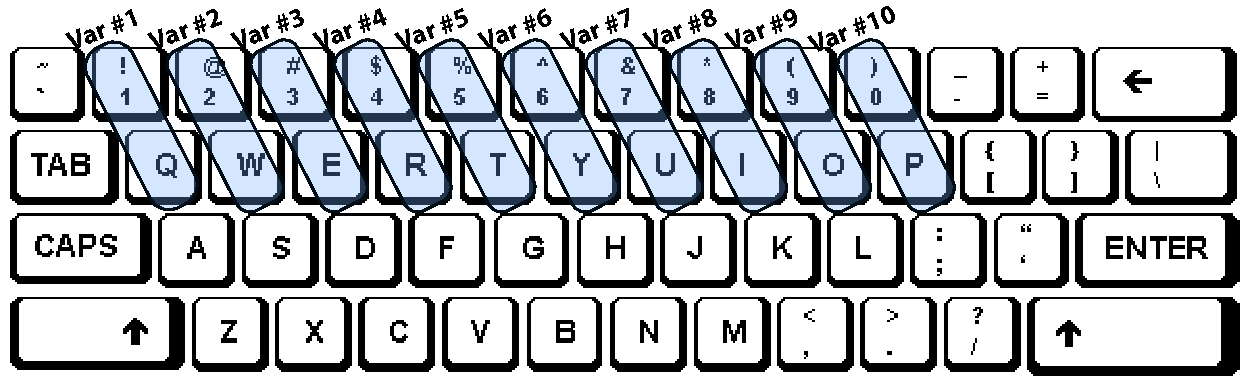
\includegraphics[width=5in]{keyboard.pdf}
  \caption[Bindings of key pairs on the keyboard to variables.]
{Ten pairs of keys on the keyboard are bound to ten variables so that pressing a key of a given pair
will either increment or decrement the associated variable. The first key pair bound to variable
number 1 are the \vn{1} and \vn{Q} keys, etc.}
  \label{f:keyboard}
\end{figure}

%% key_table ------------------------------------------------------------------------
\section{Key Bindings}\index{key bindings}
\label{s:key.bind}

\begin{figure}
  \centering
  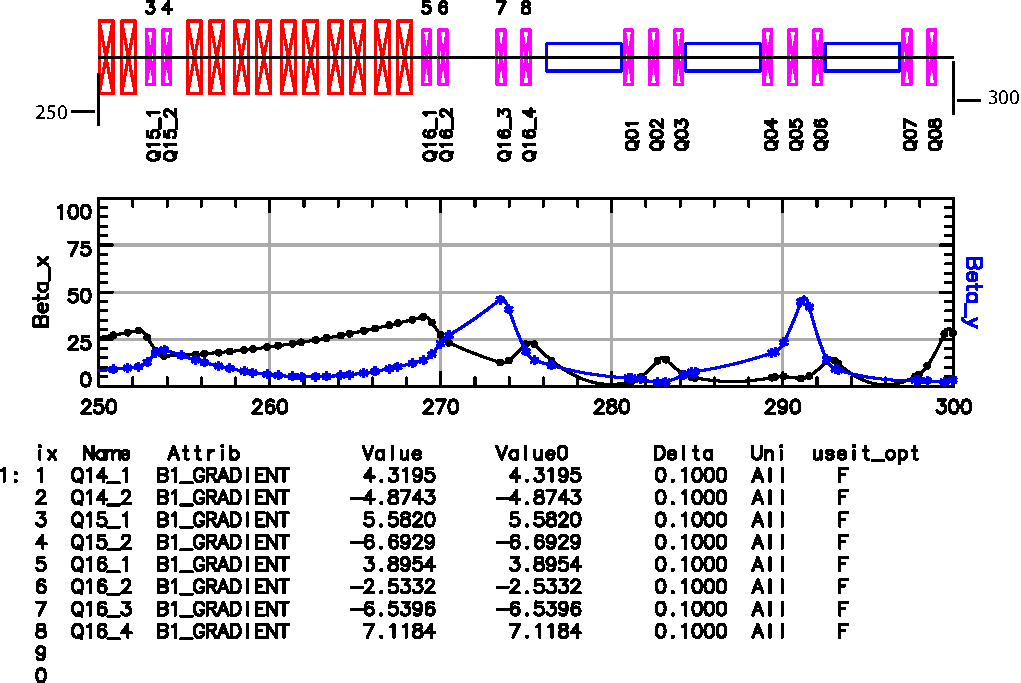
\includegraphics[width=5in]{layout-graph-table.pdf}
  \caption[Example key table with a lattice layout and data plots.]
{A lattice layout plot (top) above a data plot (middle) which in turn is above a key table plot
(bottom). Elements that have attributes that are varied as shown in the key table have the
corresponding key table number printed above the element's glyph in the lattice layout.}
  \label{f:key.table}
\end{figure}

\index{key bindings}
The main purpose of Single Mode is to associate certain keyboard keys with certain variables so that
the pressing of these keys will change their associated model value of the variable as illustrated
in Figure~\ref{f:keyboard}. This is called a \vn{key binding}. Key bindings are established in a
startup file by setting the \vn{var(i)%key_bound} and \vn{var(i)%key_delta} parameters (see
Section~\sref{s:init.var}). After startup, associated variables with keyboard keys can be done using
the \vn{set variable} command (\sref{s:set}).

The variables are divided into banks of 10. The 0\Th bank uses the first ten variables that have
their \vn{key_bound} attribute (\sref{s:init.var}) set to True.  the 1\St bank uses the next ten,
etc.  At any one time, only one bank is active. To see the status of this bank, a \vn{key_table}
plot (\sref{s:key.table})can be setup as shown in Figure~\ref{f:key.table}. The relationship between
the keys and a change in a variable is:
\begin{example}
                 Change by factor of:          
     Variable    -10  -1    1     10
   ----------    ---  ---  ---  -------
    1 + 10*ib     Q    q    1   shift-1   ("!")
    2 + 10*ib     W    w    2   shift-2   ("@")
    3 + 10*ib     E    e    3   shift-3   ("\#")
    4 + 10*ib     R    r    4   shift-4   ("\$")
    5 + 10*ib     T    t    5   shift-5   ("%")
    6 + 10*ib     Y    y    6   shift-6   ("^")
    7 + 10*ib     U    u    7   shift-7   ("\&")
    8 + 10*ib     I    i    8   shift-8   ("*")
    9 + 10*ib     O    o    9   shift-9   ("(")
   10 + 10*ib     P    p    0   shift-0   (")")
\end{example}
In the above table ib is the bank number (0 for the
0\Th bank, etc.), and the change is in multiples of the \vn{step} (\sref{s:init.var}).  value for a
variable. Note: In \vn{line mode}, the command \vn{show key_bindings} (\sref{s:show}) may be used to
show the entire set of bound keys.

Initially the 0\Th bank is active. The left arrow and right arrow are used to decrease or increase
the bank number.  Additionally the "\vn{<}" and "$>$" keys can be used to change the deltas for the
variables.

For example, looking at Figure~\ref{f:key.table}, the \vn{"1:"} in the upper left corner of the
\vn{Key Table} shows that the 1\St bank is active. \vn{key(14)} is associated with the \vn{"4"} key
and from the \vn{Key Table} it is seen that the bound attribute is the \vn{b1_gradient} of the
element named \vn{Q15_2}.  Thus, if the \vn{"4"} key is depressed in single mode, the value of the
\vn{b1_gradient} of element \vn{Q15_2} will be increased by the given Delta (0.1000 in this
case). Pressing the \vn{"r"} key (which is just below the \vn{"4"} key) will decrease the value of
the \vn{b1_gradient} by 0.1000. Using the shift key, which is shift-4 (\vn{"\$"}) will increase
\vn{b1_gradient} by 10 times the given delta (1.000 in this case) and \vn{"R"} will decrease, by a
factor of 10, the given delta.

Since element \vn{Q15_2} is also displayed in the \vn{Lattice Layout}, there is a \vn{"4"} drawn
above this element that reflects the fact that the element contains a bound attribute. Since, in
this case, the Lattice Layout only shows part of the lattice, not all key indexes are present.

%------------------------------------------------------------------------

%% keys ------------------------------------------------------------------------
\section{List of Key Strokes}\index{single mode!list of Key strokes}
\label{s:keys}

In the following list, certain commands use multiple key strokes. For example, the \vn{"/v"} command
is invoked by first pressing the slash (\vn{"/"}) key followed by the \vn{"v"} key. \vn{"a
$<$left_arrow$>$"} represents pressing the \vn{"a"} key followed by the left-arrow key.

Additionally, custom commands can be associated with any key using the \vn{set key} command
\sref{s:set}. Example:
\begin{example}
  set key h = veto var *  ! This sets the "h" key to the command "veto var *"
\end{example}

\begin{description}
\item[?]
Type a short help message.

\item[a $<$left\_arrow$>$]
Pan plots left by half the plot width.

\item[a $<$right\_arrow$>$]
Pan plots right by half the plot width.

\item[a $<$up\_arrow$>$]
Pan plots up by half the plot height.

\item[a $<$down\_arrow$>$]
Pan plots down by half the plot height.

\item[s $<$left\_arrow$>$]
Scale x-axis of plots by a factor of 2.0.

\item[s $<$right\_arrow$>$]
Scale x-axis of plots by a factor of 0.5

\item[s $<$up\_arrow$>$]
Scale y-axis of plots by a factor of 2.0.

\item[s $<$down\_arrow$>$]
Scale y-axis of plots by a factor of 0.5


\item[z $<$left\_arrow$>$]
Zoom x-axis of plots by a factor of 2.0.

\item[z $<$right\_arrow$>$]
Zoom x-axis of plots by a factor of 0.5

\item[z $<$up\_arrow$>$]
Zoom y-axis of plots by a factor of 2.0.

\item[z $<$down\_arrow$>$]
Zoom y-axis of plots by a factor of 0.5

\item[c]  
Show constraints.

\item[g]
Go run the default optimizer (\sref{s:tao.opti}). The optimizer will run until you type a '.' (a
period).  Periodically during the optimization the variable values will be written to files, one for
each universe, whose name is \vn{tao_opt_vars\#.dat}. where \vn{\#} is the universe number.

\item[v]
Show Bmad variable values in bmad lattice format. See also the \vn{/v} command. Equivalent to
\vn{show vars -bmad} in line mode.

\item[V] 
Same an \vn{v} except only variables currently enabled for optimization are shown.
This is equivalent to \vn{show vars -bmad -good} in line mode.

\item[Z] 
Go back to \vn{line mode}

\item[$<$]
Reduce the deltas (the amount that a variable is changed when you use
the keys 0 through 9) of all the variables by a factor of 2.

\item[$>$]
Increase the deltas (the amount that a variable is changed when you
use the keys 0 through 9) of all the variables by a factor of 2.

\item[$<$left\_arrow$>$]
Shift the active key bank down by 1: ib -$>$ ib - 1

\item[$<$right\_arrow$>$]
Shift the active key bank up by 1: ib -$>$ ib + 1

\item[/$<$up\_arrow$>$]
Increase all key deltas by a factor of 10.

\item[/$<$down\_arrow$>$]
Decrease all key deltas by a factor of 10.

\item[$<$CR$>$]
Do nothing but replot.

\item[-p]
Toggle plotting. Whether to plot or not to plot is initially determined by \vn{plot%enable}.

\item['$<$command$>$]
Accept a Line Mode (\sref{c:command}) command.

\item[/b]
Switch the default lattice branch (\sref{s:lattice}).

\item[/e $<$Index or Name$>$]
Prints info on a lattice element. If there are two lattices being used and only the information of
an element from one particular lattice is wanted then prepend with "n@" where n is the lattice
index.

\item[/l]
Print a list of the lattice elements with Twiss parameters.

\item[/u $<$Universe Index$>$]
Switch the default universe (\sref{s:universe}).

\item[/v]
Write variable values to the default output file in Bmad lattice format.  The default output file
name is set by \vn{global%var_out}.  See also the \vn{V} command.

\item[/x $<$min$>$ $<$max$>$]
Set the horizontal scale min and max values for all the plots. This is the same as setting
\vn{default_graph%x%min} and \vn{default_graph%x%max} in the \tao input file. If \vn{min} and
\vn{max} are not given then the scale will be chosen to include the entire lattice.

\item[/y $<$min$>$ $<$max$>$]
Set the y-axis min and max values for all the plots. This is the same as setting \vn{plot%y%min} and
\vn{plot%y%max} in the \tao input file. If \vn{min} and \vn{max} are not given then an autoscale
will be done.

\item[=v $<$digit$>$ $<$value$>$]
Set variable value. \vn{<digit>} is between 0 and 9 corresponding to a
variable of the current bank. \vn{<value>} is the value to set the
variable to.

\item[=$<$right\_arrow$>$]
Set saved ("value0") values to variable values to saved values. The saved values (the value0 column
in the display) are initially set to the initial value on startup. There are saved values for both
the manual and automatic variables. Note that reading in a TOAD input file will reset the saved
values. If you want to save the values of the variables in this case use "/w" to save to a file. Use
the "\vn{/$<$left_arrow$>$}" command to go in the reverse direction.

\item[=$<$left\_arrow$>$]
Paste saved (\vn{value0} column in the display) values back to the variable values.  The saved
values are initially set to the initial value on startup. Use the "\vn{/$<$right_arrow$>$}" command
to go in the reverse direction.

\end{description}

\chapter{Python Interface to Tao}
\index{python interface}
\label{c:python}

It is sometimes convenient to interface \tao to a scripting language like Python or interface to
some external program.  Applications include analyzing Tao generated data or 
to interface \tao to an online control system environment.

To aid in interfacing, \tao has the \vn{pipe} command (\sref{s:pipe.cmd}).\footnote
  {
Formally this command was called \vn{python} but the name was changed to avoid confusion with
the scripting language Python.
  }
The \vn{pipe} command defaines a standardized syntax with which to communicate with \tao.

Another aid is the \vn{PyTao} package which is an interface layer to be used between \tao and
\vn{Python}. See \sref{s:pytao} for more details.

%--------------------------------------------------------------------------
\section{PyTao Interface}
\label{s:pytao}

The \vn{PyTao} package is an interface layer to be used between \tao and
\vn{Python}. \vn{PyTao} is hosted on \vn{GitHub}
(independent of \bmad distributions) at:
\vspace{-2ex}
\begin{itemize}
  \item[] \url{https://bmad-sim.github.io/pytao}
\end{itemize}
\vspace{-2ex}
Documentation for setup and using PyTao is at:
\begin{example}
  bmad-sim.github.io/pytao/
\end{example}
See the \vn{PyTao} documentation for installation instructions, examples, etc. In this chapter, some
simple examples will be given.

The \vn{PyTao} package uses \tao's \vn{pipe} command to ease integration with \vn{Python}.

There are two ways to interface with Python/PyTao. One way is using the Python \vn{ctypes}
library. The other way is using the \vn{pexpect} module. A Web search will point to documentation on
\vn{ctypes} and \vn{pexpect}. 

\vn{ctypes} is a foreign function library for Python which can be used to link to a \tao shared
library.  The \vn{pexpect} module is a general purpose tool for interfacing Python with programs
like \tao. If \vn{pexpect} is not present your system, it can be downloaded from
\vn{www.noah.org/wiki/pexpect}.

The advantage of \vn{ctypes} is that it directly accesses \tao code
which makes communication between Python and \tao more robust. The disadvantage of \vn{ctypes} is
that it needs a shared-object version of the \vn{Tao} library. [See the Bmad web site for
information on building shared-object libraries.] The disadvantage of \vn{pexpect} is that it is
slower and it is possible for \vn{pexpect} to time out waiting for a response from \tao.

%--------------------------------------------------------------------------
\subsection{Python/PyTao Via Pexpect}

For communicaiton via \vn{pexpect} (\sref{s:pytao}), the python module \vn{tao_pipe.py}, is
provided by \vn{PyTao} in the directory \vn{pytao/tao_pexpect}.

Example Python session:
\begin{example}
  >>> from pytao.tao_pexpect import tao_pipe  # import module
  >>> p = tao_pipe.tao_io("-lat my_lat.bmad") # init session
  >>> out = p.cmd_in("show global")           # Command to Tao
  >>> print(out)                              # print the output from Tao
  >>> p.cmd("show global")                    # Like p.cmd_in() excepts prints the output too.
\end{example}

%--------------------------------------------------------------------------
\subsection{Python/PyTao Interface Via Ctypes}

A \vn{ctypes} based Python module \vn{pytao.py} for interfacing \tao to \vn{Python} is provided by
\vn{PyTao} (\sref{s:pytao}) in the directory \vn{pytao/tao_pexpect}.

A test driver script named \vn{pytao_example.py} is in the same directory. See the documentation in
both of these files for further information.

%--------------------------------------------------------------------------
\section{Tao's Pipe Command}
\label{s:pipe.cmd}

\tao's \vn{pipe} (\sref{s:pipe}) command was developed to:
%
\begin{itemize}
\item 
Standardize output of information (data, parameters, etc.) from \tao to simplify the task of
interfacing \tao to external programs especially scripting languages like \vn{Python}.
% 
\item 
Act as an intermediate layer for the control of \tao by such things as machine online control
programs or the planned graphical user interface for \tao.
\end{itemize}

Using the \vn{pipe} command to control \tao will not be covered here. The interested reader is
invited to read the sections of this manual on the coding of \tao and look at the \tao code itself
(which is heavily documented).

Using the \vn{pipe} command is far superior to using the \vn{show} command when interfacing to an
external program. For one, the \vn{pipe} command is formatted for ease of parsing. Another reason
to use the \vn{pipe} command is that, as \tao is developed over time, the output format of the
\vn{pipe} command is much more stable than output from the \vn{show} command.\footnote
  {
The output of the \vn{pipe} command will change when \tao's or \bmad's internal structures are
modified. This is in contrast to the \vn{show} command whose output is formated to be human readible
and whose output format may change on a whim.
  }
Thus the risk of User developed interface code breaking is much reduced by using the \vn{pipe} command.

The general form of the \vn{pipe} command is:
\begin{example}
  pipe <subcommand> <arguments>
\end{example}
The \vn{pipe} command has a number of \vn{subcommands} (over 100) that are listed in
\Sref{s:pipe.sub}. The sub-commands can be divided into two categories. One category are the
``\vn{action}'' subcommands which allow the user to control \tao (for example, creating variables
and data for use in an optimization). The other category are the ``\vn{output}'' subcommands which
output information from \tao.

The output of the \vn{pipe} command are semi-colon delimited lists. Example: With the
\vn{pipe global} the output looks like:
\begin{example}
  lm_opt_deriv_reinit;REAL;T; -1.0000000000000000E+00
  de_lm_step_ratio;REAL;T;  1.0000000000000000E+00
  de_var_to_population_factor;REAL;T;  5.0000000000000000E+00
  unstable_penalty;REAL;T;  1.0000000474974513E-03
  n_opti_cycles;INT;T;20
  track_type;ENUM;T;single
  derivative_uses_design;LOGIC;T;F
  ... etc ...
\end{example}

Most \vn{output} subcommands use ``\vn{parameter list form}'' format where each line has four fields
separated by semicolons:
\begin{example}
  {name};{type};{variable};{value(s)}
\end{example}
The fields are:
\begin{example}
    name:       The name of the parameter

    type:       The type of the parameter:
        INT           Integer number
        REAL          Real number
        COMPLEX       Complex number. A complex number is output as Re;Im
        REAL_ARR      Real array
        LOGIC         Logical: "T" or "F".
        INUM          Integer whose allowed values can be obtained 
                        using the "pipe inum" command.
        ENUM          String whose allowed values can be obtained 
                        using the "pipe enum" command.
        FILE          Name of file.
        CRYSTAL       Crystal name string. EG: "Si(111)"
        DAT_TYPE      Data type string. EG: "orbit.x"
        DAT_TYPE_Z    Data type string if plot%x_axis_type = 'data'. 
                        Otherwise is a data_type_z enum.
        SPECIES       Species name string. EG: "H2SO4++"
        ELE_PARAM     Lattice element parameter string. EG "K1"
        STR           String that does not fall into one of the above string categories.
        STRUCT        Structure. In this case {component_value(s)} is of the form:
                        {name1};{type1};{value1};{name2};{type2};{value2};...
        COMPONENT     For curve component parameters.

    can_vary:   Either 'T', 'F', or 'I', indicating whether or not the
                user may change the value of the parameter. 'I' indicates
                that the parameter is to be ignored by a GUI when displaying parameters.

    value(s):   The value or values of the the parameter. If a parameter has multiple
                values (EG an array), the values will be separated by semicolons.
\end{example}

%--------------------------------------------------------------------------
\section{Plotting Issues}
\label{s:gui.plot}

When using \tao with a \vn{GUI}, and when the \vn{GUI} is doing the plotting, the \vn{-noplot} and
\vn{-external_plotting} options (\sref{s:command.line}) should be used when starting \tao. The
\vn{-noplot} option (which sets \vn{global%plot_on}) prevents \tao from opening a plotting
window. Note: Both of these options can also be set, after startup, with the \vn{set global} command
and the setting of both can be viewed using the \vn{show global} command.

With \vn{-external_plotting} set, the external code should handle how plots are assigned to plot
regions and it would be potentially disruptive if a user tired to place plots (which could
inadvertently happen when running command files). To avoid this, with \vn{-external_plotting} set,
the \vn{place} command will not do any placement but rather save the \vn{place} arguments (which is
the name of a template plot and a region name) to a buffer which then can be read out by the
external code using the \vn{pipe place_buffer} command. The external code may then decide how to
proceed. The external code is able to bypass the buffering and perform placements by using
\vn{place} with the \vn{-no_buffer} switch (\sref{s:place}). Notice: \tao never processes place
command information put in the buffer. It is up to the external code to decide on a course of action.

Normally when \tao is not displaying the plot page when the \vn{-noplot} option is used, \tao will,
to save time, not calculate the points needed for plotting curves. The exception is if
\vn{-external_plotting} is turned on. In this case, to make plot references unambiguous, a plot can be
referred to by its index number. The plot index number can be viewed using the \vn{pipe
plot_list} command. Template plots can be referenced using the syntax ``\vn{@Tnnn}'' where \vn{nnn}
is the index number. For example, \vn{@T3} referrers to the template plot with index 3. Similarly,
the displayed plots (plots that are associated with plot regions) can be referred to using the
syntax ``\vn{@Rnnn}''.

%--------------------------------------------------------------------------
\section{Pipe subcommands}
\label{s:pipe.sub}

The \vn{pipe} command has the following subcommands:

% WARNING: this is automatically generated. DO NOT EDIT.

%% pipe beam ------------------------------------
\subsection{pipe beam}
\index{pipe!beam}
\label{p:beam}


Output beam parameters that are not in the beam_init structure.

\begin{example}
   pipe beam \{ix_uni\}@\{ix_branch\}
\end{example}
\begin{verbatim}
Where:
  {ix_uni} is a universe index. Defaults to s%global%default_universe.
  {ix_branch} is a lattice branch index. Defaults to s%global%default_branch.

Note: To set beam_init parameters use the "set beam" command.
\end{verbatim}

%% pipe beam_init ------------------------------------
\subsection{pipe beam_init}
\index{pipe!beam_init}
\label{p:beam.init}


Output beam_init parameters.

\begin{example}
   pipe beam_init \{ix_uni\}@\{ix_branch\}
\end{example}
\begin{verbatim}
Where:
  {ix_uni} is a universe index. Defaults to s%global%default_universe.
  {ix_branch} is a lattice branch index. Defaults to s%global%default_branch.

Note: To set beam_init parameters use the "set beam_init" command
\end{verbatim}

%% pipe bmad_com ------------------------------------
\subsection{pipe bmad_com}
\index{pipe!bmad_com}
\label{p:bmad.com}


Output bmad_com structure components.

\begin{example}
   pipe bmad_com
\end{example}
\begin{verbatim}

\end{verbatim}

%% pipe branch1 ------------------------------------
\subsection{pipe branch1}
\index{pipe!branch1}
\label{p:branch1}


Output lattice branch information for a particular lattice branch.

\begin{example}
   pipe branch1 \{ix_uni\}@\{ix_branch\}
\end{example}
\begin{verbatim}
Where:
  {ix_uni} is a universe index. Defaults to s%global%default_universe.
  {ix_branch} is a lattice branch index. Defaults to s%global%default_branch.
\end{verbatim}

%% pipe bunch_comb ------------------------------------
\subsection{pipe bunch_comb}
\index{pipe!bunch_comb}
\label{p:bunch.comb}


Outputs bunch parameters at a comb point. 
Also see the "write bunch_comb" and "show bunch -comb" commands.

\begin{example}
   pipe bunch_comb \{flags\} \{who\} \{ix_uni\}@\{ix_branch\} \{ix_bunch\}
\end{example}
\begin{verbatim}
Where:
  {flags} are optional switches:
      -array_out : If present, the output will be available in the 
             tao_c_interface_com%c_real array.
  {ix_uni} is a universe index. Defaults to s%global%default_universe.
  {ix_branch} is a branch index. Defaults to s%global%default_branch.
  {ix_bunch} is the bunch index. Defaults to 1.
  {who} is one of:
      x, px, y, py, z, pz, t, s, spin.x, spin.y, spin.z, p0c, beta     -- centroid 
      x.Q, y.Q, z.Q, a.Q, b.Q, c.Q where Q is one of: beta, alpha, gamma, phi, 
                                      eta, etap, sigma, sigma_p, emit, norm_emit
    sigma.IJ where I, J in range [1,6]
    rel_min.I, rel_max.I where I in range [1,6]
    charge_live, n_particle_live, n_particle_lost_in_ele, ix_ele

  Note: If ix_uni or ix_branch is present, "@" must be present.

Example:
  pipe bunch_comb py 2@1 1
\end{verbatim}

%% pipe bunch_params ------------------------------------
\subsection{pipe bunch_params}
\index{pipe!bunch_params}
\label{p:bunch.params}


Outputs bunch parameters at the exit end of a given lattice element.

\begin{example}
   pipe bunch_params \{ele_id\}|\{which\}
\end{example}
\begin{verbatim}
Where:
  {ele_id} is an element name or index.
  {which} is one of: "model", "base" or "design"

Example:
  pipe bunch_params end|model  ! parameters at model lattice element named "end".
\end{verbatim}

%% pipe bunch1 ------------------------------------
\subsection{pipe bunch1}
\index{pipe!bunch1}
\label{p:bunch1}


Outputs Bunch parameters at the exit end of a given lattice element.

\begin{example}
   pipe bunch1 \{ele_id\}|\{which\} \{ix_bunch\} \{coordinate\}
\end{example}
\begin{verbatim}
Where:
  {ele_id} is an element name or index.
  {which} is one of: "model", "base" or "design"
  {ix_bunch} is the bunch index.
  {coordinate} is one of: x, px, y, py, z, pz, "s", "t", "charge", "p0c", 
                                                                "state", "ix_ele"

For example, if {coordinate} = "px", the phase space px coordinate of each particle
of the bunch is displayed. The "state" of a particle is an integer. 
A value of 1 means alive and any other value means the particle has been lost.
\end{verbatim}

%% pipe building_wall_list ------------------------------------
\subsection{pipe building_wall_list}
\index{pipe!building_wall_list}
\label{p:building.wall.list}


Output List of building wall sections or section points

\begin{example}
   pipe building_wall_list \{ix_section\}
\end{example}
\begin{verbatim}
Where:
  {ix_section} is a building wall section index.

If {ix_section} is not present, a list of building wall sections is given.
If {ix_section} is present, a list of section points is given.
\end{verbatim}

%% pipe building_wall_graph ------------------------------------
\subsection{pipe building_wall_graph}
\index{pipe!building_wall_graph}
\label{p:building.wall.graph}


Output (x, y) points for drawing the building wall for a particular graph.

\begin{example}
   pipe building_wall_graph \{graph\}
\end{example}
\begin{verbatim}
Where:
  {graph} is a plot region graph name.

Note: The graph defines the coordinate system for the (x, y) points.
\end{verbatim}

%% pipe building_wall_point ------------------------------------
\subsection{pipe building_wall_point}
\index{pipe!building_wall_point}
\label{p:building.wall.point}


add or delete a building wall point

\begin{example}
   pipe building_wall_point \{ix_section\}^^\{ix_point\}^^\{z\}^^\{x\}^^\{radius\}^^
                                                               \{z_center\}^^\{x_center\}
\end{example}
\begin{verbatim}
Where:
  {ix_section}    -- Section index.
  {ix_point}      -- Point index. Points of higher indexes will be moved up 
                       if adding a point and down if deleting.
  {z}, etc...     -- See tao_building_wall_point_struct components.
                  -- If {z} is set to "delete" then delete the point.
\end{verbatim}

%% pipe building_wall_section ------------------------------------
\subsection{pipe building_wall_section}
\index{pipe!building_wall_section}
\label{p:building.wall.section}


Add or delete a building wall section

\begin{example}
   pipe building_wall_section \{ix_section\}^^\{sec_name\}^^\{sec_constraint\}
\end{example}
\begin{verbatim}
Where:
  {ix_section}      -- Section index. Sections with higher indexes will be
                         moved up if adding a section and down if deleting.
  {sec_name}        -- Section name.
  {sec_constraint}  -- A section constraint name or "delete". Must be one of:
      delete          -- Delete section. Anything else will add the section.
      none
      left_side
      right_side
\end{verbatim}

%% pipe constraints ------------------------------------
\subsection{pipe constraints}
\index{pipe!constraints}
\label{p:constraints}


Output optimization data and variable parameters that contribute to the merit function.

\begin{example}
   pipe constraints \{who\}
\end{example}
\begin{verbatim}
Where:
  {who} is one of: "data" or "var"

Data constraints output is:
  data name
  constraint type
  evaluation element name
  start element name
  end/reference element name
  measured value
  ref value (only relavent if global%opt_with_ref = T)
  model value
  base value (only relavent if global%opt_with_base = T)
  weight
  merit value
  location where merit is evaluated (if there is a range)
Var constraints output is:
  var name
  Associated varible attribute
  meas value
  ref value (only relavent if global%opt_with_ref = T)
  model value
  base value (only relavent if global%opt_with_base = T)
  weight
  merit value
  dmerit/dvar
\end{verbatim}

%% pipe da_aperture ------------------------------------
\subsection{pipe da_aperture}
\index{pipe!da_aperture}
\label{p:da.aperture}


Output dynamic aperture data

\begin{example}
   pipe da_aperture \{ix_uni\}
\end{example}
\begin{verbatim}
Where:
  {ix_uni} is a universe index. Defaults to s%global%default_universe.
\end{verbatim}

%% pipe da_params ------------------------------------
\subsection{pipe da_params}
\index{pipe!da_params}
\label{p:da.params}


Output dynamic aperture input parameters

\begin{example}
   pipe da_params \{ix_uni\}
\end{example}
\begin{verbatim}
Where:
  {ix_uni} is a universe index. Defaults to s%global%default_universe.
\end{verbatim}

%% pipe data ------------------------------------
\subsection{pipe data}
\index{pipe!data}
\label{p:data}


Output Individual datum parameters.

\begin{example}
   pipe data \{ix_uni\}@\{d2_name\}.\{d1_name\}[\{dat_index\}]
\end{example}
\begin{verbatim}
Where:
  {ix_uni} is a universe index. Defaults to s%global%default_universe.
  {d2_name} is the name of the d2_data structure the datum is in.
  {d1_datum} is the name of the d1_data structure the datum is in.
  {dat_index} is the index of the datum.

Use the "pipe data-d1" command to get detailed info on a specific d1 array.

Example:
  pipe data 1@orbit.x[10]
\end{verbatim}

%% pipe data_d_array ------------------------------------
\subsection{pipe data_d_array}
\index{pipe!data_d_array}
\label{p:data.d.array}


Output list of datums for a given d1_data structure.

\begin{example}
   pipe data_d_array \{ix_uni\}@\{d2_name\}.\{d1_name\}
\end{example}
\begin{verbatim}
Where:
  {ix_uni} is a universe index. Defaults to s%global%default_universe.
  {d2_name} is the name of the containing d2_data structure.
  {d1_name} is the name of the d1_data structure containing the array of datums.

Example:
  pipe data_d_array 1@orbit.x
\end{verbatim}

%% pipe data_d1_array ------------------------------------
\subsection{pipe data_d1_array}
\index{pipe!data_d1_array}
\label{p:data.d1.array}


Output list of d1 arrays for a given data_d2.

\begin{example}
   pipe data_d1_array \{d2_datum\}
\end{example}
\begin{verbatim}
{d2_datum} should be of the form
  {ix_uni}@{d2_datum_name}
\end{verbatim}

%% pipe data_d2 ------------------------------------
\subsection{pipe data_d2}
\index{pipe!data_d2}
\label{p:data.d2}


Output information on a d2_datum.

\begin{example}
   pipe data_d2 \{ix_uni\}@\{d2_name\}
\end{example}
\begin{verbatim}
Where:
  {ix_uni} is a universe index. Defaults to s%global%default_universe.
  {d2_name} is the name of the d2_data structure.
\end{verbatim}

%% pipe data_d2_array ------------------------------------
\subsection{pipe data_d2_array}
\index{pipe!data_d2_array}
\label{p:data.d2.array}


Output data d2 info for a given universe.

\begin{example}
   pipe data_d2_array \{ix_uni\}
\end{example}
\begin{verbatim}
Where:
  {ix_uni} is a universe index. Defaults to s%global%default_universe.

Example:
  pipe data_d2_array 1
\end{verbatim}

%% pipe data_d2_create ------------------------------------
\subsection{pipe data_d2_create}
\index{pipe!data_d2_create}
\label{p:data.d2.create}


Create a d2 data structure along with associated d1 and data arrays.

\begin{example}
   pipe data_d2_create \{ix_uni\}@\{d2_name\}^^\{n_d1_data\}^^\{d_data_arrays_name_min_max\}
\end{example}
\begin{verbatim}
Where:
  {ix_uni} is a universe index. Defaults to s%global%default_universe.
  {d2_name} is the name of the d2_data structure to create.
  {n_d1_data} is the number of associated d1 data structures.
  {d_data_arrays_name_min_max} has the form
    {name1}^^{lower_bound1}^^{upper_bound1}^^....
                                           ^^{nameN}^^{lower_boundN}^^{upper_boundN}
  where {name} is the data array name and 
  {lower_bound} and {upper_bound} are the bounds of the array.

Example:
  pipe data_d2_create 2@orbit^^2^^x^^0^^45^^y^^1^^47
This example creates a d2 data structure called "orbit" with 
two d1 structures called "x" and "y".

The "x" d1 structure has an associated data array with indexes in the range [0, 45].
The "y" d1 structure has an associated data arrray with indexes in the range [1, 47].

Use the "set data" command to set created datum parameters.

Note: When setting multiple data parameters, 
      temporarily toggle s%global%lattice_calc_on to False
  ("set global lattice_calc_on = F") to prevent Tao trying to 
      evaluate the partially created datum and generating unwanted error messages.
\end{verbatim}

%% pipe data_d2_destroy ------------------------------------
\subsection{pipe data_d2_destroy}
\index{pipe!data_d2_destroy}
\label{p:data.d2.destroy}


Destroy a d2 data structure along with associated d1 and data arrays.

\begin{example}
   pipe data_d2_destroy \{ix_uni\}@\{d2_name\}
\end{example}
\begin{verbatim}
Where:
  {ix_uni} is a universe index. Defaults to s%global%default_universe.
  {d2_name} is the name of the d2_data structure to destroy.

Example:
  pipe data_d2_destroy 2@orbit
This destroys the orbit d2_data structure in universe 2.
\end{verbatim}

%% pipe data_parameter ------------------------------------
\subsection{pipe data_parameter}
\index{pipe!data_parameter}
\label{p:data.parameter}


Output an array of values for a particular datum parameter for a given array of datums, 

\begin{example}
   pipe data_parameter \{data_array\} \{parameter\}
\end{example}
\begin{verbatim}
{parameter} may be any tao_data_struct parameter.
Example:
  pipe data_parameter orbit.x model_value
\end{verbatim}

%% pipe data_set_design_value ------------------------------------
\subsection{pipe data_set_design_value}
\index{pipe!data_set_design_value}
\label{p:data.set.design.value}


Set the design (and base \& model) values for all datums.

\begin{example}
   pipe data_set_design_value
\end{example}
\begin{verbatim}
Example:
  pipe data_set_design_value

Note: Use the "data_d2_create" and "datum_create" first to create datums.
\end{verbatim}

%% pipe datum_create ------------------------------------
\subsection{pipe datum_create}
\index{pipe!datum_create}
\label{p:datum.create}


Create a datum.

\begin{example}
   pipe datum_create \{datum_name\}^^\{data_type\}^^\{ele_ref_name\}^^\{ele_start_name\}^^
                       \{ele_name\}^^\{merit_type\}^^\{meas\}^^\{good_meas\}^^\{ref\}^^
                       \{good_ref\}^^\{weight\}^^\{good_user\}^^\{data_source\}^^
                       \{eval_point\}^^\{s_offset\}^^\{ix_bunch\}^^\{invalid_value\}^^
                       \{spin_axis%n0(1)\}^^\{spin_axis%n0(2)\}^^\{spin_axis%n0(3)\}^^
                       \{spin_axis%l(1)\}^^\{spin_axis%l(2)\}^^\{spin_axis%l(3)\}
\end{example}
\begin{verbatim}
Note: The 3 values for spin_axis%n0, as a group, are optional. 
      Also the 3 values for spin_axis%l are, as a group, optional.
Note: Use the "pipe data_d2_create" command first to create a d2 structure 
      with associated d1 arrays.
Note: After creating all your datums, use the "pipe data_set_design_value" routine
      to set the design (and model) values.
\end{verbatim}

%% pipe datum_has_ele ------------------------------------
\subsection{pipe datum_has_ele}
\index{pipe!datum_has_ele}
\label{p:datum.has.ele}


Output whether a datum type has an associated lattice element

\begin{example}
   pipe datum_has_ele \{datum_type\}
\end{example}
\begin{verbatim}

\end{verbatim}

%% pipe derivative ------------------------------------
\subsection{pipe derivative}
\index{pipe!derivative}
\label{p:derivative}


Output optimization derivatives

\begin{example}
   pipe derivative
\end{example}
\begin{verbatim}
Note: To save time, this command will not recalculate derivatives. 
Use the "derivative" command beforehand to recalcuate if needed.
\end{verbatim}

%% pipe ele:ac_kicker ------------------------------------
\subsection{pipe ele:ac_kicker}
\index{pipe!ele:ac_kicker}
\label{p:ele:ac.kicker}


Output element ac_kicker parameters

\begin{example}
   pipe ele:ac_kicker \{ele_id\}|\{which\}
\end{example}
\begin{verbatim}
Where: 
  {ele_id} is an element name or index.
  {which} is one of: "model", "base" or "design"

Example:
  pipe ele:ac_kicker 3@1>>7|model
This gives element number 7 in branch 1 of universe 3.
\end{verbatim}

%% pipe ele:cartesian_map ------------------------------------
\subsection{pipe ele:cartesian_map}
\index{pipe!ele:cartesian_map}
\label{p:ele:cartesian.map}


Output element cartesian_map parameters

\begin{example}
   pipe ele:cartesian_map \{ele_id\}|\{which\} \{index\} \{who\}
\end{example}
\begin{verbatim}
Where:
  {ele_id} is an element name or index
  {which} is one of: "model", "base" or "design"
  {index} is the index number in the ele%cartesian_map(:) array
  {who} is one of: "base", or "terms"

Example:
  pipe ele:cartesian_map 3@1>>7|model 2 base
This gives element number 7 in branch 1 of universe 3.
\end{verbatim}

%% pipe ele:chamber_wall ------------------------------------
\subsection{pipe ele:chamber_wall}
\index{pipe!ele:chamber_wall}
\label{p:ele:chamber.wall}


Output element beam chamber wall parameters

\begin{example}
   pipe ele:chamber_wall \{ele_id\}|\{which\} \{index\} \{who\}
\end{example}
\begin{verbatim}
Where:
  {ele_id} is an element name or index.
  {which} is one of: "model", "base" or "design"
  {index} is index of the wall.
  {who} is one of:
    "x"       ! Return min/max in horizontal plane
    "y"       ! Return min/max in vertical plane
\end{verbatim}

%% pipe ele:control_var ------------------------------------
\subsection{pipe ele:control_var}
\index{pipe!ele:control_var}
\label{p:ele:control.var}


Output list of element control variables.
Used for group, overlay and ramper type elements.

\begin{example}
   pipe ele:control_var \{ele_id\}|\{which\}
\end{example}
\begin{verbatim}
Where:
  {ele_id} is an element name or index.
  {which} is one of: "model", "base" or "design"

Example:
  pipe ele:control_var 3@1>>7|model
This gives control info on element number 7 in branch 1 of universe 3.
\end{verbatim}

%% pipe ele:cylindrical_map ------------------------------------
\subsection{pipe ele:cylindrical_map}
\index{pipe!ele:cylindrical_map}
\label{p:ele:cylindrical.map}


Output element cylindrical_map

\begin{example}
   pipe ele:cylindrical_map \{ele_id\}|\{which\} \{index\} \{who\}
\end{example}
\begin{verbatim}
Where 
  {ele_id} is an element name or index.
  {which} is one of: "model", "base" or "design"
  {index} is the index number in the ele%cylindrical_map(:) array
  {who} is one of: "base", or "terms"

Example:
  pipe ele:cylindrical_map 3@1>>7|model 2 base
This gives map #2 of element number 7 in branch 1 of universe 3.
\end{verbatim}

%% pipe ele:elec_multipoles ------------------------------------
\subsection{pipe ele:elec_multipoles}
\index{pipe!ele:elec_multipoles}
\label{p:ele:elec.multipoles}


Output element electric multipoles

\begin{example}
   pipe ele:elec_multipoles \{ele_id\}|\{which\}
\end{example}
\begin{verbatim}
Where:
  {ele_id} is an element name or index.
  {which} is one of: "model", "base" or "design"

Example:
  pipe ele:elec_multipoles 3@1>>7|model
This gives element number 7 in branch 1 of universe 3.
\end{verbatim}

%% pipe ele:floor ------------------------------------
\subsection{pipe ele:floor}
\index{pipe!ele:floor}
\label{p:ele:floor}


Output element floor coordinates. The output gives four lines. "Reference" is
without element misalignments and "Actual" is with misalignments. The lines with "-W"
give the W matrix. The exception is that if ele is a multipass_lord, there will be 4*N
lines where N is the number of slaves.

\begin{example}
   pipe ele:floor \{ele_id\}|\{which\} \{where\}
\end{example}
\begin{verbatim}
Where:
  {ele_id} is an element name or index.
  {which} is one of: "model", "base" or "design"
  {where} is an optional argument which, if present, is one of
    beginning  ! Upstream end.
    center     ! Middle of the element. This is the surface of element when used 
               !  with photonic reflecting elements such as crystal and mirror elements.
    end        ! Downstream end (default).

Example:
  pipe ele:floor 3@1>>7|model
This gives element number 7 in branch 1 of universe 3.
\end{verbatim}

%% pipe ele:gen_attribs ------------------------------------
\subsection{pipe ele:gen_attribs}
\index{pipe!ele:gen_attribs}
\label{p:ele:gen.attribs}


Output element general attributes

\begin{example}
   pipe ele:gen_attribs \{ele_id\}|\{which\}
\end{example}
\begin{verbatim}
Where: 
  {ele_id} is an element name or index.
  {which} is one of: "model", "base" or "design"

Example:
  pipe ele:gen_attribs 3@1>>7|model
This gives element number 7 in branch 1 of universe 3.
\end{verbatim}

%% pipe ele:gen_grad_map ------------------------------------
\subsection{pipe ele:gen_grad_map}
\index{pipe!ele:gen_grad_map}
\label{p:ele:gen.grad.map}


Output element gen_grad_map 

\begin{example}
   pipe ele:gen_grad_map \{ele_id\}|\{which\} \{index\} \{who\}
\end{example}
\begin{verbatim}
Where: 
  {ele_id} is an element name or index.
  {which} is one of: "model", "base" or "design"
  {index} is the index number in the ele%gen_grad_map(:) array
  {who} is one of: "base", or "derivs".

Example:
  pipe ele:gen_grad_map 3@1>>7|model 2 base
This gives element number 7 in branch 1 of universe 3.
\end{verbatim}

%% pipe ele:grid_field ------------------------------------
\subsection{pipe ele:grid_field}
\index{pipe!ele:grid_field}
\label{p:ele:grid.field}


Output element grid_field

\begin{example}
   pipe ele:grid_field \{ele_id\}|\{which\} \{index\} \{who\}
\end{example}
\begin{verbatim}
Where:
  {ele_id} is an element name or index.
  {which} is one of: "model", "base" or "design"
  {index} is the index number in the ele%grid_field(:) array.
  {who} is one of: "base", or "points"

Example:
  pipe ele:grid_field 3@1>>7|model 2 base
This gives grid #2 of element number 7 in branch 1 of universe 3.
\end{verbatim}

%% pipe ele:head ------------------------------------
\subsection{pipe ele:head}
\index{pipe!ele:head}
\label{p:ele:head}


Output "head" Element attributes

\begin{example}
   pipe ele:head \{ele_id\}|\{which\}
\end{example}
\begin{verbatim}
Where: 
  {ele_id} is an element name or index.
  {which} is one of: "model", "base" or "design"

Example:
  pipe ele:head 3@1>>7|model
This gives element number 7 in branch 1 of universe 3.
\end{verbatim}

%% pipe ele:lord_slave ------------------------------------
\subsection{pipe ele:lord_slave}
\index{pipe!ele:lord_slave}
\label{p:ele:lord.slave}


Output the lord/slave tree of an element.

\begin{example}
   pipe ele:lord_slave \{ele_id\}|\{which\}
\end{example}
\begin{verbatim}
Where: 
  {ele_id} is an element name or index.
  {which} is one of: "model", "base" or "design"

Example:
  pipe ele:lord_slave 3@1>>7|model
This gives lord and slave info on element number 7 in branch 1 of universe 3.
Note: The lord/slave info is independent of the setting of {which}.

The output is a number of lines.
Each line gives information on an element (element index, etc.).
Some lines begin with the word "Element". 
After each "Element" line, there are a number of lines (possibly zero) 
that begin with the word "Slave or "Lord".
These "Slave" and "Lord" lines are the slaves and lords of the "Element" element.
\end{verbatim}

%% pipe ele:mat6 ------------------------------------
\subsection{pipe ele:mat6}
\index{pipe!ele:mat6}
\label{p:ele:mat6}


Output element mat6

\begin{example}
   pipe ele:mat6 \{ele_id\}|\{which\} \{who\}
\end{example}
\begin{verbatim}
Where: 
  {ele_id} is an element name or index.
  {which} is one of: "model", "base" or "design"
  {who} is one of: "mat6", "vec0", or "err"

Example:
  pipe ele:mat6 3@1>>7|model mat6
This gives element number 7 in branch 1 of universe 3.
\end{verbatim}

%% pipe ele:methods ------------------------------------
\subsection{pipe ele:methods}
\index{pipe!ele:methods}
\label{p:ele:methods}


Output element methods

\begin{example}
   pipe ele:methods \{ele_id\}|\{which\}
\end{example}
\begin{verbatim}
Where: 
  {ele_id} is an element name or index.
  {which} is one of: "model", "base" or "design"

Example:
  pipe ele:methods 3@1>>7|model
This gives element number 7 in branch 1 of universe 3.
\end{verbatim}

%% pipe ele:multipoles ------------------------------------
\subsection{pipe ele:multipoles}
\index{pipe!ele:multipoles}
\label{p:ele:multipoles}


Output element multipoles

\begin{example}
   pipe ele:multipoles \{ele_id\}|\{which\}
\end{example}
\begin{verbatim}
Where: 
  {ele_id} is an element name or index.
  {which} is one of: "model", "base" or "design"

Example:
  pipe ele:multipoles 3@1>>7|model
This gives element number 7 in branch 1 of universe 3.
\end{verbatim}

%% pipe ele:orbit ------------------------------------
\subsection{pipe ele:orbit}
\index{pipe!ele:orbit}
\label{p:ele:orbit}


Output element orbit

\begin{example}
   pipe ele:orbit \{ele_id\}|\{which\}
\end{example}
\begin{verbatim}
Where: 
  {ele_id} is an element name or index.
  {which} is one of: "model", "base" or "design"

Example:
  pipe ele:orbit 3@1>>7|model
This gives element number 7 in branch 1 of universe 3.
\end{verbatim}

%% pipe ele:param ------------------------------------
\subsection{pipe ele:param}
\index{pipe!ele:param}
\label{p:ele:param}


Output lattice element parameter

\begin{example}
   pipe ele:param \{ele_id\}|\{which\} \{who\}
\end{example}
\begin{verbatim}
Where: 
  {ele_id} is an element name or index.
  {which} is one of: "model", "base" or "design"
  {who} values are the same as {who} values for "pipe lat_list".
        Note: Here {who} must be a single parameter and not a list.

Example:
  pipe ele:param 3@1>>7|model e_tot
This gives E_tot of element number 7 in branch 1 of universe 3.

Note: On output the {variable} component will always be "F" (since this 
command cannot tell if a parameter is allowed to vary).

Also see: "pipe lat_list".
\end{verbatim}

%% pipe ele:photon ------------------------------------
\subsection{pipe ele:photon}
\index{pipe!ele:photon}
\label{p:ele:photon}


Output element photon parameters

\begin{example}
   pipe ele:photon \{ele_id\}|\{which\} \{who\}
\end{example}
\begin{verbatim}
Where: 
  {ele_id} is an element name or index.
  {which} is one of: "model", "base" or "design"
  {who} is one of: "base", "material", or "curvature"

Example:
  pipe ele:photon 3@1>>7|model base
This gives element number 7 in branch 1 of universe 3.
\end{verbatim}

%% pipe ele:spin_taylor ------------------------------------
\subsection{pipe ele:spin_taylor}
\index{pipe!ele:spin_taylor}
\label{p:ele:spin.taylor}


Output element spin_taylor parameters

\begin{example}
   pipe ele:spin_taylor \{ele_id\}|\{which\}
\end{example}
\begin{verbatim}
Where: 
  {ele_id} is an element name or index.
  {which} is one of: "model", "base" or "design"

Example:
  pipe ele:spin_taylor 3@1>>7|model
This gives element number 7 in branch 1 of universe 3.
\end{verbatim}

%% pipe ele:taylor ------------------------------------
\subsection{pipe ele:taylor}
\index{pipe!ele:taylor}
\label{p:ele:taylor}


Output element taylor map 

\begin{example}
   pipe ele:taylor \{ele_id\}|\{which\}
\end{example}
\begin{verbatim}
Where: 
  {ele_id} is an element name or index.
  {which} is one of: "model", "base" or "design"

Example:
  pipe ele:taylor 3@1>>7|model
This gives element number 7 in branch 1 of universe 3.
\end{verbatim}

%% pipe ele:twiss ------------------------------------
\subsection{pipe ele:twiss}
\index{pipe!ele:twiss}
\label{p:ele:twiss}


Output element Twiss parameters

\begin{example}
   pipe ele:twiss \{ele_id\}|\{which\}
\end{example}
\begin{verbatim}
Where: 
  {ele_id} is an element name or index.
  {which} is one of: "model", "base" or "design"

Example:
  pipe ele:twiss 3@1>>7|model
This gives element number 7 in branch 1 of universe 3.
\end{verbatim}

%% pipe ele:wake ------------------------------------
\subsection{pipe ele:wake}
\index{pipe!ele:wake}
\label{p:ele:wake}


Output element wake.

\begin{example}
   pipe ele:wake \{ele_id\}|\{which\} \{who\}
\end{example}
\begin{verbatim}
Where: 
  {ele_id} is an element name or index.
  {which} is one of: "model", "base" or "design"
  {Who} is one of:
      "sr_long"        "sr_long_table"
      "sr_trans"       "sr_trans_table"
      "lr_mode_table"  "base"

Example:
  pipe ele:wake 3@1>>7|model
This gives element number 7 in branch 1 of universe 3.
\end{verbatim}

%% pipe ele:wall3d ------------------------------------
\subsection{pipe ele:wall3d}
\index{pipe!ele:wall3d}
\label{p:ele:wall3d}


Output element wall3d parameters.

\begin{example}
   pipe ele:wall3d \{ele_id\}|\{which\} \{index\} \{who\}
\end{example}
\begin{verbatim}
Where: 
  {ele_id} is an element name or index.
  {which} is one of: "model", "base" or "design"
  {index} is the index number in the ele%wall3d(:) array 
            The size of this array is obtained from "pipe ele:head".
  {who} is one of: "base", or "table".
Example:
  pipe ele:wall3d 3@1>>7|model 2 base
This gives element number 7 in branch 1 of universe 3.
\end{verbatim}

%% pipe evaluate ------------------------------------
\subsection{pipe evaluate}
\index{pipe!evaluate}
\label{p:evaluate}


Output the value of an expression. The result may be a vector.

\begin{example}
   pipe evaluate \{flags\} \{expression\}
\end{example}
\begin{verbatim}
Where:
  Optional {flags} are:
      -array_out : If present, the output will be available in the 
                    tao_c_interface_com%c_real array.
  {expression} is expression to be evaluated.

Example:
  pipe evaluate 3+data::cbar.11[1:10]|model
\end{verbatim}

%% pipe em_field ------------------------------------
\subsection{pipe em_field}
\index{pipe!em_field}
\label{p:em.field}


Output EM field at a given point generated by a given element.

\begin{example}
   pipe em_field \{ele_id\}|\{which\} \{x\} \{y\} \{z\} \{t_or_z\}
\end{example}
\begin{verbatim}
Where:
  {which} is one of: "model", "base" or "design"
  {x}, {y}  -- Transverse coords.
  {z}       -- Longitudinal coord with respect to entrance end of element.
  {t_or_z}  -- time or phase space z depending if lattice is setup for 
            --   absolute time tracking.
\end{verbatim}

%% pipe enum ------------------------------------
\subsection{pipe enum}
\index{pipe!enum}
\label{p:enum}


Output list of possible values for enumerated numbers.

\begin{example}
   pipe enum \{enum_name\}
\end{example}
\begin{verbatim}
Example:
  pipe enum tracking_method
\end{verbatim}

%% pipe floor_plan ------------------------------------
\subsection{pipe floor_plan}
\index{pipe!floor_plan}
\label{p:floor.plan}


Output (x,y) points and other information that can be used for drawing a floor_plan.

\begin{example}
   pipe floor_plan \{graph\}
\end{example}
\begin{verbatim}

\end{verbatim}

%% pipe floor_orbit ------------------------------------
\subsection{pipe floor_orbit}
\index{pipe!floor_orbit}
\label{p:floor.orbit}


Output (x, y) coordinates for drawing the particle orbit on a floor plan.

\begin{example}
   pipe floor_orbit \{graph\}
\end{example}
\begin{verbatim}

\end{verbatim}

%% pipe global ------------------------------------
\subsection{pipe global}
\index{pipe!global}
\label{p:global}


Output global parameters.

\begin{example}
   pipe global
\end{example}
\begin{verbatim}
Output syntax is parameter list form. See documentation at the beginning of this file.

Note: The follow is intentionally left out:
  optimizer_allow_user_abort
  quiet
  single_step
  prompt_color
  prompt_string
\end{verbatim}

%% pipe global:optimization ------------------------------------
\subsection{pipe global:optimization}
\index{pipe!global:optimization}
\label{p:global:optimization}


Output optimization parameters.
Also see global:opti_de.

\begin{example}
   pipe global:optimization
\end{example}
\begin{verbatim}
Output syntax is parameter list form. See documentation at the beginning of this file.
\end{verbatim}

%% pipe global:opti_de ------------------------------------
\subsection{pipe global:opti_de}
\index{pipe!global:opti_de}
\label{p:global:opti.de}


Output DE optimization parameters.

\begin{example}
   pipe global:opti_de
\end{example}
\begin{verbatim}
Output syntax is parameter list form. See documentation at the beginning of this file.
\end{verbatim}

%% pipe help ------------------------------------
\subsection{pipe help}
\index{pipe!help}
\label{p:help}


Output list of "help xxx" topics

\begin{example}
   pipe help
\end{example}
\begin{verbatim}

\end{verbatim}

%% pipe inum ------------------------------------
\subsection{pipe inum}
\index{pipe!inum}
\label{p:inum}


Output list of possible values for an INUM parameter.
For example, possible index numbers for the branches of a lattice.

\begin{example}
   pipe inum \{who\}
\end{example}
\begin{verbatim}

\end{verbatim}

%% pipe lat_calc_done ------------------------------------
\subsection{pipe lat_calc_done}
\index{pipe!lat_calc_done}
\label{p:lat.calc.done}


Output if a lattice recalculation has been proformed since the last 
  time "pipe lat_calc_done" was called.

\begin{example}
   pipe lat_calc_done
\end{example}
\begin{verbatim}

\end{verbatim}

%% pipe lat_ele_list ------------------------------------
\subsection{pipe lat_ele_list}
\index{pipe!lat_ele_list}
\label{p:lat.ele.list}


Output lattice element list.

\begin{example}
   pipe lat_ele_list \{branch_name\}
\end{example}
\begin{verbatim}
{branch_name} should have the form:
  {ix_uni}@{ix_branch}
\end{verbatim}

%% pipe lat_header ------------------------------------
\subsection{pipe lat_header}
\index{pipe!lat_header}
\label{p:lat.header}


Output lattice "header" info like the lattice and machine names.

\begin{example}
   pipe lat_header \{ix_uni\}
\end{example}
\begin{verbatim}
Output syntax is parameter list form. See documentation at the beginning of this file.
\end{verbatim}

%% pipe lat_branch_list ------------------------------------
\subsection{pipe lat_branch_list}
\index{pipe!lat_branch_list}
\label{p:lat.branch.list}


Output lattice branch list

\begin{example}
   pipe lat_branch_list \{ix_uni\}
\end{example}
\begin{verbatim}
Output syntax:
  branch_index;branch_name;n_ele_track;n_ele_max
\end{verbatim}

%% pipe lat_list ------------------------------------
\subsection{pipe lat_list}
\index{pipe!lat_list}
\label{p:lat.list}


Output list of parameters at ends of lattice elements

\begin{example}
   pipe lat_list \{flags\} \{ix_uni\}@\{ix_branch\}>>\{elements\}|\{which\} \{who\}
\end{example}
\begin{verbatim}
Where:
 Optional {flags} are:
  -no_slaves   - If present, multipass_slave and super_slave elements will not 
               -   be matched to.
  -track_only  - If present, lord elements will not be matched to.
  -index_order - If present, order elements by element index instead of the 
               -   standard s-position.
  -array_out   - If present, the output will be available in the 
    tao_c_interface_com%c_real or tao_c_interface_com%c_integer arrays. 
    See the code below for when %c_real vs %c_integer is used.
    Note: Only a single {who} item permitted when -array_out is present.

  {which} is one of: "model", "base" or "design"

  {who} is a comma deliminated list of:
    orbit.floor.x, orbit.floor.y, orbit.floor.z    ! Floor coords at particle orbit.
    orbit.spin.1, orbit.spin.2, orbit.spin.3,
    orbit.vec.1, orbit.vec.2, orbit.vec.3, orbit.vec.4, orbit.vec.5, orbit.vec.6,
    orbit.t, orbit.beta,
    orbit.state,     ! Note: state is an integer. alive$ = 1, anything else is lost.
    orbit.energy, orbit.pc,
    ele.name, ele.key, ele.ix_ele, ele.ix_branch
    ele.a.beta, ele.a.alpha, ele.a.eta, ele.a.etap, ele.a.gamma, ele.a.phi,
    ele.b.beta, ele.b.alpha, ele.b.eta, ele.b.etap, ele.b.gamma, ele.b.phi,
    ele.x.eta, ele.x.etap,
    ele.y.eta, ele.y.etap,
    ele.ref_time, ele.ref_time_start
    ele.s, ele.l
    ele.e_tot, ele.p0c
    ele.mat6      ! Output: mat6(1,:), mat6(2,:), ... mat6(6,:)
    ele.vec0      ! Output: vec0(1), ... vec0(6)
    ele.c_mat     ! Output: c_mat11, c_mat12, c_mat21, c_mat22.
    ele.gamma_c   ! Parameter associated with coupling c-matrix.
    ele.XXX       ! Where XXX is a Bmad syntax element attribute. 
                  !   EG: ele.beta_a, ele.k1, etc.

  {elements} is a string to match element names to.
    Use "*" to match to all elements.

Examples:
  pipe lat_list -track 3@0>>Q*|base ele.s,orbit.vec.2
  pipe lat_list 3@0>>Q*|base real:ele.s    

Also see: "pipe ele:param"
\end{verbatim}

%% pipe lat_param_units ------------------------------------
\subsection{pipe lat_param_units}
\index{pipe!lat_param_units}
\label{p:lat.param.units}


Output units of a parameter associated with a lattice or lattice element.

\begin{example}
   pipe lat_param_units \{param_name\}
\end{example}
\begin{verbatim}

\end{verbatim}

%% pipe matrix ------------------------------------
\subsection{pipe matrix}
\index{pipe!matrix}
\label{p:matrix}


Output matrix value from the exit end of one element to the exit end of the other.

\begin{example}
   pipe matrix \{ele1_id\} \{ele2_id\}
\end{example}
\begin{verbatim}
Where:
  {ele1_id} is the start element.
  {ele2_id} is the end element.
If {ele2_id} = {ele1_id}, the 1-turn transfer map is computed.
Note: {ele2_id} should just be an element name or index without universe, 
      branch, or model/base/design specification.

Example:
  pipe matrix 2@1>>q01w|design q02w
\end{verbatim}

%% pipe merit ------------------------------------
\subsection{pipe merit}
\index{pipe!merit}
\label{p:merit}


Output merit value.

\begin{example}
   pipe merit
\end{example}
\begin{verbatim}

\end{verbatim}

%% pipe orbit_at_s ------------------------------------
\subsection{pipe orbit_at_s}
\index{pipe!orbit_at_s}
\label{p:orbit.at.s}


Output twiss at given s position.

\begin{example}
   pipe orbit_at_s \{ix_uni\}@\{ele\}->\{s_offset\}|\{which\}
\end{example}
\begin{verbatim}
Where:
  {ix_uni}   - Universe index. Defaults to s%global%default_universe.
  {ele}      - Element name or index. 
                 Default at the Beginning element at start of branch 0.
  {s_offset} - Offset of the evaluation point from the downstream end of ele. 
                 Default is 0. If {s_offset} is present, the preceeding "->" sign
                 must be present. EG: Something like "23|model" will {which} is 
                 one of: "model", "base" or "design".

Example:
  pipe orbit_at_s Q10->0.4|model   ! Orbit at 0.4 meters from Q10 element exit end in model lattice.
\end{verbatim}

%% pipe place_buffer ------------------------------------
\subsection{pipe place_buffer}
\index{pipe!place_buffer}
\label{p:place.buffer}


Output the place command buffer and reset the buffer.
The contents of the buffer are the place commands that the user has issued.
See the Tao manual for more details.

\begin{example}
   pipe place_buffer
\end{example}
\begin{verbatim}

\end{verbatim}

%% pipe plot_curve ------------------------------------
\subsection{pipe plot_curve}
\index{pipe!plot_curve}
\label{p:plot.curve}


Output curve information for a plot.

\begin{example}
   pipe plot_curve \{curve_name\}
\end{example}
\begin{verbatim}

\end{verbatim}

%% pipe plot_graph ------------------------------------
\subsection{pipe plot_graph}
\index{pipe!plot_graph}
\label{p:plot.graph}


Output graph info.

\begin{example}
   pipe plot_graph \{graph_name\}
\end{example}
\begin{verbatim}
{graph_name} is in the form:
  {p_name}.{g_name}
where
  {p_name} is the plot region name if from a region or the plot name if a template plot.
  This name is obtained from the pipe plot_list command.
  {g_name} is the graph name obtained from the pipe plot1 command.
\end{verbatim}

%% pipe plot_histogram ------------------------------------
\subsection{pipe plot_histogram}
\index{pipe!plot_histogram}
\label{p:plot.histogram}


Output plot histogram info.

\begin{example}
   pipe plot_histogram \{curve_name\}
\end{example}
\begin{verbatim}

\end{verbatim}

%% pipe plot_lat_layout ------------------------------------
\subsection{pipe plot_lat_layout}
\index{pipe!plot_lat_layout}
\label{p:plot.lat.layout}


Output plot Lat_layout info

\begin{example}
   pipe plot_lat_layout \{ix_uni\}@\{ix_branch\}
\end{example}
\begin{verbatim}
Note: The returned list of element positions is not ordered in increasing
      longitudinal position.
\end{verbatim}

%% pipe plot_list ------------------------------------
\subsection{pipe plot_list}
\index{pipe!plot_list}
\label{p:plot.list}


Output list of plot templates or plot regions.

\begin{example}
   pipe plot_list \{r_or_g\}
\end{example}
\begin{verbatim}
where "{r/g}" is:
  "r"      ! list regions of the form ix;region_name;plot_name;visible;x1;x2;y1;y2
  "t"      ! list template plots of the form ix;name
\end{verbatim}

%% pipe plot_template_manage ------------------------------------
\subsection{pipe plot_template_manage}
\index{pipe!plot_template_manage}
\label{p:plot.template.manage}


Template plot creation or destruction.

\begin{example}
   pipe plot_template_manage \{template_location\}^^\{template_name\}^^
                          \{n_graph\}^^\{graph_names\}
\end{example}
\begin{verbatim}
Where:
  {template_location} - Location to place or delete a template plot. 
                          Use "@Tnnn" syntax for the location.
  {template_name}     - The name of the template plot. 
                          If deleting a plot this name is immaterial.
  {n_graph}           - The number of associated graphs. 
                          If set to -1 then any existing template plot is deleted.
  {graph_names}       - Names of the graphs. graph_names should be in the form:
                            graph1_name^^graph2_name^^...^^graphN_name
                          where N=n_graph names
\end{verbatim}

%% pipe plot_curve_manage ------------------------------------
\subsection{pipe plot_curve_manage}
\index{pipe!plot_curve_manage}
\label{p:plot.curve.manage}


Template plot curve creation/destruction

\begin{example}
   pipe plot_curve_manage \{graph_name\}^^\{curve_index\}^^\{curve_name\}
\end{example}
\begin{verbatim}
If {curve_index} corresponds to an existing curve then this curve is deleted.
In this case the {curve_name} is ignored and does not have to be present.
If {curve_index} does not not correspond to an existing curve, {curve_index}
must be one greater than the number of curves.
\end{verbatim}

%% pipe plot_graph_manage ------------------------------------
\subsection{pipe plot_graph_manage}
\index{pipe!plot_graph_manage}
\label{p:plot.graph.manage}


Template plot graph creation/destruction

\begin{example}
   pipe plot_graph_manage \{plot_name\}^^\{graph_index\}^^\{graph_name\}
\end{example}
\begin{verbatim}
If {graph_index} corresponds to an existing graph then this graph is deleted.
In this case the {graph_name} is ignored and does not have to be present.
If {graph_index} does not not correspond to an existing graph, {graph_index}
must be one greater than the number of graphs.
\end{verbatim}

%% pipe plot_line ------------------------------------
\subsection{pipe plot_line}
\index{pipe!plot_line}
\label{p:plot.line}


Output points used to construct the "line" associated with a plot curve.

\begin{example}
   pipe plot_line \{region_name\}.\{graph_name\}.\{curve_name\} \{x_or_y\}
\end{example}
\begin{verbatim}
Optional {x-or-y} may be set to "x" or "y" to get the smooth line points x or y 
component put into the tao_c_interface_com%c_real array buffer.
Note: The plot must come from a region, and not a template, since no template plots 
      have associated line data.
Examples:
  pipe plot_line r13.g.a   ! String array output.
  pipe plot_line r13.g.a x ! x-component of line points put in array buffer.
  pipe plot_line r13.g.a y ! y-component of line points put in array buffer.
\end{verbatim}

%% pipe plot_symbol ------------------------------------
\subsection{pipe plot_symbol}
\index{pipe!plot_symbol}
\label{p:plot.symbol}


Output locations to draw symbols for a plot curve.

\begin{example}
   pipe plot_symbol \{region_name\}.\{graph_name\}.\{curve_name\} \{x_or_y\}
\end{example}
\begin{verbatim}
Optional {x_or_y} may be set to "x" or "y" to get the symbol x or y 
positions put into the real array buffer.
Note: The plot must come from a region, and not a template, 
      since no template plots have associated symbol data.
Examples:
  pipe plot_symbol r13.g.a       ! String array output.
  pipe plot_symbol r13.g.a x     ! x-component of the symbol positions 
                                     loaded into the real array buffer.
  pipe plot_symbol r13.g.a y     ! y-component of the symbol positions 
                                     loaded into the real array buffer.
\end{verbatim}

%% pipe plot_transfer ------------------------------------
\subsection{pipe plot_transfer}
\index{pipe!plot_transfer}
\label{p:plot.transfer}


Output transfer plot parameters from the "from plot" to the "to plot" (or plots).

\begin{example}
   pipe plot_transfer \{from_plot\} \{to_plot\}
\end{example}
\begin{verbatim}
To avoid confusion, use "@Tnnn" and "@Rnnn" syntax for {from_plot}.
If {to_plot} is not present and {from_plot} is a template plot, the "to plots" 
 are the equivalent region plots with the same name. And vice versa 
 if {from_plot} is a region plot.
\end{verbatim}

%% pipe plot1 ------------------------------------
\subsection{pipe plot1}
\index{pipe!plot1}
\label{p:plot1}


Output info on a given plot.

\begin{example}
   pipe plot1 \{name\}
\end{example}
\begin{verbatim}
{name} should be the region name if the plot is associated with a region.
Output syntax is parameter list form. See documentation at the beginning of this file.
\end{verbatim}

%% pipe ptc_com ------------------------------------
\subsection{pipe ptc_com}
\index{pipe!ptc_com}
\label{p:ptc.com}


Output Ptc_com structure components.

\begin{example}
   pipe ptc_com
\end{example}
\begin{verbatim}

\end{verbatim}

%% pipe ring_general ------------------------------------
\subsection{pipe ring_general}
\index{pipe!ring_general}
\label{p:ring.general}


Output lattice branch with closed geometry info (emittances, etc.)

\begin{example}
   pipe ring_general \{ix_uni\}@\{ix_branch\}|\{which\}
\end{example}
\begin{verbatim}
where {which} is one of:
  model
  base
  design
Example:
  pipe ring_general 1@0|model
\end{verbatim}

%% pipe shape_list ------------------------------------
\subsection{pipe shape_list}
\index{pipe!shape_list}
\label{p:shape.list}


Output lat_layout or floor_plan shapes list

\begin{example}
   pipe shape_list \{who\}
\end{example}
\begin{verbatim}
{who} is one of:
  lat_layout
  floor_plan
\end{verbatim}

%% pipe shape_manage ------------------------------------
\subsection{pipe shape_manage}
\index{pipe!shape_manage}
\label{p:shape.manage}


Element shape creation or destruction

\begin{example}
   pipe shape_manage \{who\} \{index\} \{add_or_delete\}
\end{example}
\begin{verbatim}
{who} is one of:
  lat_layout
  floor_plan
{add_or_delete} is one of:
  add     -- Add a shape at {index}. 
             Shapes with higher index get moved up one to make room.
  delete  -- Delete shape at {index}. 
             Shapes with higher index get moved down one to fill the gap.

Example:
  pipe shape_manage floor_plan 2 add
Note: After adding a shape use "pipe shape_set" to set shape parameters.
This is important since an added shape is in a ill-defined state.
\end{verbatim}

%% pipe shape_pattern_list ------------------------------------
\subsection{pipe shape_pattern_list}
\index{pipe!shape_pattern_list}
\label{p:shape.pattern.list}


Output list of shape patterns or shape pattern points

\begin{example}
   pipe shape_pattern_list \{ix_pattern\}
\end{example}
\begin{verbatim}
If optional {ix_pattern} index is omitted then list all the patterns.
If {ix_pattern} is present, list points of given pattern.
\end{verbatim}

%% pipe shape_pattern_manage ------------------------------------
\subsection{pipe shape_pattern_manage}
\index{pipe!shape_pattern_manage}
\label{p:shape.pattern.manage}


Add or remove shape pattern

\begin{example}
   pipe shape_pattern_manage \{ix_pattern\}^^\{pat_name\}^^\{pat_line_width\}
\end{example}
\begin{verbatim}
Where:
  {ix_pattern}      -- Pattern index. Patterns with higher indexes will be moved up 
                                      if adding a pattern and down if deleting.
  {pat_name}        -- Pattern name.
  {pat_line_width}  -- Line width. Integer. If set to "delete" then section 
                                            will be deleted.
\end{verbatim}

%% pipe shape_pattern_point_manage ------------------------------------
\subsection{pipe shape_pattern_point_manage}
\index{pipe!shape_pattern_point_manage}
\label{p:shape.pattern.point.manage}


Add or remove shape pattern point

\begin{example}
   pipe shape_pattern_point_manage \{ix_pattern\}^^\{ix_point\}^^\{s\}^^\{x\}
\end{example}
\begin{verbatim}
Where:
  {ix_pattern}      -- Pattern index.
  {ix_point}        -- Point index. Points of higher indexes will be moved up
                                    if adding a point and down if deleting.
  {s}, {x}          -- Point location. If {s} is "delete" then delete the point.
\end{verbatim}

%% pipe shape_set ------------------------------------
\subsection{pipe shape_set}
\index{pipe!shape_set}
\label{p:shape.set}


Set lat_layout or floor_plan shape parameters.

\begin{example}
   pipe shape_set \{who\}^^\{shape_index\}^^\{ele_name\}^^\{shape\}^^\{color\}^^
                    \{shape_size\}^^\{type_label\}^^\{shape_draw\}^^
                    \{multi_shape\}^^\{line_width\}
\end{example}
\begin{verbatim}
{who} is one of:
  lat_layout
  floor_plan
\end{verbatim}

%% pipe show ------------------------------------
\subsection{pipe show}
\index{pipe!show}
\label{p:show}


Output the output from a show command.

\begin{example}
   pipe show \{line\}
\end{example}
\begin{verbatim}
{line} is the string to pass through to the show command.
Example:
  pipe show lattice -pipe
\end{verbatim}

%% pipe space_charge_com ------------------------------------
\subsection{pipe space_charge_com}
\index{pipe!space_charge_com}
\label{p:space.charge.com}


Output space_charge_com structure parameters.

\begin{example}
   pipe space_charge_com
\end{example}
\begin{verbatim}
Output syntax is parameter list form. See documentation at the beginning of this file.
\end{verbatim}

%% pipe species_to_int ------------------------------------
\subsection{pipe species_to_int}
\index{pipe!species_to_int}
\label{p:species.to.int}


Convert species name to corresponding integer

\begin{example}
   pipe species_to_int \{species_str\}
\end{example}
\begin{verbatim}
Example:
  pipe species_to_int CO2++
\end{verbatim}

%% pipe species_to_str ------------------------------------
\subsection{pipe species_to_str}
\index{pipe!species_to_str}
\label{p:species.to.str}


Convert species integer id to corresponding

\begin{example}
   pipe species_to_str \{species_int\}
\end{example}
\begin{verbatim}
Example:
  pipe species_to_str -1     ! Returns 'Electron'
\end{verbatim}

%% pipe spin_invariant ------------------------------------
\subsection{pipe spin_invariant}
\index{pipe!spin_invariant}
\label{p:spin.invariant}


Output closed orbit spin axes n0, l0, or m0 at the ends of all lattice elements in a branch.
n0, l0, and m0 are solutions of the T-BMT equation.
n0 is periodic while l0 and m0 are not. At the beginning of the branch, the orientation of the 
l0 or m0 axes in the plane perpendicular to the n0 axis is chosen a bit arbitrarily.
See the Bmad manual for more details.

\begin{example}
   pipe spin_invariant \{flags\} \{who\} \{ix_uni\}@\{ix_branch\}|\{which\}
\end{example}
\begin{verbatim}
Where:
  {flags}       - Optional flags (currently there is only one):
                    -array_out  If present, the output will be available in 
                                                the tao_c_interface_com%c_real.
  {who}         - One of: l0, n0, or m0
  {ix_uni}      - A universe index. Defaults to s%global%default_universe.
  {ix_branch}   - A branch index. Defaults to s%global%default_branch.
  {which}       - Switch which is one of:
                     model
                     base
                     design

Example:
  pipe spin_invariant 1@0|model

Note: This command is under development. If you want to use please contact David Sagan.
\end{verbatim}

%% pipe spin_polarization ------------------------------------
\subsection{pipe spin_polarization}
\index{pipe!spin_polarization}
\label{p:spin.polarization}


Output spin polarization information

\begin{example}
   pipe spin_polarization \{ix_uni\}@\{ix_branch\}|\{which\}
\end{example}
\begin{verbatim}
Where:
  {ix_uni} is a universe index. Defaults to s%global%default_universe.
  {ix_branch} is a branch index. Defaults to s%global%default_branch.
  {which} is one of:
    model
    base
    design

Example:
  pipe spin_polarization 1@0|model

Note: This command is under development. If you want to use please contact David Sagan.
\end{verbatim}

%% pipe spin_resonance ------------------------------------
\subsection{pipe spin_resonance}
\index{pipe!spin_resonance}
\label{p:spin.resonance}


Output spin resonance information

\begin{example}
   pipe spin_resonance \{ix_uni\}@\{ix_branch\}|\{which\} \{ref_ele\}
\end{example}
\begin{verbatim}
Where:
  {ix_uni} is a universe index. Defaults to s%global%default_universe.
  {ix_branch} is a lattice branch index. Defaults to s%global%default_branch.
  {which} is one of: "model", "base" or "design"
  {ref_ele} is an element name or index.
This will return a string_list with the following fields:
  spin_tune                   -- Spin tune
  dq_X_sum, dq_X_diff         -- Tune sum Q_spin+Q_mode and tune difference 
                                   Q_spin-Q_mode for modes X = a, b, and c.
  xi_res_X_sum, xi_res_X_diff -- The linear spin/orbit sum and difference resonance 
                                   strengths for X = a, b, and c modes.
\end{verbatim}

%% pipe super_universe ------------------------------------
\subsection{pipe super_universe}
\index{pipe!super_universe}
\label{p:super.universe}


Output super_Universe parameters.

\begin{example}
   pipe super_universe
\end{example}
\begin{verbatim}

\end{verbatim}

%% pipe taylor_map ------------------------------------
\subsection{pipe taylor_map}
\index{pipe!taylor_map}
\label{p:taylor.map}


Output Taylor map between two points.

\begin{example}
   pipe taylor_map \{ele1_id\} \{ele2_id\} \{order\}
\end{example}
\begin{verbatim}
Where:
  {ele1_id}   - The start element.
  {ele2_id}   - The end element.
  {order}     - The map order. Default is order set in the lattice file. 
                  {order} cannot be larger than what is set by the lattice file. 

If {ele2_id} = {ele1_id}, the 1-turn transfer map is computed.
Note: {ele2_id} should just be an element name or index without universe, 
      branch, or model/base/design specification.
Example:
  pipe taylor_map 2@1>>q01w|design q02w  2
\end{verbatim}

%% pipe twiss_at_s ------------------------------------
\subsection{pipe twiss_at_s}
\index{pipe!twiss_at_s}
\label{p:twiss.at.s}


Output twiss parameters at given s position.

\begin{example}
   pipe twiss_at_s \{ix_uni\}@\{ele\}->\{s_offset\}|\{which\}
\end{example}
\begin{verbatim}
Where:
  {ix_uni}    - A universe index. Defaults to s%global%default_universe.
  {ele}       - An element name or index. Default is the Beginning element of branch 0.
  {s_offset}  - Evaluation point offset from the downstream end of ele. Default is 0.
                  If {s_offset} is present, "->" must also be present. 
  {which}     - One of: "model", "base" or "design".
\end{verbatim}

%% pipe universe ------------------------------------
\subsection{pipe universe}
\index{pipe!universe}
\label{p:universe}


Output universe info.

\begin{example}
   pipe universe \{ix_uni\}
\end{example}
\begin{verbatim}
Use "pipe global" to get the number of universes.
\end{verbatim}

%% pipe var ------------------------------------
\subsection{pipe var}
\index{pipe!var}
\label{p:var}


Output parameters of a given variable.

\begin{example}
   pipe var \{var\} \{slaves\}
\end{example}
\begin{verbatim}
Note: use "pipe var_general" to get a list of variables.
\end{verbatim}

%% pipe var_create ------------------------------------
\subsection{pipe var_create}
\index{pipe!var_create}
\label{p:var.create}


Create a single variable

\begin{example}
   pipe var_create \{var_name\}^^\{ele_name\}^^\{attribute\}^^\{universes\}^^
                     \{weight\}^^\{step\}^^\{low_lim\}^^\{high_lim\}^^\{merit_type\}^^
                     \{good_user\}^^\{key_bound\}^^\{key_delta\}
\end{example}
\begin{verbatim}
{var_name} is something like "kick[5]".
Before using var_create, setup the appropriate v1_var array using 
the "pipe var_v1_create" command.
\end{verbatim}

%% pipe var_general ------------------------------------
\subsection{pipe var_general}
\index{pipe!var_general}
\label{p:var.general}


Output list of all variable v1 arrays

\begin{example}
   pipe var_general
\end{example}
\begin{verbatim}
Output syntax:
  {v1_var name};{v1_var%v lower bound};{v1_var%v upper bound}
\end{verbatim}

%% pipe var_v_array ------------------------------------
\subsection{pipe var_v_array}
\index{pipe!var_v_array}
\label{p:var.v.array}


Output list of variables for a given data_v1.

\begin{example}
   pipe var_v_array \{v1_var\}
\end{example}
\begin{verbatim}
Example:
  pipe var_v_array quad_k1
\end{verbatim}

%% pipe var_v1_array ------------------------------------
\subsection{pipe var_v1_array}
\index{pipe!var_v1_array}
\label{p:var.v1.array}


Output list of variables in a given variable v1 array

\begin{example}
   pipe var_v1_array \{v1_var\}
\end{example}
\begin{verbatim}

\end{verbatim}

%% pipe var_v1_create ------------------------------------
\subsection{pipe var_v1_create}
\index{pipe!var_v1_create}
\label{p:var.v1.create}


Create a v1 variable structure along with associated var array.

\begin{example}
   pipe var_v1_create \{v1_name\} \{n_var_min\} \{n_var_max\}
\end{example}
\begin{verbatim}
{n_var_min} and {n_var_max} are the lower and upper bounds of the var
Example:
  pipe var_v1_create quad_k1 0 45
This example creates a v1 var structure called "quad_k1" with an associated
variable array that has the range [0, 45].

Use the "pipe var_create" and "set variable" commands to set variable parameters.
Note: When setting multiple variable parameters, first set
  set global lattice_calc_on = F")
to prevent Tao trying to evaluate the 
partially created variable and generating unwanted error messages.
\end{verbatim}

%% pipe var_v1_destroy ------------------------------------
\subsection{pipe var_v1_destroy}
\index{pipe!var_v1_destroy}
\label{p:var.v1.destroy}


Destroy a v1 var structure along with associated var sub-array.

\begin{example}
   pipe var_v1_destroy \{v1_datum\}
\end{example}
\begin{verbatim}

\end{verbatim}

%% pipe wall3d_radius ------------------------------------
\subsection{pipe wall3d_radius}
\index{pipe!wall3d_radius}
\label{p:wall3d.radius}


Output vaccum chamber wall radius for given s-position and angle in (x,y) plane.
The radius is with respect to the local wall origin which may not be the (x,y) = (0,0) origin.

\begin{example}
   pipe wall3d_radius \{ix_uni\}@\{ix_branch\} \{s_position\} \{angle\}
\end{example}
\begin{verbatim}
Where:
  {ix_uni} is a universe index. Defaults to s%global%default_universe.
  {ix_branch} is a lattice branch index. 
  {s_position} is the s-position to evaluate at.
  {angle} is the angle to evaluate at.
\end{verbatim}

%% pipe wave ------------------------------------
\subsection{pipe wave}
\index{pipe!wave}
\label{p:wave}


Output Wave analysis info.

\begin{example}
   pipe wave \{who\}
\end{example}
\begin{verbatim}
Where {who} is one of:
  params
  loc_header
  locations
  plot1, plot2, plot3
\end{verbatim}




%----------------------------------------------------------------
\part{Programmer's Guide}

\chapter{Customizing Tao}
\index{customizing}
\label{c:custom.tao}

\tao has been designed to be readily extensible with a minimum of effort when certain rules are
followed. This chapter discusses how this is done. This is separate from using \tao's \vn{pipe}
command (\sref{s:pipe.cmd}) to control \tao.

%----------------------------------------------------------------
\section{Initial Setup}
\label{s:cust.init}

Creating a custom version of \tao involves creating custom code that is put in a directory that is
distinct from the \vn{tao} directory that contains the standard \tao code files.

\textbf{It is important to remember that the code in the \vn{tao} directory is not to be modified.
This ensures that, as time goes on, and as \tao is developed by the "Taoist" developers, changes to
the code in the \vn{tao} directories will have a minimal chance to break your custom code.} If you do
feel you need to change something in the \vn{tao} directory, please seek help first.

To setup a custom \tao version do the following:
  \begin{enumerate}
  \item
Establish a base directory in which things will be built. This directory can have any name. Here we
will call this directory \vn{ROOT}.
  \item
Make a subdirectory of \vn{ROOT} that will contain the custom code.  This directory can have any
name.  Here this directory will be called \vn{tao_custom}.
  \item
Copy the files from the directory \vn{tao/customization} to \vn{ROOT/tao_custom}. The \vn{tao}
directory is part of the \bmad package. If you do not know where to find it, ask your local Guru
where it is. Along with a \vn{README} file, there are two CMake\footnote
  {
CMake is a program used for compiling code.
  } 
script files in the \vn{customization} directory:
\begin{example}
  CMakeLists.txt
  cmake.custom_tao
\end{example}
These scripts are setup to make an executable called \vn{custom_tao}. This name can be changed by
modifying the \vn{cmake.custom_tao} file.
  \item
Copy the file \vn{tao/program/tao_program.f90} to \vn{ROOT/tao_custom}.
  \item
Copy as needed \vn{hook} files from \vn{tao/hook} to \vn{ROOT/tao_custom}. The hook files you will
need are the hook files you will want to modify to customize \tao. See below for details. See
\sref{s:cust.example} for an example.
  \item
Go to the \vn{ROOT/tao_custom} directory and use the command \vn{mk} to create the
executable 
\begin{example}
    \vn{ROOT/production/bin/custom_tao}. 
\end{example}
If a debug executable is wanted, the command \vn{mkd} will create one at: 
\begin{example}
    \vn{ROOT/debug/bin/custom_tao}
\end{example}
	\end{enumerate}
A debug executable is only needed if you are debugging the code. The debug exe will run much
slower than the production version.

%----------------------------------------------------------------
\section{It's All a Matter of Hooks}
\index{customizing!hooks}

The golden rule when extending \tao is that you are only allowed to customize routines that have the
name ``hook'' in them. These files are located in the directory \vn{tao/hook}.  To customize one of
these files, copy it from \vn{tao/hook} to \vn{ROOT} and then make modifications to the copy.

The reason for this golden rule is to ensure that, as time goes by, and revisions are made to the
\tao routines to extend \tao's usefulness and to eliminate bugs, these changes will have a minimum
impact on the specialized routines you write.  What happens if the modification you want to do
cannot be accomplished by customizing a hook routine? The answer is to contact the \tao programming
team and we will modify \tao and provide the hooks you need so that you can then do your
customization.

%----------------------------------------------------------------
\section{Implementing a Hook Routine in Tao}

Function pointers are used by \tao to call customized hook routines. \tao uses the same system as
\bmad where an abstract interface with a \vn{_def} suffix in the name is defined along with a
function pointer with a \vn{_ptr} suffix. For example, the \vn{tao_hook_command} routine has
the function pointer (defined in \vn{/tao/code/tao_interface.f90}):
\begin{example}
  procedure(tao_hook_command_def), pointer :: tao_hook_command_ptr => null()
\end{example}
To use a customized \vn{tao_hook_command} routine, the following can be put in the
\vn{tao_program.f90} that was copied to your area:
\begin{example}
  tao_hook_command_ptr => tao_hook_command
\end{example}
{\bf Important:} To not duplicate documentation, full details on setting up a hook routine is in the
section ``Custom and Hook Routines'' in the \bmad manual. Please read this.

%----------------------------------------------------------------
\section{Initializing Hook Routines}

One way to initialize a hook routine is to read in parameters from an initialization file.  If an
initialization file is used, the filename may be set using the \vn{s%global%hook_init_file}
string. This string may be set in the \vn{tao_params} namelist (\sref{s:globals}) or may be set on
the command line using the \vn{-hook_init_file} option (\sref{s:command.line}).

%----------------------------------------------------------------
\section{Hook Routines}

To get a good idea of how \tao works it is recommended to spend a little bit of time going through
the source files. This may also provide pointers on how to make customizations in the hook
routines. Of particular interest is the module \vn{tao_lattice_calc_mod.f90} where tracking and
lattice parameters are computed.

Plotting is based upon the \vn{quick_plot} subroutines which are documented in the \bmad reference
manual. If custom plotting is desired this material should be reviewed to get familiar with the
concepts of ``graph'', ``box'', and ``page''.

The following is a run through of each of the hook routines. Each routine is in a separate file
called \vn{tao/hook/<hook_routine_name>.f90}. See these files for subroutine headers and plenty of
comments throughout the dummy code to aid in the modification of these subroutines.

%-----------------------------------------------------------------
\subsection{tao_hook_branch_calc}
\index{customizing!tao_hook_branch_calc}

This hook routine is called by tao_lattice_calc when tracking, twiss calculations, etc are done.

This subroutine can be used, for example, to do custom calculations on a lattice branch.
Also see tao_hook_lattice_calc.

%-----------------------------------------------------------------
\subsection{tao_hook_command}\index{customizing!tao_hook_commad}
\label{s:hook.command}

Any custom commands are placed here. The dummy subroutine already has a bit of code that replicates
what is performed in \vn{tao_command}. Commands placed here are searched before the standard \tao
commands. This allows for the overwriting of any standard \tao command.

By default, there is one command included in here: \vn{`hook'}. This is just a simple command that
doesn't really do anything and is for the purposes of demonstrating how a custom command would be
implemented.

The only thing needed to be called at the end of a custom command is \vn{tao_cmd_end_calc}. This
will perform all of the steps listed in Section~\sref{s:lat.calc}.

See Sec.~\sref{s:cust.read.example} for an example of how to use this hook.

%-----------------------------------------------------------------
\subsection{tao_hook_data_sanity_check}
\index{customizing!tao_hook_data_sanity_check}

Hook routine to check if a custom datum is internally consistent.
This routine is called by tao_data_sanity_check. See this routine for more details.

%-----------------------------------------------------------------
\subsection{tao_hook_draw_floor_plan}
\index{customizing!tao_hook_draw_floor_plan}

Routine to customize the plotting of the floor_plan.
Also see: tao_hook_draw_graph.

%-----------------------------------------------------------------
\subsection{tao_hook_draw_graph}
\index{customizing!tao_hook_draw_graph}

This will customize the plotting of a graph. See the \tao module \vn{tao_plot_mod} for details on
what it normally done. You will also need to know how \vn{quick_plot} works (See the \bmad manual).

%-----------------------------------------------------------------
\subsection{tao_hook_evaluate_a_datum}
\index{customizing!tao_hook_evaluate_a_datum}

Any custom data types are defined and calculated here. If a non-standard data type is listed in the
initialization files, then a corresponding data type must be placed in this routine. The tutorial
uses this hook routine when calculating the emittance.

Dependent lattice parameters (such as closed orbits, beta functions, etc.) are recalculated every
time \tao believes the lattice has changed (for example, after a \vn{change} command).  This is done
in \vn{tao_lattice_calc}. \vn{tao_lattice_calc} in turn calls \vn{tao_evaluate_a_datum} for each
datum. \vn{tao_evaluate_a_datum} in turn calls \vn{tao_hook_evaluate_a_datum} to allow for custom
data evaluations. 

See the \vn{tao_evaluate_a_datum} routine as an example as how to handle datums.  The arguments for
\vn{tao_hook_evaluate_a_datum} is
\begin{example}
  tao_hook_evaluate_a_datum (found, datum, u, tao_lat, datum_value, valid_value)
\end{example}
The \vn{found} logical argument should be set to \vn{True} for datums that are handled by this hook
routine and \vn{found} should be set to \vn{False} for all other datums.

%-----------------------------------------------------------------
\subsection{tao_hook_graph_postsetup}
\index{customizing!tao_hook_graph_postsetup}


%-----------------------------------------------------------------
\subsection{tao_hook_graph_setup}
\index{customizing!tao_hook_graph_data_setup}

Use this to setup custom graph data for a plot.

%-----------------------------------------------------------------
\subsection{tao_hook_init1 and tao_hook_init2}
\label{s:hook.init}
\index{customizing!tao_hook_init}

After the \vn{design} lattice and the global and universe structures are initialized,
\vn{tao_hook_init1} is called from the \vn{tao_init} routine. Here, any further initializations can
be added. In particular, if any custom hook structures need to be initialized, here's the place to
do it.

Further down in \vn{tao_init}, \vn{tao_hook_init2} is called. Normally you will want to use
\vn{tao_hook_init1}. However, \vn{tao_hook_init2} can be used, for example, ! to set model variable
values different from design variable values since when \vn{tao_hook_init1} is called the \vn{model}
lattice has not yet been initialized.

%-----------------------------------------------------------------
\subsection{tao_hook_init_beam}
\index{customizing!tao_hook_init_beam}

%-----------------------------------------------------------------
\subsection{tao_hook_init_data}
\index{customizing!tao_hook_init_data}

%-----------------------------------------------------------------
\subsection{tao_hook_init_global}
\index{customizing!tao_hook_init_global}

%-----------------------------------------------------------------
\subsection{tao_hook_init_lattice_post_parse}
\index{customizing!tao_hook_init_lattice_post_parse}

This will do a custom lattice initialization. The standard lattice initialization just calls
\vn{bmad_parser}. If anything more complex needs to be done then do it here. This is also where any
custom overlays or other elements would be inserted after the parsing is complete. But in general,
anything placed here should, in principle, be something that can be placed in a lattice file.

\textbf{This is the only routine that should insert elements in the ring}. This is because the \tao
data structures use the element index for each element associated with the datum. If all the element
indexes shift then the data structures will break. If new elements need to be inserted then modify
this routine and recompile. You can alternatively create a custom initialization file used by this
routine that reads in any elements to be inserted.

%-----------------------------------------------------------------
\subsection{tao_hook_init_plotting}
\index{customizing!tao_hook_init_plotting}


%-----------------------------------------------------------------
\subsection{tao_hook_init_read_lattice_info}
\index{customizing!tao_hook_init_read_lattice_info}

%-----------------------------------------------------------------
\subsection{tao_hook_init_var}
\index{customizing!tao_hook_init_read_lattice_info}

%-----------------------------------------------------------------
\subsection{tao_hook_lattice_calc}
\index{customizing!tao_hook_lattice_calc}

The standard lattice calculation can be performed for single particle, particle beam tracking and
will recalculate the orbit, transfer matrices, twiss parameters and load the data arrays. If
something else needs to be performed whenever the lattice is recalculated then it is placed here. A
custom lattice calculation can be performed on any lattice separately, this allows for the
possibility of, for example, tracking a single particle for one lattice and beams in another.

%-----------------------------------------------------------------
\subsection{tao_hook_merit_data}
\index{customizing!tao_hook_merit_data}

A custom data merit type can be defined here. Table~\ref{t:delta.v} lists the standard merit
types. If a custom merit type is used then \vn{load_it} in \vn{tao_hook_load_data_array} may also
need to be modified to handle this merit type, additionally, all standard data types may need to be
overridden in \vn{tao_hook_load_data_array} in order for the custom \vn{load_it} to be used.  See
\vn{tao_merit.f90} for how the standard merit types are calculated.

%-----------------------------------------------------------------
\subsection{tao_hook_merit_var}
\index{customizing!tao_hook_merit_var}

This hook will allow for a custom variable merit type. However, since there is no corresponding data
transfer, no \vn{load_it} routine needs to be modified.  See \vn{tao_merit.f90} for how the standard
merit types are calculated.

%-----------------------------------------------------------------
\subsection{tao_hook_optimizer}
\index{customizing!tao_hook_optimizer}

If a non standard optimizer is needed, then it can be implemented here. See the
\vn{tao_*_optimizer.f90} files for how the standard optimizers are implemented.

%-----------------------------------------------------------------
\subsection{tao_hook_parse_command_args}
\index{customizing!tao_hook_parse_command_args}

The \vn{tao_hook_parse_command_args} routine can be used to set the names of initialization
files. The file names are stored in the \vn{s%com} structure. For example, in the hook file, the
following changes the default plot initialization file:
\begin{example}
  s%com%hook_plot_file = '/nfs/acc/user/dcs16/my_plot_init.tao'
\end{example}
Note that if an initialization file name is given on the command line or in the root \tao
initialization file, that name will supersede the hook name.

%-----------------------------------------------------------------
\subsection{tao_hook_plot_setup}
\index{customizing!tao_hook_plot_setup}

Use this routine to override the \vn{tao_plot_data_setup} routine which essentially transfers the
information from the \vn{s%u(:)%data} arrays to the
\vn{s%plot_page%region(:)%plot%graph(:)%curve(:)} arrays. This may be useful if you want to make a
plot that isn't simply the information in a data or variable array.




%-----------------------------------------------------------------
\subsection{tao_hook_post_process_data}
\index{customizing!tao_hook_post_process_data}

Here can be placed anything that needs to be done after the data arrays are loaded. This routine is
called immediately after the data arrays are called and before the optimizer or plotting is done, so
any final modifications to the lattice or data can be performed here.

%-----------------------------------------------------------------
\subsection{tao_hook_show_cmd}
\index{customizing!tao_hook_show_cmd}

%-----------------------------------------------------------------
%\chapter{Plotting}
%\label{s:prog.plotting} 

%\fbox{this chapter is yet to be completed!} 

%----------------------------------------------------------------
\section{Adding a New Data Type Example}
\label{s:cust.example}

As an example of a customization, let's include a new data type called \vn{particle_emittance}. This
will be the non-normalized x and y emittance as found from the Courant-Snyder invariant. This data
type will behave just like any other data type (i.e.  \vn{orbit}, \vn{phase} etc...).

This example will only require the modification of one file:
\vn{tao_hook_evaluate_a_datum.f90}. This file should be copied from the \vn{tao/hook} directory and
put in your \vn{ROOT/code} directory (\sref{s:cust.init}).

The formula for single particle emittance is
\begin{equation}
  \epsilon = \gamma x^{2} + 2 \alpha x x' + \beta x'^{2}
  \label{e:emittance}
\end{equation}
Place the following code in \vn{tao_hook_evaluate_a_datum.f90} in the \cmd{case select}
construct. Also add the necessary type declarations. See the routine \vn{tao_evaluate_a_datum} as an
example.
\begin{example}
  type (coord_struct), pointer :: orbit(:)
  type (ele_struct), pointer :: ele
  type (lat_struct), pointer :: lat
  integer ix_ele
  ...
  lat => tao_lat%lat
  orbit => tao_lat%tao_branch(0)%orbit
  ele => tao_pointer_to_datum_ele (lat, datum%ele_name, datum%ix_ele, datum, &
                                                          valid_value, why_invalid)
  ...
  select case (datum%data_type)
  case ('particle_emittance.x') 
    datum_value =  (ele%a%gamma * orbit(ix_ele)%vec(1)**2 + &
		     2 * ele%a%alpha * orbit(ix_ele)%vec(1) * orbit(ix_ele)%vec(2) + &
		     ele%a%beta * orbit(ix_ele)%vec(2)**2)
    
  case ('particle_emittance.y')
    datum_value = (ele%b%gamma * orbit(ix_ele)%vec(3)**2 + &
		     2 * ele%b%alpha * orbit(ix_ele)%vec(3) * orbit(ix_ele)%vec(4) + &
		     ele%b%beta * orbit(ix_ele)%vec(4)**2)
  end select
\end{example}
This defines what is to be calculated for each \vn{particle_emittance} datum.  There are two
transverse coordinates, so two definitions need to be made, one for each dimension.

Now you just need to declare the data types in the \cmd{tao.init} and \cmd{tao_plot.init} files. For
the sake of this example, modify the example files found in the \vn{bmad-doc/tao_examples} directory
\begin{example}
	mkdir ROOT/my_example
  cp tao/example/*.init ROOT/my_example
  cp tao/example/*.lat ROOT/my_example
\end{example}

In \cmd{ROOT/my_example/tao.init} add the following lines to the data declarations section
\begin{example}
  &tao_d2_data
    d2_data%name = "particle_emittance" 
    universe = 0 
    n_d1_data = 2
  /

  &tao_d1_data
    ix_d1_data = 1
    d1_data%name = "x"  
    default_weight = 1
    use_same_lat_eles_as = 'orbit.x"
  /

  &tao_d1_data
    ix_d1_data = 2
    d1_data%name = "y"  
    default_weight = 1
    use_same_lat_eles_as = 'orbit.x"
  /
\end{example}

In \cmd{ROOT/my_example/tao_plot.init} add the following lines to the end
of the file
\begin{example}
  &tao_template_plot
    plot%name = 'particle_emittance'
    plot%x_axis_type = 'index'
    plot%n_graph = 2
  /
  
  &tao_template_graph
    graph%name = 'x'
    graph_index = 1
    graph%box = 1, 2, 1, 2
    graph%title = 'Horizontal Emittance (microns)'
    graph%margin =  0.15, 0.06, 0.12, 0.12, '%BOX'
    graph%y%label = 'x'
    graph%y%max =  15
    graph%y%min =  0.0
    graph%y%major_div = 4
    curve(1)%data_source = 'data'
    curve(1)%data_type   = 'particle_emittance.x'
    curve(1)%y_axis_scale_factor = 1e6 !convert from meters to microns
  /

  &tao_template_graph
    graph%name = 'y'
    graph_index = 2
    graph%box = 1, 1, 1, 2
    graph%title = 'Vertical Emittance (microns)'
    graph%margin =  0.15, 0.06, 0.12, 0.12, '%BOX'
    graph%y%label = 'Y'
    graph%y%max =  15
    graph%y%min =  0.0
    graph%y%major_div = 4
    curve(1)%data_source = 'data'
    curve(1)%data_type = 'particle_emittance.y'
    curve(1)%units_factor = 1e6 !convert from meters to microns
  /
\end{example}
These namelists are described in detail in Chapter~\ref{c:init}.

We are now ready to compile and then run the program. The \tao library should have already been
created so all you need to do is
\begin{example}
	cd ROOT/code
	mk
  cd ROOT/my_example
  ../production/bin/custom_tao
\end{example}

After your custom \tao initializes type
\begin{example}
  place bottom particle_emittance
  scale
\end{example}
Your plot should look like Figure~\ref{f:plot.emittance}.

The emittance (as calculated) is not constant. This is due to dispersion and coupling throughout the
ring. \bmad provides a routine to find the particle emittance from the twiss parameters that
includes dispersion and coupling called \vn{orbit_amplitude_calc}.

\begin{figure}
  \centering
  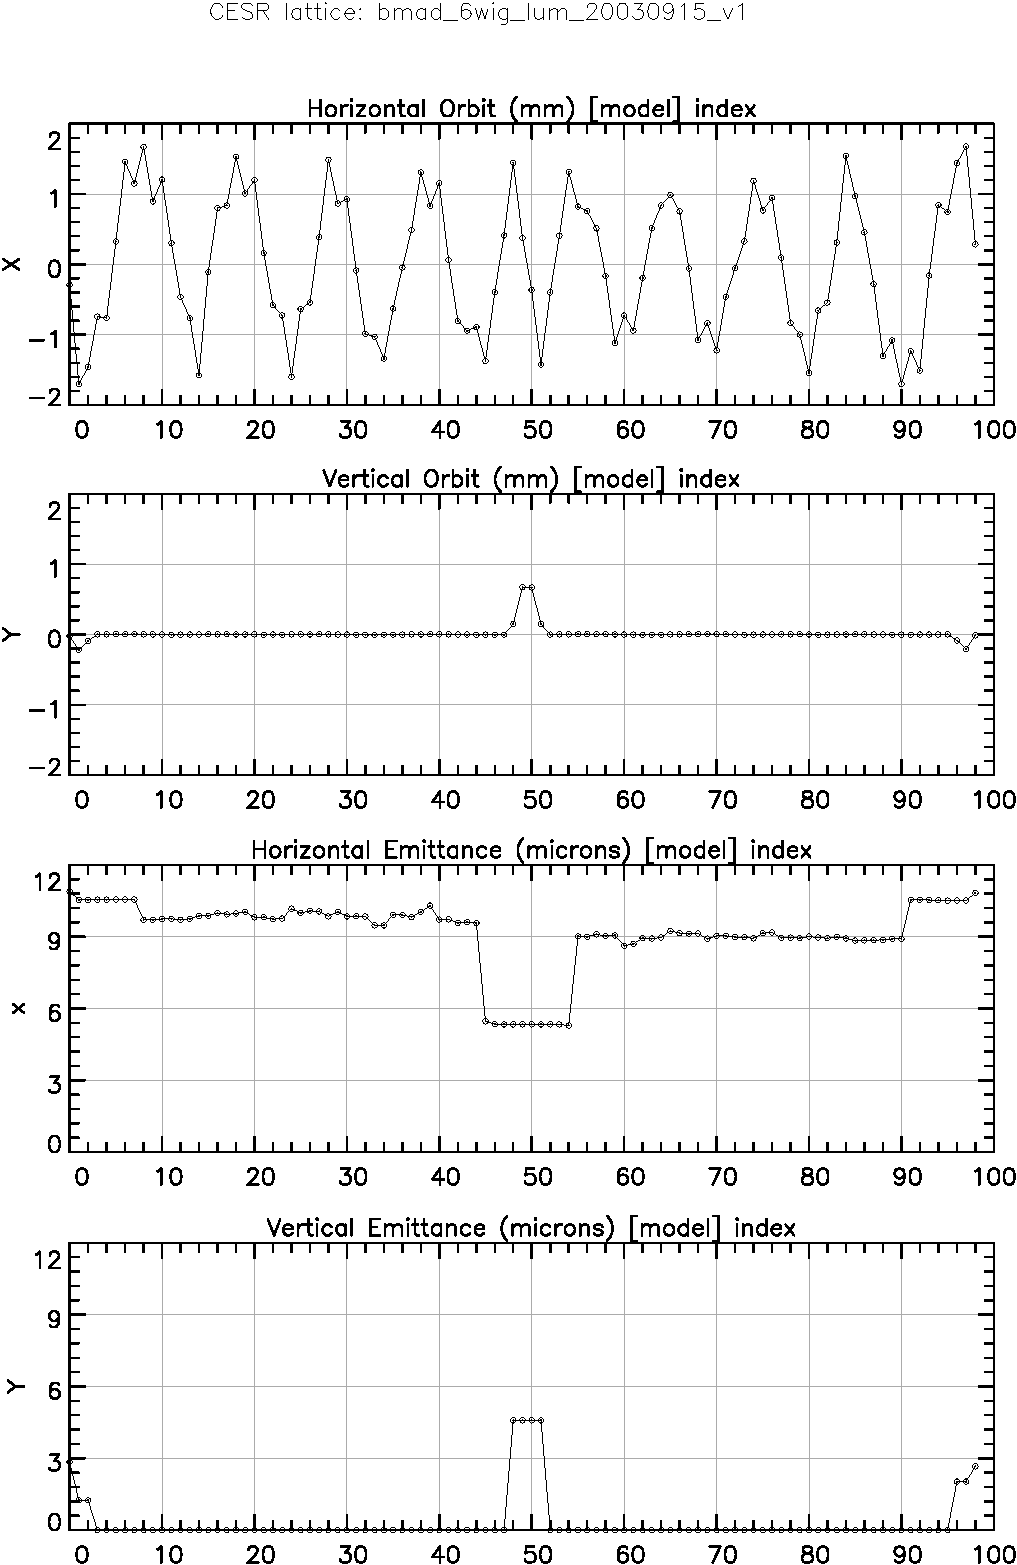
\includegraphics[width=5in]{plot-emittance.pdf}
  \caption{Custom data type: non-normalized emittance}
  \label{f:plot.emittance}
\end{figure}

%----------------------------------------------------------------
\section{Reading in Measured Data Example}
\label{s:cust.read.example}

This section shows how to construct a customized version of \tao, called \vn{ping_tao}, to read in
measured data for analysis. This example uses data from the Fermilab proton recirculation. The data
is obtained by measuring the orbit turn-by-turn of a beam that has been initially pinged to give it
a finite oscillation amplitude.

The files for constructing \vn{ping_tao} can be found
in the directory
\begin{example}
  bmad-doc/tao_examples/custom_tao_with_measured_data
\end{example}
The files in this directory are as follows:
\begin{description}
  \item[CMakeLists.txt, cmake.ping_tao] \Newline
Script files for creating \vn{ping_tao}. See Sec.~\sref{s:cust.init}.
  \item[README] \Newline
The \vn{README} file gives some instructions on how to create \vn{ping_tao}
  \item[RRNOVAMU2E11172016.bmad] \Newline
Lattice file for the proton recirculation ring.
  \item[data] \Newline
Directory where some ping data is stored
  \item[tao.init] \Newline
\tao initialization file defining the appropriate data and variable structures (\sref{s:init.begin})
  \item[tao.startup] \Newline
File with some command that are executed when \tao is started. These commands will read in
and plot some data.
  \item[tao_hook_command.f90] \Newline
Custom code for reading in ping data. The template used to construct this file is at
\vn{tao/hook/tao_hook_command.f90} (\sref{s:hook.command}).
  \item[tao_plot.init] \Newline
File for defining plot parameters (\sref{s:init.plot}).
  \item[tao_program.f90] \Newline
copy of the \vn{tao/program/tao_program.f90} file (\sref{s:cust.init}).
\end{description}

After creating the \vn{ping_tao} program (see the \vn{README} file), the program can be run by going
to the custom_tao_with_measured_data directory and using the command:
\begin{example}
	../production/bin/ping_tao
\end{example}

The customized \vn{tao_hook_command} routine implements a custom command called
\vn{pingread}.  This command will read in ping data. Ping data is the amplitude and phase
of the beam oscillations at a BPM for either the \vn{a-mode} or \vn{b-mode} oscillations.
See the write up on ping data types in Sec.~\sref{s:data.types} under \vn{ping_a.amp_x},
and \vn{ping_b.amp_x} for more details.

The data files in the \vn{data} directory contain data for either the \vn{a-mode} or \vn{b-mode}
ping at either the horizontal or vertical BPMs.

The syntax of the \vn{pingread} command is:
\begin{example}
  pingread <mode> <filename> <data_or_ref>
\end{example}
The first argument, \vn{<mode>}, should be either ``\vn{a_mode}'' ``\vn{b_mode}'' indicating wether
the data is for the \vn{a-mode} \vn{b-mode} analysis (a better setup would encode this information
in the data file itself). The second argument, \vn{filename} is the name of the data file, and the
third argument, \vn{data_or_ref} should be ``\vn{data}'' or ``\vn{reference}'' indicating that the
data is to be read into the \vn{meas_value} or \vn{ref_value} of the appropriate
\vn{tao_data_struct}.

%----------------------------------------------------------------
\subsection{Analysis of the tao_hook_command.f90 File}
\label{s:hook.cmd.anal}

The first part of the \vn{tao_hook_command} routine parses the command line to see if the
\vn{pingread} command is present. The relevant code, somewhat condensed, is:
\begin{example}
  subroutine tao_hook_command (command_line, found)

  !!!! put your list of hook commands in here. 

  character(16) :: cmd_names(1) = [character(16):: 'pingread']  

  ! "found" will be set to TRUE if the command is found.

  found = .false.

  ! strip the command line of comments

  call string_trim (command_line, cmd_line, ix_line)
  ix = index(cmd_line, '!')
  if (ix /= 0) cmd_line = cmd_line(:ix-1)        ! strip off comments

  ! blank line => nothing to do

  if (cmd_line(1:1) == '') return

  ! match first word to a command name
  ! If not found then found = .false.

  call match_word (cmd_line(:ix_line), cmd_names, ix_cmd, .true., .true., cmd_name)
  if (ix_cmd < 0) then
    call out_io (s_error$, r_name, 'AMBIGUOUS HOOK COMMAND')
    found = .true.
    return
  endif

  found = .true.
  call string_trim (cmd_line(ix_line+1:), cmd_line, ix_line)
\end{example}

Note: To quickly find information on routines and structures, use the \vn{getf} and \vn{listf}
scripts as explained in the \bmad manual. For example, typing ``\vn{getf string_trim}'' on the
system command line will give information on the string_trim subroutine.

The above code tests to see if the command is \vn{pingread} and, if not, returns without doing
anything.

If the \vn{pingread} command is found, the rest of the command line is parsed to get the
\vn{<mode>}, \vn{<filename>}, and \vn{<data_or_ref>} arguments.

In the \vn{tao.init} file, a \vn{tune} d2 datum is setup to have two \vn{d1} datum arrays One for
the \vn{a}-mode tune and one for the \vn{b}-mode tune:
\begin{example}
  \&tao_d2_data
    d2_data%name = "tune"
    universe = '*'  ! apply to all universes
    n_d1_data = 2
  /

  \&tao_d1_data
    ix_d1_data = 1
    d1_data%name = "a"
    default_weight = 1e6
    ix_min_data = 1
    ix_max_data = 1
  /

  \&tao_d1_data
    ix_d1_data = 2
    d1_data%name = "b"
    default_weight = 1e6
    ix_min_data = 1
    ix_max_data = 1
  /
\end{example}
And each \vn{d1} array has only one datum since the \vn{a}-mode and \vn{b}-mode tunes have only one
value associated with them (as opposed to, say an orbit which will have multiple values from
different BPMs).

In a data file there is a header section which, among other things, records the tune.
In a line beginning with the word ``\vn{Tune}''. Example:
\begin{example}
                   Horz         Vert         Sync.                           
   Tune           ( .452444)   ( .404434)   ( 0      ) 2p                    
\end{example}

In the \vn{tao_hook_command} file, after the arguments are parsed, the header part of the
data file is read to extract the tune datums:
\begin{example}
  type (tao_d2_data_array_struct), allocatable :: d2(:)
  ...
  if (line(1:4) == 'Tune') then
    call tao_find_data (err, 'tune', d2_array = d2)
    if (size(d2) /= 1) then
      call out_io (s_fatal$, r_name, 'NO TUNE D2 DATA STRUCTURE DEFINED!')
      return
    endif
\end{example}
The call to \vn{tao_find_data} looks for a \vn{d2} data structure named \vn{tune}. This structure is
setup in the \vn{tao.init} file. Alternatively, the \vn{ping_tao} program could be configured to
automatically setup the appropriate data and/or variable structures via the \vn{tao_hook_init1}
routine (\sref{s:hook.init}).

The returned value from the call to \vn{tao_find_data} is an array called \vn{d2} of type
\vn{tao_d2_data_array_struct}. \vn{d2} holds an array of pointers to all \vn{d2_data_struct}
structures it can find. In general, there could be multiple such structures if multiple universes
are being used or if the match string, in this case \vn{'tune'}, contained wild card characters. In
this case, the expectation is that there will only one universe used and thus there should be one
and only one structure that matches the name \vn{tune}. This structure will be pointed to by
\vn{d2(1)%d2}. The appropriate datums, will be:
\begin{example}
  d2(1)%d2%d1(1)%d(1)   ! a-mode tune
  d2(1)%d2%d1(1)%d(2)   ! b-mode tune
\end{example}
The values read from the data file are put in these datums via the code:
\begin{example}
  if (data_or_ref == 'data') then
    d2(1)%d2%d1(1)%d(1)%meas_value = twopi * (data_tune_a + nint(design_tune_a))
    d2(1)%d2%d1(1)%d(1)%good_meas = .true.
    d2(1)%d2%d1(2)%d(1)%meas_value = twopi * (data_tune_b + nint(design_tune_b))
    d2(1)%d2%d1(2)%d(1)%good_meas = .true.
  else
    d2(1)%d2%d1(1)%d(1)%ref_value = twopi * (data_tune_a + nint(design_tune_a))
    d2(1)%d2%d1(1)%d(1)%good_ref = .true.
    d2(1)%d2%d1(2)%d(1)%ref_value = twopi * (data_tune_b + nint(design_tune_b))
    d2(1)%d2%d1(2)%d(1)%good_ref = .true.
  endif      
\end{example}

The next step is to setup pointers to the appropriate data arrays to receive the ping data.
In the data file the ping data looks like:
\begin{example}
  BPM           Phase    Ampl.   RMSdev     Beta  bml_psi *Calib Old_Cal     
  R:HP222    -0.27314  0.46085    0.078    1.863  0.35183                         
  R:HP224    -0.05939  0.28277    0.143    0.701 -0.43442                         
  R:HP226     0.23140  0.31712    0.075    0.882 -0.14363                         
  ... etc ...
\end{example}
The ``\vn{H}'' in \vn{R:HP222}, etc. indicates that the data is from BPMs that only measure the
horizontal displacement of the beam. Alternatively, a ``\vn{V}'' would indicate data from vertical
measurement BPMs.

In the \vn{tao_hook_command} file the data pointers are setup by the code:
\begin{example}
  type (tao_d1_data_array_struct), allocatable, target :: d1_amp_arr(:), d1_phase_arr(:)
  ...
  if (line(3:3) == 'H') then
    if (mode == 'a_mode') then
      call tao_find_data (err, 'ping_a.amp_x', d1_array = d1_amp_arr)
      call tao_find_data (err, 'ping_a.phase_x', d1_array = d1_phase_arr)
    else 
      call tao_find_data (err, 'ping_b.amp_x', d1_array = d1_amp_arr)
      call tao_find_data (err, 'ping_b.phase_x', d1_array = d1_phase_arr)
    endif
  elseif (line(3:3) == 'V') then
    if (mode == 'a_mode') then
      call tao_find_data (err, 'ping_a.amp_y', d1_array = d1_amp_arr)
      call tao_find_data (err, 'ping_a.phase_y', d1_array = d1_phase_arr)
    else 
      call tao_find_data (err, 'ping_b.amp_y', d1_array = d1_amp_arr)
      call tao_find_data (err, 'ping_b.phase_y', d1_array = d1_phase_arr)
    endif
\end{example}
\vn{line(3:3)} is either \vn{H} or \vn{V} indicating horizontal or vertical orbit measuring BPMs. In
this case, the call to the \vn{tao_find_data} routine returns \vn{d1} data arrays to the amplitude
data (\vn{d1_amp_arr}) and phase data (\vn{d1_phase_arr}).  Just like the tune data, since it is
assumed only one universe is being used, there should be one and only \vn{d1} structure for the
phase and only one \vn{d1} structure for the amplitude:
\begin{example}
  d1_amp_arr(1)%d1      ! d1 struucture for the amplitude data
  d1_phase_arr(1)%d1    ! d1 struucture for the phase data
\end{example}
To save on typing, and make the code clearer, pointers are used to point to these structures:
\begin{example}
  type (tao_d1_data_struct), pointer :: d1_phase, d1_amp
  ...
  d1_amp => d1_amp_arr(1)%d1
  d1_phase => d1_phase_arr(1)%d1
\end{example}
The array of datums for the amplitude and phase data will be \vn{d1_amp%d(:)} and
\vn{d1_phase%d(:)} respectively.

After the \vn{d1_amp} and \vn{d1_phase} pointers have been set, there is a loop over all the lines
in the file to extract the ping data. One problem faced is that the order of the data in the file is
not the same as the order of the data in \vn{d1} structures.  [The data in the file is sorded in
increasing numberical order in the BPM name while the order in the \vn{d1} structures is sorted by
increasing logitudinal s-position.]  To get around this problem, the BPM name in the file is used to
locate the appropriate datum (the associated BPM element name is stored in the \vn{%ele_name}
component of the datums):
\begin{example}
  character(140) :: cmd_word(12), ele_name
  ... 
  call tao_cmd_split (line, 4, cmd_word, .false., err)
  read (cmd_word(2), *) r1
  read (cmd_word(3), *) r2
  ele_name = cmd_word(1)
  datum_amp => tao_pointer_to_datum(d1_amp, ele_name(3:))
  datum_phase => tao_pointer_to_datum(d1_phase, ele_name(3:))
\end{example}
The \vn{line} string holds a line from the data file, the call to \vn{tao_cmd_split} splits the line
into word chunks and puts them into the array \vn{cmd_word(:)}.  \vn{cmd_word(1)} holds the first
word which is the BPM name with ``\vn{R:}'' prepended to the name. The calls to
\vn{tao_pointer_to_datum} return pointers, \vn{datum_amp} and \vn{datum_phase}, to the approbriate
datums given the BPM name.

After the appropriate datums have been identified, the ping data values read from the data
file, \vn{r1} and \vn{r2}, are used to set the appropriate components:
\begin{example}
  if (data_or_ref == 'data') then
    datum_phase%good_meas = .true.
    datum_amp%meas_value = r2
    datum_amp%good_meas = .true.
  else
    datum_phase%good_ref = .true.
    datum_amp%ref_value = r2
    datum_amp%good_ref = .true.
  endif
\end{example}

One problem is that individual data phase data points can be off by factors of $2\pi$. To correct
this, the measured phase values are shifted by factors of $2\pi$ so that they are within $\pm\pi$ of
the design values. There is an added ``branch cut'' problem here in that, even without the factors
of $2\pi$ problem, the measured phases will be off from the design values by some arbitrary amount
(determined by how the zero phase is defined in the program that created the data file). If this
difference between the zero phase of the data and the zero phase of design lattice (in the design
lattice, the phase is taken to be zero at the beginning of the lattice) is close enough to $\pi$,
the shifting of the phases by factors of $2\pi$ will not be correct. For this reason, a best guess
as to what the offset is is used in the calculation to avoid the branch cut problem:
\begin{example}
  rms_best = 1e30

  do i = 1, 20
    offset = i / 20.0
    data = data + nint(design + offset - data)
    rms = sum((data - design - offset)**2, mask = ok)
    if (rms < rms_best) then
      offset_best = offset
      rms_best = rms
    endif
  enddo

  data = data + nint(design + offset_best - data)
\end{example}

\chapter{Tao Structures}
\index{structures in tao}
\label{c:structures}

This chapter gives an overview of the structures (classes) used in \tao.  Knowledge of the
structures is needed in order to create custom versions of \tao. See Chapter \sref{c:custom.tao} for
details of how to create custom \tao versions.

%-----------------------------------------------------------------
\section{Overview}
\index{programming!overview}

The \tao code files are stored in the following directories:
\begin{example}
  tao/code
  tao/hooks
  tao/program
\end{example}
Here \vn{tao} is the root directory of \tao. Ask your local guru
where to find this directory.

The files in \vn{tao/code} should not be modified when creating custom versions of \tao. The files
in \vn{tao/hooks}, as explained in Chapter \sref{c:custom.tao}, are templates used for
customization. Finally, the directory \vn{tao/program} holds the program file \vn{tao_program.f90}.

The structures used by tao are defined in the file \vn{tao_struct.f90}.  All \tao structures begin
with the prefix \vn{tao_} so any structure encountered that does not begin with \vn{tao_} must be
defined in some other library The \vn{getf} and \vn{listf} commands can be used to quickly get
information on any structure. See the \bmad manual for more details.

%-----------------------------------------------------------------
\section{tao_super_universe_struct}
\label{s:super.uni.struct}
\index{tao_super_universe_struct}

The "root" structure in \tao is the \vn{tao_super_universe_struct}. 
The definition of this structure is:
\begin{example}
  type tao_super_universe_struct
    type (tao_global_struct) global                      ! Global variables.
    type (tao_common_struct) :: com                      ! Global variables
    type (tao_plotting_struct) :: plotting               ! Plot parameters.
    type (tao_v1_var_struct), allocatable :: v1_var(:)   ! V1 Variable array
    type (tao_var_struct), allocatable :: var(:)         ! Array of all variables.
    type (tao_universe_struct), allocatable :: u(:)      ! Array of universes.
    type (tao_mpi_struct) mpi
    integer, allocatable :: key(:)
    type (tao_building_wall_struct) :: building_wall
    type (tao_wave_struct) :: wave 
    integer n_var_used
    integer n_v1_var_used
    type (tao_cmd_history_struct) :: history(1000)        ! command history
  end type
\end{example}
An instance of this structure called \vn{s} is defined in \vn{tao_struct.f90}:
\begin{example}
  type (tao_super_universe_struct), save, target :: s
\end{example}
This \vn{s} variable is common to all of \tao's routines and serves as a giant common block for \tao.

The components of the \vn{tao_super_universe_struct} are:
  \begin{description}
  \index{tao_global_struct}
  \item[\%global] \Newline
The \vn{%global} component contains global variables that a user can set
in an initialization file.
See \sref{s:globals} for more details.
  \index{tao_common_struct}
  \item[\%com] \Newline
The \vn{%com} component is for global variables that are not directly
user accessible.
  \index{tao_plotting_struct}
  \item[\%plot_page] \Newline
The \vn{%plot_page} component holds parameters used in plotting (\sref{s:s.plot.page}).
  \index{tao_v1_var_struct}
  \item[\%v1_var(:)] \Newline
The \vn{%v1_var(:)} component is an array of all the \vn{v1_var} blocks
(\sref{c:var}) that the user has defined (\sref{s:s.v1.var}).
  \index{tao_var_struct}
  \item[\%var(:)]
The \vn{%var(:)} array holds a list of all variables (\sref{c:var})
that the user has defined (\sref{s:s.var}).
  \index{tao_universe_struct}
  \item[\%u(:)] \Newline
The \vn{%u(:)} component is an array of universes (\sref{s:universe}) (\sref{s:s.u}).
  \index{tao_mpi_struct}
  \item[\%mpi] \Newline
The \vn{%mpi} component holds parameters needed for parallel processing (\sref{s:s.mpi}).
  \item[\%key(:)] \Newline
The \vn{%key(:)} component is an array of indexes used for key bindings 
(\sref{s:key.bind}). 
  \index{tao_building_wall_struct}
  \item[\%building_wall] \Newline
The \vn{%building_wall} component holds parameters associated
with a building wall (\sref{s:building.wall}).
  \index{tao_wave_struct}
  \item[\%wave] \Newline
The \vn{%wave} component holds parameters needed for the wave analysis
(\sref{c:wave}).
  \item[\%history] \Newline
The \vn{%history} component holds the command history (\sref{s:s.history}).
  \end{description}

%-----------------------------------------------------------------
\section{s\%plot_page Component}
\label{s:s.plot.page}

The \vn{s%plot_page} component of the \vn{super universe} (\sref{s:super.uni.struct}) holds plotting
information and is initialized in the routine \vn{tao_init_plotting}. \vn{s%plot_page} is a
\vn{tao_plot_page_struct} structure which has components:
\begin{example}
  type tao_plot_page_struct
    type (tao_title_struct) title             ! Title at top of page.
    type (tao_title_struct) subtitle          ! Subtitle at top of page.
    type (qp_rect_struct) border              ! Border around plots edge of page.
    type (tao_drawing_struct) :: floor_plan
    type (tao_drawing_struct) :: lat_layout
    type (tao_shape_pattern_struct), allocatable :: pattern(:)
    type (tao_plot_struct), allocatable :: template(:)  ! Templates for the plots.
    type (tao_plot_region_struct), allocatable :: region(:)
    character(8) :: plot_display_type = 'X'   ! 'X' (X11) or 'TK'
    real(rp) size(2)                          ! width and height of window in pixels.
    real(rp) :: text_height = 12              ! In points. Scales the height of all text
    real(rp) :: main_title_text_scale  = 1.3  ! Relative to text_height
    real(rp) :: graph_title_text_scale = 1.1  ! Relative to text_height
    real(rp) :: axis_number_text_scale = 0.9  ! Relative to text_height
    real(rp) :: axis_label_text_scale  = 1.0  ! Relative to text_height
    real(rp) :: legend_text_scale      = 0.7  ! Relative to text_height
    real(rp) :: key_table_text_scale   = 0.9  ! Relative to text_height
    real(rp) :: curve_legend_line_len  = 50   ! Points
    real(rp) :: curve_legend_text_offset = 10 ! Points
    real(rp) :: floor_plan_shape_scale = 1.0
    real(rp) :: lat_layout_shape_scale = 1.0
    integer :: n_curve_pts = 401              ! Default number of points for plotting a smooth curve.
    integer :: id_window = -1                 ! X window id number.
    logical :: delete_overlapping_plots = .true. ! Delete overlapping plots when a plot is placed?
  end type
\end{example}

\begin{description}
  \item[\%template(:)] \Newline
The \vn{%template(:)} array contains the array of plot templates defined by the user (\sref{s:template}) and/or
the default plot templates which are created in the routine \vn{tao_init_plotting}.
  \item[\%region(:)] \Newline
The \vn{%region(:)} array contains the plot regions. Each element in the array is a \vn{tao_plot_region_struct}
structure:
\begin{example}
  type tao_plot_region_struct
    character(40) :: name = ''     ! Region name. Eg: 'r13', etc.
    type (tao_plot_struct) plot    ! Plot associated with this region
    real(rp) location(4)           ! [x1, x2, y1, y2] location on page.
    logical :: visible = .false.   ! To draw or not to draw.
    logical :: list_with_show_plot_command = .true.  ! False used for default plots to 
                                                     !  shorten the output of "show plot"
  end type
\end{example}
Then \vn{place} command finds the appropriate plot in the \vn{s%plot_page%template(:)} array and
copies it to the \vn{s%plot_page%region(i)%plot} component where \vn{i} is the index of the region
specified by the \vn{place} command.
\end{description}

%-----------------------------------------------------------------
\section {s\%v1_var Component}
\label{s:s.v1.var}

The \vn{s%v1_var(:)} array holds the list of \vn{v1} variable blocks (\sref{c:var}).
This array is initialized in the routine \vn{tao_init_variables}.
The range of valid elements in this array goes from 1 to \vn{s%n_v1_var_used}.
Each element of this array is a \vn{tao_v1_var_struct} structure:
\begin{example}
  type tao_v1_var_struct
    character(40) :: name = ''       ! V1 variable name. Eg: 'quad_k1'.
    integer ix_v1_var                ! Index to s%v1_var(:) array
    type (tao_var_struct), pointer :: v(:) => null()
                                     ! Pointer to the appropriate section in s%var.
  end type
\end{example}

The \vn{%ix_v1_var} component is the index of the element in the \vn{s%v1_var(:)} array.
That is, \vn{s%v1_var(1)%ix_v1_var} = 1, etc. This is useful when debugging. 

The \vn{%v(:)} component is a pointer to the appropreiate block in the \vn{s%var(:)} array
(\sref{s:s.var}) which contain the individual variables associated with the particular
\vn{v1} variable block. 

%-----------------------------------------------------------------
\section {s\%var Component}
\label{s:s.var}

The \vn{s%var(:)} array holds the list complete list of all variables (\sref{c:var}).  This array is
initialized in the routine \vn{tao_init_variables}. The range of valid variables goes from 1 to
\vn{s%n_var_used}. Each element in the \vn{s%v1_var(:)} array (\sref{s:s.v1.var}) has a pointer to
the section of the \vn{s%var(:)} array holding the variables associated with \vn{v1} block. Using a
single array of variables simplifies code where one wants to simply loop over all variables (for
example, during optimization).

Each element of the \vn{s%var(:)} array is a \vn{tao_var_struct} structure:
\begin{example}
  type tao_var_struct
    character(40) :: ele_name = ''    ! Associated lattice element name.
    character(40) :: attrib_name = '' ! Name of the attribute to vary.
    character(40) :: id = ''          ! Used by Tao extension code. Not used by Tao directly.
    type (tao_var_slave_struct), allocatable :: slave(:)
    type (tao_var_slave_struct) :: common_slave
    integer :: ix_v1 = 0              ! Index of this var in the s%v1_var(i)%v(:) array.
    integer :: ix_var = 0             ! Index number of this var in the s%var(:) array.
    integer :: ix_dvar = -1           ! Column in the dData_dVar derivative matrix.
    integer :: ix_attrib = 0          ! Index in ele%value(:) array if appropriate.
    integer :: ix_key_table = 0       ! Has a key binding?
    real(rp), pointer :: model_value => null()     ! Model value.
    real(rp), pointer :: base_value => null()      ! Base value.
    real(rp) :: design_value = 0      ! Design value from the design lattice.
    real(rp) :: scratch_value = 0     ! Scratch space to be used within a routine.
    real(rp) :: old_value = 0         ! Scratch space to be used within a routine.
    real(rp) :: meas_value = 0        ! The value when the data measurement was taken.
    real(rp) :: ref_value = 0         ! Value when the reference measurement was taken.
    real(rp) :: correction_value = 0  ! Value determined by a fit to correct the lattice.
    real(rp) :: high_lim = -1d30      ! High limit for the model_value.
    real(rp) :: low_lim = 1d30        ! Low limit for the model_value.
    real(rp) :: step = 0              ! Sets what is a small step for varying this var.
    real(rp) :: weight = 0            ! Weight for the merit function term.
    real(rp) :: delta_merit = 0       ! Diff used to calculate the merit function term.
    real(rp) :: merit = 0             ! merit_term = weight * delta^2.
    real(rp) :: dMerit_dVar = 0       ! Merit derivative.
    real(rp) :: key_val0 = 0          ! Key base value
    real(rp) :: key_delta = 0         ! Change in value when a key is pressed.
    real(rp) :: s = 0                 ! longitudinal position of ele.
    character(40) :: merit_type = ''  ! 'target' or 'limit'
    logical :: exists = .false.       ! See above
    logical :: good_var = .false.     ! See above
    logical :: good_user = .true.     ! See above
    logical :: good_opt = .false.     ! See above
    logical :: good_plot = .false.    ! See above
    logical :: useit_opt = .false.    ! See above
    logical :: useit_plot = .false.   ! See above
    logical :: key_bound = .false.    ! Variable bound to keyboard key?
    type (tao_v1_var_struct), pointer :: v1 => null() ! Pointer to the parent.
  end type tao_var_struct
\end{example}

  \begin{description}
  \item[\%exists] \Newline
The variable exists. Non-existent variables can serve as place holders in the \vn{s%var array}.
  \item[\%good_var] \Newline
The variable can be varied. Used by the lm optimizer to veto variables that do not change the merit
function.
  \item[\%good_user] \Newline
What the user has selected using the use, veto, and restore commands.
  \item[\%good_opt] \Newline
Not modified by Tao. Setting is reserved to be done by extension code.
  \item[\%good_plot] \Newline
Not modified by Tao. Setting is reserved to be done by extension code.
  \item[\%useit_opt] \Newline
Variable is to be used for optimizing:
\begin{example}
  %useit_opt = %exists & %good_user & %good_opt & %good_var
\end{example}
  \item[\%useit_plot] \Newline
If True variable is used in plotting variable values:
\begin{example}
  %useit_plot = %exists & %good_plot & %good_user
\end{example}
\end{description}

%-----------------------------------------------------------------
\section {s\%u Component}
\label{s:s.u}

The \vn{s%u(:)} array holds the \tao universes (\sref{s:universe}). Each element
of this array is a \vn{tao_universe_struct} structure:
\begin{example}
  type tao_universe_struct
    type (tao_universe_struct), pointer :: common => null()
    type (tao_lattice_struct), pointer :: model, design, base
    type (tao_beam_struct) beam
    type (tao_dynamic_aperture_struct) :: dynamic_aperture
    type (tao_universe_branch_struct), pointer :: uni_branch(:) ! Per element information
    type (tao_d2_data_struct), allocatable :: d2_data(:)   ! The data types
    type (tao_data_struct), allocatable :: data(:)         ! Array of all data.
    type (tao_ping_scale_struct) ping_scale
    type (lat_struct) scratch_lat                          ! Scratch area.
    type (tao_universe_calc_struct) calc                   ! What needs to be calculated?
    real(rp), allocatable :: dModel_dVar(:,:)              ! Derivative matrix.
    integer ix_uni                         ! Universe index.
    integer n_d2_data_used                 ! Number of used %d2_data(:) components.
    integer n_data_used                    ! Number of used %data(:) components.
    logical is_on                          ! universe turned on
    logical picked_uni                     ! Scratch logical.
  end type
\end{example}

%-----------------------------------------------------------------
\section {s\%mpi Component}
\label{s:s.mpi}

The \vn{s%mpi} component holds information that is used when running \tao multi-threaded.


%-----------------------------------------------------------------
\section {s\%key Component}
\label{s:s.key}

The value of \vn{%key(i)} is the index in the \vn{%var(:)} array associated with the $i$\th key.

%-----------------------------------------------------------------
\section {s\%building_wall Component}
\label{s:s.building.wall}

%-----------------------------------------------------------------
\section {s\%wave Component}
\label{s:s.wave}

%-----------------------------------------------------------------
\section {s\%history Component}
\label{s:s.history}


%----------------------------------------------------------------
\part{Bibliography}

\cleardoublepage
\phantomsection
\addcontentsline{toc}{chapter}{Bibliography}
\begin{thebibliography}{99}

\bibitem[Bma06]{b:bmad}
D. Sagan,
"Bmad: A Relativistic Charged Particle Simulation Library"
Nuc.\ Instrum.\ \& Methods Phys.\ Res.\ A, {\bf 558}, pp 356-59 (2006).

The Bmad Manual can be optained at:
\hfill\break
\hspace*{20pt} 
\url{www.classe.cornell.edu/bmad}

\bibitem[Bengt97]{b:bengtsson}
J.~Bengtsson,
``The Sextupole Scheme for the Swiss Light Source (SLS): An Analytic Approach,''
SLS Note 9/97, Paul Scherrer Institut, (1997).

\bibitem[Blender]{b:blender}
\vn{Blender} web page:
\hfill\break
\hspace*{20pt} 
\url{blender.org/}

\bibitem[Fra11]{b:emit}
A.~Franchi, L.~Farvacque, J.~Chavanne, F.~Ewald, B.~Nash, K.~Scheidt, and R.~Tom\',
``Vertical emittance reduction and preservation in electron storage rings via resonance driving terms correction'',
Phys. Rev. ST Accel. Beams,
{\bf 14}, 3, 034002, (2011). 
\hfill\break
\hspace*{20pt}
\url{link.aps.org/doi/10.1103/PhysRevSTAB.14.034002}

\bibitem[CBETA19]{b:cbeta}
C.~Gulliford, A.~Bartnik, J.~Scott~Berg, J.~Dobbins, A.~Nunez-delPrado, and D.~Sagan,
``Experience With CBETA Online Modeling Tools'',
13th International Computational Accelerator Physics Conference, 2019.

\bibitem[NR92]{b:nr}
W.~Press, B.~Flannery, S.~Teukolsky, W.~Wetterling,
{\em Numerical Recipes in Fortran, the Art of Scientific Computing},
Second Edition, Cambridge University Press, New York (1992)

\bibitem[Montague]{b:w}
B. W. S. L. Montague, “Linear Optics For Improved Chromaticity Correction,” 
CERN, Geneva, Tech. Rep. CERN-LEP-Note-165. LEP-Note-165, 1979. 
\url{http://cds.cern.ch/record/443342}

\bibitem[Saf97]{b:orm}
J. Safranek, ``Experimental determination of storage ring optics
using orbit response measurements'', NIM-A388, p. 27 (1997).

\bibitem[Sag99]{b:linear.coupled}
D. Sagan, and D. Rubin,
``Linear Analysis of Coupled Lattices,''
Phys. Rev. ST Accel. Beams 2, 074001 (1999).
\hfill\break
\hspace*{20pt}
\url{https://journals.aps.org/prab/abstract/10.1103/PhysRevSTAB.2.074001}

\bibitem[Sag00a]{b:beta.meas}
D. Sagan, R. Meller, R. Littauer, and D. Rubin,
``Betatron phase and coupling measurement at the Cornell Electron/Positron Storage Ring'', 
Phys. Rev. ST Accel. Beams 3, 092801 (2000).
\hfill\break
\hspace*{20pt}
\url{link.aps.org/doi/10.1103/PhysRevSTAB.3.092801}

\bibitem[Sag00b]{b:wave}
D. Sagan,
``Betatron phase and coupling correction at the Cornell Electron/Positron
Storage Ring'', Phys. Rev. ST Accel. Beams 3, 102801 (2000).
\hfill\break
\hspace*{20pt}
\url{link.aps.org/doi/10.1103/PhysRevSTAB.3.102801}

\bibitem[Sto96]{b:de}
R.~Storn, and K.~V.~Price, "Minimizing the real function of the
ICEC'96 contest by differential evolution" IEEE conf. on Evolutionary
Computation, 842-844 (1996).

\bibitem[Wang12]{b:wang}
C.~Wang,
``Explicit formulas for 2nd-order driving terms due to sextupoles and
chromatic effects of quadrupoles,''
ANL/APS/LS-330, Argonne National Laboratory, (2012).

\bibitem[Wil00]{b:wille}
Klaus Wille, {\em The Physics of Particle Accelerators: An Introduction},
Translated by Jason McFall, Oxford University Press (2000).

\end{thebibliography}


\printindex

\end{document}
